\documentclass[11pt,letterpaper]{report}
\usepackage[margin=1in]{geometry}
\usepackage[latin1]{inputenc}
\usepackage{url}
\usepackage{hyperref}
\usepackage{doi}
\usepackage{breakurl}
\urlstyle{same} 			% Use same font type and size for url as the text.

\usepackage{natbib}
\usepackage{fancyhdr}
\pagestyle{fancy}
\usepackage[hang]{footmisc}
\usepackage[textfont={bf}]{caption}
\usepackage{amsmath}
\usepackage{amsfonts}
\usepackage{amssymb}
\usepackage{graphicx}
\usepackage[version=3]{mhchem}
\usepackage[table,dvipsnames,svgnames,x11names]{xcolor}
\usepackage{color}
\usepackage{dcolumn}
\usepackage{booktabs}
\usepackage{pdflscape}
\usepackage{textcomp}
\usepackage{float}
\usepackage{subfig}
\usepackage{chngcntr}
\usepackage{needspace}
\counterwithout{figure}{chapter}
%\usepackage[usenames,dvipsnames,svgnames]{xcolor}
\definecolor{darkerGreen}{rgb}{0.702,0.800,0.510}
\definecolor{darkGreen}{rgb}{0.839,0.890,0.737}
\definecolor{liteGreen}{rgb}{0.918,0.945,0.867}
\definecolor{lightgray}{gray}{0.9}
\definecolor{lightblue}{rgb}{0.93,0.95,1.0}
\definecolor{URLBlue}{rgb}{0,0,0.5} % Define new color for hyperlinks
\hypersetup{
	colorlinks   = true,
	citecolor    = URLBlue,
	linkcolor    = URLBlue,
	urlcolor     = URLBlue
}

\definecolor{TableBorder}{rgb}{0.325,0.557,0.835}
%\definecolor{TableEven}{rgb}{0.8000,0.9216,0.9490}
\definecolor{TableEven}{rgb}{0.773,0.851,0.945}
\definecolor{TableOdd}{rgb}{1,1,1}

%\usepackage{pstricks,pst-node,pst-tree}

\usepackage{pgfplots}
\usetikzlibrary{matrix}
\usepgfplotslibrary{groupplots}

\pgfplotsset{compat=newest}
\pgfplotsset{every axis/.append style={line width=0.75pt},
   axis x line*=bottom, axis y line*=left}
\pgfsetplotmarksize{0pt}

\usetikzlibrary{shapes,arrows}
% Define block styles
\tikzstyle{decision} = [diamond, draw, fill=blue!20,
   text width=5.0em, text badly centered, node distance=3cm, inner sep=0pt]
\tikzstyle{block} = [rectangle, draw, fill=blue!20,
   minimum width=5cm, minimum height=2.0cm, text centered, text width=5cm,
   rounded corners, minimum height=4em]
\tikzstyle{smallblock} = [rectangle, draw, fill=blue!20,
   minimum width=2.5cm, minimum height=2.0cm, text centered, text width=2.5cm,
   rounded corners, minimum height=4em]
\tikzstyle{line} = [draw, -latex']
\tikzstyle{cloud} = [draw, ellipse,fill=red!20, node distance=5cm, minimum height=1.5cm]
\usepackage{tikzpagenodes}
\usetikzlibrary{calc}
\definecolor{GTAPBlue}{RGB}{27,66,115}
\definecolor{GTAPOrange}{RGB}{243,143,34}

\usepackage{forest}
\usetikzlibrary{shadows}
% RGB scale relative to 255
\definecolor{TableBorder}{rgb}{0.325,0.557,0.835}
%\definecolor{TableEven}{rgb}{0.8000,0.9216,0.9490}
\definecolor{TableEven}{rgb}{0.773,0.851,0.945}
\definecolor{TableOdd}{rgb}{1,1,1}
\newcommand\VRule[1][\arrayrulewidth]{\vrule width #1}
\definecolor{dkBlue}{rgb}{0.6157 0.7647 0.9020}
\definecolor{mdBlue}{rgb}{0.7412 0.8431 0.9333}
\definecolor{ltBlue}{rgb}{0.8706 0.9216 0.9686}

\usepackage{listings}
\input{../../../Word/Latex/gams}
\usepackage{extdash}
\newif\ifCESDetail
\CESDetailfalse

\begin{document}

\newcommand{\COT}{\ce{CO2}}
\newcommand{\localtextbulletone}
   {\textcolor{gray}{\raisebox{.45ex}{\rule{.7ex}{.7ex}}}}
\renewcommand{\labelitemi}{\localtextbulletone}
\newcommand{\overbar}[1]
   {\mkern 1.0mu\overline{\mkern-1.0mu#1\mkern-1.0mu}\mkern 1.0mu}
\lhead{}

% ---------- FIRST PAGE cover page with GTAP colors and logo

\pagestyle{empty}
\begin{tikzpicture}[overlay,remember picture]

    % Fill top rectangle with shaded orange

    \fill[GTAPOrange!20]
       ([yshift=2.0cm]current page.north west) rectangle ([yshift=-8.5cm]current page.north east);

    %  Make blue bar on extreme left
    %  Make orange bar to the right of the blue bar

    \fill[GTAPBlue]
      ([yshift=2.0cm]current page.north west) rectangle ([xshift=0.4cm]current page.south west);

    \fill[GTAPOrange,left color=GTAPOrange, right color=GTAPOrange!50]
       ([xshift=0.5cm,yshift=2.0cm]current page.north west) rectangle ([xshift=1.0cm]current page.south west);

    %  Insert main title and WP number

    \draw[GTAPOrange,thick] (13cm,-3cm)
       node[GTAPBlue,above left] {\Huge \textbf{\textsf{GTAP Technical Paper}}} --+ (0,3)
       % >>>> INSERT TP NUMBER HERE <<<<
       node[GTAPBlue,below right] {\LARGE \textbf{\textsf{TP/25/xx}}};

    %  Insert WP title and author(s)

    \node[yshift=-9cm,GTAPBlue] at (8.5cm,0cm) {\scalebox{1.5}
       {\textbf{The \underline{Env}ironmental \underline{I}mpact and
          \underline{S}ustainability \underline{A}pplied } } } ;
    \node[yshift=-10cm,GTAPBlue] at (8.5cm,0cm) {\scalebox{1.5}
       {\textbf{\underline{G}eneral
          \underline{E}quilibrium ({ENVISAGE}) Model, Version 11.0} } } ;
    \node[yshift=-12cm,GTAPBlue] at (8.5cm,0cm) {\scalebox{1}
       {\textbf{by Dominique van der Mensbrugghe}}};

    %  Insert Center's name and logo

    %  Insert Center's name and logo

    \node[yshift=-18cm,GTAPBlue] at (8.5cm,0cm)
       {\scalebox{0.45}{\includegraphics{GTAP_logo_CGTA_words.eps}}};

\end{tikzpicture}

\normalsize
\clearpage

% ---------- SECOND PAGE with copyright, edition(s), reference, etc.

\pagestyle{empty}

\vspace*{2cm}
\footnotesize
\noindent \textcopyright \, 2025 Center for Global Trade Analysis, Purdue University \\
All rights reserved.

\vspace{3cm}
%\noindent First edition: van der Mensbrugghe, Dominique, 2019. \\
%\hspace*{0.5cm} The Standard GTAP Model in Gams, Version 7 \\
%\hspace*{0.5cm} \emph{Journal of Global Economic Analysis}, 3(1): 1--83. \\
\noindent First edition: June 2019 \\
\noindent Second edition: March 2020 \\
\noindent Third edition: November 2021 \\
\noindent Third edition: April 2025 \\

\vspace{4cm}
\noindent \emph{Please cite using the following reference:} \\
\hspace*{0.25cm} van der Mensbrugghe, Dominique, 2025. \\
\hspace*{0.5cm} The Environmental Impact and Sustainability Applied \\
\hspace*{0.5cm} General Equilibrium (ENVISAGE) Model, Version 11.0 \\
\hspace*{0.5cm} GTAP Technical Paper, TP/25/xx \\
\hspace*{0.5cm} Center for Global Trade Analysis, Purdue University \\
\hspace*{0.5cm} West Lafayette, IN \\
\hspace*{0.5cm} \url{https://www...} \\

\vspace{2cm}
\noindent Center for Global Trade Analysis \\
Department of Agricultural Economics \\
Purdue University \\
West Lafayette, IN 47907 \\
\url{https://www.gtap.agecon.purdue.edu} \\
\clearpage

% ---------- THIRD PAGE internal cover page with title, author(s), abstract, etc.
\pagestyle{empty}

\vspace*{1cm}

\begin{center}

\Large \textbf{{The \underline{Env}ironmental \underline{I}mpact and
   \underline{S}ustainability \underline{A}pplied \underline{G}eneral
   \underline{E}quilibrium ({ENVISAGE}) Model, Version 11.0}} \\[2cm]

\large{Dominique van der Mensbrugghe\footnote{The Center for Global Trade Analysis,
   Purdue University, 403 Mitch Daniels Boulevard, West Lafayette, IN 47906.
   Corresponding e-mail: vandermd@purdue.edu.}
} \\ [1cm]

\today \\ [2cm]

\normalsize
\begin{minipage}{0.85\linewidth}
\textbf{Abstract: }
{This document's main purpose is to provide a full description
of the \textsc{Envisage} Model. \textsc{Envisage} is a global recursive dynamic
computable general equilibrium model developed originally at the {World Bank}.
\textsc{Envisage} has been developed to
assess the interactions between economies and the global environment as affected
by human-based emissions of greenhouse gases. At its core, \textsc{Envisage} is
a relatively standard recursive dynamic multi-sector multi-region CGE model. It
is complemented with an emissions and climate module that links
directly economic activities to changes in global mean temperature. And it
incorporates a feedback loop that links changes in temperature to impacts on
economic variables such as agricultural yields or damages created by sea level
rise [tbd]. One of the overall objectives of the development of
\textsc{Envisage} has been to provide a greater focus on the economics of
climate change for a more detailed set of developing countries as well as
greater attention to the potential economic damages. The model remains a work in
progress as there are several key features of the economics of climate change
that are planned to be incorporated.}
\end{minipage}
\end{center}

\vspace{2cm}
\begin{tabbing}
\hspace*{0.5cm} \textbf{JEL Codes:} \= {>>>> INSERT JEL CODES HERE <<<<} \\
\hspace*{0.5cm} \textbf{Keywords:}  \> {>>>> INSERT KEYWORDS HERE <<<<}\\
\end{tabbing}
\newpage

% ----------- NEXT PAGES include table of contents, list of table, list of figures

% Start page numbering with '2', title page should fit on one page, set
% page numbering to roman
\pagestyle{plain}
\pagenumbering{roman}
\setcounter{page}{2}

\tableofcontents
\newpage

\listoftables
\newpage

\listoffigures
\newpage

\setcounter{page}{1}
\pagenumbering{arabic}
\pagestyle{plain}
\renewcommand*{\thefootnote}{\arabic{footnote}}
\setcounter{footnote}{0}

\chapter{Introduction}
\renewcommand{\thepage}{\arabic{page}}% Arabic numerals for page counter
\setcounter{page}{1}

The purpose of this document is to provide a complete specification of the
equations of the \textsc{\underline{Env}ironmental} \textsc{\underline{I}mpact}
\textsc{and} \textsc{\underline{S}ustainability} \textsc{\underline{A}pplied}
\textsc{\underline{G}eneral} \textsc{\underline{E}quilibrium}
(\textsc{\textsc{ENVISAGE}}) \textsc{Model}. The \textsc{Envisage} Model is
designed to analyze a variety of issues related to the economics of climate
change:

\begin{itemize}
   \item Baseline emissions of \COT{} and other greenhouse gases
   \item Impacts of climate change on the economy
   \item Adaptation by economic agents to climate change
   \item Greenhouse gas mitigation policies---taxes, caps and trade
   \item The role of land use in future emissions and mitigation
   \item The distributional consequences of climate change impacts, adaptation
         and mitigation---at both the national and household level.
   \item Assessing projections of nutritional indicators and policies
   that impact nutrition pathways.
\end{itemize}

\textsc{Envisage} is intended to be flexible in terms of its dimensions. The
core database---that includes energy volumes and \COT{} emissions---is the GTAP
database, currently version 11B with a 2017 base year (see
\cite{AguiaretalJGEA2023}). The latter divides the world into 160
regions, of which 141 are individual countries and the other are region-based
aggregations.\footnote{The countries defined in GTAP cover well over 90 percent
of global GDP and population.} The database divides global production into 65
sectors---with extensive details for agriculture and food and energy (coal
mining, crude oil production, natural gas production, refined oil, electricity,
and distributed natural gas). Appendix~\ref{chap:GTAPDim} provides more detail.
Due to numerical and algorithmic constraints, a typical model is limited to some
20-30 sectors and 20-30 regions.

This document describes the current version of \textsc{Envisage}, which is still
in a developmental stage. This current version includes the following:

\begin{itemize}
   \item Capital vintage production technology that permits analysis of the
         flexibility of economies.
   \item {Two-level decomposition of domestic absorption into demand for domestic
         production and bilateral imports. This ranges from a simple version
         with a national agent optimizing each stage, to a full MRIO version
         with bilateral sourcing at the agent level. [Added 31-Oct-2020] The
         three specifications can co-exist, i.e. the model allows for any
         one of the three specifications to operate simultaneously and the choice can
         be both region- and sector-specific.}
   \item A detailed specification of energy demand in each economy.
   \item {[Added 31-OCT-2020]. The energy bundles---both in production and final demand---have been adjusted to allow for the traditional specification using a standard nested CES structure as well as the so-called additive version of the CES. The latter, which represents a different formulation of the logit specification, implies both volume and value additivity. It is more fully described in Appendix~\ref{chap:CESAppendix} and in \cite{DvdMPetersGTWP2020}. The Armington trade structure and
   the CET allocation of domestic supply have also been adapted to allow for the additive version of the CES and CET, respectively.}
   \item A resource depletion module for coal, oil and natural gas.
   \item The ability to introduce future alternative energy (or backstop)
         technologies [tbd]
   \item \COT{} emissions that are fuel and demand specific.
   \item Incorporation of the main Kyoto greenhouse gases (methane, nitrous
         oxide and the fluoridated gases) as well as a set of additional
         emissions (such as particulates, black carbon, etc.).
   \item A flexible system for incorporating any combination of carbon taxes,
         emission caps and tradable permits.
   \item {[Added 31-Oct-2020] A simplified climate module that links greenhouse gas emissions to
         atmospheric concentrations combined with a carbon cycle that leads to
         radiative forcing and temperature changes.}
   \item A water module that incorporates water use for irrigation by crop, and
         aggregate water demand in other parts of the economy.
   \item {[Added 21-Apr-2018] Government to government transfers have been
   incorporated. As more small developing countries are being included in the
   GTAP database and models, a more detailed accounting of the balance of
   payments is important to reflect macro balances.}
   \item {[Added 01-Dec-2018] The trade module now includes the \emph{ad valorem} equivalent (AVE) of non-tariff measures (NTMs). Unlike tariff revenues, the revenues generated by the NTMs can be allocated to private households and government---either domestic or foreign.}
   \item {[Added 01-Dec-2018] The make module has a new technology parameter that can be used to capture changes in post-harvest (or production) losses.}
   \item {[Added 01-Dec-2018] Household demand includes a new waste module, with the possibility of taxing
   household waste.}
   \item {[Added 20-Jan-2019] A research and development (R\&D) module has been added. R\&D expenditures add to the knowledge stock, however with a distributed lag structure. The knowledge stock influences an endogenous component of labor productivity growth.}
   \item {[Added 20-Jan-2019] A global social welfare function has been introduced. This is
   still provisional.}
   \item {[Added 01-Apr-2020] A resource depletion module has been added for coal, oil and natural gas resources.}
   \item {[Added 01-Apr-2020] The carbon mitigation regimes have been modified to deal with multiple regimes within
   a same country/region---for example Europe's Emission Trading Scheme (ETS)}. The model also includes the
   possibility of inter-regional transfers to equate burden sharing among coalition countries (measured by
   equivalent variation).
   \item {[Added 1-Sep-2021] Cap and trade regimes are now defined
   over GHG emission bundles---that may include one or more GHGs.}
   \item {[01-Nov-2021] Process emissions have been added to the database and
   the model. Process emissions are linked to the top-level GHG bundle
   in production. Work is ongoing to calibrate the GHG bundles
   to external MAC curve estimates.}
   \item {[Added 01-Apr-2020]} Fiscal closure has been modified to allow for different re-cycling schemes for carbon revenues.
   \item {[Added 01-Apr-2020]} 'Phantom' taxes have been added to shape changes in preferences in the power bundle and household demand.
   \item {[Added 01-Apr-2020]} A savings equation has been added that links the domestic private saving rate to changes
   in the rate-of-return to capital.
   \item {[Added 01-Apr-2020]} Labor market closure now has three specifications: (1) Fixed employment and equilibrium
   wages; (2) An endogenous minimum (or) reservation wage that moves with the rate of unemployment and allows for
   endogenous regime shifts between full and un-employment; (3) [New] Short-term deviations in employment from long-run trends similar to the wage formulation in Monash-style models (\cite{DixonRimmer2002}).
   \item {[Added 01-Apr-2020]} Two new productivity parameters have been introduced. One ($\mathit{TFP}$) applies
   to all inputs---materials and value added. The second ($\mathit{FTFP}$) applies only to value added.
   \item{[01-Nov-2021] The natural resource bundle in production has two
   possible locations---bundled with capital at the bottom of the production
   nest or as a share of output (net of GHG) at the top of the nest.}
   \item{[20-Apr-2022] The model allows for multiple land types and can
   be coupled to GTAP's land-use database that has agricultural and forestry
   land-use classified by 18 agro-ecological zones (AEZ). See \cite{BaldosCorongGTPRM362020}.}
   \item {[08-Aug-2023] The model was coupled to the GTAP nutrition database
   see \cite{Chepeliev2022}.}
\end{itemize}

The current work program includes the following tasks:

\begin{itemize}
	\item The climate change damage module
\end{itemize}

The \textsc{Envisage} Model is a descendant of a family of models that
originated at the OECD in the late 1980s and early 1990s, WALRAS, RUNS and
GREEN.\footnote{\cite{WALRAS1990}, \cite{Burniaux1987}, \cite{BDvdM1994},
\cite{Burniauxetal1992}, and \cite{GREENDvdM1994}. Note that WALRAS and RUNS
were initially developed at Stanford University and the Universit{\'e} Libre
de Bruxelles, respectively.} \textsc{Envisage} was initially developed at the
World Bank in 2007 and was a re-coded version of the World Bank's
\textsc{Linkage} model (\cite{LINKDvdM2011}), which had a trade focus. It is
designed specifically to analyze climate change issues and thus incorporates a
more developed energy sector, a climate module (that makes integrated assessment
an option), and climate change impact feedbacks. \textsc{Envisage} is coded
using the GAMS/MCP package.

The current (draft) version is a complete re-coding of the original
\textsc{Envisage} Model largely undertaken at the behest of the OECD's
Environment Directorate, whose ENV-Linkages model also descended from the
above-mentioned OECD models. [The current version has yet to incorporate all of
the features of the original \textsc{Envisage} Model, but work is ongoing to
complete the task.] This version, developed and residing at the Center for
Global Trade Analysis (GTAP), thus shares a core code with the OECD ENV-Linkages
model, though further development of the individual models will diverge some
over time due to differing priorities and preferences. The version developed for
the OECD, ENV-Linkages, is a relatively faithful translation of their original
specification (\cite{ChateauetalOECD2014}), but with a clean interface,
streamlined code and improvements in its numerical properties. The water module
was developed specifically for the OECD. Note that the ENV-Linkages team at the
OECD was a core contributor to the quantification of the Shared Socio-Economic
Pathways that will frame the analysis of the economics of climate change for at
least the next decade (\cite{DellinketalGEC2017}).

The following items have been added to this version of the model compared to the
previous:
\begin{itemize}
   \item A new capital flow module has been implemented, but is still undergoing
         testing and should be used with appropriate caution. It is inspired by
         the domestic capital allocation specification of the USAGE Model
         (\cite{DixonRimmer2005}).
   \item Preference shifters have been added to the power bundles.
   \item The model interface has been revamped to couple with the new GTAP
         database format. The latter is described in more detail in
         \cite{CorongetalJGEA2017}. The standard GTAP model has undergone its
         first major facelift in over a decade and this has entailed a number of
         changes to the database---though mostly in terms of naming conventions
         as opposed to changes in functionality. The two most important changes
         include the introduction of a 'make' matrix, i.e. the explicit
         differentiation  of activities from commodities; and the conversion of
         all taxes to be measured relative to base prices---in other words,
         all taxes are positive and subsidies negative. This affects output and
         export taxes.
   \item To hone more closely to the new GTAP standard model, two sets of taxes
         have been modified. The first relates to output taxes. These are now
         identified by two indices---source activity and supplied commodity. The
         current database, in the absence of additional tax information, assumes
         these are uniform across source activities, though need not be after
         aggregation. The second refers to taxes on factor income. These are now
         identified by source activity as well as by receiving factor. Thus
         taxes on capital (or any other factor) can differ depending on the
         activity where the factor is used.
\item {[31-Dec-2019] The entire model has been re-coded such that all (or almost all)
variables have been normalized in the base year, i.e. are set to the value 1.
A key purpose for implementing the model in normalized levels is that it should
help in dealing with scaling problems. It also simplifies many expressions,
notably the CES/CET expressions as the share parameters can mostly be dropped.
The CES/CET dual price expressions are expressed in terms of the base year
value shares.\footnote{This comes close to the GEMPACK implementation of
CGE models, albeit the interpretations of the share parameters differ as in
the case of the model in levels, the share parameters are fixed at base
year levels, whereas in the GEMPACK models, the share parameters reflect
the contemporaneous value shares.} The description of the model herein
is based on a version of the model calibrated in levels, thus the normalization
is implicit. In the code, all formulas adhere to the normalized levels of
the variables that are scaled when needed, such as for accounting relations.}
\item{[31-Mar-2025] The front-end of the model, i.e., the preparation
of the database, has been extensively modified and the former workflow,
which was a complex Windows-based command file\footnote{Also available as
a MacOS shell script.} has been converted to a workflow written as
a GAMS file. The latter increases transparency and also makes the workflow
independent of the operating system.}
\end{itemize}

The next section provides a brief summary of the main model features. This is
followed by a much longer section with a full-blown description of the
\textsc{Envisage} Model.

\chapter{The \textsc{Envisage} Model in a nutshell}

The \textsc{Envisage} Model at its core is a recursive dynamic and global
computable general equilibrium model (CGE). It follows the circular flow of an
economy paradigm. Firms purchase input factors (for example labor and capital)
to produce goods and services. Households receive the factor income and in turn
demand the goods and services produced by firms. And equality of supply and
demand determine equilibrium prices for factors, goods and services. The model
is solved as a sequence of comparative static equilibria where the factors of
production are exogenous for each time period and linked between time periods
with accumulation expressions.

Production is implemented as a series of nested
constant-elasticity-of-substitution (CES) functions the aim of which is to
capture the substitutability across all inputs. Three production archetypes are
implemented. The first is for crops that reflects intensification of inputs
versus land extensification. The second is for livestock that reflects
range-fed versus ranch-fed production. The final, also referred to as the
default, revolves largely around capital/labor substitutability. Some production
activities highlight specific inputs (for example agricultural chemicals in
crops and feed in livestock) and all activities include energy and its
components as part of the cost minimization paradigm. Production is also
identified by vintage---divided into \emph{Old} and \emph{New}---with typically
lower substitution possibilities associated with \emph{Old} capital.

Each production activity is allowed to produce more than one commodity---for
example the ethanol sector can produce ethanol and distiller's dried grains with
solubles (DDGS). And commodities can be formed by the output of one or more
activities (for example electricity). \textsc{Envisage} therefore uses a
different classification of activities and commodities.\footnote{Production
activities are indexed with $a$ and commodities are indexed with $i$.} One of
the features of the model is that it integrates the GTAP power data base
that disaggregates GTAP's electricity sector ('ely') into 11 different power
sources plus electricity transmission and distribution. Though the database has
both the supply and demand side for all 11 power sources, the aggregation
facility permits the aggregation of electricity demand into a single commodity
and the 'make' matrix specification combines the output from the different power
activities into a single electricity commodity.

Income accrues from payments to factors of production and is allocated to
households (after taxes). The government sector accrues all net tax payments and
purchases goods and services. The model incorporates multiple utility functions
for determining household demand. There is a set of three household demand
functions linked to the ubiquitous linear expenditure system (LES): the standard
LES, the extended LES (ELES) that incorporates household saving into the utility
function, and 'an implicitly directly additive demand system' (AIDADS), that
allows for non-linear Engel curves in the LES framework.\footnote{Users can also
specify implementing a Cobb-Douglas (CD) utility function, which can be
considered part of the LES framework.}  The fourth option uses the constant
differences in elasticity (CDE) utility function that is used in the core
GTAP model (\cite{Hertel1997} and \cite{CorongetalJGEA2017}). The ELES
incorporates the decision to save in a top level utility function. The other
demand systems assume savings is a proportion of disposable income in
the default closure. The consumer utility function determines consumer demand
bundles that are subsequently converted to produced goods using a consumer
demand 'make' or transition matrix. Investment is savings driven and equal to
domestic saving adjusted by net capital flows.

Trade is modeled using the so-called Armington specification that posits that
demand for goods are differentiated by region of origin. The model allows for
domestic/import sourcing at the aggregate level (after aggregating domestic
absorption across all agents), or at the agent-level. In the standard
specification, a second Armington nest allocates aggregate import demand across
all exporting regions using a representative agent specification. Note that a
newer, though minimally tested version, allows for sourcing imports by
agent---also known as the MRIO specification. Exports are modeled in an
analogous fashion using a nested constant-elasticity-of-transformation (CET)
specification. The domestic supply of each commodity is supplied to the domestic
market and an aggregate export bundle using a top-level CET function. The latter
is allocated across regions of destination using a second-level CET
function.\footnote{The model allows for perfect transformation, which is the
standard specification in the GTAP model.} Each bilateral trade node is
associated with four prices: 1) the producer price; 2) the export border price,
also referred to as the free-on-board (FOB) price; 3) the import border price,
also referred to as the cost, insurance and freight (CIF) price; and 4) the
end-user price that includes all applicable trade taxes (but before domestic
sales or VAT taxes). The wedge between the
producer price and the FOB price is represented by the export tax (or subsidy if
negative) and the wedge between the CIF and end-user prices represents the
import tariff (and perhaps other import related distortions). The wedge between
the CIF and FOB prices represents the international trade and transport margins.
These margins represent the use of real resources that are supplied by each
region. The global international trade and transport sector purchases these
services from each region so as to minimize the aggregate cost.

The model has two fundamental markets for goods and services. Domestically
produced goods sold on the domestic market, and domestically produced goods sold
by region of destination. All other goods and services are composite bundles of
these goods. Two market equilibrium conditions are needed to clear these two
markets.\footnote{If there are $N$ commodities and $R$ regions, there will be
$R \times N$ market clearing conditions for domestic goods and $R \times N
\times R$ market clearing conditions for bilateral trade.}

The model incorporates five types of production factors: 1) labor (of which
there can be up to 5 types); 2) capital; 3) land (of which there
can be multiple types); 4) a sector specific natural
resource (such as fossil fuel energy reserves); and 5) water. The labor market
is allowed to be segmented (though not required). The model allows for regime
switching between full and partial wage flexibility. Capital is allocated across
sectors so as to equalize rates of returns. If all sectors are expanding,
\emph{Old} capital is assumed to receive the economy-wide rate of return. In
contracting sectors, \emph{Old} capital is sold on secondary markets using an
upward sloping supply curve. This implies that capital is only partially mobile
across sectors. Aggregate land (by type) and water supply are specified using supply
curves. Though there are several options, the preferred supply curve is a
logistic function that has an upper bound. Water demand also includes exogenous
components for environmental uses and groundwater recharge. Land and water are
allocated across activities using a nested CET specification.\footnote{Land is
only implemented for agricultural activities. Water demand by activity is only
present in irrigated crop sectors. Other water demand is based on aggregate
demand functions with market clearing, but is not part of the cost structure.}
Natural resources are supplied to each sector using an iso-elastic supply
function with the possibility differentiated elasticities depending on market
conditions.

\textsc{Envisage} incorporates the main greenhouse gases---carbon, methane,
nitrous oxides and fluorinated gases, as well as an additional set of
10 emissions, such as particulate matter and black carbon.
Emissions are generated by consumption of
commodities (such as fuels), factor use (for example land in rice production and
herds in livestock production) and there are also processed base emissions such
as methane from landfills.\footnote{The current version of the model does not
include carbon emissions from deforestation---an important source of global
carbon emissions.} A number of carbon control regimes are available in the
model. Carbon taxes can be imposed exogenously---potentially differentiated
across regions. The incidence of the carbon tax allows for partial or full
exemption by commodity and end-user. For example households can be exempted from
the carbon tax on natural gas consumption. The model allows for emission caps in
a flexible manner---where regions can be segmented into coalitions on a
multi-regional or global basis. The model allows for
countries/regions to be in multiple trading systems simultaneously---such
as Europe's Emission Trading System (ETS). In addition to the standard cap system, a cap
and trade system can be defined where each region within a coalition is assigned
an initial emission quota.

Dynamics involves three elements. Labor supply (by skill level) grows at an
exogenously determined rate. The aggregate capital supply evolves according to
the standard stock/flow motion equation, i.e. the capital stock at the beginning
of each period is equal to the previous period's capital stock, less
depreciation, plus the previous period's level of investment. The third element
is technological change. The standard version of the model assumes labor
augmenting technical change---calibrated to given assumptions about GDP growth
and inter-sectoral productivity differences. A portion of labor productivity
growth can be linked to R\&D expenditures. In policy simulations, technology
is typically assumed to be fixed at the calibrated levels, though can be
influenced by changes in R\&D expenditures.

\chapter{Model specification}

The next section describes the key model dimensions. Subsequent sections
describe the various blocks or modules of the model using the traditional
circular flow scheme of economics, i.e. starting with production and factor
incomes, income distribution, demand, trade, and macro closure. At the end,
there is a discussion on the model dynamics.

\begin{center}
\fbox{
\begin{minipage}{0.85\textwidth}
\textbf{A note on normalization}. As noted above, the new version
of the model is fully normalized. Normalization is in part intended to
improve the numeric scale of the model. It also simplifies many formulas,
such as the CES or iso-elastic supply and demand functions. In general, these
formulas no longer require calibration. In the case of the CES
price expression, the calibrated share parameters are replaced with
the base year cost or budget shares.

In its most generic formulation, the CES expressions can be reduced to:
\[
X_i = \alpha_i \left( \lambda_i \right)^{\sigma-1} V \left(\frac{C}{P_i}\right)^\sigma
\]
\noindent and
\[
C = \left[\sum_i{\alpha_i\left(\frac{P_i}{\lambda_i}\right)^{1-\sigma}}\right]^{1/(1-\sigma)}
\]
\noindent where $X_i$ are the components of the CES composite, $V$, with prices $P_i$, and with an aggregate cost of $C$. The $\alpha_i$ are the (dual) cost share parameters that can be calibrated to an arbitrary initialization of all the variables and $\lambda_i$ are shift parameters (e.g. technology or preferences). The normalized expressions (see Appendix~\ref{chap:CESAppendix}) are:

\[
X_i^n = \left( \lambda_i \right)^{\sigma-1} V^n \left(\frac{C^n}{P_i^n}\right)^\sigma
\]
\noindent and
\[
C^n = \left[\sum_i{s_i\left(\frac{P^n_i}{\lambda_i}\right)^{1-\sigma}}\right]^{1/(1-\sigma)}
\]
\noindent where $s_i$ is the base year cost share and the superscripted variables are the normalized values. Consistent accounting is expressed by:

\[
\left(C_0 V_0\right) C^n  V^n= \sum_i{\left(P_{i,0} X_{i,0}\right) P^n_i  X^n_i}
\iff C^n  V^n= \sum_i{s_i P^n_i  X^n_i}
\]
\noindent where the '0' subscript represents the base year level.

The model as described below is based on level expressions, i.e. not the normalized
version of the model. Note as well, that in principle the CES dual share parameters
can be dropped from the CES expressions (and are replaced by the base year cost
shares in the case of the price expression). However, in some
cases the dual share parameters may be retained as they
could be modified during the course of a simulation, for
example recalibration of '\emph{Old}' technology in production, or
preference shifters. However, these parameters, if retained, are
not calibrated using base year data and instead are initialized to
1.
\end{minipage}
}
\end{center}

\section{Model dimensions}

The model specification in GAMS is mostly as general as possible, i.e. virtually
all variables and equations are specified using set-based indices that are
defined at run-time when the data is read in. The model can thus be configured
for any number of regions (up to 141 with the latest GTAP release) and any
number of sectors (up to 65 with the standard GTAP database and 84 with the
power/water database).

Table~\ref{tab:TabDim} lists the main indices used by the model. On the demand
side the key dimension is the number of Armington agents (indexed by
$\mathit{aa}$). The Armington agents include all production activities
(indexed by $a$), and final demand agents (indexed by $\mathit{fd}$). The latter
are split into households ($h$), government ($\mathit{gov}$) and investment
($\mathit{gov}$). Activities, i.e. production sectors, are separated from
commodities. The former are indexed by $a$ and the latter by $i$ (with a
possible alias of $j$). Thus intermediate demand, $\mathit{XA}_{i,a}$ represents
the demand for commodity $i$ by activity $a$.\footnote{In the 'classic' GTAP
database there is a one-to-one mapping between activities and commodities. The
new 'standard' GTAP database differentiates activities and commodities.} The
\textsc{Envisage} model allows for a non-diagonal make matrix that is
user-determined at the time of aggregating the GTAP database. This has proven
useful, for example, for the power sector. The new power database has 11 power
generating technologies with a complementary transmission and distribution
activity. These can be aggregated to a single electricity commodity using the
make matrix (with a nested CES specification).

The model incorporates three different production structures---crops, livestock
and other. These will be indexed by $\mathit{acr}$, $\mathit{alv}$ and
$\mathit{ax}$, respectively---all subsets of $a$. Activities are also
sub-divided into two 'geographic' zones---rural and urban. Typically,
agricultural activities are assigned to the rural zone and all other activities
to the urban zone. The model allows for segmented labor markets by geographic
zone with a Harris-Todaro-type migration function (\cite{HarrisTodaro1970}).
Most of the other indices are relatively self-explanatory and will be further
elaborated on in the model description.

Three key indices are not part of the table---an index for power
($\mathit{pb}$), land ($\mathit{lb}$) and water bundles ($\mathit{wbnd}$).
These indices are user-defined and are used to aggregate power supply in
the power module, allocate land across sectors in the land supply module and
allocate water across uses in the water supply module. They will be further
described in their respective sections.

\begin{table}[H]
\caption{Sets used in model definition}
\label{tab:TabDim}
\begin{center}
\rowcolors{2}{TableOdd}{TableEven}
\rowcolors{1}{}{lightblue}
\begin{tabular}{l l}
\arrayrulecolor{TableBorder}\specialrule{1pt}{0pt}{0pt}
\textbf{Set} & \textbf{Description} \\
\arrayrulecolor{TableBorder}\specialrule{1pt}{0pt}{0pt}
\scriptsize $\mathit{aa}$   & \scriptsize Armington agents \\
\scriptsize $\mathit{a}$    & \scriptsize Activities (a subset of $\mathit{aa}$) \\
\scriptsize $\mathit{acr}$  & \scriptsize Crop activities (a subset of $\mathit{a}$) \\
\scriptsize $\mathit{alv}$  & \scriptsize Livestock activities (a subset of $\mathit{a}$) \\
\scriptsize $\mathit{ax}$   & \scriptsize All other activities (a subset of $\mathit{a}$) \\
\scriptsize $\mathit{elya}$ & \scriptsize Power activities (a subset of $\mathit{a}$) \\
\scriptsize $\mathit{z}$    & \scriptsize Set of zones---just rural (\texttt{rur}) and urban (\texttt{urb}) \\
\scriptsize $\mathit{i}$    & \scriptsize Produced (or supplied) goods \\
\scriptsize $\mathit{inum}$ & \scriptsize Set of manufacturing sectors (subset of $i$, used in definition of num{\'e}raire) \\
\scriptsize $\mathit{fp}$   & \scriptsize Factors of production \\
\scriptsize $\mathit{l}$    & \scriptsize Labor categories (subset of $\mathit{fp}$) \\
\scriptsize $\mathit{ul}$   & \scriptsize Unskilled labor categories (subset of $\mathit{l}$) \\
\scriptsize $\mathit{sl}$   & \scriptsize Skilled labor categories (subset of $\mathit{l}$) \\
\scriptsize $\mathit{cap}$  & \scriptsize Capital account (subset of $\mathit{fp}$) \\
\scriptsize $\mathit{lnd}$  & \scriptsize Land account(s) (subset of $\mathit{fp})$ \\
\scriptsize $\mathit{nrs}$  & \scriptsize Natural resource account (subset of $\mathit{fp}$) \\
\scriptsize $\mathit{wat}$  & \scriptsize Water account (subset of $\mathit{fp})$ \\
\scriptsize $\mathit{k}$    & \scriptsize Consumed commodities \\
\scriptsize $\mathit{nrg(k)}$ & \scriptsize The energy bundle in consumed commodities \\
\scriptsize $\mathit{fd}$   & \scriptsize Final demand (subset of $\mathit{aa}$) \\
\scriptsize $\mathit{fdc}$  & \scriptsize Final demand excluding households (subset of $\mathit{fd}$) \\
\scriptsize $\mathit{h}$    & \scriptsize Households (subset of $\mathit{fd}$) \\
\scriptsize $\mathit{gov}$  & \scriptsize Government account (subset of $\mathit{fd}$) \\
\scriptsize $\mathit{inv}$  & \scriptsize Investment account (subset of $\mathit{fd}$) \\
\scriptsize $\mathit{gy}$   & \scriptsize Government revenue accounts \\
\scriptsize $\mathit{itax}$ & \scriptsize Indirect taxes (subset of $\mathit{gy}$) \\
\scriptsize $\mathit{ptax}$ & \scriptsize Production tax account (subset of $\mathit{gy}$) \\
\scriptsize $\mathit{mtax}$ & \scriptsize Import tariff account (subset of $\mathit{gy}$) \\
\scriptsize $\mathit{etax}$ & \scriptsize Export tax account (subset of $\mathit{gy}$) \\
\scriptsize $\mathit{vtax}$ & \scriptsize Tax on factors of production account (subset of $\mathit{gy}$) \\
\scriptsize $\mathit{ptax}$ & \scriptsize Production tax account (subset of $\mathit{gy}$) \\
\scriptsize $\mathit{ctax}$ & \scriptsize Carbon tax (subset of $\mathit{gy}$) \\
\scriptsize $\mathit{dtax}$ & \scriptsize Direct taxes (subset of $\mathit{gy}$) \\
\scriptsize $\mathit{r}$    &  \scriptsize Regions \\
\scriptsize $\mathit{s,d}$  & \scriptsize Aliases with $r$ (for \emph{source} and \emph{destination} regions) \\
\scriptsize $\mathit{rnum}$ & \scriptsize Set of regions used in definition of num{\'e}raire (subset of $r$) \\
\scriptsize $\mathit{rres}$ & \scriptsize Residual region (subset of $r$, must be of single dimension) \\
\scriptsize $\mathit{em}$   & \scriptsize Emission types \\
\arrayrulecolor{TableBorder}\specialrule{1pt}{0pt}{0pt}
\end{tabular}
\end{center}
\end{table}

\section{Production block}
\renewcommand{\theequation}{{P-}\arabic{equation}}
\setcounter{equation}{0}

Production is implemented using a nested CES structure---rather standard in many
applied general equilibrium models.\footnote{The main alternative is to
implement some form of a single-level flexible functional form such as the
translog (see for example \cite{Jorgensonetal2013}).} Three production structure
prototypes are introduced---crops, livestock and all other (the default
production structure). Figures~{\ref{fig:CRPNest}}, {\ref{fig:LVSNest}} and
{\ref{fig:ProdNest}} depict the production structures for each of the three
prototypes. These figures are supplemented by the nesting for the so-called
$\mathit{KEF}$ and energy bundles in respectively figures~{\ref{fig:KEFNest}}
and~{\ref{fig:NRGNest}}. This section will provide a full description of all the
nests starting from the top nest. At the end of each of the terminal nodes will
be the derived demand for the basic components (i.e. inputs) of
production---intermediate goods and factors of production.

Each nest is re-produced for each of the possible vintages. In the comparative
static version of the model there is usually only a single vintage. The default
in the dynamic version of the model is to have two vintages---so-called
$\mathit{Old}$ vintage (or installed capital), and $\mathit{New}$ that
represents the most recent supply of capital. The former is meant to be only
partially mobile across sectors, whereas the latter is fully mobile---detailed
further below.

Production for each vintage is thus associated with a unit (or marginal) cost of
production, represented by $\mathit{uc}$. The post tax unit cost of production,
$\mathit{PXv}$, is equal to the tax-adjusted pre-tax unit cost of production,
equation~(\ref{eq:pxv}), where $\tau^{\mathit{uc}}$ is the tax on the cost of
production. The aggregate unit cost of production across vintages,
$\mathit{PX}$, is given in equation~(\ref{eq:px}) and is the weighted sum of the
vintage-specific costs of production, with weights given by the production
volume shares where $\mathit{XPv}$ and $XP$ represent respectively output by
vintage and aggregate output.\footnote{An earlier version of the model had an
output price that was equal to the unit cost of production plus a (fixed) markup
and adjusted by a production tax. The output tax has been moved to the supply
side, see below, and is now both activity- and commodity specific. The markup
has been eliminated for the moment.}

\begin{equation}
\label{eq:px}
\mathit{PX}_{r,a} \mathit{XP}_{r,a} =
   \sum_v {
      \mathit{PXv}_{r,a,v} \mathit{XPv}_{r,a,v}
   }
\end{equation}

\begin{equation}
\label{eq:pxv}
\mathit{PXv}_{r,a,v} =
   \mathit{UC}_{r,a,v} \left( 1+\tau^{\mathit{uc}}_{r,a,v} \right)
\end{equation}

The remainder of this section describes the various CES nests that represent the
production structure by vintage. The purpose of these CES nests is to replicate
the substitution and complementarity relations across all of the inputs. The top
level CES nest represents the combination of output, $\mathit{XPX}$, with a
bundle of non-CO$_2$ greenhouse gas (GHG) emissions, $\mathit{XGHG}$. The latter
is a special bundle that is used to simulate the marginal cost of abating
non-CO$_2$ greenhouse gases. As the price of this bundle increases (e.g. from a
tax on emissions), producers substitute away from this relatively more costly
input.\footnote{The reference GTAP Data Base does not have any
revenues related to process emissions---and thus calibration of the
share parameters is a challenge in the absence of prices. One
way of resolving this is to modify the database, for example with
the use of Altertax, to introduce a small price on GHG
emissions associated with the GHG bundle. This is explained
in section \ref{sec:pcarb0} of the User Guide.}

Equations~(\ref{eq:xpx}) and~(\ref{eq:xghg}) represent the derived demands for
the output and GHG bundles respectively. These are the standard CES demand
functions where $\mathit{PXP}$ and $\mathit{PXGHG}$ represent the price of the
component bundles and $\mathit{UC}$ is the price of the composite (or aggregate
bundle). In this case, $\mathit{UC}$, is the unit cost of production, including
the price associated with the GHG emissions. The parameters
$\alpha^{\mathit{xp}}$ and $\alpha^{\mathit{ghg}}$ represent the standard
CES share parameters, $A^{\mathit{xpv}}$ is a tech-neutral shift in the
production nest and $\sigma^{\mathit{xp}}$ is the elasticity of substitution
between production and the emissions of GHGs. The production nest also allows
for input specific technological change as represented by the parameters
$\lambda^{\mathit{xp}}$ and $\lambda^{\mathit{ghg}}$. These are typically
exogenous. Equation~(\ref{eq:uc}) defines the component price of the CES bundle,
$\mathit{UC}$. The expression uses the CES dual price formula and could be
replaced by the zero-profit condition.\footnote{The zero profit condition
(without indices) is $\mathit{UC}.\mathit{XPv}=\mathit{PXP.XPX} +
\mathit{PXGHG}.\mathit{XGHG}$.}

\begin{equation}
\label{eq:xpx}
\mathit{XPX}_{r,a,v} =
   \alpha^{\mathit{xp}}_{\mathit{r,a,v}}
   \left( A^{\mathit{xpv}}_{\mathit{r,a,v}}
         \lambda^{\mathit{xp}}_{\mathit{r,a,v}}
   \right)^{\sigma^{\mathit{xp}}_{\mathit{r,a,v}}-1}
   \left( \frac {\mathit{UC}_{r,a,v}} {\mathit{PXP}_{r,a,v} }
   \right)^{\sigma^{\mathit{xp}}_{\mathit{r,a,v}}}
   \mathit{XPv}_{r,a,v}
\end{equation}

\begin{equation}
\label{eq:xghg}
\mathit{XGHG}_{r,a,v} =
   \alpha^{\mathit{ghg}}_{\mathit{r,a,v}}
   \left( A^{\mathit{xpv}}_{\mathit{r,a,v}}
      \lambda^{\mathit{ghg}}_{\mathit{r,a,v}}
   \right)^{\sigma^{\mathit{xp}}_{\mathit{r,a,v}}-1}
   \left( \frac{\mathit{UC}_{r,a,v}} {\mathit{PXGHG}_{r,a,v} }
   \right)^{\sigma^{\mathit{xp}}_{\mathit{r,a,v}}}
   \mathit{XPv}_{r,a,v}
\end{equation}

\begin{equation}
\label{eq:uc}
\mathit{UC}_{r,a,v} =
   \frac {1} {A^{\mathit{xpv}}_{\mathit{r,a,v}}}
   \left[
      \alpha^{\mathit{xp}}_{\mathit{r,a,v}}
      \left( \frac {\mathit{PXP}_{r,a,v}}
         {\lambda^{\mathit{xp}}_{\mathit{r,a,v}}}
      \right)^{1 - \sigma^{\mathit{xp}}_{\mathit{r,a,v}}}
   +  \alpha^{\mathit{ghg}}_{\mathit{r,a,v}}
      \left( \frac {\mathit{PXGHG}_{r,a,v}}
         {\lambda^{\mathit{ghg}}_{\mathit{r,a,v}}}
      \right)^{1 - \sigma^{\mathit{xp}}_{\mathit{r,a,v}}}
   \right]^{\frac {1} {1 - \sigma^{\mathit{xp}}_{\mathit{r,a,v}}}}
\end{equation}

The second level nest decomposes aggregate production net of the GHG bundle into
two bundles, $\mathit{ND^1}$ and $\mathit{VA}$. The first bundle includes all
intermediate goods with the exception of energy goods and other intermediate
goods that are treated specially in a given activity. In the default
configuration of the model, activity-specific intermediate goods include
fertilizers for crop activities and feed for livestock
activities.\footnote{The standard GTAP database does not include fertilizers.
These are associated with the 'chm' good, i.e. or the chemical sector.
The standard feed goods are wheat, coarse grains, oil seeds, and other
processed foods respectively
'wht', 'gro', 'osd' and 'ofd' in the GTAP database.} The $\mathit{VA}$ contains all
factors of production, the energy goods and activity-specific goods where
applicable. Equation~(\ref{eq:nd1}) determines the demand for the top level
intermediate demand bundle, $\mathit{ND^1}$. Equation~(\ref{eq:va}) determines
the demand for the $\mathit{VA}$ bundle. The bundle prices are respectively
$\mathit{PND}^1$ and $\mathit{PVA}$ and the substitution elasticity is given by
$\sigma^{\mathit{p}}$. It is worth noting that the equation for $\mathit{ND}^1$
is summed over all vintages. This is because the further decomposition of the
$\mathit{ND}^1$ bundle is assumed to be independent of the vintage, whereas the
decomposition of the $\mathit{VA}$ is vintage specific as the substitution
elasticities further down the nest are allowed to vary by vintage.
Equation~(\ref{eq:pxp}) determines the price of $\mathit{XPX}$, $\mathit{PXP}$.

[17-MAR-2020] The total factor productivity $\mathit{TFP}$ parameter was added.

\begin{equation}
\label{eq:nd1}
\mathit{ND}^1_{r,a} =
   \sum_v{
      \alpha^{\mathit{nd1}}_{\mathit{r,a,v}}
      \left( \mathit{TFP}_{\mathit{r,a,v}}
%        \lambda^{\mathit{nd1}}_{\mathit{r,a,v}}
      \right)^{\sigma^{\mathit{p}}_{\mathit{r,a,v}}-1}
      \left( \frac {\mathit{PXP}_{r,a,v}} {\mathit{PND}^1_{r,a}}
      \right)^{\sigma^{\mathit{p}}_{\mathit{r,a,v}}}
      \mathit{XPX}_{r,a,v}
   }
\end{equation}

\begin{equation}
\label{eq:va}
\mathit{VA}_{r,a,v} =
   \alpha^{\mathit{va}}_{\mathit{r,a,v}}
   \left( \mathit{TFP}_{\mathit{r,a,v}}
%     \lambda^{\mathit{ghg}}_{\mathit{r,a,v}}
   \right)^{\sigma^{\mathit{xp}}_{\mathit{r,a,v}}-1}
   \left( \frac{\mathit{PXP}_{r,a,v}} {\mathit{PVA}_{r,a,v}}
   \right)^{\sigma^{\mathit{p}}_{\mathit{r,a,v}}}
   \mathit{XPX}_{r,a,v}
\end{equation}

\begin{equation}
\label{eq:pxp}
\mathit{PXP}_{r,a,v} = \frac{1}{\mathit{TFP}_{\mathit{r,a,v}}}
   \left[
      \alpha^{\mathit{nd1}}_{\mathit{r,a,v}}
      \left( \mathit{PND}^1_{r,a}
      \right)^{1 - \sigma^{\mathit{p}}_{\mathit{r,a,v}}}
   +  \alpha^{\mathit{va}}_{\mathit{r,a,v}}
      \left( \mathit{PVA}_{r,a,v}
      \right)^{1 - \sigma^{\mathit{p}}_{\mathit{r,a,v}}}
   \right]^{\frac {1} {1 - \sigma^{\mathit{p}}_{\mathit{r,a,v}}}}
\end{equation}

[15-APR-2021] The GHG bundle is formed of all GHG process emissions, i.e.
emissions not linked to the combustion of fossil fuels. They are measured
in common units of \COT{}e. A CES specification is used to combine
the distinct GHG emissions into a single GHG bundle. This
is captured in equation~(\ref{eq:procEmi}) where $\mathit{prEmi}$
represents the process emission linked to GHG $\mathit{ghg}$, that
is linked to the price $\mathit{PprEmi}$. The elasticity of
substitution is given by $\sigma^{\mathit{prEmi}}$.
Equation~(\ref{eq:pxghg}) determines the price of the aggregate
GHG bundle. The price of process emissions is given by
$\mathit{PprEmi} = \mathit{PCarb} + \mathit{prEmiTax}$,
where $\mathit{PCarb}$ is an exogenous carbon price, typically
set to a small value in the reference year, and $\mathit{prEmiTax}$
is a price markup used for mitigating greenhouse gas emissions.
It could be exogenous, or endogenously determined subject to
one or more emission constraints.\footnote{$\mathit{PCarb}$ is
multiplied by the model num\'eraire to ensure price homogeneity.}

\begin{equation}
\label{eq:procEmi}
\mathit{prEmi}_{r,\mathit{ghg},a} = \sum_v{
   \alpha^{\mathit{prEmi}}_{r,\mathit{ghg},a,v}
   \left(\lambda^{\mathit{prEmi}}_{r,\mathit{ghg},a,v}
   \right)^{\sigma^{\mathit{prEmi}}_{\mathit{r,a,v}}-1}
   \left( \frac{\mathit{PXGHG}_{r,a,v}} {\mathit{PprEmi}_{r,\mathit{ghg},a}}
   \right)^{\sigma^{\mathit{prEmi}}_{\mathit{r,a,v}}}
   \mathit{XGHG}_{r,a,v}
}
\end{equation}

\begin{equation}
\label{eq:pxghg}
\mathit{PXGHG}_{r,a,v} =
   \left[\sum_{\mathit{ghg}}{
      \alpha^{\mathit{prEmi}}_{r,\mathit{ghg},a,v}
      \left( \mathit{PprEmi}_{r,\mathit{ghg},a}
      \right)^{1 - \sigma^{\mathit{prEmi}}_{\mathit{r,a,v}}}}
   \right]^{\frac {1} {1 - \sigma^{\mathit{\mathit{prEmi}}}_{\mathit{r,a,v}}}}
\end{equation}


The middle CES nests are activity specific and reflect the three production
structure prototypes described above---crops, livestock and all other
activities. The crop production structure is designed to capture production
characterized by the choice between intensification versus extensification,
i.e. where land is abundant and cheap, production will tend to expand using more
land, and vice versa if land is scarce and expensive. Livestock production is
characterized by feed versus land substitution. In the default production
structure, the main characteristic of production is the standard capital and
labor substitution.

\begin{figure}[H]
\center
\begin{forest}
for tree={
   minimum height=1cm,
   font=\scriptsize,
%  font=\sffamily,
   anchor=north,
   align=center,
   child anchor=north,
   s sep=1em,
   l sep=0.75cm
},
%where n children=0{tier=word}{}
[{Crop output\\by vintage ($\mathit{XPv}$)}, draw, drop shadow, fill=dkBlue, rounded corners=2pt, name=XPV
   [{Output by vintage\\excl. GHG ($\mathit{XPX}$)}, draw, drop shadow, fill=mdBlue, rounded corners=2pt, name=XPX
      [{Intermediate demand bundle\\excl. $\mathit{FERT}$ and $\mathit{NRG}$ ($\mathit{ND1}$)}, draw, drop shadow, fill=mdBlue, rounded corners=2pt, name=ND1
         [][{Armington\\demand ($\mathit{XA_i}$)}, draw, drop shadow, fill=ltBlue, rounded corners=2pt][]
      ]
      [{Value added\\bundle ($\mathit{VA}$)}, draw, drop shadow, fill=mdBlue, rounded corners=2pt, name=VA
         [{Type 1 labor \\bundle ($\mathit{LAB1}$)}, draw, drop shadow, fill=mdBlue, rounded corners=2pt, name=LAB1
            [][{Type 1 labor\\demand ($\mathit{XF}_\mathit{l}$)}, draw, drop shadow, fill=ltBlue, rounded corners=2pt][]
         ]
         [{Value added bundle excl.\\Type 1 labor ($\mathit{VA1}$)}, draw, drop shadow, fill=mdBlue, rounded corners=2pt, name=VA1
            [{Value added bundle excl.\\$\mathit{LAB1}$ and $\mathit{FERT}$ ($\mathit{VA2}$)}, draw, drop shadow, fill=mdBlue, rounded corners=2pt, name=VA2
               [{Value added bundle incl. capital, \\ Type 2 labor and $\mathit{NRG}$ ($\mathit{KEF}$)}, draw, drop shadow, fill=mdBlue, rounded corners=2pt, name=KEF
                  [{See Figure {\ref{fig:KEFNest}}}, draw, ellipse,fill=lightgray]
               ]
               [{Land demand\\ bundle ($\mathit{Land}^d$)}, draw, drop shadow, fill=mdBlue, rounded corners=2pt, name=LAND
               [][{Land demand by \\ type ($\mathit{XF}_{\mathit{lnd}}$)}, draw, drop shadow, fill=ltBlue, rounded corners=2pt)][]]
            ]
            [{$\mathit{FERT}$\\bundle ($\mathit{ND2}$)}, draw, drop shadow, fill=mdBlue, rounded corners=2pt, name=ND2
               [][{Armington\\demand ($\mathit{XA_i}$)}, draw, drop shadow, fill=ltBlue, rounded corners=2pt][]
            ]
         ]
      ]
   ]
   [{Process emissions \\ GHG bundle ($\mathit{XGHG}$)}, draw, drop shadow, fill=mdBlue, rounded corners=2pt, name=XGHG
   	[][{$\mathit{ProcEmi}_{\mathit{ghg}}$}, draw, drop shadow, fill=ltBlue, rounded corners=2pt][]
   ]
]
\node[anchor=west,align=left]
  at ([yshift=-0.25cm,xshift=-0.15cm]XPV.south) {\scriptsize $\sigma^\mathit{xp}$};
\node[anchor=west,align=left]
  at ([yshift=-0.25cm,xshift=-0.15cm]XPX.south) {\scriptsize $\sigma^\mathit{p}$};
\node[anchor=west,align=left]
  at ([yshift=-0.45cm,xshift=-0.10cm]XGHG.south) {\scriptsize $\sigma^\mathit{prEmi}$};
\node[anchor=west,align=left]
  at ([yshift=-0.25cm,xshift=-0.15cm]VA.south) {\scriptsize $\sigma^\mathit{v}$};
\node[anchor=west,align=left]
  at ([yshift=-0.35cm,xshift=-0.1cm]ND1.south) {\scriptsize $\sigma^\mathit{n1}$};
\node[anchor=west,align=left]
  at ([yshift=-0.35cm,xshift=-0.1cm]LAB1.south) {\scriptsize $\sigma^\mathit{l1}$};
\node[anchor=west,align=left]
  at ([yshift=-0.25cm,xshift=-0.05cm]VA1.south) {\scriptsize $\sigma^\mathit{v1}$};
\node[anchor=west,align=left]
  at ([yshift=-0.25cm,xshift=-0.05cm]VA2.south) {\scriptsize $\sigma^\mathit{v2}$};
\node[anchor=west,align=left]
  at ([yshift=-0.35cm,xshift=-0.1cm]ND2.south) {\scriptsize $\sigma^\mathit{n2}$};
\end{forest}
\caption{{Crop production nest}}
\label{fig:CRPNest}
\end{figure}

These different structures will be captured by a set of intermediate bundles,
represented by $\mathit{VA}^1$ and $\mathit{VA}^2$ that represent different
composition of factors and activity-specific intermediate goods where
appropriate. The top of the nest is represented by the bundle $\mathit{VA^1}$.
The bottom of this set of nests are the bundles $\mathit{LAB^1}$,
$\mathit{XF}_{\mathit{lnd}}$, $\mathit{KEF}$ and $\mathit{ND^2}$, where
appropriate. The bundle $\mathit{LAB^1}$ represents the demand for the Type 1
labor bundle.\footnote{The user determines what labor types are considered
Type 1 labor. The user can decide to have all labor types in this bundle,
in which case the Type 2 labor bundle, $\mathit{LAB^2}$, will be empty.} The
variable $\mathit{XF}_{\mathit{lnd}}$ represents the activity's demand for the
land factor(s), and will be derived from the demand
for the land bundle, $\mathit{Land}^d$. The bundle $\mathit{KEF}$ represents the nested combination of
capital, Type 2 labor, energy and the natural resource factor, where
appropriate. The bundle $\mathit{ND^2}$ represents the activity-specific demand
for intermediates---fertilizers in the case of crops and feed in the case of
livestock activities. The decomposition of these three
bundles is the same for
all activities and described below. Table~\ref{tab:TabCESNests} summarily
describes the composition of these middle nests for the three production
prototypes.

Figures~\ref{fig:CRPNest}, \ref{fig:LVSNest} and~\ref{fig:ProdNest} provide an
illustrative description of the production nests.

\begin{table}[H]
\caption{Intermediate CES nests in production}
\label{tab:TabCESNests}
\begin{center}
\rowcolors{2}{TableOdd}{TableEven}
\rowcolors{1}{}{lightblue}
\begin{tabular} {c l}
\arrayrulecolor{TableBorder}\specialrule{1pt}{0pt}{0pt}
\textbf{Activity} & \textbf{Bundle composition} \\
\arrayrulecolor{TableBorder}\specialrule{1pt}{0pt}{0pt}
%\multicolumn{1}{l}
\scriptsize {\textbf {Crops}}  & {} \\
\scriptsize {$\mathit{VA}$}    & \scriptsize {$\mathit{CES}\left(\mathit{LAB}^1, \mathit{VA}^1 \right)$} \\
\scriptsize {$\mathit{VA}^1$}  & \scriptsize {$\mathit{CES}\left(\mathit{ND}^2, \mathit{VA}^2 \right)$} \\
\scriptsize {$\mathit{VA}^2$}  & \scriptsize {$\mathit{CES}\left(\mathit{Land}^d, \mathit{KEF} \right)$} \\
{} & {} \\
%\multicolumn{1}{l}
\scriptsize {\textbf {Livestock}} & {} \\
\scriptsize {$\mathit{VA}$}       & \scriptsize {$\mathit{CES}\left(\mathit{VA}^1, \mathit{VA}^2 \right)$} \\
\scriptsize {$\mathit{VA}^1$}     & \scriptsize {$\mathit{CES}\left(\mathit{LAB}^1, \mathit{KEF} \right)$} \\
\scriptsize {$\mathit{VA}^2$}     & \scriptsize {$\mathit{CES}\left(\mathit{Land}^d, \mathit{ND}^2 \right)$} \\
{} & {} \\
%\multicolumn{1}{l}
\scriptsize {\textbf {Default}} & {} \\
\scriptsize {$\mathit{VA}$}     & \scriptsize {$\mathit{CES}\left(\mathit{LAB}^1, \mathit{VA}^1 \right)$} \\
\scriptsize {$\mathit{VA}^1$}   & \scriptsize {$\mathit{CES}\left(\mathit{Land}^d, \mathit{KEF} \right)$} \\
\arrayrulecolor{TableBorder}\specialrule{1pt}{0pt}{0pt}
\end{tabular}
\end{center}
\end{table}

The equations for the intermediate nests will be described according to the
demand for the individual component bundles, with the price equations described
subsequently. The first set of equations determines the bundles $\mathit{VA}^1$
and $\mathit{VA}^2$. The former is a share of $\mathit{VA}$ for all activities.
The latter is a share of $\mathit{VA}^1$ in the case of crops and of
$\mathit{VA}$  in the case of livestock. The default production structure does
not require the $\mathit{VA}^2$ bundle.

[17-MAR-2020] Added a total factor productivity factor, $\mathit{FTFP}$ to
the $\mathit{VA}$ bundle. Note that this will affect demand for any intermediate good in either the energy or $\mathit{ND2}$ bundle.

\begin{figure}[H]
\center
\begin{forest}
for tree={
   minimum height=1cm,
   font=\scriptsize,
%  font=\sffamily,
   anchor=north,
   align=center,
   child anchor=north,
   s sep=1em,
   l sep=0.75cm
},
%where n children=0{tier=word}{}
[{Livestock output\\by vintage ($\mathit{XPv}$)}, draw, drop shadow, fill=dkBlue, rounded corners=2pt, name=XPV
   [{Output by vintage\\excl. GHG ($\mathit{XPX}$)}, draw, drop shadow, fill=mdBlue, rounded corners=2pt, name=XPX
      [{Intermediate demand bundle\\excl. $\mathit{FEED}$ and $\mathit{NRG}$ ($\mathit{ND1}$)}, draw, drop shadow, fill=mdBlue, rounded corners=2pt, name=ND1
         [][{Armington\\demand ($\mathit{XA_i}$)}, draw, drop shadow, fill=ltBlue, rounded corners=2pt][]
      ]
      [{Value added\\bundle ($\mathit{VA}$)}, draw, drop shadow, fill=mdBlue, rounded corners=2pt, name=VA
         [{Value added bundle incl.\\$\mathit{LAB1}$ and $\mathit{KEF}$ ($\mathit{VA1}$)}, draw, drop shadow, fill=mdBlue, rounded corners=2pt, name=VA1
            [{Type 1 labor\\bundle ($\mathit{LAB1}$)}, draw, drop shadow, fill=mdBlue, rounded corners=2pt, name=LAB1
            	[][{Type 1 labor\\demand ($\mathit{XF}_\mathit{l}$)}, draw, drop shadow, fill=ltBlue, rounded corners=2pt][]
            ]
            [{Value added bundle incl. capital, \\Type 2 labor and $\mathit{NRG}$ ($\mathit{KEF}$)}, draw, drop shadow, fill=mdBlue, rounded corners=2pt, name=KEF
               [{See Figure {\ref{fig:KEFNest}}}, draw, ellipse,fill=lightgray]
            ]
         ]
         [{Value added bundle incl.\\$\mathit{Land}$ and $\mathit{FEED}$ ($\mathit{VA2}$)}, draw, drop shadow, fill=mdBlue, rounded corners=2pt, name=VA2
            [{$\mathit{FEED}$\\bundle ($\mathit{ND2}$)}, draw, drop shadow, fill=mdBlue, rounded corners=2pt, name=ND2
               [][{Armington\\demand ($\mathit{XA_i}$)}, draw, drop shadow, fill=ltBlue, rounded corners=2pt][]
            ]
            [{Land demand\\ bundle ($\mathit{Land}^d$)}, draw, drop shadow, fill=mdBlue, rounded corners=2pt, name=LAND
            [][{Land demand by \\ type ($\mathit{XF}_{\mathit{lnd}}$)}, draw, drop shadow, fill=ltBlue, rounded corners=2pt)][]]
         ]
      ]
   ]
   [{Process emissions \\ GHG bundle ($\mathit{XGHG}$)}, draw, drop shadow, fill=mdBlue, rounded corners=2pt, name=XGHG
   	[][{$\mathit{ProcEmi}_{\mathit{ghg}}$}, draw, drop shadow, fill=ltBlue, rounded corners=2pt][]
   ]
]
\node[anchor=west,align=left]
  at ([yshift=-0.25cm,xshift=-0.15cm]XPV.south) {\scriptsize $\sigma^\mathit{xp}$};
\node[anchor=west,align=left]
  at ([yshift=-0.25cm,xshift=-0.15cm]XPX.south) {\scriptsize $\sigma^\mathit{p}$};
\node[anchor=west,align=left]
  at ([yshift=-0.45cm,xshift=-0.10cm]XGHG.south) {\scriptsize $\sigma^\mathit{prEmi}$};
\node[anchor=west,align=left]
  at ([yshift=-0.25cm,xshift=-0.15cm]VA.south) {\scriptsize $\sigma^\mathit{v}$};
\node[anchor=west,align=left]
  at ([yshift=-0.35cm,xshift=-0.1cm]ND1.south) {\scriptsize $\sigma^\mathit{n1}$};
\node[anchor=west,align=left]
  at ([yshift=-0.35cm,xshift=-0.1cm]LAB1.south) {\scriptsize $\sigma^\mathit{l1}$};
\node[anchor=west,align=left]
  at ([yshift=-0.25cm,xshift=-0.05cm]VA1.south) {\scriptsize $\sigma^\mathit{v1}$};
\node[anchor=west,align=left]
  at ([yshift=-0.25cm,xshift=-0.05cm]VA2.south) {\scriptsize $\sigma^\mathit{v2}$};
\node[anchor=west,align=left]
  at ([yshift=-0.35cm,xshift=-0.1cm]ND2.south) {\scriptsize $\sigma^\mathit{n2}$};
\end{forest}
\caption{{Livestock production nest}}
\label{fig:LVSNest}
\end{figure}

\begin{equation}
\label{eq:va1}
\mathit{VA}^1_{r,a,v} =
   \displaystyle \alpha^{\mathit{va1}}_{r,a,v}
   \left(\mathit{FTFP}_{r,a,v} \right)^{\sigma^{v}_{r,a,v}-1}
   \left( \frac {\mathit{PVA}_{r,a,v}} {\mathit{PVA}^1_{r,a,v}}
   \right)^{\sigma^{v}_{r,a,v}}
   \mathit{VA}_{r,a,v}
\end{equation}

\begin{equation}
\label{eq:va2}
\mathit{VA}^2_{r,a,v} =
\begin{cases}
   \displaystyle \alpha^{\mathit{va2}}_{r,a,v}
      \left( \frac{\mathit{PVA}^1_{r,a,v}} {\mathit{PVA}^2_{r,a,v}}
      \right)^{\sigma^{v1}_{r,a,v}}
      \mathit{VA}^1_{r,a,v}
   & \textrm{if } a \in \left\{ \mathit{Crops} \right\} \\
   \displaystyle \alpha^{\mathit{va2}}_{r,a,v}
      \left(\mathit{FTFP}_{r,a,v} \right)^{\sigma^{v}_{r,a,v}-1}
      \left( \frac{\mathit{PVA}_{r,a,v}} {\mathit{PVA}^2_{r,a,v}}
      \right)^{\sigma^{v}_{r,a,v}}
      \mathit{VA}_{r,a,v}
   & \textrm{if } a \in \left\{ \mathit{Livestock} \right\} \\
\end{cases}
\end{equation}

The next set of equations determine the bundles $\mathit{LAB}^1$, $\mathit{KEF}$
and $\mathit{ND}^2$. The subsequent decomposition of these three bundles will be
identical for all activities. The $\mathit{LAB}^1$ bundle is a share of
$\mathit{VA}^1$ for $\mathit{Livestock}$ and $\mathit{VA}$ for all other
activities. The $\mathit{KEF}$ bundle is a share of $\mathit{VA}^2$ for
$\mathit{Crops}$ and $\mathit{VA}^1$ for all other activities. The
$\mathit{ND}^2$ bundle is a share of $\mathit{VA}^1$ for $\mathit{Crops}$ and
$\mathit{VA}^2$ for $\mathit{Livestock}$. The $\mathit{ND}^2$ bundle is not used
in the $\mathit{Default}$ production structure.

\begin{equation}
\label{eq:lab1}
\mathit{LAB}^1_{r,a} =
\begin{cases}
   \displaystyle \sum_v{
         \alpha^{\mathit{l1}}_{r,a,v}
         \left(\mathit{FTFP}_{r,a,v} \right)^{\sigma^{v}_{r,a,v}-1}
         \left( \frac{\mathit{PVA}_{r,a,v}} {\mathit{PLAB}^1_{r,a}}
         \right)^{\sigma^{v}_{r,a,v}}
         \mathit{VA}_{r,a,v}
      }
   & \textrm{if } a \in \left\{ \mathit{Default} \right\} \\
   \displaystyle \sum_v{
         \alpha^{\mathit{l1}}_{r,a,v}
         \left( \frac{\mathit{PVA}^1_{r,a,v}} {\mathit{PLAB}^1_{r,a}}
         \right)^{\sigma^{v1}_{r,a,v}}
         \mathit{VA}^1_{r,a,v}
      }
   & \textrm{if } a \in \left\{ \mathit{Livestock} \right\} \\
\end{cases}
\end{equation}

\begin{equation}
\label{eq:kef}
\mathit{KEF}_{r,a,v} =
\begin{cases}
   \displaystyle
      \alpha^{\mathit{kef}}_{r,a,v}
      \left( \frac{\mathit{PVA}^2_{r,a,v}} {\mathit{PKEF}_{r,a,v}}
      \right)^{\sigma^{v2}_{r,a,v}}
      \mathit{VA}^2_{r,a,v}
   & \textrm{if } a \in \left\{ \mathit{Crops} \right\} \\
   \displaystyle
      \alpha^{\mathit{kef}}_{r,a,v}
      \left( \frac{\mathit{PVA}^1_{r,a,v}} {\mathit{PKEF}_{r,a,v}}
      \right)^{\sigma^{v1}_{r,a,v}}
      \mathit{VA}^1_{r,a,v}
   & \textrm{if } a \in \left\{ \mathit{Default} \right\} \\
\end{cases}
\end{equation}

\begin{equation}
\label{eq:nd2}
\mathit{ND}^2_{r,a} =
\begin{cases}
   \displaystyle \sum_v{
         \alpha^{\mathit{nd2}}_{r,a,v}
         \left( \frac {\mathit{PVA}^1_{r,a,v}} {\mathit{PND}^2_{r,a}}
         \right)^{\sigma^{v1}_{r,a,v}}
         \mathit{VA}^1_{r,a,v}
      }
   & \textrm{if } a \in \left\{ \mathit{Crops} \right\} \\
   \displaystyle \sum_v{
         \alpha^{\mathit{nd2}}_{r,a,v}
         \left( \frac {\mathit{PVA}^2_{r,a,v}} {\mathit{PND}^2_{r,a}}
         \right)^{\sigma^{v2}_{r,a,v}}
         \mathit{VA}^2_{r,a,v}
      }
   & \textrm{if } a \in \left\{ \mathit{Livestock} \right\} \\
\end{cases}
\end{equation}

[Modified 20-APR-2022]
The final demand equation in this set of intermediate nests determines the
demand for the land bundle, $\mathit{Land}^{d}$.\footnote{The code was modified
to allow for multiple land types, for example agro-ecological zones (AEZ). An
additional CES nest is specified. The former nest assumed
a single land-type (per activity). The new nest, has a top-level
land bundle, $\mathit{Land}^{d}$, which is further disaggregated across land-types (see
for example \cite{HerteletalChap62009}).} It is a share of
$\mathit{VA}^2$ for $\mathit{Crops}$ and $\mathit{Livestock}$ and a share of
$\mathit{VA}^1$ for the $\mathit{Default}$ activities.

\begin{equation}
\label{eq:landd}
\mathit{Land}^d_{r,a} =
\begin{cases}
   \displaystyle \sum_v {
         \alpha^{\mathit{land}}_{r,a,v}
         \left( \frac {\mathit{PVA}^2_{r,a,v}}
            {\mathit{PLand}^d_{r,a}}
         \right)^{\sigma^{v2}_{r,a,v}}
          {\mathit{VA}^2_{r,a,v}}}
   & \textrm{if } a \in \left\{ \mathit{Crops} \right\} \\
   \displaystyle \sum_v {
         \alpha^{\mathit{land}}_{r,a,v}
         \left( \frac {\mathit{PVA}^2_{r,a,v}}
            {\mathit{PLand}^d_{r,a}} \right)^{\sigma^{v2}_{r,a,v}}
          {\mathit{VA}^2_{r,a,v}}}
   & \textrm{if } a \in \left\{ \mathit{Livestock} \right\} \\
   \displaystyle \sum_v {
         \alpha^{\mathit{land}}_{r,a,v}
         \left( \frac {\mathit{PVA}^1_{r,a,v}}
            {\mathit{PLand}^d_{r,a}}
         \right)^{\sigma^{v1}_{r,a,v}}
         {\mathit{VA}^1_{r,a,v}}}
   & \textrm{if } a \in \left\{ \mathit{Default} \right\} \\
\end{cases}
\end{equation}

The aggregate land bundle for activity $a$ is disaggregated into demand for
land by type, $\mathit{XF}_{\mathit{r,lnd,a}}$.
The relevant price of land is $\mathit{PF}^p_{\mathit{r,lnd,a}}$ that represents the
user (or agent) price of land. It is equal to the market price of land adjusted
for an activity-specific tax or subsidy. The specification
allows for either the standard CES, or the additive version (ACES).
Equation~(\ref{eq:plandc}) determines the composite price of the land bundle.
The average price of the land bundle is determined by the
explicit specification of the zero-profit condition, equation~(\ref{eq:plandd}).

\begin{equation}
\label{eq:lnd}
\mathit{XF}_{r,\mathit{lnd},a} =
\begin{cases}
   \displaystyle {
         \alpha^{\mathit{lnd}}_{r,\mathit{lnd},a}
         \left( \frac {\lambda^f_{r,\mathit{lnd},a} \mathit{PLand}^c_{r,a}}
            {\mathit{PF}^p_{r,\mathit{lnd},a}}
         \right)^{\sigma^{\mathit{lnd}}_{r,a}}
         \frac {\mathit{Land}^d_{r,a}} {\lambda^f_{r,\mathit{lnd},a}}
      }
   & \textnormal{if } \mathit{ifLandCET} \\
   \displaystyle {
         \alpha^{\mathit{lnd}}_{r,\mathit{lnd},a}
         \left( \frac {\mathit{PLand}^c_{r,a}}
            {\lambda^f_{r,\mathit{lnd},a} \mathit{PF}^p_{r,\mathit{lnd},a}} \right)^{\sigma^{\mathit{lnd}}_{r,a}}
         {\mathit{Land}^d_{r,a}}
      }
   & \textnormal{if } \neg \mathit{ifLandCET} \\
\end{cases}
\end{equation}

\begin{equation}
\label{eq:plandc}
\mathit{PLand}^c_{r,a} =
\begin{cases}
   \displaystyle {
   		\left[ \sum_{\mathit{lnd}}{\alpha^{\mathit{lnd}}_{r,\mathit{lnd},a}
   		\left( \frac{\mathit{PF}^p_{r,\mathit{lnd},a}}{\lambda^f_{r,\mathit{lnd},a}}
   		\right)^{1-\sigma^{\mathit{lnd}}_{r,a}}}\right]^{1/(1-\sigma^{\mathit{lnd}}_{r,a})}
      }
   & \textnormal{if } \mathit{ifLandCET} \\
   \displaystyle {
   		\left[ \sum_{\mathit{lnd}}{\alpha^{\mathit{lnd}}_{r,\mathit{lnd},a}
   		\left( {\mathit{PF}^p_{r,\mathit{lnd},a}}{\lambda^f_{r,\mathit{lnd},a}}
   		\right)^{-\sigma^{\mathit{lnd}}_{r,a}}}\right]^{-1/\sigma^{\mathit{lnd}}_{r,a}}
      }
   & \textnormal{if } \neg \mathit{ifLandCET} \\
\end{cases}
\end{equation}

\begin{equation}
\label{eq:plandd}
\displaystyle
\mathit{PLand}^d_{r,a} = \left[\sum_{\mathit{lnd}}{\mathit{PF}^p_{r,\mathit{lnd},a} \mathit{PF}_{r,\mathit{lnd},a}}\right] / {\mathit{Land}^d_{r,a}}
\end{equation}

The description of the intermediate nests is finished with the determination of
the prices of the intermediate bundles $\mathit{VA}$, $\mathit{VA}^1$ and
$\mathit{VA}^2$. Equation~(\ref{eq:pva}) determines the price of the
$\mathit{VA}$ bundle, $\mathit{PVA}$. Equation~(\ref{eq:pva1}) determines the
price of the $\mathit{VA}^1$ bundle, $\mathit{PVA}^1$. Equation~(\ref{eq:pva1})
determines the price of the $\mathit{VA}^2$ bundle, $\mathit{PVA}^2$.

\begin{equation}
\label{eq:pva}
\mathit{PVA}_{r,a,v} =
\begin{cases}
   \displaystyle \frac{1}{\mathit{FTFP_{r,a,v}}} \biggl[ \alpha^{\mathit{l1}}_{\mathit{r,a,v}}
      \left( \mathit{PLAB}^1_{\mathit{r,a}}
      \right)^{1 - \sigma^{\mathit{v}}_{\mathit{r,a,v}}} \\
      \qquad + \; \alpha^{\mathit{va1}}_{\mathit{r,a,v}}
      \left( \mathit{PVA}^1_{\mathit{r,a,v}}
      \right)^{1 - \sigma^{\mathit{v}}_{\mathit{r,a,v}}}
   \biggr]^{\frac{1}{1 - \sigma^{\mathit{v}}_{\mathit{r,a,v}}}}
   & \textrm{if } a \in \left\{ \mathit{Default} \right\} \\
   \displaystyle \frac{1}{\mathit{FTFP_{r,a,v}}} \biggl[ \alpha^{\mathit{va1}}_{\mathit{r,a,v}}
      \left( \mathit{PVA}^1_{\mathit{r,a,v}}
      \right)^{1 - \sigma^{\mathit{v}}_{\mathit{r,a,v}}} \\
      \qquad + \; \alpha^{\mathit{va2}}_{\mathit{r,a,v}}
      \left( \mathit{PVA}^2_{\mathit{r,a,v}}
      \right)^{1 - \sigma^{\mathit{v}}_{\mathit{r,a,v}}}
   \biggr]^{\frac{1}{1 - \sigma^{\mathit{v}}_{\mathit{r,a,v}}}}
   & \textrm{if } \; a \in \left\{ \mathit{Livestock} \right\} \\
\end{cases}
\end{equation}

\begin{equation}
\label{eq:pva1}
\mathit{PVA}^1_{r,a,v} =
   \begin{cases}
      \biggl[ \alpha^{\mathit{nd2}}_{\mathit{r,a,v}}
         \left( \mathit{PND}^2_{\mathit{r,a}}
         \right)^{1 - \sigma^{\mathit{v1}}_{\mathit{r,a,v}}} \\
         \qquad + \; \alpha^{\mathit{va2}}_{\mathit{r,a,v}}
         \left( \mathit{PVA}^2_{\mathit{r,a,v}}
         \right)^{1 - \sigma^{\mathit{v1}}_{\mathit{r,a,v}}}
      \biggr]^{\frac{1}{1 - \sigma^{\mathit{v1}}_{\mathit{r,a,v}}}}
      & \textrm{if } a \in \left\{ \mathit{Crops} \right\} \\
      \biggl[ \alpha^{\mathit{l1}}_{\mathit{r,a,v}}
         \left( \mathit{PLAB}^1_{\mathit{r,a}}
         \right)^{1 - \sigma^{\mathit{v1}}_{\mathit{r,a,v}}} \\
         \qquad + \; \alpha^{\mathit{kef}}_{\mathit{r,a,v}}
         \left( \mathit{PKEF}_{\mathit{r,a,v}}
         \right)^{1 - \sigma^{\mathit{v1}}_{\mathit{r,a,v}}}
      \biggr]^{\frac{1}{1 - \sigma^{\mathit{v1}}_{\mathit{r,a,v}}}}
      & \textrm{if } a \in \left\{ \mathit{Livestock} \right\} \\
      \biggl[ \alpha^{\mathit{land}}_{\mathit{r,a,v}}
         \left( {\mathit{PLand}^d_{r,a}}
         \right)^{1 - \sigma^{\mathit{v1}}_{\mathit{r,a,v}}} \\
         \qquad + \; \alpha^{\mathit{kef}}_{\mathit{r,a,v}}
         \left( \mathit{PKEF}_{\mathit{r,a,v}}
         \right)^{1 - \sigma^{\mathit{v1}}_{\mathit{r,a,v}}}
      \biggr]^{\frac{1}{1 - \sigma^{\mathit{v1}}_{\mathit{r,a,v}}}}
      & \textrm{if } a \in \left\{ \mathit{Default} \right\} \\
\end{cases}
\end{equation}

\begin{equation}
\label{eq:pva2}
\mathit{PVA^2_{r,a,v}} =
   \begin{cases}
      \biggl[ \alpha^{\mathit{land}}_{\mathit{r,a,v}}
      \left( {\mathit{PLand}^d_{r,a}}
      \right)^{1 - \sigma^{\mathit{v2}}_{\mathit{r,a,v}}} \\
      \qquad + \; \alpha^{\mathit{kef}}_{\mathit{r,a,v}}
      \left( \mathit{PKEF}_{\mathit{r,a,v}}
      \right)^{1 - \sigma^{\mathit{v2}}_{\mathit{r,a,v}}}
   \biggr]^{\frac{1}{1 - \sigma^{\mathit{v2}}_{\mathit{r,a,v}}}}
   & \textrm{if } a \in \left\{ \mathit{Crops} \right\} \\
   \biggl[ \alpha^{\mathit{land}}_{\mathit{r,a,v}}
      \left({\mathit{PLand}^d_{r,a}}
      \right)^{1 - \sigma^{\mathit{v2}}_{\mathit{r,a,v}}} \\
   \qquad + \; \alpha^{\mathit{nd2}}_{\mathit{r,a,v}}
   \left( \mathit{PND}^2_{\mathit{r,a}}
   \right)^{1 - \sigma^{\mathit{v2}}_{\mathit{r,a,v}}}
   \biggr]^{\frac{1}{1 - \sigma^{\mathit{v2}}_{\mathit{r,a,v}}}}
   & \textrm{if } a \in \left\{ \mathit{Livestock} \right\} \\
\end{cases}
\end{equation}

\begin{figure}[H]
\center
\begin{forest}
for tree={
  minimum height=1cm,
  font=\scriptsize,
%  font=\sffamily,
  anchor=north,
  align=center,
  child anchor=north,
  s sep=1em,
  l sep=0.75cm
},
%where n children=0{tier=word}{}
[{Output\\by vintage ($\mathit{XPv}$)}, draw, drop shadow, fill=dkBlue, rounded corners=2pt, name=XPV
   [{Output by vintage\\excl. GHG ($\mathit{XPX}$)}, draw, drop shadow, fill=mdBlue, rounded corners=2pt, name=XPX
      [{Intermediate demand\\bundle excl. $\mathit{NRG}$ ($\mathit{ND1}$)}, draw, drop shadow, fill=mdBlue, rounded corners=2pt, name=ND1
         [][{Armington\\demand ($\mathit{XA_i}$)}, draw, drop shadow, fill=ltBlue, rounded corners=2pt][]
      ]
      [{Value added\\bundle ($\mathit{VA}$)}, draw, drop shadow, fill=mdBlue, rounded corners=2pt, name=VA
         [{Type 1 labor\\bundle ($\mathit{LAB1}$)}, draw, drop shadow, fill=mdBlue, rounded corners=2pt, name=LAB1
            [][{Type 1 labor\\demand ($\mathit{XF}_{\mathit{l}}$)}, draw, drop shadow, fill=ltBlue, rounded corners=2pt][]
         ]
         [{Value added bundle excl.\\Type 1 labor ($\mathit{VA1}$)}, draw, drop shadow, fill=mdBlue, rounded corners=2pt, name=VA1
            [{Value added bundle incl. capital, \\Type 2 labor and $\mathit{NRG}$ ($\mathit{KEF}$)}, draw, drop shadow, fill=mdBlue, rounded corners=2pt, name=KEF
               [{See Figure {\ref{fig:KEFNest}}}, draw, ellipse,fill=lightgray]
            ]
            [{Land demand\\ bundle ($\mathit{Land}^d$)}, draw, drop shadow, fill=mdBlue, rounded corners=2pt, name=LAND
            [][{Land demand by \\ type ($\mathit{XF}_{\mathit{lnd}}$)}, draw, drop shadow, fill=ltBlue, rounded corners=2pt)][]]
         ]
      ]
   ]
   [{Process emissions \\ GHG bundle ($\mathit{XGHG}$)}, draw, drop shadow, fill=mdBlue, rounded corners=2pt, name=XGHG
   	[][{$\mathit{ProcEmi}_{\mathit{ghg}}$}, draw, drop shadow, fill=ltBlue, rounded corners=2pt][]
   ]
]
\node[anchor=west,align=left]
  at ([yshift=-0.25cm,xshift=-0.15cm]XPV.south) {\scriptsize $\sigma^\mathit{xp}$};
\node[anchor=west,align=left]
  at ([yshift=-0.25cm,xshift=-0.15cm]XPX.south) {\scriptsize $\sigma^\mathit{p}$};
\node[anchor=west,align=left]
  at ([yshift=-0.45cm,xshift=-0.10cm]XGHG.south) {\scriptsize $\sigma^\mathit{prEmi}$};
\node[anchor=west,align=left]
  at ([yshift=-0.25cm,xshift=-0.15cm]VA.south) {\scriptsize $\sigma^\mathit{v}$};
\node[anchor=west,align=left]
  at ([yshift=-0.35cm,xshift=-0.1cm]ND1.south) {\scriptsize $\sigma^\mathit{n1}$};
\node[anchor=west,align=left]
  at ([yshift=-0.35cm,xshift=-0.1cm]LAB1.south) {\scriptsize $\sigma^\mathit{l1}$};
\node[anchor=west,align=left]
  at ([yshift=-0.25cm,xshift=-0.05cm]VA1.south) {\scriptsize $\sigma^\mathit{v1}$};
\end{forest}
\caption{{Default production nest}}
\label{fig:ProdNest}
\end{figure}

The subsequent production nests are identical for all three production
prototypes. The $\mathit{KEF}$ bundle is composed of the $\mathit{KF}$ bundle, a
composition of capital, Type 2 labor, water and natural resources, and the
energy bundle, $\mathit{XNRG}$. Equations~(\ref{eq:kf}) and~(\ref{eq:xnrg})
represent the derived demands for the $\mathit{KF}$ and $\mathit{XNRG}$ bundles
respectively, with the bundle prices represented by $\mathit{PKF}$ and
$\mathit{PNRG}$. The main substitution elasticity is $\sigma^{\mathit{kef}}$.
The parameter $\lambda^{p,\mathit{nrg}}$ represents energy efficiency, normalized
to 1 in the reference year. It is applied uniformly across all energy carriers
but is activity and vintage specific.
Equation~(\ref{eq:pkef}) represents the CES dual price expression for the
price of the $\mathit{KEF}$ bundle, $\mathit{PKEF}$.

\begin{figure}[H]
\center
\begin{forest}
for tree={
  minimum height=1cm,
  font=\scriptsize,
%  font=\sffamily,
  anchor=north,
  align=center,
  child anchor=north,
  s sep=1em,
  l sep=0.75cm
},
%where n children=0{tier=word}{}
[{Capital, Type 2 labor, water \\ and $\mathit{NRG}$ bundle ($\mathit{KEF}$)}, draw, drop shadow, fill=dkBlue, rounded corners=2pt, name=KEF
   [{Demand for\\energy bundle ($\mathit{XNRG}$)}, draw, drop shadow, fill=mdBlue, rounded corners=2pt, name=XNRG
      [{See Figure {\ref{fig:NRGNest}}}, draw, ellipse,fill=lightgray]
   ]
   [{Capital, Type 2 labor, \\ water and $\mathit{NRS}$ bundle ($\mathit{KF}$)}, draw, drop shadow, fill=mdBlue, rounded corners=2pt, name=KF
      [{Capital, Type 2 labor \\ and water bundle ($\mathit{KSW}$)}, draw, drop shadow, fill=mdBlue, rounded corners=2pt, name=KSW
         [{Capital and \\ Type 2 labor bundle  ($\mathit{KS}$)}, draw, drop shadow, fill=mdBlue, rounded corners=2pt, name=KS
            [{Type 2 labor\\bundle ($\mathit{LAB2}$)}, draw, drop shadow, fill=mdBlue, rounded corners=2pt, name=LAB2
               [][{Type 2 labor\\demand ($\mathit{XF}_{\mathit{l}}$)}, draw, drop shadow, fill=ltBlue, rounded corners=2pt][]
            ]
            [{Capital demand\\by vintage ($\mathit{Kv}$)}, draw, drop shadow, fill=ltBlue, rounded corners=2pt, name=Kv]
         ]
         [{Water bundle  \\ ($\mathit{XWAT}$)}, draw, drop shadow, fill=mdBlue, rounded corners=2pt, name=XWAT
            [][{Armington\\demand ($\mathit{XA_i}$)}, draw, drop shadow, fill=ltBlue, rounded corners=2pt][]
            [{Water factor\\demand ($\mathit{XF}_{\mathit{wat}}$)}, draw, drop shadow, fill=ltBlue, rounded corners=2pt]
         ]
      ]
      [{Demand for\\natural resource ($\mathit{XF}_{\mathit{nrs}}$)}, draw, drop shadow, fill=ltBlue, rounded corners=2pt, name=XNRS]
   ]
]
\node[anchor=west,align=left]
  at ([yshift=-0.25cm,xshift=-0.15cm]KEF.south) {\scriptsize $\sigma^\mathit{kef}$};
\node[anchor=west,align=left]
  at ([yshift=-0.25cm,xshift=-0.15cm]KF.south) {\scriptsize $\sigma^\mathit{kf}$};
\node[anchor=west,align=left]
  at ([yshift=-0.25cm,xshift=-0.15cm]KSW.south) {\scriptsize $\sigma^\mathit{kw}$};
\node[anchor=west,align=left]
  at ([yshift=-0.25cm,xshift=-0.15cm]KS.south) {\scriptsize $\sigma^\mathit{k}$};
\node[anchor=west,align=left]
  at ([yshift=-0.35cm,xshift=-0.1cm]LAB2.south) {\scriptsize $\sigma^\mathit{l2}$};
\node[anchor=west,align=left]
  at ([yshift=-0.35cm,xshift=-0.4cm]XWAT.south) {\scriptsize $\sigma^\mathit{wat}$};
\end{forest}
\caption{{KEF bundle nest}}
\label{fig:KEFNest}
\end{figure}

\begin{equation}
\label{eq:kf}
\mathit{KF}_{r,a,v} =
   \alpha^{\mathit{kf}}_{\mathit{r,a,v}}
   \left( \frac {\mathit{PKEF}_{r,a,v}} {\mathit{PKF}_{r,a,v}}
   \right)^{\sigma^{\mathit{kef}}_{\mathit{r,a,v}}}
   \mathit{KEF}_{r,a,v}
\end{equation}

\begin{equation}
\label{eq:xnrg}
\mathit{XNRG}_{r,a,v} =
   \alpha^{\mathit{e}}_{\mathit{r,a,v}}
   \left({\lambda^{p,\mathit{nrg}}_{r,a,v}}\right)^{\sigma^{\mathit{kef}} - 1}
   \left( \frac {\mathit{PKEF}_{r,a,v}} {\mathit{PNRG}_{r,a,v}}
   \right)^{\sigma^{\mathit{kef}}_{\mathit{r,a,v}}}
   \mathit{KEF}_{r,a,v}
\end{equation}

\begin{equation}
\label{eq:pkef}
\mathit{PKEF}_{r,a,v} =
   \left[
      \alpha^{\mathit{kf}}_{\mathit{r,a,v}}
      \left( \mathit{PKF}_{r,a,v}
      \right)^{1 - \sigma^{\mathit{kef}}_{\mathit{r,a,v}}}
   +  \alpha^{\mathit{e}}_{\mathit{r,a,v}}
      \left( \frac{\mathit{PNRG}_{r,a,v}}{\lambda^{p,\mathit{nrg}}_{r,a,v}}
      \right)^{1 - \sigma^{\mathit{kef}}_{\mathit{r,a,v}}}
   \right]^{\frac{1} {1 - \sigma^{\mathit{kef}}_{\mathit{r,a,v}}}}
\end{equation}

The $\mathit{KF}$ bundle is composed of the $\mathit{KSW}$ bundle, a composition
of capital, Type 2 labor and water and the sector-specific natural resource,
$\mathit{XF}_{\mathit{nrs}}$. Equations~(\ref{eq:ksw}) and~(\ref{eq:xnrs})
represent the derived demands for the $\mathit{KSW}$ bundle and the
sector-specific natural resource, $\mathit{XF}_{\mathit{nrs}}$ (when present),
respectively, with the respective prices represented by $\mathit{PKSW}$ and
$\mathit{PF}^p_{\mathit{nrs}}$. The main substitution elasticity is
$\sigma^{\mathit{kf}}$. The natural resource factor has an efficiency factor,
$\lambda^f_{\mathit{nrs}}$, that is typically exogenous. Equation~(\ref{eq:pkf})
represents the CES dual price expression for the price of the $\mathit{KF}$
bundle, $\mathit{PKF}$.

\begin{equation}
\label{eq:ksw}
\mathit{KSW}_{r,a,v} =
   \alpha^{\mathit{ksw}}_{\mathit{r,a,v}}
   \left( \frac {\mathit{PKF}_{r,a,v}} {\mathit{PKSW}_{r,a,v}}
   \right)^{\sigma^{\mathit{kf}}_{\mathit{r,a,v}}}
   \mathit{KF}_{r,a,v}
\end{equation}

\begin{equation}
\label{eq:xnrs}
\mathit{XF}_{\mathit{r,nrs,a}} =
   \sum_v{
      \alpha^{\mathit{nrs}}_{\mathit{r,a,v}}
      \left( \frac {\lambda^f_{r,\mathit{nrs},a} \mathit{PKF}_{r,a,v}}
         {\mathit{PF}^p_{r,\mathit{nrs},a}}
      \right)^{\sigma^{\mathit{kf}}_{\mathit{r,a,v}}}
      \frac {\mathit{KF}_{r,a,v}} {\lambda^f_{r,\mathit{nrs},a}}
   }
\end{equation}

\begin{equation}
\label{eq:pkf}
\mathit{PKF}_{r,a,v} =
   \left[
      \alpha^{\mathit{ksw}}_{\mathit{r,a,v}}
      \left( \mathit{PKSW}_{r,a,v}
      \right)^{1 - \sigma^{\mathit{kf}}_{\mathit{r,a,v}}}
   +  \alpha^{\mathit{nrs}}_{\mathit{r,a,v}}
      \left( \frac {\mathit{PF}^p_{r,\mathit{nrs},a}}
         {\lambda^f_{r,\mathit{nrs},a}}
      \right)^{1 - \sigma^{\mathit{kf}}_{\mathit{r,a,v}}}
   \right]^{\frac{1} {1 - \sigma^{\mathit{kf}}_{\mathit{r,a,v}}}}
\end{equation}

The $\mathit{KSW}$ bundle is composed of the $\mathit{KS}$ bundle, a composition
of capital and Type 2 labor and the water bundle, $\mathit{XWAT}$.
Equations~(\ref{eq:ks}) and~(\ref{eq:xwat}) represent the derived demands for
the $\mathit{KS}$ bundle and the water bundle, respectively, with the respective
prices represented by $\mathit{PKS}$ and $\mathit{PWAT}$. The main substitution
elasticity is $\sigma^{\mathit{kw}}$. Equation~(\ref{eq:pksw}) represents the
CES dual price expression for the price of the $\mathit{KSW}$ bundle,
$\mathit{PKSW}$.

\begin{equation}
\label{eq:ks}
\mathit{KS}_{r,a,v} =
   \alpha^{\mathit{ks}}_{\mathit{r,a,v}}
   \left( \frac {\mathit{PKSW}_{r,a,v}} {\mathit{PKS}_{r,a,v}}
   \right)^{\sigma^{\mathit{kw}}_{\mathit{r,a,v}}}
   \mathit{KSW}_{r,a,v}
\end{equation}

\begin{equation}
\label{eq:xwat}
\mathit{XWAT}_{r,a} =
   \sum_v{
      \alpha^{\mathit{wat}}_{\mathit{r,a,v}}
      \left( \frac {\mathit{PKSW}_{r,a,v}} {\mathit{PWAT}_{r,a}}
      \right)^{\sigma^{\mathit{kw}}_{\mathit{r,a,v}}}
      \mathit{KSW}_{r,a,v}
   }
\end{equation}

\begin{equation}
\label{eq:pksw}
\mathit{PKSW}_{r,a,v} =
   \left[
      \alpha^{\mathit{ks}}_{\mathit{r,a,v}}
      \left( \mathit{PKS}_{r,a,v}
      \right)^{1 - \sigma^{\mathit{kw}}_{\mathit{r,a,v}}}
   +  \alpha^{\mathit{wat}}_{\mathit{r,a,v}}
      \left( {\mathit{PWAT}_{r,a}}
      \right)^{1 - \sigma^{\mathit{kw}}_{\mathit{r,a,v}}}
   \right]^{\frac{1} {1 - \sigma^{\mathit{kw}}_{\mathit{r,a,v}}}}
\end{equation}

The $\mathit{KS}$ bundle is composed of capital (by vintage), $\mathit{K}^v$,
and the Type 2 labor bundle $\mathit{LAB}^2$. Equations~(\ref{eq:kv})
and~(\ref{eq:lab2}) represent the derived demands for capital and the Type 2
labor bundle, respectively, with the respective prices represented by
$\mathit{PK}^p$ and $\mathit{PLAB}^2$. The main substitution elasticity is
$\sigma^{\mathit{k}}$. The capital factor has an efficiency factor,
$\lambda^{\mathit{f}}_{\mathit{cap}}$, that is typically exogenous.
Equation~(\ref{eq:pks}) represents the CES dual price expression for
the price of the $\mathit{KS}$ bundle, $\mathit{PKS}$.

\begin{equation}
\label{eq:kv}
\mathit{K}^v_{r,a,v} =
   \alpha^{\mathit{k}}_{\mathit{r,a,v}}
   \left( \frac {\lambda^{\mathit{f}}_{r,\mathit{cap},a} \mathit{PKS}_{r,a,v}}
      {\mathit{PK}^p_{r,a,v}}
   \right)^{\sigma^{\mathit{k}}_{\mathit{r,a,v}}}
   \frac {\mathit{KS}_{r,a,v}} {\lambda^{\mathit{f}}_{r,\mathit{cap},a}}
\end{equation}

\begin{equation}
\label{eq:lab2}
\mathit{LAB}^2_{r,a} =
   \sum_v{
      \alpha^{\mathit{l2}}_{\mathit{r,a,v}}
      \left( \frac {\mathit{PKS}_{r,a,v}} {\mathit{PLAB}^2_{r,a}}
      \right)^{\sigma^{\mathit{k}}_{\mathit{r,a,v}}}
      \mathit{KS}_{r,a,v}
   }
\end{equation}

\begin{equation}
\label{eq:pks}
\mathit{PKS}_{r,a,v} =
   \left[
      \alpha^{\mathit{k}}_{\mathit{r,a,v}}
      \left( \frac {\mathit{PK}^p_{r,a,v}}
         {\lambda^{\mathit{f}}_{r,\mathit{cap},a}}
      \right)^{1 - \sigma^{\mathit{k}}_{\mathit{r,a,v}}}
   +  \alpha^{\mathit{l2}}_{\mathit{r,a,v}}
      \left( \mathit{PLAB}^2_{r,a}
      \right)^{1 - \sigma^{\mathit{k}}_{\mathit{r,a,v}}}
   \right]^{\frac{1} {1 - \sigma^{\mathit{k}}_{\mathit{r,a,v}}}}
\end{equation}

The next set of CES nests decomposes the two labor bundles, Type 1 and
Type 2 labor, respectively given by $\mathit{LAB^1}$ and
$\mathit{LAB^2}$.\footnote{[NEW 01-May-2019] The labor demand
decomposition has been reformulated.}
The model specification allows for considerable user
flexibility. There are intermediate labor bundles between $\mathit{LAB1}$
and $\mathit{LAB2}$ and the final labor demand, indexed by $\mathit{wb}$.
These bundles are user
defined. In the standard configuration where all labor types are bundled
together, there is only need for a single intermediate labor demand bundle
that will be mapped to $\mathit{LAB1}$, and all labor categories will be mapped to it.
There are alternative configurations. One could define two intermediate labor
demand bundles, for example unskilled ('nsk') and skilled ('skl') and map
GTAP's three unskilled labor types to the 'nsk' bundle and GTAP's two
skilled labor types to the 'skl' bundle. The user can then choose whether
to map both bundles to $\mathit{LAB^1}$, or to map the 'skl' bundle to $\mathit{LAB^2}$.
Beyond this added flexibility, this configuration can be used to assess the
impacts of additional labor characteristics, such as gender or region of origin.

Equation~(\ref{eq:labb}) provides the demand equations for the intermediate
labor demand bundles. The equations depend on the user-based mapping defined
by $\mathit{wb}$. The intermediate bundles are either mapped to $\mathit{LAB^1}$ or $\mathit{LAB^2}$, and we allow for differentiated elasticities given
be $\sigma^{\mathit{l1}}$ and $\sigma^{\mathit{l2}}$, respectively.
Equations~(\ref{eq:plab1}) and~(\ref{eq:plab2}) provide respectively
the prices of the $\mathit{LAB^1}$ and $\mathit{LAB^2}$ bundles.

\begin{equation}
\label{eq:labb}
\mathit{LABB}_{r,\mathit{wb},a} =
\begin{cases}
   \displaystyle \alpha^{\mathit{lbb}}_{r,\mathit{wb},a}
      \left( \frac {\mathit{PLAB}^1_{r,a}}
         {\mathit{PLABB}_{r,\mathit{wb},a}}
      \right)^{\sigma^{\mathit{l1}}_{r,a}}
      {\mathit{LAB}^1_{r,a}}
   & \textrm{if } \mathit{wb} \in \left\{ \mathit{LAB1} \right\} \\
   \displaystyle \alpha^{\mathit{lbb}}_{r,\mathit{wb},a}
      \left( \frac {\mathit{PLAB}^2_{r,a}}
         {\mathit{PLABB}_{r,\mathit{wb},a}}
      \right)^{\sigma^{\mathit{l2}}_{r,a}}
    {\mathit{LAB}^2_{r,a}}
   & \textrm{if } \mathit{wb} \in \left\{ \mathit{LAB2} \right\} \\
\end{cases}
\end{equation}

\begin{equation}
\label{eq:plab1}
\mathit{PLAB}^1_{r,a} =
   \left[
      \sum_{\mathit{wb} \in \left\{ \mathit{LAB1} \right\}} {
         \alpha^{\mathit{lbb}}_{r,\mathit{wb},a}
         \left(  {\mathit{PLABB}_{r,\mathit{wb},a}}
         \right)^{1 - \sigma^{\mathit{l1}}_{\mathit{r,a}}}
      }
   \right]^{\frac{1} {1 - \sigma^{\mathit{l1}}_{\mathit{r,a}}}}
\end{equation}

\begin{equation}
\label{eq:plab2}
\mathit{PLAB}^2_{r,a} =
   \left[
      \sum_{\mathit{wb} \in \left\{ \mathit{LAB2} \right\}} {
         \alpha^{\mathit{lbb}}_{r,\mathit{wb},a}
         \left(  {\mathit{PLABB}_{r,\mathit{wb},a}}
         \right)^{1 - \sigma^{\mathit{l2}}_{\mathit{r,a}}}
      }
   \right]^{\frac{1} {1 - \sigma^{\mathit{l2}}_{\mathit{r,a}}}}
\end{equation}

The next stage determines the demand for labor type $l$, the fundamental labor type---normally up to 5 in the standard GTAP database. These
labor types are mapped to one, and only one intermediate demand bundle. Equation~(\ref{eq:labd}) provides the decomposition of the bundles where the key
substitution elasticity is given by $\sigma^{\mathit{l}}$ and is
specific to each intermediate bundle. The producer cost of labor is given by $\mathit{PF}^p_l$, and $\lambda^f_l$
represents labor efficiency. Equation~(\ref{eq:plabb}) determines the price of
the of the intermediate demand labor bundles, $\mathit{PLABB}$.

\begin{equation}
\label{eq:labd}
\mathit{XF}_{r,l,a} =
   \displaystyle \alpha^{\mathit{f}}_{r,l,a}
      \left( \frac {\lambda^f_{r,l,a} \mathit{PLABB}_{r,\mathit{wb},a}}
         {\mathit{PF}^p_{r,l,a}}
      \right)^{\sigma^{\mathit{l}}_{r,\mathit{wb},a}}
      \frac {\mathit{LABB}_{r,\mathit{wb},a}} {\lambda^f_{r,l,a}}
   \qquad \textrm{if } l \in \left\{ \mathit{wb} \right\}
\end{equation}

\begin{equation}
\label{eq:plabb}
\mathit{PLABB}_{r,\mathit{wb},a} =
   \left[
      \sum_{l \in \left\{ \mathit{wb} \right\}}{
         \alpha^{\mathit{f}}_{r,\mathit{l},a}
         \left( \frac {\mathit{PF}^p_{r,\mathit{l},a}}
            {\lambda^{\mathit{f}}_{\mathit{r,\mathit{l},a}}}
         \right)^{1 - \sigma^{l}_{{r,\mathit{wb},a}}}
      }
   \right]^{\frac{1} {1 - \sigma^{l}_{{r,\mathit{wb},a}}}}
\end{equation}

Similar to the labor bundles, the next set of CES nests decomposes the three
intermediate demand bundles, $\mathit{ND}^1$, $\mathit{ND}^2$ and
$\mathit{XWAT}$. Recall that $\mathit{ND}^2$ contains activity-specific inputs
such as fertilizers in crops and feed in livestock. The $\mathit{ND}^1$ bundle
contains all of the other intermediate goods---with the exception of water and
energy goods. The $\mathit{XWAT}$ bundle contains all designated water
commodities from intermediate demand as well as the water factor in some
sectors---such as irrigated agriculture. Equation~(\ref{eq:xap}) provides the
decomposition of the bundles where the key substitution elasticities are
$\sigma^{\mathit{nd1}}$, $\sigma^{\mathit{nd2}}$ and $\sigma^{\mathit{wat}}$,
the producer cost of intermediate goods is given by $\mathit{PA}^a$,
and $\lambda^{\mathit{io}}$ represents an efficiency factor for the use of
intermediate goods. Equation~(\ref{eq:pnd1}) determines the price of the
$\mathit{ND}^1$ bundle, $\mathit{PND}^1$ bundle, and equation~(\ref{eq:pnd2})
determines the price of the $\mathit{ND}^2$ bundle, $\mathit{PND}^2$. The user
determines the composition of the intermediate demand bundles by mapping the
specific intermediate commodities to one of the two bundles.\footnote{In the
{GAMS} code the two mappings are driven by the sets \texttt{mapi1} and
\texttt{mapi2}.}

\begin{equation}
\label{eq:xap}
\mathit{XA}_{r,i,a} =
\begin{cases}
   \displaystyle \alpha^{\mathit{io}}_{r,i,a}
      \left( \frac {\lambda^{\mathit{io}}_{r,i,a} \mathit{PND}^1_{r,a}}
         {\mathit{PA}^a_{r,i,a}}
      \right)^{\sigma^{\mathit{nd1}}_{r,a}}
      \frac {\mathit{ND}^1_{r,a}} {\lambda^{\mathit{io}}_{r,i,a}}
      & \textrm{if } i \in \left\{ \mathit{ND1} \right\} \\
   \displaystyle \alpha^{\mathit{io}}_{r,i,a}
      \left( \frac {\lambda^{\mathit{io}}_{r,i,a} \mathit{PND}^2_{r,a}}
         {\mathit{PA}^a_{r,i,a}}
      \right)^{\sigma^{\mathit{nd2}}_{r,a}}
      \frac {\mathit{ND}^2_{r,a}} {\lambda^{\mathit{io}}_{r,i,a}}
   & \textrm{if } i \in \left\{ \mathit{ND2} \right\} \\
   \displaystyle \alpha^{\mathit{io}}_{r,i,a}
   \left( \frac {\lambda^{\mathit{io}}_{r,i,a} \mathit{PWAT}_{r,a}}
      {\mathit{PA}^a_{r,i,a}}
   \right)^{\sigma^{\mathit{wat}}_{r,a}}
   \frac {\mathit{XWAT}_{r,a}} {\lambda^{\mathit{io}}_{r,i,a}}
   & \textrm{if } i \in \left\{ \mathit{iw} \right\} \\
\end{cases}
\end{equation}

\begin{equation}
\label{eq:pnd1}
\mathit{PND}^1_{r,a} =
   \left[
      \sum_{i \in \left\{ \mathit{ND1} \right\}} {
         \alpha^{\mathit{io}}_{r,i,a}
         \left( \frac {\mathit{PA}^a_{r,i,a}} {\lambda^{\mathit{io}}_{r,i,a}}
         \right)^{1 - \sigma^{\mathit{nd1}}_{\mathit{r,a}}}
      }
   \right]^{\frac{1} {1 - \sigma^{\mathit{nd1}}_{\mathit{r,a}}}}
\end{equation}

\begin{equation}
\label{eq:pnd2}
\mathit{PND}^2_{r,a} =
   \left[
      \sum_{i \in \left\{ \mathit{ND2} \right\}} {
         \alpha^{\mathit{io}}_{r,i,a}
         \left( \frac {\mathit{PA}^a_{r,i,a}} {\lambda^{\mathit{io}}_{r,i,a}}
         \right)^{1 - \sigma^{\mathit{nd2}}_{\mathit{r,a}}}
      }
   \right]^{\frac{1} {1 - \sigma^{\mathit{nd2}}_{\mathit{r,a}}}}
\end{equation}

Equation~(\ref{eq:h2oD}) determines the demand for the water
factor.\footnote{At the moment, only irrigated crops have any water demand.}
Equation~(\ref{eq:pwat}) determines the price of the $\mathit{XWAT}$ bundle,
where the subset $\mathit{iw}$ spans the set of water
commodities.\footnote{In a standard aggregation of the GTAP database, the
subset $\mathit{iw}$ would be composed of the GTAP commodity labeled
\texttt{wtr}.}

\begin{equation}
\label{eq:h2oD}
\mathit{XF}_{r,\mathit{wat},a} =
   \alpha^{\mathit{f}}_{r,\mathit{wat},a}
   \left( \frac {\lambda^{f}_{r,\mathit{wat},a} \mathit{PWAT}_{r,a}}
      {\mathit{PF}^p_{r,\mathit{wat},a}}
   \right)^{\sigma^{\mathit{wat}}_{r,a}}
   \frac {\mathit{XWAT}_{r,a}} {\lambda^{f}_{\mathit{r,\mathit{wat},a}}}
\end{equation}

\begin{equation}
\label{eq:pwat}
\mathit{PWAT}_{r,a} =
   \left[
      \sum_{i \in \left\{ \mathit{iw} \right\}} {
         \alpha^{\mathit{io}}_{r,i,a}
         \left( \frac {\mathit{PA}^a_{r,i,a}} {\lambda^{\mathit{io}}_{r,i,a}}
         \right)^{1 - \sigma^{\mathit{wat}}_{\mathit{r,a}}}
      }
   +  \alpha^{\mathit{f}}_{r,\mathit{wat},a}
      \left( \frac {\mathit{PF}^p_{r,\mathit{wat},a}}
         {\lambda^{\mathit{f}}_{r,\mathit{wat},a}}
      \right)^{1 - \sigma^{\mathit{wat}}_{\mathit{r,a}}}
   \right]^{\frac{1} {1 - \sigma^{\mathit{wat}}_{\mathit{r,a}}}}
\end{equation}

The final set of nests in production concern the energy bundle, $\mathit{XNRG}$.
It will be decomposed into demand for the energy commodities,
figure~\ref{fig:NRGNest}. The energy bundle is first decomposed into electric
and non-electric bundles. The latter is then decomposed into a coal bundle and a
non-coal bundle (or the oil \& gas bundle). The oil \& gas bundle is then split
into a gas bundle and an oil bundle. The four remaining bundles---electric,
coal, oil and gas---represent a combination of existing or future energy
sources. In the case of the original GTAP database, the electric bundle would
hold the 'ely' commodity, the coal bundle would hold the 'coa' commodity, the
oil bundle would hold the 'oil' and 'p\_c' commodities and the gas bundle would
hold the 'gas' and 'gdt' commodities. Non-GTAP commodities would be mapped to
one of the existing bundles. For example, 'p\_c' could be split into gasoline
and diesel, and/or could include ethanol or bio-diesel.

[NEW 31-OCT-2020]. The energy bundle has been modified to allow for
the so-called additive version of the CES (ACES). The ACES preserves
both volume and value additivity and replicates the logit specification
of energy demand, which is used in a number of models including
GCAM.\footnote{GCAM derived from an earlier model developed
by Edmonds and Reilly (\cite{EdmondsReilly1985}).} While the standard CES
requires two equations---demand and the zero profit condition---the ACES
requires three equations---demand, the composite price index and the
zero profit condition.\footnote{It is easy to show that for the standard
CES, the composite price expression and the zero profit equation are
identical. This is not the case for the ACES.} In the expressions below,
the description will include all three equations for both the standard
and additive CES. In the model code, the zero profit condition
is dropped for the standard CES.\footnote{While the zero profit
condition is needed for the ACES/ACET it will normally be implemented
using the relation that links the average bundle price with the
composite price index. See equations~(\ref{eq:CESAllocPa})
and (\ref{eq:CETAllocPa}) in Annex~\ref{chap:CESAppendix}. The standard
zero-profit condition can lead to numeric difficulties in some
situations.}

\begin{figure}[H]
\center
\begin{forest}
for tree={
   minimum height=1cm,
   font=\scriptsize,
%  font=\sffamily,
   anchor=north,
   align=center,
   child anchor=north,
   s sep=1em,
   l sep=0.75cm,
},
%where n children=0{tier=word}{}
[{Energy\\bundle ($\mathit{NRG}$)}, draw, drop shadow, fill=dkBlue, rounded corners=2pt, name=NRG
   [{{Electricity} \\ {bundle ($\mathit{ELY}$)}}, draw, drop shadow, fill=mdBlue, rounded corners=2pt, name=ELY, l*=4.28
%   [{{Electricity} \\ {bundle ($\mathit{ELY}$)}}, draw, drop shadow, fill=mdBlue, rounded corners=2pt, name=ELY
      [][{Armington\\demand ($\mathit{XA_{ely}}$)}, draw, drop shadow, fill=ltBlue, rounded corners=2pt][]
   ]
   [{Non-electric\\bundle ($\mathit{NELY}$)}, draw, drop shadow, fill=mdBlue, rounded corners=2pt, name=NELY
      [{{Oil \& Gas}\\bundle ($\mathit{OLG}$)}, draw, drop shadow, fill=mdBlue, rounded corners=2pt, name=OLG
         [{Gas\\bundle ($\mathit{GAS}$)}, draw, drop shadow, fill=mdBlue, rounded corners=2pt, name=GAS
            [][{Armington\\demand ($\mathit{XA_{gas}}$)}, draw, drop shadow, fill=ltBlue, rounded corners=2pt][]
         ]
         [{Oil\\bundle ($\mathit{OIL}$)}, draw, drop shadow, fill=mdBlue, rounded corners=2pt, name=OIL
            [][{Armington\\demand ($\mathit{XA_{oil}}$)}, draw, drop shadow, fill=ltBlue, rounded corners=2pt][]
         ]
      ]
      [{Coal\\bundle ($\mathit{COA}$)}, draw, drop shadow, fill=mdBlue, rounded corners=2pt, name=COA, l*=2.64
%      [{Coal\\bundle ($\mathit{COA}$)}, draw, drop shadow, fill=mdBlue, rounded corners=2pt, name=COA
         [][{Armington\\demand ($\mathit{XA_{coa}}$)}, draw, drop shadow, fill=ltBlue, rounded corners=2pt][]
      ]
   ]
]
\node[anchor=west,align=left]
  at ([yshift=-0.35cm,xshift=-0.15cm]NRG.south) {\scriptsize $\sigma^e$};
\node[anchor=west,align=left]
  at ([yshift=-0.35cm,xshift=-0.45cm]NELY.south) {\scriptsize $\sigma^{nely}$};
\node[anchor=west,align=left]
  at ([yshift=-0.35cm,xshift=-0.25cm]OLG.south) {\scriptsize $\sigma^{olg}$};
\node[anchor=west,align=left]
  at ([yshift=-0.25cm,xshift=-0.05cm]ELY.south) {\scriptsize $\sigma^{ely}$};
\node[anchor=west,align=left]
  at ([yshift=-0.25cm,xshift=-0.05cm]GAS.south) {\scriptsize $\sigma^{gas}$};
\node[anchor=west,align=left]
  at ([yshift=-0.25cm,xshift=-0.05cm]OIL.south) {\scriptsize $\sigma^{oil}$};
\node[anchor=west,align=left]
  at ([yshift=-0.25cm,xshift=-0.05cm]COA.south) {\scriptsize $\sigma^{coa}$};
%{\draw[white,dotted] (!1) -| coordinate(p) () ;
%\path ()--(p) node[pos=0.1,left,inner sep=1pt]{\scriptsize $\sigma^p$};}
\end{forest}
\caption{{Energy bundle nest}}
\label{fig:NRGNest}
\end{figure}

Equation~(\ref{eq:xely}) determines the demand for the electric bundle,
$\mathit{XA^{\mathit{ely}}}$.\footnote{In the GAMS code, the demand for the four
energy bundles ('ely', 'gas', 'oil' and 'coa') are represented by the variable
\texttt{xaNRG} that has an additional dimension representing the four main
energy carriers. This simplifies the decomposition of these bundles that only
requires one set of equations rather than four. In principle, it also makes it
somewhat easier to increase the number of energy bundles.}
Equation~(\ref{eq:xnely}) determines the demand for the non-electric bundle,
$\mathit{XNELY}$. In both equations, the key substitution elasticity is given by
$\sigma^{\mathit{e}}$. As stated above, the demand equations rely
on the composite price index, which has a different specification
for the standard and additive versions of the CES. Equation~(\ref{eq:pnrgc})
describes the aggregate composite price index of energy, $\mathit{PNRG}^c$, as
a function of the \texttt{IFNRGACES} flag. The latter is
true for the additive CES and false otherwise. Equation~(\ref{eq:pnrg})
describes the zero profit condition and determines the average price of the
energy bundle. In the case of the standard CES, the zero-profit condition
is substituted out of the model code as it is identical to the composite
price index.

\begin{equation}
\label{eq:xely}
\mathit{XA}^{\mathit{ely}}_{r,a,v} =
   \alpha^{\mathit{ely}}_{\mathit{r,a,v}}
   \left( \frac {\mathit{PNRG}^c_{r,a,v}} {\mathit{PA}^{\mathit{ely}}_{r,a,v}}
   \right)^{\sigma^{\mathit{e}}_{\mathit{r,a,v}}}
   \mathit{XNRG}_{r,a,v}
\end{equation}

\begin{equation}
\label{eq:xnely}
\mathit{XNELY}_{r,a,v} =
   \alpha^{\mathit{nely}}_{\mathit{r,a,v}}
   \left( \frac {\mathit{PNRG}^c_{r,a,v}} {\mathit{PNELY}_{r,a,v}}
   \right)^{\sigma^{\mathit{e}}_{\mathit{r,a,v}}}
   \mathit{XNRG}_{r,a,v}
\end{equation}

\begin{equation}
\label{eq:pnrgc}
\mathit{PNRG}^c_{r,a,v} =
\begin{array}{l c l}
   \left[
      \alpha^{\mathit{ely}}_{\mathit{r,a,v}}
      \left( \mathit{PA}^{\mathit{ely}}_{r,a,v}
      \right)^{1 - \sigma^{\mathit{e}}_{\mathit{r,a,v}}}
   +  \alpha^{\mathit{nely}}_{\mathit{r,a,v}}
      \left( \mathit{PNELY}_{r,a,v}
      \right)^{1 - \sigma^{\mathit{e}}_{\mathit{r,a,v}}}
   \right]^{\frac{1} {1 - \sigma^{\mathit{e}}_{\mathit{r,a,v}}}} &
	\textrm{if } \lnot \texttt{IFNRGACES} \\
   \left[
      \alpha^{\mathit{ely}}_{\mathit{r,a,v}}
      \left( \mathit{PA}^{\mathit{ely}}_{r,a,v}
      \right)^{-\sigma^{\mathit{e}}_{\mathit{r,a,v}}}
   +  \alpha^{\mathit{nely}}_{\mathit{r,a,v}}
      \left( \mathit{PNELY}_{r,a,v}
      \right)^{-\sigma^{\mathit{e}}_{\mathit{r,a,v}}}
   \right]^{-\frac{1} {\sigma^{\mathit{e}}_{\mathit{r,a,v}}}} &
	\textrm{if } \texttt{IFNRGACES} \\
\end{array}
\end{equation}

\begin{equation}
\label{eq:pnrg}
\mathit{PNRG}_{r,a,v} = \left[\mathit{PA}^{\mathit{ely}}_{r,a,v} \mathit{XA}^{\mathit{ely}}_{r,a,v}
+ \mathit{PNELY}_{r,a,v}  \mathit{XNELY}_{r,a,v} \right] \bigg / \mathit{XNRG}_{r,a,v}
\end{equation}

Equation~(\ref{eq:xcoa}) determines the demand for the coal bundle,
$\mathit{XA^{\mathit{coa}}}$. Equation~(\ref{eq:xolg}) determines the demand for
the oil \& gas bundle, $\mathit{XOLG}$. In both equations, the key substitution
elasticity is given by $\sigma^{\mathit{nely}}$. Equation~(\ref{eq:pnelyc})
defines the composite price index of the non-electric bundle, $\mathit{PNELY}^c$
and equation~(\ref{eq:pnely}) describes the aggregate price of the non-electric bundle, $\mathit{PNELY}$.

\begin{equation}
\label{eq:xcoa}
\mathit{XA}^{\mathit{coa}}_{r,a,v} =
   \alpha^{\mathit{coa}}_{\mathit{r,a,v}}
   \left( \frac {\mathit{PNELY}^c_{r,a,v}} {\mathit{PA}^{\mathit{coa}}_{r,a,v}}
   \right)^{\sigma^{\mathit{nely}}_{\mathit{r,a,v}}}
   \mathit{XNELY}_{r,a,v}
\end{equation}

\begin{equation}
\label{eq:xolg}
\mathit{XOLG}_{r,a,v} =
   \alpha^{\mathit{olg}}_{\mathit{r,a,v}}
   \left( \frac {\mathit{PNELY}^c_{r,a,v}} {\mathit{POLG}_{r,a,v}}
   \right)^{\sigma^{\mathit{nely}}_{\mathit{r,a,v}}}
   \mathit{XNELY}_{r,a,v}
\end{equation}

\begin{equation}
\label{eq:pnelyc}
\mathit{PNELY}^c_{r,a,v} =
\begin{array}{l c l}
   \left[
      \alpha^{\mathit{coa}}_{\mathit{r,a,v}}
      \left( \mathit{PA}^{\mathit{coa}}_{r,a,v}
      \right)^{1 - \sigma^{\mathit{nely}}_{\mathit{r,a,v}}}
   +  \alpha^{\mathit{olg}}_{\mathit{r,a,v}}
      \left( \mathit{POLG}_{r,a,v}
      \right)^{1 - \sigma^{\mathit{nely}}_{\mathit{r,a,v}}}
   \right]^{\frac{1} {1 - \sigma^{\mathit{nely}}_{\mathit{r,a,v}}}} &
	\textrm{if } \lnot \texttt{IFNRGACES} \\
   \left[
      \alpha^{\mathit{coa}}_{\mathit{r,a,v}}
            \left( \mathit{PA}^{\mathit{coa}}_{r,a,v}
            \right)^{- \sigma^{\mathit{nely}}_{\mathit{r,a,v}}}
         +  \alpha^{\mathit{olg}}_{\mathit{r,a,v}}
            \left( \mathit{POLG}_{r,a,v}
            \right)^{- \sigma^{\mathit{nely}}_{\mathit{r,a,v}}}
         \right]^{-\frac{1} {\sigma^{\mathit{nely}}_{\mathit{r,a,v}}}} &
	\textrm{if } \texttt{IFNRGACES} \\
\end{array}
\end{equation}

\begin{equation}
\label{eq:pnely}
\mathit{PNELY}_{r,a,v} = \left[\mathit{PA}^{\mathit{coa}}_{r,a,v} \mathit{XA}^{\mathit{coa}}_{r,a,v}
+ \mathit{POLG}_{r,a,v}  \mathit{XOLG}_{r,a,v} \right] \bigg / \mathit{XNELY}_{r,a,v}
\end{equation}

The remaining two energy bundles are oil and gas and emanate from the
$\mathit{XOLG}$ bundle. Equation~(\ref{eq:xoil}) determines the demand for the
oil bundle, $\mathit{XA}^{\mathit{oil}}$. Equation~(\ref{eq:xgas}) determines
the demand for the gas bundle, $\mathit{XA}^{\mathit{gas}}$. In both equations,
the key substitution elasticity is given by $\sigma^{\mathit{OLG}}$.
Equation~(\ref{eq:polgc}) describes the composite price index of the oil \& gas
bundle, $\mathit{POLG}^c$. Equation~(\ref{eq:polg}) describes the aggregate
price of the oil \& gas bundle, $\mathit{POLG}$.

\begin{equation}
\label{eq:xoil}
\mathit{XA}^{\mathit{oil}}_{r,a,v} =
   \alpha^{\mathit{oil}}_{\mathit{r,a,v}}
   \left( \frac {\mathit{POLG}^c_{r,a,v}} {\mathit{PA}^{\mathit{oil}}_{r,a,v}}
   \right)^{\sigma^{\mathit{olg}}_{\mathit{r,a,v}}}
   \mathit{XOLG_{r,a,v}}
\end{equation}

\begin{equation}
\label{eq:xgas}
\mathit{XA}^{\mathit{gas}}_{r,a,v} =
   \alpha^{\mathit{gas}}_{\mathit{r,a,v}}
   \left( \frac {\mathit{POLG}^c_{r,a,v}} {\mathit{PA}^{\mathit{gas}}_{r,a,v}}
   \right)^{\sigma^{\mathit{olg}}_{\mathit{r,a,v}}}
   \mathit{XOLG}_{r,a,v}
\end{equation}

\begin{equation}
\label{eq:polgc}
\mathit{POLG}^c_{r,a,v} =
\begin{array}{l c l}
   \left[
      \alpha^{\mathit{oil}}_{\mathit{r,a,v}}
      \left( \mathit{PA}^{\mathit{oil}}_{r,a,v}
      \right)^{1 - \sigma^{\mathit{olg}}_{\mathit{r,a,v}}}
   +  \alpha^{\mathit{gas}}_{\mathit{r,a,v}}
      \left( \mathit{PA}^{\mathit{gas}}_{r,a,v}
      \right)^{1 - \sigma^{\mathit{olg}}_{\mathit{r,a,v}}}
   \right]^{\frac{1} {1 - \sigma^{\mathit{olg}}_{\mathit{r,a,v}}}} &
	\textrm{if } \lnot \texttt{IFNRGACES} \\
   \left[
      \alpha^{\mathit{oil}}_{\mathit{r,a,v}}
            \left( \mathit{PA}^{\mathit{oil}}_{r,a,v}
            \right)^{- \sigma^{\mathit{olg}}_{\mathit{r,a,v}}}
         +  \alpha^{\mathit{gas}}_{\mathit{r,a,v}}
            \left( \mathit{PA}^{\mathit{gas}}_{r,a,v}
            \right)^{- \sigma^{\mathit{olg}}_{\mathit{r,a,v}}}
         \right]^{-\frac{1} {\sigma^{\mathit{olg}}_{\mathit{r,a,v}}}} &
	\textrm{if } \texttt{IFNRGACES} \\
\end{array}
\end{equation}

\begin{equation}
\label{eq:polg}
\mathit{POLG}_{r,a,v} = \left[\mathit{PA}^{\mathit{oil}}_{r,a,v} \mathit{XA}^{\mathit{oil}}_{r,a,v}
+ \mathit{PA}^{\mathit{gas}}_{r,a,v} \mathit{XA}^{\mathit{gas}}_{r,a,v} \right] \bigg / \mathit{XOLG}_{r,a,v}
\end{equation}

The final nest in the energy bundle is to decompose the four aggregate energy
bundles into their constituent parts that represent the Armington demand for the
energy commodities. Equation~(\ref{eq:xanrg}) reflects the Armington demand for
energy commodity $e$, $\mathit{XA}$, where the cost to producers is given by
$\mathit{PA}^a$. The key substitution elasticity for each energy bundle is given
by $\sigma^{\mathit{NRG}}$. Equation~(\ref{eq:panrg}) represents the composite price
index of the aggregate energy bundles, $\mathit{PA}^{c,\mathit{NRG}}$.
Equation~(\ref{eq:panrg}) represents the price of
the aggregate energy bundles, $\mathit{PA}^{\mathit{NRG}}$. Note that the
parameter $\lambda$ has a different role in the two versions. Under the
standard CES, $\lambda$ is used to change the efficiency of energy use
(by carrier, activity and vintage). In the case of the additive CES, $\lambda$
is a preference shifter. For the moment, the core shift in energy efficience
is embedded in the demand for the energy bundle, equation~(\ref{eq:xnrg}),
which is activity and vintage specific, but not carrier specific.

\begin{equation}
\label{eq:xanrg}
\mathit{XA}_{r,e,a} =
\begin{array}{*{20}{l}}
   \displaystyle \sum_v{
      \alpha^{\mathit{eio}}_{r,e,a,v}
      \left( \frac {\lambda^{\mathit{e}}_{r,e,a,v}
         \mathit{PA}^{c,\mathit{NRG}}_{r,a,v}} {\mathit{PA}^a_{r,e,a}}
      \right)^{\sigma^{\mathit{NRG}}_{r,a,v}}
      \frac {\mathit{XA}^{\mathit{NRG}}_{r,a,v}}
         {\lambda^{\mathit{e}}_{r,e,a,v}}
   }
   & \textrm{if } e \in \left\{ \mathit{NRG} \right\} \& \textrm{if } \lnot \texttt{IFNRGACES} \\
      \displaystyle \sum_v{
         \alpha^{\mathit{eio}}_{r,e,a,v}
         \left( \frac {\mathit{PA}^{c,\mathit{NRG}}_{r,a,v}} {\lambda^{\mathit{e}}_{r,e,a,v} \mathit{PA}^a_{r,e,a}}
         \right)^{\sigma^{\mathit{NRG}}_{r,a,v}}
         {\mathit{XA}^{\mathit{NRG}}_{r,a,v}}
      }
      & \textrm{if } e \in \left\{ \mathit{NRG} \right\} \& \textrm{if } \texttt{IFNRGACES} \\
\end{array}
\end{equation}

\begin{equation}
\label{eq:panrgc}
\mathit{PA}^{c,\mathit{NRG}}_{r,a,v} =
\begin{array}{l c l}
   \left[
      \displaystyle
            \sum_{e \in \left\{ \mathit{NRG} \right\}} {
               \alpha^{\mathit{eio}}_{r,e,a,v}
               \left( \frac {\mathit{PA}^a_{r,e,a}} {\lambda^{\mathit{e}}_{r,e,a,v}}
               \right)^{1 - \sigma^{\mathit{NRG}}_{\mathit{r,a,v}}}
            }
         \right]^{\frac{1} {1 - \sigma^{\mathit{NRG}}_{\mathit{r,a,v}}}} &
	\textrm{if } \lnot \texttt{IFNRGACES} \\
   \left[\displaystyle
         \sum_{e \in \left\{ \mathit{NRG} \right\}} {
            \alpha^{\mathit{eio}}_{r,e,a,v}
            \left( {\lambda^{\mathit{e}}_{r,e,a,v}} {\mathit{PA}^a_{r,e,a}}
            \right)^{- \sigma^{\mathit{NRG}}_{\mathit{r,a,v}}}
         }
      \right]^{-\frac{1} {\sigma^{\mathit{NRG}}_{\mathit{r,a,v}}}} &
	\textrm{if } \texttt{IFNRGACES} \\
\end{array}
\end{equation}

\begin{equation}
\label{eq:panrg}
\mathit{PA}^{\mathit{NRG}}_{r,a,v} =
   \displaystyle \sum_{e \in \left\{ \mathit{NRG} \right\}} { \mathit{PA}^a_{r,e,a} \mathit{XA}_{r,e,a}}
   \bigg / \mathit{XA}^{\mathit{NRG}}_{r,a,v}
\end{equation}

\subsection{Alternative nesting for the natural resource factor}

[01-Aug-2020] The model allows for the user to change the
nesting for the natural resource factor. Figure~\ref{fig:SimpleProdNest}, shows a simplified version
of the standard nesting. In the standard nesting the natural resource
factor enters as a factor bundled with capital. In the alternative
nesting, the demand for the natural resource is at the top of the nest
(but after the output/GHG nest), where the variable $\mathit{XPN}$
represents the output net of GHG and $\mathit{XPX}$ is equal to
$\mathit{XPN}$ in the standard case, but is output net of the natural
resource in the case of the alternate nesting---see Figure~\ref{fig:AltSimpleProdNest}.

\begin{figure}[H]
\center
\begin{forest}
for tree={
  minimum height=1cm,
  font=\scriptsize,
%  font=\sffamily,
  anchor=north,
  align=center,
  child anchor=north,
  s sep=1em,
  l sep=0.75cm
},
%where n children=0{tier=word}{}
[{Output \\ $\mathit{XPN}$ = $\mathit{XPX}$}, draw, drop shadow, fill=dkBlue, rounded corners=2pt, name=XPN
   [{Intermediate \\ demand bundle ($\mathit{ND}$)}, draw, drop shadow, fill=mdBlue, rounded corners=2pt, name=ND
   ]
   [{Value added \\ bundle ($\mathit{VA}$)}, draw, drop shadow, fill=mdBlue, rounded corners=2pt, name=VA
      [{Labor \\ bundle ($\mathit{LAB}$)}, draw, drop shadow, fill=mdBlue, rounded corners=2pt, name=LAB]
      [{Capital + \\ NRS bundle ($\mathit{KNR}$)}, draw, drop shadow, fill=mdBlue, rounded corners=2pt, name=KNR
         [{Capital \\ demand ($\mathit{K}$)}, draw, drop shadow, fill=ltBlue, rounded corners=2pt, name=K]
         [{Natural resource \\ demand ($\mathit{NRS}$)}, draw, drop shadow, fill=ltBlue, rounded corners=2pt, name=NRS]
      ]
   ]
]
\end{forest}
\caption{{Simplified standard nest}}
\label{fig:SimpleProdNest}
\end{figure}

\begin{figure}[H]
\center
\begin{forest}
for tree={
  minimum height=1cm,
  font=\scriptsize,
%  font=\sffamily,
  anchor=north,
  align=center,
  child anchor=north,
  s sep=1em,
  l sep=0.75cm
},
%where n children=0{tier=word}{}
[{Output \\ $\mathit{XPN}$}, draw, drop shadow, fill=dkBlue, rounded corners=2pt, name=XPN
   [{Natural resource \\ demand ($\mathit{NRS}$)}, draw, drop shadow, fill=ltBlue, rounded corners=2pt, name=NRS]
   [{Output net \\ of NRS ($\mathit{XPX}$)}, draw, drop shadow, fill=mdBlue, rounded corners=2pt, name=XPX
      [{Intermediate \\ demand bundle ($\mathit{ND}$)}, draw, drop shadow, fill=mdBlue, rounded corners=2pt, name=ND
      ]
      [{Value added \\ bundle ($\mathit{VA}$)}, draw, drop shadow, fill=mdBlue, rounded corners=2pt, name=VA
         [{Labor \\ bundle ($\mathit{LAB}$)}, draw, drop shadow, fill=mdBlue, rounded corners=2pt, name=LAB]
         [{Capital \\ demand ($\mathit{K}$)}, draw, drop shadow, fill=ltBlue, rounded corners=2pt, name=K]
      ]
   ]
]
\end{forest}
\caption{{Simplified alternative nest}}
\label{fig:AltSimpleProdNest}
\end{figure}

The nesting is a user-specified option governed by the
parameter \texttt{ifNRSTop}. If its value is set to 1, the
alternative nesting is used, else the model uses the
standard nesting. The modified nesting introduces a new
substitution elasticity, $\sigma^{\mathit{nrs}}$. Default
values are given, but it is up to the user to verify and
modify the value if needed.\footnote{The standard nesting
uses the CES elasticity $\sigma^{\mathit{kf}}$ to deduce
the demand for the natural resource factor.}

\section{Commodity supply}
\renewcommand{\theequation}{{S-}\arabic{equation}}
\setcounter{equation}{0}

The model allows for each activity $a$ to produce one or more commodities
(indexed by $i$). For example, the ethanol industry could produce both ethanol
as well as distiller's dried grain with solubles (or DDGS). Similarly, a single
commodity can be produced by one or more activities. For example, the
electricity commodity can be produced by multiple generation
activities---thermal, nuclear, hydro, renewables, etc. Joint production is
captured by a CET transformation function, with the possibility of perfect
transformation. The aggregation of output from multiple activities is captured
with a CES preference function, again with the possibility of commodity
homogeneity, in which case the law-of-one-price holds.\footnote{In the standard
GTAP database, there is a one-to-one correspondence between activities and
commodities, i.e. the make matrix is diagonal. The aggregation facility for the
\textsc{Envisage} model allows the user to determine the mapping from activities
to commodities. For example, it is possible to have a single agricultural
production function that produces a number of agricultural commodities.
Similarly, it is possible to have a number of agricultural production activities
that produce a single agricultural commodity.}

As an option to the standard model, power generation can be treated in a special
fashion compared to other goods and services. The aggregation of production
across activities is normally determined using a single CES nest. For the power
activities, aggregation to the single electricity commodity uses a nested CES
structure that is explained in the subsequent section.

The latest version of \textsc{Envisage} hones to the new GTAP standard model,
see \cite{CorongGEA2017}, that applies the output tax to the 'make' commodities,
i.e. the output tax is now both activity- and commodity-specific. This
introduces a wedge between the basic price of commodity $X$, $P$, and the
tax-inclusive price, $\mathit{PP}$.\footnote{Note that the variable
$\mathit{PP}$ is substituted out of all equations in the model specification.}

\subsection{Non-electric goods}

This section describes the make matrix for all commodities with the exception of
electricity that is described subsequently. The equations thus hold for all
commodities indexed by $i$ except for the electricity commodity. The allocation
of output, $\mathit{XP_{r,a}}$, from activity $a$, to supply one or more
commodity $i$, is described in equation~(\ref{eq:x}) that is the standard CET
supply allocation expression. The variable $X$ represents the supply of
commodity $i$ by activity $a$. The transformation elasticity is given by
$\omega^{\mathit{s}}$. The model allows for perfect transformation, in which
case the law-of-one-price holds. Equation~(\ref{eq:xp}) is in essence an
equilibrium condition that determines the aggregate output of activity $a$,
$\mathit{XP}$. In the case of perfect transformation, it simply aggregates the
individual supplies. The CET expression incorporates an efficiency parameter,
$\lambda^s$ that allows for changes between the quantity produced and the
quantity to reach the market.\footnote{[NEW: 4-OCT-2018]} This can be used, for example, to reduce
post-harvest losses.

\begin{equation}
\label{eq:x}
\begin{cases}
   \mathit{X}_{r,a,i} =
      \displaystyle
         \gamma^{\mathit{p}}_{r,a,i}
         \left(\frac{1}{\lambda^s_{r,a,i}}\right)^{1+\omega^s_{r,a}}
         \left( \frac {\mathit{P}_{r,a,i}} {\mathit{PX}_{r,a}}
         \right)^{\omega^{\mathit{s}}_{r,a}}
         \mathit{XP}_{r,a}
      & \textrm{if } \omega^{\mathit{s}}_{r,a} \ne \infty \\
      \mathit{P}_{r,a,i} = \lambda^s_{r,a,i} \mathit{PX}_{r,a}
      & \textrm{if } \omega^{\mathit{s}}_{r,a} = \infty \\
\end{cases}
\end{equation}

\begin{equation}
\label{eq:xp}
\mathit{PX}_{r,a} \mathit{XP}_{r,a} =
   \sum_i{
      \mathit{P}_{r,a,i} \mathit{X}_{r,a,i}
   }
\end{equation}

The output tax, $\tau^p$, is applied to price $P$ and generates the supply price
of commodity $i$ produced by activity $a$, equation~(\ref{eq:pp}). The supply of
commodity $i$ is the (CES) aggregation of output of one or more activities $a$.
A CES preference function is used for the aggregation. Equation~(\ref{eq:p})
determines the 'demand' for output $a$ to compose commodity $i$,
$X$.\footnote{Equation~(\ref{eq:x}) determines supply and equation~(\ref{eq:p})
determines demand. The supply/demand equilibrium condition is substituted out.}
The substitution elasticity is given by $\sigma^{\mathit{s}}$. The model allows
for perfect substitution, in which case the law-of-one-price holds.
Equation~(\ref{eq:ps}) determines the (market) price of commodity $i$,
$\mathit{PS}$.

\begin{equation}
\label{eq:pp}
\mathit{PP}_{r,a,i} =
   \left( 1 + \tau^p_{r,a,i} \right) \mathit{P}_{r,a,i}
\end{equation}

\begin{equation}
\label{eq:p}
\begin{cases}
   \mathit{X}_{r,a,i} =
      \displaystyle
         \alpha^{\mathit{s}}_{r,a,i}
         \left( \frac {\mathit{PS}_{r,i}} {\mathit{PP}_{r,a,i}}
         \right)^{\sigma^{\mathit{s}}_{r,i}}
         \mathit{XS}_{r,i}
   & \textrm{if } \sigma^{\mathit{s}}_{r,i} \ne \infty \\
   \mathit{PP}_{r,a,i} = \mathit{PS}_{r,i}
   & \textrm{if } \sigma^{\mathit{s}}_{r,i} = \infty \\
\end{cases}
\end{equation}

\begin{equation}
\label{eq:ps}
\mathit{PS}_{r,i} \mathit{XS}_{r,i} =
   \sum_a{
      \mathit{PP}_{r,a,i} \mathit{X}_{r,a,i}
   }
\end{equation}

\subsection{Domestic supply of electricity}

The bundling of electricity uses a nested CES structure instead of a single
nest, see figure~\ref{fig:PowNest}. The top nest combines aggregate power supply
with distribution and transmission services to form aggregate domestic electric
supply. The power nest combines a number of different (and user-determined)
power bundles. Subsequently, each of these power bundles are formed by the
different power activities that are segmented into the different power bundles
(under user-mapping). For example, the power bundles may be composed of coal-,
oil- and gas-generation, nuclear, and all other. Using the GTAP power database,
base load coal could be mapped to the coal power bundle, base and peak load oil
could be mapped to the oil power bundle, base and peak load gas could be mapped
to the gas power bundle, base load nuclear would be mapped to the nuclear power
bundle, and all other power activities (wind, solar, hydro and other) could be
mapped to the other power bundle. The strategy for future technologies would be
to bundle them in power bundles. For example coal capture and storage could be
in the coal power bundle, and advanced nuclear could be incorporated in the
nuclear power bundle.

\begin{figure}[ht]
\center{}
\begin{forest}
for tree={
   minimum height=1cm,
   font=\scriptsize,
%  font=\sffamily,
   anchor=north,
   align=center,
   child anchor=north,
   s sep=1em,
   l sep=0.75cm,
},
%where n children=0{tier=word}{}
[{Electricity \\ supply ($\mathit{XS}$)}, draw, drop shadow, fill=dkBlue, rounded corners=2pt, name=XS
   [{Demand for distribution \\ and transmission services ($\mathit{X}_{\mathit{etd}}$)}, draw, drop shadow, fill=ltBlue, rounded corners=2pt, name=XETD]
   [{Demand for aggregate \\ power bundle ($\mathit{X}^{\mathit{pow}}$)}, draw, drop shadow, fill=mdBlue, rounded corners=2pt, name=XSPOW
      [{Demand for power \\ bundle(1) ($\mathit{XPOW}^{\mathit{1}}$)}, draw, drop shadow, fill=mdBlue, rounded corners=2pt, name=XS1
         [][{Demand for power \\ by activity ($\mathit{X}_{\mathit{e1}}$)}, draw, drop shadow, fill=ltBlue, rounded corners=2pt, name=XSE1][]
      ]
      [{Demand for power \\ bundle(2) ($\mathit{XPOW}^{\mathit{2}}$)}, draw, drop shadow, fill=mdBlue, rounded corners=2pt, name=XS2
         [][{Demand for power \\ by activity ($\mathit{X}_{\mathit{e2}}$)}, draw, drop shadow, fill=ltBlue, rounded corners=2pt, name=XSE2][]
      ]
      [{Demand for power \\ bundle(n) ($\mathit{XPOW}^{\mathit{n}}$)}, draw, drop shadow, fill=mdBlue, rounded corners=2pt, name=XSn
         [][{Demand for power \\ by activity ($\mathit{X}_{\mathit{en}}$)}, draw, drop shadow, fill=ltBlue, rounded corners=2pt, name=XSEn][]
      ]
   ]
]
\node[anchor=west,align=left]
  at ([yshift=-0.35cm,xshift=-0.45cm]XS.south) {\scriptsize $\sigma^{\mathit{el}}$};
\node[anchor=west,align=left]
  at ([yshift=-0.35cm,xshift=-0.05cm]XSPOW.south) {\scriptsize $\sigma^{\mathit{pow}}$};
\node[anchor=west,align=left]
  at ([yshift=-0.35cm,xshift=-0.05cm]XS1.south) {\scriptsize $\sigma^{\mathit{pb1}}$};
\node[anchor=west,align=left]
  at ([yshift=-0.35cm,xshift=-0.05cm]XS2.south) {\scriptsize $\sigma^{\mathit{pb2}}$};
\node[anchor=west,align=left]
  at ([yshift=-0.35cm,xshift=-0.05cm]XSn.south) {\scriptsize $\sigma^{\mathit{pbn}}$};
%{\draw[white,dotted] (!1) -| coordinate(p) () ;
%\path ()--(p) node[pos=0.1,left,inner sep=1pt]{\scriptsize $\sigma^p$};}
\end{forest}
\caption{{CES nest for power bundle}}
\label{fig:PowNest}
\end{figure}

Equation~(\ref{eq:XETD}) determines the demand for electricity
services---indexed by activities $\mathit{etd}$---used to produce one or more
electric commodities---indexed by $\mathit{ely}$.\footnote{Typically there is a
single transmission and distribution activity and a single electricity
commodity.} It is linked to the total supply of power,
$\mathit{XS}^{\mathit{pow}}$, in a CES bundle. The normal specification assumes
a Leontief technology, i.e. a substitution elasticity of zero.
Equation~(\ref{eq:XPOW}) determines the demand for the power bundle, it is a
bundle of all electricity generation, and excludes the transmission and
distribution services. Equation~(\ref{eq:PSELY}) determines the supply price of
aggregate electricity.

\begin{equation}
\label{eq:XETD}
\mathit{X}_{r,\mathit{etd},\mathit{ely}} =
   \alpha^{\mathit{s}}_{r,\mathit{etd},\mathit{ely}}
   \left( \frac {\mathit{PS}_{r,\mathit{ely}}}
      {\mathit{PP}_{r,\mathit{etd}, \mathit{ely}}}
   \right)^{\sigma^{\mathit{el}}_{r,\mathit{ely}}}
   \mathit{XS}_{r,\mathit{ely}}
\end{equation}

\begin{equation}
\label{eq:XPOW}
\mathit{XPOW}_{r,\mathit{ely}} =
   \alpha^{\mathit{pow}}_{r,\mathit{ely}}
   \left( \frac {\mathit{PS}_{r,\mathit{ely}}} {\mathit{PPOW}_{r,\mathit{ely}}}
   \right)^{\sigma^{\mathit{el}}_{r,\mathit{ely}}}
   \mathit{XS}_{r,\mathit{ely}}
\end{equation}

\begin{equation}
\label{eq:PSELY}
\mathit{PS}_{r,\mathit{ely}} =
   \left[
      \alpha^{\mathit{s}}_{r,\mathit{etd},\mathit{ely}}
      \left( \mathit{PP}_{r,\mathit{etd}, \mathit{ely}}
      \right)^{1-\sigma^{\mathit{el}}_{r,\mathit{ely}}}
   +  \alpha^{\mathit{pow}}_{r,\mathit{ely}}
      \left( \mathit{PPOW}_{r,\mathit{ely}}
      \right)^{1-\sigma^{\mathit{el}}_{r,\mathit{ely}}}
   \right]^{1/(1-\sigma^{\mathit{el}}_{r,\mathit{ely}})}
\end{equation}

The following stage decomposes aggregate demand for power into a user-determined
number of power bundles---indexed by $\mathit{pb}$. Equation~(\ref{eq:XPB})
determines the demand for the power bundles. Notice that the aggregate price
used in the expression is $\mathit{PPOWN}$ and not $\mathit{PPOW}$. The latter
is the aggregate, or average price of the power bundle. The former is a price
index that is defined in equation~(\ref{eq:PPOWNDX}). In the standard CES, the
two price concepts are identical. The power decomposition uses the so-called
adjusted CES, which preserves the additivity of the CES components (see
Appendix~\ref{chap:CESAppendix}). The demand expressions in both versions of the
CES are similar. However, the expresssion for the aggregate price index differs
and the price index is not equal to the average price (as calculated using the
zero profit condition). Thus, equation~(\ref{eq:PPOW}) is added that evaluates
the average price, $\mathit{PPOW}$.

[17-MAR-2020] Control of targeted power bundles has been added
using so-called \emph{phantom} taxes. See Section \ref{sec:SpcMod}
for a description of this model feature.

\begin{equation}
\label{eq:XPB}
\mathit{XPB}_{r,\mathit{pb},\mathit{ely}} =
   \alpha^{\mathit{pb}}_{r,\mathit{pb},\mathit{ely}}
   \left( \lambda^{\mathit{pow}}_{r,\mathit{pb},\mathit{ely}}
   \right)^{-\sigma^{\mathit{pow}}_{r,\mathit{ely}}}
   \left( \frac {\mathit{PPOWN}_{r,\mathit{ely}}}
      {\mathit{PPB}_{r,\mathit{pb},\mathit{ely}}}
   \right)^{\sigma^{\mathit{pow}}_{r,\mathit{ely}}}
   \mathit{XPOW}_{r,\mathit{ely}}
\end{equation}

\begin{equation}
\label{eq:PPOWNDX}
\mathit{PPOWN}_{r,\mathit{ely}} =
   \left[
      \sum_{\mathit{pb}}{
         \alpha^{\mathit{pb}}_{r,\mathit{pb},\mathit{ely}}
         \left( {{\lambda^{\mathit{pow}}_{r,\mathit{pb},\mathit{ely}}}
            \mathit{PPB}_{r,\mathit{pb},\mathit{ely}}}
         \right)^{-\sigma^{\mathit{pow}}_{r,\mathit{ely}}}
      }
   \right]^{-1/\sigma^{\mathit{pow}}_{r,\mathit{ely}}}
\end{equation}

\begin{equation}
\label{eq:PPOW}
\mathit{PPOW}_{r,\mathit{ely}} \mathit{XPOW}_{r,\mathit{ely}} =
   \sum_{\mathit{pb}}{
      \mathit{PPB}_{r,\mathit{pb},\mathit{ely}}
      \mathit{XPB}_{r,\mathit{pb},\mathit{ely}}
   }
\end{equation}

The subsequent nest decomposes the various power bundles into component
power activities. Each power activity is mapped to one of the aggregate power
bundles. Equation~(\ref{eq:XELY}) determines the demand for power generated by
power activity $\mathit{elya}$ that is mapped to power bundle $\mathit{pb}$.
Equations~(\ref{eq:PPBN}) and~(\ref{eq:PPB}) determine respectively the price
index for the power bundle $\mathit{pb}$, as derived from the adjusted CES price
index expression, and the average price of the power bundle $\mathit{pb}$ using
the zero profit condition.

\begin{equation}
\label{eq:XELY}
\begin{array}{*{20}{l}}
   \mathit{X}_{r,\mathit{elya},\mathit{ely}} =
      \displaystyle \alpha^s_{r,\mathit{elya},\mathit{ely}}
      \left( \frac {\mathit{PPBN}_{r,\mathit{pb},\mathit{ely}}}
         {\lambda^{\mathit{pb}}_{r,\mathit{elya},\mathit{ely}}
            \mathit{PP}_{r,\mathit{elya},\mathit{ely}}}
      \right)^{\sigma^{\mathit{pb}}_{r,\mathit{pb},\mathit{ely}}}
      \mathit{XPB}_{r,\mathit{pb},\mathit{ely}}
   & \textrm{if } \mathit{elya} \in \mathit{pb}
\end{array}
\end{equation}

\begin{equation}
\label{eq:PPBN}
\mathit{PPBN}_{r,\mathit{pb},\mathit{ely}} =
   \left[ \sum_{\mathit{elya} \in \mathit{pb}} {
      \alpha^s_{r,\mathit{elya},\mathit{ely}}
      \left( \lambda^{\mathit{pb}}_{r,\mathit{elya},\mathit{ely}}
         \mathit{PP}_{r,\mathit{elya},\mathit{ely}}
      \right)^{-\sigma^{\mathit{pb}}_{r,\mathit{pb},\mathit{ely}}}}
   \right]^{-1/\sigma^{\mathit{pb}}_{r,\mathit{pb},\mathit{ely}}}
\end{equation}

\begin{equation}
\label{eq:PPB}
\mathit{PPB}_{r,\mathit{pb},\mathit{ely}}
      \mathit{XPB}_{r,\mathit{pb},\mathit{ely}} =
   \sum_{\mathit{elya} \in \mathit{pb}} {
      \mathit{PP}_{r,\mathit{elya},\mathit{ely}}
         \mathit{X}_{r,\mathit{elya},\mathit{ely}}
   }
\end{equation}

\section{Income block}
\renewcommand{\theequation}{{Y-}\arabic{equation}}
\setcounter{equation}{0}
\label{sec:income}

There are three domestic final demand agents---households ($h$), an aggregate
government sector ($\mathit{gov}$) and an aggregate investment sector
($\mathit{inv}$). All factor income, net of taxes, accrues to the private
household, government revenues are generated by the various indirect taxes in
the economy as well as direct taxes, and investment income is equated to the sum
of domestic and foreign savings. A portion of capital income flows to a 'global'
holder of equity that then portions out profits from the global fund.
Remittances are also incorporated and are fully bilateral.

\subsection{Region-wide accounts}

The depreciation allowance is calculated as the replacement cost of the
estimated depreciation, equation~\ref{eq:depry}. The parameter $\delta^f$ is
allowed to differ from the physical rate of depreciation, $\delta$, though in
most cases it will be identical. The variable $\mathit{PFD_{inv}}$ is the unit
cost of investment and $\mathit{K^s}$ is the non-normalized level of the
aggregate capital stock. The normalized level of the capital stock, further
described below, is scaled to the initial aggregate remuneration of capital,
i.e. it's price in the base year is 1. The non-normalized level is needed for
calculating the depreciation allowance and in the dynamic equation for updating
the aggregate capital stock.

\begin{equation}
\label{eq:depry}
\mathit{DeprY_r} = \delta^f_r \mathit{PFD}_{r,inv} \mathit{K}^s_r
\end{equation}

The income variable $\mathit{ntmY}$ represents the total income
generated by the \emph{ad valorem} equivalent (AVE) of non-tariff measures (NTMs).
The latter is measured by the trade instrument $\tau^{\mathit{ntm}}$, which
is an additive component to the standard bilateral tariff. Equation~\ref{eq:ntmY}
defines the total NTM income---that can be distributed to both domestic
and foreign agents.\footnote{[NEW: 4-OCT-2018] The MRIO version of the model has not
yet been modified to handle NTMs.} The standard GTAP database does not
incorporate NTMs. These have been introduced using a version of Altertax (\cite{MalcolmGTAPTP12}) using
AVE estimates from \cite{Keeetal2009EconJ}.

\begin{equation}
\label{eq:ntmY}
\mathit{ntmY}_r =
\begin{cases}
   \sum_\mathit{s} {\sum_i{
      \tau^{\mathit{ntm}}_{s,i,r}  \mathit{PWM}_{s,i,r}
         \lambda^w_{s,i,r} \lambda^x_{s,i,r}\mathit{XW}_{s,i,r}
   }}
   & \textrm{if default specification} \\
   \sum_\mathit{s} {\sum_i{ \sum_{\mathit{aa}} {
      \tau^{\mathit{ntma}}_{s,i,r,\mathit{aa}} \mathit{PWM}_{s,i,r}
         \mathit{XW}^a_{s,i,r,\mathit{aa}}
   }}}
   & \textrm{if MRIO specification} \\
\end{cases}
\end{equation}

The model incorporates some level of international income flow from profits. A
portion of each region's profits (net of taxes) flows to a global equity fund
that disburses its aggregate income across regions. Equation~\ref{eq:yqtf}
represents the flow of a region's profits net of taxes, $\mathit{YQTF}$, to the
global equity fund. Total income for the global equity fund, $\mathit{TrustY}$,
is provided by equation~\ref{eq:trustY}. Foreign profit inflows,
$\mathit{YQHT}$, are represented by equation~\ref{eq:yqht}.
Equation~\ref{eq:remit} determines remittances from country $r$ to country $s$
for labor of skill $l$.\footnote{In the GMig model, remittances are linked to
the labor income of migrants by region of origin, i.e. $s$. Herein, the
remittances are linked to the entire wage bill (by skill), not the wage bill of
migrants from region $s$.} Remittances are calculated relative to after tax
labor income.

\begin{equation}
\label{eq:yqtf}
\mathit{YQTF}_r =
   \chi^f_r  \sum_a {
      \left( 1 - \kappa^f_{r,\mathit{cap},a} \right)
      \mathit{PF}_{r,\mathit{cap},a} \mathit{XF}_{r,\mathit{cap},a}
   }
\end{equation}

\begin{equation}
\label{eq:trustY}
\mathit{TrustY} = \sum_r {\mathit{YQTF}_r}
\end{equation}

\begin{equation}
\label{eq:yqht}
\mathit{YQHT}_r = \chi^h_r \mathit{TrustY}
\end{equation}

\begin{equation}
\label{eq:remit}
\mathit{Remit}_{s,l,r} =
   \chi^r_{s,l,r} \sum_a{
      \left( 1 - \kappa^f_{r,l,a} \right) \mathit{PF}_{r,l,a}
         \mathit{XF}_{r,l,a}
   }
\end{equation}

The model incorporates government to government transfers.\footnote{This
feature was added 21-Apr-2018.} These
have been labeled as Official Development Assistance (ODA), but in
fact cover a fairly broad range of inter-government transfers.
Equation~(\ref{eq:ODAOut}) determines outward ODA. The basic
assumption is that outward ODA grows at the same rate as GDP,
where the parameter $\chi^{OO}$ represents the initial outward ODA to GDP ratio.
The equation allows for the ratio to increase with the growth in per capita
income, where $\eta^{\mathit{ODA}}$ represents the elasticity of ODA relative to GDP
with respect to per capita income growth.\footnote{The default value is 0.}
Equation~(\ref{eq:ODAGbl}) represents aggregate ODA, i.e. the sum of ODA
across all regions. Global ODA is allocated in fixed proportions
across all regions, i.e. Equation~(\ref{eq:ODAIn}) determines inward ODA.

\begin{equation}
\label{eq:ODAOut}
\mathit{ODAOut}_r =
   \chi^{OO}_r \mathit{GDPMP}_r \left(\frac{\mathit{RGDPpc}_r}{\mathit{RGDPpc}_{r,0}}\right)^{\eta^{\mathit{ODA}}}
\end{equation}

\begin{equation}
\label{eq:ODAGbl}
\mathit{ODAGbl} = \sum_r {\mathit{ODAOut}_r}
\end{equation}

\begin{equation}
\label{eq:ODAIn}
\mathit{ODAIn}_r = \chi^{OI}_r \mathit{ODAGbl}
\end{equation}

\subsection{Household income and savings}

Equation~(\ref{eq:yh}) describes household income, $\mathit{YH}$. It is the sum
across all activities of factor income, at market prices and net of taxes and
depreciation. Household income also includes net foreign capital income, net
remittances and some portion of NTM-related income from all modeled
regions.\footnote{[NEW: 4-OCT-2018] The relevant revenue
shares related to NTM income must add to 1.} Factor returns at the price producers pay have a superscript $p$,
which is absent from the factor returns at market prices. Equation~(\ref{eq:yd})
describes disposable income, $\mathit{YD}$, where $\kappa^h$ is the marginal
(and average) rate of tax on household income. Macro closure is discussed below.

\begin{equation}
\label{eq:yh}
\begin{array}{*{20}{l}}
\mathit{YH_{r}} & = &
   \displaystyle \sum_f {\sum_a{
      \left(1 - \kappa^f_{r,f,a}\right) \mathit{PF}_{r,f,a} \mathit{XF}_{r,f,a}
   }}
     + \mathit{YQHT}_r - \mathit{YQTF}_r \\
{} & + & \displaystyle
         \sum_d{\sum_l{\mathit{Remit}_{r,l,d}}}
     -   \sum_s{\sum_l{\mathit{Remit}_{s,l,r}}}  - \mathit{DeprY_r}
     + \sum_s{\chi^{\mathit{hNTM}}_{s,r}\mathit{ntmY_s}} \\
\end{array}
\end{equation}

\begin{equation}
\label{eq:yd}
\mathit{YD_{r}} = \left( 1 - \kappa^h_r \right) \mathit{YH_{r}}
\end{equation}

Household savings is treated differently across the demand systems. In the case
of the ELES, savings is incorporated in the utility function. In the case of the
other demand systems, a separate assumption is made about the savings propensity
and savings is subtracted from disposable income with the residual allocated to
consumer goods.

Equation~(\ref{eq:savh}) determines savings for all utility function with the
exception of the ELES. Savings is simply a proportion of household disposable
income.

[17-MAR-2020] Equation~(\ref{eq:aps}) determines the savings rate, $\mathit{aps}$.
It is equal to a shifter, $\chi^s$, which is set to 1 initially
and can also reflect changes in the rate of return. By default,
the savings rate elasticity is equal to zero.
Depending on closure, the variable $\chi^s$ can be endogenous to target some other objective,
for example, the level of investment relative to GDP. In other closures, it
could be exogenous, in which case investment is savings driven.
The equation is not active in the case of
the ELES, since savings is determined simultaneously with
consumption. In the case of the ELES, equation~(\ref{eq:savhELES}) determines
household savings as the difference between disposable income and total
expenditures on goods and services.\footnote{To target investment, in the case
of the ELES it is possible to target a given level of investment (as a share of
GDP for example) and to endogenize the $\beta^c$ parameter that in effect will
find a level of savings consistent with targeted investment.} In the case of the
other demand systems, the equation is dropped.

\begin{equation}
\label{eq:savh}
S^h_{r,h} = \mathit{aps}_r \mathit{YD}_{r}
\end{equation}

\begin{equation}
\label{eq:aps}
\mathit{aps}_r = \chi^s_r \left(
\frac{\mathit{TR}_{r,t} / \mathit{TR}_{r,t-1}} {\mathit{PGDP}_r}
\right)^{\eta^s_r}
\end{equation}

\begin{equation}
\label{eq:savhELES}
S^h_{r,h} = \mathit{YD}_r - \sum_k{ \mathit{PC}_{r,k,h} \mathit{XC}_{r,k,h} }
\end{equation}

[17-Mar-2020] Finally, equation~(\ref{eq:yc}) determines household expenditures on
goods and services, i.e. disposable income net of savings.

\begin{equation}
\label{eq:yc}
\mathit{YC}_{r,h} = \mathit{YD}_{r} - S^h_{r,h}
\end{equation}

\subsection{Government revenues}

The next set of equations describe government revenues, contained in the
variable $\mathit{YGOV}$, which has an additional index for the different
revenue streams ($\mathit{gy}$). Equation~(\ref{eq:ygovptx}) describes revenues
from production and cost taxes. The production tax is applied on commodity $i$
produced by activity $a$.The revenue index is given by $\mathit{ptx}$.
Equation~(\ref{eq:ygovvtx}) describes revenues generated on the factors of
production---labor, capital, land and natural resources.\footnote{[17-Mar-2020] In the model code, $\tau^v$, can
be an endogenous variable used to implement alternative fiscal closures.
For example, an additive (or multiplicative) shifter can be endogenous
in order to recycle carbon tax revenues. The shifter is both
activity and factor specific.} The relevant factor
prices are the market prices, i.e. prices received by the factors themselves.
The revenue index is given by $\mathit{vtx}$.

\begin{equation}
\label{eq:ygovptx}
\mathit{YGOV}_{r,ptx} =
   \sum_a{
      \left[
         \sum_i{
            \tau^p_{r,a,i}\mathit{P}_{r,a,i} \mathit{X_{r,a,i}}
         }
      +  \sum_v{
            \tau^\mathit{uc}_{r,a,v} \mathit{UC_{r,a,v}} \mathit{XPv_{r,a,v}}
         }
      \right]
   }
\end{equation}

\begin{equation}
\label{eq:ygovvtx}
\mathit{YGOV}_{r,vtx} =
   \sum_a{
      \sum_f{
         \tau^v_{r,f,a} \mathit{PF}_{r,f,a} \mathit{XF}_{r,f,a}
      }
   }
\end{equation}

Equation~(\ref{eq:ygovitx}) describes revenues generated by consumption of
goods, essentially a sales tax. The sum is over all domestic agents (indexed by
$\mathit{aa}$). The relevant price is the market price of good~$i$. The equation
incorporates the two different Armington options. In the first case, the
sourcing of goods is made at the national (aggregate) level and thus all users
face a common Armington price, $\mathit{PAT}$, that is then adjusted by the
end-user sales tax.\footnote{Goods at this level are assumed to be additive
though allowances are made for different prices captured by the $\gamma^e$
coefficients.} The second option assumes a top level Armington sourcing by agent
in which case the domestic sales tax is differentiated by source. Sales taxes on
import consumption is based on agents' prices of imports, which is the
tariff-inclusive price of imports given by the variable $\mathit{PM}^a$. If
bilateral imports are determined at the national level, the standard model
assumption, agents' prices are uniform and represented by the variable
$\mathit{PMT}_i$, which represents the average tariff-inclusive price of
imports. In the MRIO version of the model, agents' import prices are
agent-specific and represent potentially differences in both the preference
structure and tariffs. The revenue index is given by $\mathit{itx}$.

\begin{equation}
\label{eq:ygovitx}
\mathit{YGOV}_{r,itx} =
   \left\{
      \begin{array}{*{20}{l}}
         \displaystyle \sum_\mathit{aa} {\sum_i{
            \tau^a_{r,i,aa} \gamma^{\mathit{eda}}_{r,i,\mathit{aa}}
               \mathit{PAT}_{r,i} \mathit{XA}_{r,i,aa}
         }}
         & \textrm{if } \mathit{ArmFlag} = 0 \\
         \displaystyle \sum_\mathit{aa} {\sum_i{
            \tau^{\mathit{ad}}_{r,i,aa} \gamma^{\mathit{edd}}_{r,i,\mathit{aa}}
               \mathit{PDT}_{r,i} \mathit{XD}_{r,i,aa}
         }} \\
         \displaystyle \qquad + {{
            \tau^{\mathit{am}}_{r,i,aa} \gamma^{\mathit{edm}}_{r,i,\mathit{aa}}
               \mathit{PM}^a_{r,i,aa} \mathit{XM}_{r,i,aa}
         }}
         & \textrm{if } \mathit{ArmFlag} \ne 0 \\
      \end{array}
   \right.
\end{equation}

Equation~(\ref{eq:ygovmtx}) describes revenues generated by import tariffs. This
equation has two versions depending on whether or not the MRIO version is
implemented. In the standard specification, tariffs are uniform across all
agents and the tax collection is done at the border relative to the aggregate
level of bilateral tariffs and summed across all source countries ($s$), where
the first regional index is always the exporting region and the second regional
index is always the destination (or importing) region. The tariffs are applied
to the border (or CIF) price of imports, $\mathit{PWM}$.\footnote{The model
allows for iceberg trade costs using the parameters $\lambda^x$ and $\lambda^w_{s,i,r}$.
The former is applied to exports and the latter to imports.
These parameters generate a
wedge between the volume exported and the volume imported. The import volume is
given by $\mathit{XW}^d$ and the export volume by $\mathit{XW}^s$. At
equilibrium, the following expression holds: $\mathit{XW}^d = \lambda^w \lambda^x
\mathit{XW}^s$ and this expression is used to substitute out $\mathit{XW}^d$.
Thus in the model implementation, the import tax revenue expression also
contains the iceberg parameters as the model only carries the variable
$\mathit{XW}$ without a superscript and it represents pre-border export supply.} In the
MRIO version, tariffs are agent specific, $\tau^\mathit{ma}$, and applied on the
variable $\mathit{XW^a}$, which represents the volume of imports by agent
$\mathit{aa}$ sourced in region $s$. It is assumed that all agents pay the same
CIF price for their imports. The revenue index is given by $\mathit{mtx}$.

\begin{equation}
\label{eq:ygovmtx}
\mathit{YGOV}_{r,mtx} =
\begin{cases}
   \sum_\mathit{s} {\sum_i{
      \tau^m_{s,i,r} \mathit{PWM}_{s,i,r}
         \lambda^w_{s,i,r} \lambda^x_{s,i,r} \mathit{XW}^d_{s,i,r}
   }}
   & \textrm{if default specification} \\
   \sum_\mathit{s} {\sum_i{ \sum_{\mathit{aa}} {
      \tau^\mathit{ma}_{s,i,r,\mathit{aa}} \mathit{PWM}_{s,i,r}
         \mathit{XW}^a_{s,i,r,\mathit{aa}}
   }}}
   & \textrm{if MRIO specification} \\
\end{cases}
\end{equation}

Equation~(\ref{eq:ygovetx}) describes revenues generated by export taxes and
subsidies. These are summed over all destination countries ($d$). They are
applied to the producer price of exports, $\mathit{PE}$. The revenue index is
given by $\mathit{etx}$.

\begin{equation}
\label{eq:ygovetx}
\mathit{YGOV}_{r,etx} =
   \sum_\mathit{d} {\sum_i{
      \tau^e_{r,i,d} \mathit{PE}_{r,i,d} \mathit{XW}^s_{r,i,d}
   }}
\end{equation}

Equation~(\ref{eq:ygovwtx}) describes revenues generated by a tax on
waste generated by household consumption.\footnote{[NEW 4-OCT-2018] The
model also includes the possibility of an excise tax on waste as
well as the \emph{ad valorem} tax.} The tax instrument is $\tau^w$ and
$\mathit{XA}^w$ represents the level of household waste. The revenue index is
given by $\mathit{wtx}$.

\begin{equation}
\label{eq:ygovwtx}
\mathit{YGOV}_{r,wtx} =
   \sum_\mathit{h} {\sum_i{
      \tau^w_{r,i,h} \mathit{PA}_{r,i,h} \mathit{XA}^w_{r,i,h}
   }}
\end{equation}

Equation~(\ref{eq:ygovctx}) describes revenues generated by carbon taxes. This
equation holds for either Armington specification. Details on the carbon tax are
described further below. The revenue index is given by $\mathit{ctx}$. Section~\ref{sec:ctaxrecycle}
describes alternatives to the standard fiscal closure that allows for targeted recycling
of carbon tax revenues.

\begin{equation}
\label{eq:ygovctx}
\mathit{YGOV}_{r,ctx} =
\left\{
   \begin{array}{*{20}{l}}
      \displaystyle \sum_{\mathit{em}} { \sum_{i} {\sum_{\mathit{aa}} {
         \chi^{\mathit{Emi}}_{\mathit{em}}
         \rho^{\mathit{Emi}}_{r,\mathit{em},i,\mathit{aa}}
         \phi^{\mathit{Emi}}_{r,\mathit{em},i,\mathit{aa}}
            \tau^{\mathit{Emi}}_{r,\mathit{em},\mathit{aa}} \mathit{XA}_{r,i,aa}
      }}}
      & \textrm{if } \mathit{ArmFlag} = 0 \\
      \displaystyle \sum_{\mathit{em}} { \sum_{i} {\sum_{\mathit{aa}} {
         \chi^{\mathit{Emi}}_{\mathit{em}}
         \rho^{\mathit{Emi,d}}_{r,\mathit{em},i,\mathit{aa}}
         \phi^{\mathit{Emi}}_{r,\mathit{em},i,\mathit{aa}}
         \tau^{\mathit{Emi}}_{r,\mathit{em},\mathit{aa}}
            \mathit{XD}_{r,i,aa} }}} \\
      \qquad \displaystyle
      +  {\chi^{\mathit{Emi}}_{\mathit{em}}
            \rho^{\mathit{Emi,m}}_{r,\mathit{em},i,\mathit{aa}}
            \phi^{\mathit{Emi}}_{r,\mathit{em},i,\mathit{aa}}
            \tau^{\mathit{Emi}}_{r,\mathit{em},\mathit{aa}}\mathit{XM}_{r,i,aa}
         }
      & \textrm{if } \mathit{ArmFlag} \ne 0 \\
\end{array}
\right.
\end{equation}

Finally, direct taxes are described in equation~(\ref{eq:ygovdtx}), where the
revenue index is given by $\mathit{dtx}$. Direct taxes are imposed on specific
factor incomes and there is a net direct tax (that can be negative) on total
household income after factor taxes that balances the government account (for a
given deficit level).

\begin{equation}
\label{eq:ygovdtx}
\mathit{YGOV}_{r,dtx} =
   \sum_f {  \sum_a{
      \kappa^f_{r,f,a} \mathit{PF}_{r,f,a} \mathit{XF}_{r,f,a}
   }}
   + \kappa^h_r \mathit{YH}_r
\end{equation}

\subsection{Investment/savings balance}

Equation~(\ref{eq:yfdinv}) describes the financing of gross investment. The
variable $\mathit{YFD}$ represents final demand expenditures, in value terms,
for the final demand agents, indexed by $\mathit{fd}$ that takes on values of
$\mathit{h}$, $\mathit{gov}$ and $\mathit{inv}$ respectively for households,
government and investment.\footnote{With the introduction of the R \& D module, it will also include $r\_d$ for R \& D expenditures.} Gross investment is equated to the sum of all
savings, domestic from households ($\mathit{S^h}$) and government
($\mathit{S^g}$), and foreign ($\mathit{S^f}$), where the latter is evaluated
using a global price index, $\mathit{PW^{sav}}$, and the depreciation allowance.
Macro closure defines what variable this equation determines. In the default
closure, investment is savings driven and therefore this equation determines the
nominal level of investment. If investment is fixed, then this equation could
determine either household or public savings. Macro closure is further discussed
below. This equation is defined for all regions, but one should be
dropped due to Walras' Law. In fact, the equation includes an
additive shifter labeled $\mathit{Walras}$, that is added to
the equation for a residual region. It should evaluate to
zero.\footnote{In the model implementation, the residual region is a
subset of $r$ and is designated as \texttt{rres}.}

\begin{equation}
\label{eq:yfdinv}
\mathit{YFD}_{r,inv} = S^h_r + S^g_r
   + \mathit{PW}^{\mathit{sav}} S^f_r + \mathit{DeprY_r}
\end{equation}

\section{Final demand}
\renewcommand{\theequation}{{D-}\arabic{equation}}
\setcounter{equation}{0}

\subsection{Household demand}

The commodity space for household demand has a different classification than the
product commodity space (indexed by $i$). Household demand for commodities is
indexed by $k$. A transition matrix approach is used to convert the household
commodities into the produced commodities.\footnote{The consumer demand
transition matrix approach was utilized in the OECD GREEN model, see
\cite{Burniauxetal1992} and \cite{GREENDvdM1994}. See also
\cite{Cardeneteetal2012}, section 5.3, for a more recent description of the
approach in GE modeling.} In value terms, the transition matrix is an
$i \times k$ matrix. The sum across the columns equals the value of consumption
for commodity $i$ and must line up with the values from the consumer demand
vector of the SAM. The sum down the columns equals the value of consumption of
commodity $k$. Table~\ref{tab:TransMat} provides and example from the GREEN
database.\footnote{The data is from the GREEN model database and represents the
transition matrix for the USA in \$1985 million at the Armington level of
aggregation.}

\begin{table}[H]
\caption{Example of a consumer transition matrix}
\label{tab:TransMat}
\begin{center}
\rowcolors{2}{TableOdd}{TableEven}
\rowcolors{1}{}{lightblue}
\footnotesize
\begin{tabular} {l D..{5.1} D..{5.1} D..{5.1} D..{5.1} D..{5.1}}
\arrayrulecolor{TableBorder}\specialrule{1pt}{0pt}{0pt}
{} & \multicolumn{1} { c }{Food\&Bev}  & \multicolumn{1} { c }{Energy} & \multicolumn{1}{ c }{Trp\&Comm}
& \multicolumn{1} { c }{Other}	& \multicolumn{1}{ c }{Total} \\
\arrayrulecolor{TableBorder}\specialrule{1pt}{0pt}{0pt}
Agric & 15.9 & 0.1 & 0.0 & 5.2 & 21.3 \\
Coal & 0.0 & 0.3 & 0.0 & 0.0 & 0.3 \\
Oil & 0.0 & 0.0 & 0.0 & 0.0 & 0.0 \\
Gas & 0.0 & 12.8 & 0.0 & 0.0 & 12.8 \\
Energy int manu & 0.0 & 0.0 & 0.1 & 50.8 & 50.9 \\
Refined oil & 0.0 & 17.5 & 50.0 & 0.0 & 67.5 \\
Electricity & 0.0 & 73.1 & 0.0 & 22.9 & 96.0 \\
Other & 347.9 & 0.1 & 366.2 & 1,644.0 & 2,358.3 \\
Total & 363.9 & 103.8 & 416.3 & 1,723.0 & 2,607.0 \\
\arrayrulecolor{TableBorder}\specialrule{1pt}{0pt}{0pt}
\end{tabular}
\end{center}
\end{table}

There are several advantages to the transition matrix approach.

\begin{enumerate}
   \item Potentially, it provides a more accurate picture of consumer demand.
         For example, it is possible to connect different energy bundles with
         different sources of demand. The demand for transport is likely to
         be dominated by liquid fuels, whereas the demand for energy in
         households is likely to be a mix of electricity, gas and coal.
   \item It is likely to provide a better link with household surveys.
   \item It may be easier to generate more plausible demand behavior. For
         example, in the standard LES demand system, a rise in the price of
         energy (due to a carbon tax for example) will normally lead to a rise
         in demand for automobiles. If fuel and cars are bundled in a transport
         bundle, the carbon tax will lead to a drop in the demand for the
         transport bundle and thus also a drop in the demand for cars.
\end{enumerate}

With the original GTAP database, the transition matrix approach is largely
limited to mapping specific supplied commodities to consumer commodities. At a
minimum there would be a one-to-one mapping of all non-energy commodities, i.e.
a diagonal transition matrix for the non-energy commodities, and all energy
commodities mapped to a single energy consumer good.\footnote{The user provides
the relevant mappings between the GTAP goods (after aggregation) and the
user-defined consumer goods. This mapping is part of the bridge file used by the
aggregation facility.} However, with appropriate mapping it is possible to limit
the number of consumer goods. For example, the user can map the GTAP commodities
\texttt{tex}, \texttt{wap} and \texttt{lea} to a single 'clothing' consumer good
and yet retain the production of all three commodities individually. In a
similar vein, certain agriculture and food products can be aggregated together
for the purposes of the top level consumer utility function, yet continue to be
produced individually. The consumer demand nesting is then used to decompose the
aggregate demand, for example for food or clothing, into their components.

The consumer demand system is thus implemented as a nested structure that starts
with disposable income, see figure~\ref{fig:ConsNest}. A top nest allocates
disposable income between savings and consumer commodities (indexed by $k$).
Each commodity $k$ is decomposed into demand for the various product commodities
(indexed by $i$) using a series of nested CES functions. The top CES nest
decomposes demand for commodity $k$ into a non-energy aggregate bundle and an
energy bundle. The former is decomposed into demand for non-energy Armington
goods with a single nest (and added across all consumer goods $k$). The latter
is decomposed using the same energy nesting as in production with energy demand
similarly aggregated across all consumer goods $k$ to generate total energy
demand by carrier by households.

\begin{figure}[H]
\center
\begin{forest}
for tree={
   minimum height=1cm,
   font=\scriptsize,
%  font=\sffamily,
   anchor=north,
   align=center,
   child anchor=north,
   s sep=1em,
   l sep=0.75cm
},
%where n children=0{tier=word}{}
[{Disposable income ($\mathit{YD}$)}, draw, drop shadow, fill=dkBlue, rounded corners=2pt, name=YD
   [{Private savings ($\mathit{S^h}$)}, draw, drop shadow, fill=ltBlue, rounded corners=2pt, name=SAVH]
   [][{Demand for consumer goods ($\mathit{XC_k}$)}, draw, drop shadow, fill=mdBlue, rounded corners=2pt, name=XC
        [{Demand for aggregate \\ non-energy bundle ($\mathit{XC}^{\mathit{nnrg}}_{k}$)}, draw, drop shadow, fill=mdBlue, rounded corners=2pt, name=XCNNRG
           [][{Household demand for \\non-energy Armington goods ($\mathit{XA}_{i,h}$)}, draw, drop shadow, fill=mdBlue, rounded corners=2pt][]
        ]
        [{Demand for aggregate \\ energy bundle ($\mathit{XC}^{\mathit{nrg}}_{k}$)}, draw, drop shadow, fill=mdBlue, rounded corners=2pt, name=XCNRG
           [{See Figure {\ref{fig:XCNRGNest}}}, draw, ellipse,fill=lightgray]
        ]
     ][]
   []
]
\node[anchor=west,align=left]
  at ([yshift=-0.30cm,xshift=-1.20cm]YD.south) {\tiny {(E)LES/CDE}};
\node[anchor=west,align=left]
  at ([yshift=-0.25cm,xshift=-0.15cm]XC.south) {\scriptsize $\nu^\mathit{c}$};
\node[anchor=west,align=left]
  at ([yshift=-0.30cm,xshift=-0.05cm]XCNNRG.south) {\scriptsize $\nu^\mathit{nnrg}$};
\end{forest}
\caption{{Consumer demand nest}}
\label{fig:ConsNest}
\end{figure}

The latest version of the \textsc{Envisage} Model has four possible top-level
consumer demand utility functions. Each can determine household demand for goods
and services (at the level of consumer goods, i.e. indexed by $k$). Three are in
a class of models linked to the oft-used linear expenditure system (LES)---one
of which, the ELES, integrates the savings decision in the utility function. The
fourth utility function is the \emph{constant differences in elasticity} (CDE)
utility function---widely popularized in the {GTAP} model and its
variants.\footnote{See \cite{Hertel1997} and \cite{CorongetalJGEA2017}.}

\subsubsection{The Linear Expenditure System and its offshoots}

This section describes use of the linear expenditure system (LES) and two of its
offshoots. The first offshoot is the extended linear expenditure system (ELES)
developed by \cite{Lluch1973} and \cite{Howe1975}. The ELES integrates the
savings decision into top level utility, i.e. the savings decision is handled
with demand for the other goods and services. The second offshoot is the
so-called "An Implicitly Direct Additive Demand System", or AIDADS, that leaves
the possibility of non-linear Engel curves, unlike the
LES---see \cite{RimmerPowell1992B} and \cite{RimmerPowell1996}. All three demand
systems share the same underlying specification with some deviations.

Under the LES-type demand system, household demand is the sum of two
components---the so-called subsistence minimum, or floor consumption, and a
marginal share of supernumerary income. The latter is equal to income less
expenditures on the subsistence minima. Equation~(\ref{eq:supy}) defines
supernumerary income on a per capita basis,
$\mathit{Y^{sup}}$.\footnote{The consumer demand system is written to allow for
multiple households. However, at the moment, disposable income and population
are only provided at an aggregate level. To convert the model to multiple
households would require the development of a more complete income distribution
specification.} The first term is per capita income. In the case of the
ELES, it is disposable income. In the case of the LES and AIDADS, it is
disposable income less savings. The second term is the total amount spent on the
subsistence minima where $\gamma$ represents the per capita subsistence minimum
and expenditures are evaluated at consumer prices, all taxes included,
$\mathit{PC}$. Equation~(\ref{eq:xcELES}) determines consumer demand for good
$k$, where $\mu^c$ represents the marginal budget share. Utility and parameters
of the LES are defined in per capita terms. Hence, per capita demand is
multiplied by population to get aggregate household demand.
Equation~(\ref{eq:uELES}) defines the utility level for the LES-type demand
specification. In the case of the ELES, the variable $P^{\mathit{sav}}$
represents the perceived 'price' of savings. Given the overall myopic
expectations, it is equated to the consumer price index as it represents future
claims on consumption. The parameter $\mu^s$ represents the marginal propensity
to save out of disposable income.

\begin{equation}
\label{eq:supy}
\mathit{Y}^{\mathit{sup}}_{r,h} =
\left\{
   \begin{array}{l l}
      \displaystyle \frac{\mathit{YD}_r} {\mathit{Pop}_r}
         - \sum_k {\mathit{PC}_{r,k,h} \gamma_{r,k,h}}
   & \textrm{if ELES} \\
      \displaystyle \frac{\mathit{YC}_r}
         {\mathit{Pop}_r} - \sum_k{\mathit{PC}_{r,k,h} \gamma_{r,k,h}}
   &  \textrm{if LES or AIDADS} \\
   \end{array}
\right.
\end{equation}

\begin{equation}
\label{eq:xcELES}
\mathit{XC}_{r,k,h} =
   \mathit{Pop}_r \left(
      \gamma_{r,k,h} + \frac{\beta^c_{r,h} \mu^c_{r,k,h}}
         {\mathit{PC}_{r,k,h}} \mathit{Y}^{sup}_{r,h}
   \right)
\end{equation}

\begin{equation}
\label{eq:uELES}
u_{r,h} =
   \left\{
      \begin{array}{l l}
         \frac {\displaystyle \mathit{Y}^{\mathit{sup}}_{r,h}}
            {\displaystyle{ \left(\frac{P^{\mathit{sav}}_{r,h}}{\mu^s_{r,h}}
               \right)^{\mu^s_{r,h}}}
               \prod_k{
                  \left(
                     \frac{\mathit{PC}_{r,k,h}} {\beta^c_{r,h}\mu^c_{r,k}}
                  \right)^{\beta^c_{r,h}\mu^c_{r,k}
               }
            }}
         & \textrm{if ELES} \\
         \displaystyle -1 - \ln{\left(\mathit{A}^{\mathit{ad}}_{r,h}\right)}
            +  \sum_k{ \mu^c_{r,k,h}
            \ln{\left[\frac{\mathit{XC}_{r,k,h}}{\mathit{Pop}_r}
            - \gamma_{r,k,h}\right]}}
         &  \textrm{if LES or AIDADS} \\
      \end{array}
   \right.
\end{equation}

The key difference between AIDADS and the standard LES is that the marginal
budget share parameter, $\mu^c$, is a function of utility in the case of AIDADS,
but is constant in the case of the LES. This allows for non-linear Engel curves
as income expands. Equation~(\ref{eq:mucAIDADS}) defines the marginal budget
share specification. With $\alpha^{\mathit{ad}}$ equal to $\beta^{\mathit{ad}}$,
the function reverts back to the LES with constant marginal budget shares.

\begin{equation}
\label{eq:mucAIDADS}
\mu^c_{r,k,h} =
   \frac {\alpha^{\mathit{ad}}_{r,k,h}
            + \beta^{\mathit{ad}}_{r,k,h} e^{{u_{r,h}}}}
         {1 + e^{{u_{r,h}}}}
\end{equation}

\subsubsection{The Constant Differences in Elasticity demand system}

The CDE demand system is composed of four equations. The first equation,
(\ref{eq:zcCDE}), evaluates an auxiliary variable, $\mathit{ZC}$, that is used in
subsequent formulas and allows for some simplification in implementation of the
CDE. The $e^h$ parameters are referred to as the
expansion parameters and are closely linked to the income elasticies (see
Appendix~\ref{chap:DemandAppendix}). The $b^h$ parameters are referred to as the
substitution parameters and are linked to the price elasticities. The variable
$u$ is the utility level and is required for the CDE demand system. The
$\alpha^h$ parameters are calibrated shifters. Equation~(\ref{eq:xcCDE})
determines the budget shares for the CDE. Equation~(\ref{eq:uCDE}) implicitly
determines utility that is required to calculate the budget shares. And
equation~(\ref{eq:sh}) is used to back out consumption levels using the budget
shares. Note that equation~(\ref{eq:sh}) is also used in the LES-type demand
systems to calculate the budget shares---though these are not strictly
needed.\footnote{Note that the budget shares reflect the shares net of savings.
In the case of the ELES, the shares needed for calibration are relative to
disposable income, i.e. inclusive of savings.}

\begin{equation}
\label{eq:zcCDE}
\mathit{ZC}_{r,k,h} =
   \alpha^h_{r,k,h} b^h_{r,k,h} u_{r,h}^{e^h_{r,k,h} b^h_{r,k,h}}
   {\left(
      \frac{\mathit{PC}_{r,k,h}} {\mathit{YC}_{r}/\mathit{Pop}_r}
    \right)}^{b^h_{r,k,h}
   }
\end{equation}

\begin{equation}
\label{eq:xcCDE}
s^h_{r,k,h} =
   \frac{\mathit{ZC}_{r,k,h}} {\displaystyle \sum_{k'}{\mathit{ZC}_{r,k',h}}}
\end{equation}

\begin{equation}
\label{eq:uCDE}
\sum_{k} {\frac {\mathit{ZC}_{r,k,h}}{b^h_{r,k,h}}} \equiv 1
\end{equation}

\begin{equation}
\label{eq:sh}
s^h_{r,k,h} =
   \frac{\mathit{PC}_{r,k,h} \mathit{XC}_{r,k,h}} {\mathit{YC_{r}}}
\end{equation}

\subsubsection{Conversion of consumer goods to producer goods}

The subsequent nests decompose consumer demand $\mathit{XC}$ into Armington
demand and the latter are summed across all consumer categories $k$. The first
nest allocates $\mathit{XC}$ between a non-energy bundle and an energy bundle.
Equations~(\ref{eq:xcnnrg}) and~(\ref{eq:xcnrg}) describe respectively the
demand for the aggregate non-energy and energy bundles,
$\mathit{XC}^{\mathit{nnrg}}$ and $\mathit{XC}^{\mathit{nng}}$, with a
substitution elasticity given by $\nu^c$. Energy demand
can be impacted by changes in energy efficiency captured
by the parameter $\lambda^{c,\mathit{nrg}}$. Equation~(\ref{eq:pc}) represents the
price of the consumer good defined by index $k$, $\mathit{PC}$.

\begin{equation}
\label{eq:xcnnrg}
\mathit{XC}^{\mathit{nnrg}}_{r,k,h} =
   \alpha^{\mathit{cnnrg}}_{r,k,h}
   \left(
      \frac{ \mathit{PC}_{r,k,h}} {\mathit{PC}^{\mathit{nnrg}}_{r,k,h}}
   \right)^{\nu^c_{r,k,h}}
   \mathit{XC}_{r,k,h}
\end{equation}

\begin{equation}
\label{eq:xcnrg}
\mathit{XC}^{\mathit{nrg}}_{r,k,h} =
   \alpha^{\mathit{cnrg}}_{r,k,h}
   \left(\lambda^{c,\mathit{nrg}}_{r,k,h} \right)^{\nu^c_{r,k,h}-1}
   \left(
      \frac{\mathit{PC}_{r,k,h}} {\mathit{PC}^{\mathit{nrg}}_{r,k,h}}
   \right)^{\nu^c_{r,k,h}}
   \mathit{XC}_{r,k,h}
\end{equation}

\begin{equation}
\label{eq:pc}
\mathit{PC}_{r,k,h} =
   \left[
      \alpha^{\mathit{cnnrg}}_{r,k,h}
      \left( {\mathit{PC}^{\mathit{nnrg}}_{r,k,h}}
      \right)^{1-\nu^c_{r,k,h}}
   +  \alpha^{\mathit{cnrg}}_{r,k,h}
      \left( \displaystyle \frac{\mathit{PC}^{\mathit{nrg}}_{r,k,h}} {\lambda^{c,\mathit{nrg}}_{r,k,h}}
      \right)^{1-\nu^c_{r,k,h}}
   \right]^{1/(1-\nu^c_{r,k,h})}
\end{equation}

Aggregate non-energy demand is decomposed next into Armington demand and summed
across all consumer goods. Equation~(\ref{eq:xacnnrg}) represents demand for
non-energy Armington goods by private households, where the across-goods
substitution is given by $\nu^{\mathit{nnrg}}$.\footnote{The index $\mathit{in}$
covers the non-energy commodities and is a subset of $i$.} The price of the
non-energy demand bundle is given by equation~(\ref{eq:pcnnrg}).\footnote{[NEW: 4-OCT-2018] Consumer prices are now represented by the variable $\mathit{PA}^h$
instead of $\mathit{PA}^a$. The difference between the two prices reflects the
introduction of a waste tax.}

\begin{equation}
\label{eq:xacnnrg}
\mathit{XA}_{r,\mathit{in},h} =
   \sum_k{
      \left[
         \alpha^{\mathit{c}}_{r,\mathit{in},k,h}
         \left( \frac {\mathit{PC}^{\mathit{nnrg}}_{r,k,h}}
            {\mathit{PA}^{h}_{r,\mathit{in},h}}
         \right)^{\nu^{\mathit{nnrg}}_{r,k,h}}
         \mathit{XC}^{\mathit{nnrg}}_{r,k,h}
      \right]
   }
\end{equation}

\begin{equation}
\label{eq:pcnnrg}
\mathit{PC}^{\mathit{nnrg}}_{r,k,h} =
   \left[
      \sum_{\mathit{in}}{
         \alpha^{\mathit{c}}_{r,\mathit{in},k,h}
         \left( {\mathit{PA}^{h}_{r,\mathit{in},h}}
         \right)^{1-\nu^{\mathit{nnrg}}_{r,k,h}}
      }
   \right]^{1/(1-\nu^{\mathit{nnrg}}_{r,k,h})}
\end{equation}

The decomposition of the energy bundle is similar to the energy nest in
production, see figure~\ref{fig:XCNRGNest}. The energy bundle is first
decomposed into electric and non-electric bundles. The latter is then decomposed
into a coal bundle and a non-coal bundle (or the oil \& gas bundle).
The oil \& gas bundle is then split into a gas bundle and an oil bundle. The
four remaining bundles---electric, coal, oil and gas---represent a combination
of existing or future energy sources. In the case of the original GTAP database,
the electric bundle would hold the 'ely' commodity, the coal bundle would hold
the 'coa' commodity, the oil bundle would hold the 'oil' and 'p\_c' commodities
and the gas bundle would hold the 'gas' and 'gdt' commodities. Non-GTAP
commodities would be mapped to one of the existing bundles. For example, 'p\_c'
could be split into gasoline and diesel, and/or could include ethanol or
bio-diesel. Similar to the energy nesting in production, the decomposition
of energy demand has two possible specifications: the normal CES and the
additive version of the CES. In the case of the latter, the model specification
requires both the composite price index as well as the average price.

\begin{figure}[H]
\center
\begin{forest}
for tree={
   minimum height=1cm,
   font=\tiny,
%  font=\sffamily,
   anchor=north,
   align=center,
   child anchor=north,
   s sep=1em,
   l sep=0.75cm,
},
%where n children=0{tier=word}{}
[{Energy\\bundle ($\mathit{XC}^{\mathit{nrg}}$)}, draw, drop shadow, fill=dkBlue, rounded corners=2pt, name=NRG
   [{{Electricity} \\ {bundle ($\mathit{ELY}$)}}, draw, drop shadow, fill=mdBlue, rounded corners=2pt, name=ELY, l*=4.28
%   [{{Electricity} \\ {bundle ($\mathit{ELY}$)}}, draw, drop shadow, fill=mdBlue, rounded corners=2pt, name=ELY
      [][{Armington\\demand ($\mathit{XA_{ely}}$)}, draw, drop shadow, fill=ltBlue, rounded corners=2pt][]
   ]
   [{Non-electric\\bundle ($\mathit{NELY}$)}, draw, drop shadow, fill=mdBlue, rounded corners=2pt, name=NELY
      [{{Oil \& Gas}\\bundle ($\mathit{OLG}$)}, draw, drop shadow, fill=mdBlue, rounded corners=2pt, name=OLG
         [{Gas\\bundle ($\mathit{GAS}$)}, draw, drop shadow, fill=mdBlue, rounded corners=2pt, name=GAS
            [][{Armington\\demand ($\mathit{XA_{gas}}$)}, draw, drop shadow, fill=ltBlue, rounded corners=2pt][]
         ]
         [{Oil\\bundle ($\mathit{OIL}$)}, draw, drop shadow, fill=mdBlue, rounded corners=2pt, name=OIL
            [][{Armington\\demand ($\mathit{XA_{oil}}$)}, draw, drop shadow, fill=ltBlue, rounded corners=2pt][]
         ]
      ]
      [{Coal\\bundle ($\mathit{COA}$)}, draw, drop shadow, fill=mdBlue, rounded corners=2pt, name=COA, l*=2.64
%      [{Coal\\bundle ($\mathit{COA}$)}, draw, drop shadow, fill=mdBlue, rounded corners=2pt, name=COA
         [][{Armington\\demand ($\mathit{XA_{coa}}$)}, draw, drop shadow, fill=ltBlue, rounded corners=2pt][]
      ]
   ]
]
\node[anchor=west,align=left]
  at ([yshift=-0.35cm,xshift=-0.15cm]NRG.south) {\scriptsize $\nu^e$};
\node[anchor=west,align=left]
  at ([yshift=-0.35cm,xshift=-0.45cm]NELY.south) {\scriptsize $\nu^{nely}$};
\node[anchor=west,align=left]
  at ([yshift=-0.35cm,xshift=-0.25cm]OLG.south) {\scriptsize $\nu^{olg}$};
\node[anchor=west,align=left]
  at ([yshift=-0.25cm,xshift=-0.05cm]ELY.south) {\scriptsize $\nu^{ely}$};
\node[anchor=west,align=left]
  at ([yshift=-0.25cm,xshift=-0.05cm]GAS.south) {\scriptsize $\nu^{gas}$};
\node[anchor=west,align=left]
  at ([yshift=-0.25cm,xshift=-0.05cm]OIL.south) {\scriptsize $\nu^{oil}$};
\node[anchor=west,align=left]
  at ([yshift=-0.25cm,xshift=-0.05cm]COA.south) {\scriptsize $\nu^{coa}$};
\end{forest}
\caption{{Energy bundle nest in household demand}}
\label{fig:XCNRGNest}
\end{figure}

Equation~(\ref{eq:xcely}) determines the demand for the electric bundle,
$\mathit{XC}^{\mathit{ely}}$.\footnote{In the GAMS code, the demand for the four
energy bundles ('ely', 'gas', 'oil' and 'coa') are represented by the variable
\texttt{xacNRG} that has an additional dimension representing the four main
energy carriers. This simplifies the decomposition of these bundles that only
requires one set of equations rather than four. In principle, it also makes it
somewhat easier to increase the number of energy bundles.}
Equation~(\ref{eq:xcnely}) determines the demand for the non-electric bundle,
$\mathit{XC}^{\mathit{nely}}$. In both equations, the key substitution
elasticity is given by $\nu^{\mathit{e}}$.
Equation~(\ref{eq:pcnrgc}) describes the composite price index of energy,
$\mathit{PC}^{c, \mathit{nrg}}$.
Equation~(\ref{eq:pcnrg}) then
describes the aggregate price of energy, $\mathit{PC}^{\mathit{nrg}}$.

\begin{equation}
\label{eq:xcely}
\mathit{XC}^{\mathit{ely}}_{r,k,h} =
   \alpha^{\mathit{cely}}_{\mathit{r,k,h}}
   \left( \frac {\mathit{PC}^{c,\mathit{nrg}}_{r,k,h}}
      {\mathit{PC}^{\mathit{ely}}_{r,k,h}}
   \right)^{\nu^{\mathit{e}}_{\mathit{r,k,h}}}
   \mathit{XC}^{\mathit{nrg}}_{r,k,h}
\end{equation}

\begin{equation}
\label{eq:xcnely}
\mathit{XC}^{\mathit{nely}}_{r,k,h} =
   \alpha^{\mathit{cnely}}_{\mathit{r,k,h}}
   \left( \frac {\mathit{PC}^{c,\mathit{nrg}}_{r,k,h}}
      {\mathit{PC}^{\mathit{nely}}_{r,k,h}}
   \right)^{\nu^{\mathit{e}}_{\mathit{r,k,h}}}
   \mathit{XC}^{\mathit{nrg}}_{r,k,h}
\end{equation}

\begin{equation}
\label{eq:pcnrgc}
\mathit{PC}^{c,\mathit{nrg}}_{r,k,h} =
\begin{cases}
   \left[
      \alpha^{\mathit{cely}}_{\mathit{r,k,h}}
      \left( \mathit{PC}^{\mathit{ely}}_{r,k,h}
      \right)^{1 - \nu^{\mathit{e}}_{\mathit{r,k,h}}}
   +  \alpha^{\mathit{cnely}}_{\mathit{r,k,h}}
      \left( \mathit{PC}^{\mathit{nely}}_{r,k,h}
      \right)^{1 - \nu^{\mathit{e}}_{\mathit{r,k,h}}}
   \right]^{\frac{1} {1 - \nu^{\mathit{e}}_{\mathit{r,k,h}}}} &
   \textrm{if } \lnot \texttt{IFNRGACES} \\
   \left[
      \alpha^{\mathit{cely}}_{\mathit{r,k,h}}
      \left( \mathit{PC}^{\mathit{ely}}_{r,k,h}
      \right)^{- \nu^{\mathit{e}}_{\mathit{r,k,h}}}
   +  \alpha^{\mathit{cnely}}_{\mathit{r,k,h}}
      \left( \mathit{PC}^{\mathit{nely}}_{r,k,h}
      \right)^{- \nu^{\mathit{e}}_{\mathit{r,k,h}}}
   \right]^{-\frac{1} {\nu^{\mathit{e}}_{\mathit{r,k,h}}}} &
   \textrm{if } \texttt{IFNRGACES} \\
\end{cases}
\end{equation}

\begin{equation}
\label{eq:pcnrg}
\mathit{PC}^{\mathit{nrg}}_{r,k,h} =
\left[
\mathit{PC}^{\mathit{ely}}_{r,k,h} \mathit{XC}^{\mathit{ely}}_{r,k,h}
+ \mathit{PC}^{\mathit{nely}}_{r,k,h} \mathit{XC}^{\mathit{nely}}_{r,k,h}
\right]
\bigg / \mathit{XC}^{\mathit{nrg}}_{r,k,h}
\end{equation}

Equation~(\ref{eq:xccoa}) determines the demand for the coal bundle,
$\mathit{XC}^{\mathit{coa}}$. Equation~(\ref{eq:xcolg}) determines the demand
for the oil \& gas bundle, $\mathit{XC}^{\mathit{olg}}$. In both equations, the
key substitution elasticity is given by $\nu^{\mathit{nely}}$.
Equation~(\ref{eq:pcnelyc}) describes the composite price index of the
non-electric bundle, $\mathit{PC}^{\mathit{c,nely}}$.
Equation~(\ref{eq:pcnely}) then describes the aggregate price of the
non-electric bundle, $\mathit{PC}^{\mathit{nely}}$.

\begin{equation}
\label{eq:xccoa}
\mathit{XC}^{\mathit{coa}}_{r,k,h} =
   \alpha^{\mathit{ccoa}}_{\mathit{r,k,h}}
   \left( \frac {\mathit{PC}^{\mathit{c,nely}}_{r,k,h}}
      {\mathit{PC}^{\mathit{coa}}_{r,k,h}}
   \right)^{\nu^{\mathit{nely}}_{\mathit{r,k,h}}}
   \mathit{XC}^{\mathit{nely}}_{r,k,h}
\end{equation}

\begin{equation}
\label{eq:xcolg}
\mathit{XC}^{\mathit{olg}}_{r,k,h} =
   \alpha^{\mathit{colg}}_{\mathit{r,k,h}}
   \left( \frac {\mathit{PC}^{c,\mathit{nely}}_{r,k,h}}
      {\mathit{PC}^{\mathit{olg}}_{r,k,h}}
   \right)^{\nu^{\mathit{nely}}_{\mathit{r,k,h}}}
   \mathit{XC}^{\mathit{nely}}_{r,k,h}
\end{equation}

\begin{equation}
\label{eq:pcnelyc}
\mathit{PC}^{c,\mathit{nely}}_{r,k,h} =
\begin{cases}
   \left[
      \alpha^{\mathit{ccoa}}_{\mathit{r,k,h}}
      \left( \mathit{PC}^{\mathit{coa}}_{r,k,h}
      \right)^{1 - \nu^{\mathit{nely}}_{\mathit{r,k,h}}}
   +  \alpha^{\mathit{colg}}_{\mathit{r,k,h}}
      \left( \mathit{PC}^{\mathit{olg}}_{r,k,h}
      \right)^{1 - \nu^{\mathit{nely}}_{\mathit{r,k,h}}}
   \right]^{\frac{1} {1 - \nu^{\mathit{nely}}_{\mathit{r,k,h}}}} &
   \textrm{if } \lnot \texttt{IFNRGACES} \\
   \left[
      \alpha^{\mathit{ccoa}}_{\mathit{r,k,h}}
      \left( \mathit{PC}^{\mathit{coa}}_{r,k,h}
      \right)^{- \nu^{\mathit{nely}}_{\mathit{r,k,h}}}
   +  \alpha^{\mathit{colg}}_{\mathit{r,k,h}}
      \left( \mathit{PC}^{\mathit{olg}}_{r,k,h}
      \right)^{- \nu^{\mathit{nely}}_{\mathit{r,k,h}}}
   \right]^{-\frac{1} {\nu^{\mathit{nely}}_{\mathit{r,k,h}}}} &
   \textrm{if } \texttt{IFNRGACES} \\
\end{cases}
\end{equation}

\begin{equation}
\label{eq:pcnely}
\mathit{PC}^{\mathit{nely}}_{r,k,h} =
\left[
\mathit{PC}^{\mathit{coa}}_{r,k,h} \mathit{XC}^{\mathit{coa}}_{r,k,h}
+ \mathit{PC}^{\mathit{olg}}_{r,k,h} \mathit{XC}^{\mathit{olg}}_{r,k,h}
\right]
\bigg / \mathit{XC}^{\mathit{nely}}_{r,k,h}
\end{equation}

The remaining two energy bundles are oil and gas and emanate from the
$\mathit{XC}^{\mathit{olg}}$ bundle. Equation~(\ref{eq:xcoil}) determines the
demand for the oil bundle, $\mathit{XC}^{\mathit{oil}}$.
Equation~(\ref{eq:xcgas}) determines the demand for the gas bundle,
$\mathit{XC}^{\mathit{gas}}$. In both equations, the key substitution elasticity
is given by $\nu^{\mathit{olg}}$.
Equation~(\ref{eq:pcolgc}) then describes the
aggregate price of the oil \& gas bundle, $\mathit{PC}^{c,\mathit{olg}}$.
Equation~(\ref{eq:pcolg}) then describes the
aggregate price of the oil \& gas bundle, $\mathit{PC}^{\mathit{olg}}$.

\begin{equation}
\label{eq:xcoil}
\mathit{XC}^{\mathit{oil}}_{r,k,h} =
   \alpha^{\mathit{coil}}_{\mathit{r,k,h}}
   \left( \frac {\mathit{PC}^{c,\mathit{olg}}_{r,k,h}}
      {\mathit{PC}^{\mathit{oil}}_{r,k,h}}
   \right)^{\nu^{\mathit{olg}}_{\mathit{r,k,h}}}
   \mathit{XC}^{\mathit{olg}}_{r,k,h}
\end{equation}

\begin{equation}
\label{eq:xcgas}
\mathit{XC}^{\mathit{gas}}_{r,k,h} =
   \alpha^{\mathit{cgas}}_{\mathit{r,k,h}}
   \left( \frac {\mathit{PC}^{c,\mathit{olg}}_{r,k,h}}
      {\mathit{PC}^{\mathit{gas}}_{r,k,h}}
   \right)^{\nu^{\mathit{olg}}_{\mathit{r,k,h}}}
   \mathit{XC}^{\mathit{olg}}_{r,k,h}
\end{equation}

\begin{equation}
\label{eq:pcolgc}
\mathit{PC}^{c,\mathit{olg}}_{r,k,h} =
\begin{cases}
  \left[
        \alpha^{\mathit{coil}}_{\mathit{r,k,h}}
        \left( \mathit{PC}^{\mathit{oil}}_{r,k,h}
        \right)^{1 - \nu^{\mathit{olg}}_{\mathit{r,k,h}}}
     +  \alpha^{\mathit{cgas}}_{\mathit{r,k,h}}
        \left( \mathit{PC}^{\mathit{gas}}_{r,k,h}
        \right)^{1 - \nu^{\mathit{olg}}_{\mathit{r,k,h}}}
     \right]^{\frac{1} {1 - \nu^{\mathit{olg}}_{\mathit{r,k,h}}}} &
   \textrm{if } \lnot \texttt{IFNRGACES} \\
   \left[
         \alpha^{\mathit{coil}}_{\mathit{r,k,h}}
         \left( \mathit{PC}^{\mathit{oil}}_{r,k,h}
         \right)^{- \nu^{\mathit{olg}}_{\mathit{r,k,h}}}
      +  \alpha^{\mathit{cgas}}_{\mathit{r,k,h}}
         \left( \mathit{PC}^{\mathit{gas}}_{r,k,h}
         \right)^{- \nu^{\mathit{olg}}_{\mathit{r,k,h}}}
      \right]^{-\frac{1} {\nu^{\mathit{olg}}_{\mathit{r,k,h}}}} &
   \textrm{if } \texttt{IFNRGACES} \\
\end{cases}
\end{equation}

\begin{equation}
\label{eq:pcolg}
\mathit{PC}^{\mathit{olg}}_{r,k,h} =
\left[
\mathit{PC}^{\mathit{oil}}_{r,k,h} \mathit{XC}^{\mathit{oil}}_{r,k,h}
+ \mathit{PC}^{\mathit{gas}}_{r,k,h} \mathit{XC}^{\mathit{gas}}_{r,k,h}
\right]
\bigg / \mathit{XC}^{\mathit{olg}}_{r,k,h}
\end{equation}

The final nest in the energy bundle is to decompose the four aggregate energy
bundles into their constituent parts that represent the Armington demand for the
energy commodities for each commodity $k$ and are then summed across all
consumer commodities. Equation~(\ref{eq:xacnrg}) reflects the Armington demand
for energy commodity $e$, $\mathit{XA}_h$, where the cost to consumers is given
by $\mathit{PA^h}$.\footnote{[NEW: 4-OCT-2018] Consumer prices are
given by $\mathit{PA}^h$ instead of $\mathit{PA}^a$ to reflect the introduction of the
tax on waste.} The key substitution elasticity for each energy bundle is
given by $\nu^{\mathit{NRG}}$.
The parameter $\lambda^{\mathit{ce}}$ plays a different role in the two
variants. In the case of the standard CES, it is an energy efficiency
parameter that is specif to the energy carrier and consumer bundle ($k$).
In the case of the additive CES, it is a preference shifter.
Equation~(\ref{eq:pacnrgc}) represents the composite price
index of the aggregate energy bundles, $\mathit{PC^{c,\mathit{NRG}}}$.
Equation~(\ref{eq:pacnrg}) represents the price
of the aggregate energy bundles, $\mathit{PC^{\mathit{NRG}}}$.

\begin{equation}
\label{eq:xacnrg}
\mathit{XA_{r,e,h}} =
\begin{cases}
   \displaystyle \sum_k{
      \alpha^{\mathit{c}}_{r,e,k,h}
      \left( \frac {\lambda^{\mathit{ce}}_{r,e,k,h}
         \mathit{PC}^{c,\mathit{NRG}}_{r,k,h}} {\mathit{PA}^h_{r,e,h}}
      \right)^{\nu^{\mathit{NRG}}_{r,k,h}}
      \frac {\mathit{XC}^{\mathit{NRG}}_{r,k,h}}
         {\lambda^{\mathit{ce}}_{r,e,k,h}}
   }
   & \textrm{if } e \in \left\{ \mathit{NRG} \right\} \& \textrm{ if } \lnot \texttt{IFNRGACES} \\
   \displaystyle \sum_k{
         \alpha^{\mathit{c}}_{r,e,k,h}
         \left( \frac {\mathit{PC}^{c,\mathit{NRG}}_{r,k,h}}
         {\lambda^{\mathit{ce}}_{r,e,k,h} \mathit{PA}^h_{r,e,h}}
         \right)^{\nu^{\mathit{NRG}}_{r,k,h}}
         {\mathit{XC}^{\mathit{NRG}}_{r,k,h}}
      }
      & \textrm{if } e \in \left\{ \mathit{NRG} \right\} \& \textrm{ if } \texttt{IFNRGACES} \\
\end{cases}
\end{equation}

\begin{equation}
\label{eq:pacnrgc}
\mathit{PC}^{c,\mathit{NRG}}_{r,k,h} =
\begin{cases}
  \left[\displaystyle
        \sum_{e \in \left\{ \mathit{NRG} \right\}} {
           \alpha^{\mathit{c}}_{r,e,k,h}
           \left( \frac {\mathit{PA}^h_{r,e,h}} {\lambda^{\mathit{ce}}_{r,e,k,h}}
           \right)^{1 - \nu^{\mathit{NRG}}_{\mathit{r,k,h}}}
        }
     \right]^{\frac{1} {1 - \nu^{\mathit{NRG}}_{\mathit{r,k,h}}}} &
   \textrm{if } \lnot \texttt{IFNRGACES} \\
   \left[\displaystyle
         \sum_{e \in \left\{ \mathit{NRG} \right\}} {
            \alpha^{\mathit{c}}_{r,e,k,h}
            \left({\lambda^{\mathit{ce}}_{r,e,k,h} \mathit{PA}^h_{r,e,h}}
            \right)^{-\nu^{\mathit{NRG}}_{\mathit{r,k,h}}}
         }
      \right]^{-\frac{1} {- \nu^{\mathit{NRG}}_{\mathit{r,k,h}}}} &
   \textrm{if } \texttt{IFNRGACES} \\
\end{cases}
\end{equation}

\begin{equation}
\label{eq:pacnrg}
\mathit{PC}^{\mathit{NRG}}_{r,k,h} =
\left[\sum_{e \in \left\{ \mathit{NRG} \right\}}
{ \mathit{PA}^h_{r,e,h} \mathit{XA}_{r,e,h} }
\right]
\bigg / \mathit{XC}^{\mathit{NRG}}_{r,k,h}
\end{equation}

\subsubsection{Consumer waste module}

[4-OCT-2018: This section is provisional and is being tested.] Total household consumption of commodity $i$, $\mathit{XA}_{r,i,h}$, is split into actual
consumption, $\mathit{XA}^c_{r,i,h}$, and waste, $\mathit{XA}^w_{r,i,h}$, using the additive form
of the CES function (ACES). Equations~(\ref{eq:xaac}) and~(\ref{eq:xaaw})
determine the respective demand for actual consumption and waste, where the substitution
elasticity is given by $\sigma^{\mathit{ac}}$.
The demand functions allow for preference
shifters given by the $\lambda$ parameters.
Equation~(\ref{eq:pacc}) determines the composite price, which
represents the price of utility.

\begin{equation}
\label{eq:xaac}
\mathit{XA}^{c}_{r,i,h} =
\alpha^{\mathit{ac}}_{r,i,h} \mathit{XA}_{r,i,h}
\left(
\frac{\mathit{PACC}_{r,i,h}}{\lambda^{\mathit{ac}}_{r,i,h} \mathit{PA}^{c}_{r,i,h}}
\right)^{\sigma^{\mathit{ac}}_{r,i,h}}
\end{equation}

\begin{equation}
\label{eq:xaaw}
\mathit{XA}^{w}_{r,i,h} =
\alpha^{\mathit{aw}}_{r,i,h} \mathit{XA}_{r,i,h}
\left(
\frac{\mathit{PACC}_{r,i,h}}{\lambda^{\mathit{aw}}_{r,i,h} \mathit{PA}^{w}_{r,i,h}}
\right)^{\sigma^{\mathit{ac}}_{r,i,h}}
\end{equation}

\begin{equation}
\label{eq:pacc}
\mathit{PACC}_{r,i,h} = \left[
\alpha^{\mathit{ac}}_{r,i,h} \left(
\lambda^{\mathit{ac}}_{r,i,h} \mathit{PA}^{c}_{r,i,h}
\right)^{-\sigma^{\mathit{ac}}_{r,i,h}}
+ \alpha^{\mathit{aw}}_{r,i,h} \left(
\lambda^{\mathit{aw}}_{r,i,h} \mathit{PA}^{w}_{r,i,h}
\right)^{-\sigma^{\mathit{ac}}_{r,i,h}}
\right]^{-1/\sigma^{\mathit{ac}}_{r,i,h}}
\end{equation}

It is assumed that both actual consumption and
waste are both priced at the market price, $\mathit{PA}_{r,i,h}$. However, the price of waste
is allowed to deviate using a 'waste' tax.\footnote{The model also allows for an excise
	tax on waste instead of the \emph{ad valorem}
	tax.} The government revenue equation has
been modified to incorporate the waste tax.
The final equation defines the final consumer
price of total consumption, $\mathit{PA}^h_{r,i,h}$. In the absence
of a waste tax, it is equal to the market price
of consumption.

\begin{equation}
\label{eq:pac}
\mathit{PA}^{c}_{r,i,h} = \mathit{PA}_{r,i,h}
\end{equation}

\begin{equation}
\label{eq:paw}
\mathit{PA}^{w}_{r,i,h} = \mathit{PA}_{r,i,h}\left(1+\tau^w_{r,i,h}\right)
\end{equation}

\begin{equation}
\label{eq:pah}
\mathit{PA}^{h}_{r,i,h} \mathit{XA}_{r,i,h} =
\mathit{PA}^{c}_{r,i,h}\mathit{XA}^{c}_{r,i,h} +
\mathit{PA}^{w}_{r,i,h}\mathit{XA}^{w}_{r,i,h}
\end{equation}

[17-MAR-2020] \emph{Phantom} taxes have been added to
the consumer demand module at the level of the $i$ commodities,
not the $k$ commodities. It currently only works for the normal
demand system, without the waste module. See section~\ref{sec:SpcMod}
for its implementation.

\subsection{Other final demand}

In the standard model there are two other domestic agents---government and
investment. The model allows for a number of other domestic final
demand agents, though this typically requires supplemental information
as the standard database only has public and investment expenditures.
One option, for example, is to include expenditures on research
and development. The same expenditure function is assumed, albeit
with a different cost structure and substitution elasticity.
The demand for goods and services for each is governed by a CES
expenditure function. Equation~(\ref{eq:xafd}) represents the demand, therefore,
for the remaining final demand agents, indexed by $\mathit{fdc}$. The
substitution elasticity across goods is given by $\sigma^{\mathit{fd}}$ and will
typically be either 0 or 1, i.e. either constant volume shares or constant value
shares. Equation~(\ref{eq:pfdf}) determines the other final demand aggregate
price deflator, $\mathit{PFD_{fdc}}$, using the ubiquitous CES dual price
expression.

\begin{equation}
\label{eq:xafd}
\mathit{XA}_{r,i,\mathit{fdc}} =
   \alpha^{\mathit{fd}}_{r,i,\mathit{fdc}}
   \left( \frac {\mathit{PFD}_{r,\mathit{fdc}}}
      {\mathit{PA}^a_{r,i,\mathit{fdc}}}
   \right)^{\sigma^{\mathit{fd}}_{r,\mathit{fdc}}}
   \mathit{XFD}_{r,\mathit{fdc}}
\end{equation}

\begin{equation}
\label{eq:pfdf}
\mathit{PFD_{r,\mathit{fdc}}} =
   \left[
      \sum_i{
         \alpha^{\mathit{fd}}_{r,i,\mathit{fdc}}
         \left( \mathit{PA}^a_{r,i,\mathit{fdc}}
         \right)^{1-\sigma^{\mathit{fd}}_{r,\mathit{fdc}}}
      }
   \right]^{1/(1-\sigma^{\mathit{fd}}_{r,\mathit{fdc}})}
\end{equation}

The expenditure price deflator for government and investment expenditures is
well-defined as the CES dual price. There is no similar expression of household
consumption. A CPI index is created using the Fisher price index. More formally,
for a price index over set $i$, the Fisher price index is equal to the
following:

\[
F^p =
\sqrt{
   \frac{\sum_i{P_{i,t} Q_{i,t-1}}} {\sum_i{P_{i,t-1} Q_{i,t-1}} } \cdot
   \frac{\sum_i{P_{i,t} Q_{i,t}}} {\sum_i{P_{i,t-1} Q_{i,t}} }
}
=  \sqrt{L^p \cdot P^p}
\]

\noindent The Fisher price index represents the geometric mean of the Laspeyres
($L^p$) and Paasche price indices ($P^p$), with the former using lagged volume
weights and the latter using current volume weights.

\[
L^p = \frac{\sum_i{P_{i,t} Q_{i,t-1}}}{\sum_i{P_{i,t-1} Q_{i,t-1}}} \qquad
P^p = \frac{\sum_i{P_{i,t} Q_{i,t}}}{\sum_i{P_{i,t-1} Q_{i,t}}}
\]

These indices represent percent change relative to the previous period and thus
the price indices are chain weighted. The price index itself is thus defined as:

\[
\mathit{PI}_t = \mathit{PI}_{t-1}F^p_t
\]

\noindent where typically the price index will be set to 1 or 100 in some base
period.

The Fisher volume index has a similar definition using different price weights:

\[
F^q =
\sqrt{
   \frac{\sum_i{P_{i,t-1} Q_{i,t}}}{\sum_i{P_{i,t-1} Q_{i,t-1}} } \cdot
   \frac{\sum_i{P_{i,t} Q_{i,t}}}{\sum_i{P_{i,t} Q_{i,t-1}} }
}
= \sqrt{L^q \cdot P^q}
\]

\noindent The Fisher volume index represents the geometric mean of the Laspeyres
($L^q$) and Paasche volume indices ($P^q$), with the former using lagged price
weights and the latter using current price weights.

\[
L^q = \frac{\sum_i{P_{i,t-1} Q_{i,t}}}{\sum_i{P_{i,t-1} Q_{i,t-1}}} \qquad
P^q = \frac{\sum_i{P_{i,t} Q_{i,t}}}{\sum_i{P_{i,t} Q_{i,t-1}}}
\]

\noindent It is easy to show that the aggregate nominal value is equal to the
product of the price and volume indices:

\[
P_t \cdot Q_t = \sum_i{P_{i,t} \cdot Q_{i,t}}
              =  F^p_t \cdot F^q_t \cdot P_{t-1} \cdot Q_{t-1}
\]

Equation~(\ref{eq:cpi}) describes the CPI using the Fisher price index where we
define the indicator $\mathit{QFD}_{\mathit{fd}, \mathit{tp}, \mathit{tp}}$ to
be:\footnote{[NEW: 4-OCT-2014] Use of the waste-inclusive consumer price, $\mathit{PA}^h$ instead of $\mathit{PA}^a$.}

\[
\mathit{QFD}_{r,\mathit{h}, \mathit{tp}, \mathit{tq}} =
\sum_i{
   \mathit{PA}^h_{r,i,\mathit{h}, \mathit{tp}}
   \mathit{XA}_{r,i,\mathit{h}, \mathit{tq}}
}
\]

\noindent In other words the indicator is the value of aggregate absorption (for
agent $\mathit{fd}$) using prices of period $\mathit{tp}$ and quantities period
$\mathit{tq}$. Equation~(\ref{eq:pce}) defines $\mathit{YFD}$ for households,
i.e. total nominal expenditure.

\begin{equation}
\label{eq:cpi}
\mathit{PFD}_{r,h,t} =
   \mathit{PFD_{r,h,t-1}}
   \sqrt{ \frac {\mathit{QFD}_{r,\mathit{h}, \mathit{t}, \mathit{t-1}}}
                 {\mathit{QFD}_{r,\mathit{h}, \mathit{t-1}, \mathit{t-1}}}
    \cdot \frac {\mathit{QFD}_{r,\mathit{h}, \mathit{t}, \mathit{t}}}
                {\mathit{QFD}_{r,\mathit{h}, \mathit{t-1}, \mathit{t}}}
   }
\end{equation}

\begin{equation}
\label{eq:pce}
\mathit{YFD_{r,h}} = \mathit{PFD}_{r,h} \mathit{XFD}_{r,h}
\end{equation}

Equation~(\ref{eq:yfd}) is an identity relating nominal expenditures to real
expenditures. What equation~(\ref{eq:yfd}) identifies will depend on macro
closure. In the standard model, it provides a definition of the volume of
consumer expenditures (where the price index is defined above), the nominal
level of government expenditures where by default the volume of government
expenditures is exogenous, and the volume of investment expenditures, where the
nominal level is determined by the investment-savings balance equation,
equation~(\ref{eq:yfdinv}) above.

\begin{equation}
\label{eq:yfd}
\mathit{YFD}_{r,fd} = \mathit{PFD}_{r,fd} \mathit{XFD}_{r,fd}
\end{equation}

\section{International trade}
\renewcommand{\theequation}{{T-}\arabic{equation}}
\setcounter{equation}{0}

\subsection{Import demand}

Similar to most CGE models, import demand uses the Armington specification that
assumes product differentiation between domestic and imported goods. A nested
CES structure first differentiates between domestic goods and aggregate imports.
A second nest differentiates imports across source regions. The GTAP database
and the standard GTAP model assume that the top level Armington nest is
agent-specific, i.e. the allocation of Armington demand between domestic goods
and aggregate imports. The \textsc{Envisage} model allows for 'national'
sourcing, i.e. that the top level Armington disaggregation is done after
aggregating Armington demand across all agents. While the former is perhaps a
more plausible assumption under certain circumstances, this formulation requires
significantly more computation. The top level sourcing is governed by
$\mathit{ArmFlag}$. If it is set to zero, national sourcing is assumed. Any
other value implies agent-specific sourcing. The second level decision nest
decomposes import demand by region of origin. The default specification assumes
this is done by a representative national agent---in common with the GTAP model
and consistent with the standard GTAP database. \textsc{Envisage} incorporates
agent-specific sourcing of imports, consistent with the multi-regional
input-output (MRIO) model. If used with the standard GTAP database, the initial
agent-specific share parameters are uniform across agents, as are the
agent-specific import tax rates. The Armington elasticities could, in principle,
be differentiated across agents, and simulations could assess the impacts of
changes to agent-specific tariffs.

[31-OCT-2020] The additive CES specification has been incorporated as an option
in the Armington system---this allows for regional and global consistency
of the energy balances as it guarantees additivity across the entire value
chain. N.B. The additive CES has not (yet) been incorporated in the MRIO
of the Armington trade system.

\subsubsection{National sourcing of aggregate imports}

This first section describes the top level Armington equations in the case of
national sourcing. Equation~(\ref{eq:xat}) adds up Armington demand (or domestic
absorption for the Armington good) across all Armington agents to measure
aggregate Armington demand, $\mathit{XAT}$. The latter is then decomposed into
demand for domestically produced goods, $\mathit{XDT}^d$,
equation~(\ref{eq:xdt}), and aggregate import demand, $\mathit{XMT}$,
equation~(\ref{eq:xmt}). The parameter $\sigma^{\mathit{mt}}$ represents the key
substitution elasticity and is often referred to as the Armington elasticity.
Each region in the model provides international trade and transport services
$\mathit{XTT}$, further described below. It is assumed that these services are
only provided using domestically produced goods. Hence, equation~(\ref{eq:xdt})
also includes the region's provision of these services, in addition to the
demand for domestic goods coming from the other agents in the economy.
To allow for the additive version of the CES, the Armington system
includes the two different versions of the composite price index, $\mathit{PAT}^c$.
Equation~(\ref{eq:pat}) determines the Armington price (of the aggregate
Armington bundle), $\mathit{PAT}$, a reflection of the zero-profit condition.

\begin{equation}
\label{eq:xat}
\mathit{XAT}_{r,i} =
   \sum_{\mathit{aa}} {
      \gamma^{\mathit{eda}}_{r,i,\mathit{aa}} \mathit{XA}_{r,i,\mathit{aa}}
   }
\end{equation}

\begin{equation}
\label{eq:xdt}
\mathit{XDT}^d_{r,i} =
   \alpha^{\mathit{dt}}_{r,i}
   \left( \frac {\mathit{PAT}^c_{r,i}} {\mathit{PDT}_{r,i}}
   \right)^{\sigma^{\mathit{mt}}_{r,\mathit{i}}}
   \mathit{XAT}_{r,i} + \mathit{XTT}_{r,i}
\end{equation}

\begin{equation}
\label{eq:xmt}
\mathit{XMT}_{r,i} =
   \alpha^{\mathit{mt}}_{r,i}
   \left( \frac {\mathit{PAT}^c_{r,i}} {\mathit{PMT}_{r,i}}
   \right)^{\sigma^{\mathit{mt}}_{r,\mathit{i}}}
   \mathit{XAT}_{r,i}
\end{equation}

\begin{equation}
\label{eq:patc}
\mathit{PAT}^c_{r,i} =
\begin{cases}
\left[
   \alpha^{\mathit{dt}}_{r,i}
   \left( \mathit{PDT}_{r,i}
   \right)^{1-\sigma^{\mathit{mt}}_{r,\mathit{i}}}
+  \alpha^{\mathit{mt}}_{r,i}
   \left( \mathit{PMT}_{r,i}
   \right)^{1-\sigma^{\mathit{mt}}_{r,\mathit{i}}}
\right]^{1/(1-\sigma^{\mathit{mt}}_{r,\mathit{i}})}
&    \textrm{if } \lnot \texttt{IFNRGACES} \\
\left[
   \alpha^{\mathit{dt}}_{r,i}
   \left( \mathit{PDT}_{r,i}
   \right)^{-\sigma^{\mathit{mt}}_{r,\mathit{i}}}
+  \alpha^{\mathit{mt}}_{r,i}
   \left( \mathit{PMT}_{r,i}
   \right)^{-\sigma^{\mathit{mt}}_{r,\mathit{i}}}
\right]^{-1/\sigma^{\mathit{mt}}_{r,\mathit{i}}}
&    \textrm{if } \texttt{IFNRGACES} \\
\end{cases}
\end{equation}

\begin{equation}
\label{eq:pat}
\mathit{PAT}_{r,i} =
\left[\mathit{PDT}_{r,i} \left(\mathit{XDT}^d_{r,i} - \mathit{XTT}_{r,i} \right)
+ \mathit{PMT}_{r,i}\mathit{XMT}_{r,i} \right] \bigg / \mathit{XAT}_{r,i}
\end{equation}

Agents pay $\mathit{PA}$ for Armington goods, as defined by
equation~(\ref{eq:pa}), where $\tau^a$ is the agent specific tax on Armington
consumption. The economy-wide Armington price, $\mathit{PAT}$, is allowed to
vary across end-users using a price wedge represented by
$\gamma^{\mathit{eda}}$. The emissions tax is treated as a Pigouvian tax that is
added to the after-tax Armington price. The parameter $\rho^{\mathit{Emi}}$
represents the rate of emissions per unit of consumption and
$\tau^{\mathit{Emi}}$ is the emissions tax per unit of emissions. The parameter
$\chi^{\mathit{Emi}}$ is a global shifter on the emission rates. And the
parameter $\phi^{\mathit{Emi}}$ allows for partial or full exemption of the tax
incidence. By default, $\phi^{\mathit{Emi}}$ is set to 1. Any valid value is
between 0 (full exemption) to 1 (zero exemption). For example specific
activities and/or households can be exempted from the emissions tax and for
specific fuels as well---for example natural gas.

\begin{equation}
\label{eq:pa}
\mathit{PA_{r,i,aa}} =
   \left( 1 + \tau^a_{r,i,\mathit{aa}} \right)
   \gamma^{\mathit{eda}}_{r,i,\mathit{aa}} \mathit{PAT}_{r,i}
+  \sum_{\mathit{em}} {
      \chi^{\mathit{Emi}}_{\mathit{em}}
      \rho^{\mathit{Emi}}_{r,\mathit{em},i,\mathit{aa}}
      \phi^{\mathit{Emi}}_{r,\mathit{em},i,\mathit{aa}}
      \tau^{\mathit{Emi}}_{r,\mathit{em},\mathit{aa}}
   }
\end{equation}

\noindent This section determines $\mathit{XAT}$, $\mathit{XDT}$,
$\mathit{XMT}$, $\mathit{PAT}^c$, $\mathit{PAT}$, and $\mathit{PA}$. The variables $\mathit{XAT}$,
$\mathit{PAT}^c$,
and $\mathit{PAT}$ are specific to the national-sourcing assumption and are not
part of the model specification in the case of agent-sourcing. The other
variables are included in the agent-sourcing specification, but have an
alternative specification.

\subsubsection{Agent sourcing of aggregate imports}

In the agent-sourcing of imports, each agent has a unique preference for
domestic goods and (aggregate) imports. This specification is more
computationally intensive, but is likely to be a more plausible specification.
Equations~(\ref{eq:xd}) and~(\ref{eq:xm}) determine respectively the agents'
demand for domestic goods and the aggregate import bundle, respectively
$\mathit{XD}$ and $\mathit{XM}$. All relevant variables and parameters are
indexed by $\mathit{aa}$, which represents the set of all Armington agents.
Equation~(\ref{eq:paac}) the agent-specific composite Armington price index.
Equation~(\ref{eq:paa}) defines the agent-specific Armington price.

\begin{equation}
\label{eq:xd}
\mathit{XD}_{r,i,\mathit{aa}} =
   \alpha^{\mathit{d}}_{r,i,\mathit{aa}}
   \left( \frac {\mathit{PA}^c_{r,i,\mathit{aa}}} {\mathit{PD}_{r,i,\mathit{aa}}}
   \right)^{\sigma^{\mathit{m}}_{r,\mathit{i},\mathit{aa}}}
   \mathit{XA}_{r,i,aa}
\end{equation}

\begin{equation}
\label{eq:xm}
\mathit{XM}_{r,i,\mathit{aa}} =
   \alpha^{\mathit{m}}_{r,i,\mathit{aa}}
   \left( \frac {\mathit{PA}^c_{r,i,\mathit{aa}}} {\mathit{PM}_{r,i,\mathit{aa}}}
   \right)^{\sigma^{\mathit{m}}_{r,\mathit{i},\mathit{\mathit{aa}}}}
   \mathit{XA}_{r,i,\mathit{aa}}
\end{equation}

\begin{equation}
\label{eq:paac}
\mathit{PA}^c_{r,i,\mathit{aa}} =
\begin{cases}
\left[
   \alpha^{\mathit{d}}_{r,i,\mathit{aa}}
   \left( \mathit{PD}_{r,i,\mathit{aa}}
   \right)^{1-\sigma^{\mathit{m}}_{r,\mathit{i},\mathit{aa}}}
+  \alpha^{\mathit{m}}_{r,i,\mathit{aa}}
   \left( \mathit{PM}_{r,i,\mathit{aa}}
   \right)^{1-\sigma^{\mathit{m}}_{r,\mathit{i},\mathit{aa}}}
\right]^{1/(1-\sigma^{\mathit{m}}_{r,\mathit{i},\mathit{aa}})}
&    \textrm{if } \lnot \texttt{IFNRGACES} \\
\left[
   \alpha^{\mathit{d}}_{r,i,\mathit{aa}}
   \left( \mathit{PD}_{r,i,\mathit{aa}}
   \right)^{-\sigma^{\mathit{m}}_{r,\mathit{i},\mathit{aa}}}
+  \alpha^{\mathit{m}}_{r,i,\mathit{aa}}
   \left( \mathit{PM}_{r,i,\mathit{aa}}
   \right)^{-\sigma^{\mathit{m}}_{r,\mathit{i},\mathit{aa}}}
\right]^{-1/\sigma^{\mathit{m}}_{r,\mathit{i},\mathit{aa}}}
&    \textrm{if } \texttt{IFNRGACES} \\
\end{cases}
\end{equation}

\begin{equation}
\label{eq:paa}
\mathit{PA}_{r,i,\mathit{aa}} =
\left[
   \mathit{PD}_{r,i,\mathit{aa}} \mathit{XD}_{r,i,\mathit{aa}} +
   \mathit{PM}_{r,i,\mathit{aa}} \mathit{XM}_{r,i,\mathit{aa}}
\right] \bigg / \mathit{XA}_{r,i,aa}
\end{equation}

The next two equations define the end-user, or agent-specific, sales price,
equations~(\ref{eq:pd}) and~(\ref{eq:pm}). Agents are assumed to face a common
price of domestic goods, $\mathit{PDT}$. Under the MRIO specification, agents
could face distinct import prices---the preference structure of bilateral
imports can differ across agents and import tariffs could be agent-specific.
The agents' tariff-inclusive price of imports is given by the variable
$\mathit{PM}^a$. In the standard specification, this price is uniform across
agents and is given by the variable $\mathit{PMT}$. Prices can be adjusted by
exogenous wedges (to allow for differences in quality for example) and sales
taxes differ between domestic and imported goods. The carbon tax is a Pigouvian
tax added to the tax-inclusive sales price, where the emission coefficient is
source-specific.

\begin{equation}
\label{eq:pd}
\mathit{PD}_{r,i,aa} =
   \left( 1 + \tau^{\mathit{ad}}_{r,i,\mathit{aa}} \right)
   \gamma^{\mathit{edd}}_{r,i,\mathit{aa}} \mathit{PDT}_{r,i}
+  \sum_{\mathit{em}} {
      \chi^{\mathit{Emi}}_{\mathit{em}}
      \rho^{\mathit{Emi},d}_{r,\mathit{em},i,\mathit{aa}}
      \phi^{\mathit{Emi}}_{r,\mathit{em},i,\mathit{aa}}
      \tau^{\mathit{Emi}}_{r,\mathit{em},\mathit{aa}}
   }
\end{equation}

\begin{equation}
\label{eq:pm}
\mathit{PM}_{r,i,aa} =
   \left( 1 + \tau^{\mathit{am}}_{r,i,\mathit{aa}} \right)
   \gamma^{\mathit{edm}}_{r,i,\mathit{aa}} \mathit{PM}^a_{r,i,\mathit{aa}}
+  \sum_{\mathit{em}} {
      \chi^{\mathit{Emi}}_{\mathit{em}}
      \rho^{\mathit{Emi},m}_{r,\mathit{em},i,\mathit{aa}}
      \phi^{\mathit{Emi}}_{r,\mathit{em},i,\mathit{aa}}
      \tau^{\mathit{Emi}}_{r,\mathit{em},\mathit{aa}}
   }
\end{equation}

The final two equations determine aggregate demand for domestic goods,
$\mathit{XDT}$, and the import bundle, $\mathit{XMT}$. These correspond to
equation~(\ref{eq:xat}) above and represent a simple aggregation of the
agent-specific demand (adjusted by the agent-specific coefficients to allow for
exogenous price relatives). Note that domestic supply of international trade and
transport margins is added to the (Armington) agents' demand for domestic goods.
The variable $\mathit{XMT}$ is not calculated for the MRIO version of the
model.\footnote{The MRIO model only operates if the top-level Armington
specification is agent-specific.}

\begin{equation}
\label{eq:xdta}
\mathit{XDT}^d_{r,i} =
   \sum_{\mathit{aa}} {
      \gamma^{\mathit{edd}}_{r,i,\mathit{aa}} \mathit{XD}_{r,i,\mathit{aa}}
   }
+  \mathit{XTT}_{r,i}
\end{equation}

\begin{equation}
\label{eq:xmta}
\mathit{XMT}_{r,i} =
   \sum_{\mathit{aa}} {
      \gamma^{\mathit{edm}}_{r,i,\mathit{aa}} \mathit{XM}_{r,i,\mathit{aa}}
   }
\end{equation}

\noindent This section determines $\mathit{XD}$, $\mathit{XM}$, $\mathit{PA}$,
$\mathit{PD}$, $\mathit{PM}$, $\mathit{XDT^d}$ and $\mathit{XMT}$. The variables
$\mathit{PA}$, $\mathit{XDT}^d$ and $\mathit{XMT}$ are common to both
specifications albeit with different expressions. The variables $\mathit{XD}$,
$\mathit{XM}$, $\mathit{PD}$ and $\mathit{PM}$ are only included with the
agent-sourcing specification. The variable $\mathit{XMT}$ is not part of the
MRIO model specification.

\subsubsection{Second level Armington nest---standard specification}

The second CES nest decomposes the aggregate demand for imports, $\mathit{XMT}$,
into demand for imports by source region, $\mathit{XW^d}$.
Equation~(\ref{eq:xwd}) describes demand for imports by region $r$ for imports
from region $s$ for good $i$.\footnote{As mentioned above, the $\mathit{XW^d}$
is substituted out and thus this expression carries the iceberg parameter in the
model implementation.} The variable $\mathit{PDM}$ represents the end-user price
of imports, i.e. it includes bilateral tariffs. The key substitution elasticity
is given by $\sigma^{\mathit{w}}$. The composite import price index, $\mathit{PMT}^c$,
is defined in
equation~(\ref{eq:pmtc}).The aggregate import price, $\mathit{PMT}$,
is defined in
equation~(\ref{eq:pmt}).

\begin{equation}
\label{eq:xwd}
\mathit{XW}^d_{s,i,r} =
   \alpha^{\mathit{w}}_{s,i,r}
   \left( \frac {\mathit{PMT}^c_{r,i}} {\mathit{PDM}_{s,i,r}}
   \right)^{\sigma^{\mathit{w}}_{r,\mathit{i}}}
   \mathit{XMT}_{r,i}
\end{equation}

\begin{equation}
\label{eq:pmtc}
\mathit{PMT}^c_{r,i} =
\begin{cases}
\left[\displaystyle
   \sum_s{
      \alpha^{\mathit{w}}_{s,i,r}
      \left( \mathit{PDM}_{s,i,r}
      \right)^{1-\sigma^{\mathit{w}}_{r,\mathit{i}}}
   }
\right]^{1/(1-\sigma^{\mathit{w}}_{r,\mathit{i}})}
&    \textrm{if } \lnot \texttt{IFNRGACES} \\
\left[\displaystyle
   \sum_s{
      \alpha^{\mathit{w}}_{s,i,r}
      \left( \mathit{PDM}_{s,i,r}
      \right)^{-\sigma^{\mathit{w}}_{r,\mathit{i}}}
   }
\right]^{-1/\sigma^{\mathit{w}}_{r,\mathit{i}})}
&    \textrm{if } \texttt{IFNRGACES} \\
\end{cases}
\end{equation}

\begin{equation}
\label{eq:pmt}
\mathit{PMT}_{r,i} =
\left[
   \sum_s{
      \left( \mathit{PDM}_{s,i,r}\mathit{XW}^d_{s,i,r}
      \right)
   }
\right] \bigg / \mathit{XMT}_{r,i}
\end{equation}

\subsubsection{Second level Armington nest---MRIO specification}

Under the MRIO specification, the allocation of agent-specific import demand,
$\mathit{XM}$, across source regions is also agent-specific---unlike the
standard specification where agents' import demand is summed across all agents,
and then allocated across trading partners. Equation~(\ref{eq:xwa}) represents
the agent specific allocation of $\mathit{XM}$ across trading partners,
$\mathit{XW^a}$. The relevant prices include $\mathit{PDM}^a$, which is the
tariff-inclusive price for agent $\mathit{aa}$ for commodity $i$ sourced in
region $s$, and $\mathit{PM}^a$, which represents the average tariff inclusive
price for agent $\mathit{aa}$ for commodity $i$, averaged over all source
countries. We allow for the substitution elasticity to be agent-specific, though
there is currently little empirical evidence to support this.
Equation~(\ref{eq:pma}) defines the agent-specific average price of imports
using the zero-profit condition. Equation~(\ref{eq:pdma})defines the
tariff-inclusive price of imports for agent $\mathit{aa}$ sourced in region $s$.
Total import demand, that must be reconciled with export supply, is provided in
equation~(\ref{eq:xwdMRIO}).

\begin{equation}
\label{eq:xwa}
\mathit{XW}^a_{s,i,r,\mathit{aa}} =
   \alpha^{\mathit{wa}}_{s,i,r,\mathit{aa}}
   \left( \frac {\mathit{PM}^a_{r,i,\mathit{aa}}}
      {\mathit{PDM}^a_{s,i,r,\mathit{aa}}}
   \right)^{\sigma^{\mathit{wa}}_{r,i,\mathit{aa}}}
   \mathit{XM}_{r,i,\mathit{aa}}
\end{equation}

\begin{equation}
\label{eq:pma}
\mathit{PM}^a_{r,i,\mathit{aa}} \mathit{XM}^a_{r,i,\mathit{aa}}
=  \sum_s{
      \mathit{PDM}^a_{s,i,r,\mathit{aa}} \mathit{XW}^a_{s,i,r,\mathit{aa}}
   }
\end{equation}

\begin{equation}
\label{eq:pdma}
\mathit{PDM}^a_{s,i,r,\mathit{aa}} =
   \left( 1 + \tau^\mathit{ma}_{s,i,r,\mathit{aa}} \right) \mathit{PWM}_{s,i,r}
\end{equation}

\begin{equation}
\label{eq:xwdMRIO}
\mathit{XW}^d_{s,i,r} = \sum_{\mathit{aa}} {\mathit{XW}^a_{s,i,r,\mathit{aa}}}
\end{equation}

\subsubsection{Summary}

The standard specification requires variables $\mathit{PMT}$ and $\mathit{PDM}$
that represent respectively the average tariff-inclusive price of
imports---uniform across all agents---, and the bilateral tariff-inclusive price
of imports. In addition, the variable $\mathit{XMT}$ represents aggregate import
demand, summed across all agents. These three variables are not used in the MRIO
version of the model. The MRIO version of the model uses instead
$\mathit{PM}^a$, $\mathit{PDM}^a$ and $\mathit{XW}^a$. Both models require the
variable $\mathit{XW}^d$. Note that the MRIO model significantly expands the
size of the model---even allowing for some substitution. The 10x10 model, with
no substitution has around 45,000 endogenous variables. This can be pared down
to some 26,000 variables with judicious substitution. The model with the
standard trade specification (and substitution) solves for some 13,000
variables. The agent- and source-specific import variable requires some 12,000
variables alone for the 10x10 model.

\subsection{Export supply}

Domestic supply of good $i$ is given by $\mathit{XS}$. It will be allocated
between domestic and export markets analogously to the Armington assumption on
the demand side. At the top level, the national supplier decides the optimal
allocation of total supply between the domestic market and aggregate exports. At
the second level, aggregate exports are allocated across all regions of
destination. The allocation functions are based on the CET transformation
specification. The implementation does allow for perfect transformation, in
which case the law-of-one-price holds. [31-OCT-2020] The specification
also allows for the additive form of the CET (ACET), which can be
used in particular for energy commodities to preserve the
energy balances across regions and globally.

Equation~(\ref{eq:xds}) determines the optimal supply of domestic production to
be allocated to the domestic market, $\mathit{XDT^s}$. The transformation
elasticity is given by $\omega^x$. In the case of perfect transformation, the
market price of goods sold domestically is equal to the average supply price
adjusted by an exogenous price wedge, $\gamma^{\mathit{esd}}$.
Equation~(\ref{eq:xet}) determines the optimal supply of aggregate exports,
$\mathit{XET}$.
Equation~(\ref{eq:psc}) determines the composite price index for domestic supply, $\mathit{PS}^c$.
Equation~(\ref{eq:xs}) represents the zero-profit condition and determines
$\mathit{PS}$, i.e. the aggregate price of domestic supply.

\begin{equation}
\label{eq:xds}
\begin{cases}
\displaystyle \mathit{XDT}^s_{r,i} =
   \gamma^{\mathit{d}}_{r,i}
   \left( \gamma^{\mathit{esd}}_{r,i}
   \right)^{-\omega^x_{r,i}-1}
   \left( \frac {\mathit{PDT}_{r,i}} {\mathit{PS}^c_{r,i}}
   \right)^{\omega^{\mathit{x}}_{r,\mathit{i}}}
   \mathit{XS_{r,i}}
&  \textrm{if } \omega^x_{r,i} \ne \infty \\
\displaystyle \mathit{PDT}_{r,i} =
   \gamma^{\mathit{esd}}_{r,i} \mathit{PS}_{r,i}
& \textrm{if } \omega^x_{r,i} = \infty \\
\end{cases}
\end{equation}

\begin{equation}
\label{eq:xet}
\begin{cases}
\displaystyle \mathit{XET}_{r,i} =
   \gamma^{\mathit{e}}_{r,i}
   \left( \gamma^{\mathit{ese}}_{r,i} \right)^{-\omega^x_{r,i}-1}
   \left( \frac {\mathit{PET}_{r,i}} {\mathit{PS}^c_{r,i}}
   \right)^{\omega^{\mathit{x}}_{r,\mathit{i}}}
   \mathit{XS}_{r,i}
&  \textrm{if } \omega^x_{r,i} \ne \infty \\
\displaystyle \mathit{PET}_{r,i} =
   \gamma^{\mathit{ese}}_{r,i} \mathit{PS}_{r,i}
&  \textrm{if } \omega^x_{r,i} = \infty \\
\end{cases}
\end{equation}

\begin{equation}
\label{eq:psc}
\mathit{PS}^c_{r,i} =
\begin{cases}
\left[
\gamma^{\mathit{d}}_{r,i} \left( \mathit{PDT}_{r,i} \right)^{1 + \omega^x_{r,i}} +
\gamma^{\mathit{e}}_{r,i} \left( \mathit{PET}_{r,i} \right)^{1 + \omega^x_{r,i}}
\right]^{1/(1 + \omega^x_{r,i})}
&  \textrm{if } \omega^x_{r,i} \ne \infty \textrm{ \& if } \lnot \texttt{IFNRGACES} \\
\left[
\gamma^{\mathit{d}}_{r,i} \left( \mathit{PDT}_{r,i} \right)^{\omega^x_{r,i}} +
\gamma^{\mathit{e}}_{r,i} \left( \mathit{PET}_{r,i} \right)^{\omega^x_{r,i}}
\right]^{1/\omega^x_{r,i}}
&  \textrm{if } \omega^x_{r,i} \ne \infty \textrm{ \& if } \texttt{IFNRGACES} \\
\end{cases}
\end{equation}

\begin{equation}
\label{eq:xs}
\mathit{PS}_{r,i}  =
   \left[\mathit{PDT}_{r,i} \mathit{XDT}^s_{r,i}
+  \mathit{PET}_{r,i} \mathit{XET}_{r,i}\right] \bigg / \mathit{XS}_{r,i}
\end{equation}

The second level nest is represented by equation~(\ref{eq:xws}), which
determines the quantity of exports allocated to each of the destination markets
($d$), $\mathit{XW}^s$. The key transformation elasticity is given by
$\omega^w$.
Equation~(\ref{eq:petc}) determines the composite price index for
aggregate exports, $\mathit{PET}^c$.
Equation~(\ref{eq:pet}) determines the aggregate export price,
$\mathit{PET}$. Similar to the top-level CET nest, the second level nest allows or an
exogenous wedge in the bilateral prices relative to the average, or aggregate,
price.

\begin{equation}
\label{eq:xws}
\begin{cases}
\displaystyle \mathit{XW}^s_{r,i,d} =
   \gamma^{\mathit{w}}_{r,i,d}
   \left( \gamma^{\mathit{ew}}_{r,i,d}
   \right)^{-\omega^w_{r,i}-1}
   \left( \frac {\mathit{PE}_{r,i,d}} {\mathit{PET}^c_{r,i}}
   \right)^{\omega^{\mathit{w}}_{r,\mathit{i}}}
   \mathit{XET_{r,i}}
&  \textrm{if } \omega^w_{r,i} \ne \infty \\
\displaystyle \mathit{PE}_{r,i,d} =
   \gamma^{\mathit{ew}}_{r,i,d} \mathit{PET}_{r,i}
& \textrm{if } \omega^w_{r,i} = \infty \\
\end{cases}
\end{equation}

\begin{equation}
\label{eq:petc}
\mathit{PET}^c_{r,i} =
\begin{cases}
\left[ \displaystyle \sum_d{
\gamma^{\mathit{w}}_{r,i,d} \left( \mathit{PE}_{r,i,d} \right)^{1 + \omega^w_{r,i}}}
\right]^{1/(1 + \omega^w_{r,i})}
&  \textrm{if } \omega^w_{r,i} \ne \infty \textrm{ \& if } \lnot \texttt{IFNRGACES} \\
\left[ \displaystyle \sum_d{
\gamma^{\mathit{w}}_{r,i,d} \left( \mathit{PE}_{r,i,d} \right)^{\omega^w_{r,i}}}
\right]^{1/\omega^w_{r,i}}
&  \textrm{if } \omega^w_{r,i} \ne \infty \textrm{ \& if } \texttt{IFNRGACES} \\
\end{cases}
\end{equation}

\begin{equation}
\label{eq:pet}
\mathit{PET}_{r,i}  =
   \sum_d{ \mathit{PE}_{r,i,d} \mathit{XW}^s_{r,i,d} } \bigg / \mathit{XET}_{r,i}
\end{equation}

\subsection{Bilateral trade prices}

Each bilateral trade node is associated with four prices. $\mathit{PE}$
represents the price domestic producers in region $r$ receive for goods exported
to destination region $d$. An export tax or subsidy, $\tau^e$, is introduced
between the producer price and the border (of FOB) price, $\mathit{PWE}$,
equation~(\ref{eq:pwe}). A transportation margin represents the wedge between
the border (or FOB) price of the exporting region and the border (or CIF) price
of the importing region, $\mathit{PWM}$. The variable $\zeta^{\mathit{mg}}$
represents the per unit transportation margin that is valued at the average
price of $\mathit{PWMG}$, equation~(\ref{eq:pwm}). The CIF import price is
adjusted by the iceberg parameter, $\lambda^w$. The final price of imports for
the end-user is the border (or CIF) price plus trade protection measures of which there are
two: bilateral import tariffs, $\tau^m_{r,i,d}$, and the \emph{ad valorem} equivalent
of non tariff measures, $\tau^{\mathit{ntm}}$.\footnote{[NEW: 4-OCT-2018] NTMs
are new to the model. See introduction above in the income section (\ref{sec:income}).}
This price is represented by $\mathit{PDM}$,
equation~(\ref{eq:pdm}).\footnote{Note that in the model implementation, these
equations are typically substituted out of the model in order to reduce
its overall size.}

\begin{equation}
\label{eq:pwe}
\mathit{PWE}_{r,i,d} = \left( 1 + \tau^e_{r,i,d} \right) \mathit{PE}_{r,i,d}
\end{equation}

\begin{equation}
\label{eq:pwm}
\mathit{PWM}_{r,i,d} =
\left[
   \mathit{PWE}_{r,i,d} + \mathit{PWMG}_{r,i,d} \zeta^{\mathit{mg}}_{r,i,d}
\right] \bigg/ \left[\lambda^x_{r,i,d} \lambda^w_{r,i,d} \right]
\end{equation}

\begin{equation}
\label{eq:pdm}
\mathit{PDM}_{r,i,d} = \left( 1 + \tau^m_{r,i,d}  + \tau^{\mathit{ntm}}_{r,i,d} \right) \mathit{PWM}_{r,i,d}
\end{equation}

\subsection{Trade margins}

International trade is associated with transport margins that capture the wedge
between the price at the source port and the price at the destination port, i.e.
the CIF/FOB price wedge. Thus trade engenders a demand for services. The supply
of these services is assumed to emanate from a global supplier that chooses the
lowest cost supply subject to a CES preference function.

Equation~(\ref{eq:xwmg}) provides the demand for international trade and
transport services per bilateral node, $\mathit{XWMG}$, a simple linear
technology. The bilateral demand for trade and transport services is allocated
across margin commodities ($m$) using a similar linear technology,
equation~(\ref{eq:xmgm}). The specification allows for technological change as
rendered by the variable $\lambda^{\mathit{mg}}$. The average price of
transportation per bilateral node, $\mathit{PWMG}$, is given by
equation~(\ref{eq:pwmg}).

\begin{equation}
\label{eq:xwmg}
\mathit{XWMG}_{r,i,d} = \zeta^{\mathit{mg}}_{r,i,d} \mathit{XW}^s_{r,i,d}
\end{equation}

\begin{equation}
\label{eq:xmgm}
\mathit{XMG}^m_{m,r,i,d} =
   \alpha^{\mathit{mg}}_{m,r,i,d}
   \frac{\mathit{XWMG}_{r,i,d}} {\lambda^{\mathit{mg}}_{m,r,i,d}}
\end{equation}

\begin{equation}
\label{eq:pwmg}
\mathit{PWMG}_{r,i,d} =
   \sum_m{
      \alpha^{\mathit{mg}}_{m,r,i,d}
      \frac {\mathit{PTMG}_{m}} {\lambda^{\mathit{mg}}_{m,r,i,d}}
   }
\end{equation}

Total global demand (and therefore supply) for trade and transport margins,
$\mathit{XTMG}$, for each commodity $m$, is the sum across all potential
bilateral nodes equation~(\ref{eq:xtmg}). The global supplier allocates this
demand across potential suppliers using a CES preference function.
Equation~(\ref{eq:xtt}) determines region $r$'s supply of trade and transport
services, $\mathit{XTT}$ for commodity $m$. The global average price for trade
and transport service $m$, $\mathit{PTMG}$, is given by
equation~(\ref{eq:ptmg}).

\begin{equation}
\label{eq:xtmg}
\mathit{XTMG}_{m}  = \sum_r{ \sum_i{ \sum_d{\mathit{XMG}^m_{m,r,i,d}} } }
\end{equation}

\begin{equation}
\label{eq:xtt}
\mathit{XTT}_{r,m} = \alpha^{\mathit{tt}}_{r,m}
   \left( \frac {\mathit{PTMG}_{m}} {\mathit{PD}_{r,m}}
   \right)^{\sigma^{\mathit{mg}}_m}
   \mathit{XTMG}_{m}
\end{equation}

\begin{equation}
\label{eq:ptmg}
\mathit{PTMG}_{m} \mathit{XTMG}_{m} =
   \sum_m{
      \mathit{PD}_{r,m} \mathit{XTT}_{r,m}
   }
\end{equation}

\section{Goods market equilibrium}
\renewcommand{\theequation}{{E-}\arabic{equation}}
\setcounter{equation}{0}

There are two sets of equilibrium conditions. The domestic market for goods
produced domestically and bilateral trade. Equation~(\ref{eq:pdt}) determines
$\mathit{PD}$, the market or equilibrium price equating supply of domestically
produced goods to the demand for domestic goods. Equation~(\ref{eq:pe})
determines $\mathit{PE}$, the producer price of exported goods by region of
origin $r$ destined for region $d$. The equilibrium condition allows for iceberg
trade costs that are represented by the parameters $\lambda^x$ and $\lambda^w$.
The former relates to changes related to the exporter and the latter
relates to changes related to the importer.
The parameters are
initialized at 1. An improvement in trade, i.e. a reduction in iceberg costs, is
represented by an increase from 1. Thus a 10~percent improvement is represented
by setting $\lambda^w$ to 1.1. In model implementation, these equilibrium
conditions are substituted out of the model specification.

\begin{equation}
\label{eq:pdt}
\mathit{XDT}^d_{r,i} = \mathit{XDT}^s_{r,i}
\end{equation}

\begin{equation}
\label{eq:pe}
\mathit{XW}^d_{r,i,d} = \lambda^w_{r,i,d} \lambda^x \mathit{XW}^s_{r,i,d}
\end{equation}

\section{Factor markets}
\renewcommand{\theequation}{{F-}\arabic{equation}}
\setcounter{equation}{0}

\subsection{Labor market}

Equilibrium on the labor markets allows for labor market segmentation---rural,
equated with agricultural sectors, and urban---or full mobility across all
sectors. In the case of labor market segmentation, the model also implements a
migration function that allows for some adjustment in the respective labor
supplies depending on expected relative wage rates. The two labor market
segments are indexed by $z$, or zone. When market segmentation is assumed,
the index $z$ has two elements, \texttt{rur} and \texttt{urb}. For nationally
integrated labor markets, the index $z$ has a single element, \texttt{nsg}
(i.e. not-segmented). Note that the model allows for mixed specifications.
For example, market segmentation can be assumed for unskilled workers but
skilled workers could be fully mobile.

Within each zone (in either the segmented or non-segmented specifications),
the model allows for three wage formation mechanisms.
(1) The default is that wages clear by equating labor demand with
(fixed) labor supply. (2) The second specification implements a
reservation (or minimum) wage that puts a lower bound on market
wages. With sufficiently high demand the equilibrium wage will likely exceed the
reservation wage and the wage will be determined by equality of demand and
supply (allowing for 'natural' unemployment). If labor demand is low, the market
wage would be determined by the reservation wage and labor supply will exceed
labor demand generating unemployment. (3) The third specification
is inspired from the Monash-class of models (\cite{DixonRimmer2002}).
It allows for short-run deviations from full-employment (induced
by a shock), but long-run equilibrium between labor supply an demand.

Equation~(\ref{eq:ldz}) defines labor demand within the relevant labor market
zone.\footnote{All equations relating to labor market zones are conditioned on a
set flag represented by \texttt{lsFlag}. For segmented labor markets, the flag
will be active for \texttt{rur} and \texttt{urb}. For non-segmented labor
markets, the flag will only be active for \texttt{nsg}.}

\begin{equation}
\label{eq:ldz}
\mathit{LD}^z_{r,l,z} = \sum_{a \in z}{ \mathit{XF}_{r,l,a} }
\end{equation}

\subsubsection{Labor market closure with reservation wage specification}

This labor market closure allows for endogenous regime shifting between full
employment with the equilibrium wage determined by the equality of supply and
demand and a regime of less than full employment. A reservation (or minimum)
wage puts a floor on wages. If labor demand is low relative to supply, the
market wage will be determined by the reservation wage. In the case of high
labor demand, wages will be determined by equilibrium conditions. The two
regimes are specified using a mixed complementarity expression that takes the
following form:

\[
\left( W^e-\mathit{W}^{\mathit{res}}
\right)
\left(\mathit{UE} - \mathit{UE}^{\mathit{min}}
\right) = 0
\]

\noindent with

\[
W^e \ge \mathit{W}^{\mathit{res}} \quad \text{and} \quad
\mathit{UE} \ge \mathit{UE}^{\mathit{min}}
\]

\noindent where $W^e$ is the market wage, $\mathit{W}^{\mathit{res}}$ is the
reservation wage, $\mathit{UE}$ is the rate of unemployment and
$\mathit{UE}^{\mathit{min}}$ is a floor for the unemployment rate. For the
complementarity condition to hold either the unemployment rate is at the minimum
and the market wage is greater than the reservation wage, or, the unemployment
level is greater than the minimum level and the market wage is equal to the
reservation wage.

Figure~\ref{fig:LabMarket} provides an illustration of the two different market
closures. The vertical line labeled $L^s$ represents total labor supply, however
effective labor supply is represented by the other vertical line,
$(1-\mathit{UE}^{\mathit{min}})L^s$, and represents labor supply adjusted by the
minimal (or natural) rate of unemployment (that is exogenous). The labor demand
curves $\textrm{D}_1\textrm{D}_1$ and $\textrm{D}_2\textrm{D}_2$ represent two
different situations with the former having relatively low labor demand and the
latter relatively high labor demand. The $\textrm{D}_1\textrm{D}_1$ curve
crosses the effective labor supply curve below the reservation wage and hence
the market wage will be given by the reservation wage as indicated at point A.
The rate of unemployment is measured as the distance between total labor supply
and effective labor demand ($L^d_1$), of which some part reflects the minimum
rate of unemployment. The $\textrm{D}_2\textrm{D}_2$ curve, on the other hand,
crosses the effective labor supply curve at a wage greater than the reservation
wage, in which case the market wage is given by supply/demand equality at
point~B and with a market wage of $W^e$. Effective labor demand is $L^d_2$ and
equal to effective labor supply. As the demand curve $\textrm{D}_1\textrm{D}_1$
shifts up and to the right, the market wage will be determined by the
reservation wage until point C when the regime shift towards full employment
occurs.

\begin{figure}
\centering
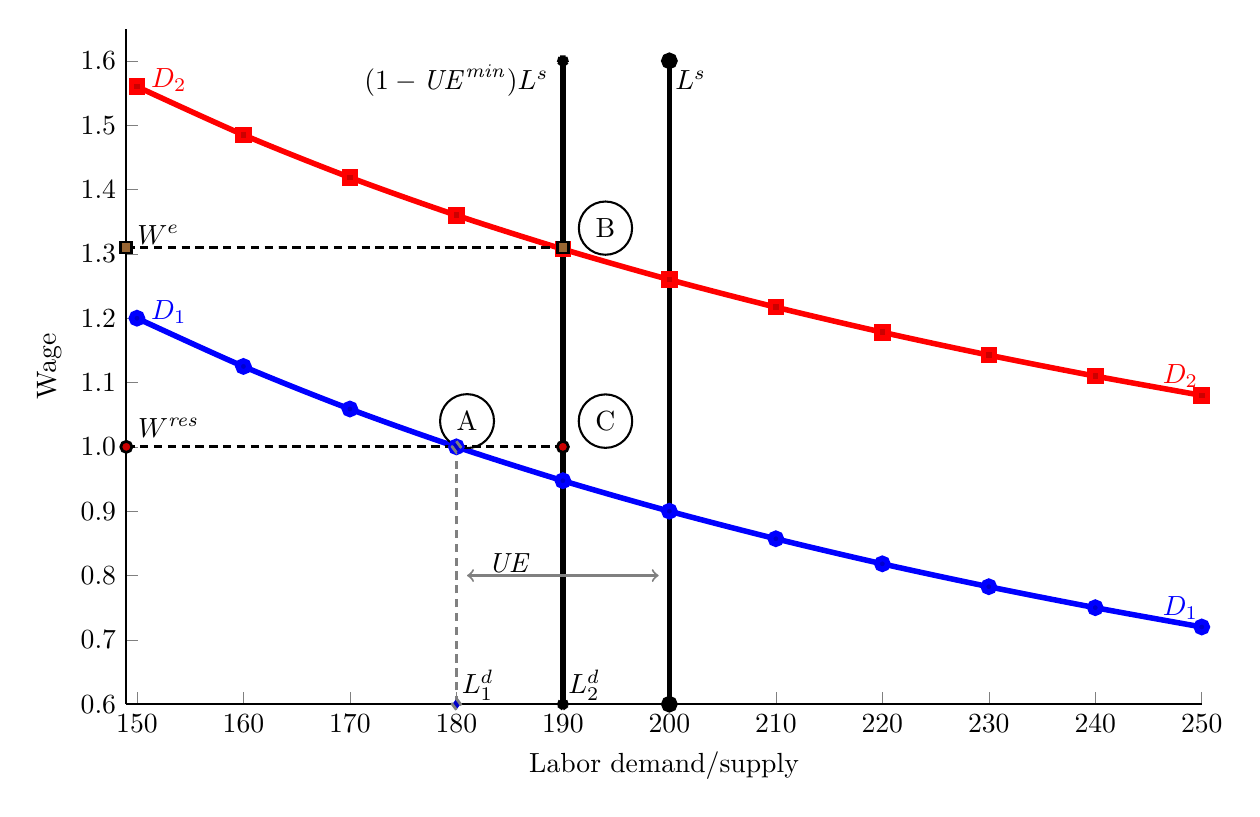
\begin{tikzpicture}
   \begin{axis}[width=6in, height=4in,
      xlabel={Labor demand/supply},
      ylabel={Wage},
      xmin={149},
      xmax={250},
      ymin={0.6},
      ymax={1.65},
      % ymajorgrids,
      legend style={draw=none},
      x tick label style={/pgf/number format/.cd, scaled x ticks = false,
         set thousands separator={},fixed},
      y tick label style={/pgf/number format/.cd, scaled y ticks = false,
         set decimal separator={.},fixed,fixed zerofill,precision=1},
      xtick={150,160,...,250},
      ytick={0.6,0.7,...,1.6},
      % legend style={at={(1.03,0.5)},anchor=west,font=\footnotesize},
      % legend cell align=left
   ]
   \addplot+[blue,smooth,line width=2.0pt] coordinates {
      (150,1.2)
      (160,1.125)
      (170,1.05882352941176)
      (180,1)
      (190,0.947368421052632)
      (200,0.9)
      (210,0.857142857142857)
      (220,0.818181818181818)
      (230,0.782608695652174)
      (240,0.75)
      (250,0.72)
   };
   \addplot+[red,smooth,line width=2.0pt] coordinates {
      (150,1.56)
      (160,1.485)
      (170,1.41882352941176)
      (180,1.36)
      (190,1.30736842105263)
      (200,1.26)
      (210,1.21714285714286)
      (220,1.17818181818182)
      (230,1.14260869565217)
      (240,1.11)
      (250,1.08)
   };
   \addplot+[black,smooth,line width=2.0pt] coordinates {
      (200,0.6)
      (200,1.6)
   };
   \addplot+[black,smooth,line width=2.0pt] coordinates {
      (190,0.6)
      (190,1.6)
   };
   \addplot+[gray,densely dashed,line width=1.0pt] coordinates {
      (180,0.6)
      (180,1.0)
   };
   \addplot+[black,smooth,line width=1.0pt] coordinates {
      (149,1.0)
      (190,1.0)
   };
   \addplot+[black,smooth,line width=1.0pt] coordinates {
      (149,1.31)
      (190,1.31)
   };
   \node[color=black] at (axis cs:202,1.57) {$L^s$};
   \node[color=black] at (axis cs:180,1.57) {$(1-\mathit{UE}^{\mathit{min}})L^s$};
   %\node[fill=white,draw] at (0,0) {$y (0,0)$};
   \node[color=black] at (axis cs:152,1.33) {$W^e$};
   \node[color=black] at (axis cs:153,1.03) {$W^{\mathit{res}}$};
   \node[color=black] at (axis cs:182,0.63) {$L^d_1$};
   \node[color=black] at (axis cs:192,0.63) {$L^d_2$};
   \node[color=blue] at (axis cs:153,1.21) {$D_1$};
   \node[color=blue] at (axis cs:248,0.75) {$D_1$};
   \node[color=red] at (axis cs:153,1.57) {$D_2$};
   \node[color=red] at (axis cs:248,1.11) {$D_2$};
   %\draw[<->,gray,densely dashed] (axis cs:181,0.8) -- (199,0.8);
   \draw[<->,color=gray] (axis cs:181,0.8) -- (axis cs:199,0.8);
   \node[color=black] at (axis cs:185,0.82) {$\mathit{UE}$};
   %\node[blue] at (axis cs:181,1.03) {A};
   \node[draw,circle,color=black] at (axis cs:181,1.04) {A};
   \node[draw,circle,color=black] at (axis cs:194,1.34) {B};
   \node[draw,circle,color=black] at (axis cs:194,1.04) {C};
   \end{axis}
   \end{tikzpicture}
\caption{{Labor market closure}}
\label{fig:LabMarket}
\end{figure}

Equation~(\ref{eq:reswage}) defines the reservation wage,
$\mathit{W}^{\mathit{res}}$. It is a positive function of income growth per
capita and the CPI. It is a negative function of the unemployment rate, i.e.
if the rate of unemployment increases, this would tend to have a downward
pressure on the reservation wage. The (positive) elasticities
$\omega^{\mathit{rwg}}$ and $\omega^{\mathit{rwp}}$ reflect the sensitivity of
the reservation wage with respect to income growth and the CPI, respectively.
The (positive) elasticity $\omega^{\mathit{rwue}}$ reflects the sensitivity of
the reservation wage with respect to the rate of unemployment.\footnote{To deal
with the possibility of zero unemployment, i.e. full employment, the reservation
wage equation is formulated in terms of changes to 1 minus the unemployment
rate, i.e. the rate of employment. The elasticity in this case should be
positive, i.e. as we approach full employment, the reservation wage is likely to
increase. The respective elasticities are linked by the formula:
$\eta=-\omega\left(1-\mathit{UE}\right)/\mathit{UE}$, where $\omega$ is the
elasticity with respect to the unemployment rate and $\eta$ is the elasticity
with respect to the employment rate. Note that this relation is not constant and
depends on the rate of unemployment. For example, if the elasticity between the
reservation wage and the unemployment rate is -0.5 and the initial unemployment
rate is 10~percent, the elasticity with respect to the employment rate is 4.5
($=-(-0.5)\cdot 0.9/0.1$).} The market wage, $W^e$ is determined by
equation~(\ref{eq:ewagez}) reflecting the complementarity condition as the
expression uses the '\texttt{=g=}' relational operator of GAMS. This equation
will be paired with the complementarity condition on the unemployment level.
Equation~(\ref{eq:uez}) defines the unemployment level.

\begin{equation}
\label{eq:reswage}
\mathit{W}^{\mathit{res}}_{r,l,z,t} =
   \chi^{rw}_{r,l,z}
   \left( 1 + g^y_{r,t}
   \right)^{\omega^{\mathit{rwg}}_{r,l,z}}
   \left( {\mathit{1-UE}^z_{r,l,z,t}}
   \right)^{\omega^{\mathit{rwue}}_{r,l,z}}
   \left( \frac {\mathit{PFD}_{r,h,t}} {\mathit{PFD}_{r,h,t-1}}
   \right)^{\omega^{\mathit{rwp}}_{r,l,z}}
\end{equation}

\begin{equation}
\label{eq:ewagez}
\mathit{W}^e_{r,l,z,t} \ge
   \mathit{W}^{\mathit{res}}_{r,l,z,t}
   \perp \mathit{UE}^z_{r,l,z,t} \ge \mathit{UEMin}^z_{r,l,z,t}
\end{equation}

\subsubsection{Monash-style labor market closure}

Equation~(\ref{eq:monashUE}) defines the motion equation
for the real wage, $\mathit{RW}$, where the superscript
$b$ refers to the baseline levels.\footnote{N.B. There is
a subtle difference with the original Monash formulation. In \textsc{Envisage}, the
equation is specified for each labor type, $l$ (and potentially
for each zone). In Monash, the equation holds for aggregate labor
demand. Wages by skill and sector are given as a proportion of the
prevailing wage.} The baseline scenario is used
to calibrate real wages and full employment is assumed.
In shock scenarios, both the real wage and labor demand
may deviate from baseline values in the short-run.
The parameter $\chi^l$ determines the speed of adjustment
back to baseline employment levels. In the standard
specification, $\eta^l$ is set to zero implying that
there is no permanent deviation from the baseline
employment level.\footnote{\cite{DixonRimmer2002} argue that,
at least in the case of Australia, this parameter ranges
from 0 to 0.15 and typically set the parameter to 0.}
The residual term can be used to shift the real wage
formulation---\cite{DixonRimmer2002} use this term to
smooth out cycles in the real wage as it converges
towards its long-term path.

\begin{equation}
\label{eq:monashUE}
\left[\frac{\mathit{RW}_{r,l,z,t}}{\mathit{RW}^b_{r,l,z,t}} - 1\right]
= \left[\frac{\mathit{RW}_{r,l,z,t-1}}{\mathit{RW}^b_{r,l,z,t-1}} - 1\right] + \chi^l_{r,l,z,t}
\left[\frac{\mathit{LD}^z_{r,l,z,t}}{\mathit{LD}^{z,b}_{r,l,z}} -
\left( \frac{\mathit{RW}_{r,l,z,t-1}}{\mathit{RW}^b_{r,l,z,t-1}}\right)^{\eta^l_{r,l,z}}\right] + \varepsilon^w_{r,l,z,t}
\end{equation}

Equation~(\ref{eq:uez}) holds for all model specifications. In the case of full-employment, $\mathit{UE}^z$ is
exogenous and this equation in effect is the equilibrium equation that determines the equilibrium wage rate.
This also holds for the Monash closure for the baseline. It could also hold for the baseline for the reservation
wage closure, where trend unemployment is fixed. In this case, the shifter on the reservation wage equation, $\chi^{rw}$,
is endogenous. In policy simulations, the shifter is fixed and unemployment is endogenous.
For the Monash closure, equation~(\ref{eq:monashUE}) is normally only active for policy simulations---though
it could also be active for other closures with the residual term, $\varepsilon^w$, then endogenous.

\begin{equation}
\label{eq:uez}
\left( 1 - \mathit{UE}^z_{r,l,z,t} \right) \mathit{LS}^z_{r,l,z,t}
   = \mathit{LD}^z_{r,l,z,t}
\end{equation}

The model allows for inter-sectoral wage differentials. These are represented by
the $\pi^w$ parameters that are calibrated using base year wage differentials
and held fixed afterwards. This implies that all wages (for a particular skill
and within a zone) move proportionately but allowing for wage differentials.
Note that this assumption has potential implications for model results as any
inter-sectoral shifts in labor may imply shifts in aggregate labor productivity
(irrespective of technological change). Equation~(\ref{eq:wage}) sets the
sectoral wage equal to the equilibrium wage (by zone) adjusted by the
sector-specific wage differential.

\begin{equation}
\label{eq:wage}
\begin{array}{*{20}{l}}
\mathit{PF}_{r,l,a} = \pi^w_{r,l,a} W^e_{r,l,z} & \textrm{for } a \in z
\end{array}
\end{equation}

If the rural to urban migration module is active, it depends on the so-called
urban premium, i.e. the extent to which the urban wage exceeds the rural wage.
Equation~(\ref{eq:awagez}) defines the average wage in each of the zones, $W^a$
(by skill). Equation~(\ref{eq:urbPrem}) defines the urban premium,
$\pi^{\mathit{Urb}}$. It is the ratio of the expected urban wage to the expected
rural wage, where the actual average wage is adjusted by the probability of
employment. Migration, which will be a function of the urban premium, is
described below as part of the dynamics of the model. In the comparative static
version of the model, it is assumed that labor supply is fixed (by zone).

\begin{equation}
\label{eq:awagez}
\mathit{W}^a_{r,l,z} =
   \frac{ \sum_{a \in z} {\mathit{PF}_{r,l,a} \mathit{XF}_{r,l,a} } }
        { \sum_{a \in z} {\mathit{XF}_{r,l,a} } }
\end{equation}

\begin{equation}
\label{eq:urbPrem}
\pi^{\mathit{Urb}}_{r,l} =
   \frac { \left( 1 - \mathit{UE}^z_{r,l,\mathit{Urb}} \right)
            W^a_{r,l,\mathit{Urb}}}
         {\left( 1 - \mathit{UE}^z_{r,l,\mathit{Rur}}\right)
            W^a_{r,l,\mathit{Rur}}}
\end{equation}

Another potentially useful concept is the notion of the skill premium, i.e. the
extent to which skilled wages exceed unskilled wages.\footnote{In a dynamic
calibration scenario, assumptions regarding the evolution of the skill premium
can be used to calibrate the relative growth of skilled vs. unskilled labor or
to calibrate productivity differentials across skills.}
Equation~(\ref{eq:twage}) defines the average economy-wide wage for each skill
type, $W^t$.\footnote{In the case of non-segmented markets, $W^t_{r,l}$ should
be equal to $W^a_{r,l,\mathit{nsg}}$.} Equation~(\ref{eq:skillprem}) defines the
so-called skill premium,  $\pi^s$. It is the percentage by which the reference
wage exceeds other wages, where the reference wage is equal to a weighted
average of wages over a subset of labor skills (where the subset is indexed by
$\mathit{lr}$)---the subset is typically the set of skilled labor types.

\begin{equation}
\label{eq:twage}
W^t_{r,l} =
   \displaystyle \frac{\sum_{a}{\mathit{PF}_{r,l,a} \mathit{XF}_{r,l,a}}}
      {\sum_{a}{\mathit{XF}_{r,l,a}}}
\end{equation}

\begin{equation}
\label{eq:skillprem}
\pi^s_{r,l,t} =
   \frac {  \sum_{\mathit{lr}} {
               W^t_{r,\mathit{lr},t}\mathit{LAB}^s_{r,\mathit{lr},t}
            }
   /  \sum_{\mathit{lr}} {
         \mathit{LAB}^s_{r,\mathit{lr},t}
      } } {W^t_{r,\mathit{l},t} } - 1
\end{equation}

The final two sets of equations define the total labor supply by skill,
equation~(\ref{eq:labseq}), and the total labor supply,
equation~(\ref{eq:tlabeq}), respectively, $\mathit{L}^s$ and $\mathit{TL}^s$. In
comparative static simulations, $\mathit{LS}^z$ is fixed by zone. In dynamic
simulations, $\mathit{LS}^z$ grows at some 'natural' rate of growth, but may
also be adjusted by rural to urban migration. This is further described below.

\begin{equation}
\label{eq:labseq}
\mathit{L}^s_{r,l} = \sum_z{\mathit{LS}^z_{r,l,z}}
\end{equation}

\begin{equation}
\label{eq:tlabeq}
\mathit{TL}^s_{r} = \sum_l{\mathit{L}^s_{r,l}}
\end{equation}

\subsection{Capital market}

The model can operate in recursive dynamic mode or in comparative static mode.
Capital market closure differs in each. In the comparative static mode, there
is a single vintage and aggregate capital is allocated across activities using
a CET transformation function. The latter allows two extreme assumptions---fixed
capital per activity, i.e. no mobility, and perfect mobility and a uniform rates
of return across activities. In dynamic mode, with vintage capital, \emph{New}
capital is fully mobile across sectors. \emph{Old} capital is released on the
secondary capital market if installed capital exceeds demand, for example in
declining sectors.

\subsubsection{Comparative static closure}

A CET transformation function is used to allocate aggregate capital in the
comparative static version of the model. Equation~(\ref{eq:kscs}) describes the
supply of capital to activity $a$, $K^s$, where $\omega^k$ determines the degree
of mobility across activities.\footnote{The vintage index is for convenience
only. In the comparative static version there is only a single vintage.} With
perfect mobility, the rate of return across activities is uniform.
Equation~(\ref{eq:trcs}) determines the aggregate rate of return to capital,
$\mathit{TR}$. Equation~(\ref{eq:pkcs}) is the equilibrium condition for
capital---supply of capital to each activity is equal to demand. In the model
implementation the equilibrium condition is substituted out.

\begin{equation}
\label{eq:kscs}
\begin{cases}
\displaystyle K^s_{r,a,v} =
   \gamma^k_{r,a,v}
   \left( \frac{\mathit{PK}_{r,a,v}} {\mathit{TR}_r}
   \right)^{\omega^k_r}
   \mathit{TK}^s_r
& \textrm{if } \omega^k_{r} \ne \infty \\
\displaystyle \mathit{PK}_{r,a,v} =
   \mathit{TR}_r
& \textrm{if } \omega^k_{r} = \infty \\
\end{cases}
\end{equation}

\begin{equation}
\label{eq:trcs}
\mathit{TR}_r \mathit{TK}^s_r =
   \sum_a {\sum_v {\mathit{PK}_{r,a,v} K^s_{r,a,v} } }
\end{equation}

\begin{equation}
\label{eq:pkcs}
K^s_{r,a,v} = K^v_{r,a,v}
\end{equation}

\subsubsection{Vintage capital closure}

There are two types of capital in the vintage specification, \emph{Old}, or installed
capital, and \emph{New} capital. Initial installed capital is set at the beginning of the period
and is equal to the depreciated level of the previous period's aggregation of
both \emph{Old} and \emph{New} capital. The demand for \emph{New} capital will
depend on market conditions, substitution and other factors. A sector
is in expansion if demand for \emph{New} capital exceeds the initial
installed capital. A sector is in contraction if demand for capital in the
sector is less than its initial installed capital. This can come about, for example,
if public policies affect demand for a good---such as a carbon tax leading
to reduced demand for coal or oil. If a sector is in contraction, it will
release its \emph{Old} capital using an upward sloping supply schedule, potentially
with an infinite elasticity.

Figure~\ref{fig:kSupply} represents the two
possible regimes each under two possible capital demand schedules. The
left panel shows the case for a flat supply curve, i.e. an infinite
supply curve for \emph{Old} capital. In that case, even if capital
demand is contracting, the rate of return to \emph{Old} capital
is equated to the economy-wide rental rate, i.e. the ratio of
returns, \emph{Old} over \emph{New} is 1. The right panel shows
the case where the supply of \emph{Old} capital follows an upward
sloping schedule. If capital demand is in decline, the rate
of return to \emph{Old} capital will be less than the economy-wide
return. In the case of an expanding demand, the rate of return
to \emph{Old} capital is equal to the economy-wide return and
the supply of \emph{Old} capital is capped at the initially installed
level, i.e. $K_0$.

\begin{figure}[ht]
	\centering
	\subfloat[][\scriptsize{$\eta^I = \infty$}]{
		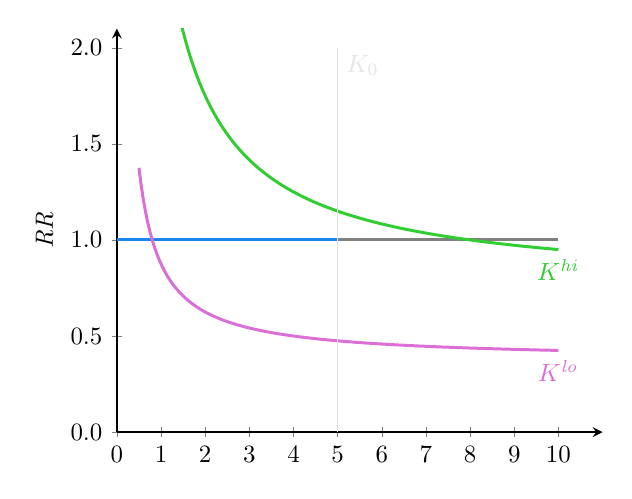
\begin{tikzpicture}[scale=0.9]
		\begin{axis}[axis x line=bottom, axis y line=left, 
		xtick={0,1,...,10}, ytick={0.0,0.5,...,2.0}, xmax=11, ymin=0, ymax=2.1, ylabel=$\mathit{RR}$,
		y tick label style={/pgf/number format/.cd,fixed,fixed zerofill,precision=1,/tikz/.cd}]
		\addplot[DodgerBlue2,very thick,mark=none,domain=0:5,samples=100]
		{0.5*(1+(5/5)^1.5)};
		\addplot[gray,very thick,mark=none,domain=5:10,samples=100]
		{0.5*(1+(5/5)^1.5)} ;
		\addplot[Orchid,very thick,mark=none,domain=0.5:10,samples=200]
		{0.5*((\x/1)^(-1/1)+0.75)} node[below] {$K^{\mathit{lo}}$};
		\addplot[LimeGreen,very thick,mark=none,domain=1:10,samples=200]
		{0.5*((\x/4)^(-1/1)+1.5)} node[below] {$K^{\mathit{hi}}$};
		\addplot[lightgray,thin,mark=none]
		coordinates{(5,0) (5,2.0)} node[right,yshift=-0.25cm] {$K_{0}$} ;
		%\addplot[Orchid,thin,dashed,mark=none]
		%coordinates{(11.6,0) (11.6,1)} ;
		\end{axis}
		\end{tikzpicture}
	} \qquad
	\subfloat[][\scriptsize{$\eta^{\mathit{I}} \ne \infty$}]{
		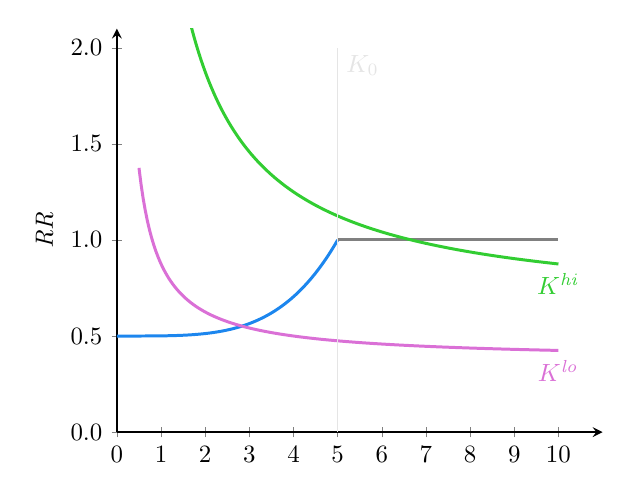
\begin{tikzpicture}[scale=0.9]
		\begin{axis}[axis x line=bottom, axis y line=left, 
		xtick={0,1,...,10}, ytick={0.0,0.5,...,2.5}, xmax=11, ymin=0, ymax=2.1, ylabel=$\mathit{RR}$,
		y tick label style={/pgf/number format/.cd,fixed,fixed zerofill,precision=1,/tikz/.cd}]
		\addplot[DodgerBlue2,very thick,mark=none,domain=0:5,samples=100]
		{0.5*(1+(\x/5)^4)};
		\addplot[gray,very thick,mark=none,domain=5:10,samples=100]
		{0.5*(1+(5/5)^1.5)};
		\addplot[Orchid,very thick,mark=none,domain=0.5:10,samples=200]
		{0.5*((\x/1)^(-1/1)+0.75)} node[below] {$K^{\mathit{lo}}$};
		\addplot[LimeGreen,very thick,mark=none,domain=1:10,samples=200]
		{0.5*((\x/5)^(-1/1)+1.25)} node[below] {$K^{\mathit{hi}}$};
		\addplot[lightgray,thin,mark=none]
		coordinates{(5,0) (5,2.0)} node[right,yshift=-0.25cm] {$K_{0}$} ;
		%\addplot[Orchid,thin,dashed,mark=none]
		%coordinates{(11.6,0) (11.6,1)} ;
		\end{axis}
		\end{tikzpicture}
	} \\
	\caption{Capital supply regimes}
	\label{fig:kSupply}
\end{figure}


Equation~(\ref{eq:kslo}) represents the mixed complementarity
condition for the supply of old capital. If demand is contracting,
the upward sloping portion of the supply schedule is determined
by the iso-elastic relation with the supply elasticity given
by $\eta^I$. At the inflection point, the supply of \emph{Old}
capital cannot exceed the amount of the initially installed \emph{Old}
given by $K^0$. The complementarity condition then translates into:
(a) all of the installed capital is needed, $K^{\mathit{lo}}=K^0$ and the ratio
of returns is equal to 1; or (b) the supply of old capital
is less than the installed capital and the ratio of returns is
less than 1. The second complementarity condition, equation~(\ref{eq:rrat}),
states that either the ratio of returns is 1 and thus supply of new
capital is positive, or the ratio is less than 1 and then the supply of new
capital is 0. Equation~(\ref{eq:kshi}) states that total supply
should meet total demand. The model allows for the possibility
of a horizontal supply schedule, in which case the ratio of returns
is equal to 1 irrespective of market conditions and supply will be
set to demand.

\begin{equation}
\label{eq:kslo}
K^{\mathit{lo}}_{r,a} \ge \mathit{K}^0_{r,a} \mathit{RR}_{r,a}^{\eta^I_{r,a}}
\perp \mathit{RR}_{r,a} \le 1
\end{equation}

\begin{equation}
\label{eq:rrat}
\mathit{RR}_{r,a} \le 1
\perp K^{\mathit{hi}}_{r,a} \ge 0
\end{equation}

\begin{equation}
\label{eq:kshi}
K^{\mathit{lo}}_{r,a} + K^{\mathit{hi}}_{r,a} = \sum_v{K^v_{r,a,v}}
\end{equation}

Equation~(\ref{eq:tr}) determines the economy-wide rate of return,
$\mathit{TR}$. Equation~(\ref{eq:pk}) determines the sector- and
vintage-specific rate of return. If the activity uses \emph{New} capital,
$\mathit{RR}$ is equal to 1 and both \emph{Old} and \emph{New} capital obtain
the rate of return $\mathit{TR}$. If the sector is in decline, it receives a
rate of return lower than the economy-wide rate of return.

\begin{equation}
\label{eq:tr}
\mathit{TK}^s_r = \sum_a {\sum_v { K^v_{r,a,v}} }
\end{equation}

\begin{equation}
\label{eq:pk}
\mathit{PK}_{r,a,v} = \mathit{RR}_{r,a} \mathit{TR}_r
\end{equation}

\subsubsection{Determination of output by vintage}

Aggregate output, $\mathit{XP}$, is determined by equilibrium conditions.
Equation~(\ref{eq:kxrat}) represents the contemporaneous capital-output ratio
for the \emph{Old} vintage, $\mathit{kxRat}$. Equation~(\ref{eq:xpvold}) determines output with \emph{Old} capital. \emph{Old} output, will be equal to the
capital output ratio applied to the supply of old
capital, $K^{\mathit{lo}}$. Equation~(\ref{eq:xpv}) ensures that the sum
of output across vintages equals aggregate output. In the vintage capital
version of the model, it essentially determines production with \emph{New}
capital. In the comparative static version, it trivially equates total
production to production produced by the only vintage that is labeled
\emph{Old}.

\begin{equation}
\label{eq:kxrat}
\mathit{kxRat}_{r,a,\mathit{Old}} =
   \frac {K^v_{r,a,\mathit{Old}}} {\mathit{XPv}_{r,a,\mathit{Old}}}
\end{equation}

\begin{equation}
\label{eq:xpvold}
\mathit{kxRat}_{r,a,\mathit{Old}} \mathit{XPv}_{r,a,\mathit{Old}} =
K^{\mathit{lo}}_{r,a}
\end{equation}

\begin{equation}
\label{eq:xpv}
\mathit{XP}_{r,a} = \sum_v{ \mathit{XPv}_{r,a,v}}
\end{equation}

Equations~(\ref{eq:xfcap}) and~(\ref{eq:pfcap}) are added for accounting
purposes as many of the various income identities are simplified with these
substitutions. Equation~(\ref{eq:pfcap}) holds in all circumstances. If an
activity is expanding the return on installed capital is equal to the return on
\emph{New} capital. If an activity is contracting, the only relevant return is
on \emph{Old} capital.

\begin{equation}
\label{eq:xfcap}
\mathit{XF}_{r,cap,a} = \sum_v{ \mathit{K}^v_{r,a,v}}
\end{equation}

\begin{equation}
\label{eq:pfcap}
\mathit{PF}_{r,cap,a} = \mathit{PK}_{r,a,\mathit{Old}}
\end{equation}

\subsection{Land market}

The supply side of the land market has two components. The first component
provides the aggregate supply of land, by land-type.\footnote{[20-Apr-2022]
The code has been modified to allow for multiple land types, for example
AEZs. The specification for land supply is identical to the previous
version except that all relevant equations and variables are now
indexed by land type, i.e., $\mathit{lnd}$. With the default GTAP
database, there is a single land-type. With GTAP's AEZ database, there
can be up to 18 land-types for each land-using activity in each region.}
The second step allocates aggregate land by type
across different activities allowing for a nested CET structure, the possibility
of perfect mobility, and the use of the adjusted CET that preserves land
additivity.

The aggregate land supply curve is allowed to have four shapes---constant
elasticity, a logistic curve with an upward asymptote, a generalized hyperbola
also with an upward asymptote, and perfectly horizontal. The aggregate land
supply curve is given by equation~(\ref{eq:tland}). The initial elasticity of
aggregate land is given by $\eta^t$.

\begin{equation}
\label{eq:tland}
\begin{cases}
   \displaystyle \mathit{TLand}_{r,\mathit{lnd}} =
      \chi^t_{r,\mathit{lnd}} \left( \frac{\mathit{PTLand}_{r,\mathit{lnd}}} {\mathit{PGDP}_r}
      \right)^{\eta^t_{r,\mathit{lnd}}}
   & \textrm{iso-elastic} \\
   \displaystyle \mathit{TLand}_{r,\mathit{lnd}} =
      \frac {\mathit{TLand}^{\mathit{Max}}_{r,\mathit{lnd}}}
            {1 + \chi^t_{r,\mathit{lnd}} e^{-\gamma^{\mathit{tl}}_{r,\mathit{lnd}}
               (\mathit{PTLand}_{r,\mathit{lnd}}/\mathit{PGDP}_r)}}
   & \textrm{logistic} \\
   \displaystyle \mathit{TLand}_{r,\mathit{lnd}} =
      {\mathit{TLand}^{\mathit{Max}}_{r,\mathit{lnd}}} {- \chi^t_{r,\mathit{lnd}}
      \left( \frac{\mathit{PTLand}_{r,\mathit{lnd}}} {\mathit{PGDP}_r}
      \right)^{-\gamma^{\mathit{tl}}_{r,\mathit{lnd}}}}
   & \textrm{hyperbola} \\
   \displaystyle \mathit{PTLand}_{r,\mathit{lnd}} = \mathit{PGDP}_{r,\mathit{lnd}}
   & \textrm{if } \eta^t_{r,\mathit{lnd}} = \infty \\
\end{cases}
\end{equation}

The iso-elastic curve by definition has a constant elasticity given by $\eta^t$.
The logistic function, in a simplified form is given by:

\[
S=\frac {\overbar{S}} {1+\chi e^{-\gamma P}}
\]

\noindent where $S$ is supply, the land maximum is given by $\overbar{S}$ and
$P$ is the real price of land. The supply elasticity is given by the following
formula:

\[
\eta = \gamma P \left( \frac {\overbar{S}-S}{\overbar{S}} \right)
\]

\noindent The $\gamma$ coefficient can be calibrated using the expression above
given initial values for $\eta$, $S$, $\overbar{S}$ and $P$. The calibration
formula is given by:

\[
\gamma = \frac{\eta} {P} \left( \frac {\overbar{S}} {\overbar{S}-S} \right)
\]

\noindent Calibration of the $\chi$ parameter is given by the following
expression and requires first calibrating the $\gamma$ parameter:

\[
\chi = e^{\gamma P} \left( \frac {\overbar{S}-S}{\overbar{S}} \right)
\]

The generalized hyperbola, using the same notation is given by:

\[
S= \overbar{S} - \chi P^{-\gamma}
\]

\noindent The supply elasticity is given by the following formula:

\[
\eta = \gamma \left( \frac {\overbar{S}-S}{{S}} \right)
\]

\noindent The $\gamma$ coefficient can be calibrated using the expression above
given initial values for $\eta$, $S$, $\overbar{S}$ and $P$. The calibration
formula is given by:

\[
\gamma = {\eta} \left( \frac {{S}} {\overbar{S}-S} \right)
\]

\noindent Calibration of the $\chi$ parameter is given by the following
expression and requires first calibrating the $\gamma$ parameter:

\[
\chi = P^\gamma \left( \overbar{S}-S \right)
\]

The user chooses the functional form by setting the global parameter named
\texttt{TASS} towards the top of a simulation file. Valid options are
\texttt{KELAS} for the iso-elastic form, \texttt{LOGIST} for the logistic
specification, \texttt{HYPERB} for the generalized hyperbola and \texttt{INFTY}
for the horizontal supply function.\footnote{These options are defined in the
\texttt{model.gms} file with a set named \texttt{landAssumptions}. The subset
named \texttt{tass} contains the user-chosen specification.}

Total land is allocated across different uses according to the relative rates of
return across uses. A nested CET structure is implemented that allows for a
degree of user control.\footnote{The implementation was first developed to mimic
the CET structure of the land allocation specification in the MAGNET model.}
Figure~\ref{fig:LandNest} provides a graphic depiction of the land allocation
specification. The number of land bundles ($\mathit{XLB}$) is under user
control, but typically there should be at least one. The first land bundle is in
the top CET nest with an intermediate land bundle ($\mathit{XLB}$). All other
land bundles are nested within the intermediate land bundle. Some possible
configurations from the literature include:

\begin{itemize}
\item{To mimic
MAGNET's specification, \texttt{v\_f}, \texttt{ocr}, \texttt{oap} are mapped
to land bundle 1, \texttt{sug}, \texttt{ctl} and \texttt{rmk} are mapped to land
bundle 2 and \texttt{ric}, \texttt{wht}, \texttt{gro} and \texttt{osd} are
mapped to land bundle 2. The MAGNET model has two intermediate bundles and only
three elasticities. In this specification, there are four intermediate bundles.
Thus the top elasticity and the elasticity for land bundle 1
(horticulture, etc.), in MAGNET, are identical (and set to $\sigma^1$ in the
MAGNET documentation, see \url{edepot.wur.nl/310764}, page 74).
The elasticity
for the intermediate land bundle and the second land bundle (pasture, etc.)
would also be identical (and set to $\sigma^2$). And the third land bundle
(cereals) would have the elasticity given by $\sigma^3$.}
\item{The original version of the GTAP-AEZ model, \citep{HerteletalChap62009}
has forestry in land bundle 1. The intermediate bundle is called
agriculture---under which there are two additional bundles: crops
and grazing. All crops are then assigned to the \emph{Crops} bundle
and all livestock activities are assigned to the \emph{Grazing} bundle.\footnote{That
version of the GTAP-AEZ model had a fixed aggregation for grazing that
included cattle (\texttt{ctl}), raw milk (\texttt{rmk}) and wool (\texttt{wol}).}
The AEZ-based land-use database removes land-use from the \texttt{oap} sector.}
\item{A different version of the GTAP-AEZ model has altered the
original nesting. It has crops in bundle 1, and a grazing plus forestry
bundle as the intermediate bundle \citep{StevensonetalPNAS2013}.}
\end{itemize}

It is possible to
mimic the GTAP standard nesting, a single level nest, by defining only one land
bundle and use the GTAP transformation elasticity for that bundle. The top level
elasticity is essentially irrelevant since in this case the intermediate land
bundle would not be used.

\begin{figure}[ht]
\center{}
\begin{forest}
for tree={
   minimum height=1cm,
   font=\tiny,
%  font=\sffamily,
   anchor=north,
   align=center,
   child anchor=north,
   s sep=1em,
   l sep=0.75cm,
},
%where n children=0{tier=word}{}
[{Total land \\ supply ($\mathit{TLand}_{\mathit{lnd}}$)}, draw, drop shadow, fill=dkBlue, rounded corners=2pt, name=TLAND
   [{Land bundle(1) \\  ($\mathit{XLB}_{\mathit{lnd},\mathit{lb1}}$)}, draw, drop shadow, fill=mdBlue, rounded corners=2pt, name=XLB1
   [][$\mathit{XF}_{\mathit{lnd},a} \in \mathit{XLB}_{\mathit{lnd},\mathit{lb1}}$, draw, drop shadow, fill=ltBlue, rounded corners=2pt][]
   ]
   [{Demand for intermediate \\ land bundle ($\mathit{XNLB}_{\mathit{lnd}}$)}, draw, drop shadow, fill=mdBlue, rounded corners=2pt, name=XNLB
      [{Land bundle(2) \\ ($\mathit{XLB}_{\mathit{lnd},\mathit{lb2}}$)}, draw, drop shadow, fill=mdBlue, rounded corners=2pt, name=XLB2
      [][$\mathit{XF}_{\mathit{lnd},\mathit{lnd},a} \in \mathit{XLB}_{\mathit{lnd},\mathit{lb2}}$, draw, drop shadow, fill=ltBlue, rounded corners=2pt][]
      ]
      [{Land bundle(3) \\ ($\mathit{XLB}_{\mathit{lnd},\mathit{lb3}}$)}, draw, drop shadow, fill=mdBlue, rounded corners=2pt, name=XLB3
      [][$\mathit{XF}_{\mathit{lnd},a} \in \mathit{XLB}_{\mathit{lnd},\mathit{lb3}}$, draw, drop shadow, fill=ltBlue, rounded corners=2pt][]
      ]
      [{Land bundle($n$) \\ ($\mathit{XLB}_{\mathit{lnd},\mathit{lbn}}$)}, draw, drop shadow, fill=mdBlue, rounded corners=2pt, name=XLBN
      [][$\mathit{XF}_{\mathit{lnd},a} \in \mathit{XLB}_{\mathit{lnd},\mathit{lbn}}$, draw, drop shadow, fill=ltBlue, rounded corners=2pt][]
      ]
   ]
]
\node[anchor=west,align=left]
  at ([yshift=-0.35cm,xshift=-0.45cm]TLAND.south) {\scriptsize $\omega^{\mathit{t}}$};
\node[anchor=west,align=left]
  at ([yshift=-0.35cm,xshift=-0.05cm]XLB1.south) {\scriptsize $\omega^{\mathit{lb1}}$};
\node[anchor=west,align=left]
  at ([yshift=-0.35cm,xshift=-0.05cm]XNLB.south) {\scriptsize $\omega^{\mathit{nlb}}$};
\node[anchor=west,align=left]
  at ([yshift=-0.35cm,xshift=-0.05cm]XLB2.south) {\scriptsize $\omega^{\mathit{lb2}}$};
\node[anchor=west,align=left]
  at ([yshift=-0.35cm,xshift=-0.05cm]XLB3.south) {\scriptsize $\omega^{\mathit{lb3}}$};
\node[anchor=west,align=left]
  at ([yshift=-0.35cm,xshift=-0.05cm]XLBN.south) {\scriptsize $\omega^{\mathit{lbn}}$};
%{\draw[white,dotted] (!1) -| coordinate(p) () ;
%\path ()--(p) node[pos=0.1,left,inner sep=1pt]{\scriptsize $\sigma^p$};}
\end{forest}
\caption{{CET nest for land allocation across activities by land-type}}
\label{fig:LandNest}
\end{figure}

The top level nest decomposes total land supply into land bundle 1 and the
intermediate land bundle. Equations~(\ref{eq:lb1}) and~(\ref{eq:nlb}) provide
the first order conditions and hold irrespective of the CET specification
used---either the standard, with \texttt{ifLandCET} set to 1, or the adjusted,
volume preserving, CET specification. Equation~(\ref{eq:ptlandn}) defines the
aggregate price index of land, $\mathit{PTLandN}$. The index expression depends
on the choice of CET specification. For the standard CET, the price index will
be identical to the average price (defined next). For the adjusted CET, the
price index will not generally be equal to the average price. Note that the
price index expressions are not incorporated in the model under the assumption
of perfect transformation, i.e. when the transformation elasticity is infinite.
The average price of aggregate land, $\mathit{PTLand}$ is given in
equation~(\ref{eq:ptland}) and holds for both versions of the CET.

\begin{equation}
\label{eq:lb1}
\begin{cases}
\displaystyle \mathit{XLB}_{r,\mathit{lnd},\mathit{lb1}} =
   \gamma^{\mathit{lb}}_{r,\mathit{lnd},\mathit{lb1}}
   \left( \frac{\mathit{PLB}_{r,\mathit{lnd},\mathit{lb1}}} {\mathit{PTLandN_{r,\mathit{lnd}}}}
   \right)^{\omega^t_{r,\mathit{lnd}}}
   \mathit{TLand_{r,\mathit{lnd}}}
& \textrm{if } \omega^t_{r,\mathit{lnd}} \ne \infty \\
\displaystyle \mathit{PLB}_{r,\mathit{lnd},\mathit{lb1}} = \mathit{PTLand_{r,\mathit{lnd}}}
& \textrm{if} \; \omega^t_{r,\mathit{lnd}} = \infty \\
\end{cases}
\end{equation}

\begin{equation}
\label{eq:nlb}
\begin{cases}
\displaystyle \mathit{XNLB}_{r,\mathit{lnd}} =
   \gamma^{\mathit{nlb}}_{r,\mathit{lnd}}
   \left( \frac{\mathit{PNLB}_{r,\mathit{lnd}}} {\mathit{PTLandN_{r,\mathit{lnd}}}}
   \right)^{\omega^t_{r,\mathit{lnd}}}
   \mathit{TLand_{r,\mathit{lnd}}}
&  \textrm{if} \; \omega^t_{r,\mathit{lnd}} \ne \infty \\
\displaystyle \mathit{PNLB}_{r,\mathit{lnd}} = \mathit{PTLand_{r,\mathit{lnd}}}
& \textrm{if} \; \omega^t_{r,\mathit{lnd}} = \infty \\
\end{cases}
\end{equation}

\begin{equation}
\label{eq:ptlandn}
\begin{cases}
\mathit{PTLandN_{r,\mathit{lnd}}} =
   \left[
      \gamma^{\mathit{lb}}_{r,\mathit{lnd},\mathit{lb1}}
      \mathit{PLB}_{r,\mathit{lnd},\mathit{lb1}}^{1+\omega^t_{r,\mathit{lnd}}}
   +  \gamma^{\mathit{nlb}}_{r,\mathit{lnd}}
      \mathit{PNLB}_{r,\mathit{lnd}}^{1+\omega^t_{r,\mathit{lnd}}}
   \right]^{{1}/{(1+\omega^t_{r,\mathit{lnd}})}}
& \textnormal{if } \mathit{ifLandCET} \\
\mathit{PTLandN_{r,\mathit{lnd}}} =
   \left[
      \gamma^{\mathit{lb}}_{r,\mathit{lnd},\mathit{lb1}}
      \mathit{PLB}_{r,\mathit{lnd},\mathit{lb1}}^{\omega^t_{r,\mathit{lnd}}}
   +  \gamma^{\mathit{nlb}}_{r,\mathit{lnd}}
      \mathit{PNLB}_{r,\mathit{lnd}}^{\omega^t_{r,\mathit{lnd}}}
   \right]^{{1}/{\omega^t_{r,\mathit{lnd}}}}
& \textnormal{if } \neg \mathit{ifLandCET} \\
\end{cases}
\end{equation}

\begin{equation}
\label{eq:ptland}
\mathit{PTLand_{r,\mathit{lnd}}} \mathit{TLand_{r,\mathit{lnd}}} =
   \mathit{PLB}_{r,\mathit{lnd},\mathit{lb1}} \mathit{XLB}_{r,\mathit{lnd},\mathit{lb1}}
+  \mathit{PNLB}_{r,\mathit{lnd}}\mathit{XNLB}_{r,\mathit{lnd}}
\end{equation}

The second level nest decomposes the intermediate land bundle (if it is defined)
into a number of user determined land bundles, excluding the first land bundle.
Equation~(\ref{eq:lbn}) defines the demand for the land bundles as a share of
the intermediate land bundle.\footnote{The index $\mathit{lb}$ excludes the
first land bundle.} The price index of the intermediate land bundle is defined
in equation~(\ref{eq:pnlbn}), allowing for both CET specifications and is only
included if the transformation elasticity at this nest is finite. The average
price of the land bundle is defined in equation~(\ref{eq:pnlb}).

\begin{equation}
\label{eq:lbn}
\begin{cases}
   \displaystyle \mathit{XLB}_{r,\mathit{lnd},\mathit{lb}} =
      \gamma^{\mathit{lb}}_{r,\mathit{lnd},\mathit{lb}}
      \left( \frac{\mathit{PLB}_{r,\mathit{lnd},\mathit{lb}}} {\mathit{PNLBN_{r,\mathit{lnd}}}}
      \right)^{\omega^{\mathit{nlb}}_{r,\mathit{lnd}}}
      \mathit{XNLB_{r,\mathit{lnd}}}
   & \textrm{if } \omega^{\mathit{nlb}}_{r,\mathit{lnd}} \ne \infty \\
   \displaystyle \mathit{PLB}_{r,\mathit{lnd},\mathit{lb}} = \mathit{PNLB_{r,\mathit{lnd}}}
   & \textrm{if }  \omega^{\mathit{nlb}}_{r,\mathit{lnd}} = \infty \\
\end{cases}
\end{equation}

\begin{equation}
\label{eq:pnlbn}
\begin{cases}
   \mathit{PNLBN}_{r,\mathit{lnd}} =
      \displaystyle
         \left[
            \sum_{\left\{ \mathit{lb}: \mathit{lb} \ne {\mathit{lb1}}\right\}} {
               \gamma^{\mathit{lb}}_{r,\mathit{lnd},\mathit{lb}}
               \mathit{PLB}_{r,\mathit{lnd},\mathit{lb}}^{1+\omega^{\mathit{nlb}}_{r,\mathit{lnd}}}
            }
         \right]^{{1}/{(1+\omega^{\mathit{nlb}}_{r,\mathit{lnd}})}}
      & \textrm{if} \; \mathit{ifLandCET} \\
   \mathit{PNLBN}_{r,\mathit{lnd}} =
      \displaystyle
         \left[
            \sum_{\left\{\mathit{lb}:\mathit{lb} \ne {\mathit{lb1}}\right\}} {
               \gamma^{\mathit{lb}}_{r,\mathit{lnd},\mathit{lb}}
               \mathit{PLB}_{r,\mathit{lnd},\mathit{lb}}^{\omega^{\mathit{nlb}}_{r,\mathit{lnd}}}
            }
         \right]^{{1}/{\omega^{\mathit{nlb}}_{r,\mathit{lnd}}}}
      & \textrm{if} \; \neg \mathit{ifLandCET} \\
\end{cases}
\end{equation}

\begin{equation}
\label{eq:pnlb}
\mathit{PNLB_{r,\mathit{lnd}}} \mathit{XNLB_{r,\mathit{lnd}}} =
   \sum_{\left\{ \mathit{lb}: \mathit{lb} \ne \mathit{lb1} \right\} }{
   \mathit{PLB}_{r,\mathit{lnd},\mathit{lb}} \mathit{XLB}_{r,\mathit{lnd},\mathit{lb}}}
\end{equation}

The bottom land nest(s) decompose each of the land bundles into the primary land
allocation to each activity $a$---each activity $a$ (that uses land) must be
mapped to one, and only one, land bundle. Equation~(\ref{eq:lands}) defines the
supply of land to activity $a$ that has been mapped to land bundle
$\mathit{lb}$. Equation~(\ref{eq:plbn}) defines the price index for the bundles
that depends on the CET specification. And equation~(\ref{eq:plb}) defines the
average price of the land bundles.

\begin{equation}
\label{eq:lands}
\begin{cases}
   \displaystyle \mathit{Land}^s_{r,\mathit{lnd},a} =
      \gamma^{t}_{r,\mathit{lnd},a}
      \left( \frac {\mathit{PF}_{r,\mathit{lnd},a}}
         {\mathit{PLBN}_{r,\mathit{lnd},\mathit{lb}}}
      \right)^{\omega^{\mathit{lb}}_{r,\mathit{lnd},\mathit{lb}}}
      \mathit{XLB}_{r,\mathit{lnd},\mathit{lb}}
   & \textrm{if } \omega^{\mathit{lb}}_{r,\mathit{lnd},\mathit{lb}} \ne \infty \\
   \displaystyle \mathit{PF}_{r,\mathit{lnd},a} = \mathit{PLB}_{r,\mathit{lnd},\mathit{lb}}
   & \textrm{if} \; \omega^{\mathit{lb}}_{r,\mathit{lnd},\mathit{lb}} = \infty \\
\end{cases} {a \in \left\{ \mathit{lb} \right\}}
\end{equation}

\begin{equation}
\label{eq:plbn}
\begin{cases}
   \mathit{PLBN}_{r,\mathit{lnd},\mathit{lb}} =
      \displaystyle \left[ \sum_{a \in \left\{ \mathit{lb} \right\} } {
         \gamma^{t}_{r,\mathit{lnd},a}
         \mathit{PF}_{r,\mathit{lnd},a}^{1+\omega^{\mathit{lb}}_{r,\mathit{lnd},\mathit{lb}}}
      } \right]^{{1}/{(1+\omega^{\mathit{lb}}_{r,\mathit{lnd},\mathit{lb}})}}
   & \textrm{if } \mathit{ifLandCET} \\
   \mathit{PLBN}_{r,\mathit{lnd},\mathit{lb}} =
      \displaystyle \left[ \sum_{a \in \left\{ \mathit{lb} \right\} } {
         \gamma^{t}_{r,\mathit{lnd},a}
         \mathit{PF}_{r,\mathit{lnd},a}^{\omega^{\mathit{lb}}_{r,\mathit{lnd},\mathit{lb}}}
      } \right]^{{1}/{\omega^{\mathit{lb}}_{r,\mathit{lnd},\mathit{lb}}}}
   & \textrm{if} \; \neg \mathit{ifLandCET} \\
\end{cases}
\end{equation}

\begin{equation}
\label{eq:plb}
\mathit{PLB}_{r,\mathit{lnd},\mathit{lb}} \mathit{XLB}_{r,\mathit{lnd},\mathit{lb}} =
   \displaystyle \sum_{a \in \left\{ \mathit{lb} \right\} } {
      \mathit{PF}_{r,\mathit{lnd},a} \mathit{Land}^s_{r,\mathit{lnd},a}
   }
\end{equation}

The final equation in the land market module, equation~(\ref{eq:pland}) equates
land supply to activity $a$ to its respective demand thus determining the
equilibrium and sector-specific price for land, $\mathit{PF}_{\mathit{lnd}}$.
The equation is substituted out of the model specification.

\begin{equation}
\label{eq:pland}
\mathit{Land}^s_{r,\mathit{lnd},a} = \mathit{XF}_{r,\mathit{lnd},a}
\end{equation}

\subsection{Market for natural resources}

Natural resources are assumed to be activity-specific, for example crude oil
reserves. The supply of natural resources, $\mathit{XNRS^s}$, is governed by a
kinked iso-elastic supply curve. The model allows the supply response to differ
according to whether market conditions are leading to increased supply, the 'hi'
elasticity, versus a contracting market, the 'lo' elasticity. Ideally, we could
implement this with a regime shift using continuous functions, but discontinuous
derivatives. Instead, we add an equation to the model that determines the supply
elasticity using the sigmoid function, also known as a logistic
function.\footnote{This is used for example in the CAPRI model of global
agriculture with a focus on the EU, \cite{Britzetal2007}.} The sigmoid function
is defined by:

\[
f(x) = \frac{1}{1+e^{-x}}
\]

\noindent Equation~(\ref{eq:etanrs}) defines the applied elasticity as a
function of market conditions. The user enters the 'lo' and 'hi' elasticities in
the parameters $\eta^{\mathit{nrsx}}$. One would typically assume that the 'lo'
elasticity is higher than the 'hi' elasticity, i.e. it is harder to expand
output than to contract output. If the two are identical, the equation is
trivial. The argument in the sigmoid function reflects market growth and will be
positive for expansion and negative for contraction. The $\kappa$ parameter
captures the 'speed' of adjustment between the 'lo' and 'hi' elasticities.
The greater the value, the more rapid the transition. We have used a value of 30
with few numerical problems.\footnote{The sigmoid function is an intrinsic
function in GAMS.} Figure~\ref{fig:kinkSupply} shows the kinked elasticity and
the resulting supply curve s a function of price. It is centered at a price
of~1. The 'lo' elasticity is assumed to be 2 and the 'hi' elasticity is 0.5.
The 'kink' parameter is been set at 10 in this example.

%\clearpage

\begin{figure}[ht]
\begin{minipage}{\textwidth}
\centering
   \begin{tikzpicture}[x=30mm,y=30mm]

%\draw[help lines] (0,0) grid (13,13);

\draw[->] (0,0) -- (2.7,0) node[right] {$P$};
\draw[->] (0,0) -- (0,2.7) node[right] {$Q,\eta$};

\draw[color=gray!30] (1,0) -- (1,2.5) node[right] {\color{black}{$P=1$}};
\draw[color=gray!30] (0,0.5) -- (2.5,0.5) node[below right] {\color{black}{$\eta=0.5$}};
\draw[color=gray!30] (0,2) -- (2.5,2) node[below right] {\color{black}{$\eta=2.0$}} ;

%\foreach \i in {0.5,1.0,...,2.5} {
%	\draw[color=gray!30] (\i,0) -- (\i,2.5) ;
%}

%\foreach \i in {0.5,1.0,...,2.5} {
%	\draw[color=gray!30] (0,\i) -- (2.5,\i) ;
%}

% 'Up' supply curve
\draw[scale=1.0,domain=1.0:2.3,smooth,blue,thick] 
	plot({\x},{1.5 * ((\x)^(2.0 - (1.5 / (1.0 + exp(10.0*(1.0-(\x))) )))})
	node[above] {\large\emph{Supply}};

% 'Down' supply curve
% Huge problems with math
\draw[scale=1.0,domain=0.1:1.0,smooth,blue, thick] 
	plot({\x}, {exp(ln(1.5) + (2.0-1.5/(1+exp(10-10*(\x))))*ln((\x)))} ) ;

\draw[scale=1,domain=0.1:2.3,smooth,red,thick] 
	plot({\x},{2.0+(1/(1+exp(-10*(\x-1))))*(0.5-2.0)})
	node[above left] {\large$\eta$};
\end{tikzpicture}
   \caption{Example of a kinked supply curve using the sigmoid function}
   \label{fig:kinkSupply}
\end{minipage}
\end{figure}

Equation~(\ref{eq:xnrss}) reflects the supply function for the natural resource.
For finite elasticities, it is an iso-elastic function, however, where the
supply elasticity is determined by market conditions as described above. It is a
function of the growth of the real price of the natural resource and the supply
curve shifts according to lagged supply.\footnote{This is somewhat different
from the previous specification where the supply shifter was constant unless
endogenous for calibration purposes.} The (finite) supply curve has two shifters
that can be used to target either the regional output price of the commodity
being produced or the global price. To target the regional price, exogenize the
output price, $\mathit{PX}$, and endogenize the regional shifter,
$\chi^{\mathit{nrs}}$. To target the global price, exogenize the average
producer price, $\mathit{PW}$,\footnote{Defined in equation~(\ref{eq:pw}).} and
endogenize the global shifter, $\chi^{w,\mathit{nrs}}$. The supply curve can
also be horizontal, in which case the supply price is fixed relative o an anchor
price, herein the GDP deflator. Equation~(\ref{eq:pnrs}) determines the
equilibrium price. The latter equation is substituted out of the model.

\begin{equation}
\label{eq:etanrs}
\eta^{\mathit{nrs}}_{r,a,t} =
   \eta^{\mathit{nrsx}}_{r,a,\mathit{lo}}
+  \frac {\eta^{\mathit{nrsx}}_{r,a,\mathit{hi}} -
      \eta^{\mathit{nrsx}}_{r,a,\mathit{lo}}}
      {1+exp\left(
         -\kappa
         \left[
            \displaystyle \frac{\mathit{XF}_{r,\mathit{nrs},a,t}}
            {\mathit{XF}_{r,\mathit{nrs},a,t-1}} - 1
         \right]
      \right)}
\end{equation}

\begin{equation}
\label{eq:xnrss}
\begin{cases}
   \displaystyle \mathit{XNRS}^s_{r,a,t} =
      \chi^{w,\mathit{nrs}}_a \chi^{\mathit{nrs}}_{r,a}
         \mathit{XNRS}^s_{r,a,t-1}
      \left( \frac {\chi^{\mathit{nrsp}}_{r,a}
         \mathit{PF}_{r,\mathit{nrs},a,t} / \mathit{PGDPMP}_{r,t}}
         {\mathit{PF}_{r,\mathit{nrs},a,t-1} / \mathit{PGDPMP}_{r,t-1}}
      \right)^{\eta^{\mathit{nrs}}_{r,a}}
   & \textrm{if } \eta^{\mathit{nrs}}_{r,a} \ne \infty \\
   \displaystyle \chi^{\mathit{nrsp}}_{r,a} \mathit{PF}_{r,\mathit{nrs},a} =
      \mathit{PGDPMP}_r
   & \textrm{if } \eta^{\mathit{nrs}}_{r,a} = \infty \\
\end{cases}
\end{equation}

\begin{equation}
\label{eq:pnrs}
\mathit{XNRF}^s_{r,a} = \mathit{XF}_{r,\mathit{nrs},a}
\end{equation}

\subsection{Water market}

The market for water is somewhat similar to the land market. An aggregate supply
curve is provided---and aggregate supply is then allocated to different uses
using a nested CET structure. However, unlike land, water is in direct use in
only the irrigated crop sectors. Demand for water in other sectors is specified
using aggregate demand functions.

The aggregate water supply curve is allowed to have four shapes---constant
elasticity, a logistic curve with an upward asymptote, a generalized hyperbola
also with an upward asymptote, and perfectly horizontal. The aggregate water
supply curve is given by equation~(\ref{eq:th2o}). The initial elasticity of
aggregate water is given by $\eta^w$.

\begin{equation}
\label{eq:th2o}
\begin{cases}
   \displaystyle \mathit{TH2O}_{r} =
      \chi^{\mathit{h2o}}_{r}
      \left( \frac {\mathit{PTH2O}_{r}} {\mathit{PGDP}_r}
      \right)^{\eta^w_r}
   & \textrm{iso-elastic} \\
   \displaystyle \mathit{TH2O}_{r} =
      \frac {\mathit{TH2O}^{\mathit{Max}}_r}
         {1 + \chi^{\mathit{h2o}}_{r} e^{-\gamma^{\mathit{tw}}_{r}
            (\mathit{PTH2O}_{r}/\mathit{PGDP}_r)}}
   & \textrm{logistic} \\
   \displaystyle \mathit{TH2O}_{r} =
      {\mathit{TH2O}^{\mathit{Max}}_r}
         {- \chi^{\mathit{h2o}}_{r}
            \left( \frac{\mathit{PTH2O}_{r}} {\mathit{PGDP}_r}
            \right)^{-\gamma^{\mathit{tw}}_{r}}}
   & \textrm{hyperbola} \\
   \displaystyle \mathit{PTH2O}_{r} = \mathit{PGDP}_{r}
   & \textrm{if } \eta^w_{r} = \infty \\
\end{cases}
\end{equation}

The iso-elastic curve by definition has a constant elasticity given by $\eta^w$.
The calibration and other formulas for the logistic and hyperbola functions are
the same as the land market expressions and are not repeated here.

Water use at the sub-aggregate level is represented by a number of 'bundles',
$\mathit{H2OBnd}$. Table~\ref{tab:WatBundles} lists the bundles and their
relationships. The marketed water bundles are allocated in two CET nests. The
top nest allocates water between agriculture and non-agriculture. These bundles
are indexed by $\mathit{wb1}$. The second level nests include crops and
livestock linked to the agriculture bundle, and industrial and municipal water
use linked to the non-agriculture bundle. The second level bundles are indexed
by $\mathit{wb2}$. The second level bundles are also segmented into two
groups---$\mathit{wba}$ and $\mathit{wbi}$. The former allocates water across
different activities---for example irrigated crops---and the latter is linked to
an aggregate water demand---not explicitly linked to specific activities. The
set $\mathit{wbx}$ refers to exogenous water demand.

\begin{table}[H]
\caption{Aggregate water bundles}
\label{tab:WatBundles}
\begin{center}
\rowcolors{2}{TableOdd}{TableEven}
\rowcolors{1}{}{lightblue}
\footnotesize
\begin{tabular} {l l l l l}
\arrayrulecolor{TableBorder}\specialrule{1pt}{0pt}{0pt}
{Name} & {Description} & {Set} & {Dependency} & {Type} \\
\arrayrulecolor{TableBorder}\specialrule{1pt}{0pt}{0pt}
\texttt{ENV} & Environmental services & {} & $\mathit{TH2O}$ & {$\mathit{wbx}$} \\
\texttt{GRD} & Groundwater recharge & {} & $\mathit{TH2O}$ & {$\mathit{wbx}$} \\
\texttt{AGR} & All agriculture & {$\mathit{wb1}$} & $\mathit{TH2O}^m$ & {} \\
\texttt{CRP} & Crops & {$\mathit{wb2}$} & \texttt{AGR} & {$\mathit{wba}$} \\
\texttt{LVS} & Livestock & {$\mathit{wb2}$} & \texttt{AGR} & {$\mathit{wbi}$} \\
\texttt{NAG} & Not agriculture & {$\mathit{wb1}$} & $\mathit{TH2O}^m$ & {} \\
\texttt{IND} & Industrial water use & {$\mathit{wb2}$} & \texttt{NAG} & {$\mathit{wbi}$} \\
\texttt{MUN} & Municipal water use & {$\mathit{wb2}$} & \texttt{NAG} & {$\mathit{wbi}$} \\
\arrayrulecolor{TableBorder}\specialrule{1pt}{0pt}{0pt}
\end{tabular}
\end{center}
\end{table}

At the top level water supply is allocated between marketed water and
non-marketed water. The latter is exogenous and split into two
variables---water for environmental services and water required for ground water
recharge. In equilibrium, one would assume the latter is close to zero, i.e.
ground water withdrawal closely matches ground water extraction. In the current
database, both of these exogenous water uses are initially set at zero. A policy
shock may include making these positive in a future time period---perhaps
permanently for environmental services and temporarily for ground water
recharge. Marketed water is then the difference between total water supply and
exogenous demand. Equation~(\ref{eq:th2omeq}) is the market supply equilibrium
equation equating total water supply to marketed water plus the sum of
all exogenous water demand. The variable $\mathit{H2O}^m$ represents marketed
water.

\begin{equation}
\label{eq:th2omeq}
\mathit{TH2O}_r =
   \mathit{TH2O}^m_r
      + \sum_{\mathit{wb} \in {wbx}} {\mathit{H2OBnd}_{r,\mathit{wb}}}
\end{equation}

Marketed water is allocated across the various water bundles using a nested
(adjusted) CET specification.\footnote{The adjusted CET specification preserves
quantity additivity---see Appendex~\ref{chap:CESAppendix}.}
Figure~\ref{fig:WaterNest} illustrates the nested structure.

\begin{figure}[ht]
\center{}
\begin{forest}
for tree={
   minimum height=1cm,
   font=\tiny,
%  font=\sffamily,
   anchor=north,
   align=center,
   child anchor=north,
   s sep=1em,
   l sep=0.75cm,
},
%where n children=0{tier=word}{}
[{Total marketed \\ water supply ($\mathit{TH2O}^m$)}, draw, drop shadow, fill=dkBlue, rounded corners=2pt, name=TH2OM
   [{Agriculture \\  ($\mathit{H2OBnd}_{\mathit{agr}}$)}, draw, drop shadow, fill=mdBlue, rounded corners=2pt, name=AGR
      [{Crops \\  ($\mathit{H2OBnd}_{\mathit{crp}}$)}, draw, drop shadow, fill=mdBlue, rounded corners=2pt, name=CRP
         [][$\mathit{H2O^s_{r,a}} \quad a \in \mathit{H2OBnd}_{\mathit{agr}}$, draw, drop shadow, fill=ltBlue, rounded corners=2pt][]
      ]
      [{Livestock \\  ($\mathit{H2OBnd}_{\mathit{lvs}}$)}, draw, drop shadow, fill=mdBlue, rounded corners=2pt, name=LVS]
   ]
   [{Non-agriculture \\  ($\mathit{H2OBnd}_{\mathit{nag}}$)}, draw, drop shadow, fill=mdBlue, rounded corners=2pt, name=NAG
      [{Industrial \\  ($\mathit{H2OBnd}_{\mathit{ind}}$)}, draw, drop shadow, fill=mdBlue, rounded corners=2pt, name=IND
      ]
      [{Municipal \\  ($\mathit{H2OBnd}_{\mathit{mun}}$)}, draw, drop shadow, fill=mdBlue, rounded corners=2pt, name=MUN]
   ]
]
\node[anchor=west,align=left]
  at ([yshift=-0.35cm,xshift=-0.45cm]TH2OM.south) {\scriptsize $\omega^{\mathit{w1}}$};
\node[anchor=west,align=left]
  at ([yshift=-0.35cm,xshift=-0.2cm]AGR.south) {\scriptsize $\omega^{\mathit{w2}}_{\mathit{agr}}$};
\node[anchor=west,align=left]
  at ([yshift=-0.35cm,xshift=-0.05cm]CRP.south) {\scriptsize $\omega^{\mathit{w2}}_{\mathit{crp}}$};
\node[anchor=west,align=left]
  at ([yshift=-0.35cm,xshift=-0.2cm]NAG.south) {\scriptsize $\omega^{\mathit{w2}}_{\mathit{nag}}$};
%{\draw[white,dotted] (!1) -| coordinate(p) () ;
%\path ()--(p) node[pos=0.1,left,inner sep=1pt]{\scriptsize $\sigma^p$};}
\end{forest}
\caption{{CET nest for water allocation}}
\label{fig:WaterNest}
\end{figure}

The first level nest allocates aggregate marketed water to the agricultural and
non-agricultual bundles using an adjusted CET specification. The supply
expressions are given in equation~(\ref{eq:h2obnd1}) that allows for perfect
transformation. With reference to Table~\label{ref:WatBundles} the index
$\mathit{wb1}$ covers the \texttt{AGR} and \texttt{NAG} water
bundles.\footnote{The GAMS code is written in a relatively flexible way so that
the user can largely change the set definitions for all water bundles and the
relevant subsets and mappings.} If the transformation elasticity is finite,
equation~(\ref{eq:pth2on}) provides the expression for the CET aggregate price
index for $\mathit{TH2O}^m$. The aggregate water supply price is given by
equation~(\ref{eq:pth2o}).

\begin{equation}
\label{eq:h2obnd1}
\begin{cases}
   \displaystyle \mathit{H2OBnd}_{r,\mathit{wb1}} =
      \gamma^{\mathit{w1}}_{r,\mathit{wb1}}
      \left( \frac{\mathit{PH2OBnd}_{r,\mathit{wb1}}} {\mathit{PTH2O}^n_{r}}
      \right)^{\omega^{\mathit{w1}}_{r}} \mathit{TH2O}^m_{r}
   & \textrm{if } \omega^{\mathit{w1}}_{r} \ne \infty \\
   \displaystyle \mathit{PH2OBnd}_{r,\mathit{wb1}} = \mathit{PTH2O}_{r}
   & \textrm{if} \; \omega^{\mathit{w1}}_{r} = \infty \\
\end{cases}
\end{equation}

\begin{equation}
\label{eq:pth2on}
\begin{array}{*{20}{l}}
   \mathit{PTH2O}^n_{r} =
      \left[ \sum_{\mathit{wb1}}{
         \gamma^{\mathit{w1}}_{r,\mathit{wb1}}
         \mathit{PH2OBnd}_{r,\mathit{wb1}}^{\omega^{\mathit{w1}}_{r}}
      }\right]^{1/\omega^{\mathit{w1}}_{r}}
   \textrm{if } \omega^{\mathit{w1}}_{r} \ne \infty
\end{array}
\end{equation}

\begin{equation}
\label{eq:pth2o}
\mathit{PTH2O}_{r} \mathit{TH2O}^m_{r} = \sum_{\mathit{wb1}}{
   \mathit{PH2OBnd}_{r,\mathit{wb1}} \mathit{H2OBnd}_{r,\mathit{wb1}}
}
\end{equation}

The next nest decomposes the \texttt{AGR} and \texttt{LVS} bundles into crops
(\texttt{CRP}) and livestock (\texttt{LVS}) on the one hand and industrial
(\texttt{IND}) and municipal (\texttt{MUN}) water demand on the other hand.
Equation~(\ref{eq:h2obnd2}) determines the supply for the second level
bundles---indexed by $\mathit{wb2}$. Each of the $\mathit{wb2}$ bundles is
mapped to one, and only one, top level bundle indexed by $\mathit{wb1}$.
Equation~(\ref{eq:ph2obndndx1}) defines the relevant aggregate price index that
is used to determine the allocation. It is only used in the case of a finite
transformation elasticity. Equation~(\ref{eq:ph2obnd1}) defines the price of the
aggregate $\mathit{wb1}$ bundles, .e. the price of the \texttt{AGR} and
\texttt{NAG} bundles.

\begin{equation}
\label{eq:h2obnd2}
\begin{cases}
   \mathit{H2OBnd}_{r,\mathit{wb2}} =
      \gamma^{\mathit{w2}}_{r,\mathit{wb2}}
      \left( \frac{\mathit{PH2OBnd}_{r,\mathit{wb2}}}
         {\mathit{PH2OBnd}^n_{r,\mathit{wb1}}}
      \right)^{\omega^{\mathit{w2}}_{r,\mathit{wb1}}}
      \mathit{H2OBnd}_{r,\mathit{wb1}}
   & \textrm{if } \omega^{\mathit{w2}}_{r,\mathit{wb1}} \ne \infty \\
   \mathit{PH2OBnd}_{r,\mathit{wb2}} = \mathit{PH2OBnd}_{r,\mathit{wb1}}
   & \textrm{if } \omega^{\mathit{w2}}_{r,\mathit{wb1}} = \infty \\
\end{cases} {\mathit{wb2} \in \mathit{wb1}}
\end{equation}

\begin{equation}
\label{eq:ph2obndndx1}
\begin{array}{*{20}{l}}
\mathit{PH2OBnd}^n_{r,\mathit{wb1}} =
   \left[ \sum_{\mathit{wb2} \in \mathit{wb1}}{
   \gamma^{\mathit{w2}}_{r,\mathit{wb2}}
   \mathit{PH2OBnd}_{r,\mathit{wb2}}^{\omega^{\mathit{w2}}_{r,\mathit{wb1}}}
   }\right]^{1/\omega^{\mathit{w2}}_{r,\mathit{wb1}}}
& \textrm{if } \omega^{\mathit{w2}}_{r,\mathit{wb1}} \ne \infty
\end{array}
\end{equation}

\begin{equation}
\label{eq:ph2obnd1}
\mathit{PH2OBnd}_{r,\mathit{wb1}} \mathit{H2OBnd}_{r,\mathit{wb1}} =
   \sum_{\mathit{wb2}\in \mathit{wb1}}{
      \mathit{PH2OBnd}_{r,\mathit{wb2}} \mathit{H2OBnd}_{r,\mathit{wb2}}
   }
\end{equation}

The second level bundles, indexed by $\mathit{wb2}$, are segmented into two
subsets. The first subset, indexed by $\mathit{wba}$, has an additional CET nest
that maps the aggregate supply to individual production activies ($a$). With the
current version of the database, the \texttt{AGR} bundle is the only bundle that
maps to water demand by production activities. The water bundles in the second
subset, indexed by $\mathit{wbi}$, are set equal to an aggregate demand for
water over a relevant subset of activities mapped to that
bundle.\footnote{This is an ad hoc treatment of water demand that generates an
equilibrium price. However, the demand for water in the relevant production
activities do not form part of the cost structure of these activities---unlike
the case for irrigated crops.}

Equation~(\ref{eq:h2os}) determines the supply of water to each activity $a$
that is mapped to the aggregate water supply indexed by $\mathit{wba}$
(currently limited to irrigated crops mapped to the \texttt{AGR}
bundle).\footnote{The same elasticity parameter, $\omega^{\mathit{w2}}$ is used
for all of the aggregate water bundles, irrespective of the nest level.}
Equation~(\ref{eq:ph2obndndxa}) defines the relevant aggregate price index that
is used to determine the allocation. It is only used in the case of a finite
transformation elasticity. Equation~(\ref{eq:ph2obnda}) defines the price of the
aggregate $\mathit{wba}$ bundle(s).

\begin{equation}
\label{eq:h2os}
\begin{cases}
   \mathit{H2O}^s_{r,\mathit{a}} =
      \gamma^{\mathit{w3}}_{r,\mathit{a}}
      \left( \frac{\mathit{PF}_{r,\mathit{wat},\mathit{a}}}
         {\mathit{PH2OBnd}^n_{r,\mathit{wba}}}
      \right)^{\omega^{\mathit{w2}}_{r,\mathit{wba}}}
      \mathit{H2OBnd}_{r,\mathit{wba}}
   & \textrm{if } \omega^{\mathit{w2}}_{r,\mathit{wba}} \ne \infty \\
   \mathit{PF}_{r,\mathit{wat},\mathit{a}} = \mathit{PH2OBnd}_{r,\mathit{wba}}
   & \textrm{if} \; \omega^{\mathit{w2}}_{r,\mathit{wba}} = \infty \\
\end{cases} {\mathit{a} \in \mathit{wba}}
\end{equation}

\begin{equation}
\label{eq:ph2obndndxa}
\begin{array}{*{20}{l}}
\mathit{PH2OBnd}^n_{r,\mathit{wba}} =
   \displaystyle \left[ \sum_{\mathit{a} \in \mathit{wba}}{
      \gamma^{\mathit{w3}}_{r,\mathit{a}}
      \left( \mathit{PF}_{r,\mathit{wat},\mathit{a}}
      \right)^{\omega^{\mathit{w2}}_{r,\mathit{wba}}}
   }\right]^{1/\omega^{\mathit{w2}}_{r,\mathit{wba}}}
& \textrm{if } \omega^{\mathit{w2}}_{r,\mathit{wba}} \ne \infty
\end{array}
\end{equation}

\begin{equation}
\label{eq:ph2obnda}
\mathit{PH2OBnd}_{r,\mathit{wba}} \mathit{H2OBnd}_{r,\mathit{wba}} =
   \sum_{\mathit{a}\in \mathit{wba}}{
      \mathit{PF}_{r,\mathit{wat},\mathit{a}} \mathit{H2O}^s_{r,\mathit{a}}
   }
\end{equation}

Equation~(\ref{eq:ph2o}) determines the equilibrium market price of water,
$\mathit{PF}_{\mathit{wat}}$, delivered to activity $a$. Water demand is
provided by equation~(\ref{eq:h2oD}). The equilibrium condition is substituted
out of the model.

\begin{equation}
\label{eq:ph2o}
\mathit{H2O}^s_{r,\mathit{a}} = \mathit{XF}_{r,\mathit{wat},\mathit{a}}
\end{equation}

For the aggregate water bundles indexed by $\mathit{wbi}$, demand is constructed
as a function of the aggregate production volume of the constituent activities
and includes a price sensitive component. Equation~(\ref{eq:h2obndiD}) defines
demand for aggregate water, $\mathit{H2OBnd}^d$. Demand is a function of a
volume index over the activities mapped to the water bundles---subject to an
elasticity given by $\eta^{h2ob}$. In addition, demand responds to the real
price of the relevant bundle. Equation~(\ref{eq:ph2obndi}) determines the
equilibrium price for the aggregate bundle. The equilibrium expression is
substituted out of the model.

\begin{equation}
\label{eq:h2obndiD}
\mathit{H2OBnd}^d_{r,\mathit{wbi}} =
   \frac {\displaystyle \alpha^{h2ob}_{r,\mathit{wbi}}}
         {\displaystyle \lambda^{h2ob}_{r,\mathit{wbi}}}
   \left(
      \frac{\mathit{PH2OBnd}^d_{r,\mathit{wbi}}} {\mathit{PGDPMP}_r}
   \right)^{-\epsilon^{h2ob}_{r,\mathit{wbi}}}
   \left[
      \frac {\displaystyle
         \sum_{a \in \mathit{wbi}}{\mathit{PX}_{r,a,0}\mathit{XP}_{r,a}}}
            {\displaystyle
         \sum_{a \in \mathit{wbi}}{\mathit{PX}_{r,a,0}\mathit{XP}_{r,a,0}}}
   \right]^{\eta^{h2ob}_{r,\mathit{wbi}}}
\end{equation}

\begin{equation}
\label{eq:ph2obndi}
\mathit{H2OBnd}_{r,\mathit{wbi}} = \mathit{H2OBnd}^d_{r,\mathit{wbi}}
\end{equation}

\subsection{Factor taxes and prices}

Producers pay the market price for factors adjusted by factor taxes.
Equation~(\ref{eq:pfp}) determines the producers purchase price of factors for
all factors of production. Equation~(\ref{eq:pkp}) is the relevant equation for
the price of capital across vintages.

\begin{equation}
\label{eq:pfp}
\mathit{PF}^p_{r,f,a} =
   \left( 1 + \tau^v_{r,f,a} \right) \mathit{PF}_{r,f,a}
\end{equation}

\begin{equation}
\label{eq:pkp}
\mathit{PK}^p_{r,a,v} =
   \left( 1 + \tau^v_{r,\mathit{cap},a} \right) \mathit{PK}_{r,a,v}
\end{equation}

\section{National accounts and model closure}
\renewcommand{\theequation}{{M-}\arabic{equation}}
\setcounter{equation}{0}

\subsection{National accounts}

Definition of the national accounts would normally be part of the
post-processing portion of a simulation, i.e. it is not necessarily part of the
core definition of a CGE model. However, when running the model in dynamics, it
is typically useful to have some of the key national accounting identities
available for targeting purposes, for example to target the growth of per capita
GDP, or a macro ratio such as the share of government or investment expenditures
relative to GDP.

Equation~(\ref{eq:gdpmp}) defines nominal GDP at market price, $\mathit{GDPMP}$.
The expression uses the indicator $\mathit{QGDP}$ that represents the value of
GDP using prices and quantities evaluated at different periods---similar to the
absorption indicator above:

\[
\begin{array}{*{20}{l}}
\displaystyle \mathit{QGDP}_{r,\mathit{tp},\mathit{tq}} =
   \sum_{\mathit{fd}} { \sum_i{
      \mathit{PA}^a_{r,i,\mathit{fd},\mathit{tp}}
      \mathit{XA}_{r,i,\mathit{fd},\mathit{tq}}
   }}
+  \sum_m {
      \mathit{PD_{r,m,\mathit{tp}}} \mathit{XTT_{r,m,\mathit{tq}}}
   } \\
\qquad + \displaystyle
   \sum_i {
      \left\{\sum_d {
         \mathit{PWE_{r,i,d,\mathit{tp}}} \mathit{XW}^s_{r,i,d,\mathit{tq}}
      }
      - \sum_s {
         \mathit{PWM_{s,i,r,\mathit{tp}}} \mathit{XW}^d_{s,i,r,\mathit{tq}}
      }
      \right\}}
\end{array}
\]

\noindent i.e. it is the sum of domestic absorption, including the exports of
international trade and transport services and the net trade balance for all
other goods and services evaluated at their respective border prices.

\begin{equation}
\label{eq:gdpmp}
\mathit{GDPMP}_{r,t} = \mathit{QGDP}_{r,\mathit{t},\mathit{t}}
\end{equation}

Equation~(\ref{eq:pgdpmp}) defines the GDP at market price deflator,
$\mathit{PGDPMP}$, which is calculated as the Fisher price index of
GDP.\footnote{When prices and quantities are evaluated at the same year,
nominal GDP can replace the relevant $\mathit{QGDP}$ indicator.}
Equation~(\ref{eq:rgdpmp}) then defines the volume of GDP at market price.

\begin{equation}
\label{eq:pgdpmp}
\mathit{PGDPMP}_{r,t} =
   \mathit{PGDPMP}_{r,t-1} \sqrt{
      \frac{\mathit{QGDP}_{r,t,t-1}}{\mathit{QGDP}_{r,t-1,t-1}} \cdot
      \frac{\mathit{QGDP}_{r,t,t}} {\mathit{QGDP}_{r,t-1,t}}
   }
\end{equation}

\begin{equation}
\label{eq:rgdpmp}
\mathit{RGDPMP}_{r} = \mathit{GDPMP}_{r} / \mathit{RGDPMP}_{r}
\end{equation}

Equation~(\ref{eq:rgdppc}) defines real per capita GDP, $\mathit{RGDPpc}$.
Equation~(\ref{eq:grgdppc}) defines the growth in real per capita GDP,
$\mathit{g^y}$. In comparative static exercises, it measures the difference in
real per capita GDP between the baseline and the shock
simulation.\footnote{The value of $n$ is always 1 in comparative static
simulations.} In dynamic simulations the equation allows for multi-year time
steps as measured by $n$. In most dynamic baseline or reference simulations, the
growth rate of real per capita GDP will be exogenous and an economy-wide
variable, for example a uniform labor productivity shifter, is endogenous and
will serve as the instrument to target GDP growth. In policy or alternative
simulations, the economy-wide factor would normally be exogenous and the growth
rate of GDP would be endogenous. Equation~(\ref{eq:klrat}) defines the average
capital labor ratio in efficiency units. Under a balanced growth scenario, this
ratio is intended to be uniform across time. It could be used to target the
growth of capital productivity independently of the growth of labor
productivity.

\begin{equation}
\label{eq:rgdppc}
\mathit{RGDPpc}_{r} = \frac{\mathit{RGDPMP}_{r}} {\mathit{Pop}_{r}}
\end{equation}

\begin{equation}
\label{eq:grgdppc}
\mathit{RGDPpc}_{r,t} = \left( 1 + g^y_{r,t} \right)^n \mathit{RGDPpc}_{r,t-n}
\end{equation}

\begin{equation}
\label{eq:klrat}
\mathit{KLRat}_r =
   \frac {\sum_a{\sum_v{\mathit{PK}_{r,a,v,0}
      \lambda^f_{r,\mathit{cap},a} \mathit{Kv_{r,a,v}} }} }
         {\sum_a{\sum_l{\mathit{PF}_{r,l,a,v,0}
      \lambda^f_{r,l,a} \mathit{XF_{r,l,a}} }} }
\end{equation}

\subsection{Closure}

\subsubsection{Government accounts}

Equation~(\ref{eq:savg}) defines nominal government savings, $\mathit{S^g}$, as
the difference between government revenues and government's current expenditures
on goods and services. In the standard model, there is only one stream
of government expenditures. Alternative versions allow for additional
streams, such as expenditures on research and development, public
investment, etc. The subset $\mathit{Gov}$ includes all final demand
expenditures linked to government accounts.\footnote{[NEW: 20-JAN-2019] In the current model
code, the subset $\mathit{Gov}$ does not exist. Instead the sum is over all $\mathit{fd}$
that equal either $\mathit{gov}$ or $\mathit{r\_d}$.}
When an emissions quota regime is put into place,
revenues from the quotas\footnote{Revenues are positive if a region is a net
seller and negative if a region is a net buyer.} accrue to the government and
eventually to households using the default closure with a lump sum tax on
households. Note that the counterpart account of the quota income appears in the
balance of payments expression, i.e. as a flow from the rest of the world.
The equation also includes net government to government transfers and the
government's income from NTM-related measures---both domestic and foreign.\footnote{[NEW: 4-OCT-2018]}
Equation~(\ref{eq:savg}) defines real government savings, $\mathit{RS^g}$. In
the standard closure, the public deficit is held fixed in real terms (in order
to preserve price homogeneity). The direct tax rate, $\kappa^h$, adjusts to the
target for the public deficit. Because there is a single household, this is
equivalent to a change in lump sum taxes.

\begin{equation}
\label{eq:savg}
\begin{array}{l l l}
\mathit{S^g_r} & = & \displaystyle
   \sum_{\mathit{gy}} {\mathit{YGOV}_{r,\mathit{gy}}} +
   \sum_{\mathit{em}} {\mathit{QuotaY}^{\mathit{Emi}}_{r,\mathit{em}}} +
   \sum_s{\chi^{\mathit{gNTM}}_{s,r} \mathit{ntmY}_s} \\
{} & + & \qquad \displaystyle \mathit{ODAIn}_r - \mathit{ODAOut}_r
   -   \sum_{\mathit{fd} \in {\mathit{Gov}}}{\mathit{YFD}_{r,\mathit{fd}}}
\end{array}
\end{equation}

\begin{equation}
\label{eq:rsavg}
\mathit{RS}^g_r = \frac{S^g_r} {\mathit{PGDPMP}_{r}}
\end{equation}

\subsubsection{Macro closure}

Equations~(\ref{eq:rfdshr}) and~(\ref{eq:nfdshr})
define respectively the real and nominal share
of aggregate domestic final demand expenditures with
respect to GDP, respectively real and nominal. These
equations are often used to calibrate the model
in the dynamic baseline. For example, real government
and research and development expenditures may
be fixed relative to real GDP in the baseline. In
shock simulations, they may be fixed at baseline
levels, and then these equations determine how the
shares change with shocks. For investment, the
baseline may target the ratio of investment relative
to GDP, with an endogenous savings rate. The savings
rate would then be exogenous in shock simulations.

\begin{equation}
\label{eq:rfdshr}
\mathit{rFDShr}_{r,\mathit{fd}}
	= \frac{\mathit{XFD}_{r,\mathit{fd}} } {\mathit{RGDPMP}_{r}}
\end{equation}

\begin{equation}
\label{eq:nfdshr}
\mathit{nFDShr}_{r,\mathit{fd}}
= \frac{\mathit{YFD}_{r,\mathit{fd}} } {\mathit{GDPMP}_{r}}
\end{equation}

\subsubsection{Capital account}

The model has four closures for the capital account. The standard closure fixes
foreign savings in real terms. Equation~(\ref{eq:savfcapFix}) determines $S^f$.
For all but one region, the residual region, foreign saving is equal to a fixed
level. The second part of the equation, guarantees that the sum across regions
is identically zero, and thus sets the level for the residual
region.\footnote{It is best if the user makes sure that the sum of exogenous
foreign savings equals 0 to avoid unintended consequences, but at least with
this formulation, a small deviation will not create any problems.}

\begin{equation}
\label{eq:savfcapFix}
\begin{cases}
   \displaystyle S^f_r=\overbar{S}^f_r
   & \textrm{if } r \ne \mathit{rres} \\
   \displaystyle \sum_r{S^f_r} \equiv 0
   & \textrm{if } r = \mathit{rres} \\
\end{cases}
\end{equation}

In addition, equation~(\ref{eq:rorgfix}) is added to the model specification in
the case of the fixed capital account closure and simply evaluates $R^g$ as a
weighted average of regional expected returns, with the weights given in
equation~(\ref{eq:phiR}).

\begin{equation}
\label{eq:rorgfix}
   R^g = \displaystyle\sum_r{\varphi^r_r R^e_r}
\end{equation}

\begin{equation}
\label{eq:phiR}
\varphi^r_r =
   \frac {\displaystyle \mathit{PFD}_{r,\mathit{inv}}
      \left(\mathit{XFD}_{r,\mathit{inv}} - \delta_r \mathit{TK}^s_r \right)}
         {\displaystyle \sum_s{ \mathit{PFD}_{s,\mathit{inv}}
            \left(\mathit{XFD}_{s,\mathit{inv}}
               - \delta_s \mathit{TK}^s_s \right)}}
\end{equation}

The second alternative fixes the capital account relative to GDP,
equation~(\ref{eq:savfcapRFix}). Note that in this case the
capital flows are deflated by the world price of savings since
the variable $S^f$ is a volume, not a value. The residual region
becomes a borrower or lender of last resort as there is nothing
that guarantees that if the ratio is fixed for all regions that
their sum will add to zero. As in the case of the first closure,
equation~(\ref{eq:rorgfix}) is part of the model specification
for this capital account closure.

\begin{equation}
\label{eq:savfcapRFix}
\begin{cases}
   \displaystyle S^f_r = \chi^{\mathit{sf}}_r \mathit{GDPMP}_r
   / \mathit{PW}^{\mathit{sav}}
   & \textrm{if } r \ne \mathit{rres} \\
   \displaystyle \sum_r{S^f_r} \equiv 0
   & \textrm{if } r = \mathit{rres} \\
\end{cases}
\end{equation}

The third alternative, inspired from the GTAP model (\cite{Hertel1997}), allows
foreign savings to adjust to relative differentials in expected rates of
return---with a specific definition of what is meant by the expected rate of
return.

We start with the definition of the expected end-of-period capital stock,
equation~(\ref{eq:kstocke}). This is simply the standard motion equation for the
capital stock based on this period's beginning-of-period capital stock and
investment level.

\begin{equation}
\label{eq:kstocke}
\mathit{TK}^e_{r,t} =
   (1-\delta_{r,t})\mathit{TK}_{r,t}+\mathit{XFD}_{r,\mathit{inv},t}
\end{equation}

Equation~(\ref{eq:ror}) defines the aggregate after-tax rate of return. The
factor $\chi^k$ converts the normalized rate of return to the non-normalized
rate of return.\footnote{In the base year, $\mathit{TR}$ is set to 1, and the
non-normalized return will be a percent rate between 0 and perhaps up to 30\%.}
Equation~(\ref{eq:rorc}) defines the net current rate of return, the rental rate
adjusted for the price of replacing capital, less the depreciation rate.
Therefore, a tariff reduction, that would lower the price of investment goods,
would reduce the replacement price of capital and increase the rate of return
(all else equal). The expected rate of return is given by
equation~(\ref{eq:roreGTAP}). Regions with relatively high investment rates,
i.e, that would lead to relatively high growth in the capital stock and thus
depress the capital rate of return, would tend to see a reduction in the
expected rate of return. The degree of adjustment is controlled by the
parameter $\epsilon^{\mathit{ror}}$.

\begin{equation}
\label{eq:ror}
R_{r,t} =
   \frac{\sum_a{\sum_v{\left( 1 - \kappa^f_{r,\mathit{cap},a} \right)
      \mathit{PK}_{r,a,v} \mathit{K}^v_{r,a,v}
   }}}
   {\mathit{PFD}_{r,\mathit{inv},t} \mathit{TK}^s_{r,t}}
\end{equation}

\begin{equation}
\label{eq:rorc}
R^c_{r,t} = \frac {R_{r,t}} {\mathit{PFD}_{r,\mathit{inv},t}} - \delta_{r,t}
\end{equation}

\begin{equation}
\label{eq:roreGTAP}
R^e_{r,t} =
   R^c_{r,t} \left[\frac{\mathit{TK}^e_{r,t}}{\mathit{TK}_{r,t}}
             \right]^{-\epsilon^{\mathit{ror}}}
\end{equation}

The level of foreign saving for each region will then be determined by
equation~(\ref{eq:savfflex}), which equates the expected regional rates of
return to the global average, $R^g$, adjusted for any risk premium that is
embedded in the base year data. Equation~(\ref{eq:rorgflex}) guarantees that
global savings equals global investment and in essence determines $R^g$. High
values for $\epsilon^{\mathit{ror}}$ lead to relatively low adjustment in
foreign savings. The default value for the GTAP model
is~10.\footnote{Users are urged to read the discussion in \cite{Hertel1997},
page 57.}

\begin{equation}
\label{eq:savfflex}
\pi^p_{r,t}R^c_{r,t} = R^g_t
\end{equation}

\begin{equation}
\label{eq:rorgflex}
\sum_r{S^f_r} \equiv 0
\end{equation}

The fourth specification is inspired by the capital allocation mechanism in the
Monash and USAGE models (\cite{DixonRimmer2002} and
\cite{DixonRimmer2005}).\footnote{See also the discussion in the freely
available Monash notes---Chapter 5, pages 317--326. The notes can be downloaded
from \url{https://www.copsmodels.com/ftp/monbook1/m1-chap5.pdf}
(accessed 28-May-2017).} The  MONASH uses a capital supply schedule that links
the growth in capital (for each region), $\mathit{grK}$, to deviations in the
region's rate of return, ${\Delta\mathit{RoR}}$, where the deviation is relative
to  an exogenous normal rate of return, $R^n$. A positive deviation leads to
growth in capital above trend, $\mathit{grTrend}$. Growth is bounded by
$\mathit{grKMin}$ at the lower end and $\mathit{grKMax}$ at the upper end.
A logistic function describes the capital growth schedule where the curvature
parameter, $\chi^k$, is calibrated at ${\Delta\mathit{RoR}}=0$ to an econometric
estimate. Figure ~\ref{fig:grKCurve} shows the shape of the logistic curve with
the growth of capital on the vertical axis and the deviation in the rate of
return on the horizontal axis. The curve crosses at the normal or trend growth
rate (4\% in the graph) when the deviation in the rate of return is equal to its
long-term average (i.e. 0\%). The maximum growth in the example is 10\% and the
minimum is -7\%.

\begin{figure}
   \centering
   \begin{tikzpicture}[x=40mm,y=500mm]

%\draw[help lines] (0,0) grid (13,13);

\draw[<->] (-1.1,0) -- (1.1,0) node[right] {\emph{devRoR}};
\draw[<->] (0,-0.08) -- (0,0.110) node[right] {\emph{grK}};

\draw[color=gray!30] (-1,-0.07) -- (1,-0.07) node[right] {\color{black}{$g=-7\%$}};
\draw[color=gray!30] (-1,0.04) -- (1,0.04) node[right] {\color{black}{$g=4\%$}};
\draw[color=gray!30] (-1,0.1) -- (1,0.1) node[right] {\color{black}{$g=10\%$}};

\draw (-1,0.003) -- (-1,-0.003) node[below] {-1} ;
\draw (-0.5,0.003) -- (-0.5,-0.003) node[below] {-0.5} ;
\draw (0.5,0.003) -- (0.5,-0.003) node[below] {0.5} ;
\draw (1,0.003) -- (1,-0.003) node[below] {1} ;

%\foreach \i in {0.5,1.0,...,2.5} {
%	\draw[color=gray!30] (\i,0) -- (\i,2.5) ;
%}

%\foreach \i in {0.5,1.0,...,2.5} {
%	\draw[color=gray!30] (0,\i) -- (2.5,\i) ;
%}

\draw[scale=1,domain=-1.0:1.0,smooth,variable=\x,blue,thick] plot 
({\x},{(0.1*exp(7.7272*\x)-0.07*(0.1-0.04)/(0.04-(-0.07)))/(exp(7.7272*\x)+(0.1-0.04)/(0.04-(-0.07)))}) ;
\end{tikzpicture}

   \caption{Capital supply as a function of deviations in the rate of return}
   \label{fig:grKCurve}
\end{figure}

We start by describing the expected rate of return. The expected rate of return
is the sum of two components. The first is the expected nominal gross return in
year $t+1$, $R$,\footnote{See equation~(\ref{eq:ror}).} relative to the unit
cost of investing in year $t$, $\mathit{PFD}_{\mathit{inv}}$. The second term
represents the capital gains on the unit of investment, i.e. the difference in
the unit cost of investing between $t$ and $t+1$ (adjusted by depreciation).
Both terms are discounted by the real rate of interest, $r$.

\[
E\left(R^e_{r,t}\right) =
   \frac {1} {1+r}
   \left[
      E\left(\frac{\mathit{R}_{r,t+1}}{\mathit{PFD}_{r,\mathit{inv},t}}\right)
      + \left(1-\delta_{r,t}\right)
         E\left(\frac{\mathit{PFD}_{r,\mathit{inv},t+1}}
            {\mathit{PFD}_{r,\mathit{inv},t}}\right)
   \right]-1
\]

\noindent With myopic expectations, the expected future values of $R$ and
$\mathit{PFD}_{\mathit{inv}}$ are the current values and the expression above
simplifies to equation~(\ref{eq:roreUSAGE}), that defines the expected rate of
return, $\mathit{R}^e$, at time $t$ for region $r$. Equation~(\ref{eq:devroreq})
defines the deviation of the expected rate of return from its 'normal' or trend
path, $\mathit{\Delta{RoR}}$, which is used to determine the desired growth rate
of the stock of capital in region $r$, where the expected rate of return is
given by $R^n$ and is an exogenous input. If the deviation is 0, the desired
growth rate of the stock of capital is the trend growth rate
(see equation~(\ref{eq:grKeq}) below. The equation allows for region-specific,
$R^d$ and a global shifter, $R^g$ that allow for deviations from the normal
trend.

\begin{equation}
\label{eq:roreUSAGE}
\mathit{R}_{r,t}^e =
   \frac{1}{1+r}
   \left[
      \frac{\mathit{R}_{r,t}}{\mathit{PFD}_{r,\mathit{inv},t}}
      +  \left(1-\delta_{r,t}\right)
   \right] - 1
\end{equation}

\begin{equation}
\label{eq:devroreq}
\mathit{\Delta{RoR}}_{r,t} =
   \mathit{R}_{r,t}^e - \mathit{R}_{r,t}^n
      - \mathit{R}_{r,t}^d - \mathit{R}_{t}^g
\end{equation}

Equation~(\ref{eq:grKeq}) defines the growth in the capital stock,
$\mathit{grK}$, using the doubly bounded logistic curve as a function of the
deviation in the real rate of return from its long-run
average.\footnote{Further discussion is available in \cite{DixonRimmer2002},
pp. 190-193. The version described herein inverts the functional form, but is
otherwise identical. The inverted function yields the following, which can be
used to initialize $\mathit{\Delta{\mathit{RoR}}}$:
\[
\mathit{\Delta{\mathit{RoR}}_{r,t}} =
   \frac{1}{\chi^k_{r,t}} \ln \left[ \left(
      \frac {\mathit{grKMax}_{r,t}-\mathit{grKTrend}_{r,t}}
         {\mathit{grKTrend}_{r,t}-\mathit{grKMin}_{r,t}}
      \right)
      \left(\frac {\mathit{grK}_{r,t}-\mathit{grKMin}_{r,t}}
         {\mathit{grKMax}_{r,t}-\mathit{grK}_{r,t}}
      \right)
   \right]
\]
} Equation~(\ref{eq:savfeqUSAGE}) defines the demand for new capital, i.e.
investment, $\mathit{XFD}_{\mathit{inv}}$, for each region $r$. With the
standard motion equation that sets end-of-period capital stock equal to the
depreciated level of the beginning-of-period capital stock plus investment and
the notional growth in the capital stock as given by $\mathit{grK}$, 'desired'
investment is equal to the beginning-of-period capital stock multiplied by the
sum of the growth rate and depreciation. It is bounded below by zero since
$\mathit{grKMin}$ is set at minus the depreciation rate. Given that we also have
equation~(\ref{eq:yfdinv}), this equation can be thought of as determining
foreign savings. Equation~(\ref{eq:rorgflexUSAGE}) ensures the global
savings/investment balance and in essence determines the
$\mathit{R}_{t}^g$.\footnote{Though $R^g$ is used for all closures it has a
different significance across closures. In the USAGE closure, one would
anticipate that in the long-run it is 0.}

\begin{equation}
\label{eq:grKeq}
\mathit{grK}_{r,t} =
   \frac {\mathit{grKMax}_{r,t} e^{\chi^k_{r,t}
      {\mathit{\Delta{\mathit{RoR}}_{r,t}}}}
         + \mathit{grKMin}_{r,t} \left[
            \displaystyle \frac {\mathit{grKMax}_{r,t}-\mathit{grKTrend}_{r,t}}
            {\mathit{grKTrend}_{r,t}-\mathit{grKMin}_{r,t}}
           \right]}
            {e^{\chi^k_{r,t} {\mathit{\Delta{\mathit{RoR}}_{r,t}}}}
   + \left[ \displaystyle \frac
         {\mathit{grKMax}_{r,t}-\mathit{grKTrend}_{r,t}}
         {\mathit{grKTrend}_{r,t}-\mathit{grKMin}_{r,t}}
     \right]}
\end{equation}

\begin{equation}
\label{eq:savfeqUSAGE}
\begin{array}{c}
K_{r,t+1} = (1-\delta_{r,t}) K_{r,t} + \mathit{XFD}_{r,\mathit{inv},t}
          = \left(1+\mathit{grK}_{r,t}\right)K_{r,t} \\
\Updownarrow \\
\mathit{XFD}_{r,\mathit{inv},t} =
   K_{r,t}\left( \mathit{grK}_{r,t} + \delta_{r,t} \right) \\
\end{array}
\end{equation}

\begin{equation}
\label{eq:rorgflexUSAGE}
\sum_r{S^f_r} \equiv 0
\end{equation}

The user provides values for $\mathit{grKMin}$, $\mathit{grKMax}$,
$\mathit{grKTrend}$, $\chi^k$ and $\mathit{R}^n$. The variables $\mathit{grK}$
and $\mathit{R}^e$ are initialized to base year data. Equation~(\ref{eq:grKeq})
can be inverted to yield the initial level for $\mathit{\Delta{\mathit{RoR}}}$.
And finally, equation~(\ref{eq:devroreq}) is used to initialize $R^d$.

The capital closure specification is governed by setting the \texttt{savfFlag}.
The valid options are:

\begin{enumerate}
   \item \texttt{capFix}. With this setting the capital account is fixed.
   \item \texttt{capRFix}. With this setting the capital account is
   fixed relative to GDP for all but a residual region, which becomes
   the lender or borrower of last resort.
   \item \texttt{capFlexGTAP}. With this setting the capital account is flexible
         and uses the GTAP specification.
   \item \texttt{capFlexUSAGE}. With this setting the capital account is
         flexible and uses an allocation mechanism similar in spirit to the
         domestic allocation mechanism used in the USAGE model.
\end{enumerate}

\subsubsection{Price anchors}

Equation~(\ref{eq:pmuv}) defines the so-called manufactures unit value index,
$\mathit{PMUV}$ and it is based on the Fisher index of export prices of selected
goods (often manufactures) over selected exporters (often high-income regions).
The $\mathit{QMUV}$ indicator is based on the following expression:

\[
\mathit{QMUV}_{\mathit{tp},\mathit{tq}} =
   \sum_{r \in {\mathit{RMUV}}} {\sum_{i \in {\mathit{IMUV}}} {\sum_d {
      \mathit{PWE}_{r,i,d,\mathit{tp}} \mathit{XW}^s_{r,i,d,\mathit{tq}}
   } } }
\]

\noindent and represents the an export indicator using time dependent prices and
quantities.

\begin{equation}
\label{eq:pmuv}
\mathit{PMUV}_t = \mathit{PMUV}_{t-1} \sqrt{
   \frac{\mathit{QMUV}_{\mathit{t},\mathit{t-1}}}
      {\mathit{QMUV}_{\mathit{t-1},\mathit{t-1}}} \cdot
   \frac{\mathit{QMUV}_{\mathit{t},\mathit{t}}}
      {\mathit{QMUV}_{\mathit{t-1},\mathit{t}}}
}
\end{equation}

The model has a flexible formula for calculating various versions of
a consumer price index (CPI). The user can choose the subset of
consumer items to be included in any consumption bundle---for
example food, energy, other. The CPIs are indexed by 'CPINDX', which
define specific consumer bundles. Like most other indices in the model,
the CPI indices are derived from a Fisher ideal price expression that
is based on the following formula:

\[
\mathit{QCPI}_{\mathit{tp},\mathit{tq}, \mathit{ndx}} =
   \sum_{k \in \{ndx\} } {
      \mathit{PC}_{r,k,h,\mathit{tp}} \mathit{XC}_{r,k,h,\mathit{tq}
   } }
\]

\noindent Equation~(\ref{eq:cpindx}) defines the various versions
of the CPI.

\begin{equation}
\label{eq:cpindx}
\mathit{CPI}_{r,h,\mathit{ndx},t} = \mathit{CPI}_{r,h,\mathit{ndx},t-1} \sqrt{
   \frac{\mathit{QCPI}_{\mathit{t},\mathit{t-1}, \mathit{ndx}}}
      {\mathit{QCPI}_{\mathit{t-1},\mathit{t-1}, \mathit{ndx}}} \cdot
   \frac{\mathit{QCPI}_{\mathit{t},\mathit{t}, \mathit{ndx}}}
      {\mathit{QCPI}_{\mathit{t-1},\mathit{t}, \mathit{ndx}}}
}
\end{equation}

In a similar vein, the model has a factor price index---one
per region---that can be used to target the real exchange rate.
The regional factor price index is based on the following
formula:

\[
\mathit{QFACT}_{\mathit{tp},\mathit{tq}} =
   \sum_{f } {\sum_a {
      \mathit{PF}_{r,f,a,\mathit{tp}} \mathit{XF}_{r,f,a,\mathit{tq}}
   } }
\]

Equation~(\ref{eq:pfact}) defines the regional factor price index.
It is the Fisher price index of regional factor prices aggregated over
all factors and activities.\footnote{We have done some limited testing
with fixing the real exchange rate---using the factor price index
as a measure of the real exchange rate. If the real exchange rate
is fixed, then the capital account must adjust. In this case,
the set \texttt{fixER} must be set to \texttt{'YES'} for the region
with the fixed exchange rate (under the \texttt{'capFix'} capital
account closure). In this case the region will be excluded from
the capital account closure equation and the capital account
adjustments will be assumed by the residual region. This closure
should be used with the appropriate caution.}

\begin{equation}
\label{eq:pfact}
\mathit{PFACT}_{r,t} = \mathit{PFACT}_{r,t-1} \sqrt{
   \frac{\mathit{QFACT}_{\mathit{t},\mathit{t-1}}}
      {\mathit{QFACT}_{\mathit{t-1},\mathit{t-1}}} \cdot
   \frac{\mathit{QFACT}_{\mathit{t},\mathit{t}}}
      {\mathit{QFACT}_{\mathit{t-1},\mathit{t}}}
}
\end{equation}

Foreign savings flows, $\mathit{S^f}$, are determined in real terms
and are evaluated at the price $\mathit{PW^{\mathit{sav}}}$, that is set equal
to $\mathit{PMUV}$, equation~(\ref{eq:pwsav}). The model requires at least one
price to be fixed and treated as the num\'eraire. Equation~(\ref{eq:pnum})
defines the num\'eraire, $\mathit{PNUM}$. Herein it is set equal to a world GDP
price deflator, but it could easily be set to $\mathit{PMUV}$.
The left-out equation, as discussed above, is one of the
investment/savings balance equations. A variable called
$\mathit{Walras}$ has been added to the investment/savings
balance equation for a single region. It should evaluate to zero.

\begin{equation}
\label{eq:pwgdp}
\mathit{PWGDP}_t = \frac{\sum_r{\mathit{GDPMP}_t} } {\sum_r{\mathit{RGDPMP}_t}}
\end{equation}

\begin{equation}
\label{eq:pwsav}
\mathit{PW^{\mathit{sav}}} = \mathit{PMUV}
\end{equation}

\begin{equation}
\label{eq:pnum}
\mathit{PNUM} = \mathit{PWGDP}
\end{equation}

In summary, the standard macro closure has household savings determined by the
ELES demand system, government savings are fixed (in real terms) with the direct
household tax schedule endogenous, and foreign savings are fixed (with the real
exchange rate adjusting to \emph{ex ante} changes in the trade balance.
Investment is savings determined. The model num\'eraire is the export price
index of high-income manufactured exports.

\subsection{Targeting prices}

It is often the case, particularly in developing a baseline, that it is
desirable (or required) to target price trends for key commodities, for example
crude oil. The first step is to define what is meant by a 'world' price. The
current version of the model defines the 'world' price to be the average
producer price---defined using a Fisher price index. The key reason is that
typically the commodities to be targeted have a sector-specific resource base
that can be adjusted to target an exogenous price.\footnote{With a diagonal
make matrix, targeting the producer price and the commodity price would be
identical.} Equation~(\ref{eq:pw}) defines the world price for activity $a$.
It is based on the following indicator:

\[
\mathit{QX}_{a,\mathit{tp},\mathit{tq}}
   = \sum_r{\mathit{PX}_{r,a,\mathit{tp}} \mathit{XP}_{r,a,\mathit{tq}}}
\]

\begin{equation}
\label{eq:pw}
\mathit{PW}_{a,t} = \mathit{PX}_{a,t-1} \sqrt{
   \frac {\mathit{QX}_{a,\mathit{t},   \mathit{t-1}}}
         {\mathit{QX}_{a,\mathit{t-1}, \mathit{t-1}}} \cdot
   \frac {\mathit{QX}_{a,\mathit{t},   \mathit{t}}}
         {\mathit{QX}_{a,\mathit{t-1}, \mathit{t}}} }
\end{equation}

To target a price, the variable $\mathit{PW}$ needs to exogenized and a
counterpart needs to be endogenized. The most logical choice is to endogenize
the shifter on the natural resource supply curve, $\chi^{w,\mathit{nrs}}_a$.

\subsection{Regional and global welfare}

[NEW 20-Jan-2019] This section will be revised in the future.

\subsubsection{Equivalent variation}

Equivalent variation is defined to be the level of income needed to attain
utility level $u$ at base year prices. The formulation depends on the
specific utility function---and in many cases will need to be
derived using a solver given implicit functional forms. For the CDE
utility function, equivalent variation, $\mathit{EV}$, is defined implicitly
by the following expression:

\begin{equation}
\label{eq:EVCDE}
\sum_k{\alpha^h_{r,k,h} b^h_{r,k,h} u_{r,h}^{e^h_{r,k,h} b^h_{r,k,h}} {\left(
      \frac{\mathit{PC}_{r,k,h,0}} {\mathit{EV}_{r,h}/\mathit{Pop}_r}
    \right)}^{b^h_{r,k,h}}} = 1
\end{equation}

For the AIDADS class of utility functions, which includes the LES
and Cobb-Douglas, the expression for equivalent variation is provided
by the following:

\begin{equation}
\label{eq:EVAIDADS}
\ln\left(\frac{\mathit{EV}_{r,h}}{\mathit{Pop}_r} -
\sum_k{\mathit{PC}_{r,k,h,0}\gamma_{r,k,h}}\right) =
1 + ln\left(A^{\mathit{ad}}_{r,h}\right)
+ u_{r,h} + \sum_k{\mu^c_{r,k,h} \ln\left(\frac{\mathit{PC}_{r,k,h,0}}{\mu^c_{r,k,h}} \right)}
\end{equation}

\noindent Evaluation of $\mathit{EV}$ is incorporated in the model code
and is a model output.

Utility can also be derived from other final demand expenditures.
These all rely on some form of a CES expenditure function, for
which the expenditure function is relatively straightforward.
Equation~(\ref{eq:EVF}) defines the equivalent variation for each of the
other final demand expenditure components---the real value
of current expenditures, times the initial aggregate price.
Equation~(\ref{eq:EVS}) defines the expenditure function
linked to domestic savings. In the absence of capital flows, it will
be equal to the expenditure function of investment.
The GTAP model (\cite{McDougall2003} and \cite{CorongetalJGEA2017})
defines total equivalent variation as the sum
of equivalent variation of households, public expenditures and
savings. In the GREEN Model (\cite{Burniauxetal1992}),
total equivalent variation is
equated to private and public expenditures in each year. These
are discounted to the base year to evaluate the net discounted
change in equivalent variation and used as one metric to
summarize the net impacts of a policy change. In GREEN, savings (or investment)
are not included in the definition of welfare,
as the welfare from savings are derived in future
periods (as increments to private or public consumption). This
does not take into consideration the utility derived from savings
in periods beyond the model's time horizon.

\begin{equation}
\label{eq:EVF}
\mathit{EVF}_{r,\mathit{fdc}} = \mathit{PFD}_{r,\mathit{fdc},0}
\frac{\mathit{YFD}_{r,\mathit{fdc},t}}{\mathit{PFD}_{r,\mathit{fdc},t}}
\end{equation}

\begin{equation}
\label{eq:EVS}
\mathit{EVS}_{r} = \mathit{PSAVE}_{r,0}
\frac{\sum_h{\mathit{S^h_{r,h,t}}} + S^g_{r,t}}{\mathit{PSAVE}_{r,t}}
\end{equation}

The price of savings formula is derived from an adaptation
of the price of savings from the GTAP model (\cite{DvdMJGEA2018}).
In the absence of capital flows, the price of savings is equal
to the price of investment. Equation~(\ref{eq:psave}) adjusts
the definition to take into account foreign savings.

\begin{equation}
\label{eq:psave}
\mathit{PSAVE}_{r,t} = \chi^s_t
\frac{\mathit{PSAVE}_{r,t-1}} {\mathit{PFD}_{r,\mathit{inv},t-1}}
\mathit{PFD}_{r,\mathit{inv},t}
\end{equation}

\noindent The adjustment factor $\chi^s$ is updated each period
and is given by the following expression:

\[
\chi^s_t = \frac
{\sum_r{\varphi^i_{r,t}
\frac{\mathit{PFD}_{r,\mathit{inv},t}}
     {\mathit{PFD}_{r,\mathit{inv},t-1}}}}
{\sum_r{\varphi^s_{r,t}
\frac{\mathit{PSAVE}_{r,t}}
     {\mathit{PSAVE}_{r,t-1}}}}
\]

\noindent where $\varphi^i$ represents the regional share in global net
investment:

\[
\varphi^i_{r,t} = \frac
{\mathit{PFD}_{r,\mathit{inv},t-1}
\left(\mathit{XFD}_{r,\mathit{inv},t-1} - \delta_{r,t-1} \mathit{KStock}_{r,t-1}\right)}
{\sum_s{\mathit{PFD}_{s,\mathit{inv},t-1}
\left(\mathit{XFD}_{s,\mathit{inv},t-1} - \delta_{s,t-1} \mathit{KStock}_{s,t-1}\right)}}
\]

\noindent and $\varphi^s$ represents the regional share in global
savings:

\[
\varphi^s_{r,t} = \frac
{
\sum_h{S^h_{r,h,t-1}} - S^g_{r,t}}
{\sum_s{\left(\sum_h{S^h_{s,h,t-1}} - S^g_{s,t}\right)}}
\]

\subsubsection{Global welfare function}

The model includes an objective function, which for most simulations
is redundant as the model is intended to be square with a unique
solution. In principle, it would be possible to run the model
with more variables than equations and to use an optimizing package
to maximize an objective, with all model equations acting as constraints.
In the current version, the social welfare function is a CES
aggregate of per capita real income, as measured by equivalent variation,
that is population weighted and with welfare weights---currently initialized
at the value of 1. For a value of $\epsilon^w=0$ the social welfare function
is simply the average global level of real income. The objective function
in any given time period is set to the level of the social welfare function.
The model also calculates a two additional global social welfare functions:
(1) one that takes into account the utility derived from public expenditures,
equation (\ref{eq:swt}); and (2) one consistent with the GTAP definition
of welfare that includes private and public expenditures and domestic savings,
equation (\ref{eq:swt2}).

\begin{equation}
\label{eq:sw}
\mathit{SW} = \sum_{r}{ \frac{\varphi_r \mathit{Pop}_r}{1-\epsilon^w}
\left(\frac{\sum_h{\mathit{EV}_{r,h}}} {\mathit{Pop}_r} \right) }^{1-\epsilon^w} \bigg /
\sum_{r}{\mathit{Pop}_r}
\end{equation}

\begin{equation}
\label{eq:swt}
\mathit{SWT} = \sum_{r}{ \frac{\varphi_r \mathit{Pop}_r}{1-\epsilon^w}
\left(\frac{\sum_h{\mathit{EV}_{r,h}}+\mathit{EVF}_{r,gov}}{\mathit{Pop}_r} \right) }^{1-\epsilon^w} \bigg /
\sum_{r}{\mathit{Pop}_r}
\end{equation}

\begin{equation}
\label{eq:swt2}
\mathit{SWT2} = \sum_{r}{ \frac{\varphi_r \mathit{Pop}_r}{1-\epsilon^w}
\left(\frac{\sum_h{\mathit{EV}_{r,h}}+\mathit{EVF}_{r,gov}
+\mathit{EVS}_r}{\mathit{Pop}_r} \right) }^{1-\epsilon^w} \bigg /
\sum_{r}{\mathit{Pop}_r}
\end{equation}

\section{Emissions}
\renewcommand{\theequation}{{E-}\arabic{equation}}
\setcounter{equation}{0}

\subsection{Emissions}

The model incorporates a number of greenhouse gas (GHG) emissions and
non-greenhouse gas emissions, indexed by
$\mathit{em}$.

The standard database includes the following greenhouse
gas emissions: carbon dioxide ($\textrm{CO}_2$), methane
($\textrm{CH}_4$), nitrous oxide ($\textrm{N}_2\textrm{O}$) and an aggregate
emissions bundle of fluorinated gases (F-gases). The input data for carbon is in
millions of metric tons of $\textrm{CO}_2$ and the data for the other GHGs are
both in physical units (metric tons) as well as in
CO2-equivalent.\footnote{The conversion from tons to CO2-equivalent uses the
standard global warming potential (gwp) coefficients defined by the
Intergovernmental Panel on Climate Change (IPCC).} The model allows for
conversion between $\textrm{CO}_2e$ and {C$e$}, i.e. carbon equivalent,
depending on the needs of the user.\footnote{The \texttt{ifCEQ} flag determines
the units. If set to 1, the model will use C$e$, else $\textrm{CO}_2e$. The main
impact will be on the level of any endogenously determined carbon tax. The
factor (44/12) is used to convert from C$e$ to $\textrm{CO}_2e$ in volume terms.
The inverse ratio is used to convert prices and taxes.}

The non-greenhouse gases are described in Table~\ref{tab:nghg}.\footnote{With the release of V10 of the GTAP Data Base, the non-GHG emission database has been
recompiled, \cite{Chepeliev2020}. There are some differences with the
previous version, \cite{Chepeliev2018}. The key source database, EDGAR,
has combined the previous 2 NMVOC emissions into a single pollutant.}
These emissions have no corresponding 'carbon equivalent'
component, though they can impact on climate and are an input to many
climate models, for example MAGICC.\footnote{\cite{MAGICC6Pt12011}}. They
can also have an impact on morbidity and mortality---see for example
\cite{ChepelievvdMGEA20} and \cite{OECDNGHG2016}.

\begin{table}[H]
\caption{Non-greenhouse gas emissions}
\label{tab:nghg}
\begin{center}
\small
\rowcolors{2}{TableOdd}{TableEven}
\rowcolors{1}{}{lightblue}
\begin{tabular}{p{2.0cm} p{10.0cm}}
\toprule
{\normalsize \textbf{\emph{Gas}}} & {\normalsize \textbf{\emph{Description}}} \\
\midrule
   BC     & Black carbon \\
   CO     & Carbon monoxide \\
   $\textrm{NH}_3$    & Ammonia \\
   NMVOC   & Non-methane volatile organic compounds \\
   $\textrm{NO}_{\textrm{x}}$    & Nitrogen oxides \\
   OC     & Organic carbon \\
   PM10   & Particulate matter 10 \\
   PM2.5  & Particulate matter 2.5 \\
   $\textrm{SO}_2$    & Sulfur dioxide \\
\bottomrule
\end{tabular}
\end{center}
\end{table}

Emissions are generated
by three sources: 1) direct consumption of a commodity; 2) factor-based
emissions (e.g. capital, i.e. herds, in the livestock sectors); and 3) output or
processed based emissions (e.g. methane from landfills). The bulk of carbon emissions are generated by the combustion of fossil
fuels---coal, oil (crude and refined) and natural gas, but
the greenhouse gas bundle $\mathit{XGHG}$ does
include process-based carbon emissions, see equation~(\ref{eq:xghg}. Other emissions
can be a combination of all three sources of emissions. Equation~(\ref{eq:emii})
reflects the consumption based emissions over all Armington agents
($\mathit{aa}$) and for all commodities ($i$). Emissions are based on the
consumption level multiplied by the rate of emission per unit of consumption
($\rho^{\mathit{Emi}}$). The specification allows for both national- and
agent-specific sourcing of imports. In the case of the latter, the relevant
volume of consumption is $\mathit{XA}$. In the case of the latter, the relevant
consumption volumes are $\mathit{XD}$ and $\mathit{XM}$ and the emission rates
are allowed to vary across bundles.\footnote{The $\textrm{CO}_2$ emissions
database distinguishes between domestic and import emissions, however the
non-$\textrm{CO}_2$ database does not and the emission rates are assumed to be
identical.} Equation~(\ref{eq:emifact}) reflects the factor based emissions for
labor, capital, land and natural resources. Finally, equation~(\ref{eq:emixp})
represents the processed based emissions.\footnote{There is a master set,
$\mathit{is}$, that represents all of the labels of the SAM---including one for
the total that is represented by the subset $\mathit{tot}$.}

\begin{equation}
\label{eq:emii}
\mathit{Emi}_{r,\mathit{em},i,\mathit{aa}} = \left\{
\begin{array}{*{20}{l}}
   \displaystyle \chi^{\mathit{Emi}}_{\mathit{em}}
      \rho^{\mathit{Emi}}_{r,\mathit{em},i,\mathit{aa}}
      \mathit{XA}_{r,i,\mathit{aa}}
   & \textrm{if } \mathit{ArmFlag} = 0 \\
   \displaystyle \chi^{\mathit{Emi}}_{\mathit{em}}
      \rho^{\mathit{Emi,d}}_{r,\mathit{em},i,\mathit{aa}}
      \mathit{XD}_{r,i,\mathit{aa}}
   +  \chi^{\mathit{Emi}}_{\mathit{em}}
      \rho^{\mathit{Emi,m}}_{r,\mathit{em},i,\mathit{aa}}
      \mathit{XM}_{r,i,\mathit{aa}}
   & \textrm{if } \mathit{ArmFlag} \ne 0 \\
\end{array}
\right.
\end{equation}

\begin{equation}
\label{eq:emifact}
\mathit{Emi}_{r,\mathit{em},f,\mathit{a}} =
   \chi^{\mathit{Emi}}_{\mathit{em}}
   \rho^{\mathit{Emi}}_{r,\mathit{em},\mathit{f},\mathit{a}}
   \mathit{XF}_{r,f,\mathit{a}}
\end{equation}

\begin{equation}
\label{eq:emixp}
\mathit{Emi}_{r,\mathit{em},\mathit{tot},\mathit{a}} =
   \chi^{\mathit{Emi}}_{\mathit{em}}
   \rho^{\mathit{Emi}}_{r,\mathit{em},\mathit{tot},\mathit{a}}
   \mathit{XP}_{r,\mathit{a}}
\end{equation}

[11-AUG-2025] Equation~(\ref{eq:emitot}) is the aggregate level of emissions for region $r$.
It is the sum across all potential sources of emissions represented by the
indices $\mathit{is}$ and $\mathit{aa}$. The equation allows for a region
specific level of emissions from exogenous sources---that could be used for
example to introduce forest-based emissions.
[15-Apr-2021] The formula also includes non-combustion based process
emissions.
Equation~(\ref{eq:emigbl}) defines
the global level of emissions, the sum of total regional emisssions, and also
allows for an exogenous level of emissions that is not region-specific.

\begin{equation}
\label{eq:emitot}
\mathit{EmiTot}_{r,\mathit{em}} =
   \displaystyle \sum_{\mathit{is}} {\sum_{\mathit{aa}} {
      \mathit{Emi}_{r,\mathit{em},\mathit{is},\mathit{aa}}
   }}
   + \sum_a{\mathit{prEmi}_{r,\mathit{em},a}}
   + \mathit{EmiOth}_{r,\mathit{em}}
\end{equation}

\begin{equation}
\label{eq:emigbl}
\mathit{EmiGbl}_{\mathit{em}} =
   \displaystyle \sum_{\mathit{r}} {
      \mathit{EmiTot}_{r,\mathit{em}}
   }
   + \mathit{EmiOthGbl}_{\mathit{em}}
\end{equation}

Equation~(\ref{eq:emiAct}) represents the total emissions of type $\mathit{emq}$
generated by production of activity $a$. The first term is
the sum of emissions across all 'input' types, which
includes commodities ($i$), production factors ($f$) and output
($\mathit{tot}$).The second term represents the activity-based
process emissions.
Equation~(\ref{eq:emiInt}) defines the emissions intensity
per unit of output, i.e., total activity-based emissions
divided by output. The unit are in tons per dollar of activity (in base
year prices). Equation~(\ref{eq:emiTotETS}) defines the total level of
emissions for the ETS agents for region $r$. The first term represents
emissions related to activities, and the second term represents
emissions related to final demand agents that are mapped to the ETS regime.

\begin{equation}
\label{eq:emiAct}
\mathit{EmiAct}_{r,\mathit{emq},a} =
   \displaystyle \sum_{\mathit{is}} {\sum_{\mathit{em} \in \mathit{emq}}
        {\mathit{Emi}_{r,\mathit{em},\mathit{is},a}}
   }
   +\displaystyle  \sum_{\mathit{em} \in \mathit{emq}}
           {\mathit{prEmi}_{r,\mathit{em},a}}
\end{equation}

\begin{equation}
\label{eq:emiInt}
\mathit{EmiInt}_{r,\mathit{emq},a} =
   \displaystyle \frac{\mathit{EmiAct}_{r,\mathit{emq},a}}{\mathit{EmiAct}_{r,a}}
\end{equation}

\begin{equation}
\label{eq:emiTotETS}
\mathit{EmiETS}_{r,\mathit{emq},\mathit{aets}} =
  \sum_{a \in \{aets\}}{\mathit{EmiAct}_{r,\mathit{emq},a}}
  + \sum_{\mathit{em} \in \mathit{emq}} {\sum_{\mathit{fd} \in \{aets\}}
    {\sum_{\mathit{is}}{\mathit{Emi}_{r,\mathit{em},\mathit{is},\mathit{fd}}}}}
\end{equation}


\subsection{Emission price regimes}

[17-MAR-2020] The emission price regimes have been completely revised
in the current version of the model. The revisions were necessitated
to incorporate coalitions with multiple regimes, such
as the European Emission Trading System (ETS). Emission coalitions
can now work with multiple regions covering different activities.
Examples are provided in the User Guide. One significant change
is that the emission tax variable is now agent-specific. This was
possible in the old specification as well by using the participation
flag, $\phi^{\mathit{Emi}}$.

\subsubsection{Exogenous emission taxes}
The simplest option is to set an emissions tax exogenously and all the required
equations have already been described. If the model is
being solved in terms of $\textrm{CO}_2$, a tax of \$x/$\textrm{TCO}_2$ is
implemented as:\footnote{The parameter $\phi^{\mathit{Emi}}$ can be used
to control the incidence of the tax, or the user can limit its application
by subsetting $\mathit{aa}$.}

\medskip
\texttt{emiTax.fx(r,"co2",aa,t) = cscale*x ;}
\medskip

\subsubsection{Emission caps}

An emissions cap requires two additional equations---one that calculates the
carbon tax for all regions within a coalition of regions (that may be as small
as one region), specified over a subset of agents denoted by $\mathit{aets}$
and over a superset of emissions, denoted by $\mathit{emq}$.

The set $\mathit{emq}$ is composed of one or more emissions and the mapping
\texttt{mapEM} maps from the model's individual emissions to
$\mathit{emq}$.\footnote{Aggregation of emissions in this context
assumes that they are somehow defined as 'equivalent'. All GHGs
in the model are specified in terms of global warming potential (GWP).
The GWP factor converts the relevant emissions in physical units,
for example millions of tons, into their GWP equivalent, normally
denoted as CO2eq, as GWP is measured by the effect
of the emissions on temperature relative to carbon dioxide emissions.}
For example, taxes on carbon emissions alone could be setup by
creating a set item \texttt{CO2} in $\mathit{emq}$ and the relevant
mapping is \texttt{mapEQ("CO2","CO2") = yes}. To target all GHG, the
setup could be to create a set item \texttt{CO2Eq} and
the relevant mapping is:

\begin{verbatim}
      mapEQ("CO2Eq", "CO2") = yes ;
      mapEQ("CO2Eq", "CH4") = yes ;
      mapEQ("CO2Eq", "N2O") = yes ;
      mapEQ("CO2Eq", "FGAS") = yes ;
\end{verbatim}

The tax specific to coalition $\mathit{rq}$ for agents
mapped to $\mathit{aets}$ for the emission combination $\mathit{emq}$ will be generated by the emissions
constraint relationship given in equation~(\ref{eq:emiregtax}).
The coalition $\mathit{rq}$ is
a subset of $\mathit{ra}$ that represents a user-defined set of aggregate
regions that can be used by the model (and the output routines). It normally
includes all of the separate regions of the model---so that each modeled region
can be its own coalition---plus a number of additional aggregate regions to
which the individual regions are mapped. Coalitions are then setup by
defining the subset $\mathit{ra}$ to which the regional mappings will already
have been specified.
On the left-hand side is the (exogenous) cap, that is defined for each
active pair $\mathit{rq}$ and $\mathit{aets}$. A world cap, for example,
would map each region to a world coalition (for example 'WLD') and
include all agents (for example 'ALL'). On the right-hand side
is the level of emissions for each active $\mathit{rq}$ and $\mathit{aets}$
pair summed over all possible sources of emissions---also
including process emissions (15-Apr-2021).
The emissions cap equation implicitly determines the
coalition-wide emissions tax, $\tau^{\mathit{EmiQ}}_{\mathit{rq},\mathit{em},\mathit{aets}}$.

Equation~(\ref{eq:emitax}) maps the coalition-wide tax to the
emissions tax of each individual region that is part of the $\mathit{rq}$
coalition and for each agent $\mathit{aa}$ mapped to the
aggregation of agents denoted by $\mathit{aets}$. In the absence of quotas, the emission tax revenues
collected in each region fully accrue to the regional government.\footnote{01-SEP-2025. The
$\mathit{aets}$ map is now coalition specific.}

\begin{equation}
\label{eq:emiregtax}
\mathit{Emi}^{\mathit{Cap}}_{\mathit{rq},\mathit{emq},\mathit{aets}}
\ge
\sum_{r \in \{ \mathit{rq}\}}
{\left[
\sum_{\mathit{em} \in \{\mathit{emq}\}}
\left( \sum_{\mathit{aa} \in \{\mathit{aets}\}}
\sum_{\mathit{is}} {\mathit{Emi}_{r,\mathit{em},\mathit{is},\mathit{aa}}}
 +
\sum_{\mathit{a} \in \{\mathit{aets}\}}{\mathit{prEmi}_{r,\mathit{em},a}}
\right)
\right]}
\end{equation}

\begin{equation}
\label{eq:emitax}
\tau^{\mathit{Emi}}_{r,\mathit{em},\mathit{aa}} =
   \tau^{\mathit{EmiQ}}_{\mathit{rq},\mathit{emq},\mathit{aets}}
\qquad \textrm{if } r \in \{ \mathit{rq} \} \textrm{, } \mathit{em} \in \{ \mathit{emq} \} \textrm{ and } \mathit{aa} \in \{ \mathit{aets} \}\\
\end{equation}

The following code snippet shows one way how to implement the
European ETS regime.  The set of agents is divided into two: (a) those that
participate in the ETS---mostly large energy intensive sectors such as power
and metals---though in the example, transport services are included; and (b)
all other sectors and final demand agents. There is trading among the ETS
sectors, so a European-wide coalition is defined (\texttt{'EUR'}). The trading
regime is setup and there will be a coalition-wide tax that will be uniform
across ETS sectors and across countries/regions within the coalition.
Outside of the ETS sectors, each country in Europe has an
emissions cap on non-ETS activities.
The example assumes no trading and thus the carbon tax for the non-ETS sectors
will diverge across countries within Europe.

\begin{lstlisting}[language=GAMS, caption={Example of ETS regime}]
*  Define modeled regions
set r / "DEU" "Germany",  "FRA" "FRANCE",     "ITA" "Italy",
        "XEU" "Other EU", "XOE" "Other OECD", "ROW" "Rest of the World" / ;
*  Define potential coalitions
set ra / "EUR", "NEU", "WLD", "DEU", "FRA", "ITA", "XEU" / ;
*  Map the coalitions
set mapr(ra,r) / "EUR".("DEU", "FRA", "ITA", "XEU"),
                 "NEU".("XOE", "ROW"),
                 "FRA"."FRA", "DEU"."DEU",
                 "ITA"."ITA", "XEU"."XEU" / ;
mapr("WLD",r) = yes ;
*  Define model agents
set aa / "AGR" "Agriculture",              "NMN" "Energy intensive manufacturing",
         "XMN" "Other manufacturing",      "TRP" "Transport services",
         "XSV" "Other goods and services", "HHD" "Households",
         "GOV" "Government",               "INV" "Investment" / ;
*  Define aets regimes
set aets / "ETS" "ETS agents", "NONETS" "Non-ETS agents", "ALL" "All agents" / ;
* Map agents to aets regimes
set mapets(ra, aets, aa) / "EUR"."ETS".("NMN", "TRP") / ;
mapets("EUR","NONETS",aa)$(not mapets("EUR","ETS",aa)) = yes ;
mapets("EUR","ALL",aa) = yes ;
*  Define emission aggregation
set emq / "CO2" / ;
set mapEM("CO2","CO2") = yes ;

*  Setup the "ETS" as a EU-wide trading regime
rq("EUR") = yes ;

*  Set the CAP flags for the coalition and the regions in the coalition
ifEmiCap("EUR","CO2","ETS") = yes ;
ifEmiRCap(r,"CO2",aa)$(mapr("EUR",r) and mapets("EUR","ETS",aa)) = yes ;

*  Set the exogenous cap (calculated elsewhere)
emiCap.fx("EUR","CO2","ETS",tsim) = EmiCurETS(tsim) ;
*  Endogenize the taxes: coalition and the regions in the coalition
emiCTAX.lo("EUR","CO2","ETS",tsim) = 0 ;
emiCTAX.up("EUR","CO2","ETS",tsim) = +inf ;
emiTax.lo(r,"CO2",aa,tsim)$(mapr("EUR",r) and mapets("EUR","ETS",aa)) = -inf ;
emiTax.up(r,"CO2",aa,tsim)$(mapr("EUR",r) and mapets("EUR","ETS",aa)) = +inf ;

*  Setup the cap constraints for each region/country for the non-ETS sectors
*  Assume no trading
*  Activate 'rq' for each country/region in "EUR"
loop((r,ra)$(mapr("EUR",r) and sameas(r,ra)),
   rq(ra) = yes ;
) ;
*  Initialize the cap flags
loop((r,ra)$(sameas(r,ra) and mapr("EUR",r)),
   ifEmiCap(ra,"CO2","NONETS")$mapr("EUR",r)  = yes ;
   ifEmiRCap(r,"CO2",aa)$(mapr("EUR",r) and mapets("EUR","NonETS",aa)) = yes ;
) ;
*  Set the exogenous cap (calculated elsewhere)
loop((r,ra)$(sameas(r,ra) and mapr("EUR",r)),
   emiCap.fx(ra,"CO2","NONETS",tsim)$mapr("EUR",r) = EmiCurNETS(r,tsim) ;
) ;
*  Endogenize the relevant taxes
loop(mapr("EUR",r),
   emiCTax.lo(rq,"CO2","NONETS",tsim)$sameas(rq,r)  =    0 ;
   emiCTax.up(rq,"CO2","NONETS",tsim)$sameas(rq,r)  =  inf ;
   emiTax.lo(r,"CO2",aa,tsim)$(mapets("NONETS",aa)) = -inf ;
   emiTax.up(r,"CO2",aa,tsim)$(mapets("NONETS",aa)) = +inf ;
) ;
\end{lstlisting}

The implementation of caps is somewhat more complex in order to allow for
comparability across policy simulations. For example, one may wish to compare
the cost of the ETS regime with the optimal regime, i.e. where there is a
single carbon tax that is uniform across all agents and all countries within
the coalition. In the case of the latter, one could establish a target---say
a 40~percent decline in coalition emissions by the year 2030 relative to 2005 levels.
The model could be used to assess the required uniform carbon tax to reach
that target in optimal fashion. A subsequent policy introduces the ETS with
its agent segmentation and trading only across the ETS sectors. If the ETS cap
is binding, one can only guess what the non-ETS caps would need to be to
achieve the same target as in the optimal case. The model allows for an adjustment
factor on the non-ETS caps so that the total decline in emissions across
policy regimes are identical.

For all trade regimes with a hard cap, equation~(\ref{eq:emiregtax}) continues
to hold. For trade regimes with a 'soft' cap, i.e. where we allow for adjustments
to achieve some emission target, we add the uniform adjustment target.
Equation~(\ref{eq:emiregtax}) is then written as:

\begin{equation}
\label{eq:emiregtaxbis}
\chi^{\mathit{Cap}}_{\mathit{rqt},\mathit{emq},\mathit{aetstgt}}
\mathit{Emi}^{\mathit{Cap}}_{\mathit{rq},\mathit{emq},\mathit{aets}}
\ge
\sum_{r \in \{ \mathit{rq}\}}
{\left[
\sum_{\mathit{em} \in \{\mathit{emq}\}}
\left( \sum_{\mathit{aa} \in \{\mathit{aets}\}}
\sum_{\mathit{is}} {\mathit{Emi}_{r,\mathit{em},\mathit{is},\mathit{aa}}}
 +
\sum_{\mathit{a} \in \{\mathit{aets}\}}{\mathit{prEmi}_{r,\mathit{em},a}}
\right)
\right]}
\end{equation}

\noindent where the index $\mathit{rqt}$ targets the regions that are part of the overall target region
and $\mathit{aetstgt}$ targets the appropriate sector. The adjustment factor will be determined
by equation~(\ref{eq:emiregtgt}) that defines the overall cap for the coalition region.

\begin{equation}
\label{eq:emiregtgt}
\mathit{Emi}^{\mathit{Cap}}_{\mathit{rqt},\mathit{emq},\mathit{aetstgt}}
=
\sum_{r \in \{ \mathit{rq}\}}
{\left[
\sum_{\mathit{em} \in \{\mathit{emq}\}}
\left( \sum_{\mathit{aa} \in \{\mathit{aetstgt}\}}
\sum_{\mathit{is}} {\mathit{Emi}_{r,\mathit{em},\mathit{is},\mathit{aa}}}
 +
\sum_{\mathit{a} \in \{\mathit{aetstgt}\}}{\mathit{prEmi}_{r,\mathit{em},a}}
\right)
\right]}
\end{equation}

The following code snippet shows how to extend the example above to include
an overall cap on EU emissions. In this case, the cap on the non-ETS emissions
is a 'soft' cap and the adjustment factor is endogenous and will adjust
uniformly the emissions cap on non-ETS agents to achieve a given
overall target on EU emissions.

\begin{lstlisting}[language=GAMS, caption={Example of ETS regime with a hard overall cap}]
*  Target total EU emissions
*  Set the overall cap (detemined elsewhere)
emiCap.fx("EUR","CO2","ALL",tsim) = emiRed0(tsim) ;
*  Set the flag for activating the target equation
ifRQCap("EUR","CO2","ALL") = yes ;
*  Endogenize the adjustment factor
chiCap.lo("EUR","CO2","ALL",tsim) = -inf ;
chiCap.up("EUR","CO2","ALL",tsim) = +inf ;
*  Initialize the country/region specific flags
loop((r,ra)$(mapr("EUR",r) and sameas(r,ra)),
   ifXCAP(ra,"CO2","NONETS") = no ;
   maprq("EUR",ra) = yes ;
) ;
\end{lstlisting}

Emissions trading is setup by specifying coalitions and allowing for a uniform
carbon price across the regions in the coalition (over a set of agents, potentially all).
In the default specification all
carbon tax revenues accrue to the source region of emissions. One could
instead allocate initial emission quotas across regions in a coalition.\footnote{This implies
that in the default specification the implicit quotas are exactly the
actual level of emissions.} The sum of
the quotas within a coalition must add up to the emissions cap for the
coalition. Equation~(\ref{eq:emiquotaY}) determines the value of emissions trade
for each region within a coalition. It is equal to the level of the
coalition-wide emission tax times the difference between the quota allocation
and actual emissions. If the difference is positive, the value of trade will be
positive. It is assumed that the value of the trading rights goes directly to
the government (with the counterbalancing account in the omitted balance of
payments constraint), see equation~(\ref{eq:savg}).

\begin{equation}
\label{eq:emiquotaY}
\mathit{EmiQY}_{r,\mathit{emq},\mathit{aets}} =
   \tau^{\mathit{Emi}}_{r,\mathit{em},\mathit{aets}} \left(
      \mathit{EmiQ}_{r,\mathit{emq},\mathit{aets}} - \mathit{EmiTot}_{r,\mathit{emq},\mathit{aets}}
   \right)
\end{equation}

The code snippet below shows
how to set up a cap and trade regime at the global level. It is assumed that
developing countries are allocated quotas equivalent to their emission level
from the previous period. The residual quotas, for developed countries, are
allocated based on their share of emissions of the previous period. Note that in
lines 26-31 where the quotas are set for the regions in the high-income
coalition the quotas for the developing regions is subtracted from the overall
cap using the lagged value of emissions and not the variable \texttt{emiQuota}.
This is because the order of the loop over \texttt{ra} is undetermined and it is
possible the quotas for the developed regions will be set before the quotas
for the developing regions.

\begin{lstlisting}[language=GAMS, caption={Example of a cap and trade regime}]
loop((ra,em,aets)$(sameas(ra,"WLD") and sameas(em,"CO2") and sameas(aets,"ALL")),
*  Set up the global trading regime covering all regions and all agents
   rq(ra)               = yes ;
   ifEmiCap(ra,em,aets) = 1 ;
   ifEmiRCap(r,em,aa)$(mapr(ra,r) and mapets(aets,aa)) = yes ;
*  Cap is a reduction of 20% wrt to previous period's emissions
   emiCap.fx(ra,em,aets,tsim) = 0.8*sum((r,aa,is)$(mapr(ra,r) and mapets(aets,aa)),
      emi.l(r,em,is,aa,tsim-1)*emi0(r,em,is,aa)) ;

   emiCTax.lo(ra, em, aets, tsim) = -inf ;
   emiCTax.up(ra, em, aets, tsim) = +inf ;
   emiTax.lo(r, em, aa, tsim)     = -inf ;
   emiTax.up(r, em, aa, tsim)     = +inf ;

*  Setup the quota
   ifEmiRQuota(r,em,aets)$mapr(ra,r) = yes ;
   loop(ra,
      if(sameas(ra, "lmy"),
*        Quotas for developing countries is that same as prior emissions
         emiQuota.fx(r,em,aets,tsim)$mapr(ra,r)
            = sum((aa,is)$mapets(aets,aa), emi.l(r,em,is,aa,tsim-1)*emi0(r,em,is,aa) ;
      elseif(sameas(ra,"hic")),
*        Quotas for developed countries is residual
*           apportioned according to prior emission shares
         emiQuota.fx(r,em,aets,tsim)$mapr(ra,r)
            = (emiCap.l("WLD", em, aets, tsim)
            -  sum(rp$mapr("lmy",rp),sum((aa,is)$mapets(aets,aa),
                  emi.l(rp,em,is,aa,tsim-1)*emi0(rp,em,is,aa)))
            * sum((aa,is)$mapets(aets,aa), emi.l(r,em,is,aa,tsim-1)*emi0(r,em,is,aa)
            / sum(rp$mapr(ra,rp), sum((aa,is)$mapets(aets,aa),
               emi.l(rp,em,is,aa,tsim-1)*emi0(rp,em,is,aa)) ;
      ) ;
   ) ;
   emiQuotaY.lo(r, em, aets, tsim) = -inf ;
   emiQuotaY.up(r, em, aets, tsim) = +inf ;
) ;
\end{lstlisting}

\section{Special modules}
\renewcommand{\theequation}{{Z-}\arabic{equation}}
\setcounter{equation}{0}
\label{sec:SpcMod}

This section describes some additional modules that have been
implemented for specific scenarios, though not needed for
standard simulations.

\subsection{Targeted production subsidies}

The idea behind this simulation is to promote certain activities
by introducing a subsidy to production. The target is a level
of total subsidies relative to GDP, for example 1~percent, and
the model determines a subsidy level consistent with this target.
For this, we first introduce a production subsidy, $\tau^s$, which
is uniform over a set of targeted activities, $\mathit{at}$, which
is a subset of $a$. This requires changing all equations that
depend on the production tax, to take into account the subsidy.
Equation~(\ref{eq:pp}) includes the new subsidy, which is assumed
to be positive. The coefficient $\varphi^s$ takes the value
1 for the subset $\mathit{at}$, i.e. all targeted sectors, and
the value 0 for all other sectors.\footnote{In the model
code, the subsidy rate is conditioned by the subset \texttt{asubs}
that represents the subset of targeted activities.}
The second equation that needs modification is the government
revenue equation, (\ref{eq:ygovptx}).

\begin{equation}
\label{eq:ppp}
\tag{\ref{eq:pp}}
\mathit{PP}_{r,a,i} =
   \left( 1 + \tau^p_{r,a,i} - \varphi^s_{a} \tau^s_{r} \right) \mathit{P}_{r,a,i}
\end{equation}

\begin{equation}
\label{eq:ygovptxp}
\tag{\ref{eq:ygovptx}}
\mathit{YGOV}_{r,ptx} =
   \sum_a{
      \left[
         \sum_i{
            \left( \tau^p_{r,a,i} - \varphi^s_{a} \tau^s_{r} \right) \mathit{P}_{r,a,i} \mathit{X_{r,a,i}}
         }
      +  \sum_v{
            \tau^\mathit{uc}_{r,a,v} \mathit{UC_{r,a,v}} \mathit{XPv_{r,a,v}}
         }
      \right]
   }
\end{equation}

Beyond the modifications to the equations that include the
production tax, we introduce two new equations.
The first, equation~(\ref{eq:pSubsY}), calculates the total
value of the cost of the subsidy in the targeted sectors, $\mathit{PSubsY}$.
Equation~(\ref{eq:pSubsYShrGDP}) defines the share of the total
cost of the subsidy relative to (nominal) GDP. In the policy
scenario, the share can be fixed, for example 1~percent. In this
case, the subsidy rate, $\tau^s_{r}$, is endogenous and is
evaluated to line
up with the subsidy cost as a share of GDP. If this is part of the
baseline, the calibrated subsidy rate becomes exogenous in
subsequent scenarios.

\begin{equation}
\label{eq:pSubsY}
\mathit{PSubsY}_r =
\sum_{\mathit{at}}
{\sum_i{\tau^s_{r} P_{r,i,\mathit{at}} X_{r,i,\mathit{at}} } }
\end{equation}

\begin{equation}
\label{eq:pSubsYShrGDP}
\mathit{PSubsYShrGDP}_r = \frac{\mathit{PSubsY}_r}{\mathit{GDPMP}_r}
\end{equation}

\subsection{Sector-specific emission rights}

Certain carbon price policy scenarios allow for full or partial
compensation of the sector-specific costs of carbon pricing, i.e.,
sectors may be given an allocation of carbon permits, which
they are free to use and/or sell on carbon markets. The allocation
permits can either be exogenous, e.g. some percentage of past
or baseline emissions, or endogenous, e.g. a share of actual
emissions. Equation~(\ref{eq:emiRebate}) determines the revenues generated by
by the permit allocation. It is equal to the carbon price level
times the amount of the allocation. If the allocation
is exogenous, the relevant variable is $\mathit{emiRebateX}$ and normally
$\chi^{\mathit{rbt}}$ would be set to 1. If the allocation is based on
actual emissions, the relevant variable is $\mathit{Emi}$, where
$\chi^{\mathit{rbt}}$ is the (exogenous) share of actual emissions.
The allocation rebate is assumed to shift the aggregate output price
in each activity as provided in a revised equation~(\ref{eq:pxwrebate}).
All activities, therefore, perceive the marginal cost of carbon
pricing, but can be partially or fully compensated for these costs
with a lump sum payment. The allocation rights reduce the emission revenues
accruing to the government and thus a change to equation~(\ref{eq:ygovctxp}).

\begin{equation}
\label{eq:emiRebate}
\mathit{EmiRebate}_{r,a} =
\begin{cases} \displaystyle
\sum_{\mathit{em}}{\sum_i{\tau^{\mathit{Emi}}_{r,\mathit{em},\mathit{a}}  \chi^{\mathit{rbt}}_{r,\mathit{em},i,a} \mathit{emiRebateX}_{r,\mathit{em},i,a}}} & \textrm{if } \mathit{emiRebateFlag}_{r,a} = \texttt{Exogenous} \\
\displaystyle
\sum_{\mathit{em}}{\sum_i{\tau^{\mathit{Emi}}_{r,\mathit{em},\mathit{a}}  \chi^{\mathit{rbt}}_{r,\mathit{em},i,a} \mathit{Emi}_{r,\mathit{em},i,a}}} & \textrm{if } \mathit{emiRebateFlag}_{r,a} = \texttt{Endogenous} \\
\end{cases}
\end{equation}

\begin{equation}
\label{eq:pxwrebate}
\tag{\ref{eq:px}}
\mathit{PX}_{r,a} \mathit{XP}_{r,a} =
   \sum_v {
      \mathit{PXv}_{r,a,v} \mathit{XPv}_{r,a,v}
   }
   - \mathit{EmiRebate}_{r,a}
\end{equation}

\begin{equation}
\label{eq:ygovctxp}
\tag{\ref{eq:ygovctx}}
\mathit{YGOV}_{r,ctx} =
\left\{
   \begin{array}{*{20}{l}}
      \displaystyle \sum_{\mathit{em}} { \sum_{i} {\sum_{\mathit{aa}} {
         \chi^{\mathit{Emi}}_{\mathit{em}}
         \rho^{\mathit{Emi}}_{r,\mathit{em},i,\mathit{aa}}
         \phi^{\mathit{Emi}}_{r,\mathit{em},i,\mathit{aa}}
            \tau^{\mathit{Emi}}_{r,\mathit{em},\mathit{aa}} \mathit{XA}_{r,i,aa}
      }}} \\
      \qquad \displaystyle
      - \sum_a{\mathit{EmiRebate}_{r,a}}

      & \textrm{if } \mathit{ArmFlag} = 0 \\
      \displaystyle \sum_{\mathit{em}} { \sum_{i} {\sum_{\mathit{aa}} {
         \chi^{\mathit{Emi}}_{\mathit{em}}
         \rho^{\mathit{Emi,d}}_{r,\mathit{em},i,\mathit{aa}}
         \phi^{\mathit{Emi}}_{r,\mathit{em},i,\mathit{aa}}
         \tau^{\mathit{Emi}}_{r,\mathit{em},\mathit{aa}}
            \mathit{XD}_{r,i,aa} }}} \\
      \qquad \displaystyle
      +  {\chi^{\mathit{Emi}}_{\mathit{em}}
            \rho^{\mathit{Emi,m}}_{r,\mathit{em},i,\mathit{aa}}
            \phi^{\mathit{Emi}}_{r,\mathit{em},i,\mathit{aa}}
            \tau^{\mathit{Emi}}_{r,\mathit{em},\mathit{aa}}\mathit{XM}_{r,i,aa}
         } \\
      \qquad \displaystyle
      - \sum_a{\mathit{EmiRebate}_{r,a}}
      & \textrm{if } \mathit{ArmFlag} \ne 0 \\
\end{array}
\right.
\end{equation}

Listing~\ref{lst:EmiRebate} shows how to implement
the emission rights for both an endogenous and
and exogenous rebate. In the case of the former
the rights are set to 80\% of actual emissions.
In the case of the latter, emission rights are
set to 80\% of baseline emissions (which could
potentially exceed actual emissions).
The allocation rights are limited to all
regions mapped to \texttt{EUR} and sectors
eligible for the rebate as determined by the \texttt{etsRebate}
mapping, and starting in year 2021.
The rebate flag (\texttt{emiRebateFlag}) is set to
\texttt{YES} in both cases.
In the case of an endogenous emission right level,
the exogenous rebate flag (\texttt{EmiRebateExog}) is set to \texttt{NO}.
The rebate variable, $emiRebate$, is made endogenous in both cases.

\begin{lstlisting}[language=GAMS,
	caption={Implementing emission rights}, label=lst:EmiRebate]
loop(tsim$(years(tsim) ge 2021),

*  Implement the rebates

   if(1,
      loop((r,a)$(mapr("EUR",r) and etsRebate(a)),
         emiRebateFlag(r,a,tsim) = yes ;
         emiRebateExog(r,a,t)    = no ;
         chiRebate(r,"CO2",i,a,tsim)  = 0.8 ;
         emiRebate.lo(r,a,tsim) = -inf ;
         emiRebate.up(r,a,tsim) = +inf ;
      ) ;
   else
      loop((r,a)$(mapr("EUR",r) and etsRebate(a)),
         emiRebateFlag(r,a,tsim) = yes ;
         emiRebateExog(r,a,t)    = yes ;
         chiRebate(r,"CO2",i,a,tsim)  = 1 ;
         emiRebateX(r,"CO2",i,a,tsim) = 0.8*emibau0(r,i,a)*emibau(r,i,a,tsim) ;
         emiRebate.lo(r,a,tsim) = -inf ;
         emiRebate.up(r,a,tsim) = +inf ;
      ) ;
   ) ;
) ;

\end{lstlisting}

%\needspace{17\baselineskip}

\subsection{Well-head based carbon taxes}

An alternative to end-user carbon taxes, i.e. imposing the tax
at the point of combustion, is to impose the tax at the point
of extraction---the coal mine, the oil or gas well. We implement this
by evaluating the standard end-user based carbon tax, but then
rebate the collected revenues to the producing countries based
on their production share of global extraction.

Equation~(\ref{eq:xpshr}) defines the share of output for
activity $a$ in region $r$ as a share of global production.\footnote{Output
is evaluated at base year prices.} This equation can be used in the
standard model.
Equation~(\ref{eq:emitaxrefff}) is similar to the carbon tax revenue equation, (\ref{eq:ygovctx}), though the revenues from consumption
are mapped to the fossil fuel source. Coal and gas are mapped
respectively to the coal and gas extractive industries. In the case
of oil, all carbon revenues linked to oil and refined oil combustion
are mapped back to the oil extraction industry.\footnote{N.B. Most of
oil will be combusted in the form of refined oil.}
Equation~(\ref{eq:ctaxRecycle}) determines the rebated revenues to
the source producers. It is equal to the global amount of collected
carbon tax revenues, which is allocated to the producers using
their share of global extraction, less the revenues collected from
domestic carbon tax revenues. Summing the recycled revenues
over all regions should sum to zero. Equations~(\ref{eq:emitaxrefff})
and~(\ref{eq:ctaxRecycle}) are only active if the flag \texttt{ifCO2Tax}
is activated. The carbon revenue rebate is only active if the
\texttt{ifRecycle} flag is active. The recycled revenues accrue
to government accounts, but with the default closure these revenues
are rebated back to the representative household.
Equation~(\ref{eq:savgp}) reprises the government closure equation
and includes the recycled revenues, subject to the \texttt{ifRecycle}
flag being activated.

\begin{equation}
\label{eq:xpshr}
\varphi^p_{r,a} = \frac{\mathit{PX}_{r,a,0} \mathit{XP}_{r,a}}
{\displaystyle \sum_s{\mathit{PX}_{s,a,0} \mathit{XP}_{s,a}}}
\end{equation}

\begin{equation}
\label{eq:emitaxrefff}
%\tag{\ref{eq:ygovctx}}
\mathit{EmiTaxRevFF}_{r,\mathit{affl}} =
\left\{
   \begin{array}{*{20}{l}}
      \displaystyle \sum_{\mathit{em}=\textmd{CO}_2} { \sum_{i \in {\mathit{affl}}} {\sum_{\mathit{aa}} {
         \chi^{\mathit{Emi}}_{\mathit{em}}
         \rho^{\mathit{Emi}}_{r,\mathit{em},i,\mathit{aa}}
         \phi^{\mathit{Emi}}_{r,\mathit{em},i,\mathit{aa}}
            \tau^{\mathit{Emi}}_{r,\mathit{em},\mathit{aa}} \mathit{XA}_{r,i,aa}
      }}}
      \\ \qquad \qquad \qquad \qquad \textrm{if } \mathit{ArmFlag} = 0 \\ \\
      \displaystyle \sum_{\mathit{em}=\textmd{CO}_2} { \sum_{i \in {\mathit{affl}}} {\sum_{\mathit{aa}} {
         \chi^{\mathit{Emi}}_{\mathit{em}}
         \rho^{\mathit{Emi,d}}_{r,\mathit{em},i,\mathit{aa}}
         \phi^{\mathit{Emi}}_{r,\mathit{em},i,\mathit{aa}}
         \tau^{\mathit{Emi}}_{r,\mathit{em},\mathit{aa}}
            \mathit{XD}_{r,i,aa} }}} \\
      \qquad \displaystyle
      +  {\chi^{\mathit{Emi}}_{\mathit{em}}
            \rho^{\mathit{Emi,m}}_{r,\mathit{em},i,\mathit{aa}}
            \phi^{\mathit{Emi}}_{r,\mathit{em},i,\mathit{aa}}
            \tau^{\mathit{Emi}}_{r,\mathit{em},\mathit{aa}}\mathit{XM}_{r,i,aa}
         }
      \\ \qquad \qquad \qquad \qquad \textrm{if } \mathit{ArmFlag} \ne 0 \\
\end{array}
\right.
\end{equation}

\begin{equation}
\label{eq:ctaxRecycle}
\mathit{cTaxRecycle}_r = \sum_{\mathit{affl}} {\varphi^p_{r,\mathit{affl}}\sum_s{\mathit{EmiTaxRevFF}_{r,\mathit{affl}}}}
- \mathit{YGOV}_{r,ctx}
\end{equation}

\begin{equation}
\label{eq:savgp}
\tag{\ref{eq:savg}}
\begin{array}{l l l}
\mathit{S^g_r} & = & \displaystyle
   \sum_{\mathit{gy}} {\mathit{YGOV}_{r,\mathit{gy}}} +
   \sum_{\mathit{em}} {\mathit{QuotaY}^{\mathit{Emi}}_{r,\mathit{em}}} +
   \mathit{cTaxRecycle}_r +
   \sum_s{\chi^{\mathit{gNTM}}_{s,r} \mathit{ntmY}_s} \\
{} & + & \qquad \displaystyle \mathit{ODAIn}_r - \mathit{ODAOut}_r
   -   \sum_{\mathit{fd} \in {\mathit{Gov}}}{\mathit{YFD}_{r,\mathit{fd}}}
\end{array}
\end{equation}

\subsection{Controlling preferences in the power bundle}

[17-Mar-2020] Two modifications have been added to the power bundle.
The first is an exogenous preference shifter, $\lambda^{\mathit{pow}}$. This is typically
adjusted in the baseline or reference scenario to shift preferences
to one or more power bundles, for example the renewable bundle.

The second provides a more direct control over preferences using
so-called \emph{phantom taxes}.\footnote{\cite{DixonetalGEA2019} use
phantom taxes to adjust capital allocation in a modified and dynamic
version of the GTAP model.}
The implementation is fairly straightforward. The price of
each power bundle is adjusted by a price wedge, i.e. the
phantom tax, $\tau^{\mathit{fpb}}$. The power bundles are
split into two sets, those whose level is under control, i.e. fixed,
and all others. The first set is defined over $\mathit{IPHPB}$.
By default, the set is empty and the phantom taxes are all set
to zero. When under direct control, demand for the relevant bundles in
the set $\mathit{IPHPB}$ is fixed, i.e. exogenous, and
equation~(\ref{eq:XPBbis}) is used to determine the phantom tax
for each fixed bundle. Equation~(\ref{eq:PHTaxY}) determines total
revenues generated by the phantom taxes. When phantom taxes
are implemented, total revenues are exogenized and set to 0, i.e.
the net fiscal implication of the phantom taxes is neutralized. In
essence, this equation determines the variable $\chi^{\mathit{fpb}}$, which
is the uniform phantom tax shifter on all of the non-controlled
power bundles. Equation~(\ref{eq:xPHTax}) sets the actual
phantom tax to the uniform shifter for all non-controlled power bundles.

To implement phantom taxes, the user must specify the set $\mathit{IPHPB}$
(set \texttt{iphpb} in the GAMS code) and initialize the
\texttt{phTaxpbFlag} flag to '\texttt{yes}' (for each region being targeted). The relevant phantom taxes need to be endogenized as well
as the variable $\chi^{\mathit{fpb}}$ (\texttt{chiphpb} in the GAMS code).
Demand for the relevant power bundles needs to be exogenized. Finally,
the phantom tax revenues need to be exogenized and set to 0. An example is
provided in the user guide.

\begin{equation}
\label{eq:XPBbis}
\mathit{XPB}_{r,\mathit{pb},\mathit{ely}} = \alpha^{\mathit{pb}}_{r,\mathit{pb},\mathit{ely}}
\left(
\frac {\mathit{PPOWN}_{r,\mathit{ely}}} {\left(1+\tau^{\mathit{fpb}}_{r,\mathit{pb},\mathit{ely}}\right)\lambda^{\mathit{pow}}_{r,\mathit{pb},\mathit{ely}}\mathit{PPB}_{r,\mathit{pb},\mathit{ely}}}
\right)^{\sigma^{\mathit{pow}}_{r,\mathit{ely}}}
\mathit{XPOW}_{r,\mathit{ely}}
\end{equation}

\begin{equation}
\label{eq:PPOWNDXbis}
\mathit{PPOWN}_{r,\mathit{ely}} =
\left[\sum_{\mathit{pb}} {
\alpha^{\mathit{pb}}_{r,\mathit{pb},\mathit{ely}}\left(
{ \left(1+\tau^{\mathit{fpb}}_{r,\mathit{pb},\mathit{ely}}\right) \lambda^{\mathit{pow}}_{r,\mathit{pb},\mathit{ely}} \mathit{PPB}_{r,\mathit{pb},\mathit{ely}}}
\right)^{-\sigma^{\mathit{pow}}_{r,\mathit{ely}}}}
\right]^{-1/\sigma^{\mathit{pow}}_{r,\mathit{ely}}}
\end{equation}

\begin{equation}
\label{eq:PPOWbis}
\mathit{PPOW}_{r,\mathit{ely}} \mathit{XPOW}_{r,\mathit{ely}}=\sum_{\mathit{pb}}{
\left(1+\tau^{\mathit{fpb}}_{r,\mathit{pb},\mathit{ely}}\right) \mathit{PPB}_{r,\mathit{pb},\mathit{ely}} \mathit{XPB}_{r,\mathit{pb},\mathit{ely}}}
\end{equation}

\begin{equation}
\label{eq:PHTaxY}
\mathit{PHTaxY}_{r} = \sum_{\mathit{pb}}{\sum_{\mathit{ely}}{
\tau^{\mathit{fpb}}_{r,\mathit{pb},\mathit{ely}} \mathit{PPB}_{r,\mathit{pb},\mathit{ely}} \mathit{XPB}_{r,\mathit{pb},\mathit{ely}}}}
\end{equation}

\begin{equation}
\label{eq:xPHTax}
\tau^{\mathit{fpb}}_{r,\mathit{pb},\mathit{ely}} = \chi^{\mathit{fpb}}_{r} \qquad \mathit{pb} \notin {\mathit{IPHPB}}
\end{equation}

\subsection{Controlling consumer demand preferences}

[17-Mar-2020] Similar to the power bundle, phantom taxes have
been added to control consumer preferences. The control is
done at the $i$ commodity level, not the $k$ commodity level.
It has been setup to work with the standard consumer demand
module, not the demand module that includes waste.
Equation~(\ref{eq:pahbis}) determines the final consumer
price of goods and incorporates the so-called phantom
tax, $\tau^{\mathit{fhh}}$.\footnote{The module would have to
be re-configured somewhat to allow for household specific shifters.
The current code assumes that there is a single representative
household per region.} Equation~(\ref{eq:PHHTaxY}) determines the
revenues generated by the phantom taxes.
The final equation, equation~(\ref{eq:xPHHTax}) determines the
uniform shifter, $\chi^{\mathit{fhh}}$, for the phantom
tax on the non-targeted commodities. Note that it is formulated
somewhat differently from the power bundle phantom taxes.
There are two sets of phantom taxes, $\tau^{fhh}$ and $\tau^{\mathit{fhh}}_0$.
Equation~(\ref{eq:xPHHTax}) sets the phantom tax to $\tau^{fhh}_0$
for the targeted commodities, the latter determined by fixing
demand for the relevant commodity. For the non-targeted commodities,
$\tau^{fhh}_0$ is fixed (by default to -0.01) and the uniform
shifter, $\chi^{\mathit{fhh}}$, is a multiplicative factor with respect to
$\tau^{\mathit{fhh}}_0$. It is determined by exogenizing total revenues from
the phantom taxes, typically set to 0.

Implementation requires setting a regional flag, \texttt{phhTaxFlag} to \texttt{'yes'}.
A flag for the targeted commodities, \texttt{iphh}, also needs to be set to \texttt{'yes'}.
The phantom tax, \texttt{phhTax}, needs to be endogenized for \emph{all} commodities.\footnote{Conditional
on initial consumer demand being greater than zero.}
The uniform shifter, \texttt{chiPhh}, needs to be endogenized.
The target(s) for demand, \texttt{xa(r,i,h)}, needs to be exogenized and the corresponding
other phantom tax, \texttt{phhTax0}, needs to be
endogenous (which is the case by default). The same phantom tax needs to be exogenous
for the non-targeted commodities and initialized, for example -0.01. Revenues
from the phantom taxes need to be exogenized (which determines the uniform shifter)
and normally set to 0.
An example is provided in the user guide.

\begin{equation}
\label{eq:pahbis}
\mathit{PA}^{h}_{r,i,h} =
\mathit{PA}_{r,i,h} \left(1 + \tau^{fhh}_{r,i}\right)
\end{equation}

\begin{equation}
\label{eq:PHHTaxY}
\mathit{PHHTaxY}_{r} = \sum_{\mathit{i}}{\sum_{\mathit{h}}{
\tau^{\mathit{fhh}}_{r,i} \mathit{PA}_{r,i,h} \mathit{XA}_{r,i,h}}}
\end{equation}

\begin{equation}
\label{eq:xPHHTax}
\tau^{fhh}_{r,i} =
\begin{cases}
\tau^{fhh}_{r,i,0} & \textrm{if } i \in {\mathit{IPHHH}_{r,i}} \\
\chi^{\mathit{fhh}} \tau^{fhh}_{r,i,0} & \textrm{if } i \notin {\mathit{IPHHH}_{r,i}} \\
\end{cases}
\end{equation}

\subsection{Nutrition}

The GTAP nutrition database has a number of indicators derived from
the FAO's Food Balance Sheet database (\cite{Chepeliev2022}). Table~\ref{tab:FBS_IND}
summarizes the core indicators, which will be indexed by $\mathit{sua}$, or
supply utilization account.
Another key index ($u$) is the use category. This is composed of all
of the production activities, final demand use and a \emph{loss} category.
The database also tracks the source of supply, which is the
union of the set of all regions ($s$) and the domestic
economy using the label '\texttt{LCL}'. The union will be
designated $\mathit{srcr}$. The nutrition accounts
are given by the model parameter $\mathit{NUTR}$, which
has five dimensions: (1) region ($r$); (2) commodity ($i$);
(3) use category ($u$); (4) supply utilization account ($\mathit{sua}$);
and (5) source region ($\mathit{srcr}$).\footnote{The ordering of
the indices is somewhat different in the input database.}

\begin{table}[H]
\caption{Supply utilization accounts in the nutrition database}
\label{tab:FBS_IND}
\begin{center}
\rowcolors{2}{TableOdd}{TableEven}
\rowcolors{1}{}{lightblue}
\begin{tabular}{l l}
\arrayrulecolor{TableBorder}\specialrule{1pt}{0pt}{0pt}
\textbf{Element} & \textbf{Description} \\
\arrayrulecolor{TableBorder}\specialrule{1pt}{0pt}{0pt}
\texttt{FEED\_KT}  & Feed demand in kilotons \\
\texttt{SEED\_KT}  & Seed demand in kilotons \\
\texttt{FOOD\_KT}  & Food demand in kilotons \\
\texttt{OTHU\_KT}  & Other uses in kilotons \\
\texttt{LOSS\_KT}  & Losses in kilotons \\
\texttt{FOOD\_TC}  & Food demand in total calories \\
\texttt{FATS\_KT}  & Fats in kilotons \\
\texttt{PROT\_KT}  & Proteins in kilotons \\
\texttt{CARB\_KT}  & Carbohydrates in kilotons \\
\arrayrulecolor{TableBorder}\specialrule{1pt}{0pt}{0pt}
\end{tabular}
\end{center}
\end{table}

The nutrition accounts are currently updated after a solve
statement as there is currently no interaction between nutrition
and the model equations.\footnote{If one wanted to constrain
caloric intake, for example, an equation would be need to be added
to the model
that measures calories endogenously.} Equations~(\ref{eq:nutrd}) and~(\ref{eq:nutrm})
describe the update formulas for respectively domestically
sourced products and imported products.
Demand for all \emph{sua} accounts that are domestically sourced are assumed
to change at the same rate as domestic demand for the relevant commodity.
Import demand, by source, similarly changes at the rate of total import
demand with an adjustment by source determined by the change in the
bilateral trade flow. These two equations hold for all uses---production
activities and final demand.

\begin{equation}
\label{eq:nutrd}
\mathit{NUTR}_{r,i,u,\mathit{sua},\mathit{lcl},t} =
\mathit{NUTR}_{r,i,u,\mathit{sua},\mathit{lcl},t-1}\frac{\mathit{XD}_{r,i,aa,t}}{\mathit{XD}_{r,i,aa,t-1}} \qquad \textnormal{for } u = \mathit{aa}
\end{equation}

\begin{equation}
\label{eq:nutrm}
\begin{array}{l c l}
\mathit{NUTR}_{d,i,u,\mathit{sua},s,t}  & = &
\mathit{NUTR}_{d,i,u,\mathit{sua},s,t-1} \\
{} & {\times} & \left[\displaystyle \frac{\mathit{XM}_{d,i,aa,t}}{\mathit{XM}_{d,i,aa,t-1}}
+\left(
\frac{\mathit{XW}_{s,i,d,t}}{\mathit{XW}_{s,i,d,t-1}}
- \sum_{r}{s^m_{r,i,d}\frac{\mathit{XW}_{r,i,d,t}}{\mathit{XW}_{r,i,d,t-1}}}
\right)\right]
\qquad \textnormal{for } u = \mathit{aa} \\
\end{array}
\end{equation}

The updating of the loss accounts use aggregate indicators.
Equations~(\ref{eq:nutrlossd}) and~(\ref{eq:nutrlossm})
describe the updating of the \emph{loss} accounts.
In the case of domestically sourced losses, they change
at the same rate as total domestic demand for domestic
production. In the case of imported losses by source, the rate
of change is identified with the change in the bilateral flow.

\begin{equation}
\label{eq:nutrlossd}
\mathit{NUTR}_{r,i,\mathit{lss},\mathit{loss\_kt},\mathit{lcl},t} =
\mathit{NUTR}_{r,i,\mathit{lss},\mathit{loss\_kt},\mathit{lcl},t-1}
\displaystyle \frac{\mathit{XDT}_{r,i,t}}{\mathit{XD}_{r,i,t-1}}
\end{equation}

\begin{equation}
\label{eq:nutrlossm}
\mathit{NUTR}_{d,i,\mathit{lss},\mathit{loss\_kt},s,t} =
\mathit{NUTR}_{d,i,\mathit{lss},\mathit{loss\_kt},s,t-1}
\displaystyle \frac{\mathit{XW}_{s,i,d,t}}{\mathit{XW}_{s,i,d,t-1}}
\end{equation}

The aggregation facility will aggregate the nutrition accounts
along the standard aggregation dimensions: (1) commodity
(2) region of destination ; and (3) source region of imports.
The nutrition indicators are also output in
per capita and daily terms (with a transformation of the labels).
In the case of food-based calories, the indicator is also
multiplied by 1000.

[N.B. We need to resolve the issue of discrepancies between
the FAO data and the SAM. For example, the SAM may indicate
no consumption, but the FAO has positive consumption. For the
moment, we assume that the rate of change is zero, i.e.,
we hold fixed the FAO levels.]

\subsection{Factor taxes and subsidies and fiscal closure}
\label{sec:ctaxrecycle}

In the default model, factor taxes and subsidies are exogenous
and represented by the tax $\tau^v$. The default closure
fixes the net government fiscal position, i.e. government
savings, and the adjusting fiscal instrument is $\kappa^h$,
i.e. net fiscal transfers between households and the government or lump sum taxation. In some policy scenarios it would be useful
to assess the use of alternative fiscal instruments, for
example in the case of carbon re-cycling. For this
purpose, the factor tax has been converted to a GAMS macro
that takes the following form:

\[
\tau^{\mathit{vm}}_{r,f,a} = \left[\chi^f_r \varphi^m_{r,f,a} + (1 - \varphi^m_{r,f,a})\right] \tau^v_{r,f,a}
+ \alpha^f_r \varphi^a_{r,f,a}
\]

\noindent where the default specification sets $\chi^f_r$ and
$\alpha^f$ to zero, i.e. the factor tax is simply equal
to the exogenous tax, $\tau^v$, which is initially calibrated
to the GTAP database. The user can choose to \emph{endogenize}
factor taxes using a multiplicative scalar, $\chi^f$, i.e.
all taxes adjust in the same proportion, or an additive
scalar, $\alpha^f$, i.e. all taxes adjust in the same
percentage point amount. Closure can be defined over
specific factors (for example labor only), and/or specific
sectors. For example, to change from the default closure to
an additive factor tax on labor the user needs to
exogenize $\kappa^h$, endogenize $\alpha^f$ and
set $\varphi^a_{r,l,a}$ to 1. In the code, this appears as:

\begin{lstlisting}[language=GAMS,
	caption={Labor tax closure}, label=lst:LabClosure]

*  Apply labor tax closure to all countries in "EUR"
*  and across all activities

   loop(mapr("EUR",r),
      kappah.fx(r,tsim) = kappah.l(r,tsim-1) ;
      alphaFtax.lo(r,tsim) = -inf ;
      alphaFtax.up(r,tsim) = +inf ;
      ifAfTaxFlag(r,l,a) = 1 ;
   ) ;

\end{lstlisting}

To apply the closure to all factors, use the index
$f$. To apply the closure to capital, use the
index $\mathit{cap}$.

The model includes an equation that measures the
difference between carbon tax revenues and the subsidies paid to
factors from these revenues. In the standard closure the
gap is maximal, as the carbon tax revenues are re-cycled
directly to households. The equation below measures the gap.
The second term on the right-hand side is the level of the revenues
from the subsidies measured as the difference between the endogenous
(net) tax on factors and the original tax. The sum is over all
activities $a$ and factors $f$ that are the target of the subsidies
in region $r$ as defined by the set $\mathit{FS}$.\footnote{In the
model code, this is identified with the parameter \texttt{ifAFTaxFlag}, see
above.} The first term is some share of the carbon tax revenues, by
default, $\alpha^y$ is one. The two revenue streams are summed, rather
than subtracted, as the second term would normally be a negative number.
In the standard closure, $\mathit{CTAXGap}$ is endogenous and is
equal to the carbon tax revenues, as the factor subsidies are zero.
In the re-cycling closures, $\mathit{CTAXGap}$ is exogenous and typically
set to zero. This equation is then used to determine the endogenous
factor tax shifter, $\alpha^f$, in the case of an additive shifter. It is
possible to target a share of total tax revenues by setting the
parameter $\alpha^y$ to a value different from 1.

\[
\mathit{CTAXGap}_{r} = \alpha^y_{r} \mathit{YGov}_{r,\mathit{ctx}}
+ \sum_a{\sum_{f \in \mathit{FS}_r}{ \left(\tau^{\mathit{vm}}_{r,f,a} - \tau^{\mathit{v}}_{r,f,a}\right)
\mathit{PF}_{r,f,a} \mathit{XF}_{r,f,a}}}
\]

Listing~\ref{lst:LabClosure2} shows how to implement carbon revenue recycling. It is
similar to the listing above, but the fiscal closure is different. In the listing
above, direct taxes are exogenized (for example to the baseline level) and total changes
in fiscal revenues are used to subsidize labor. If \emph{ex post} revenues increase beyond
those generated by the carbon taxes, these are used to add additional subsidies to labor use.
In the listing below, the direct tax rate is still endogenous and is the main fiscal target, and
carbon tax revenues are matched one-for-one with the subsidies to labor, assuming full
recycling.

\begin{lstlisting}[language=GAMS,
	caption={Carbon tax recycling to lower tax on labor}, label=lst:LabClosure2]

*  Apply labor tax closure to all countries in "EUR"
*  and across all activities

   loop(mapr("EUR",r),
      ctaxgap.fx(r,tsim)   = 0 ;
      alphaFtax.lo(r,tsim) = -inf ;
      alphaFtax.up(r,tsim) = +inf ;
      ifAfTaxFlag(r,l,a)   = 1 ;
   ) ;

\end{lstlisting}


\subsubsection{Targeting labor subsidies}

One potential policy simulation is to assess different
closures that have (roughly) the same fiscal impact. For
example, one may want to compare a policy scenario that
targets subsidies for renewable technologies with using
those subsidies to lower the cost of labor.
The model includes one new equation that targets a
labor subsidy amount using the same mechanism described above.\footnote{Note
that the difference between $\tau^{\mathit{vm}}$ and $\tau^{\mathit{v}}$ can be used more broadly post-simulation to
calculate the net cost of a policy in terms of the impacts on
factor taxes.}

\[
\mathit{LSubsY}_r
= \sum_a{\sum_l {
\left[\tau^{\mathit{vm}}_{r,l,a} - \tau^{\mathit{v}}_{r,l,a}
\right] \mathit{PF}_{r,l,a} \mathit{XF}_{r,l,a}
}}
\]

A first policy scenario is run that calculates some
level of subsidy, for example to renewable technologies.
That amount is then saved and is used as input to the
alternative scenario where the tax on labor is
endogenous to target the exogenous level of the
aggregate subsidies using the same mechanism as described above
though the default fiscal closure still holds, i.e.
the additive labor tax factor, $\alpha^f$, is used to target
the (exogenous) variable $\mathit{LSubsY}_r$.\footnote{The
labor subsidy cost equation is only active when the flag
\texttt{lTaxFlag} is set to \texttt{yes}.}

\subsection{Specific tariffs}

Tariffs in the standard model are assumed to be
\emph{ad valorem} and calibrated to the GTAP database.
The code allows for specific tariffs, which are
calculated on a volume basis, for example per ton of apples.
Specific tariffs have been used in practice to tax the
carbon content of imports---the latter of which is calculated
outside of the model and typically has the units
of tons of \COT{} per dollar (or millions of dollars) of
imports.

Two equations in the standard model are modified to
deal with specific tariffs---the tariff inclusive (bilateral) price
of imports and revenues generated by import taxes.\footnote{For the moment specific tariffs apply only for the default trade
specification and not for the MRIO version of the model.}

\begin{equation}
\label{eq:pdmbis}
\mathit{PDM}_{r,i,d} = \left( 1 + \tau^m_{r,i,d}  + \tau^{\mathit{ntm}}_{r,i,d} \right) \mathit{PWM}_{r,i,d}
+ \tau^{\mathit{st}}_{s,i,r}
\end{equation}

\begin{equation}
\label{eq:ygovmtxbis}
\mathit{YGOV}_{r,mtx} =
   \sum_\mathit{s} {\sum_i{\left(
      \tau^m_{s,i,r} \mathit{PWM}_{s,i,r}
      + \tau^{\mathit{st}}_{s,i,r} \right)
         \lambda^w_{s,i,r} \lambda^x_{s,i,r} \mathit{XW}^d_{s,i,r}
   }}
\end{equation}

At the moment, the specific tariff is implemented as a GAMS
macro and is always assumed to be exogenous. In the case of taxing
of the carbon content of imports, the macro has been set
equal to:

\[
\rho^x_{s,i} \tau^{\mathit{cx}}_{s,i,d}
\]

\noindent where $\rho^x$ is the quantity of carbon embedded
in imports from source region $s$ (measured in tons of \COT{}
per dollar of imports) and $\tau^{\mathit{cx}}$ is dollars
per ton of \COT{} and exogenous.\footnote{In some applications,
for example border tax adjustments, the tax on embedded emissions
should be equal to the domestic carbon tax, which could be
endogenous. In this case an additional equation would be necessary.
It turns out that a small set of model iterations can achieve the
desired result without an explicit equation.} Note that
the tax would typically only be applied to export from regions outside a carbon constrained coalition. Also note that even if
the specific tariff is uniform per unit of carbon per source region, it will not necessarily have the same level per average unit across countries
within a coalition for the same commodity. One country may
largely be importing from a less carbon intensive country compared
to another. For other uses of the specific tariff, users
may need to redefine the macro, or make a clever use of
the underlying instruments.

\subsection{Revenue neutral inter-regional transfers}

This section describes policy scenarios that involve a coalition
of regions where the net gains/losses are unevenly distributed.
Inter-regional transfers, that sum to zero, are introduced such that the net/gains
losses (in percent terms) are equalized across the regions in the coalition. Equation~(\ref{eq:interReg}) determines the ratio
of equivalent variation, $\mathit{EV}$, for each country $r$ in a coalition $C$
relative to baseline $\mathit{EV}$ and compares this
with the coalition-wide average. In the default model, $\beta^{\mathit{EV}}$
is endogenous and typically would differ from 1, i.e. the net gains/losses across regions in the coalition are not necessarily uniform.
If $\beta^{\mathit{EV}}$ is exogenously set to 1, this equation
will determine for each region with the exception of a residual region
the level of transfers that equalizes the net gains/losses (in
percent terms). Equation~(\ref{eq:interRegres}) imposes the neutrality
of gross transfers, and \emph{de facto} determines net transfers for
the residual region. The listing below shows one implementation
for a European coalition. The variable $\beta^{\mathit{EV}}$ is fixed at 1,
the \texttt{evRatioFlag} is set to \texttt{yes} for all regions
in the coalition except for the residual region, Germany in this case. The transfers
are endogenized for all regions in the coalition and equation~(\ref{eq:interRegres})
is activated.

\begin{equation}
\label{eq:interReg}
\frac {\displaystyle  \sum_h{\mathit{EV}_{r,h}}} {\displaystyle \sum_h{\mathit{EV}^b_{r,h}}}
= \beta^{\mathit{EV}}_r
\frac {\displaystyle \sum_{s \in \{C\}} {\sum_h{\mathit{EV}_{s,h}}}} {\displaystyle \sum_{s \in \{C\}} {\sum_h{\mathit{EV}^b_{s,h}}}} \qquad \forall r \in \{C\}
\end{equation}

\begin{equation}
\label{eq:interRegres}
\sum_{r \in \{C\}}{\mathit{ITRNSF}_r} \equiv 0
\end{equation}

\begin{lstlisting}[language=GAMS,
	caption={Neutral inter-regional transfers}, label=lst:TrClosure]

*  Setup inter-regional transfers to equalize the
*  'pain' from the European carbon tax. Assume that
*  'the left-out region is Germany

   evRatioFlag(r,"EUR")$(mapr("EUR",r) and not sameas(r,"DEU")) = yes ;
   betaEV.fx(r,tsim) = 1 ;
   itransfers.lo(r,tsim)$mapr("EUR",r) = -inf ;
   itransfers.up(r,tsim)$mapr("EUR",r) = +inf ;
   iTransferFlag("EUR") = yes ;

\end{lstlisting}

\subsection{Border tax adjustment}

The following describes how border tax
adjustments are implemented in \textsc{Envisage}.

\subsubsection{Data and methodology}

To provide an accounting of \COT{} emissions embodied in bilateral trade, we follow an approach outlined in
\cite{PetersJEcolEcon2008} and applied to the GTAP-based \textsc{Envisage} Model.\footnote{This section benefited from significant inputs
from Maksym Chepeliev, including the development of the original code.}
Country-specific \COT{} emissions per unit of output by sector are used to estimate emissions associated with bilateral trade
flows. This method assumes that in a given sector and country, the same production technology is used to produce domestic and
exported commodities. This allows to decompose emissions from domestic output into components associated with the domestic demand and exports. \COT{} emissions associated with fossil-fuel combustion and embodied in trade flows from region $s$ to region $d$ ($\mathit{Emi}^m$) for each commodity $i$ are estimated as:

\[
\mathit{Emi}^m_{i,sd} = {\rho^I_{i,s}} {E_{i,sd}}
\]

\noindent where $\rho^I$ is a vector of region-specific \COT{} (direct and indirect) emissions per unit of output across sectors
and $E$ represents the level of bilateral trade between $s$ and $d$ for commodity $i$. The total emission
rate $\rho^I$ is calculated from ${\left(\rho^D_{s}\right)'}{\left[I-A_s\right]^{-1}}$, where $\rho^D$ is
the rate of direct emissions to produce commodity $i$ in region $s$, $I$ is the identity matrix and $A$ is the technological matrix, which represents the industry requirements of domestically produced products in region $s$.
Value flows are estimated using producer prices. The parameter $\rho^I$ is an estimate of the emission rate encompassing the entire domestic value chain.
For instance, \COT{} emitted by a coal power plant to produce electricity,
which was further used to produce iron and steel, would be embodied into the exports of iron and steel.

These parameters are related to model variables in the following way. The rate of direct emissions (per unit of
output) is based on:

\[
\rho^D_{r,j} = 1000 \times \frac{\sum_i \mathit{Emi}_{r,\mathit{em},i,\mathit{j}}} {\mathit{XS}_j}
\]

\noindent Note that these formulas are based on a diagonal make matrix where activity $a$ maps directly to output $j$.
For the power version of the model, all electric activities are collapsed into a single activity for the
purposes of these calculations (i.e. emissions are added across all power activities). Also note
that $\mathit{XS}$ includes the value of production taxes. The scale factor 1000 converts the
rate of direct emissions from metric ton per unit of output, to kg per unit of output.\footnote{The
calculations in the code adjust for any differences in input scale so that emissions revert back
to million tons and output to million dollars.}

The matrix of (domestic input use) technical coefficients ($A$) is calculated as:

\[
A_{r,i,j} = \frac{\mathit{PDT}_{r,i,0} \mathit{XD}_{r,i,\mathit{j}} }{\mathit{XS}_j}
\]

\noindent where again the coded formulas take into account non-diagonality and scaling issues.

There are three so-called scope levels for emissions.
Scope~1 refers to the direct emissions for each
region and sector $j$, i.e. $\rho^1 = \rho^D$, measured
in kg per unit of output.\footnote{The embodied emission factors
($\rho^{\mathit{es}}$) are represented by the
parameter \texttt{EMIXSC} defined over
regions ($r$), commodity ($i$), scope ($\mathit{es}$) and
time ($t$).}
Scope~3 emissions refer to both the direct and
indirect emissions, i.e. $\rho^3 = \rho^I_s = \left(\rho^D_s\right)'\left[I-A\right]^{-1}$.
Scope~2 emissions are an intermediate level of
emissions that include the direct emissions and
indirect emissions linked to the use of electricity.
Hence we have:

\[
\rho^2_{r,i} = \rho^1_{r,i}
+ \rho^{\mathit{ely}}_{r} \frac{\mathit{XA}_{r,\mathit{ely},i}}{\mathit{XS}_{r,i}}
\]

\noindent where the second term measures the use of
electricity per unit of output multiplied by the
average level of emissions per unit of domestic electricity
produced:

\[
\rho^{\mathit{ely}}_{r}
= 1000 \times \frac{\sum_j{\sum_{a \in {\mathit{elya}}}{\mathit{EMI}_{r,\mathit{CO2},j,a}}}}
{\mathit{XS}_{\mathit{r,ely}}}
\]

%EMIX(r,i,t,"Scope2")$output(r,i,t) = EMIX(r,i,t,"Scope1")
%         + 1000*sum((j,elyc),sum(a$mapac(a,elyc),emireg(r,j,a,t)))
%         /(sum(js,sum(elyc,nrgbal(r,elyc,js,t)))-sum((s,elyc),nrgbal(r,s,elyc,t)))
%         * sum(elyc,sum(a$mapac(a,i),nrgbal(r,elyc,a,t)))/ output(r,i,t);

%EMITRD(s,i,d,t,es)$sum(r,xw0(s,i,r)*pe0(r,i,r)*xw(s,i,r,t))
%            = (1/1000)*EMIX(s,i,t,es)
%            *  (xw0(s,i,d)*pe0(s,i,d)*xw(s,i,d,t)
%            +   %xtt0(s,i)*xtt(s,i,t)*xw0(s,i,d)*pe0(s,i,d)*xw(s,i,d,t)
%            /     sum(r,xw0(s,i,r)*pe0(r,i,r)*xw(s,i,r,t)))/inscale ;


The program also calculates a parameter that represents the level of emissions embedded in bilateral
trade, named '\texttt{EMITRD}', with levels in million metric tons.
It is not currently used in the model.

\[
\mathit{EMITRD}_{s,i,d,\mathit{es}} =
\frac{\rho^{\mathit{es}}_{s,i}}{1000}
\left[
\mathit{XW}_{s,i,d} + \mathit{XTT}_{s,i}
\frac{\mathit{XW}_{s,i,d}}
{\displaystyle \sum_{r'} \mathit{XW}_{s,i,r'}}
\right]
\]

\subsubsection{Calculating the carbon embedded in trade}

[01-SEP-2025] The calculations for the embodied
emissions are calculated after each time period
in a post-simulation routine contained in the file
\texttt{EmiIntOutput.gms}, which is included in
\texttt{runsim.gms}.\footnote{Earlier
versions calculated the embodied emissions
using a separate program and only intended
to calculate the indicators for the baseline
scenario.} The matrix inverse is calculated
using a solver (the default is CNS), using
a single equation (\texttt{A\_Inveq}), which
is defined towards the bottom of \texttt{model.gms}.
When implementing a border tax adjustment, users
are free to use a linear combination
of the baseline indicator and the lagged value
from the current simulation. This allows
for capturing structural changes in the exporting
country if the latter is implementing mitigation
policies.

\subsubsection{Border tax adjustment based on exporter's carbon content}

The border tax adjustment is implemented as
an excise tax on imports ($\tau^\mathit{mx}$).
Thus equations~(\ref{eq:pdm}) and equations~(\ref{eq:pdma})  become respectively:

\begin{equation}
\label{eq:pdmx}
\mathit{PDM}_{s,i,d} = \left( 1 + \tau^m_{s,i,d}  + \tau^{\mathit{ntm}}_{s,i,d} \right) \mathit{PWM}_{s,i,d}
+ \tau^\mathit{mx}_{s,i,d}
\end{equation}

\begin{equation}
\label{eq:pdmax}
\mathit{PDM}^a_{s,i,d,\mathit{aa}} =
   \left( 1 + \tau^\mathit{ma}_{s,i,d,\mathit{aa}} \right) \mathit{PWM}_{s,i,d} + \tau^\mathit{mx}_{s,i,d}
\end{equation}

\noindent where the former is used for the standard Armington model and the latter
for the MRIO version of bilateral trade. The BTA tax, i.e. the excise
tax is composed of two components---the
level of \COT{} emissions\footnote{Converted back to tons.} per dollar imported $\rho^\mathit{I}$ and
the imposed carbon tax, $\tau^{\mathit{EmiX}}$.\footnote{The current implementation only holds for \COT{}
taxes.} The first term represents
a linear combination of the embodied emissions
from the baseline and the (lagged) embodied
emissions from the current simulation.
If the parameter $\varphi^{\mathit{BTAlag}}$
is set to 1, only the current (lagged) indicator
will be used, if it is set to 0, only
the baseline indicator will be used. The
flag is designed to be coalition specific.
The choice of scope ($\mathit{es}$) and
which imports to tax ($i$) are
also coalition specific and user-designated
governed by the set mapping \texttt{mapScope}.

\begin{equation}
\label{eq:taumx}
\tau^\mathit{mx}_{s,i,d,t} =
\left[(1-\varphi^{\mathit{BTAlag}}_{\mathit{R}}) \rho^{\mathit{es},\mathit{BaU}}_{s,i,t}
+ \varphi^{\mathit{BTAlag}}_{\mathit{R}}
\rho^{\mathit{es}}_{s,i,t-1}
\right]
\tau^{\mathit{EmiX}}_{\mathit{rq},s,i,d,t}
\qquad \textnormal{for } d \in \{\mathit{R}\},
(i,\mathit{es}) \in \{\texttt{mapScope}(R,i,\mathit{es})\}
\end{equation}

Finally, we need an equation that links
$\tau^{\mathit{EmiX}}$ to the actual
carbon tax, potentially
adjusted for the level of effort
by the exporter---thus we have:

\begin{equation}
\label{eq:tauEmix}
\tau^{\mathit{EmiX}}_{\mathit{R},s,i,d,t} =
\chi^{\mathit{BTA},\mathit{imp}}_{\mathit{R},s,i,d}
\frac{\displaystyle \sum_{a \in \{i\}}{\tau^{\mathit{Emi}}_{d,\mathit{CO2},a}}}
{\displaystyle\sum_{a \in \{i\}}{1}}
- \chi^{\mathit{BTA},\mathit{exp}}_{\mathit{R},s,i,d}
\frac{\displaystyle\sum_{a \in \{i\}}{\tau^{\mathit{Emi}}_{s,\mathit{CO2},a}}}
{\displaystyle\sum_{a \in \{i\}}{1}}
% \tau^{\mathit{Emi}}_{R,\mathit{co2},\mathit{all}}
\end{equation}

\noindent which holds for all exporters
to the coalition region $R$.\footnote{This
equation is governed by the flag \texttt{ifBTA(ra,s,i,d)}.
Thus it is set to 1 for all regions $s$ exporting
to region $d$ that are part of coalition $\mathit{ra}$.} The user is allowed to
determine the \emph{gauge} ($\chi^{\mathit{BTA},\mathit{imp}}$) for the power
of the carbon price of the importer ($d$ in
coalition $R$) as well as the
gauge for the power of the carbon
price implemented in the exporting
region ($s$). The formula takes into
account the mapping of the tax from
activities ($a$) to commodities ($i$).

An example is provided in the following listing.

\begin{lstlisting}[language=GAMS,
	caption={Border tax adjustment based on the
	carbon content of the exporter}, label=lst:BTA2]

*  Introduce CBAM

if(tsim.val ge 2021,
*  BTA on non-WEU imports into WEU, excluding refined oil
   ifBTA("WEU",s,i,d)$(mapra("WEU",d) and not sameas(s,"WEU") and not sameas(i,"P_C-c")) = yes ;

*  Tax only ETS sectors
   BTAGauge("WEU",s,i,d,"imp",tsim) = 0 ;
   BTAGauge("WEU",s,i,d,"imp",tsim)$sum(a$(mapets("WEU","ETS",a) and mapmak(a,i)),1) = 1 ;
*  Do not take into account emission price of exporters
   BTAGauge("WEU",s,i,d,"exp",tsim) = 0 ;
   emiTaxX.lo("WEU",s,i,d,tsim)$ifBTA("WEU",s,i,d) = 0 ;
   emiTaxX.up("WEU",s,i,d,tsim)$ifBTA("WEU",s,i,d) = +INF ;
) ;

\end{lstlisting}

\chapter{Model dynamics}
\renewcommand{\theequation}{{G-}\arabic{equation}}
\setcounter{equation}{0}

The model as defined above represents the fully static version.\footnote{In the
model implementation, all of the equations listed till now are part of the
\texttt{core} model---save for those that are substituted out.} The factor
stocks and technology are largely exogenous. This section describes the
additional equations needed for the standard dynamics.

\section{Labor supply}

Labor is assumed to grow at some 'natural' rate for each skill level and by zone
(in the case of segmented labor markets). At the moment, the natural rate of
growth is equated to some measure of the growth in the relevant population and
is assumed to be uniform for all skills and zones. The relevant population
growth is defined by the following expression:

\[
\mathit{TLAB_{r,t}} =
   \frac {\displaystyle \sum_{p}{\phi^l_{r,p,t} \mathit{Pop^t_{r,p,t}} } }
   {\displaystyle \sum_{p}{\phi^l_{r,p,t-n} \mathit{Pop^t_{r,p,t-n}} } }
   \mathit{TLAB_{r,t-n}}
\]

\noindent where $\phi^l$ is the relevant labor force participation rate.
Population growth by cohort is assumed to be exogenous and is typically taken
from a population scenario such as the UN or from those developed by the IAMC
community known as the shared socio-economic pathways, or SSPs.

In the case of labor market segmentation with rural to urban migration, the
level of migration is defined by equation~(\ref{eq:migr}). This simple migration
equation is similar in spirit to the so-called Harris-Todaro model of
migration.\footnote{See \cite{HarrisTodaro1970}.} Migration is a function of the
expected urban wage relative to the expected rural wage, where $\omega^m$
represents the migration elasticity.\footnote{There are more complex
specifications of the migration function. See for example \cite{Burniaux1987}
and \cite{BDvdM1991}.} Labor supply in each zone is equal to some exogenous
component based on the 'natural' growth rate adjusted by migration,
equation~(\ref{eq:ls}). The growth rate $g^{\mathit{lz}}$ is typically exogenous
and for the moment uniform across skills and zones. The parameter $\delta^m$ is
equal to -1 in the case of the rural zone and is equal to 1 for the urban zone.
The parameter $\mu^m$ is a multiplier for migration that accounts for migration
occurring between periods in a multi-year time step. The level of the multiplier
is given in equation~(\ref{eq:migrMult}). It is equal to 1 for single-year time
steps. It is approximately equal to $n$ for time steps of $n$ years.
Equation~(\ref{eq:glab}) calculates implicitly the growth rate of labor by skill
at the economy-wide level.

\begin{equation}
\label{eq:migr}
\mathit{MIGR}_{r,l} =
   \chi^m_{r,l} \left( \pi^{\mathit{Urb}}_{r,l} \right)^{\omega^m_{r,l}}
\end{equation}

\begin{equation}
\label{eq:ls}
\mathit{L^s_{r,l,z,t}} =
   \left( 1 + g^{\mathit{lz}}_{r,l,z,t} \right)^n \mathit{L}^s_{r,l,z,t-n}
   + \delta^m \mu^m_{r,l,z,t}\mathit{MIGR}_{r,l,t}
\end{equation}

\begin{equation}
\label{eq:migrMult}
\mu^m_{r,l,z,t} =
   \frac { \left( 1 + g^{\mathit{lz}}_{r,l,z,t} \right)^n
      \left( \frac{\pi^{\mathit{Urb}}_{r,l,t-n}}{\pi^{\mathit{Urb}}_{r,l,t}}
      \right)^{\omega^m_{r,l}} - 1
   }
   { \left( 1 + g^{\mathit{lz}}_{r,l,z,t} \right)
     \left( \frac{\pi^{\mathit{Urb}}_{r,l,t-n}}{\pi^{\mathit{Urb}}_{r,l,t}}
     \right)^{\omega^m_{r,l}/n} - 1
   }
\end{equation}

\begin{equation}
\label{eq:glab}
\mathit{LAB}^s_{r,l,t} =
   \left( 1 + g^l_{r,l,t} \right)^n \mathit{LAB}^s_{r,l,t-n}
\end{equation}

\section{Capital supply}

The total capital stock, $K^s$ evolves according to the standard capital accumulation
formula, equation~(\ref{eq:kstock1}).
Since both terms on the right-hand side are lagged, with a single year time step
the supply of capital is in effect exogenous.
Annex~{\ref{sec:kstock}} explains how the
equation is implemented for multi-year time
steps. In this case, the equation depends
on the contemporaneous level of investment and
the capital stock is therefore no longer
pre-determined.

\begin{equation}
\label{eq:kstock1}
K^s_{r,t} = \left(1- \delta_t \right) K^s_{r,t-1} + \mathit{XFD}_{r,\mathit{Inv},t-1}
\end{equation}

Equation~(\ref{eq:tks}) defines the
normalized capital stock. It is a fixed scalar of the non-normalized level where
the scaling factor is initialized using base year data,
i.e. $\chi^k_r = \mathit{TK^s}_{r,0}/K^s_{r,0}$.
The normalized capital stock is equal to aggregate
capital remuneration in the base year, i.e. it
is the level of the capital stock with the
price of aggregate capital set to 1.

\begin{equation}
\label{eq:tks}
\mathit{TK^s_{r,t}} = \chi^k_r \mathit{K^s_{r,t}}
\end{equation}

\section{Climate module}
\label{sec:climModule}

[31-Oct-2020: This module is being
tested and undergoing further development.
For the moment, this module is ignoring
all emissions other than carbon.]
The climate module is composed of three components:

\begin{enumerate}
\item Emissions are released in the atmosphere. These
emissions lead to changes in their concentration in
the atmosphere (and potentially other earth systems
such as soils, oceans, etc.). Carbon emissions are
treated differently from the other emissions as the
carbon cycle involves a complex set of relations across
different earth systems.
\item Atmospheric concentration of gases leads to
variegated impacts on radiative forcing.
\item In turn radiative forcing affects temperature
and this is captured by an energy balance model (EBM)
that reflects the energy fluxes between different earth
systems.
\end{enumerate}

\subsection{The carbon cycle}

The carbon cycle described herein is derived
from \cite{MillaretalACP2017} and \cite{SmithetalGMD2018}
as implemented by \cite{Haensel2020} and 
is known as the \emph{Finite Amplitude Impulse Response} (FAIR) model. 

The carbon cycle depends on total \COT{} emissions:
fossil-fuel combustion-based, other industrial \COT{} emissions, $\mathit{EmiX}^C$,
and changes in land-use emissions, $\mathit{EmiLand}^C$. For
the moment, the latter two sources of \COT{} emissions are
exogenous. Total global \COT{} emissions are provided
in equation~(\ref{eq:ECO2}). 

The carbon cycle also depends
on cumulative carbon emissions---expressed in gtC.
Equation~(\ref{eq:cume}) represents the standard
cumulative expression, where industrial emissions
are converted from gtCO2 to gtC.
Equation~(\ref{eq:cumetot}) takes into account
the exogenous cumulative emissions from land-use changes.
The starting point for 2015 is 400 gtC of cumulative
industrial emissions and 197 gtC of cumulative land-use
emissions.\footnote{\cite{Haensel2020} use a value of 197 gtC, which
is nearly double the level in the 2016 version of the DICE model, see
\cite{Nordhaus2016NBERw22933}.}

\begin{equation}
\label{eq:ECO2}
\mathit{Emi}^C_t = \mathit{EmiGbl}_{\mathit{co2},t}
 + \mathit{EmiX}^C_t + \mathit{EmiLand}^C_t
\end{equation}

\begin{equation}
\label{eq:cume}
\mathit{CumEmiInd}_t = \mathit{CumEmiInd}_{t-1} 
+ (12/44) \left(\mathit{EmiGbl}_{\mathit{co2},t-1}
 + \mathit{EmiX}^C_{t-1} \right)
\end{equation}

\begin{equation}
\label{eq:cumetot}
\mathit{CumEmi}^T_t = \mathit{CumEmiInd}_t + \mathit{CumEmiLand}_t
\end{equation}

The FAIR model uses anthropogenic fossil and land use \COT{}
emissions as input and partitions them into four boxes $R_b$---with
partition fraction $\phi$ and $\tau$ representing the
differing timescales of carbon uptake by geological processes
(\texttt{GEOPR}), the deep ocean (\texttt{DPOCN}), the biosphere (\texttt{BIOSF}) and the ocean
mixed layer (\texttt{MXOCN}). The one-step motion equation
is given by equation~(\ref{eq:r1}). The carbon reservoir receives a
fraction of the \COT{} emissions impulse and it is adjusted by some
level of 'decay'.\footnote{Appendix~\ref{chap:AppDyn} describes
the multi-step version of the carbon cycle.}
The $\alpha$ parameter is endogenous and is calibrated dynamically so
that the overall behavior of the carbon cycle mimics other earth systems models (ESMs). This is detailed further below.

\begin{equation}
\label{eq:r1}
\Delta \mathit{R}_{b,t} = \phi_b (12/44) E_{t-1} - \displaystyle \frac {\mathit{R}_{b,t-1}}{\alpha \tau_b} \iff \mathit{R}_{b,t} = \mathit{R}_{b,t-1} \left(\displaystyle 1 -\frac {1}{\alpha \tau_b} \right) + \phi_b (12/44) \mathit{Emi}^C_{t-1}
\end{equation}

The calibration of $\alpha$ is based
on \cite{MillaretalACP2017}:
"To identify a suitable state dependence, we focus on parameterising
variations in the 100-year integrated impulse response
function, $\mathit{iIRF100}$. A focus on the integrated impulse
response (average airborne fraction over a period of time,
multiplied by the length of time period), as opposed to the
airborne fraction at a particular point in time, is more closely
related to the impact of \COT{} emissions on the global energy
budget, and also to other metrics such as global warming potential.
With other coefficients fixed, iIRF100 is a monotonic
(but nonlinear) function of $\alpha$." 
Equation~(\ref{eq:iIRF100A}) expresses this relation.

In addition from the same
authors, "We assume $\mathit{iIRF100}$ is a function of the accumulated
perturbation carbon stock in the land and ocean (equivalent
to the amount of emitted carbon that no longer resides in
the atmosphere), ..., and of the global
mean temperature anomaly from preindustrial conditions, $T^{\mathit{atm}}$."
Equation~(\ref{eq:iIRF100B}) expresses this relation,
where $\mathit{MAT}$ is the carbon stock residing in the atmosphere.
In the model code, the two expressions for $\mathit{iIRF100}$
are substituted out and this relation determines the $\alpha$ parameter
dynamically. Finally, equation~({\ref{eq:mat}}) defines the atmospheric concentration (in gTC)
for each time period.

\begin{equation}
\label{eq:iIRF100A}
\mathit{iIRF100} = \displaystyle \sum_b{\alpha_t \phi_b \tau_b \left[
1 - \exp\left( -\frac{100}{\alpha_t \tau_b}\right)\right] }
\end{equation}

\begin{equation}
\label{eq:iIRF100B}
\mathit{iIRF100} = r_0 + r_C\left(\mathit{CumEmi}^T_t - (\mathit{MAT}_t - 588)\right)
+ r_T T^{\mathit{atm}}_t
\end{equation}

\begin{equation}
\label{eq:mat}
\mathit{MAT}_{t} = \sum_b{\mathit{R}_{b,t}} + 588
\end{equation}

\subsection{Radiative forcing}

Radiative forcing is the sum of the impacts of individual gases on radiative forcing.
In the case of carbon, it takes a logarithmic form where the key parameter is
$\kappa$, which represents the equilibrium level of forcing for a doubling of carbon
concentration relative to its pre-industrial level. The default
parameterization sets $\kappa=3.6813$. At the moment, all other forcings
are collapsed into a single exogenous time-varying level.\footnote{Future model
versions will add endogenous forcings for some of the other gases that
are generated by \textsc{Envisage}.}

\begin{equation}
\mathit{FORC}_{\mathit{CO2},t} = \kappa \frac{\ln\left[\mathit{MAT}_t/\mathit{MAT}^e \right]}{\ln(2)}
\end{equation}


\begin{equation}
\mathit{RF}_{t} = \sum_{\mathit{frc}}{\mathit{FORC}_{\mathit{em},t}} +  \mathit{FORC}^X_{t}
\end{equation}

\subsection{The energy balance model (EBM)}

The energy balance model (EBM) is derived from \cite{LeachetalFAIR2_0GeoModDev2020}.
This EBM has a 3-box model: land and atmosphere (\texttt{ATMOS}), shallow (\texttt{UPOCN}) and deep oceans (\texttt{DPOCN}).
A common representation
of this physical process is outlined by \cite{GeoffroyetalJClim2013A}. 
The \cite{LeachetalFAIR2_0GeoModDev2020} paper extends the 2-box model
to three boxes to better represent the transient response.

The motion equation for the change in temperature across the three
boxes is represented by the following matrix differential equation:

\[
\mathbf{\dot T} = A \mathbf{T} + \mathbf{M} \mathit{RF}
\]

\noindent where $\mathbf{\dot T}'=[\begin{array}{c c c } \dot T_{\mathit{atmos}} & \dot T_{\mathit{upocn}} & \dot T_{\mathit{upocn}}\end{array}]$,
$\mathbf{T'} = [\begin{array}{c c c } T_{\mathit{atmos}} & T_{\mathit{upocn}} & T_{\mathit{upocn}}\end{array}]$, $\mathit{RF}$ is radiative
forcing, $\mathbf{M'} = [\begin{array}{c c c } 1/C_1 & 0 & 0\end{array}]$ and:

\[
A = \left( \begin{array}{c c c }
-\left(\lambda+\kappa_2\right)/C_1 & \kappa_2/C_1 & 0 \\
\kappa_2/C_2 & -\left(\kappa_2 +\varepsilon \kappa_3\right)/C_2 &
\varepsilon \kappa_3/C_2 \\
0 & \kappa_3/C_3 & - \kappa_3/C_3 \\
\end{array} \right)
\]

The '$C$' parameters represent the heat capacity of each of the
boxes. The '$\kappa$' parameters represent the heat exchange
coefficients between the boxes. The '$\lambda$' parameter is called
the climate feedback parameter. And the '$\epsilon$' parameter
is an efficacy factor that affects transient warming. In the
form given in equation~(\ref{eq:TEMP}), the change in atmospheric temperature
can be solved as a difference equation, which also includes
the temperature of the two ocean layers.\footnote{In the FAIR model, the EBM model
is converted to an impulse-response model that only solves for the change
in atmospheric temperature. In essence, this involves diagonalizing
the $A$ matrix by calculating the eigenvalues and eigenvectors. Both
the EBM and IR versions yield very similar results. Results available
from the author.}

\begin{equation}
\label{eq:TEMP}
\mathbf{Temp}_t = (I+A)\mathbf{Temp}_{t-1} + \mathbf{M} \mathit{RF}_t
\end{equation}

There are different strategies for converting
these equations for use in models with varying time
steps. In the new GAMS code, the model
implements equation~(\ref{eq:TEMP}) using an annual time step,
i.e. the time dimension for this
equation differs from the time step
of most of the other equations. The only modification
is for the forcing impulsion. In the current
code, the average forcing is used for any individual
year between two model periods. For example, if
the year is 2023, the relevant forcing level
is the average of 2020 and 2025 if using
5-year time steps from 2015 forwards. Forcing is
thus uniform between two model periods. Given
the relatively slow evolution of forcing, the
choice is unlikely to have a major impact
especially with relatively small step sizes such
as 5-years.\footnote{The relevant forcing
for any year $\mathit{tt}$ is governed by a mapping
between $\mathit{tt}$ and the model period denoted
by $t$. In the code, this is governed by the mapping named \texttt{mapt}.
It is initialized in the climate data file, for
example \texttt{ClimDataV10} for Version 10
of the GTAP Data Base. The user can
change the flag \texttt{ifFORCAVG} to the
value 0 to use only the contemporaneous
forcing, rather than the average over two
simulation periods.}

Parameterization is based on the latest parameter
values from \cite{LeachetalFAIR2_0GeoModDev2020}.
\cite{Haensel2020} uses an earlier vesion
of FAIR (v1.5), which is based on a two
box model. In that case, $\kappa_3$ is set to zero
and there is no need for $\epsilon$. There is
a different interpretation of the labels. The
label \texttt{ATMOS} represents land, atmosphere and
the shallow oceans and the label \texttt{UPOCN} represents
the deep ocean.

\section{Climate-induced economic impacts}

[30-Apr-2023: NEW] The climate impacts module
incorporates a number of channels for the impacts---mostly
negative but potentially positive---of rising temperatures on economic potential.
The current channels include:

\begin{itemize}
\item {Total factor productivity in each activity}
\item {Labor productivity by skill and activity}
\item {Health-related impacts to labor productivity}
\item {Household energy demand}
\item {Land supply}
\item {Tourism revenues}
\item {Capital stock}
\end{itemize}

\noindent Each is specified using a generic quadratic function:

\[
I_{r,\mathit{agt}} = \left[1 + \chi^d_{r,\mathit{agt}}
\left(\beta^0_{r,\mathit{agt}} +  \beta^1_{r,\mathit{agt}} \left(T_{r,t} - T_{r,0}\right)
+  \beta^2_{r,\mathit{agt}} \left(T_{r,t} - T_{r,0}\right)^2  \right)
\right]
\]

\noindent where $\mathit{agt}$ refers to a specific agent with
potentially an additional qualifier, for example labor in a
particular activity. The shifter $\chi^d$ is an
adjustment factor that relies on expenditures on
adaptation that can dampen the effects of temperature
change and is described further below. The equation
allows for the temperature change, $T$, to be
region specific, though it will often be equated to
the change in global mean surface temperature.
The intercept term is normally calibrated to 0 so
that the indicator takes the value of 1 in the reference year.
The indicator, $I$, is then applied as
an adjustment factor in the main model, for example labor
productivity. The specific channels and their indicators are
provided in equations~(\ref{eq:dam_tfp})--(\ref{eq:dam_cap}).
These equations cover respectively, impacts to total factor
productivity (\texttt{tfp}) by activity,
labor productivity by activity and labor-type (\texttt{lab}),
health-related labor productivity also by activity
and labor-type (\texttt{hht}), household energy demand (\texttt{nrg}),
land supply by type of land (\texttt{lnd}),
(export) tourism revenues (\texttt{tou}), and
the aggregate capital stock (\texttt{cap}).

\begin{equation}
\label{eq:dam_tfp}
\mathit{IDAM}^{\mathit{tfp}}_{r,a} =
\left[1 + \chi^{d,\mathit{tfp}}_{r,\mathit{a}}
\left(
\beta^{d,\mathit{tfp},0}_{r,\mathit{a}} +  \beta^{d,\mathit{tfp},1}_{r,\mathit{a}}
\left(T_{r,t} - T_{r,0}\right) +
\beta^{d,\mathit{tfp},2}_{r,\mathit{a}}
\left(T_{r,t} - T_{r,0}\right)^2
\right)
\right]
\end{equation}

\begin{equation}
\label{eq:dam_lab}
\mathit{IDAM}^{\mathit{lab}}_{r,l,a} =
\left[1 + \chi^{d,\mathit{lab}}_{r,l,\mathit{a}}
\left(
\beta^{d,\mathit{lab},0}_{r,l,\mathit{a}} +  \beta^{d,\mathit{lab},1}_{r,l,\mathit{a}}
\left(T_{r,t} - T_{r,0}\right) +
\beta^{d,\mathit{lab},2}_{r,l,\mathit{a}}
\left(T_{r,t} - T_{r,0}\right)^2
\right)
\right]
\end{equation}

\begin{equation}
\label{eq:dam_hht}
\mathit{IDAM}^{\mathit{hht}}_{r,l,a} =
\left[1 + \chi^{d,\mathit{hht}}_{r,l,\mathit{a}}
\left(
\beta^{d,\mathit{hht},0}_{r,l,\mathit{a}} +  \beta^{d,\mathit{hht},1}_{r,l,\mathit{a}}
\left(T_{r,t} - T_{r,0}\right) +
\beta^{d,\mathit{hht},2}_{r,l,\mathit{a}}
\left(T_{r,t} - T_{r,0}\right)^2
\right)
\right]
\end{equation}

\begin{equation}
\label{eq:dam_nrg}
\mathit{IDAM}^{\mathit{nrg}}_{r,k,h} =
\left[1 + \chi^{d,\mathit{nrg}}_{r,k,h}
\left(
\beta^{d,\mathit{nrg},0}_{r,k,h} +  \beta^{d,\mathit{nrg},1}_{r,k,h}
\left(T_{r,t} - T_{r,0}\right) +
\beta^{d,\mathit{nrg},2}_{r,k,h}
\left(T_{r,t} - T_{r,0}\right)^2
\right)
\right]
\end{equation}

\begin{equation}
\label{eq:dam_lnd}
\mathit{IDAM}^{\mathit{lnd}}_{r,\mathit{lnd}} =
\left[1 + \chi^{d,\mathit{lnd}}_{r,\mathit{lnd}}
\left(
\beta^{d,\mathit{lnd},0}_{r,\mathit{lnd}} +  \beta^{d,\mathit{lnd},1}_{r,\mathit{lnd}}
\left(T_{r,t} - T_{r,0}\right) +
\beta^{d,\mathit{lnd},2}_{r,\mathit{lnd}}
\left(T_{r,t} - T_{r,0}\right)^2
\right)
\right]
\end{equation}

\begin{equation}
\label{eq:dam_tou}
\mathit{IDAM}^{\mathit{tou}}_{r,i} =
\left[1 + \chi^{d,\mathit{tou}}_{ri}
\left(
\beta^{d,\mathit{tou},0}_{r,i} +  \beta^{d,\mathit{tou},1}_{r,i}
\left(T_{r,t} - T_{r,0}\right) +
\beta^{d,\mathit{tou},2}_{r,i}
\left(T_{r,t} - T_{r,0}\right)^2
\right)
\right]
\end{equation}

\begin{equation}
\label{eq:dam_cap}
\mathit{IDAM}^{\mathit{cap}}_{r} =
\left[1 + \chi^{d,\mathit{cap}}_{r}
\left(
\beta^{d,\mathit{cap},0}_{r} +  \beta^{d,\mathit{cap},1}_{r}
\left(T_{r,t} - T_{r,0}\right) +
\beta^{d,\mathit{cap},2}_{r}
\left(T_{r,t} - T_{r,0}\right)^2
\right)
\right]
\end{equation}

\section{Adaptation expenditures}

The shifters in the impact functions can be adjusted through
expenditures on adaptation measures. Each channel is associated
with its own adaptation expenditure with its own cost structure. However,
the impact adjustment factor is impacted by aggregate adaptation
expenditure, i.e., the expenditures are not
'agent' specific, accept to the extent the shifter
on the adjustment equation is 'agent' specific. The generic adaptation
shifter function has the following form:

\[
\chi^{d,\mathit{tgt}}_{r,a}
= \chi^{a,\mathit{tgt}}_{r,\mathit{agt}} \left(
\mathit{XFD}_{r,\mathit{tgt}}
\right)^{-\rho^{a,\mathit{tgt}}_{r}}
\]

\noindent where $\chi^{a,\mathit{tgt}}$ is the 'agent'-specific
shifter for the targeted impact channel ('tgt') and
$\mathit{XFD}$ is the aggregate amount of adaptation expenditures
for the targeted channel. The cost structure for the adaptation
expenditures must be specified---similarly to the cost
structure of government and investment expenditures, i.e.,
with top-level budget shares and second-level sourcing
shares and respective substitution elasticities. The
standard model takes care of implementing the demand for
goods and services once the cost structure is known and
the level of aggregate expenditure is specified.\footnote{In the
current version of the damages/adaptation module there
are seven additional final demand agents designated
by \texttt{adptfp}, \texttt{adplab}, \texttt{adphht}, \texttt{adpnrg},
\texttt{adplnd}, \texttt{adptou} and \texttt{adpcap}, representing
respectively adaptation expenditures on
adjusting total factor productivity, labor productivity,
health-related labor productivity, energy demand,
land supply, tourism revenues and capital supply.}
The full set of adaptation adjustment factors is
given by equations equations~(\ref{eq:dam_shft_tfp})--(\ref{eq:dam_shft_cap}).

\begin{equation}
\label{eq:dam_shft_tfp}
\chi^{d,\mathit{tfp}}_{r,a}
= \chi^{a,\mathit{tfp}}_{r,a} \left(
\mathit{XFD}_{r,\mathit{tfp}}
\right)^{-\rho^{a,\mathit{tfp}}_{r}}
\end{equation}

\begin{equation}
\label{eq:dam_shft_lab}
\chi^{d,\mathit{lab}}_{r,l,a}
= \chi^{a,\mathit{lab}}_{r,l,a} \left(
\mathit{XFD}_{r,\mathit{lab}}
\right)^{-\rho^{a,\mathit{lab}}_{r}}
\end{equation}

\begin{equation}
\label{eq:dam_shft_hht}
\chi^{d,\mathit{hht}}_{r,l,a}
= \chi^{a,\mathit{hht}}_{r,l,a} \left(
\mathit{XFD}_{r,\mathit{hht}}
\right)^{-\rho^{a,\mathit{hht}}_{r}}
\end{equation}

\begin{equation}
\label{eq:dam_shft_nrg}
\chi^{d,\mathit{nrg}}_{r,k,h}
= \chi^{a,\mathit{nrg}}_{r,k,h} \left(
\mathit{XFD}_{r,\mathit{nrg}}
\right)^{-\rho^{a,\mathit{nrg}}_{r}}
\end{equation}

\begin{equation}
\label{eq:dam_shft_lnd}
\chi^{d,\mathit{lnd}}_{r,\mathit{lnd}}
= \chi^{a,\mathit{lnd}}_{r,\mathit{lnd}} \left(
\mathit{XFD}_{r,\mathit{lnd}}
\right)^{-\rho^{a,\mathit{lnd}}_{r}}
\end{equation}

\begin{equation}
\label{eq:dam_shft_tou}
\chi^{d,\mathit{tou}}_{r,i}
= \chi^{a,\mathit{tou}}_{r,i} \left(
\mathit{XFD}_{r,\mathit{tou}}
\right)^{-\rho^{a,\mathit{tou}}_{r}}
\end{equation}

\begin{equation}
\label{eq:dam_shft_cap}
\chi^{d,\mathit{cap}}_{r}
= \chi^{a,\mathit{cap}}_{r} \left(
\mathit{XFD}_{r,\mathit{cap}}
\right)^{-\rho^{a,\mathit{cap}}_{r}}
\end{equation}

The source of funding for the adaptation expenditures
is from one of three sources: households, government and
investment. The user specifies the sourcing shares for
each of the adaptation expenditure categories.
Equation~(\ref{eq:yfdexadp}) describes the allocation mechanism.
$\mathit{YFD}_{r,\mathit{adp}}$ represents the nominal
value of the aggregate expenditure spent on adaptation
measure $\mathit{adp}$.\footnote{With
$\mathit{XFD}$ exogenous, the revenue will be measured
by equation~(\ref{eq:yfd}).} The coefficient
$\chi^{\mathit{adp}}_{r,\mathit{fd},\mathit{adp}}$ represents the allocation shares. For each
expenditure category $\mathit{adp}$, the shares must sum to 1
over the $\mathit{fd}$ agents.\footnote{We may want to generalize
the allocation mechanism to allow activities to
spend resources on adaptation.}

\begin{equation}
\label{eq:yfdexadp}
\mathit{YFD}^{\mathit{adp}}_{r,\mathit{fd}}
= \sum_{\mathit{adp}}{\chi^{\mathit{adp}}_{r,\mathit{fd},\mathit{adp}}
\mathit{YFD}_{r,\mathit{adp}}}
\end{equation}

\noindent The expenditures are subtracted from the relevant
accounting identities for the agents. In the case of households
the expenditures will be subtracted from disposable income,
equation~(\ref{eq:yc}). In the case of the government,
the expenditures will be subtracted from the government
fiscal balance expresion, equation~(\ref{eq:savg}). In the
case of investment, the expenditures will be subtracted from
the investment/savings balance, equation~(\ref{eq:yfdinv}).


\section{Resource depletion}

[17-MAR-2020---still needs editing.] This section describes the potential supply of resources
for the coal, oil and gas extraction sectors. Oil and
gas are treated alike with two sets of reserves, proven
and unproven (or yet-to-discover). In the case of coal, the
model assumes that all reserves are proven.
The model is based on two key parameters: the rate of extraction from proven reserves, $\rho^x$,
and the rate of discovery of new reserves, $\xi$, also called the conversion rate. Potential supply in any given time period is a fraction of proven reserves:

\[
\mathit{XF}^{\mathit{Pot}}_t = \rho^x_t \mathit{Res}_t
\]

Reserves at the beginning of a period are equal to the previous period's
reserves, less actual extraction, plus new discoveries:

\[
\mathit{Res}_t = \mathit{Res}_{t-1} - \mathit{XF}_{t-1} + \xi_{t-1} \mathit{YTD}_{t-1}
\]

\noindent where $\mathit{YTD}$ represents the level of the yet-to-discover reserves and $\xi$ is the
conversion rate. If $\rho^x$ and $\xi$ are invariant over time, one can trace out
the time profiles for proven and yet-to-discover reserves under the assumption that
producers are on their reserve profile. Figure~\ref{fig:deplProf}
provides two potential profiles. In the left panel, production (measured as a given share of proven reserves, $R$) is in decline as production out of
proven reserves exceeds new discoveries. The right panel
shows a strong increase in production, followed by a peak
and decline.

\begin{figure}[ht]
	\centering
	\subfloat[][\scriptsize{$\rho$=6.25\%, $\xi$=6\%, $R_0$=1446, $\mathit{YTD}_0$=2087}]{
		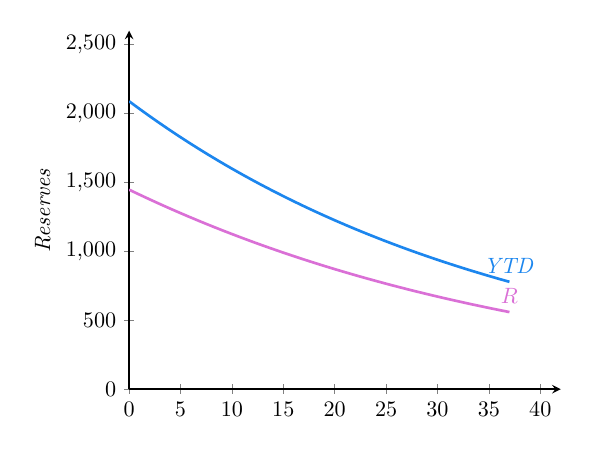
\begin{tikzpicture}[scale=0.8]
		\begin{axis}[axis x line=bottom, axis y line=left,
		xtick={0,5,...,40}, ytick={0,500,...,2500}, xmax=42, ymin=0, ymax=2600, ylabel=$\mathit{Reserves}$,
		y tick label style={/pgf/number format/.cd,fixed,fixed zerofill,precision=0,/tikz/.cd}]
		\addplot[Orchid,very thick,mark=none,domain=0:37,samples=200]
		{1446*(1-0.0625)^(\x) + 0.0263*2087*(((1-0.0625)^(\x)-(1-0.0263)^(\x))/(0.0263-0.0625))} node[above] {$R$};
		\addplot[DodgerBlue2,very thick,mark=none,domain=0:37,samples=200]
		{2087*(1-0.0263)^(\x)} node[above] {$\mathit{YTD}$};
		\end{axis}
		\end{tikzpicture}
	} \qquad
	\subfloat[][\scriptsize{$\rho$=6\%, $\xi$=8.61\%, $R_0$=1172, $\mathit{YTD}_0$=4184}]{
		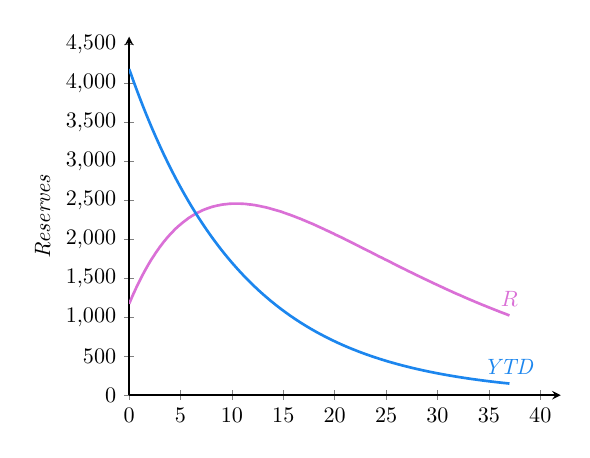
\begin{tikzpicture}[scale=0.8]
		\begin{axis}[axis x line=bottom, axis y line=left,
		xtick={0,5,...,40}, ytick={0,500,...,4500}, xmax=42, ymin=0, ymax=4600, ylabel=$\mathit{Reserves}$,
		y tick label style={/pgf/number format/.cd,fixed,fixed zerofill,precision=0,/tikz/.cd}]
		\addplot[Orchid,very thick,mark=none,domain=0:37,samples=200]
		{1172*(1-0.06)^(\x) + 0.0861*4184*(((1-0.06)^(\x)-(1-0.0861)^(\x))/(0.0861-0.06))} node[above] {$R$};
		\addplot[DodgerBlue2,very thick,mark=none,domain=0:37,samples=200]
		{4184*(1-0.0861)^(\x)} node[above] {$\mathit{YTD}$};
		\end{axis}
		\end{tikzpicture}
	} \\
	\caption{Resource profiles}
	\label{fig:deplProf}
\end{figure}

Following the assumptions from the GREEN model\footnote{\cite{Burniauxetal1992} and \cite{GREENDvdM1994}.}
\textsc{Envisage} assumes that the rate of extraction for oil and gas is
exogenous, i.e. invariant to market conditions, but that
the discovery rate is affected by market conditions.
The discovery rate will be a function of the deviation of
the market price from a given pre-determined price trend,
where the market price is the output price for individual supplies. The elasticity is allowed to differ depending on
market conditions. This kink in the discovery rate elasticity
is implemented using the sigmoid function. In addition,
we allow suppliers to be off their potential supply
curve, i.e. they can supply less than their maximum given
the exogenous extraction rate.

The key price relation that determines the elasticity
of discovery is given by equation~(\ref{eq:pRatio}).
The exogenous trend, $\mathit{PTrend}$, is indexed at 1 in the
reference year. If output prices track the trend
exactly, the $\mathit{PRatio}$ variable will always have the value of 1.
If production prices exceed the exogenous trend, the
price ratio will be above 1, i.e. market conditions
are buoyant, and vice versa if the ratio falls below 1.
Equation~(\ref{eq:omegar}) defines the elasticity according
to the price regime. As the variable $\mathit{PRatio}$ rises,
the denominator tends towards 1 and at the limit, the
active elasticity is the high elasticity. The limit of
the denominator as prices decline is $1+e^\kappa$, which for
suitably large $\kappa$ implies that the ratio  is zero and the
active elasticity is the low elasticity.

The conversion rate, $\xi$, responds to the price signal, $\mathit{PRatio}$,
where the elasticity can differ depending on market conditions. The
curve is anchored to the reference conversion rate, $\xi^{\mathit{Ref}}$.
The shifter, $\chi^d_{r,a,t}$, can be used to calibrate the
conversion rate, to an exogenous price scenario for example.
Note that the conversion rate is bounded on both ends with user
supplied lower and upper bounds. Figure~\ref{fig:convRate}
provides an illustration of the elasticity and conversion rate
curves. Note that the elasticity curve is almost virtually kinked
at the price reference point, i.e. where $\mathit{PRatio}$ is equal to 1.
On either side, the elasticity quickly moves to either the 'low' elasticity (0.3
in the figure), or the 'high' elasticity (1.2 in the figure).
The conversion rate curve has three inflection points. With very low prices the
conversion rate is bound below at 4\% and at very high prices it is bound
above at 10\%. The third inflection point is where $\mathit{PRatio}$
equals 1. The figure clearly shows the difference in the elasticity around
this inflection point, with a steeper curve when prices are increasing.

\begin{equation}
\label{eq:pRatio}
\mathit{PRatio}_{r,a,t} = \left[ \frac{\mathit{PX}_{r,a,t}/\mathit{PGDP}_{r,t}} {\mathit{PX}_{r,a,t-1}/\mathit{PGDP}_{r,t-1}} \right] \bigg / \mathit{PTrend}_{r,a,t}
\end{equation}

\begin{equation}
\label{eq:omegar}
\omega^r_{r,a,t} = \omega^{\mathit{rLo}}_{r,a,t}
+ \left(\omega^{\mathit{rHi}}_{r,a,t} - \omega^{\mathit{rLo}}_{r,a,t}\right)
/ \left[1 + \exp\left(-\kappa(\mathit{PRatio}_{r,a,t}-1) \right)\right]
\end{equation}

\begin{equation}
\label{eq:convRate}
\xi_{r,a,t} = \chi^d_{r,a,t} \xi^{\mathit{Ref}}_{r,a} \left( \mathit{PRatio}_{r,a,t} \right) ^{\omega^r_t }
\end{equation}


\begin{figure}[ht]
	\centering
	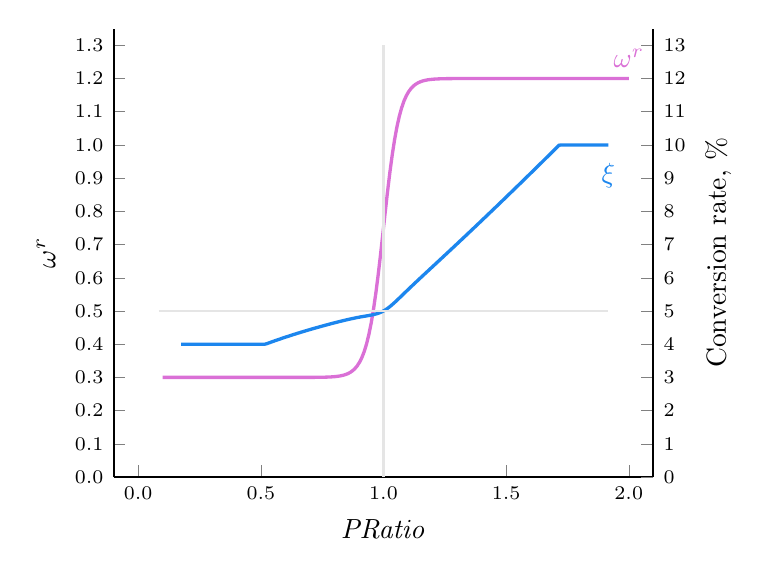
\begin{tikzpicture}

%  \pgfplotsset{
%      scale only axis,
%  }

  \begin{axis}[
    axis y line*=left,
    xlabel=$\mathit{PRatio}$,
    ylabel=$\omega^r$,
    xtick={0,0.5,...,2.0},
    yticklabel style = {font=\scriptsize},
    xticklabel style = {font=\scriptsize},
    x tick label style={/pgf/number format/.cd,fixed,fixed zerofill,precision=1,/tikz/.cd},
    ytick={0.0,0.1,...,1.3}, xmax=2.1, ymin=0, ymax=1.35,
    y tick label style={/pgf/number format/.cd,fixed,fixed zerofill,precision=1,/tikz/.cd}]
  ]
	\addplot[Orchid,very thick,mark=none,domain=0.1:2.0,samples=200]
	{0.3 + (1.2 - 0.3)/(1 + exp(-30*((\x)-1)))} node[above] {$\omega^r$};
		\addplot[lightgray,mark=none]
		coordinates{(1,0.0) (1,1.3)} ;

    \end{axis}

    \begin{axis}[
      axis y line*=right,
      axis x line=none,
      ylabel={Conversion rate, \%},
      yticklabel style = {font=\scriptsize},
      ytick={0,1,...,13}, ymin=0, ymax=13.5,
          y tick label style={/pgf/number format/.cd,fixed,fixed zerofill,precision=0,/tikz/.cd}],
    ]

 	\addplot[DodgerBlue2,very thick,mark=none,domain=0.1:2.0,samples=200]
 	{100*min(max(0.04,0.05*(\x)^(0.3 + (1.2 - 0.3)/(1 + exp(-30*((\x)-1))))),0.1)} node[below, yshift=-0.1cm] {$\xi$};
		\addplot[lightgray,mark=none]
		coordinates{(0,5) (2,5)} ;
  \end{axis}

\end{tikzpicture}
	\caption{Conversion rate curves}
	\label{fig:convRate}
\end{figure}

The extraction rate of coal is assumed to be price
sensitive and uses the same elasticity, $\omega^r$, to drive
the extraction rate. In the case of oil and gas, the
extraction rate is allowed to vary with a constant
elasticity functional form, though generally the
elasticity will be zero. Equation~(\ref{eq:xRate})
defines the extraction rate, $\rho^x$, for coal, oil and gas reserves.
For coal, the elasticity is potentially kinked and thus
there will be an inflection point for the extraction curve.
For oil and gas, the extraction elasticity is given by $\omega^e$.

\begin{equation}
\label{eq:xRate}
\rho^x_{r,a,t} =
\begin{cases}
\chi^x_{r,a,t} \rho^x_{r,a,t-1} \left( \mathit{PRatio}_{r,a,t} \right)^{\omega^r_{r,a,t}} & \textrm{if } a \in \{'Coal'\} \\
\chi^x_{r,a,t} \rho^x_{r,a,t-1} \left( \mathit{PRatio}_{r,a,t} \right)_{r,a,t}^{\omega^e_{r,a,t}} & \textrm{if } a \notin \{'Coal'\}
\end{cases}
\end{equation}

Equation~(\ref{eq:Res}) determines the actual reserve
level. It is equal to the previous period's reserve less
less actual extraction, $\mathit{Extr}$, plus the addition
of converted unproven reserves. Equation~(\ref{eq:ResP})
is the level of reserves that correspond to being on the
reserve profile, i.e. where the actual extraction is
equal to the extraction rate times the level of (lagged) reserves.
If market conditions warrant it, producers may wish to be
off their reserve profile and keep the resource underground. In
this case, actual production may be less than potential production.
Equation~(\ref{eq:resGap}) determines the gap between
actual reserves and reserves along the resource profile,
which is always a positive number.
Potential supply, equation~(\ref{eq:xfPot}) is equal to the normal level of
extraction from the reserve profile, plus what might
be available from the reserve gap, for regions that
are not forced to be on their depletion profile.

\begin{equation}
\label{eq:Res}
\mathit{Res}_{r,a,t} = \mathit{Res}_{r,a,t-1} - \mathit{Extr}_{r,a,t-1} + \xi_{r,a,t-1} \mathit{YTD}_{r,a,t-1}
\end{equation}

\begin{equation}
\label{eq:ResP}
\mathit{Res}^p_{r,a,t} = \left(1 - \rho^x_{r,a,t-1} \right) \mathit{Res}^p_{r,a,t-1} + \xi_{r,a,t-1} \mathit{YTD}_{r,a,t-1}
\end{equation}

\begin{equation}
\label{eq:resGap}
\mathit{ResGap}_{r,a,t} \ge \mathit{Res}_{r,a,t} - \mathit{Res}^p_{r,a,t}
\end{equation}

\begin{equation}
\label{eq:xfPot}
\mathit{XF}^{\mathit{Pot}}_{r,a,t} = \rho^x_t \mathit{Res}^p_{r,a,t} + \mathit{ResGap}_{r,a,t}
\end{equation}

Equation~(\ref{eq:YTD}) is the motion equation for yet-to-discover
reserves---simply previous unproven reserves less those converted
to proven.

\begin{equation}
\label{eq:YTD}
\mathit{YTD}_{r,a,t} = \left( 1 - \xi_{r,a,t-1} \right) \mathit{YTD}_{r,a,t-1}
\end{equation}

\subsection{Linking depletion variables to natural resource supply}

The standard supply equation for natural resources
is modified for coal, oil and gas reserves when
the depletion module is on. Instead of determining
$\mathit{XF}^s$ as in the standard specification, it
determines, $\mathit{XF}^{\mathit{Not}}$, i.e. the notional
supply of the natural resource. So we have two variables,
the notional supply that comes from the standard natural resource
supply curve, and the potential supply, $\mathit{XF}^{\mathit{Pot}}$,
which comes from the depletion module.
Equation~(\ref{eq:xfGap}) determines the gap between notional
and potential supply. The gap variable is bounded below by zero, in
other words if potential supply is greater than notional supply,
the gap variable is set to 0.
If notional supply exceeds potential supply, producers would
like to supply more, but are constrained to the potential supply and
in this case, actual supply is equal to potential supply. On the
other hand, if notional supply is below potential supply, producers
would prefer to sell less than their potential and will
supply the notional amount. The gap between the actual and
potential supply is then kept in the ground. These
conditions are captured in equation~(\ref{eq:xfsdepl}). If
the gap is zero, actual supply is equal to notional supply
and below potential. If the gap is positive, actual supply is
equal to potential supply.
The level of extraction will track the actual supply of natural
resources.

\begin{equation}
\label{eq:xfGap}
\mathit{XF}^{\mathit{Gap}}_{r,a,t} \ge \mathit{XF}^{\mathit{Not}}_{r,a,t} - \mathit{XF}^{\mathit{Pot}}_{r,a,t}
\end{equation}

\begin{equation}
\label{eq:xfsdepl}
\mathit{XF}^{\mathit{s}}_{r,a,t} = \mathit{XF}^{\mathit{Not}}_{r,a,t} - \mathit{XF}^{\mathit{Gap}}_{r,a,t}
\end{equation}

\begin{equation}
\label{eq:extr}
\mathit{Extr}_{r,a,t} = \mathit{Extr}_{r,a,t-1} \left(\frac{\mathit{XF}_{r,\mathit{nrs},a,t}}{\mathit{XF}_{\mathit{nrs},a,t-1}}\right)
\end{equation}

\section{Knowledge module}

[NEW 20-JAN-2019] The model includes a knowledge
module that operates somewhat similarly to investment
and the capital stock. Each year there is aggregate expenditure
on research and development (R\&D), that is captured
by the variable $\mathit{XFD}_{\mathit{r\_d}}$. This
expenditure flow increases knowledge, though knowledge
also depreciates each year. The main difference
with the usual capital/investment dynamic,
is that the impact
of R\&D expenditures happens with a distributed lag.\footnote{This
formulation is inspired by \cite{SmeetsKristkova2016}.}
The latter is governed by a \emph{Gamma} distribution
function, the parameters and length of which
are region specific.\footnote{Additional details
and example distribution functions are provided
in Annex~\ref{sec:knowledge}.}

Equation~(\ref{eq:kn}) describes the motion equation for knowledge.
The variable $\mathit{KN}$ represents
the stock of knowledge. It is equal to the previous
period's knowledge stock---adjusted by depreciation, $\delta^k$---,
plus the distributed lag of current
and previous expenditures on R\&D, where $\gamma^k$
represents the lag coefficients.\footnote{If
$\gamma^k_0=0$ and $\gamma^k_{1}=1$, the equation
would have the same assumption as the standard
capital accumulation equation.}
Annex~\ref{sec:knowledge} describes how the
model implements the knowledge module. Implementation
requires taking into account two features. (1) It is implemented
using the variable time step that is a central
part of the model. Because of the distributed
lags, this also requires that the R\&D expenditures
be evaluated each \emph{year}, independently of
the time step. (2) The first years of the simulation require
a backward projection of the R\&D expenditures,
i.e. prior to the initial year. If $N$ is 50
for example, it requires projecting R\&D
expenditures back some 50 years.

\begin{equation}
\label{eq:kn}
\mathit{KN}_{r,t} = \left(1-\delta^k_r \right) \mathit{KN}_{r,t-1}
+ \sum_{i=0}^N{\gamma^k_{r,i} \mathit{XFD}_{r,\mathit{r\_d},t-i}}
\end{equation}

\noindent where
\[
\gamma^k_{i} = \chi \left(i + 1 \right)^{\delta/(1-\delta)}\lambda^i
\]

In its default mode, the user inputs R\&D expenditures as
a (percent) share of reference year GDP. The default closure
fixes the (real) GDP share of R\&D expenditures at the reference
year level. The model specification assumes that R\&D expenditures
are paid for from government revenues.

The knowledge module is designed to impact on labor
productivity growth. Equation~(\ref{eq:pik}) describes the relation
between the endogenous component of labor productivity
in sector $a$, $\pi^k$, relative to the growth rate of the stock
of knowledge. The elasticity is given by $\epsilon^r$ and
is allowed to be sector specific. The shifter, $\gamma^r$, is initialized
at 1.

\begin{equation}
\label{eq:pik}
\pi^k_{r,a,t} = \gamma^r_{r,a,t} \epsilon^r_{r,a,t}
\left(\frac{\mathit{KN}_{r,t}}{\mathit{KN}_{r,t-1}} - 1\right)
\end{equation}

\section{Technology shifts}

By default, changes in technology are largely exogenous, for example autonomous
energy efficiency improvement (AEEI) and improvements in international trade and
transport services. The one exception is labor productivity.
Equation~(\ref{eq:lambdal}) describes the growth in labor productivity. In the
base year, $\lambda^f$ is initialized to 1, and is set to grow at a rate of
$\gamma^l$ each year. If $\alpha^{\mathit{gl}}$ is set to 0 and
$\beta^{\mathit{gl}}$ is set to 1, then labor productivity grows at a uniform
rate across all activities. There are multiple strategies to put values on these
parameters. These may include setting $\beta^{\mathit{gl}}$ to 0 for a subset of
activities and initializing $\alpha^{\mathit{gl}}$ to some exogenous level based
on external studies---for example setting $\alpha^{\mathit{gl}}$ to 2~percent in
the agricultural sectors. The remaining sectors could be segmented into two
subsets---one with high productivity, e.g. set $\alpha^{\mathit{gl}}$ to
2~percent, and one with low productivity, e.g. set $\alpha^{\mathit{gl}}$ to 0,
with $\beta^{\mathit{gl}}$ set to 1 in both cases.

Two other factors can influence sector-specific labor productivity. The first is
a skill-specific shifter, $\chi^{\mathit{gl}}$, that introduces biased technical change across skill
types. In typical simulations, this factor is initialized at 0 and there is
no difference in labor productivity growth across skills. One alternative
strategy is to have some (exogenous) assumption on the skill premium, for example
no change in the skill premium. It is then possible to endogenize skill-biased
technical change to see how much this parameter must change to maintain the
exogenous assumption on the skill premium. The second factor is the
knowledge-induced endogenous technical change, $\pi^k$. This formulation
is described in the knowledge module, see for example equation~(\ref{eq:pik}).

In the baseline or reference
scenario, $\gamma^l$ will be calibrated to target a given level of per capita
GDP growth and subject to the assumptions made on $\alpha^{\mathit{gl}}$ and
$\beta^{\mathit{gl}}$. In subsequent scenarios, $\lambda^f$ will be exogenous
having been calibrated in the reference scenario, subject to any changes
in the two other factors: $\chi^{\mathit{gl}}$ and $\pi^k$.

\begin{equation}
\label{eq:lambdal}
\lambda^f_{r,l,a,t} =
   \left( 1 + \chi^{\mathit{gl}}_{r,l,t} + \pi^k_{r,a,t} + \alpha^{\mathit{gl}}_{r,l,a,t}
+  \beta^{\mathit{gl}}_{r,l,a,t} \gamma^l_{r,t} \right)^n \lambda^f_{r,l,a,t-n}
\end{equation}

Because \emph{Old} capital is malleable, the cost structure of \emph{Old} capital is
adjusted between periods in such a way that the aggregate inputs of the previous period (i.e.
summed over vintages) can produce aggregate output. There is no such adjustment of the
cost structure of \emph{New} capital. In generic terms, for any nest in the production structure
we have inputs $X_{i,v,t}$ at price $P_{i,v,t}$ to form the bundle $V_{v,t}$ at price $R_{v,t}$,
with technological shifters given by $\lambda_{i,v,t}$. The basic re-calibration formula is:

\[
\alpha_{i,\mathit{Old},t+1} =
\lambda_{i,\mathit{Old},t}^{\left(1-\sigma_{\mathit{Old}}\right)}
\frac{\displaystyle \sum_v{X_{i,v,t}}} {\displaystyle \sum_v{V_{v,t}}}
\left[
\frac{\displaystyle {\sum_v{P_{i,v,t} X_{i,v,t}}} \biggl / {\sum_v{X_{i,v,t}}}} {\displaystyle {\sum_v{R_{v,t} V_{v,t}}} \biggl / {\sum_v{V_{v,t}}}}
\right]^{\sigma_{\mathit{Old}}}
\]

\noindent where $\sigma$ is the relevant substitution elasticity for \emph{Old} capital. The formula remains the same for the normalized version of the CES
function.

\section{Servitization}

[Added 13-FEB-2022] Code has been introduced to allow for
the 'servitization' of the economy, essentially defined as the change
in the production structure that rotates towards services
demand away from manufactured demand. The implementation
is based on the description from \cite{ChateauetalSupplyJGEA2020}.

Let $k$ represent the 'services' inputs, $m$ represent the
manufactured inputs, and $c$ represent the union of the two.\footnote{In
\cite{ChateauetalSupplyJGEA2020} $k$ represents all non-transport services,
(though it is unclear how 'ELY' and 'CNS' are treated.
It is also not clear what is included in the manufactured inputs, e.g. energy?).}
The basic idea is to raise the
share of services inputs each year by a growth factor, for example
1\%, and to adjust downwards the the share of manufactured
inputs. A cap is introduced on the share, for example 60\%.\footnote{In
\cite{ChateauetalSupplyJGEA2020} the 1\% and 60\% assumptions
apply to the manufacturing activities. The relevant
numbers in the services sectors are 0.2\% and 75\%.}
In \textsc{Envisage}, this is done in a cost-neutral fashion,
i.e. using the 'twist' methodology---further described in the next section
and in Appendix~\ref{chap:CESAppendix}.

The initial share of services in activity $a$
with respect to all relevant inputs, i.e. $c$, is given by the
following formula. Note that the denominator does not quite have the
same value as the $\mathit{ND1}$ bundle, as it excludes some inputs
such as transport services.

\[
s^t_{a,t0} = \displaystyle \frac{\sum_k{\mathit{PA}_{k,a,t0}\mathit{XA}_{k,a,t0}}}
{\sum_c{\mathit{PA}_{c,a,t0}\mathit{XA}_{c,a,t0}}}
\]

The following expression provides the desired growth in the share of
services in production, where $\mathit{gs}$ is the user-provided growth
rate. The share is capped at $\mathit{smax}^t$.
\[
s^t_{a,t} = min\left[s^t_{a,t-n} \left(1 + \mathit{gs}_{a} \right)^n, \mathit{smax}^t_{a,t}\right]
\]

Equations~(\ref{eq:ios}) and~(\ref{eq:iom}) represent the update formulas for
the input-output technology parameters that thus incorporate
the servitization assumption.

\begin{equation}
\label{eq:ios}
\lambda^{\mathit{io}}_{k,a,t} = \lambda^{\mathit{io}}_{k,a,t-1}
\left(\frac{s^t_{a,t-1}}{s^t_{a,t}}
\right)^{1/(1-\sigma^{\mathit{nd1}}_{a})}
\end{equation}

\begin{equation}
\label{eq:iom}
\lambda^{\mathit{io}}_{m,a,t} = \lambda^{\mathit{io}}_{m,a,t-1}
\left(\frac{1 - s^t_{a,t-1}}{1 - s^t_{a,t}}
\right)^{1/(1-\sigma^{\mathit{nd1}}_{a})}
\end{equation}

It is pretty straightforward to show that the so-called 'twist' variable
takes the following form in this case:

\[
\mathit{tw}_{a,t} = \frac{s^t_{a,t} - s^t_{a,t-1}}{s^t_{a,t-1}\left(1 - s^t_{a,t}\right)}
\]

\section{Preference shifters}

\subsection{Armington twists}

In the standard version of the model, the Armington preference parameters---both
top and second levels---are held fixed at their base year calibrated levels.
Thus changes in import shares are linked only to changes in relative prices.
Historically, we have observed large changes in import shares without a
concomitant change in relative prices. \cite{DixonRimmer2002} have developed a
specification for the MONASH (and USAGE) model that 'twists' the relevant share
parameters. The 'twist' targets a percentage change in the ratio of imports to
domestic demand, which at unchanged component prices, is cost-neutral. The
mechanics of the twist methodology is described in
Appendix \ref{chap:CESAppendix}.

For the \textsc{Envisage} model, we have incorporated three versions of the
twist---for the dual nested sourcing decision. The first two deal with the
top-level Armington decision---purchases of domestic goods and the aggregate
import bundle. Since we have two possible specifications---agent-based sourcing
or national sourcing, we provide two twist specifications. The third is for the
second level nest that sources aggregate imports by region of origin.

\subsubsection{National sourcing}

The equations for national sourcing of domestic purchases and aggregate imports
are provided in equations~(\ref{eq:xdt}) and~(\ref{eq:xmt}), with the domestic
and import share parameters given respectively by $\alpha^{\mathit{dt}}$ and
$\alpha^{\mathit{mt}}$. Equation~(\ref{eq:twt1}) provides the 'twisted' domestic
and imported share parameters where $\mathit{tw}^{\mathit{t1}}$ is the level of
the desired twist, i.e. the percent change in the ratio of imports to domestic
purchases at unchanged prices. The twist has no impact on the share parameters
if it is set to its default value of 0. The twist updating uses the (lagged)
value share of imports in the top-level Armington bundle.\footnote{In the MONASH
and USAGE models, the twist parameters are calculated contemporaneously, i.e.
they are part of the model equations. In \textsc{Envisage}, the twists are
applied between periods. This should have only minimal impact on model results.}
Note that the formulas apply the twist factor directly to the share coefficients
themselves and we drop the $\lambda$ factor, i.e. preference change variable,
from the formulas as these can be substituted out (refer to
Appendix \ref{chap:CESAppendix}).

\begin{equation}
\label{eq:twt1}
\begin{array}{c c l}
   \alpha^{\mathit{dt}}_{r,i,t} & = &
      \alpha^{\mathit{dt}}_{r,i,t-1}
      \frac {\displaystyle 1} {\displaystyle 1+s^{\mathit{t1}}_{r,i,t-1}
         \mathit{tw}^{\mathit{t1}}_{r,i,t}} \\
   \alpha^{\mathit{mt}}_{r,i,t} & = &
      \alpha^{\mathit{mt}}_{r,i,t-1}
      \frac{\displaystyle 1+\mathit{tw}^{\mathit{t1}}_{r,i,t}}
         {\displaystyle 1+s^{\mathit{t1}}_{r,i,t-1}
            \mathit{tw}^{\mathit{t1}}_{r,i,t}} \\
\end{array}
\end{equation}

\noindent where

\[
s^{\mathit{t1}}_{r,i,t-1} = \frac{\mathit{PMT}_{r,i,t-1}\mathit{XMT}_{r,i,t-1}}
   {\mathit{PAT}_{r,i,t-1}\mathit{XAT}_{r,i,t-1}}
\]

\subsubsection{Agent sourcing}

The expressions for agent-based sourcing of domestic goods and aggregate imports
are nearly identical with the inclusion of the index for the Armington agent,
$\mathit{aa}$. The share parameters are part of equations~(\ref{eq:xd})
and~(\ref{eq:xm}). Equation~(\ref{eq:tw1}) provides the relevant formulas for
the 'twisted' shares using the appropriate import share level. Note that the
twists are allowed to be agent-specific, though in practice, there is probably
little evidence to differentiate across agents.

\begin{equation}
\label{eq:tw1}
\begin{array}{c c l}
\alpha^{\mathit{d}}_{r,i,\mathit{aa},t} & = &
   \alpha^{\mathit{d}}_{r,i,\mathit{aa},t-1}
   \frac{\displaystyle 1}{\displaystyle 1+s^{\mathit{1}}_{r,i,\mathit{aa},t-1}
      \mathit{tw}^{\mathit{1}}_{r,i,\mathit{aa},t}} \\
\alpha^{\mathit{m}}_{r,i,\mathit{aa},t} & = &
   \alpha^{\mathit{m}}_{r,i,\mathit{aa},t-1}
   \frac{\displaystyle 1+\mathit{tw}^{\mathit{1}}_{r,i,\mathit{aa},t}}
   {\displaystyle 1+s^{\mathit{1}}_{r,i,\mathit{aa},t-1}
      \mathit{tw}^{\mathit{1}}_{r,i,\mathit{aa},t}} \\
\end{array}
\end{equation}

\noindent where

\[
s^{\mathit{1}}_{r,i,\mathit{aa},t-1} =
   \frac{\mathit{PM}_{r,i,\mathit{aa},t-1}\mathit{XM}_{r,i,\mathit{aa},t-1}}
   {\mathit{PA}_{r,i,\mathit{aa},t-1}\mathit{XA}_{r,i,\mathit{aa},t-1}}
\]

\subsubsection{Second level Armington twists}

The second level of the Armington nest allocates aggregate imports across source
regions (see equation~(\ref{eq:xwd})). With the sole exception of a 2-region
model, the standard twist does not apply and we thus apply the twist to a target
set of source countries, i.e. we segment the source regions
into~2.\footnote{The targeted regions can include only a single region.} The
targeted regions will see their share increase (by the same twist), and the
non-targeted regions will see their share decline.

\begin{equation}
\label{eq:tw2}
\begin{array}{c c l l}
\alpha^{\mathit{w}}_{s,i,r,t} & = &
   \alpha^{\mathit{w}}_{s,i,r,t-1}
   \frac{\displaystyle 1}{\displaystyle 1+s^{\mathit{2}}_{i,r,t-1}
      \mathit{tw}^{\mathit{2}}_{r,i,t}}
&  \textrm{if } s \notin {\mathit{rtwtgt}(s,r)}\\
\alpha^{\mathit{w}}_{s,i,r,t} & = &
   \alpha^{\mathit{w}}_{s,i,r,t-1}
   \frac{\displaystyle 1+\mathit{tw}^{\mathit{2}}_{r,i,t}}
      {\displaystyle 1+s^{\mathit{2}}_{i,r,t-1} \mathit{tw}^{\mathit{2}}_{r,i,t}}
&  \textrm{if } s \in {\mathit{rtwtgt}(s,r)} \\
\end{array}
\end{equation}

\noindent where
\[
s^{\mathit{2}}_{i,r,t-1} =
   \frac{\sum_{s \in {\mathit{rtwtgt}(s,r)}}
      {\mathit{PDM}_{s,i,r,t-1}\mathit{XW}_{s,i,r,t-1}}}
      {\sum_{s}{\mathit{PDM}_{s,i,r,t-1}\mathit{XW}_{s,i,r,t-1}}}
\]

\subsection{Introducing cost curves}

Changes in costs in the normal functioning of the model depend on changes in
input prices and the standard assumptions regarding technology change. This
section explains how to introduce an acceleration in cost reduction coming from
some exogenous phenomenon such as learning by doing. The basic idea is to start
from an initial price, say $P_0$, and to reduce costs over time, albeit with a
lower limit given by $\mathit{PMIN}$. There also exists a target price for year
$T$, given by $P_T$, that must be greater than $\mathit{PMIN}$. Let $\alpha$
represent the ratio of the final price, $P_T$, relative to the base year price,
$P_0$, i.e.:

\[
P_T=\alpha P_0
\]

\noindent and let $\gamma$ represent the ratio of the minimum price,
$\mathit{PMIN}$, relative to the initial price, i.e.:

\[
\mathit{PMIN}=\gamma P_0
\]

\noindent where $\alpha > \gamma$. Two functional forms are introduced to
represent the cost curve---the hyperbola and the logistic functions. The
hyperbola takes the following form:

\[
P_t = \mathit{PMIN} + \chi t^{-\beta}
\]

\noindent The logistic function takes the form:

\[
P_t = \frac{\mathit{PMIN}} {1+\chi e^{-\beta t}}
\]

Calibration of the parameters for the hyperbola function involve the following
expressions:

\[
\begin{array}{c c}
\beta = \displaystyle \frac{\ln\left(\displaystyle
   \frac{\alpha-\gamma}{1-\gamma}\right)}
      {\ln\left(\displaystyle \frac{t_0}{T}\right)}
&  \qquad \chi = P_0\left(1-\gamma\right) \\
\end{array}
\]

\noindent where we define $t_0$ to start with 1.\footnote{If the first year is
2011, $t$ is then defined as $t-2010$. If 	the final year is 2050, then $T$ is
equal to $2050 - (2011-1)=40$.} In the case of the logistic function, the
calibration formulas are:

\[
\begin{array}{c c}
\beta = \displaystyle - \frac{1}{T} \ln \left( \displaystyle
   \frac{\alpha-\gamma}{\alpha\left(1-\gamma\right)}\right)
&  \qquad \chi = \gamma-1 \\
\end{array}
\]

\noindent where we define $t_0$ to start with 0.\footnote{If the first year is
2011, $t$ is then defined as $t-2011$. If 	the final year is 2050, then $T$ is
equal to $2050 - 2011=39$.} Figure~\ref{fig:costCurve} depicts the shapes of the
two cost curves for the same initial and end points and price limit. From the
shape of the curves it is clear that costs drop sharply in the initial years
using the hyperbola specification. The drop is more gradual (and constant in
percentage terms) for the logistic function.

\begin{figure}
   \centering
   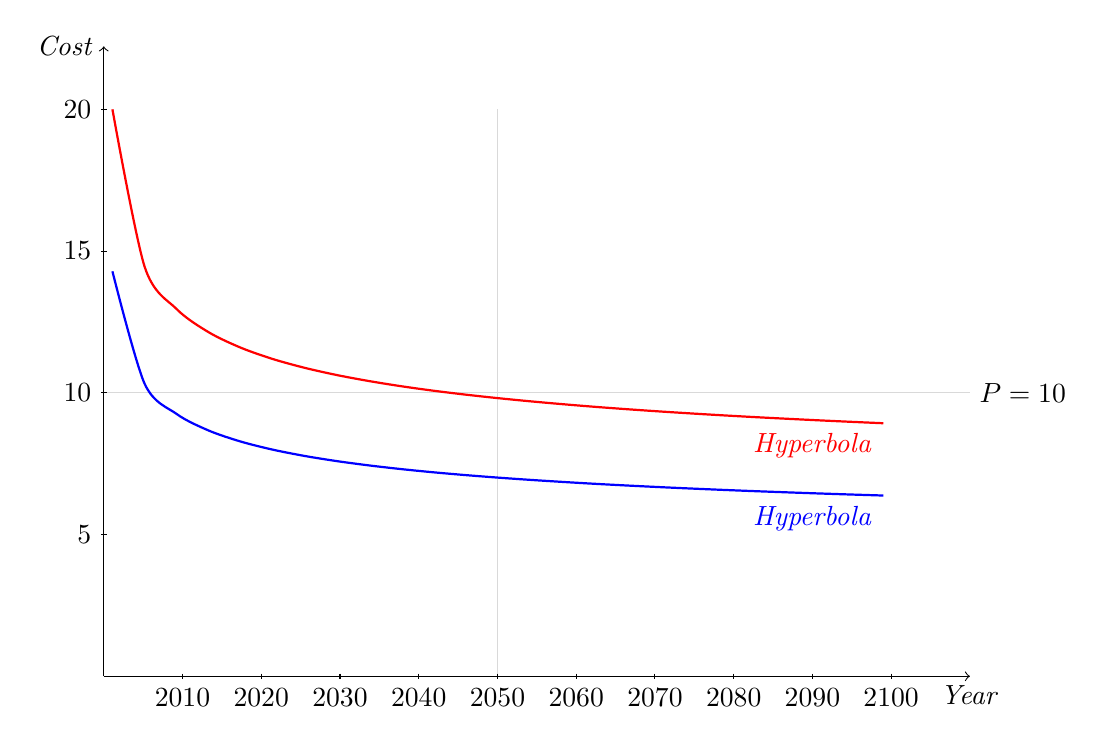
\begin{tikzpicture}
%\begin{tikzpicture}[x=1.2cm,y=0.4cm]

%\draw[help lines] (0,0) grid (13,13);

%  Draw the axes
\draw[->] (0,0) -- (11,0) node[below] {\emph{Year}};
\draw[->] (0,0) -- (0,8.0) node[left] {\emph{Cost}};

\draw[color=gray!30] (0,2*1.8) -- (11,2*1.8) node[right] {\color{black}{$P=10$}};
\draw[color=gray!30] (5,0) -- (5,4*1.8) node[below right] {};
%\draw[color=gray!30] (0,2) -- (2.5,2) node[below right] {\color{black}{$\eta=2.0$}} ;

\foreach \x in {1,...,10}
	\draw (\x cm, 1pt) -- (\x cm, -1pt) node[anchor = north]
	{\pgfmathparse{int(2000+10*\x)}${\pgfmathresult}$};

\foreach \y in {1,...,4}
	\draw (1pt, \y*1.8 cm) -- (-1pt, \y*1.8 cm) node[anchor = east]
	{\pgfmathparse{int(0+5*\y)}${\pgfmathresult}$};

\draw[scale=1,domain=0.11:9.9,smooth,variable=\x,red,thick] plot 
({\x},{(5+(20*(1-5/20))*((2110-2010)/11*\x)^(-ln((5/10-5/20)/(1-5/20))/ln(1/(2050-(2011-1)))))/(5/1.8)}) node[below left] {\emph{Hyperbola}};
\draw[scale=1,domain=0.11:9.9,smooth,variable=\x,blue,thick] plot 
({\x},{(5+(20*(1-5/20))*((2110-2010)/11*\x)^(-ln((5/10-5/20)/(1-5/20))/ln(1/(2050-(2011-1)))))/(7/1.8)}) node[below left] {\emph{Hyperbola}};
\end{tikzpicture}

   \caption{Examples of cost curves}
   \label{fig:costCurve}
\end{figure}

The adjustment to the cost curve is made on total factor productivity (TFP) for
the relevant activity. The aggregate cost is given by the following formula:

\[
P_t = \frac{1}{\lambda_t} F(P_{i,t})
\]

\noindent where $F$ is the cost function and depends on the prices of the
various inputs given by $P_i$. In most cases, the cost function will be the dual
price expression of the CES function.\footnote{In 	most cases $\lambda$ is
initialized at 1 and is held constant. Technology is introduced as
labor-augmenting technical change and with an exogenous improvement in
energy efficiency.} TFP is assumed to behave according to the following
expression:

\[
\lambda_t = \left(1+\pi_t\right)^n \lambda_{t-n}
\]

Assuming that input prices are invariant, the growth in TFP must be equal to the
following expression:

\[
\pi_t = \left( \frac{P_{t-n}}{P_t} \right)^{1/n} -1
\]

We can introduce the formulas for the two cost curves to derive expressions for
$\pi$. For the hyperbola, we have:

\[
\pi_t =
   \left( \frac{\mathit{PMIN}+\chi(t-n)^{-\beta}}
      {\mathit{PMIN}+\chi t^{-\beta}} \right)^{1/n} -1
\Longleftrightarrow
   \left( \frac{\gamma + (1-\gamma)(t-n)^{-\beta}}
      {\gamma + (1-\gamma) t^{-\beta}} \right)^{1/n} -1
\]

\noindent For the logistic function, the expression for $\pi$ is given by:

\[
\pi_t =
   \left( \frac{e^{\beta t} + \chi}{e^{\beta t} + \chi e^{\beta n}}
   \right)^{1/n} -1
\]

Both changes in preferences and introduction of the cost curves can be
implemented to change the share of any technology in a demand bundle. The latter
operates directly on the preference shares of the buyer. The former operates on
the perceived cost of the technology. These are formulated independently of the
actual cost changes that arise from the endogenous changes in input prices.

\subsubsection{Alternative cost curves}

One alternative for the hyperbolic cost curve is to calibrate the curve through
three data points: the reference year and two future years---respectively $t_0$,
$t_1$ and $t_2$. The curve can be defined by:

\[
P_t = P_{t_0} + \chi \left(t-t_0\right)^{-\beta}
\]

\noindent The exponent can be calibrated using the following formula:

\[
\beta = \ln \left( \frac{P_{t_1}-P_{t_0}}{P_{t_2}-P_{t_0}} \right) /
\ln \left( \frac{t_2 - t_0}{t_1 -  t_0} \right)
\]

\noindent The slope coefficient can be calibrated using:

\[
\chi = \left(P_{t_1} - P_{t_0}\right) \left(t_1-t_0\right)^{\beta}
\]

\subsection{Electrification preferences}

Each agent in the economy has demand for an aggregate
energy bundle. The parameters are calibrated to the
base year data---and in many instances, most agents
have relatively low shares for electricity demand. It might
thus prove desirable to autonomously increase electrification
to a user's targeted share. The formulas below
are introduced assuming constant prices and ignoring
the re-calibration of \emph{'Old'} share parameters
that is part of a dynamic simulation. The relevant
preference parameters are equal to the ratio
of the target share in year $t$ relative to the
actual base year share. The target share can be some
multiple of the base year share, or any other assumption
desired by the user. Note that it is up to the user to
make sure that the targeted share is within a normal
range.

Calibrated preference parameters between electric and
non-electric bundles in production.

\[
\alpha^{\mathit{ely}}_{\mathit{r,a,v,t}}
= \frac{s^{\mathit{ely}}_{r,a,t}}{s^{\mathit{ely}}_{r,a,t_0}}
\]

\[
\alpha^{\mathit{nely}}_{\mathit{r,a,v}}
= \frac{1-s^{\mathit{ely}}_{r,a,t}}{1-s^{\mathit{ely}}_{r,a,t_0}}
\]

\noindent Calibrated preference parameters between electric and
non-electric bundles in consumption.

\[
 \alpha^{\mathit{cely}}_{\mathit{r,k,h,t}}
= \frac{s^{\mathit{cely}}_{r,h,t}}{s^{\mathit{cely}}_{r,h,t_0}}
\]

\[
\alpha^{\mathit{cnely}}_{\mathit{r,k,h,t}}
= \frac{1-s^{\mathit{cely}}_{r,k,h,t}}{1-s^{\mathit{cely}}_{r,k,h,t_0}}
\]

If the user provides a target share for some future year, say $T$\footnote{$T$ is often the final year of a simulation.}, the intermediate shares can be adjusted using several different
smoothing assumptions, for example geometric or arithmetic growth.

\[
s^{\mathit{ely}}_{r,a,t} =
\begin{cases}
s^{\mathit{ely}}_{r,a,t_0}
\left[\frac{s^{\mathit{ely}}_{r,a,T}}{s^{\mathit{ely}}_{r,a,t_0}}
\right]^{(t-t_0)/(T-t_0)} & \textrm{if } t < T \textrm{ and geometric growth} \\
s^{\mathit{ely}}_{r,a,t_0} +
\left[{s^{\mathit{ely}}_{r,a,T}}-{s^{\mathit{ely}}_{r,a,t_0}}
\right]
\displaystyle \frac{t-t_0}{T-t_0} & \textrm{if } t < T \textrm{ and arithetic growth} \\
s^{\mathit{ely}}_{r,a,T} & \textrm{if } t \ge T
\end{cases}
\]

\section{Implementation}

The \texttt{core} model includes all of the equations from
Chapter~3.\footnote{With the exception of the GDP per capita growth equation as
this requires a different MCP formulation.} There are two versions of the
dynamic model. The reference simulation, that targets GDP growth, is defined as
the \texttt{core} model plus the GDP growth equation (\ref{eq:grgdppc}),
migration (\ref{eq:migr}), labor supply by skill and zone (\ref{eq:ls}), total
labor supply by skill (\ref{eq:glab}), investment growth factor
(\ref{eq:invgfact}), non-normalized capital stock (\ref{eq:kst}), normalized
capital stock (\ref{eq:tks}), and labor productivity (\ref{eq:lambdal}). This
model is called \texttt{coreBaU} and it essentially calibrates the economy-wide
labor productivity factor. All other dynamic simulations assume that labor
productivity is exogenous i.e. per capita GDP growth is endogenous. This model
is called \texttt{coreDyn} and includes the \texttt{core} model plus the GDP
growth equation (\ref{eq:grgdppc}), migration (\ref{eq:migr}), labor supply by
skill and zone (\ref{eq:ls}), total labor supply by skill (\ref{eq:glab}),
investment growth factor (\ref{eq:invgfact}), non-normalized capital stock
(\ref{eq:kst}), and normalized capital stock (\ref{eq:tks}).

\section{Diagnostics}

There are a number of post-simulation diagnostics available with the model. Most
are relatively straightforward and need no additional explanation, for example
the GDP deflator at market price---these are taken directly from the model
solution file and aggregated where appropriate.

\subsection{Sectoral investment}

Sectoral investment can be backed out by the capital accumulation motion
equation:

\[
I_{a,t} = K_{a,t+1} - (1-\delta)K_{a,t}
\]

\section{Exogenous variables}

In this section, we summarize the standard list of
exogenous variables in the model. These are partitioned
into sub-groups depending on their role in the model
specification.

\subsection{Factors of production}

Population and labor force growth are typically exogenous. The latter
may be defined over rural and urban if using the migration module. In
this case, the growth of labor is exogenous, but the growth per zone
may be influenced by endogenous rural to urban migration. The capital
stock is exogenous in the comparative static version of the model
and is in principle pre-determined in the dynamic model with annual
step sizes. In the case of multi-year step size, current investment
will influence the current stock level (see equation~(\ref{eq:kst})).
Natural resources are supplied with an upward sloping supply curve
with two, normally fixed, shifters. The first shifter is a regional
shifter. The second is a global shifter. The latter has been used to
target a trend for world prices (e.g. oil or gas). In this case
the world price for the relevant sector is fixed to the desired
trend level and the global resource supply shifter is endogenous. This
would typically be implemented only in a baseline. The land
and water asymptotes are used-entered, as is the demand for
exogenous water bundles.

\begin{table}[H]
	\caption{Exogenous factor variables}
	\label{tab:exogFact}
	\begin{center}
		\rowcolors{2}{TableOdd}{TableEven}
		\rowcolors{1}{}{lightblue}
		\begin{tabular}{l l p{8.0cm}}
			\arrayrulecolor{TableBorder}\specialrule{1pt}{0pt}{0pt}
			\textbf{Variable} & \textbf{GAMS} & \textbf{Description} \\
			\arrayrulecolor{TableBorder}\specialrule{1pt}{0pt}{0pt}
{$\mathit{Pop}^t$} & {\texttt{pop}} & {Population} \\
{$g^{\mathit{lz}}$} & {\texttt{glabz}} & {Growth of labor by zone} \\
{$\chi^{rw}$} & {\texttt{chirw}} & {Reservation wage shifter} \\
{$K^s$} & {\texttt{kstock}} & {Capital stock (endogenous in dynamic version)} \\
{$\mathit{TK}^s$} & {\texttt{tkaps}} & {Normalized capital stock (endogenous in dynamic version)} \\
{$\chi^{w,\mathit{nrs}}$} & {\texttt{wchinrs}} & {Global natural resource supply shifter} \\
{$\chi^{\mathit{nrs}}$} & {\texttt{chinrs}} & {Region specific natural resource supply shifter} \\
{$\mathit{PW}$} & {\texttt{pw}} & {World price by activity} \\
{$\mathit{TLand}^{\mathit{Max}}$} & {\texttt{landmax}} & {Land maximum} \\
{$\mathit{TH2O}^{\mathit{Max}}$} & {\texttt{h2oMax}} & {Water maximum} \\
{$\mathit{H2OBnd}_{\mathit{wbx}}$} & {\texttt{h2obnd}} & {Exogenous water bundle demand} \\
			\arrayrulecolor{TableBorder}\specialrule{1pt}{0pt}{0pt}
		\end{tabular}
	\end{center}
\end{table}

\subsection{Macro closure}

There are three different closure rules---all with default
assumptions. The savings-investment closure fixes the household
savings rate, $\mathit{aps}$, adjusted by the shift parameter $\chi^s$.
The former is always fixed. The latter can be endogenous to achieve
a given target---for example the investment to GDP ratio. The latter
is endogenous under the default closure rule but may be over-ridden.
Typically, in the baseline, one will target some level of
the investment to GDP ratio and allow the private savings rate adjust.\footnote{The targeted investment variable is \texttt{rinvshr} in the
GAMS code.} In a similar vein, the wage premium, normally the skilled
wage relative to unskilled wages, is endogenous. One could target
the wage premium, i.e. make it exogenous. The endogenous variable
could be the relative growth of skilled and unskilled labor in levels
or the relative growth in labor productivity. The default public
closure is that government expenditures are fixed relative to GDP
in real terms (in the baseline) and real government savings are
fixed. The direct tax rate, $\kappa^h$, on household income, is
the swing variable that ensures the fiscal target. The default balance
of payment closure fixes net foreign saving. The real exchange rate
is endogenous. Two additional closures are available. One fixes
the share of foreign savings relative to GDP---similar in
many ways to the default closure. The third allows for some
endogeneity in foreign savings, in which case the deviation
of expected capital returns is equalized across all regions.

\begin{table}[H]
	\caption{Exogenous macro closure variables}
	\label{tab:exogClosure}
	\begin{center}
		\rowcolors{2}{TableOdd}{TableEven}
		\rowcolors{1}{}{lightblue}
		\begin{tabular}{l l p{8.0cm}}
			\arrayrulecolor{TableBorder}\specialrule{1pt}{0pt}{0pt}
			\textbf{Variable} & \textbf{GAMS} & \textbf{Description} \\
			\arrayrulecolor{TableBorder}\specialrule{1pt}{0pt}{0pt}
{$\mathit{aps}$} & {\texttt{aps}} & {Average savings propensity (not for ELES)} \\
{$\chi^s$} & {\texttt{chiaps}} & {Private savings shifter (depends on investment/savings closure)} \\
{$\pi^s$} & {\texttt{wprem}} & {Wage premium} \\
{$\mathit{RS}^g$} & {\texttt{rsg}} & {Real public savings (depends on fiscal closure)} \\
{$\mathit{YFD}_{\mathit{gov}}$} & {\texttt{xfd(gov)}} & {Government expenditures} \\
{$S^f$} & {\texttt{savf}} & {Foreign saving (depends on BoP closure)} \\
{$\chi^{\mathit{sf}}$} & {\texttt{savRat}} & {Foreign saving as share of GDP (depends on BoP closure)} \\
{$\mathit{PNUM}$} & {\texttt{pnum}} & {Model numeraire} \\
			\arrayrulecolor{TableBorder}\specialrule{1pt}{0pt}{0pt}
		\end{tabular}
	\end{center}
\end{table}

\subsection{Tax rates}

In the default specification all tax rates are exogenous. The actual
tax rate used could depend on model specification choices, for
example, a national versus agent-based representation of
the second level Armington specification.

\begin{table}[H]
	\caption{Exogenous tax rate}
	\label{tab:exogTax}
	\begin{center}
		\rowcolors{2}{TableOdd}{TableEven}
		\rowcolors{1}{}{lightblue}
		\begin{tabular}{l l p{8.0cm}}
			\arrayrulecolor{TableBorder}\specialrule{1pt}{0pt}{0pt}
			\textbf{Variable} & \textbf{GAMS} & \textbf{Description} \\
			\arrayrulecolor{TableBorder}\specialrule{1pt}{0pt}{0pt}
{$\tau^p$} & {\texttt{ptax}} & {Production tax} \\
{$\tau^{\mathit{uc}}$} & {\texttt{uctax}} & {Unit cost tax} \\
{$\tau^v$} & {\texttt{pftax}} & {Tax on factor use} \\
{$\kappa^f$} & {\texttt{kappaf}} & {Factor income tax by source activity and factor} \\
{$\tau^a$} & {\texttt{patax}} & {Tax on Armington consumption (depends on ArmFlag)} \\
{$\tau^{\mathit{ad}}$} & {\texttt{pdtax}} & {Tax on domestic sales of domestic goods (depends on ArmFlag)} \\
{$\tau^{\mathit{am}}$} & {\texttt{pmtax}} & {Tax on domestic sales of imported goods (depends on ArmFlag)} \\
{$\tau^e$} & {\texttt{etax}} & {Bilateral export tax} \\
{$\tau^m_{s,i,r} $} & {\texttt{mtax}} & {Bilateral import tariff} \\
{$\tau^\mathit{ma}$} & {\texttt{mtaxa}} & {Import tariff for MRIO version of model} \\
			\arrayrulecolor{TableBorder}\specialrule{1pt}{0pt}{0pt}
		\end{tabular}
	\end{center}
\end{table}

\subsection{Technology variables}

In most cases all of the technology variables are exogenous, though
not necessarily fixed at base year levels---for example, the
international trade margins or energy efficiency. The model
calibrates labor-biased technological change (the $\lambda^f$ parameter
for labor) in the baseline to target GDP growth. In this case, $g^y$, i.e.
per capita output growth, is exogenous, and $\gamma^l$ is endogenous.
An equation in the model evaluates $\lambda^f$ for labor based
on the exogenous GDP growth target. In all subsequent simulations the
labor productivity variable is fixed and GDP growth is endogenous.

\begin{table}[H]
	\caption{Exogenous technology variables}
	\label{tab:exogTech}
	\begin{center}
		\rowcolors{2}{TableOdd}{TableEven}
		\rowcolors{1}{}{lightblue}
		\begin{tabular}{l l p{8.0cm}}
			\arrayrulecolor{TableBorder}\specialrule{1pt}{0pt}{0pt}
			\textbf{Variable} & \textbf{GAMS} & \textbf{Description} \\
			\arrayrulecolor{TableBorder}\specialrule{1pt}{0pt}{0pt}
{$\zeta^{\mathit{mg}}$} & {\texttt{tmarg}} & {Bilateral trade margins} \\
{$A^{\mathit{xpv}}$} & {\texttt{axghg}} & {Uniform shifter in production bundle} \\
{$\lambda^{\mathit{xp}}$} & {\texttt{lambdaxp}} & {Output shifter in production bundle} \\
{$\lambda^{\mathit{ghg}}$} & {\texttt{lambdaghg}} & {GHG shifter in production bundle} \\
{$\lambda^f$} & {\texttt{lambdaf}} & {Productivity parameter for primary factors} \\
{$\lambda^k$} & {\texttt{lambdak}} & {Capital efficiency shifter} \\
{$\lambda^{h2ob}$} & {\texttt{lambdah2obnd}} & {Water efficiency shifter in water bundle use} \\
{$\lambda^{\mathit{io}}$} & {\texttt{lambdaio}} & {Efficiency shifter in intermediate demand} \\
{$\lambda^{\mathit{e}}$} & {\texttt{lambdae}} & {lambdae} \\
{$\lambda^{\mathit{ce}}$} & {\texttt{lambdace}} & {lambdace} \\
{$g^y$} & {\texttt{grrgdppc}} & {Growth rate of real per capita GDP} \\
{$\gamma^l$} & {\texttt{gl}} & {Economywide labor productivity parameter} \\
\arrayrulecolor{TableBorder}\specialrule{1pt}{0pt}{0pt}
		\end{tabular}
	\end{center}
\end{table}

\subsection{Preference variables}

Preference variables are all fixed, but may depend on which
utility function is implemented. They could also be adjusted
between solution periods to target some trend growth, for
example the food budget, as incomes change.

\begin{table}[H]
	\caption{Exogenous preferences variables}
	\label{tab:exogPref}
	\begin{center}
		\rowcolors{2}{TableOdd}{TableEven}
		\rowcolors{1}{}{lightblue}
		\begin{tabular}{l l p{8.0cm}}
			\arrayrulecolor{TableBorder}\specialrule{1pt}{0pt}{0pt}
			\textbf{Variable} & \textbf{GAMS} & \textbf{Description} \\
			\arrayrulecolor{TableBorder}\specialrule{1pt}{0pt}{0pt}
{$e^h$} & {\texttt{eh}} & {CDE expansion parameter} \\
{$b^h$} & {\texttt{bh}} & {CDE substitution parameter} \\
{$\alpha^h$} & {\texttt{alphah}} & {CDE shift parameter} \\
{$\gamma$} & {\texttt{gamma}} & {AIDADS/E/LES marginal propensity to consume parameter} \\
{$\mu^c$} & {\texttt{muc}} & {AIDADS/E/LES Subsistence minima} \\
			\arrayrulecolor{TableBorder}\specialrule{1pt}{0pt}{0pt}
		\end{tabular}
	\end{center}
\end{table}

\subsection{Emission variables}

The default specification for emissions is that they are endogenous
and the emissions tax is exogenous (and in most cases set to zero\footnote{The exceptions could include the price on carbon emissions
in the European Union's Emission Trading Scheme, or an interpretation
of the Nationally Determined Commitments (NDCs) that are part of
the Paris Agreeement}). One could target a trend in global
emissions for any particular gas or pollutant and allow a global
shifter---attached to the emission equations---be endogenous ($\chi^{\mathit{Emi}}$). The model also allows for non-model
based emissions, either at a regional (e.g. deforestation) or
global level. The emission regime variables are described
in the emissions section.

\begin{table}[H]
	\caption{Emission variables}
	\label{tab:exogEmi}
	\begin{center}
		\rowcolors{2}{TableOdd}{TableEven}
		\rowcolors{1}{}{lightblue}
		\begin{tabular}{l l p{8.0cm}}
			\arrayrulecolor{TableBorder}\specialrule{1pt}{0pt}{0pt}
			\textbf{Variable} & \textbf{GAMS} & \textbf{Description} \\
			\arrayrulecolor{TableBorder}\specialrule{1pt}{0pt}{0pt}
{$\chi^{\mathit{Emi}}$} & {\texttt{chiEmi}} & {Global shifter in emissions} \\
{$\mathit{EmiOth}$} & {\texttt{emiOth}} & {Other non-modeled emissions (by region)} \\
{$\mathit{EmiOthGbl}$} & {\texttt{emiOthGbl}} & {Other non-modeled global emissions} \\
{$\tau^{\mathit{Emi}}$} & {\texttt{emitax}} & {Emission tax} \\
{$\mathit{Emi}^{\mathit{Cap}}$} & {\texttt{emiCap}} & {Emission cap} \\
{$\mathit{EmiQ}$} & {\texttt{emiQuota}} & {Emission quota} \\
{$\mathit{EmiQY}$} & {\texttt{emiQuotaY}} & {Emission quota revenues} \\
{$\tau^{\mathit{EmiQ}}$} & {\texttt{emiRegTax}} & {Regional emission tax} \\
{$\chi^{\mathit{Cap}}$} & {\texttt{chiCap}} & {Emissions cap shifter} \\
			\arrayrulecolor{TableBorder}\specialrule{1pt}{0pt}{0pt}
		\end{tabular}
	\end{center}
\end{table}

\appendix
\chapter{The CES and CET functions}
\label{chap:CESAppendix}
\renewcommand{\theequation}{{A-}\arabic{equation}}
\setcounter{equation}{0}

This appendix describes in full detail the two functional forms most widely used
in CGE models-the constant-elasticity-of-substitution (CES) and
constant-elasticity-of-transformation (CET) functions.

\input{../../../Word/Latex/CESCET.tex}

\chapter{The demand systems}
\label{chap:DemandAppendix}
\renewcommand{\theequation}{{B-}\arabic{equation}}
\setcounter{equation}{0}

This appendix describes in full detail the consumer demand systems available in
the \textsc{Envisage} Model. The first section derives the main relations for
the extended linear expenditure system (ELES). The second section describes the
constant differences in elasticity (CDE) demand system.

\section{The extended linear expenditure system (ELES)}
\input{../../../Word/Latex/ELES.tex}

\section{An Implicitly Direct Additive Demand System (AIDADS)}
\input{../../../Word/Latex/AIDADS.tex}

\section{Constant differences in elasticity (CDE) demand system}
\input{../../../Word/Latex/CDE.tex}

\chapter{Analytics of dynamics}
\label{chap:AppDyn}
\renewcommand{\theequation}{{C-}\arabic{equation}}
\setcounter{equation}{0}
\section{Capital stock}
\label{sec:kstock}

When moving to flexible time
steps, cumulative investment over intermediate years needs to be accounted for.
One simple way to do this is to assume a constant growth rate for investment
between a past year and the current year:

\[
I_t = \left(1+ g^I_t \right)^n  I_{t-n}
\]

After some algebra, this leads to a motion equation for the capital stock that
takes the following form:\footnote{It is easy to see that the equation collapses
to the one-period motion equation when $n$ is equal to 1.}

\[
K^s_t =
   \left( 1- \delta_t \right)^n K^s_{t-n}
+  \frac {\left( 1 + g^I_t \right)^n - \left( 1 - \delta_t \right)^n}
         {g^I_t + \delta_t} I_{t-n}
\]

The resulting motion equation is no longer pre-determined as the contemporaneous
level of investment is needed to measure the annual growth in investment. The
equation is also quite sensitive to the relative values of $g^I$ and $\delta$.
In the model implementation, a somewhat transformed version of the motion
equation is used that includes an additional equation that captures investment
growth. Equation~(\ref{eq:invgfact}) is the investment growth factor. The value
of the expression is equal to the inverse of the annual rate of growth of
investment plus the depreciation rate. For example, when both are at 5~percent,
$\Psi$ takes the value 10. Equation~(\ref{eq:kst}) is the capital stock
accumulation function for multi-period time steps. Both formulas depend on the
contemporaneous level of investment. Equation~(\ref{eq:tks}) defines the
normalized capital stock. It is a fixed scalar of the non-normalized level where
the scaling factor is initialized using base year data,
i.e. $\chi^k_r = \mathit{TK^s}_{r,0}/K^s_{r,0}$

\begin{equation}
\label{eq:invgfact}
\Psi_{r,t} =
   \left[ \left( \frac {\mathit{XFD_{r,\mathit{inv},t}}}
      {\mathit{XFD_{r,\mathit{inv},t-n}}}\right)^{1/n} -1 + \delta_{r,t}
   \right]^{-1}
\end{equation}

\begin{equation}
\label{eq:kst}
\mathit{K^s_{r,t}} =
   \left[ \mathit{K^s_{r,t-n}}
-  \Psi_{r,t} \mathit{XFD_{r,\mathit{inv},t-n}}\right]
   \left( 1 - \delta_{r,t} \right)^n
+  \Psi_{r,t} \mathit{XFD_{r,\mathit{inv},t}}
\end{equation}

At times it is useful to measure sectoral investment needs. For a single time
step, this is relatively straightforward using the following expression:

\[
I_{r,a,t-1} =
   \frac{1}{\chi^k_r} \left[\sum_v{K^v_{r,a,v,t}}
-  (1-\delta_{r,t}) \sum_v{K^v_{r,a,v,t-1}} \right]
\]

\noindent where it is assumed that the factor $\chi^k$ applies uniformly across
all activities and not just for the aggregate capital stock. The value of
investment is equal to the volume times the price of investment given by the
variable $\mathit{PFD}$. In a multi-time step simulation, the formula can be
generalized to the following:

\[
I_{r,a,t-1} =
   \frac{1}{\chi^k_r} \frac {\delta_{r,t}}{1-(1-\delta_{r,t})^n}
      \left[\sum_v{K^v_{r,a,v,t}} - (1-\delta_{r,t})^n \sum_v{K^v_{r,a,v,t-n}}
      \right]
\]

\noindent under the assumption of equal investment in each year. Cumulative
investment is then $n$ times the annual level. The formula is derived from the
following:

\[
\sum_v{K^v_{r,a,v,t}} =
   (1-\delta_{r,t})^n \sum_v{K^v_{r,a,v,t-n}}
+  \chi^k_r \sum_{i=0}^{n-1}{(1-\delta_{r,t})^{n-i-1}I_{r,a,t-n+i}}
\]

\noindent and under the assumption that investment is equal in each year.

\section{Climate module}

Some of the key changes to the climate module are described
here. First, equation~(\ref{eq:cume}) is modified to account
for intra-period emissions. It simply multiplies the previous period's 
emissions by the step size.
Other strategies are available, including using the average
of emissions between two solution periods.

\begin{equation}
\label{eq:cumemstep}
\mathit{CumEmiInd}_t = \mathit{CumEmiInd}_{t-1} 
+ n (12/44) \left(\mathit{EmiGbl}_{\mathit{co2},t-1}
 + \mathit{EmiX}^C_{t-1} \right)
\end{equation}

Second, the one-step carbon cycle dynamics is converted to an n-step
equation, (\ref{eq:rn}). With a little bit of algebra, this
can be converted to the final form, equation~(\ref{eq:r}).

A few additional notes:

\begin{itemize}
\item It is easy to see that equation~(\ref{eq:r}) collapses to equation~(\ref{eq:r1})
when $n$ is equal  to 1.
\item 
The multi-step formulas explicitly assume that the
inter-period emissions are equal to $E_{t-1}$ for each year. One could make
an alternative assumption, such as taking the mean, i.e. $0.5(\mathit{Emi}^C_t + \mathit{Emi}^C_{t-1})$.
A more sophisticated formula would incorporate the inter-period growth in emissions,
$(\mathit{Emi}^C_t/\mathit{Emi}^C_{t-1})^{1/n}$, which could be integrated into equation~(\ref{eq:r}). With
relatively small time steps, this is unlikely to lead to very significant changes.
\end{itemize}

\begin{equation}
\label{eq:rn}
\mathit{R}_{b,t} = \left(1 - \displaystyle \frac {1}{\alpha \tau_b} \right)^{n} {\mathit{R}_{b,t-n}} + \frac{\phi_b}{44/12} \mathit{Emi}^C_{t-1} \sum_{i=0}^{n-1}{\left(1 - \displaystyle \frac {1}{\alpha \tau_b} \right)^{n-1-i}}
\end{equation}

\begin{equation}
\label{eq:r}
\mathit{R}_{b,t} =  \left(1 - \displaystyle \frac {1}{\alpha_{t-n} \tau_b} \right)^{n} {\mathit{R}_{b,t-n}}
+ {\alpha_{t-n} \tau_b} \frac{\phi_b}{44/12} \mathit{Emi}^C_{t-n} 
\left[1 - 
\left(1 - \displaystyle \frac {1}{\alpha_{t-n} \tau_b} \right)^{n} 
\right]
\end{equation}

The EBM model, which also has lags, is solved in annual time steps as described
in section~\ref{sec:climModule}.

\section{Resource depletion}

The resource depletion module needs a few modifications when 
the time step is greater than 1 year---in particular, inter-period
resource flows need to be taken into account as is the case for capital/investment
stock/flow consistency.

Equation~(\ref{eq:pRatio}) needs to reflect the price trends over multiple
periods (though the $\mathit{PTrend}$ variable is assumed to reflect an annual rate of change between the relevant time periods):

\begin{equation}
\label{eq:pRatiodyn}
\mathit{PRatio}_{r,a,t} = \left[ \frac{\mathit{PX}_{r,a,t}/\mathit{PGDP}_{r,t}} {\mathit{PX}_{r,a,t-n}/\mathit{PGDP}_{r,t-n}} \right]^{1/n} \bigg / \mathit{PTrend}_{r,a,t} 
\end{equation}

Equation~(\ref{eq:Res}), a stock equation, needs to take into account
the cumulative resource extraction flows between solution periods. These
latter are calculated assuming constant growth in extraction between 
periods. The cumulative
extraction between $t-n$ and $t$ is given by:

\[
\mathit{CumExtr}_t = \sum_{i=0}^{n-1}{\mathit{Extr}_{t-n+i}}
\]

\noindent If we assume constant growth between periods, we have:

\[
\mathit{Extr}_{t-n+i} = \mathit{Extr}_{t-n}\left(1 + g\right)^i
\]

\noindent where

\[
g = \left( \frac{\mathit{Extr}_{t}}{\mathit{Extr}_{t-n}} \right)^{1/n} - 1
\]

\noindent and thus

\[
\mathit{CumExtr}_t = \mathit{Extr}_{t-n} \displaystyle \sum_{i=0}^{n-1}{(1+g)^i} 
= \mathit{Extr}_{t-n} \displaystyle \frac{\left( 1+g \right)^n - 1} {g}
\]

\noindent Note that if the growth rate is zero, the growth
factor is replaced with the time step, i.e. $n$. With substitution, equation~(\ref{eq:cumext}) provides the final
expression for cumulative extraction.

\begin{equation}
\label{eq:cumext}
\mathit{CumExtr}_{r,a,t} = \frac{\mathit{Extr}_{t} - \mathit{Extr}_{t-n}}
{\displaystyle \left(\frac{\mathit{Extr}_{t}}{\mathit{Extr}_{t-n}}\right)^{1/n} - 1}
\end{equation}

Equation~(\ref{eq:Res}), the level of proven reserves, is replaced with equation~(\ref{eq:Resdyn}). It takes
into account cumulative extraction, as described above, and also
cumulative new discoveries.

\begin{equation}
\label{eq:Resdyn}
\mathit{Res}_{r,a,t} = \mathit{Res}_{r,a,t-n} - \mathit{CumExtr}_{r,a,t} 
+ \left( 1 - (1 - \xi_{r,a,t})^n \right) \mathit{YTD}_{r,a,t-n}
\end{equation}

The multi-step expression for the reserve profile equation, equation~(\ref{eq:ResP}), is provided in equation~(\ref{eq:ResPdyn}).
The one-year time step equation is nearly identical to the capital
stock equation from above from which we can deduce the final
closed form.

\begin{equation}
\label{eq:ResPdyn}
\mathit{Res}^p_{r,a,t} = \left(1 - \rho^x_{r,a,t} \right)^n \mathit{Res}^p_{r,a,t-n} + \xi_{r,a,t} \mathit{YTD}_{r,a,t-n}
\frac{\left(1 - \rho^x_{r,a,t} \right)^n - \left(1 - \xi_{r,a,t} \right)^n }{\xi_{r,a,t} - \rho^x_{r,a,t}}
\end{equation}

The motion equation for unproven reserves, equation~(\ref{eq:YTD}),
is replaced with equation~(\ref{eq:YTDdyn}).

\begin{equation}
\label{eq:YTDdyn}
\mathit{YTD}_{r,a,t} = \left( 1 - \xi_{r,a,t-1} \right)^n \mathit{YTD}_{r,a,t-n}
\end{equation}

The potential supply equation, equation~(\ref{eq:xfPotdyn}), is nearly
identical except that the resource gap is divided by the time step.

\begin{equation}
\label{eq:xfPotdyn}
\mathit{XF}^{\mathit{Pot}}_{r,a,t} = \rho^x_t \mathit{Res}^p_{r,a,t} + \mathit{ResGap}_{r,a,t}/n
\end{equation}

\section{Knowledge stock}
\label{sec:knowledge}

The starting point for the model implementation is the 1-step
motion equation for the knowledge stock\footnote{In the 
model the variable $\mathit{RD}$ is given by 
$\mathit{XFD}_{\mathit{rd}}$.}:

\[
\mathit{KN}_{t} = \left(1-\delta \right) \mathit{KN}_{t-1}
+ \sum_{k=0,i=t}^{N,t-N}{\gamma_k \mathit{RD}_{i}} = \left(1-\delta \right) \mathit{KN}_{t-1} + G'\mathit{RDL}_{t,t}
\]

\noindent where the last term is the summation expression in vector
form (the double-indexed subscript will become clearer below). $G'\mathit{RDL}$
represents the gamma-weighted sum of the lags of R\&D expenditures.
From this, we can use induction and convert the one-step expression to
an $n$-step expression, equation~(\ref{eq:knmod}). The first term
on the right-hand side is intuitive. The second term adds all
of the relevant cumulative weighted-lags and includes the
appropriate depreciation for the intermediate years. Say for example
we are evaluating knowledge stock in year 2025 with respect to 2020. The
sum will be over all years between 2021 and 2025 inclusive.
Equation~(\ref{eq:rdl}) calculates the cumulative weighted
lags for each year between $t-n+1$ and $t$, e.g. between
2021 and 2025 for the example above. It does require, nonetheless, the level of R\&D 
expenditures for the intermediate years. Since these have differing weights
over time, we need to keep track of these explicitly.
In the GAMS code, most equations are indexed over $t$,
which has variable step sizes. The R\&D variable is
calculated for each year, assuming constant growth
in the intermediate years. Equation~(\ref{eq:rdgr})
determines the multi-step growth rate. Equation~(\ref{eq:rd1})
defines R\&D expenditures for each year, irrespective
of the model's time step.

\begin{equation}
\label{eq:knmod}
\mathit{KN}_{t} = \left( 1 - \delta \right)^n \mathit{KN}_{t-n}
+ \sum_{i=t-n+1}^{t}{\left( 1 - \delta \right)^{t-i} \mathit{RDL}_{i,t}}
\end{equation}

\begin{equation}
\label{eq:rdl}
\mathit{RDL}_{i,t} = \sum_{k=0, j=i-k}^{N,i-N}{\gamma_k \mathit{RD}_j}
\qquad \textrm{for } t-n<i \le t
\end{equation}

\begin{equation}
\label{eq:rdgr}
\mathit{RD}_{t} = \left( 1 + \mathit{gr}_t \right)^{n}
\mathit{RD}_{t-n}
\end{equation}

\begin{equation}
\label{eq:rd1}
\mathit{RD}_{i} = \left( 1 + \mathit{gr}_t \right)^{n-(t-i)}
\mathit{RD}_{t-n} \qquad \textrm{for } t-n<i<t
\end{equation}

In the model implementation, a macro is used to substitute
equation~(\ref{eq:rdl}) into equation~(\ref{eq:knmod}).
And equations~(\ref{eq:rdgr}) and~(\ref{eq:rd1}) can be collapsed to equation~(\ref{eq:rd})
thereby eliminating the growth rate of R\&D expenditures, where
the calculations are done for each year between $t-n$ and $t$.

\begin{equation}
\label{eq:rd}
\mathit{RD}_{i} = \mathit{RD}_{t-n}^{(t-i)/n}
\mathit{RD}_{t}^{(n-(t-i))/n} \qquad \textrm{for } t-n<i<t
\end{equation}

If R\&D is growing at a steady rate of $g$, we can then write:

\begin{equation}
\label{eq:knss}
\begin{array} {l c l}
\mathit{KN}_{t} & = & \displaystyle \left(1-\delta \right) \mathit{KN}_{t-1}
+ \sum_{k=0}^N{\gamma_{k} \mathit{RD}_{t-N} \left(1+g\right)^{N-k}} \\
{}  & = & \displaystyle \left(1-\delta \right) \mathit{KN}_{t-1}
+ \mathit{RD}_{t} \sum_{k=0}^N{ \frac{\gamma_{k}}{\left(1+g\right)^k} } \\
\end{array}
\end{equation}

\noindent In steady state, the summation term is a constant and we can
thus write:

\[
\mathit{KN}_{t} = \displaystyle \left(1-\delta \right) \mathit{KN}_{t-1}
+ \beta \mathit{RD}_{t} \qquad \textrm{where } \beta = \displaystyle \sum_{k=0}^N{ \frac{\gamma_{k}}{\left(1+g\right)^k} }
\]

\noindent The formula can also be converted to work with multi-year time steps.

\[
\begin{array}{l c l}
\mathit{KN}_{t}
& = & \displaystyle \left(1-\delta \right) \mathit{KN}_{t-1} + \beta \mathit{RD}_{t} \\
{} & = & \displaystyle \left(1-\delta \right) \left[\left(1-\delta \right) \mathit{KN}_{t-2} + \beta \mathit{RD}_{t-1} \right] + \beta \mathit{RD}_{t} \\
{} & = & \displaystyle \left(1-\delta \right)^2 \mathit{KN}_{t-2} + \left(1-\delta \right) \beta \mathit{RD}_{t-1} + \beta \mathit{RD}_{t} \\
{} & = & \displaystyle \left(1-\delta \right)^3 \mathit{KN}_{t-3} + \left(1-\delta \right)^2 \beta \mathit{RD}_{t-2} + \left(1-\delta \right) \beta \mathit{RD}_{t-1} + \beta \mathit{RD}_{t} \\
{} & \vdots & {} \\
{} & = & \displaystyle \left(1-\delta \right)^n \mathit{KN}_{t-n} + \beta \sum_{i=0}^{n-1}{\left(1-\delta \right)^i  \mathit{RD}_{t-i}} \\
\end{array}
\]\

\noindent Assuming a constant growth rate for R\&D expenditures, the last expression becomes:
\[
\mathit{KN}_{t} = \displaystyle \left(1-\delta \right)^n \mathit{KN}_{t-n} + \beta \sum_{i=0}^{n-1}{\left(1-\delta \right)^i  \mathit{RD}_{t} \left(1+g\right)^{-i}}
\]

\noindent where
\[
\mathit{RD}_{t} = \mathit{RD}_{t-i}  \left(1+g\right)^{i}
\]

\noindent After a bit of algebra, it is straightforward to show that the summation expression simplifies to:

\[
\sum_{i=0}^{n-1}{\frac{\left(1-\delta \right)^i} {\left(1+g\right)^{i}}} = \frac{1}{\left( 1 + g\right)^{n-1}}
\frac{\left(1+g\right)^n - \left(1-\delta\right)^n}{g + \delta}
\]

\noindent The final expression can thus be written as:
\[
\begin{array}{l c l}
\mathit{KN}_{t} & = & \displaystyle \left(1-\delta \right)^n \mathit{KN}_{t-n} + \beta \frac{\mathit{RD}_{t}}{\left( 1 + g\right)^{n-1}} \frac{\left(1+g\right)^n - \left(1-\delta\right)^n}{g + \delta} \\
& = & \displaystyle \left(1-\delta \right)^n \mathit{KN}_{t-n} + {\beta\left( 1 + g\right)\mathit{RD}_{t-n}} \frac{\left(1+g\right)^n - \left(1-\delta\right)^n}{g + \delta} \\
\end{array}
\]

These formulas rely on $n > N$, or that that the growth rate is uniform back through period $t-N$.

From the last formula, we can show that in steady-state the following
relation must hold for the ratio of knowledge stocks relative to R\&D expenditures:

\[
\frac{\mathit{KN}} {\mathit{RD}} = \beta \frac{1+g}{g+\delta}
\]

\subsection*{Implementation}

Initializing the stock of knowledge and the pre-base year R\&D expenditures
is an issue. The strategy followed so far is based on the following steps:

\begin{itemize}
	\item {Assume a given base year level of R\&D. Calculate
		the knowledge stock ($\mathit{KN}$) expenditure consistent with some assumption about the steady-state
		growth rate around the base year and the rate of knowledge depreciation.
		From the expression above, we have:
		\[{\mathit{KN}_{t_0}} = {\beta}  {\mathit{RD}_{t_0}}\frac{1+g}{g+\delta} =
		{\mathit{RD}_{t_0}} \frac{1+g}{g+\delta}\displaystyle \sum_{k=0}^N{ \frac{\gamma_{k}}{\left(1+g\right)^k} }
		\] Alternatively, one could make an assumption about the base
		year knowledge stock and invert the expression to calculate the
		R\&D expenditures consistent with the steady-state assumption.}
	\item {Back-cast the R\&D expenditures to the earliest period, that
		should be at least $N$ years back or more, for the largest $N$:
		\[
		\mathit{RD}_t = \mathit{RD}_{t+1} / \left(1+g\right) \qquad
		\textrm{for } t_f \le t < t_0-1
		\]
		where $t_f$ is the first year defined, e.g. 1960, and
		$t_0$ is the base year for the simulations, e.g. 2014.}
	\item {Back-cast the cumulative lag structure, $\mathit{RDL}$ using the following formula:
		\[
		\mathit{RDL}_{t,t_0}
		\sum_{k=0, i=t-k}^{N,t-N}{\gamma_{k}\mathit{RD}_i}
		\qquad \textrm{for } t_f+N \le t \le t_0
		\]}
	\item {Back-cast the stock of knowledge. This step is
		not strictly necessary.
		\[
		\mathit{KN}_t = \frac{\mathit{KN}_{t+1} - \mathit{RDL}_{t+1,t_0}}
		{1-\delta} \qquad \textrm{for } t_f+N-1 \le t < t_0
		\]}
	
\end{itemize}

\begin{figure}[ht]
	\centering
	\subfloat[][$\delta=0.7$, \scriptsize{$\lambda=0.9$, $N=50$, max=21.1, mean=25.8}]{
		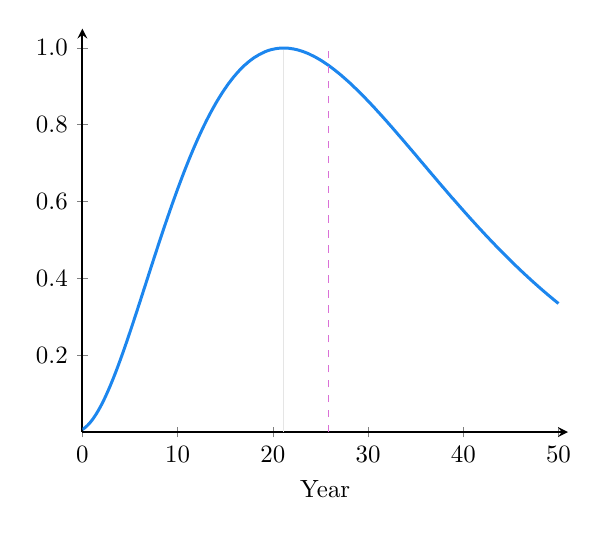
\begin{tikzpicture}[scale=0.9]
		\begin{axis}[axis x line=bottom, axis y line=left, xlabel=Year,
		xtick={0,10,...,50}, ytick={0.2,0.4,...,1.0}, xmax=51, ymax=1.05,
		y tick label style={/pgf/number format/.cd,fixed,fixed zerofill,precision=1,/tikz/.cd}]
		\addplot[DodgerBlue2,very thick,mark=none,domain=0:50,samples=501]
		{0.006738536*exp(0.7*ln(\x+1)/(1-0.7) + \x*ln(0.9))};
		\addplot[lightgray,thin,mark=none]
		coordinates{(21.1,0) (21.1,0.995)} ;
		\addplot[Orchid,thin,dashed,mark=none]
		coordinates{(25.8,0) (25.8,1)} ;
		\end{axis}
		\end{tikzpicture}
	} \qquad
	\subfloat[][$\delta=0.7$, \scriptsize{$\lambda=0.8$, $N=35$, max=9.5, mean=13.4}]{
		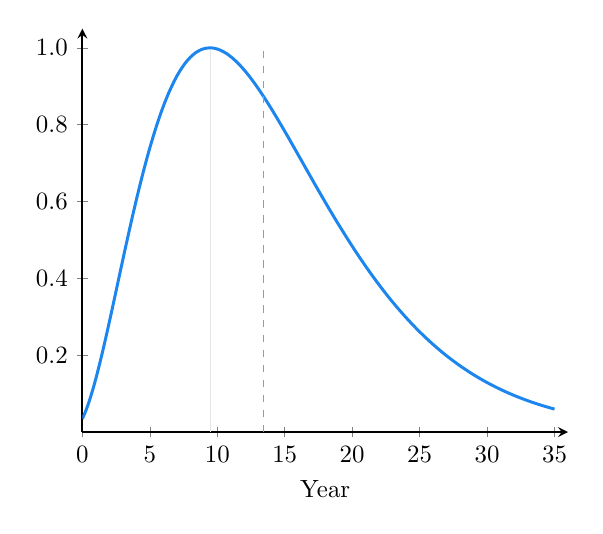
\begin{tikzpicture}[scale=0.9]
		\begin{axis}[axis x line=bottom, axis y line=left, xlabel=Year,
		xtick={0,5,...,35}, ytick={0.2,0.4,...,1.0}, xmax=36, ymax=1.05,
		y tick label style={/pgf/number format/.cd,fixed,fixed zerofill,precision=1,/tikz/.cd}]
		\addplot[DodgerBlue2,very thick,mark=none,domain=0:35,samples=351]
		{0.03450336*exp(0.7*ln(\x+1)/(1-0.7) + \x*ln(0.8))};
		\addplot[lightgray,thin,mark=none]
		coordinates{(9.5,0) (9.5,0.995)} ;
		\addplot[Orchid,thin,dashed,mark=none]
		coordinates{(13.4,0) (13.4,1)} ;
		\end{axis}
		\end{tikzpicture}
	} \\
	\subfloat[][$\delta=0.6$, \scriptsize{$\lambda=0.85$, $N=25$, max=8.2, mean=11.6}]{
		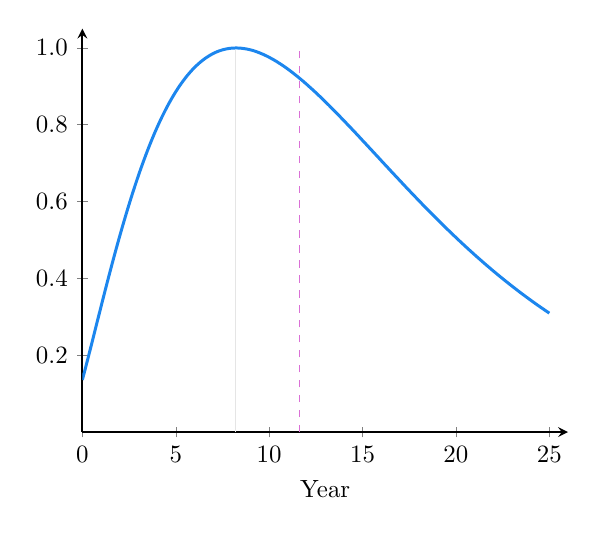
\begin{tikzpicture}[scale=0.9]
		\begin{axis}[axis x line=bottom, axis y line=left, xlabel=Year,
		xtick={0,5,...,25}, ytick={0.2,0.4,...,1.0}, xmax=26, ymax=1.05,
		y tick label style={/pgf/number format/.cd,fixed,fixed zerofill,precision=1,/tikz/.cd}]
		\addplot[DodgerBlue2,very thick,mark=none,domain=0:25,samples=251]
		{0.135856271*exp(0.6*ln(\x+1)/(1-0.6) + \x*ln(0.85))};
		\addplot[lightgray,thin,mark=none]
		coordinates{(8.2,0) (8.2,0.995)} ;
		\addplot[Orchid,thin,dashed,mark=none]
		coordinates{(11.6,0) (11.6,1)} ;
		\end{axis}
		\end{tikzpicture}
	} \qquad
	\subfloat[][$\delta=0.4$, \scriptsize{$\lambda=0.8$, $N=15$, max=2.0, mean=5.4}]{
		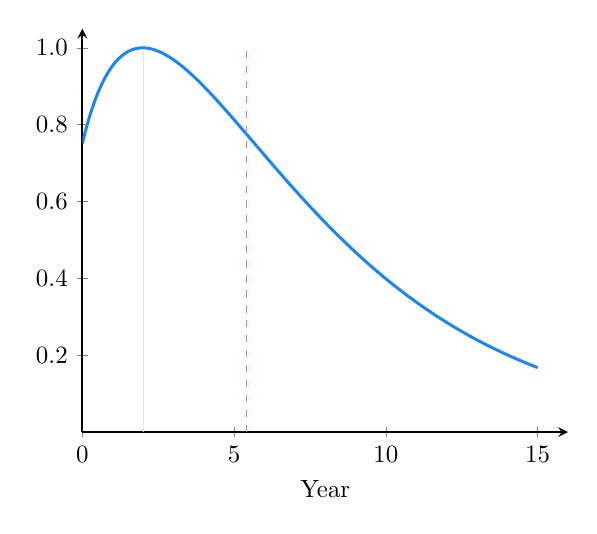
\begin{tikzpicture}[scale=0.9]
		\begin{axis}[axis x line=bottom, axis y line=left, xlabel=Year,
		xtick={0,5,...,15}, ytick={0.2,0.4,...,1.0}, xmax=16, ymax=1.05,
		y tick label style={/pgf/number format/.cd,fixed,fixed zerofill,precision=1,/tikz/.cd}]
		\addplot[DodgerBlue2,very thick,mark=none,domain=0:15,samples=151]
		{0.751167359*exp(0.4*ln(\x+1)/(1-0.4) + \x*ln(0.8))};
		\addplot[lightgray,thin,mark=none]
		coordinates{(2.0,0) (2.0,0.995)} ;
		\addplot[Orchid,thin,dashed,mark=none]
		coordinates{(5.4,0) (5.4,1)} ;
		\end{axis}
		\end{tikzpicture}
	} \\
	\subfloat[][$\delta=0.7$, \scriptsize{$\lambda=0.9$, $N=25$, max=21.1, mean=16.3}]{
		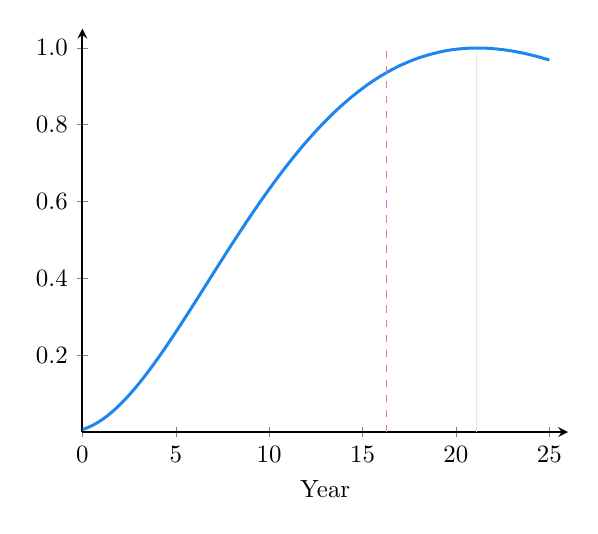
\begin{tikzpicture}[scale=0.9]
		\begin{axis}[axis x line=bottom, axis y line=left, xlabel=Year,
		xtick={0,5,...,25}, ytick={0.2,0.4,...,1.0}, xmax=26, ymax=1.05,
		y tick label style={/pgf/number format/.cd,fixed,fixed zerofill,precision=1,/tikz/.cd}]
		\addplot[DodgerBlue2,very thick,mark=none,domain=0:25,samples=251]
		{0.006738536*exp(0.7*ln(\x+1)/(1-0.7) + \x*ln(0.9))};
		\addplot[lightgray,thin,mark=none]
		coordinates{(21.1,0) (21.1,0.99)} ;
		\addplot[Orchid,thin,dashed,mark=none]
		coordinates{(16.3,0) (16.3,1)} ;
		\end{axis}
		\end{tikzpicture}
	} \qquad
	\subfloat[][$\delta=0.5$, \scriptsize{$\lambda=0.8$, $N=15$, max=3.5, mean=6.3}]{
		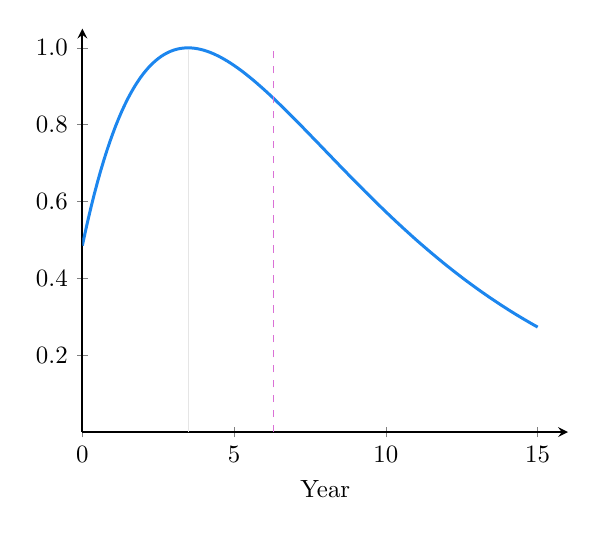
\begin{tikzpicture}[scale=0.9]
		\begin{axis}[axis x line=bottom, axis y line=left, xlabel=Year,
		xtick={0,5,...,15}, ytick={0.2,0.4,...,1.0}, xmax=16, ymax=1.05,
		y tick label style={/pgf/number format/.cd,fixed,fixed zerofill,precision=1,/tikz/.cd}]
		\addplot[DodgerBlue2,very thick,mark=none,domain=0:15,samples=151]
		{0.48525365*exp(0.5*ln(\x+1)/(1-0.5) + \x*ln(0.8))};
		\addplot[lightgray,thin,mark=none]
		coordinates{(3.5,0) (3.5,0.995)} ;
		\addplot[Orchid,thin,dashed,mark=none]
		coordinates{(6.3,0) (6.3,1)} ;
		\end{axis}
		\end{tikzpicture}
	} \\
	\caption{Gamma distribution examples}
	\label{fig:gamDist}
\end{figure}


\chapter{Analytical SAM and GTAP correspondence}
This section describes the accounting framework used by the the model. Two
different accounting frameworks will be described. The first describes the
analytical SAM underlying the model, i.e. how the SAM can be constructed using
the variables of the model. The second describes the links between the model
variables and the initial database as provided by GTAP.\footnote{This refers to
the new standard database, not the 'classic' GTAP database.} The SAM is not a
standard SAM and does not represent the full functionality of the model nor the
underlying database. For example, demand is specified at the Armington level and
the sales tax are collapsed to a single row dimension.

\section{The analytical SAM}

The analytical SAM is the accounting framework that is derived from the
variables of the model. In the absence of a shock, the analytical SAM should
reproduce the input SAM. Table~\ref{tab:AnalSAM} re-produces the analytical SAM.
Below are a few explanatory notes:

\begin{enumerate}
   \item The regional index ($r$) is dropped for most of the expressions except
         when needed, for example in the bilateral trade flows.
   \item The SAM reflects the differentiation between activities and
         commodities. The intersection of the activity rows with the commodity
         columns represents the transformation of domestic production into
         commodities. In the standard version of the model, the matrix is
         diagonal and there is a one-to-one mapping between activities and
         commodities.
   \item The trade rows under the commodity columns represents the bilateral
         imports for region $r$. These are priced at border, i.e. CIF, prices.
         The commodity rows under the trade columns represent bilateral exports
         from region $r$ and are valued at border, i.e. FOB, prices. At the
         global level, the difference between the two matrices represents the
         aggregate value of the trade and transport margins.
   \item Outbound remittances are calculated post-tax. Inbound remittances
         accrue to households.
   \item In the standard GTAP database, most direct taxes are levied on factor
         remuneration. There is no balancing between private and public savings.
         Direct household taxation is calibrated as a balancing item to clear
         the government accounts under the assumption that the deficit is zero.
         This can readily be modified with supplemental data. Direct household
         taxation can be negative, reflecting that net transfers between the
         government and households is positive.
   \item The \texttt{BOP} row under the trade columns represents aggregate
         imports from each region (at border prices). Similarly, the trade rows
         under the \texttt{BOP} column represents the aggregate exports of
         region $r$ towards each region. The \texttt{BOP} accounts reflect the
         full balance of payments. For each region, the sum of exports
         (including the export of trade and transport services) less the sum of
         imports, adjusted by remittances and net capital income,  equals the
         net flow of foreign savings. At the global level, the foreign savings
         cell should be zero.
\end{enumerate}

\begin{landscape}
\begin{table}
\scriptsize
\caption{Analytical SAM}
\label{tab:AnalSAM}
\centering
\rowcolors{2}{TableOdd}{TableEven}
\rowcolors{1}{}{lightblue}
\begin{tabular}{l c c c }
\arrayrulecolor{TableBorder}\specialrule{1pt}{0pt}{0pt}
{} & \bf{\emph{ACT}($a$)} & \bf{\emph{COMM}($i$)}  & \bf{\emph{LAB}($l$)} \\
\arrayrulecolor{TableBorder}\specialrule{1pt}{0pt}{0pt}
\emph{Activities}($a$) & {} & $\mathit{P}_{a,i} \mathit{X}_{a,i}$ &  {} \\
\emph{Commodities}($i$) & $\gamma^{eda}_{i,a}\mathit{PAT}_{i}
    \mathit{XA}_{i,a}$ & {} & {} \\
\emph{Labor}($l$)                & $\mathit{PF}_{l,a} \mathit{XF}_{l,a} $ & {} & {} \\
\emph{Capital}($\mathit{cap}$)   & $\mathit{PF}_{\mathit{cap},a} \mathit{XF}_{\mathit{cap},a} $ & {} & {} \\
\emph{Land}($\mathit{lnd}$)      & $\mathit{PF}_{\mathit{lnd},a} \mathit{XF}_{\mathit{lnd},a} $ & {} & {} \\
\emph{Nat. Res.}($\mathit{nrs}$) & $\mathit{PF}_{\mathit{nrs},a} \mathit{XF}_{\mathit{nrs},a} $ & {} & {} \\
\emph{Nat. Res.}($\mathit{wat}$) & $\mathit{PF}_{\mathit{wat},a} \mathit{XF}_{\mathit{nrs},a} $ & {} & {} \\
\emph{Indirect tax}              & $\sum_i{\tau^a_{i,a} \gamma^{eda}_{i,a} \mathit{PAT}_i \mathit{XA}_{i,a}}$ & {} & {} \\
\emph{Production tax}            & {} & {$\sum_a{\tau^p_{a,i} \mathit{P}_{a,i} \mathit{X}_{a,i}}$} & {} \\
\emph{Factor taxes}              & $ \sum_f{\tau^v_{f,a} \mathit{PF}_{l,a} \mathit{XF}_{f,a} } $ & {} & {} \\
\emph{Import tax} & {} &
$\sum_s{\tau^{m}_{s,i,r}\mathit{PWM}_{s,i,r} \mathit{XW}^d_{s,i,r}} $& {} \\
\emph{Export tax} & {} &
  $\sum_d{\tau^{e}_{r,i,d}\mathit{PE}_{r,i,d} \mathit{XW}^s_{r,i,d}} $& {} \\
\emph{Direct tax} & {} & {} & $\sum_a{\kappa^f_{l,a}\mathit{PF}_{l,a} \mathit{XF}_{l,a}}$ \\
\emph{Household}  & {} & {} &
   $\sum_a{(1-\kappa^f_{l,a})\mathit{PF}_{l,a}\mathit{XF}_{l,a}}
   - \sum_d{\mathit{Remit}_{d,l,r}}$ \\
\emph{Government}         & {} & {} & {} \\
\emph{Investment}         & {} & {} & {} \\
\emph{Depreciation}         & {} & {} & {} \\
\emph{Trade margins}      & {} & {} & {} \\
\emph{Trade}($s$)         & {} & $\mathit{PWM}_{s,i,r}
   \mathit{XW}^d_{s,i,r}$ & {} \\
\emph{Balance of payments} & {} & {} & ${\sum_d{\mathit{Remit}_{d,l,r}}}$ \\
\arrayrulecolor{TableBorder}\specialrule{1pt}{0pt}{0pt}
\end{tabular}
\end{table}
\end{landscape}

\begin{landscape}
\begin{table}
\scriptsize
\caption*{Table~\ref{tab:AnalSAM} Analytical SAM, ctd.}
\centering
\rowcolors{2}{TableOdd}{TableEven}
\rowcolors{1}{}{lightblue}
\begin{tabular}{l c c c c}
\arrayrulecolor{TableBorder}\specialrule{1pt}{0pt}{0pt}
{} & \bf{\emph{CAP}} & \bf{\emph{LND}} & \bf{\emph{NRS}} & \bf{\emph{WAT}} \\
\arrayrulecolor{TableBorder}\specialrule{1pt}{0pt}{0pt}
\emph{Activities}($a$)            & {} & {} & {} & {} \\
\emph{Commodities}($i$)          & {} & {} & {} & {} \\
\emph{Labor}($l$)                 & {} & {} & {} & {} \\
\emph{Capital}($\mathit{cap}$)   & {} & {} & {} & {} \\
\emph{Land}($\mathit{lnd}$)       & {} & {} & {} & {} \\
\emph{Nat. Res.}($\mathit{nrs}$) & {} & {} & {} & {} \\
\emph{Nat. Res.}($\mathit{wat}$)  & {} & {} & {} & {} \\
\emph{Indirect tax}   & {} & {} & {} & {} \\
\emph{Production tax}  & {} & {} & {} & {} \\
\emph{Factor taxes}   & {} & {} & {} & {} \\
\emph{Import tax}      & {} & {} & {} & {} \\
\emph{Export tax}     & {} & {} & {} & {} \\
\emph{Direct tax} &
   {$\displaystyle \sum_a{\kappa^f_{\mathit{cap},a}\mathit{PF}_{\mathit{cap},a} \mathit{XF}_{\mathit{cap},a}}$} &
   {$\displaystyle \sum_a{\kappa^f_{\mathit{lnd},a}\mathit{PF}_{\mathit{lnd},a} \mathit{XF}_{\mathit{lnd},a}}$} &
   {$\displaystyle \sum_a{\kappa^f_{\mathit{nrs},a}\mathit{PF}_{\mathit{nrs},a} \mathit{XF}_{\mathit{nrs},a}}$} &
   {$\displaystyle \sum_a{\kappa^f_{\mathit{wat},a}\mathit{PF}_{\mathit{wat},a} \mathit{XF}_{\mathit{wat},a}}$} \\
\emph{Household}
   & {$\displaystyle \begin{array}{c} \sum_a{(1-\kappa^f_{\mathit{cap},a})\mathit{PF}_{\mathit{cap},a} \mathit{XF}_{\mathit{cap},a}} \\
            - \mathit{YQTF}\\ \end{array}$}
   & {$\displaystyle \sum_a{(1-\kappa^f_{\mathit{lnd},a})\mathit{PF}_{\mathit{lnd},a} \mathit{XF}_{\mathit{lnd},a}}$}
   & {$\displaystyle \sum_a{(1-\kappa^f_{\mathit{nrs},a})\mathit{PF}_{\mathit{nrs},a} \mathit{XF}_{\mathit{nrs},a}}$}
   & {$\displaystyle \sum_a{(1-\kappa^f_{\mathit{wat},a})\mathit{PF}_{\mathit{wat},a} \mathit{XF}_{\mathit{wat},a}}$} \\
\emph{Government}     & {} & {} & {} & {} \\
\emph{Investment}     & {} & {} & {} & {} \\
\emph{Depreciation}   & {} & {} & {} & {} \\
\emph{Trade margins}  & {} & {} & {} & {} \\
\emph{Trade}($s$)     & {} & {} & {} & {} \\
\emph{Balance of payments} & {$\mathit{YQTF}_r$} & {} & {} & {} \\
\arrayrulecolor{TableBorder}\specialrule{1pt}{0pt}{0pt}
\end{tabular}
\end{table}
\end{landscape}

\begin{landscape}
\begin{table}
\scriptsize
\caption*{Table~\ref{tab:AnalSAM} Analytical SAM, ctd.}
\centering
\rowcolors{2}{TableOdd}{TableEven}
\rowcolors{1}{}{lightblue}
\begin{tabular}{l c c c c c c}
\arrayrulecolor{TableBorder}\specialrule{1pt}{0pt}{0pt}
{} & \bf{\emph{ITX}} & \bf{\emph{PTX}} & \bf{\emph{VTX}} & \bf{\emph{MTX}} & \bf{\emph{ETX}} & \bf{\emph{DTX}} \\
\arrayrulecolor{TableBorder}\specialrule{1pt}{0pt}{0pt}
\emph{Activities}($a$)            & {} & {} & {} & {} & {} & {} \\
\emph{Commodities}($i$)          & {} & {} & {} & {} & {} & {} \\
\emph{Labor}($l$)                 & {} & {} & {} & {} & {} & {} \\
\emph{Capital}($\mathit{cap}$)   & {} & {} & {} & {} & {} & {} \\
\emph{Land}($\mathit{lnd}$)       & {} & {} & {} & {} & {} & {} \\
\emph{Nat. Res.}($\mathit{nrs}$) & {} & {} & {} & {} & {} & {} \\
\emph{Nat. Res.}($\mathit{wat}$)  & {} & {} & {} & {} & {} & {} \\
\emph{Indirect tax}   & {} & {} & {} & {} & {} & {} \\
\emph{Production tax}  & {} & {} & {} & {} & {} & {} \\
\emph{Factor taxes}   & {} & {} & {} & {} & {} & {} \\
\emph{Import tax}      & {} & {} & {} & {} & {} & {} \\
\emph{Export tax}     & {} & {} & {} & {} & {} & {} \\
\emph{Direct tax}      & {} & {} & {} & {} & {} & {} \\
\emph{Household}      & {} & {} & {} & {} & {} & {} \\
\emph{Government}
   & {$\mathit{YGOV}_{\mathit{itx}}$}
   & {$\mathit{YGOV}_{\mathit{ptx}}$}
   & {$\mathit{YGOV}_{\mathit{vtx}}$}
   & {$\mathit{YGOV}_{\mathit{mtx}}$}
   & {$\mathit{YGOV}_{\mathit{etx}}$}
   & {$\mathit{YGOV}_{\mathit{dtx}}$} \\
\emph{Investment}     & {} & {} & {} & {} & {} & {} \\
\emph{Depreciation}    & {} & {} & {} & {} & {} & {} \\
\emph{Trade margins}  & {} & {} & {} & {} & {} & {} \\
\emph{Trade}($s$)      & {} & {} & {} & {} & {} & {} \\
\emph{Balance of payments} & {} & {} & {} & {} & {} & {} \\
\arrayrulecolor{TableBorder}\specialrule{1pt}{0pt}{0pt}
\end{tabular}
\end{table}
\end{landscape}

\begin{landscape}
\begin{table}
\scriptsize
\caption*{Table~\ref{tab:AnalSAM} Analytical SAM, ctd.}
\centering
\rowcolors{2}{TableOdd}{TableEven}
\rowcolors{1}{}{lightblue}
\begin{tabular}{ l c c c c }
\arrayrulecolor{TableBorder}\specialrule{1pt}{0pt}{0pt}
{} & \bf{\emph{HHD}} & \bf{\emph{GOV}} & \bf{\emph{INV}} & \bf{\emph{DEPR}} \\
\arrayrulecolor{TableBorder}\specialrule{1pt}{0pt}{0pt}
\emph{Activities}($a$)            & {} & {} & {} & {} \\
\emph{Commodities}($i$)
   & {$\gamma^{eda}_{i,h}\mathit{PAT}^a_{i} \mathit{XA}_{i,h}$}
   & {$\gamma^{eda}_{i,\mathit{gov}}\mathit{PAT}^a_{i} \mathit{XA}_{i,\mathit{gov}}$}
   & {$\gamma^{eda}_{i,\mathit{inv}}\mathit{PA}^a_{i} \mathit{XA}_{i,\mathit{inv}}$}
   & {} \\
\emph{Labor}($l$)                 & {} & {} & {} & {} \\
\emph{Capital}($\mathit{cap}$)   & {} & {} & {} & {} \\
\emph{Land}($\mathit{lnd}$)       & {} & {} & {} & {} \\
\emph{Nat. Res.}($\mathit{nrs}$) & {} & {} & {} & {} \\
\emph{Nat. Res.}($\mathit{wat}$)  & {} & {} & {} & {} \\
\emph{Indirect tax}
   & {$\sum_i{\tau^a_{i,\mathit{h}} \gamma^{eda}_{i,h}\mathit{PAT}_i \mathit{XA}_{i,\mathit{h}}}$}
   & {$\sum_i{\tau^a_{i,\mathit{gov}} \gamma^{eda}_{i,\mathit{gov}}\mathit{PAT}_i \mathit{XA}_{i,\mathit{gov}}}$}
   & {$\sum_i{\tau^a_{i,\mathit{inv}} \gamma^{eda}_{i,\mathit{inv}}\mathit{PAT}_i \mathit{XA}_{i,\mathit{inv}}}$}
   & {} \\
\emph{Production tax}      & {} & {} & {} & {} \\
\emph{Factor taxes}        & {} & {} & {} & {} \\
\emph{Import tax}          & {} & {} & {} & {} \\
\emph{Export tax}          & {} & {} & {} & {} \\
\emph{Direct tax}          & {$\kappa^h\mathit{YH}$} & {} & {} & {} \\
\emph{Household}           & {} & {} & {} & {} \\
\emph{Government}          & {} & {} & {} & {} \\
\emph{Investment}          & {$S^h$} & {$S^g$} & {} & {$\mathit{DeprY}$} \\
\emph{Depreciation}        & {$\mathit{DeprY}$} & {} & {} & {} \\
\emph{Trade margins}       & {} & {} & {} & {} \\
\emph{Trade}($s$)          & {} & {} & {} & {} \\
\emph{Balance of payments} & {} & {$\mathit{ODAOut}$} & {} & {} \\
\arrayrulecolor{TableBorder}\specialrule{1pt}{0pt}{0pt}
\end{tabular}
\end{table}
\end{landscape}

\begin{landscape}
\begin{table}
\scriptsize
\caption*{Table~\ref{tab:AnalSAM} Analytical SAM, ctd.}
\centering
\rowcolors{2}{TableOdd}{TableEven}
\rowcolors{1}{}{lightblue}
\begin{tabular}{l c c c }
\arrayrulecolor{TableBorder}\specialrule{1pt}{0pt}{0pt}
{} & \bf{\emph{TMG}($\mathit{fd}$)}  & \bf{\emph{TRD}($\mathit{d}$)}  & \bf{\emph{BOP}} \\
\arrayrulecolor{TableBorder}\specialrule{1pt}{0pt}{0pt}
\emph{Activities}($a$)            & {} & {} & {} \\
\emph{Commodities}($i$)
 & {$\mathit{PDT}_i \mathit{XTT}_i$}
 & {$\sum_d{\mathit{PWE}_{r,i,d} \mathit{XW}_{r,i,d}}$}
 & {} \\
\emph{Labor}($l$)                   & {} & {} & {} \\
\emph{Capital}($\mathit{cap}$)      & {} & {} & {} \\
\emph{Land}($\mathit{lnd}$)         & {} & {} & {} \\
\emph{Nat. Res.}($\mathit{nrs}$)    & {} & {} & {} \\
\emph{Nat. Res.}($\mathit{wat}$)    & {} & {} & {} \\
\emph{Indirect tax}                 & {} & {} & {} \\
\emph{Production tax}               & {} & {} & {} \\
\emph{Factor taxes}                 & {} & {} & {} \\
\emph{Import tax}                   & {} & {} & {} \\
\emph{Export tax}                   & {} & {} & {} \\
\emph{Direct tax}                   & {} & {} & {} \\
\emph{Household}
   & {}
   & {}
   & {$\sum_s{\mathit{Remit}_{r,l,s}} + \mathit{YQHT}_r$} \\
\emph{Government}           & {} & {} & {$\mathit{ODAOut}$} \\
\emph{Investment}
   & {}
   & {}
   & {$\mathit{PW}^{\mathit{sav}} S^f_r$} \\
\emph{Depreciation}         & {} & {} & {} \\
\emph{Trade margins}
   & {}
   & {}
   & {$\sum_i{\mathit{PDT}_{r,i}\mathit{XTT_{r,i}}}$} \\
\emph{Trade}($s$)
   & {}
   & {}
   & {$\sum_d{\sum_i{\mathit{PWE}_{r,i,d} \mathit{XW}_{r,i,d}}}$} \\
\emph{Balance of payments}
   & {} & {$\sum_s{\sum_i{{\mathit{PWM}_{s,i,r} \mathit{XW}_{s,i,r}}}}$} & {} \\
\arrayrulecolor{TableBorder}\specialrule{1pt}{0pt}{0pt}
\end{tabular}
\end{table}
\end{landscape}

\section{Correspondence to GTAP database}

Table~\ref{tab:corrtab} provides the correspondence between the variables in the
GAMS model and the standard GTAP database that is used as the starting basis for
the GTAP model. Note that The GTAP database reflects an Armington structure that
is agent-specific (at the top nest). The model allows for either a national or
agent-specific decomposition of domestic absorption across sources. The
correspondence herein reflects national sourcing. Hence, the domestic/import
split by agent in the GTAP database is aggregated to provide demand at the
Armington level.

\begin{landscape}
\begin{table}
\small
\caption{Correspondence between GAMS model variables and GTAP database}
\label{tab:corrtab}
\centering
\rowcolors{2}{TableOdd}{TableEven}
\rowcolors{1}{}{lightblue}
\begin{tabular}{ l l l c }
\arrayrulecolor{TableBorder}\specialrule{1pt}{0pt}{0pt}
\bf{\emph{GTAP}} & \bf{\emph{GAMS}}  & \bf{\emph{Description}} \\
\arrayrulecolor{TableBorder}\specialrule{1pt}{0pt}{0pt}
{\texttt{VDFB}+\texttt{VIFB}} &
   $\mathit{PAT}_{r,i}\mathit{XA}_{r,i,a}$ &
   {Firms' (Armington) purchases at basic prices} \\
{\texttt{VDFP}+\texttt{VIFP}} &
   $\mathit{PA}_{r,i,a}\mathit{XA}_{r,i,a}$ &
   {Firms' (Armington) purchases at purchaser prices} \\
{\texttt{VDPB}+\texttt{VIPB}} &
   $\mathit{PAT}_{r,i}\mathit{XA}_{r,i,h}$ &
   {Household (Armington) purchases at basic prices} \\
{\texttt{VDPP}+\texttt{VIPP}} &
   $\mathit{PA}_{r,i,h}\mathit{XA}_{r,i,h}$ &
   {Household (Armington) purchases at purchaser prices} \\
{\texttt{VDGB}+\texttt{VIGB}} &
   $\mathit{PAT}_{r,i}\mathit{XA}_{r,i,\mathit{gov}}$ &
   {Government (Armington) purchases at basic prices} \\
{\texttt{VDGP}+\texttt{VIGP}} &
   $\mathit{PA}_{r,i,\mathit{gov}} \mathit{XA}_{r,i,\mathit{gov}}$ &
   \small{Government (Armington) purchases at purchasers prices} \\
{\texttt{VDIB}+\texttt{VIIB}} &
   $\mathit{PAT}_{r,i}\mathit{XA}_{r,i,\mathit{inv}}$ &
   \small{Investment (Armington) purchases at basic prices} \\
{\texttt{VDIP}+\texttt{VIIP}} &
   $\mathit{PA}_{r,i,\mathit{inv}}\mathit{XA}_{r,i,\mathit{inv}}$ &
   \small{Investment (Armington) purchases at purchaser prices} \\
{\texttt{EVFB(f)}} &
   $\mathit{PF}_{r,f,a}\mathit{XF}_{r,f,a}$ &
   {Firms' purchases of factors at basic prices} \\
{\texttt{EVFP(f)}} &
   $\mathit{PF}^p_{r,f,a}\mathit{XF}_{r,f,a}$ &
   {Firms' purchases of factors at purchaser prices} \\
{\texttt{VOS}} &
   $\mathit{PX}_{r,a}\mathit{XP}_{r,a}$ &
   {Value of production at producer cost} \\
{\texttt{MAKB}} &
   $\mathit{P}_{r,a,i}\mathit{X}_{r,a,i}$ &
   {Value of make matrix at basic prices} \\
{\texttt{MAKS}} &
   $\mathit{PP}_{r,a,i}\mathit{X}_{r,a,i}$ &
   {Value of make matrix at suppliers' prices} \\
{\texttt{EVOS(f)}} &
   $(1-\kappa^f_{r,f,a}){\mathit{PF}_{r,f,a}\mathit{XF}_{r,f,a}}$ &
   {After tax factor remuneration} \\
{\texttt{VKB}}  &
   $\mathit{K}^s_{r}$ &
   {Initial capital stock} \\
{\texttt{VDEP}} &
   $\mathit{DeprY}$ &
   {Value of depreciation} \\
{\texttt{VIMB}} &
   $\mathit{PDM}_{s,i,r}\mathit{XW}^d_{s,i,r}$ &
   {Value of bilateral imports tariff inclusive} \\
{\texttt{VCIF}} &
   $\mathit{PWM}_{s,i,r}\mathit{XW}^d_{s,i,r}$ &
   {Value of bilateral imports at border prices} \\
{\texttt{VFOB}} &
   $\mathit{PWE}_{r,i,d}\mathit{XW}^s_{r,i,d}$ &
   {Value of bilateral exports at border prices} \\
{\texttt{VXSB}} &
   $\mathit{PE}_{r,i,d}\mathit{XW}^s_{r,i,d}$ &
   {Value of bilateral exports at producer prices} \\
{\texttt{VST}}  &
   $\mathit{PDT}_{r,m}\mathit{XTT}_{r,m}$ &
   {Domestic exports of trade \& transport services} \\
{\texttt{VTWR}} &
   $\mathit{PTMG}_{m}\mathit{XMG}^m_{m,r,i,d}$ &
   {Value of margins from $r$ to $d$ for good $i$ using mode $m$} \\
{\texttt{POP}}
   & $\mathit{Pop}_{r}$ &
   {Population---millions} \\
\arrayrulecolor{TableBorder}\specialrule{1pt}{0pt}{0pt}
\end{tabular}
\end{table}
\end{landscape}


\chapter{Dimensions of the GTAP database, release 11}
\label{chap:GTAPDim}
\renewcommand{\theequation}{{D-}\arabic{equation}}
\setcounter{equation}{0}
\captionsetup[table]{list=yes}
\begin{table}[ht]
\footnotesize
\caption{Regional dimension of the GTAP database (V11)}
\label{tab:GTAPREG}
\begin{center}
\rowcolors{2}{TableOdd}{TableEven}
\rowcolors{1}{}{lightblue}
\begin{tabular}{m{0.6cm} m{0.9cm} m{13cm} }
\arrayrulecolor{TableBorder}\specialrule{1pt}{0pt}{0pt}
1 & {AUS} & \textbf{Australia} \\
{} & {} & \scriptsize {Australia (aus), Christmas Island (cxr),
Cocos (Keeling) Islands (cck), Heard and McDonald Islands (hmd),
Norfolk Island (nfk)} \\
\hline
2 & {NZL} & \textbf{New Zealand} \\ \hline
3 & {XOC} & \textbf{Rest of Oceania} \\
{} & {} & \scriptsize {American Samoa (asm), Cook Islands (cok), Fiji (fji), French Polynesia (pyf), Guam (gum), Kiribati (kir), Marshall Islands (mhl), Federated States of Micronesia (fsm), Nauru (nau), New Caledonia (ncl), Niue (niu), Northern Mariana Islands (mnp), Palau (plw), Papua New Guinea (png), Pitcairn (pcn), Samoa (wsm), Solomon Islands (slb), Tokelau (tkl), Tonga (ton), Tuvalu (tuv), United States Minor Outlying Islands (umi), Vanuatu (vut), Wallis and Futura Islands (wlf)} \\ \hline
4 & {CHN} & \textbf{China} \\ \hline
5 & {HKG} & \textbf{Hong Kong SAR (hkg)} \\ \hline
6 & {JPN} & \textbf{Japan} \\ \hline
7 & {KOR} & \textbf{Republic of Korea} \\ \hline
8 & {MNG} & \textbf{Mongolia} \\ \hline
9 & {TWN} & \textbf{Taiwan (Province of China)} \\ \hline
10 & {XEA} & \textbf{Rest of East Asia} \\
{} & {} & \scriptsize {Macao SAR (mac), North Korea (prk)} \\ \hline
12 & {KHM} & \textbf{Cambodia} \\ \hline
13 & {IDN} & \textbf{Indonesia} \\ \hline
14 & {LAO} & \textbf{Lao, PDR} \\ \hline
15 & {MYS} & \textbf{Malaysia} \\ \hline
16 & {PHL} & \textbf{Philippines} \\ \hline
17 & {SGP} & \textbf{Singapore} \\ \hline
18 & {THA} & \textbf{Thailand} \\ \hline
19 & {VNM} & \textbf{Vietnam} \\ \hline
20 & {XSE} & \textbf{Rest of Southeast Asia} \\
{} & {} & \scriptsize {Myanmar (mmr), Timor-Leste (tmp)} \\ \hline
\specialrule{1pt}{0pt}{0pt}
\end{tabular}
\end{center}
\end{table}

%\addtocounter{table}{1}

\captionsetup[table]{list=no}
\begin{table}[ht]\ContinuedFloat
\caption{Regional dimension of the GTAP database (cont.)}
\footnotesize
\begin{center}
\rowcolors{2}{TableOdd}{TableEven}
\rowcolors{1}{}{lightblue}
\begin{tabular}{m{0.6cm} m{0.9cm} m{13cm} }
\arrayrulecolor{TableBorder}\specialrule{1pt}{0pt}{0pt}
21 & {AFG} & \textbf{Afghanistan} \\ \hline
22 & {BGD} & \textbf{Bangladesh} \\ \hline
23 & {IND} & \textbf{India} \\ \hline
24 & {LKA} & \textbf{Sri Lanka} \\ \hline
25 & {NPL} & \textbf{Nepal} \\ \hline
26 & {PAK} & \textbf{Pakistan} \\ \hline
27 & {XSA} & \textbf{Rest of South Asia} \\
{} & {} & \scriptsize {Bhutan (btn), Maldives (mdv)} \\ \hline
28 & {CAN} & \textbf{Canada} \\ \hline
29 & {USA} & \textbf{United States} \\ \hline
30 & {MEX} & \textbf{Mexico} \\ \hline
31 & {XNA} & \textbf{Rest of North America} \\
{} & {} & \scriptsize {Bermuda (bmu), Greenland (grl), Saint Pierre \& Miquelon (spm)} \\ \hline
32 & {ARG} & \textbf{Argentina} \\ \hline
33 & {BOL} & \textbf{Bolivia} \\ \hline
34 & {BRA} & \textbf{Brazil} \\ \hline
35 & {CHL} & \textbf{Chile} \\ \hline
36 & {COL} & \textbf{Colombia} \\ \hline
37 & {ECU} & \textbf{Ecuador} \\ \hline
38 & {PRY} & \textbf{Paraguay} \\ \hline
39 & {PER} & \textbf{Peru} \\ \hline
40 & {URY} & \textbf{Uruguay} \\ \hline
41 & {VEN} & \textbf{Venezuela, Republica Bolivariana de} \\ \hline
42 & {XSM} & \textbf{Rest of South America} \\
{} & {} & \scriptsize {Falkland Islands (flk), French Guiana (guf), Guyana (guy), South Georgia and the South Sandwich Islands (sgs), Suriname (sur)} \\ \hline
43 & {CRI} & \textbf{Costa Rica} \\ \hline
44 & {GTM} & \textbf{Guatemala} \\ \hline
45 & {HND} & \textbf{Honduras} \\ \hline
46 & {NIC} & \textbf{Nicaragua} \\ \hline
47 & {PAN} & \textbf{Panama} \\ \hline
48 & {SLV} & \textbf{El Salvador} \\ \hline
49 & {XCA} & \textbf{Rest of Central America} \\
{} & {} & \scriptsize {Belize (blz)} \\ \hline
50 & {DOM} & \textbf{Dominican Republic} \\ \hline
51 & {JAM} & \textbf{Jamaica} \\ \hline
52 & {HTI} & \textbf{Haiti} \\ \hline
53 & {PRI} & \textbf{Puerto Rico} \\ \hline
54 & {TTO} & \textbf{Trinidad \& Tobago} \\ \hline
55 & {XCB} & \textbf{Caribbean} \\
{} & {} & \scriptsize {Anguilla (aia), Antigua and Barbuda (atg), Aruba (abw), Bahamas (bhs), Barbados (brb), Bonaire, Sint Eustatius and Saba (bes), British Virgin Islands (vgb), Cayman Islands (cym), Cuba (cub), Cura\c{c}ao (cuw), Dominica (dma), Grenada (grd),  Montserrat (msr), Saint Barth\'elemy (blm), Saint Kitts and Nevis (kna), Saint Lucia (lca), Saint Martin (French Part) (maf), Saint Vincent and the Grenadines (vct), Sint Maarten (Dutch part) (sxm), Turks and Caicos Islands (tca), United States Virgin Islands (vir)} \\ \hline
\specialrule{1pt}{0pt}{0pt}
\end{tabular}
\end{center}
\end{table}

%\addtocounter{table}{1}

\captionsetup[table]{list=no}
\begin{table}[ht]\ContinuedFloat
\caption{Regional dimension of the GTAP database (cont.)}
\footnotesize
\begin{center}
\rowcolors{2}{TableOdd}{TableEven}
\rowcolors{1}{}{lightblue}
\begin{tabular}{m{0.6cm} m{0.9cm} m{13cm} }
\arrayrulecolor{TableBorder}\specialrule{1pt}{0pt}{0pt}
56 & {AUT} & \textbf{Austria} \\ \hline
57 & {BEL} & \textbf{Belgium} \\ \hline
58 & {BGR} & \textbf{Bulgaria} \\ \hline
59 & {HRV} & \textbf{Croatia} \\ \hline
60 & {CYP} & \textbf{Cyprus} \\ \hline
61 & {CZE} & \textbf{Czech Republic} \\ \hline
62 & {DNK} & \textbf{Denmark} \\ \hline
63 & {EST} & \textbf{Estonia} \\ \hline
64 & {FIN} & \textbf{Finland} \\
{} & {} & \scriptsize {{\r{A}}land Islands (ala), Finland (fin)} \\ \hline
65 & {FRA} & \textbf{France} \\
{} & {} & \scriptsize {France (fra), Guadeloupe (glp), Martinique (mtq), R\'eunion (reu)} \\ \hline
66 & {DEU} & \textbf{Germany} \\ \hline
67 & {GRC} & \textbf{Greece} \\ \hline
68 & {HUN} & \textbf{Hungary} \\ \hline
69 & {IRL} & \textbf{Ireland} \\ \hline
70 & {ITA} & \textbf{Italy} \\ \hline
71 & {LVA} & \textbf{Latvia} \\ \hline
72 & {LTU} & \textbf{Lithuania} \\ \hline
73 & {LUX} & \textbf{Luxembourg} \\ \hline
74 & {MLT} & \textbf{Malta} \\ \hline
75 & {NLD} & \textbf{Netherlands} \\ \hline
76 & {POL} & \textbf{Poland} \\ \hline
77 & {PRT} & \textbf{Portugal} \\ \hline
78 & {ROU} & \textbf{Romania} \\ \hline
79 & {SVK} & \textbf{Slovakia} \\ \hline
80 & {SVN} & \textbf{Slovenia} \\ \hline
81 & {ESP} & \textbf{Spain} \\ \hline
82 & {SWE} & \textbf{Sweden} \\ \hline
83 & {GBR} & \textbf{United Kingdom} \\ \hline
84 & {NOR} & \textbf{Norway} \\
{} & {} & \scriptsize {Norway (nor), Svalbard and Jan Mayen Islands
(sjm)} \\ \hline
85 & {CHE} & \textbf{Switzerland} \\ \hline
86 & {XEF} & \textbf{Rest of European Free Trade Area (EFTA)} \\
{} & {} & \scriptsize {Iceland (isl), Liechtenstein (lie)} \\ \hline
87 & {ALB} & \textbf{Albania} \\ \hline
88 & {SRB} & \textbf{Serbia} \\ \hline
89 & {BLR} & \textbf{Belarus} \\ \hline
90 & {RUS} & \textbf{Russian Federation} \\ \hline
91 & {UKR} & \textbf{Ukraine} \\ \hline
92 & {XEE} & \textbf{Rest of Eastern Europe} \\
{} & {} & \scriptsize {Moldova (mda)} \\ \hline
93 & {XER} & \textbf{Rest of Europe} \\
{} & {} & \scriptsize {Andorra (and), Bosnia and Herzegovina (bih), Faroe Islands (fro), Gibraltar (gib), Guernsey (ggy),
Holy See (vat), Isle of Man (imn), Jersey (jey), Kosovo (uvk),
Monaco (mco), Montenegro (mne), North Macedonia (mkd), San Marino (smr), Sark (srk)} \\ \hline
\specialrule{1pt}{0pt}{0pt}
\end{tabular}
\end{center}
\end{table}

%\addtocounter{table}{1}

\captionsetup[table]{list=no}
\begin{table}[ht]\ContinuedFloat
\caption{Regional dimension of the GTAP database (cont.)}
\footnotesize
\begin{center}
\rowcolors{2}{TableOdd}{TableEven}
\rowcolors{1}{}{lightblue}
\begin{tabular}{m{0.6cm} m{0.9cm} m{13cm} }
\arrayrulecolor{TableBorder}\specialrule{1pt}{0pt}{0pt}
94 & {KAZ} & \textbf{Kazakhstan} \\ \hline
95 & {KGZ} & \textbf{Kyrgyz Republic} \\ \hline
96 & {TJK} & \textbf{Tajikistan} \\ \hline
97 & {UZB} & \textbf{Uzbekistan} \\ \hline
98 & {XSU} & \textbf{Rest of Former Soviet Union} \\
{} & {} & \scriptsize {Turkmenistan (tkm)} \\ \hline
99 & {ARM} & \textbf{Armenia} \\ \hline
100 & {AZE} & \textbf{Azerbaijan} \\ \hline
101 & {GEO} & \textbf{Georgia} \\ \hline
102 & {BHR} & \textbf{Bahrain} \\ \hline
103 & {IRN} & \textbf{Iran} \\ \hline
104 & {IRQ} & \textbf{Iraq} \\ \hline
105 & {ISR} & \textbf{Israel} \\ \hline
106 & {JOR} & \textbf{Jordan} \\ \hline
107 & {KWT} & \textbf{Kuwait} \\ \hline
108 & {LBN} & \textbf{Lebanon} \\ \hline
109 & {OMN} & \textbf{Oman} \\ \hline
110 & {PSE} & \textbf{Palestine} \\ \hline
111 & {QAT} & \textbf{Qatar} \\ \hline
112 & {SAU} & \textbf{Saudi Arabia} \\ \hline
113 & {SYR} & \textbf{Syrian Arab Republic} \\ \hline
114 & {TUR} & \textbf{T\"urkiye} \\ \hline
115 & {ARE} & \textbf{United Arab Emirates} \\ \hline
116 & {XWS} & \textbf{Rest of Western Asia} \\
{} & {} & \scriptsize {Republic of Yemen (yem)} \\ \hline
117 & {DZA} & \textbf{Algeria} \\ \hline
118 & {EGY} & \textbf{Egypt} \\ \hline
119 & {MAR} & \textbf{Morocco} \\ \hline
120 & {TUN} & \textbf{Tunisia} \\ \hline
121 & {XNF} & \textbf{Rest of North Africa} \\
{} & {} & \scriptsize {Libya (lby)} \\ \hline
\specialrule{1pt}{0pt}{0pt}
\end{tabular}
\end{center}
\end{table}

%\addtocounter{table}{1}

\captionsetup[table]{list=no}
\begin{table}[ht]\ContinuedFloat
\caption{Regional dimension of the GTAP database (cont.)}
\footnotesize
\begin{center}
\rowcolors{2}{TableOdd}{TableEven}
\rowcolors{1}{}{lightblue}
\begin{tabular}{m{0.6cm} m{0.9cm} m{13cm} }
\arrayrulecolor{TableBorder}\specialrule{1pt}{0pt}{0pt}
122 & {BEN} & \textbf{Benin} \\ \hline
123 & {BFA} & \textbf{Burkina Faso} \\ \hline
124 & {CMR} & \textbf{Cameroon} \\ \hline
125 & {CIV} & \textbf{C\^ote d'Ivoire} \\ \hline
126 & {GHA} & \textbf{Ghana} \\ \hline
127 & {GIN} & \textbf{Guinea} \\ \hline
128 & {MLI} & \textbf{Mali} \\ \hline
129 & {NER} & \textbf{Niger} \\
130 & {NGA} & \textbf{Nigeria} \\
131 & {SEN} & \textbf{Senegal} \\ \hline
132 & {TGO} & \textbf{Togo} \\
133 & {XWF} & \textbf{Rest of Western Africa} \\ \hline
{} & {} & \scriptsize {Cape Verde (cpv), Gambia, The (gmb), Guinea-Bissau (gnb), Liberia (lbr), Mauritania (mrt), Saint Helena (shn), Sierra Leone (sle)} \\ \hline
134 & {CAF} & \textbf{Central African Republic} \\ \hline
135 & {TCD} & \textbf{Chad} \\ \hline
136 & {COG} & \textbf{Congo} \\ \hline
137 & {COD} & \textbf{Democratic Republic of the Congo} \\ \hline
138 & {GNQ} & \textbf{Equatorial Guinea} \\ \hline
139 & {GAB} & \textbf{Gabon} \\ \hline
140 & {XAC} & \textbf{South-Central Africa} \\
{} & {} & \scriptsize {Angola (ago), S\~ao Tom\'e \& Pr\'incipe (stp)} \\ \hline
141 & {COM} & \textbf{Comoros} \\ \hline
142 & {ETH} & \textbf{Ethiopia} \\ \hline
143 & {KEN} & \textbf{Kenya} \\ \hline
144 & {MDG} & \textbf{Madagascar} \\ \hline
145 & {MWI} & \textbf{Malawi} \\ \hline
146 & {MUS} & \textbf{Mauritius} \\ \hline
147 & {MOZ} & \textbf{Mozambique} \\ \hline
148 & {RWA} & \textbf{Rwanda} \\ \hline
149 & {SDN} & \textbf{Sudan} \\ \hline
150 & {TZA} & \textbf{Tanzania} \\ \hline
151 & {UGA} & \textbf{Uganda} \\ \hline
152 & {ZMB} & \textbf{Zambia} \\ \hline
153 & {ZWE} & \textbf{Zimbabwe} \\ \hline
154 & {XEC} & \textbf{Rest of Eastern Africa} \\
{} & {} & \scriptsize {Burundi (bdi), Djibouti (dji), Eritrea (eri), Mayotte (myt), Seychelles Islands (syc), Somalia (som), South Sudan (ssd)} \\ \hline
155 & {BWA} & \textbf{Botswana} \\ \hline
156 & {SWZ} & \textbf{Eswatini} \\ \hline
157 & {NAM} & \textbf{Namibia} \\ \hline
158 & {ZAF} & \textbf{South Africa} \\ \hline
159 & {XSC} & \textbf{Rest of South African Customs Union} \\
{} & {} & \scriptsize {Lesotho (lso)} \\ \hline
160 & {XTW} & \textbf{Rest of the World} \\
{} & {} & \scriptsize {Antarctica (ata), Bouvet Island (bvt), British Indian Ocean Territory (iot), French Southern Territories (atf)} \\
\specialrule{1pt}{0pt}{0pt}
\end{tabular}
\end{center}
\end{table}

\clearpage
Table~\ref{tab:GTAPCOMM} provides the standard set of commodities
in the GTAP Data Base. In the standard database, these are the
same as the set of activities. The standard commodity subsets are:

\begin{itemize}
    \item \texttt{MARG}: \texttt{OTP}, \texttt{WTP}, \texttt{ATP}
   \item \texttt{ERG }: \texttt{COA}, \texttt{OIL}, \texttt{GAS}, \texttt{P\_C}, \texttt{ELY}, \texttt{GDT}
    \item \texttt{FUEL}: \texttt{COA}, \texttt{OIL}, \texttt{GAS}, \texttt{P\_C}, \texttt{GDT}
\end{itemize}

\captionsetup[table]{list=yes}
\begin{table}[ht]
\footnotesize
\caption{Commodity dimension of the GTAP database (V11)}
\label{tab:GTAPCOMM}
\begin{center}
\rowcolors{2}{TableOdd}{TableEven}
\rowcolors{1}{}{lightblue}
\begin{tabular}{m{0.6cm} m{0.9cm} m{13cm} }
\arrayrulecolor{TableBorder}\specialrule{1pt}{0pt}{0pt}
  1 & {PDR} & \textbf{Paddy rice} \\ \hline
  2 & {WHT} & \textbf{Wheat}\\ \hline
  3 & {GRO} & \textbf{Cereal grains nec}\\ \hline
  4 & {V\_F} & \textbf{Vegetables, fruit, nuts}\\ \hline
  5 & {OSD} & \textbf{Oil seeds}\\ \hline
  6 & {C\_B} & \textbf{Sugar cane, sugar beet}\\ \hline
  7 & {PFB} & \textbf{Plant-based fibers}\\ \hline
  8 & {OCR} & \textbf{Crops nec}\\ \hline
  9 & {CTL} & \textbf{Bovine cattle, sheep and goats, horses}\\ \hline
 10 & {OAP} & \textbf{Animal products nec}\\ \hline
 11 & {RMK} & \textbf{Raw milk}\\ \hline
 12 & {WOL} & \textbf{Wool, silk-worm cocoons}\\ \hline
 13 & {FRS} & \textbf{Forestry}\\ \hline
 14 & {FSH} & \textbf{Fishing}\\ \hline
 15 & {COA} & \textbf{Coal}\\ \hline
 16 & {OIL} & \textbf{Oil}\\ \hline
 17 & {GAS} & \textbf{Gas}\\ \hline
 18 & {OXT} & \textbf{Other Extraction (formerly omn Minerals nec)}\\ \hline
 19 & {CMT} & \textbf{Bovine meat products}\\ \hline
 20 & {OMT} & \textbf{Meat products nec}\\ \hline
 21 & {VOL} & \textbf{Vegetable oils and fats}\\ \hline
 22 & {MIL} & \textbf{Dairy products}\\ \hline
 23 & {PCR} & \textbf{Processed rice}\\ \hline
 24 & {SGR} & \textbf{Sugar}\\ \hline
 25 & {OFD} & \textbf{Food products nec}\\ \hline
 26 & {B\_T} & \textbf{Beverages and tobacco products}\\ \hline
 27 & {TEX} & \textbf{Textiles}\\ \hline
 28 & {WAP} & \textbf{Wearing apparel}\\ \hline
 29 & {LEA} & \textbf{Leather products}\\ \hline
 30 & {LUM} & \textbf{Wood products}\\ \hline
 31 & {PPP} & \textbf{Paper products, publishing}\\ \hline
 32 & {P\_C} & \textbf{Petroleum, coal products}\\ \hline
 33 & {CHM} & \textbf{Chemical products}\\ \hline
 34 & {BPH} & \textbf{Basic pharmaceutical products}\\ \hline
 35 & {RPP} & \textbf{Rubber and plastic products}\\ \hline
\specialrule{1pt}{0pt}{0pt}
\end{tabular}
\end{center}
\end{table}

%\addtocounter{table}{1}

\captionsetup[table]{list=no}
\begin{table}[ht]\ContinuedFloat
\footnotesize
\caption{Commodity dimension of the GTAP database (cont.)}
\begin{center}
\rowcolors{2}{TableOdd}{TableEven}
\rowcolors{1}{}{lightblue}
\begin{tabular}{m{0.6cm} m{0.9cm} m{13cm} }
\arrayrulecolor{TableBorder}\specialrule{1pt}{0pt}{0pt}
 36 & {NMM} & \textbf{Mineral products nec}\\ \hline
 37 & {I\_S} & \textbf{Ferrous metals}\\ \hline
 38 & {NFM} & \textbf{Metals nec}\\ \hline
 39 & {FMP} & \textbf{Metal products}\\ \hline
 40 & {ELE} & \textbf{Computer, electronic and optical products}\\ \hline
 41 & {EEQ} & \textbf{Electrical equipment}\\ \hline
 42 & {OME} & \textbf{Machinery and equipment nec}\\ \hline
 43 & {MVH} & \textbf{Motor vehicles and parts}\\ \hline
 44 & {OTN} & \textbf{Transport equipment nec}\\ \hline
 45 & {OMF} & \textbf{Manufactures nec}\\ \hline
 46 & {ELY} & \textbf{Electricity}\\ \hline
 47 & {GDT} & \textbf{Gas manufacture, distribution}\\ \hline
 48 & {WTR} & \textbf{Water}\\ \hline
 49 & {CNS} & \textbf{Construction}\\ \hline
 50 & {TRD} & \textbf{Trade}\\ \hline
 51 & {AFS} & \textbf{Accommodation, Food and service activities}\\ \hline
 52 & {OTP} & \textbf{Transport nec}\\ \hline
 53 & {WTP} & \textbf{Water transport}\\ \hline
 54 & {ATP} & \textbf{Air transport}\\ \hline
 55 & {WHS} & \textbf{Warehousing and support activities}\\ \hline
 56 & {CMN} & \textbf{Communication}\\ \hline
 57 & {OFI} & \textbf{Financial services nec}\\ \hline
 58 & {INS} & \textbf{Insurance (formerly isr)}\\ \hline
 59 & {RSA} & \textbf{Real estate activities}\\ \hline
 60 & {OBS} & \textbf{Business services nec}\\ \hline
 61 & {ROS} & \textbf{Recreational and other services}\\ \hline
 62 & {OSG} & \textbf{Public Administration and defense}\\ \hline
 63 & {EDU} & \textbf{Education}\\ \hline
 64 & {HHT} & \textbf{Human health and social work activities}\\ \hline
 65 & {DWE} & \textbf{Dwellings}\\ \hline
\specialrule{1pt}{0pt}{0pt}
\end{tabular}
\end{center}
\end{table}

\clearpage

The power-version of the GTAP database splits the standard
electricity sector (\texttt{'ELY'}) into 12 electricity-based
activities---11 of which are different power technologies with
differentiated cost structures and 1 activity for transmission
and distribution. The database assumes full diagonality of the
power structure 'make' matrix. A typical model implementation
is likely to keep the differentiated cost structures but
collapse demand to a single electricity commodity.\footnote{The 12 power activities are added to the \texttt{ERG} subset.}

\captionsetup[table]{list=yes}
\begin{table}[ht]
\footnotesize
\caption{Additional dimensions of the power database (V11)}
\label{tab:GTAPPOW}
\begin{center}
\rowcolors{2}{TableOdd}{TableEven}
\rowcolors{1}{}{lightblue}
\begin{tabular}{m{0.6cm} m{3.0cm} m{11.0cm} }
\arrayrulecolor{TableBorder}\specialrule{1pt}{0pt}{0pt}
  1 & {TND} & \textbf{Electricity transmission and distribution}\\ \hline
  2 & {NUCLEARBL} & \textbf{Nuclear power}\\ \hline
  3 & {COALBL} & \textbf{Coal power baseload}\\ \hline
  4 & {GASBL} & \textbf{Gas power baseload}\\ \hline
  5 & {WINDBL} & \textbf{Wind power}\\ \hline
  6 & {HYDROBL} & \textbf{Hydro power baseload}\\ \hline
  7 & {OILBL} & \textbf{Oil power baseload}\\ \hline
  8 & {OTHERBL} & \textbf{Other baseload}\\ \hline
  9 & {GASP} & \textbf{Gas power peakload}\\ \hline
 10 & {HYDROP} & \textbf{Hydro power peakload}\\ \hline
 11 & {OILP} & \textbf{Oil power peakload}\\ \hline
 12 & {SOLARP} & \textbf{Solar power}\\ \hline
\specialrule{1pt}{0pt}{0pt}
\end{tabular}
\end{center}
\end{table}

The standard version of GTAP has 8 endowments or factors of production---of which
5 are labor types. The first three labor types in Table~\ref{tab:GTAPENDOW}
are typically associated with \emph{unskilled} labor
and the remaining two would therefore be designated \emph{skilled}
labor.\footnote{\cite{WalmsleyCarrico2016}.}
It should be noted that in the default configuration, land payments are only
attributed in the agricultural sectors---both crops and livestock---but not
forestry. Natural resource payments are available for
forestry (\texttt{frs}), fisheries (\texttt{fsh}), coal mining (\texttt{coa}),
oil and gas extraction (\texttt{oil} and \texttt{gas}) and other mining extraction (\texttt{oxt}).

\captionsetup[table]{list=yes}
\begin{table}[ht]
\footnotesize
\caption{GTAP endowments (V11)}
\label{tab:GTAPENDOW}
\begin{center}
\rowcolors{2}{TableOdd}{TableEven}
\rowcolors{1}{}{lightblue}
\begin{tabular}{m{0.6cm} m{3.0cm} m{11.0cm} }
\arrayrulecolor{TableBorder}\specialrule{1pt}{0pt}{0pt}
  1 & {TECH\_ASPROS} & \textbf{Technical and professional workers}\\ \hline
  2 & {CLERKS} & \textbf{Clerical workers}\\ \hline
  3 & {SERVICE\_SHOP} & \textbf{Service shop}\\ \hline
  4 & {OFF\_MGR\_PROS} & \textbf{Management}\\ \hline
  5 & {AG\_OTHLOWSK} & \textbf{Agriculture and other low-skill workers}\\ \hline
  6 & {CAPITAL} & \textbf{Capital}\\ \hline
  7 & {LAND} & \textbf{Land}\\ \hline
  8 & {NATLRES} & \textbf{Natural resources}\\ \hline
\specialrule{1pt}{0pt}{0pt}
\end{tabular}
\end{center}
\end{table}

Table~\ref{tab:GTAPGHG} provides the definitions
for the greenhouse (GHG) and non-greenhouse gases.
The set \texttt{EM} incorporates all air emissions.
The set \texttt{EMN} incorporates all air emissions with
the exception of \COT{}.
The set \texttt{GHG} includes the four greenhouse gases
(\COT{}, $\textrm{CH}_4$, $\textrm{N}_2\textrm{O}$ and \texttt{FGAS}).
The set \texttt{NCO2} represents the greenhouse gases except \COT{}.
The set \texttt{NGHG} includes all non-greenhouse gases.

\captionsetup[table]{list=yes}
\begin{table}[h]
\footnotesize
\caption{Air emissions}
\label{tab:GTAPGHG}
\begin{center}
\rowcolors{2}{TableOdd}{TableEven}
\rowcolors{1}{}{lightblue}
\begin{tabular}{m{0.6cm} m{3.0cm} m{11.0cm} }
\arrayrulecolor{TableBorder}\specialrule{1pt}{0pt}{0pt}
  1 & {CO2}  & \textbf{Carbon dioxide} \\ \hline
  2 & {CH4}  & \textbf{Methane}\\ \hline
  3 & {N2O}  & \textbf{Nitrous oxide}\\ \hline
  4 & {FGAS}  & \textbf{Fluorinated gases }\\ \hline
4 &  C2F6  & \textbf{Hexafluoroethane} (PFC-116, $\textnormal{C}_2\textnormal{F}_6$) \\ \hline
5 &  C3F8  & \textbf{Octafluoropropane} (PFC-218, $\textnormal{C}_3\textnormal{F}_8$) \\ \hline
6 &  C4F10  & \textbf{Perfluorobutane} (PFC-31-10, $\textnormal{C}_4\textnormal{F}_{10}$) \\ \hline
7 &  C5F12  & \textbf{Perfluoropentane} (PFC-41-12, $\textnormal{C}_5\textnormal{F}_{12}$) \\ \hline
8 &  C6F14  & \textbf{Perfluorohexane} (PFC-51-14, $\textnormal{C}_6\textnormal{F}_{14}$) \\ \hline
9 & cC4F8  & \textbf{Octafluorocyclobutane} (PFC-318, $\textnormal{C}_4\textnormal{F}_{8}$) \\ \hline
10 &  CF4  & \textbf{Carbon tetrafluoride} (PFC-14, $\textnormal{C}\textnormal{F}_{4}$) \\ \hline
11 &  HCFC141b  & \textbf{1,1-Dichloro-1-fluoroethane} ($\textnormal{C}_2\textnormal{H}_3\textnormal{Cl}_2\textnormal{F}$) \\ \hline
12 &  HCFC142b  & \textbf{1-Chloro-1,1-difluoroethane} ($\textnormal{C}_2\textnormal{H}_3\textnormal{ClF}_2$) \\ \hline
13 &  HFC125  & \textbf{Pentafluoroethane} ($\textnormal{C}_2\textnormal{H}\textnormal{F}_5$) \\ \hline
14 &  HFC134  & \textbf{1,1,2,2-Tetrafluoroethane} ($\textnormal{C}_2\textnormal{H}_2\textnormal{F}_4$) \\ \hline
15 &  HFC134a  & \textbf{1,1,1,2-Tetrafluoroethane} ($\textnormal{C}_2\textnormal{H}_2\textnormal{F}_4$) \\ \hline
16 &  HFC143  & \textbf{1,1,2-Trifluoroethane} ($\textnormal{C}_2\textnormal{H}_3\textnormal{F}_3$) \\ \hline
17 &  HFC143a  & \textbf{1,1,1-Trifluoroethane} ($\textnormal{C}_2\textnormal{H}_3\textnormal{F}_3$) \\ \hline
18 &  HFC152a  & \textbf{1,1-Difluoroethane} ($\textnormal{C}_2\textnormal{H}_4\textnormal{F}_2$) \\ \hline
19 &  HFC227ea  & \textbf{1,1,1,2,3,3,3-Heptafluoropropane} ($\textnormal{C}_3\textnormal{HF}_7$) \\ \hline
20 &  HFC23  & \textbf{Trifluoromethane} ($\textnormal{CHF}_3$) \\ \hline
21 &  HFC236fa  & \textbf{1,1,1,3,3,3-Hexafluoropropane} ($\textnormal{C}_3\textnormal{H}_2\textnormal{F}_6$) \\ \hline
22 &  HFC245fa  & \textbf{1,1,1,3,3-Pentafluoropropane} ($\textnormal{C}_3\textnormal{H}_3\textnormal{F}_5$) \\ \hline
23 &  HFC32  & \textbf{Difluoromethane} ($\textnormal{C}\textnormal{H}_2\textnormal{F}_2$) \\ \hline
24 &  HFC365mfc  & \textbf{1,1,1,3,3-Pentafluorobutane} ($\textnormal{C}_4\textnormal{H}_5\textnormal{F}_5$) \\ \hline
25 &  HFC41  & \textbf{Fluoromethane} ($\textnormal{C}\textnormal{H}_3\textnormal{F}$) \\ \hline
26 &  HFC4310mee  & \textbf{1,1,1,2,2,3,4,5,5,5-Decafluoropentane} ($\textnormal{C}_5\textnormal{H}_2\textnormal{F}_{10}$) \\ \hline
27 &  NF3  & \textbf{Nitrogen trifluoride} ($\textnormal{NF}_3$) \\ \hline
28 &  SF6  & \textbf{Sulfur hexafluoride} ($\textnormal{SF}_6$) \\ \hline
 29 & BC     & \textbf{Black carbon} \\ \hline
   30 & CO     & \textbf{Carbon monoxide} \\ \hline
  31 & NH3    & \textbf{Ammonia} \\ \hline
   32 & NMVOC   & \textbf{Non-methane volatile organic compounds} \\ \hline
   33 & NOX    & \textbf{Nitrogen oxides} \\ \hline
   34 & OC     & \textbf{Organic carbon} \\ \hline
   35 & PM10   & \textbf{Particulate matter 10} \\ \hline
  36 & PM2\_5  & \textbf{Particulate matter 2.5}  \\ \hline
   37 & SO2    & \textbf{Sulfur dioxide} \\
\specialrule{1pt}{0pt}{0pt}
\end{tabular}
\end{center}
\end{table}

The land-use version of the GTAP database, also known as the
AEZ database, divides land-use into 18 categories that are
a cross of six growing length periods, from less than 60 days
to over 300 days, and three broad types of climate---tropical,
temperate and boreal.\footnote{See \cite{LeeHLLandUse2009} and \cite{AEZbaldos2017}.}

\captionsetup[table]{list=yes}
\begin{table}[h]
\footnotesize
\caption{GTAP land-use database (V11)}
\label{tab:GTAPAEZ}
\begin{center}
\rowcolors{2}{TableOdd}{TableEven}
\rowcolors{1}{}{lightblue}
\begin{tabular}{m{0.6cm} m{3.0cm} m{11.0cm} }
\arrayrulecolor{TableBorder}\specialrule{1pt}{0pt}{0pt}
  1 & {AEZ1}  & \textbf{Tropical and arid LGP000\_060}\\ \hline
  2 & {AEZ2}  & \textbf{Tropical and dry semi-arid LGP060\_119}\\ \hline
  3 & {AEZ3}  & \textbf{Tropical and moist semi-arid LGP120\_179}\\ \hline
  4 & {AEZ4}  & \textbf{Tropical and sub-humid LGP180\_239}\\ \hline
  5 & {AEZ5}  & \textbf{Tropical and humid LGP240\_299}\\ \hline
  6 & {AEZ6}  & \textbf{Tropical and humid; year round growing season LGP300PLUS}\\ \hline
  7 & {AEZ7}  & \textbf{Temperate and arid LGP000\_060}\\ \hline
  8 & {AEZ8}  & \textbf{Temperate and dry semi-arid LGP060\_119}\\ \hline
  9 & {AEZ9}  & \textbf{Temperate and moist semi-arid LGP120\_179}\\ \hline
 10 & {AEZ10} & \textbf{Temperate and sub-humid LGP180\_239}\\ \hline
 11 & {AEZ11} & \textbf{Temperate and humid LGP240\_299}\\ \hline
 12 & {AEZ12} & \textbf{Temperate and humid; year round growing season LGP300PLUS}\\ \hline
 13 & {AEZ13} & \textbf{Boreal and arid LGP000\_060}\\ \hline
 14 & {AEZ14} & \textbf{Boreal and dry semi-arid LGP060\_119}\\ \hline
 15 & {AEZ15} & \textbf{Boreal and moist semi-arid LGP120\_179}\\ \hline
 16 & {AEZ16} & \textbf{Boreal and sub-humid LGP180\_239}\\ \hline
 17 & {AEZ17} & \textbf{Boreal and humid LGP240\_299}\\ \hline
 18 & {AEZ18} & \textbf{Boreal and humid; year round growing season LGP300PLUS}\\
\specialrule{1pt}{0pt}{0pt}
\end{tabular}
\end{center}
\end{table}



\chapter{User Guide}

\section{Data preparation facility}

\subsection{Introduction}

[NEW: 31-Mar-2025] The data preparation facility has been revamped. The two
main changes is that the workflow has been converted from a Windows command file
to a GAMS file, and that the secondary aggregation, which used to be incorporated
in the data initialization phase of the model code, now occurs as part of the workflow.
The secondary aggregation is needed for cases when the resulting data aggregation
is no longer 'diagonal'. The filter program, which removes small numbers and is
described further below, requires a diagonal database.\footnote{We are working
to convert the filter program to handle non-diagonal databases.} Thus the user
first prepares an aggregation mapping file which aggregates the GTAP database
to a diagonal aggregated database. A subsequent mapping file, applied after the
filter routine, aggregates the intermediate and diagonal database to the
desired final database. N.B. The secondary aggregation is required even if
the final database is diagonal. This is due to the fact that the \textsc{Envisage}
model requires that the commodity labels differ from the activity labels (as they
are both subsets of a master set of SAM labels). The filter program explicitly
requires that the two sets of labels are identical (or aliased).

The data facility is composed of a number of modules.

\begin{enumerate}
   \item The first is the \emph{primary} aggregation facility. The
   aggregation facility is designed to work with any GTAP-conformable database, including the database produced by the aggregation facility. It reads a user-prepared map
         file that contains the aggregation mappings.
         The aggregation facility aggregates all relevant GTAP data files.
         The \emph{primary} aggregation must lead to a diagonal database for the next step,
         which is the filtering process.
   \item The second module is called the 'filter' module. First developed by Tom
         Rutherford for his 'GTAPinGAMS'
         project\footnote{\cite{LanzRutherfordJGEA2016}} and integrated into
         Wolfgang Britz's CGEBox framework\footnote{
         \url{http://www.ilr.uni-bonn.de/em/rsrch/cgebox/cgebox_GUI.pdf}},
         filtering is designed to remove small numeric values from the database
         that have minimal impact on data balances and model results. The
         'filter' program insures that the resulting database is nonetheless
         balanced. It currently only works with a diagonal GTAP database.
         Subsequent to the filtering routine, another procedure is invoked to
         adjust the emission and energy volume datasets to match the adjusted
         values in the filtered database.
   \item The third module is the \emph{secondary} aggregation facility. This enables
   the user to create a non-diagonal database (for example to collapse all the
   electricity commodities into a single stream). This step is required even if
   the user chooses not to change the aggregation as the \textsc{Envisage} models requires
   the commodity and activity labels to be differentiated. It uses the same code
   as for the \emph{primary} aggregation, but the user needs to provide
   an additional mapping file. The main difference between the \emph{primary} aggregation and
   the \emph{secondary} aggregation is that the latter saves both mapping sets as part of
   the resultant database, which can be used for documentation purposes.
   \item The fourth module is called the 'AlterTax' module. It is described in
         \cite{MalcolmGTAPTP12} and is a procedure to modify an initial GTAP
         database while minimizing changes to the structure of the original
         database. Though designed to change tax rates, it can be used to modify
         other features of a database. This module relies on the standard GTAP
         model itself, which is provided as part of the data preparation
         facility.
   \item The fifth module is optional and is used to aggregate the myriad
   elasticities for the \textsc{Envisage} model. These are originally from
   the OECD's 'circular' economy study---with additional mappings to conform
   to the dimensionality of the chosen GTAP datbase. This step is required to
   run the \textsc{Envisage} model, but not for other purposes.
   \item The sixth module is optional and is used to aggregate the projection
      database. This step is required to run dynamic simulations. The projections
      include the SSPs, various UN population projections, the World Bank GIDD projections
      and various WEO projections from the IMF.

\end{enumerate}

The outputs of each model are contained in different containers. The output from the
\emph{primary} aggregation facility is found in the 'Agg1' folder. The output of the filtering
procedure is found in the 'Flt' folder. The output from the
\emph{secondary} aggregation facility is found in the 'Agg1' folder. And the output of AlterTax is found in
the 'Alt' folder. The end results, assuming all has worked appropriately, will
be found in the 'Fnl' folder.

Each data project is associated with a code name, for example '10x10'. This code
name will be used for all output files and the aggregation facility will prepare
a folder in the 'Data' directory that is named using the code name. All output
folders will be contained in that directory.

\subsection{Preliminaries}

There are no proscribed ways to setup the directory structures for the various
components of Env11 so the setup below is just a suggestion. All of the
components rely on the user providing full path names so it should be flexible
enough to handle most user preferences. Figure~\ref{fig:DirStr} depicts a fairly
standard layout. The root directory is \emph{Env11} and it contains three
obligatory folders: \emph{Data}, \emph{SatAcct} and \emph{Model}. The first
contains the routines for aggregating and preparing the data for the model. It
also contains some sub-folders that will be further described below. The
\emph{SatAcct} contains miscellaneous data that is used by the aggregation
facility and eventually the model. Use of most of the satellite data is optional
and is user-specified. The \emph{Model} folder contains the core code for the
\textsc{Envisage} Model. The remaining folders are user folders and will contain
the files for single projects. Single projects can be identified with a specific
aggregation, different dynamic assumptions and/or a different focus.

\begin{figure}[H]
\center
\begin{forest}
for tree={
   minimum height=1cm,
   font=\scriptsize,
%  font=\sffamily,
   anchor=north,
   align=center,
   child anchor=north,
   s sep=1em,
   l sep=0.75cm
},
%where n children=0{tier=word}{}
[{Env11}, draw, drop shadow, fill=dkBlue, rounded corners=2pt, name=Root
   [{Data}, draw, drop shadow, fill=mdBlue, rounded corners=2pt, name=Data
      [{Filter}, draw, drop shadow, fill=ltBlue, rounded corners=2pt]
      [{Altertax}, draw, drop shadow, fill=ltBlue, rounded corners=2pt]
      [{GTAPModel}, draw, drop shadow, fill=ltBlue, rounded corners=2pt]
   ]
   [{SatAcct}, draw, drop shadow, fill=mdBlue, rounded corners=2pt, name=SatAcct]
   [{Model}, draw, drop shadow, fill=mdBlue, rounded corners=2pt, name=Model]
   [{Proj1}, draw, drop shadow, fill=ltBlue, rounded corners=2pt]
   [{Proj2}, draw, drop shadow, fill=ltBlue, rounded corners=2pt]
   [{$\dots$}, draw, drop shadow, fill=ltBlue, rounded corners=2pt]
   [{Projn}, draw, drop shadow, fill=ltBlue, rounded corners=2pt]
]
\end{forest}
\caption{{Possible directory structure}}
\label{fig:DirStr}
\end{figure}

\subsection{Workflow}

The workflow for the entire aggregation facility is contained
in the GAMS file \texttt{MakeData.gms}. In principle, the only
thing the user needs to modify in the file is the \texttt{BaseName}
parameter, which is at the top of the file. The \texttt{BaseName} typically
reflects the name of a specific aggregation and/or project. Names of all
the relevant input files will assume that the \texttt{BaseName} is part
of the filename, and all output files will also contain \texttt{BaseName}
as part of the output filename---including output folders.

There is a set of flags at the beginning of the file, which allows
users to select which parts of the aggregation facility to skip. One
could in principle skip the filtering process and \texttt{Altertax},
but all other modules should be run.

The only direct input to the \texttt{MakeData} file is
a user prepared \emph{options} file which must be contained
in a sub-folder with the name \texttt{BaseName} and the
options file must have the name \texttt{BaseNameOpt.gms}.
If, for example, \texttt{BaseName} is equal to 'G20', the
option file must be called \texttt{G20Opt.gms} and be located
in the sub-folder 'G20'.

Table~\ref{tab:aggGTAPFiles} provides a list of files distributed with the data
aggregation facility. In addition, the distribution will have a few sample
'MAP' files that users are likely to use as a starting point for new or modified
aggregations. It is assumed that users will have access and appropriate licenses
for the GTAP database files (see below for list of GTAP files). Most files need
no user intervention. The exceptions would be the two base 'sets' definition
files that would need to be updated with new database releases.\footnote{The
'sets' definition files are now configured for the new GTAP database
configuration that accompanies Version~7 of the GTAP model. These 'sets'
definition files have been given the suffix 'F'. The aggregation facility
is not backward compatible and only works with the new database format.}

Listing~\ref{lst:Opt}  is an example of the user options in the 'Opt' file.
The first four relate to the relevant GTAP version. This example
is using version \texttt{V11\_1POW} of the GTAP Data Base, located
in the folder \texttt{V:\textbackslash{}GTAP\textbackslash{V11\_1POW}}, with a base name
of \texttt{GSDF} and a reference year of 2017. Somewhat fortuitously,
the updated SSP projections use the same reference year for prices, i.e.,
the \texttt{PPPYear}. All satellite account data is in the
folder \texttt{satDir}, including the SSP file (\texttt{SSPFile}) and the World Bank's
projections of education and gender (\texttt{GIDDFILE}).

\begin{lstlisting}[language=GAMS, caption={Global options for the workflow}, label=lst:Opt]
$setGlobal ver      V11_1POW
$setGlobal GTAPDir  v:\GTAP11\%ver%
$setGlobal DataBase GSDF
$setGlobal RefYear  2017
$setGlobal PPPYear  2017
$setGlobal satDir   ..\SatAcct
$setGlobal SSPFile  SSPScenOCT2024.gdx
$setGlobal GIDDFile giddProj.gdx
\end{lstlisting}

The first steps to run this code are: (1) create a sub-folder in the 'Data' folder with
the desired \texttt{BaseName} as the sub-folder name; (2) create a file in
the sub-folder using the \texttt{BaseName} appended with '\texttt{Opt}.gms'
and enter the appropriate options as in Listing~\ref{lst:Opt}, and
(3) change the \texttt{BaseName} option in the file \texttt{MakeData.gms}. There
are a few additional steps---described next---that are required before running
the aggregation facility.

\subsection{Primary aggregation}

The first step in the aggregation facility is to run the primary aggregation of
the GTAP Data Base. This is a required step. The output of this aggregation
will be a 'diagonal' database, with the same geometry as the standard
GTAP Data Base, but aggregated. The reason for 'diagonality' is that the
filtering routine, described next, requires diagonality.

Both the primary and secondary aggregation use the same aggregation code,
which is provided in the GAMS file \texttt{AggGTAP.gms}. It is mostly
a stand-alone code, though uses the file \texttt{CheckMap.gms} to
check the user-based mappings.

The only user input into the primary aggregation is a user-prepared map
file, which contains the aggregation mappings for commodities (and activities),
regions and factors of production. The mapping file must be contained
in the sub-folder called \texttt{BaseName} and with the
name \texttt{BaseNameMap1.gms}, e.g., \texttt{G20Map1.gms}. The input
files are typically a version of the GTAP database. The output
files will be saved in the sub-folder \texttt{Agg1} in the
\texttt{BaseName} sub-folder.

The following describes each section of the primary mapping file:

\begin{enumerate}
\item The user must indicate whether this is the primary of secondary aggregation.
Both aggregations use the same GTAP code. The main difference between the two is
that the secondary aggregation will save the various mapping sets to the
resulting GDX file with the aggregate database. These maps can be useful
for downstream processes and for documentation purposes.
\item Definition of commodities, indexed by $i$.
\item Users must declare the margin commodities, but the code will
define this set based on the data.
\item Users must declare the activities set, but it will be identical
to the commodities set.
\item Definition of regions, indexed by $r$.
\item Definition of the factors of production (or endowments), indexed
by $\mathit{fp}$.
\item Subsets of the factors, $l$ for labor, $\mathit{cap}$ for
capital, $\mathit{lnd}$ for land, and $\mathit{nrs}$ for natural
resources. N.B. Users are free to use any labels for the factors of production,
for example, \texttt{lnd(fp) / terre "Facteur de production 'la terre' /"}.
\item Default CET transformation elasticities for allocation factors of production.
The user enters this when declaring the parameter \texttt{etrae0}. Perfect
mobility is assumed when the elasticity is given by \texttt{INF}. At this
stage, the process uses the GTAP convention of entering CET elasticities
as a negative number. It also retains the convention that natural resources
have very low mobility.\footnote{The \textsc{Envisage} model assumes
that natural resources are sector-specific and have sector-specific
supply elasticities.} The data defined in the parameter \texttt{etrae0}
is transferred to the parameter \texttt{etrae1}, which is indexed by $r$.
\item Subsets of the factors of production. Sector-specific factors
are assumed for all factors with a
transformation elasticity of less than 0.01. Mobile factors are
assumed when the elasticity is \texttt{INF}. Partially mobile
factors are not sector-specific or mobile.
\item The 'make' elasticities are entered next. The transformation
elasticity defaults to -5 and the CES elasticity to \texttt{INF}. With
a diagonal matrix, these values are irrelevant. The user can also
override these values in the \textsc{Envisage} parameter file.
\item The non-household expenditure elasticities are entered next with
default values of 1 for government expenditures, 0 for investment expenditures
and 1 for the allocation of international trade and transport services across
regions.
\item The aggregation facility allows for combining the returns to
land and natural resources with capital returns.\footnote{One would want to
do this in the case the sectors where these flows appear are aggregated
into a large sector, e.g., other mining with manufacturing. Unless
the elasticity of supply is very high, one could be implausibly constraining the
supply of the aggregate sector.} In the example in the listing, the
natural resource payment is merged in the aggregate \texttt{pfd} (processed food),
which includes the fisheries sector from the GTAP Data Base.
\item The commodity mapping is provided next. Each GTAP commodity is
mapped once to an aggregate commodity. All mappings are verified for
consistency.
\item The activity mapping is provided next. In the primary aggregation,
code is provided that explicitly assumes a diagonal output database, i.e.,
a 1-to-1 correspondence between aggregate activities and aggregate commodities.
In the secondary aggregation, users have to provide the aggregation
mapping explicitly as the activity labels must differ from commodity
labels, even in the case of a diagonal output database.
\item The regional mapping is next. Each GTAP region must be assigned
to one, and only one, aggregate region.
\item The factor mapping is next, with each GTAP endowment being
mapped to one aggregate factor.
\item The last item is for the AEZ version of the database. At the moment,
the AEZ version of the \textsc{Envisage} model is under review.
\end{enumerate}

\begin{lstlisting}[language=GAMS, caption={Mapping file for primary aggregation}, label=lst:PrimAgg]
$onempty

$setGlobal aggStep aggPrimary

sets
   i  "Commodities"   /
         crp      "Crops"
         lvs      "Livestock and dairy"
         frs      "Forestry"
         coa      "Coal extraction"
         oil      "Oil extraction"
         gas      "Gas extraction"
         oxt      "Other pimary sectors"
         pfd      "Processed food"
         xlm      "Other light manufacturing"
         ppp      "Paper products & publishing"
         chp      "Chemicals, rubber and plastics"
         nmm      "Non-metallic minerals"
         i_s      "Ferrous metals"
         nfm      "Other metals"
         xmn      "Other manufacturing"
         p_c      "Refined oil"
         etd      "Electricity transmission and distribution"
         els      "Solar power"
         elw      "Wind power"
         elr      "Other renewable power"
         elh      "Hydro power"
         elc      "Coal-fired power"
         elg      "Gas power"
         elo      "Oil power"
         eln      "Nuclear power"
         cns      "Construction"
         atp      "Air transport"
         wtp      "Water transport"
         otp      "Other transport"
         srv      "Services"
      /

   m(i)  "Margin commodities"

   a  "Activities"   /
         set.i
      /

   r  "Regions" /
         ARG      "Argentina"
         AUS      "Australia"
         BRA      "Brazil"
         CAN      "Canada"
         CHN      "China"
         DEU      "Germany"
         FRA      "France"
         ITA      "Italy"
         IND      "India"
         IDN      "Indonesia"
         JPN      "Japan"
         MEX      "Mexico"
         RUS      "Russian Federation"
         SAU      "Saudi Arabia"
         ZAF      "South Africa"
         KOR      "South Korea"
         TUR      "Türkiye"
         GBR      "United Kingdom"
         USA      "United States"
         XEA      "Rest of East Asia and Pacific"
         XSA      "Rest of South Asia"
         XEC      "Rest of Europe and Central Asia"
         XMN      "Rest of Middle East and North Africa"
         XSS      "Rest of Sub-Saharan Africa"
         XLC      "Rest of Latin America and Caribbean"
         XEU      "Rest of the European Union"
         XHY      "Rest of high-income countries"
       /

   fp  "Factors of production"  /
         NSK     "Unskilled labor"
         SKL     "Skilled labor"
         CAP     "Capital"
         LND     "Land"
         NRS     "Natural resources"
      /

   l(fp)  "Labor factors" /
         NSK     "Unskilled labor"
         SKL     "Skilled labor"
      /
   cap(fp) "Capital" /
         CAP     "Capital"
      /
   lnd(fp) "Land endowment" /
         LND     "Land"
      /
   nrs(fp) "Natural resources" /
         NRS     "Natural resources"
      /
;

Parameter
   etrae1(fp,r) "CET transformation elasticities for factor allocation"
;

*  Use the GTAP convention that CET elastities are entered as negative numbers

parameter etrae0(fp) "CET transformation elasticities for factor allocation" /
   NSK      inf
   SKL      inf
   CAP      inf
   LND     -1
   NRS     -0.001
/ ;

etrae1(fp,r) = etrae0(fp) ;

set
   fpf(fp)     "Sector specific factors"
   fps(fp)     "Sluggish factors"
   fpm(fp)     "Mobile factors"
;

fpf(fp)$(abs(etrae0(fp)) lt 0.01) = yes ;
fpm(fp)$(etrae0(fp) eq inf)       = yes ;
fps(fp)$(not fpf(fp) and not fpm(fp)) = yes ;

*  NEW -- MAKE ELASTICITIES

Parameter
   etraq1(a,r)       "MAKE CET Elasticity"
   esubq1(i,r)       "MAKE CES Elasticity"
;
etraq1(a,r) = -5 ;
esubq1(i,r) = inf ;

*  NEW -- EXPENDITURE ELASTICITIES

Parameter
   esubg1(r)         "Government expenditure CES elasticity"
   esubi1(r)         "Investment expenditure CES elasticity"
   esubs1(i)         "Transport margins CES elasticity"
;

esubg1(r) = 1 ;
esubi1(r) = 0 ;
esubs1(i) = 1 ;

set mapt(a) "Merge land and capital payments in the following sectors" /

/ ;

set mapn(a) "Merge natl. res. and capital payments in the following sectors" /
   pfd
/ ;

*  Commodity mappings: from GTAP (comm) to modeled commodities (i)
set mapi(i,comm) /
   crp.PDR
   crp.WHT
   crp.GRO
   crp.V_F
   crp.OSD
   crp.C_B
   crp.PFB
   crp.OCR
   lvs.CTL
   lvs.OAP
   lvs.RMK
   lvs.WOL
   frs.FRS
   pfd.FSH
   coa.COA
   oil.OIL
   gas.GAS
   oxt.OXT
   pfd.CMT
   pfd.OMT
   pfd.VOL
   pfd.MIL
   pfd.PCR
   pfd.SGR
   pfd.OFD
   pfd.B_T
   xlm.TEX
   xlm.WAP
   xlm.LEA
   xlm.LUM
   ppp.PPP
   p_c.P_C
   chp.CHM
   chp.BPH
   chp.RPP
   nmm.NMM
   i_s.I_S
   nfm.NFM
   xmn.FMP
   xmn.ELE
   xmn.EEQ
   xmn.OME
   xmn.MVH
   xmn.OTN
   xmn.OMF
   etd.TnD
   eln.NuclearBL
   elc.CoalBL
   elg.GasBL
   elw.WindBL
   elh.HydroBL
   elo.OilBL
   elr.OtherBL
   elg.GasP
   elh.HydroP
   elo.OilP
   els.SolarP
   gas.GDT
   srv.WTR
   cns.CNS
   srv.TRD
   srv.AFS
   otp.OTP
   wtp.WTP
   atp.ATP
   srv.WHS
   srv.CMN
   srv.OFI
   srv.INS
   srv.RSA
   srv.OBS
   srv.ROS
   srv.OSG
   srv.EDU
   srv.HHT
   srv.DWE
/ ;

*  Primary aggregation assumes diagonality: i.e., 1-to-1 mapping of activities and commodities
set mapa(a,acts) ;
loop(sameas(a,i),
   loop((acts,comm)$(mapi(i,comm) and sameas(acts,comm)),
      mapa(a,acts) = yes ;
   ) ;
) ;

*  Regional mapping: from GTAP (reg) to modeled regions (r)
set mapr(r,reg) /
   AUS.AUS
   XHY.NZL
   XEA.XOC
   CHN.CHN
   XHY.HKG
   JPN.JPN
   KOR.KOR
   XEA.MNG
   XHY.TWN
   XEA.XEA
   XEA.BRN
   XEA.KHM
   IDN.IDN
   XEA.LAO
   XEA.MYS
   XEA.PHL
   XHY.SGP
   XEA.THA
   XEA.VNM
   XEA.XSE
   XSA.AFG
   XSA.BGD
   IND.IND
   XSA.NPL
   XSA.PAK
   XSA.LKA
   XSA.XSA
   CAN.CAN
   USA.USA
   MEX.MEX
   XHY.XNA
   ARG.ARG
   XLC.BOL
   BRA.BRA
   XLC.CHL
   XLC.COL
   XLC.ECU
   XLC.PRY
   XLC.PER
   XLC.URY
   XLC.VEN
   XLC.XSM
   XLC.CRI
   XLC.GTM
   XLC.HND
   XLC.NIC
   XLC.PAN
   XLC.SLV
   XLC.XCA
   XLC.DOM
   XLC.JAM
   XLC.HTI
   XLC.PRI
   XLC.TTO
   XLC.XCB
   XEU.AUT
   XEU.BEL
   XEU.CYP
   XEU.CZE
   XEU.DNK
   XEU.EST
   XEU.FIN
   FRA.FRA
   DEU.DEU
   XEU.GRC
   XEU.HUN
   XEU.IRL
   ITA.ITA
   XEU.LVA
   XEU.LTU
   XEU.LUX
   XEU.MLT
   XEU.NLD
   XEU.POL
   XEU.PRT
   XEU.SVK
   XEU.SVN
   XEU.ESP
   XEU.SWE
   GBR.GBR
   XHY.CHE
   XHY.NOR
   XHY.XEF
   XEC.ALB
   XEC.SRB
   XEU.BGR
   XEC.BLR
   XEU.HRV
   XEU.ROU
   RUS.RUS
   XEC.UKR
   XHY.XEE
   XHY.XER
   XEC.KAZ
   XEC.KGZ
   XEC.TJK
   XEC.UZB
   XEC.XSU
   XEC.ARM
   XEC.AZE
   XEC.GEO
   XMN.BHR
   XMN.IRN
   XMN.IRQ
   XMN.ISR
   XMN.JOR
   XMN.KWT
   XMN.LBN
   XMN.OMN
   XMN.PSE
   XMN.QAT
   SAU.SAU
   XMN.SYR
   TUR.TUR
   XMN.ARE
   XMN.XWS
   XMN.DZA
   XMN.EGY
   XMN.MAR
   XMN.TUN
   XMN.XNF
   XSS.BEN
   XSS.BFA
   XSS.CMR
   XSS.CIV
   XSS.GHA
   XSS.GIN
   XSS.MLI
   XSS.NER
   XSS.NGA
   XSS.SEN
   XSS.TGO
   XSS.XWF
   XSS.AGO
   XSS.CAF
   XSS.TCD
   XSS.COG
   XSS.COD
   XSS.GNQ
   XSS.GAB
   XSS.STP
   XSS.BDI
   XSS.COM
   XSS.ETH
   XSS.KEN
   XSS.MDG
   XSS.MWI
   XSS.MUS
   XSS.MOZ
   XSS.RWA
   XSS.SDN
   XSS.TZA
   XSS.UGA
   XSS.ZMB
   XSS.ZWE
   XSS.XEC
   XSS.BWA
   XSS.SWZ
   XSS.NAM
   ZAF.ZAF
   XSS.XSC
   XSS.XTW
/ ;

*  Factor mapping: from GTAP (endw) to modeled factors (fp)
set mapf(fp, endw) /
   NSK.ag_othlowsk
   NSK.service_shop
   NSK.clerks
   SKL.tech_aspros
   SKL.off_mgr_pros
   CAP.Capital
   LND.Land
   NRS.NatlRes
/ ;

*  Only used if the LU database exists

set AEZ  / AEZ1*AEZ18 / ;
set AEZ1 / AEZ1*AEZ18 / ;
set mapLU(aez1,aez) ; mapLU(aez1,aez)$sameas(aez,aez1) = yes ;
\end{lstlisting}


\subsection{Filtering}

The \emph{filter} procedure is used to remove very small transactions
from the aggregated (and diagonal) database. It is based
on the procedure developed by Tom Rutherford (\cite{LanzRutherfordJGEA2016}),
integrated into CGEBox (\cite{BritzvdMJGEA2018}) and further
modified for use with this aggregation facility. The user
can set tolerance levels, as well as regions and/or sectors
to exempt from the filtering procedure.

The calling procedure is in the main folder and named \texttt{filter.gms},
which will in turn run the filtering program that is contained
in the \texttt{filter} sub-folder. The user must prepare
a file with filter options. This file must be in the project sub-folder
named \texttt{BaseName} and it must be named \texttt{BaseNameFlt.gms},
for example \texttt{G20Flt.gms}. Listing~\ref{lst:Filter} provides
an example of the user options. Users are referred to the original
documentation for a description of most of the options. The one
that is most used are the exempted sectors, which typically
will include the new electricity activities as in many
countries these are at relatively low levels and we do
not wish to drop them. The input files for the filtering
procedure are in the sub-folder \texttt{Agg1} and
the output files will be in the sub-folder \texttt{Flt}.

The \texttt{filter} folder contains the remaining GAMS code files,
which includes \texttt{filter.gms}, \texttt{itrlog.gms}, \texttt{title.gms},
and \texttt{remTinyValues.gms}.

Beyond the listing file, the user should take a brief look at the two log
files that are part of the output. The file \texttt{BaseNameFlt.prn} in
the \texttt{BaseName} sub-folder contains the key statistics emerging from
the filtering routine. The file \texttt{BaseNameLog.txt} contains
information that is sent to the standard GAMS \texttt{log} file.

\begin{lstlisting}[language=GAMS, caption={User option file for the filter program}, label=lst:Filter]
$setGlobal excCombined  0

$setglobal excSecs "els, elw, elr"
$setglobal excRegs

scalars
   ifKeepIntermediateConsumption / 1 /
   ifKeepPrivateconsumption      / 1 /
   ifKeepGovernmentconsumption   / 1 /
   ifKeepInvestments             / 1 /
   ifGDPKeep                     / 1 /
   ifKeepFactorincomeplusbop     / 1 /
   ifAdjDepr                     / 1 /
   abstol                        / 1e-10 /
   relTol                        / 0.005 /
   relTolRed                     / 1e-6  /
   nsteps                        / 5 /
   minNumTransactions            / 50000 /
;

file log / %baseName%\%baseName%Log.txt / ;
put log ;
\end{lstlisting}

After the filtering process, the energy and emissions databases are
adjusted to be consistent with the post-filtered data. In essence,
the pre-filtered coefficients are calculated and applied to
the post-filtered values to provide a new set of energy and
emission volumes. The adjustment is done with the
\texttt{AdustAuxAccounts.gms} GAMS code.

\subsection{Secondary aggregation}

The secondary aggregation takes the results from the
filtering process and provides the final aggregated database.
It is a necessary step irrespective of whether the
final database is diagonal as the \textsc{Envisage}
model requires different labels for commodities and activities.

The format of the mapping file is nearly identical to the format
of the mapping file for the primary aggregation---described above with
the following exceptions:

\begin{enumerate}
\item The \texttt{aggStep} parameter at the beginning of the
user file (\texttt{BaseNameMap2.gms}) must have the value
\texttt{aggSecondary}.
\item Activities must be explicitly defined and the labels
must differ from the commodity labels.
\item Typically the regional and factor aggregations are
not re-defined and simple code can be used to define the mappings.
\end{enumerate}

There are some output differences with the secondary aggregation.
Whereas the primary aggregation only saves the original sets and mappings,
the secondary aggregation will save both the original sets and mappings,
as well as the intermediate sets and mappings. This is potentially useful
downstream and for documentation purposes. The only other difference
between the primary and secondary aggregation is the calculation
of energy combustion. In the case of the primary aggregation, this
is calculated using the original database. In the case of the
secondary aggregation, it will be based on an aggregation
of the energy combustion calculated from the primary aggregation.

\begin{lstlisting}[language=GAMS, caption={Map file example for the secondary aggregation}, label=lst:Agg2]
$onempty

$setGlobal aggStep aggSecondary

sets
   i  "Commodities"   /
         crp-c    "Crops"
         lvs-c    "Livestock and dairy"
         frs-c    "Forestry"
         coa-c    "Coal extraction"
         oil-c    "Oil extraction"
         gas-c    "Gas extraction"
         oxt-c    "Other pimary sectors"
         pfd-c    "Processed food"
         xlm-c    "Other light manufacturing"
         ppp-c    "Paper products & publishing"
         chp-c    "Chemicals, rubber and plastics"
         nmm-c    "Non-metallic minerals"
         i_s-c    "Ferrous metals"
         nfm-c    "Other metals"
         xmn-c    "Other manufacturing"
         p_c-c    "Refined oil"
         ely-c    "Electricity"
         cns-c    "Construction"
         atp-c    "Air transport"
         wtp-c    "Water transport"
         otp-c    "Other transport"
         srv-c    "Services"
      /

   m(i)  "Margin commodities"

   a  "Activities"   /
         crp-a    "Crops"
         lvs-a    "Livestock and dairy"
         frs-a    "Forestry"
         coa-a    "Coal extraction"
         oil-a    "Oil extraction"
         gas-a    "Gas extraction"
         oxt-a    "Other pimary sectors"
         pfd-a    "Processed food"
         xlm-a    "Other light manufacturing"
         ppp-a    "Paper products & publishing"
         chp-a    "Chemicals, rubber and plastics"
         nmm-a    "Non-metallic minerals"
         i_s-a    "Ferrous metals"
         nfm-a    "Other metals"
         xmn-a    "Other manufacturing"
         p_c-a    "Refined oil"
         etd-a    "Electricity transmission and distribution"
         els-a    "Solar power"
         elw-a    "Wind power"
         elr-a    "Other renewable power"
         elh-a    "Hydro power"
         elc-a    "Coal-fired power"
         elg-a    "Gas power"
         elo-a    "Oil power"
         eln-a    "Nuclear power"
         cns-a    "Construction"
         atp-a    "Air transport"
         wtp-a    "Water transport"
         otp-a    "Other transport"
         srv-a    "Services"
      /

   r  "Regions" /
         ARG      "Argentina"
         AUS      "Australia"
         BRA      "Brazil"
         CAN      "Canada"
         CHN      "China"
         DEU      "Germany"
         FRA      "France"
         ITA      "Italy"
         IND      "India"
         IDN      "Indonesia"
         JPN      "Japan"
         MEX      "Mexico"
         RUS      "Russian Federation"
         SAU      "Saudi Arabia"
         ZAF      "South Africa"
         KOR      "South Korea"
         TUR      "Türkiye"
         GBR      "United Kingdom"
         USA      "United States"
         XEA      "Rest of East Asia and Pacific"
         XSA      "Rest of South Asia"
         XEC      "Rest of Europe and Central Asia"
         XMN      "Rest of Middle East and North Africa"
         XSS      "Rest of Sub-Saharan Africa"
         XLC      "Rest of Latin America and Caribbean"
         XEU      "Rest of the European Union"
         XHY      "Rest of high-income countries"
       /

   fp  "Factors of production"  /
         NSK     "Unskilled labor"
         SKL     "Skilled labor"
         CAP     "Capital"
         LND     "Land"
         NRS     "Natural resources"
      /

   l(fp)  "Labor factors" /
         NSK     "Unskilled labor"
         SKL     "Skilled labor"
      /
   cap(fp) "Capital" /
         CAP     "Capital"
      /
   lnd(fp) "Land endowment" /
         LND     "Land"
      /
   nrs(fp) "Natural resources" /
         NRS     "Natural resources"
      /
;

Parameter
   etrae1(fp,r) "CET transformation elasticities for factor allocation"
;

*  Use the GTAP convention that CET elastities are entered as negative numbers

parameter etrae0(fp) "CET transformation elasticities for factor allocation" /
   NSK      inf
   SKL      inf
   CAP      inf
   LND     -1
   NRS     -0.001
/ ;

etrae1(fp,r) = etrae0(fp) ;

set
   fpf(fp)     "Sector specific factors"
   fps(fp)     "Sluggish factors"
   fpm(fp)     "Mobile factors"
;

fpf(fp)$(abs(etrae0(fp)) lt 0.01) = yes ;
fpm(fp)$(etrae0(fp) eq inf)       = yes ;
fps(fp)$(not fpf(fp) and not fpm(fp)) = yes ;

*  NEW -- MAKE ELASTICITIES

Parameter
   etraq1(a,r)       "MAKE CET Elasticity"
   esubq1(i,r)       "MAKE CES Elasticity"
;
etraq1(a,r) = -5 ;
esubq1(i,r) = inf ;

*  NEW -- EXPENDITURE ELASTICITIES

Parameter
   esubg1(r)         "Government expenditure CES elasticity"
   esubi1(r)         "Investment expenditure CES elasticity"
   esubs1(i)         "Transport margins CES elasticity"
;

esubg1(r) = 1 ;
esubi1(r) = 0 ;
esubs1(i) = 1 ;

set mapt(a) "Merge land and capital payments in the following sectors" /

/ ;

set mapn(a) "Merge natl. res. and capital payments in the following sectors" /

/ ;

*  Commodity mapping
set mapi(i,comm) /
   crp-c.crp
   lvs-c.lvs
   frs-c.frs
   coa-c.coa
   oil-c.oil
   gas-c.gas
   oxt-c.oxt
   pfd-c.pfd
   xlm-c.xlm
   ppp-c.ppp
   chp-c.chp
   nmm-c.nmm
   i_s-c.i_s
   nfm-c.nfm
   xmn-c.xmn
   p_c-c.p_c
   ely-c.etd
   ely-c.els
   ely-c.elw
   ely-c.elr
   ely-c.elh
   ely-c.elc
   ely-c.elg
   ely-c.elo
   ely-c.eln
   cns-c.cns
   atp-c.atp
   wtp-c.wtp
   otp-c.otp
   srv-c.srv
/ ;

set mapa(a,acts) /
   crp-a.crp
   lvs-a.lvs
   frs-a.frs
   coa-a.coa
   oil-a.oil
   gas-a.gas
   oxt-a.oxt
   pfd-a.pfd
   xlm-a.xlm
   ppp-a.ppp
   chp-a.chp
   nmm-a.nmm
   i_s-a.i_s
   nfm-a.nfm
   xmn-a.xmn
   p_c-a.p_c
   etd-a.etd
   els-a.els
   elw-a.elw
   elr-a.elr
   elh-a.elh
   elc-a.elc
   elg-a.elg
   elo-a.elo
   eln-a.eln
   cns-a.cns
   atp-a.atp
   wtp-a.wtp
   otp-a.otp
   srv-a.srv
/ ;

set mapr(r,reg) ; mapr(r,reg)$sameas(r,reg) = yes ;

set mapf(fp,endw) ; mapf(fp,endw)$sameas(fp,endw) = yes ;

*  Only used if the LU database exists

set AEZ  / AEZ1*AEZ18 / ;
set AEZ1 / AEZ1*AEZ18 / ;
set mapLU(aez1,aez) ; mapLU(aez1,aez)$sameas(aez1,aez) = yes ;
\end{lstlisting}

\subsection{Altering the aggregated database}

The fourth step in the data processing facility is the ability
to make adjustments to the aggregated database. This
optional step is known as the \emph{Altertax} procedure
described in \cite{MalcolmGTAPTP12}. It is typically
used as a pre-processing step to adjust tax rates to
a new reference point, for example to modify tariff rates.
The \emph{Altertax} procedure uses a GAMS version of
the standard GTAP model. All the standard elasticities
are over-ridden and set to (near) 1 to minimize deviations
in the initial budget shares. The input
database for the \emph{Altertax} procedure is in the
sub-folder \texttt{Agg2} and the output will be in the
folder \texttt{Alt}. Similar to the filtering procedure,
a post-process procedure is implemented to adjust the
energy and emissions volumes using the
\texttt{AdjustAuxAccounts.gms} code.

The calling code is in the main data folder and
called \texttt{AlterTax.gms}. In principle, the user
does not need to modify this file.
However, the model code does require a
user file to define some key sets used by the model.
The user sets need to be defined in a file
with the name \texttt{BaseNameSets.gms}, which
needs to be located in the \texttt{BaseName} sub-folder.
The sets that need to be defined by the user are the following:
\begin{enumerate}
\item \texttt{rres}. The model requires a residual region, which
is a singleton set. Typically, it will be the largest economy.
\item \texttt{rmuv(r)}. The model defines a global price index
known as the Manufacturing Unit Value (MUV), which is an index
of export prices of manufactured goods for key industrial economies. This
index can be used to deflate real international values, such as net capital
flows. Typically, this index is defined over the major industrial economies.
\item \texttt{imuv(i)}. This set is also linked to the MUV index
and defines the industries included in the calculation of the MUV index.
\end{enumerate}

\begin{lstlisting}[language=GAMS, caption={User defined sets for the AlterTax procedure}, label=lst:AlterTaxUserSets]
*  Additional sets that are aggregation dependent

singleton Sets
   rres(r)     "Residual region"    / usa /
;

Sets
   rmuv(r)     "MUV regions"        / AUS, CAN, CHN, DEU, FRA, ITA, JPN, KOR, GBR, USA, XHY /
   imuv(i)     "MUV commodities"    / pfd-c, xlm-c, ppp-c, chp-c, nmm-c, i_s-c, nfm-c, xmn-c /
;
\end{lstlisting}

The rest of the code for the GTAP model is
provided in the sub-folder \texttt{GTAPModel}. The core
model code is in the file \texttt{Model.gms}. The database
is read in the file \texttt{getData.gms} and the model
parameters and variables are initialized and calibrated
in the file \texttt{cal.gms}.
There are some updating statements at the beginning
of each solution period that are contained
in the file \texttt{iterloop.gms}. This file
also calls \texttt{mvar.gms} to initialize model variables
between periods. The model
is solved from code in the file \texttt{solve.gms}.
The output database is created with the file \texttt{saveData.gms}.\footnote{The
code in \texttt{postsim.gms} is not currently being used, but it can
be included at the end of the main file (i.e., \texttt{AlterTax.gms}) to
produce a CSV file with the model's core indicators, including the SAM.}
The file \texttt{AlterTaxPrm.gms} contains the parameter overrides for
the \emph{AlterTax} procedure.

The key user input is the \emph{AlterTax} shock file, which
should be in the project sub-folder and called
\texttt{BaseNameAlt.gms}.\footnote{This file has to be created, even
if there is no shock implemented. At a minimum, it
should have a single empty line.} This file is
included in the core \texttt{AlterTax.gms} file for the simulation
year with the label '\texttt{Shock}'. In the standard version of
\texttt{AlterTax.gms}, time is defined over three periods:
'\texttt{Base}', '\texttt{Check}' and '\texttt{Shock}'. The '\texttt{Base}'
period contains the initialized model solution, essentially the base data.
The '\texttt{Check}' period solves the model with no shocks. In essence, this should
simply re-produce the base solution. If looking at the GAMS residual
check\footnote{Set the GAMS options \texttt{limrow} to a positive value.},
all residuals should be close to zero. It is a good validation test for
the model initialization and calibration. The '\texttt{Shock}' period
solves the model with a user specified shock. If the shock is
using a time-based variable or parameter, the appropriate time should
be specified as either '\texttt{Shock}', or '\texttt{tsim}'. A very simple
example is:

\begin{verbatim}

    imptax.fx(s,i,"IDN",tsim)$ASEAN(s) = 0.5 * imptax.l(s,i,"IDN",t0) ;

\end{verbatim}

\noindent which cuts import tariffs by 50\% for all imports from
ASEAN regions into Indonesia. A more complicated example comes from
a potential initialization of marginal abatement cost curves (MACC)
for abating non-combustion greenhouse gas emissions. The MACCs are
initialized with a negligible carbon price.\footnote{This is necessary
because the MACCs are based on a CES technology in which the initial
price must differ from zero.} The code below introduces the shock.

\begin{lstlisting}[language=GAMS, caption={Using AlterTax to initialize carbon prices}, label=lst:AlterTaxExample]
    ytax0(r,"ct")     = 1 ;

    execute_load "%inDir%/%BaseName%NCO2.gdx", gwp, emi_iop, emi_endw, emi_qo ;

    ProcEmi0(r,em,a)  = gwp(em,r,"AR4")*cscale
                  *  (sum(i, emi_iop(em, i, a, r))
                  +   sum(fp, emi_endw(em, fp, a, r))
                  +   emi_qo(em, a, r)) ;

    pcarb0(r) = 0.25 ;

    ctaxFlag(r,a)$sum(em, pcarb0(r)*(inscale/cscale)*procEmi0(r,em,a) and xp0(r,a)) = yes ;
    ctax.l(r,a,tsim)$ctaxFlag(r,a)  = 0.0003 ;
    ctax.lo(r,a,tsim)$ctaxFlag(r,a) = -inf ;
    ctax.up(r,a,tsim)$ctaxFlag(r,a) = +inf ;

\end{lstlisting}

\noindent First, it calculates the level of process emissions for each sector.\footnote{The
non-normalized level of carbon price revenues must be set to 1 since its default value is 0.}
It
reads emissions from the \texttt{NCO2} file and sums over all possible
sources and converts to $\textnormal{CO}_2$-equivalent using the IPCC's
global warming potential. We set the initial carbon price to \$0.25. This version of the GTAP model
is not 'emissions' aware. We have added an equation that calculates an output tax
(\texttt{ctax}) that would yield the same revenue as the carbon price. This introduces
a wedge, in the database, between the unit cost of production and the value of sales, which,
when introduced in the \textsc{Envisage} model is exactly equal to the revenues
generated by the initial process emissions when priced at \$0.25 per ton of
CO2e.

\subsection{Preparing data for the \textsc{Envisage} model}

This section is used to prepare sets and aggregate parameters for
use by the \textsc{Envisage} model. The driving code is
contained in the GAMS file \texttt{AggEnvElast.gms}, which
is in the main \texttt{Data} folder.

The core input files are:

\begin{enumerate}
\item The original GTAP Data Base, where the user provides a specific version number.
\item The disaggregated \textsc{Envisage} elasticities that are provided in the
satellite data folder. The disaggregated \textsc{Envisage} elasticities
are originally sourced from the OECD circular economy project. A new
version is created with each new GTAP version, where the user provides
a set mapping between the circular economy database and the targeted
GTAP version.\footnote{Not currently publicly available, but the
codes are typically provided in the folder \texttt{GTAP11/Elast}.}
\item The aggregated database, which is in folder \texttt{Fnl}.
\end{enumerate}

The user prepares a 'sets' file, which will be used by both the
aggregation facility and the \textsc{Envisage} model, i.e., the
user should prepare the 'sets' file in the project folder itself,
not the project sub-folder in the \texttt{Data} folder. Using
the default folder configuration, the sets folder will be in
\texttt{../BaseName/} and called \texttt{BaseNameSets.gms}.\footnote{The
previous aggregation facility had two user defined sets, one in the
data folder and one in the project folder. This involved significant
duplication, so this has been rationalized and there is now a single
user input file.} The following describe the main elements
of the '\texttt{Sets}' file:

\begin{enumerate}
\item The unskilled (\texttt{ul}) and skilled (\texttt{sl}) labor sets are there for
backward compatibility, but are no longer used.
\item The labor nesting in the production structure has two main labor bundles,
which appear in different levels of the production nest---with
$\mathit{LAB1}$ typically towards the top in a traditional capital+energy vs. labor
substitution and $\mathit{LAB2}$ more closely directly linked with capital. Intuitively,
capital requires skilled labor for operations and the skill+capital
bundle is a substitute for unskilled labor.
The model also includes an \emph{intermediate}
demand bundle labeled $\mathit{LABB}$. This is to allow for more
subtle distinctions across labor types, for example gender and/or
native- vs. foreign-born workers. The user specifies the
intermediate labor bundles using a new set $\mathit{wb}$. Each
granular labor category is mapped to one, and only one labor bundle
indexed by $\mathit{wb}$. And each of the $\mathit{LABB}$ bundles is mapped to
either $\mathit{LAB1}$ or $\mathit{LAB2}$. Examples are provided below
after Listing~\ref{lst:SetsFileExample}.
\item Similar to the \emph{AlterTax} procedure and the GTAP model used therein, the
user needs to define a residual region (\texttt{rres}) as well as the
relevant set definitions for the MUV index (\texttt{rmuv} and \texttt{imuv}).
\item Versions of the model may use definitions for education (\texttt{iedu}) and/or health
services (\texttt{ihht}).
\item The post-simulation process will prepare pre-defined sector and regional
aggregations of most model indicators. The user defines these aggregate
sets for commodities (\texttt{ia}), activities (\texttt{aga}) and regions (\texttt{ra}).
Though not required, in each case it is useful to include the individual labels
for each set, which can be accomplished by including the GAMS code \texttt{set.xxx},
replacing \texttt{xxx} with the relevant set, e.g., \texttt{set.comm} for commodities,
\texttt{set.acts} for activities and \texttt{set.reg} for the regions.
The user also needs to provide the relevant mappings, which can be
hard-coded or defined using GAMS code. The example file in the
listing provides examples of both. The set mappings are
\texttt{mapia}, \texttt{mapaga} and \texttt{mapra} respectively for
commodities, activities and regions.
\item The post-simulation processing also uses aggregations for labor (\texttt{lagg})
using the mapping \texttt{maplagg}.
\item The baseline scenario may use the \texttt{nsk} and \texttt{skl} sets of
labor to map to education projections.
\item The model has different production nestings for crops,
livestock and all other sectors. These are defined respectively
by the sets \texttt{acr}, \texttt{alv} and \texttt{ax}.
\item The post-simulation processing may use a standard decomposition
of activities into agriculture (\texttt{agr}), manufacturing (\texttt{man})
and services (\texttt{srv}).
\item The user can define the energy activities (\texttt{aenergy}) and the fossil fuel
activities (\texttt{affl}).
\item The user can define the water-related activities (\texttt{aw}). N.B. The
current version of the model needs to be reviewed in order to model water-use
adequately.
\item The model allows for labor market segmentation, which can differ
across labor types. The model uses the concepts of zones ($z$), of
which there are three types: rural (\texttt{rur}), urban (\texttt{urb})
and non-segmented (\texttt{nsg}) or economy-wide.
The mapping set \texttt{mapz} allows the user to define the labor market
segmentation. The model will use the labor 'migration' elasticity to define
the implementation of segmentation. If the elasticity is set to \texttt{INF}, the
model assumes perfect mobility across segments.
\item The crop production structure identifies agricultural chemicals
as a special input (\texttt{frt}) and the livestock production
structure identifies feed (\texttt{feed}). The water services
input (\texttt{iw}) is not currently in use.
\item The energy commodities are identified and bundled. The set
\texttt{e} is the full set of energy commodities, of which
\texttt{eylc} is the electricity commodity. There is also
a subset for the fuel commodities (\texttt{fuel}).
\item The \textsc{Envisage} model allows for a separate classification
of consumed commodities and uses a transition matrix (or consumer make)
matrix approach to convert consumed commodities ($k$) to marketed commodities ($i$).
In the ideal approach, the transition matrix would be relatively dense and
among other things, clearly identify the energy mix for the different
consumption bundles (transportation, heating and air conditioning, cooking, etc.).
In the absence of such detailed data, the approach to defining the set $k$ focuses
on two objectives---at least identify an aggregate energy bundle that has
the usual substitution possibilities across energy carriers, and a judicious
aggregation of other sectors in order to keep the top-level utility function
relatively small and perhaps lined up with existing econometric estimates of
consumer income and price elasticities. The subsequent consumer demand nesting
will assume a CES structure for the sub-nests. The user thus needs to
define $k$ and the mapping from $i$ to $k$ (\texttt{mapk})---which at the moment
is an n-to-1 mapping, i.e., the transition matrix has only 0's and 1's.
The user can also include definitions for various CPI indices, used for
post-simulation processing.
\item The next sub-section identifies the power activities and is related
to the power version of the GTAP Data Base. The set \texttt{elya} represents
all of the power activities, \texttt{etd} represents the transmission
and distribution activity, and primary power activities are identified with
\texttt{primElya}. The power activities are bundled in the production make matrix.
The user defines so-called power bundles (\texttt{pb}). Each power activity, apart from
transmission and distribution is then mapped to one of the power bundles.
\item The next section refers to the allocation of land, which uses a nested
CET structure. The user defines land bundles (\texttt{lb}) and a top bundle (\texttt{lb1}).
Then land in each activity is mapped to one of the bundles. Examples are provided below.
\item The water sets and bundles are currently ignored.
\item At the bottom of each energy bundle is a set of four bundles
designated by \texttt{COA}, \texttt{OIL}, \texttt{GAS} and \texttt{ELY}. The
user needs to provide a mapping (\texttt{mape}) between the
primary energy carriers and the four bundles.
\item Non-energy intermediate demand is mapped to either the
\texttt{ND1} bundle or the \texttt{ND2} bundle. For example, in the
livestock sector, the \texttt{ND2} bundle would have the feed commodities.
\item The next section initializes the emissions cap and trade system. The
user-defined set \texttt{ra}, should have all combinations of regions
that might be part of a cap and trade system. The set \texttt{rq} defines
the potential carbon clubs, initially set to the empty set. The set
\texttt{aets} should have all potential combinations of activities/agents that would
participate in an ETS.
\item The remaining sets are only defined for the model and not used
by the aggregation facility. The first is a mapping of labor types
to potential education levels. This is used for the education-based
projections.
\item The final item is the sort order for the labels of the SAM. This
is useful for loading the SAM-based pivot tables in Excel as the labels
will be automatically sorted by Excel.
\end{enumerate}

\begin{lstlisting}[language=GAMS, caption={Example 'Sets' file for the \textsc{Envisage} model}, label=lst:SetsFileExample]
$onempty
*/ ---------------------------------------------------------------------------------------
*
*     Sets needed for the ENVISAGE model, i.e., not defined for the GTAP Model
*     Only sets that are aggregation dependent.
*     Non-aggregation dependent sets are defined in getData.gms
*
*/ ---------------------------------------------------------------------------------------

*   Subsets ul(l) and sl(l) included for backward compatibility
*  !!!! This should come from somewhere else--not part of GTAP

set ul(l) "Unskilled labor" /
   set.lab
/ ;

set sl(l) "Skilled labor" ; sl(l)$(not ul(l)) = yes ;

*  !!!! This should come from somewhere else--not part of GTAP
*  !!!! Solved with flexible nesting

set wb "Intermediate labor bundle(s)" /
   Single       "Single intermediate labor bundle"
/ ;

set maplab1(wb) "Mapping of intermediate labor demand bundle(s) to LAB1" /
   Single       "Single intermediate labor bundle"
/ ;

set mapl(wb,l) "Mapping of labor categories to intermedate demand bundle(s)" /
   Single   .nsk
   Single   .skl
/ ;

set lr(l) "Reference labor for skill premium" /
   skl          "Skilled labor"
/ ;

* >>>> MUST INSERT RESIDUAL REGION (ONLY ONE)

singleton set rres(r) "Residual region" /
   USA          "United States"
/ ;

* >>>> MUST INSERT MUV REGIONS (ONE OR MORE)

set rmuv(r) "MUV regions" / AUS, CAN, CHN, DEU, FRA, ITA, JPN, KOR, GBR, USA, XHY / ;

* >>>> MUST INSERT MUV COMMODITIES (ONE OR MORE)

set imuv(i) "MUV commodities" / pfd-c, xlm-c, ppp-c, chp-c, nmm-c, i_s-c, nfm-c, xmn-c / ;

set iedu(i) "Education sector(s)" /
   SRV-c
/ ;

set ihht(i) "Health sector(s)" /
   SRV-c
/ ;

set ia "Aggregate commodities for model output" /
   set.comm
   tagr-c       "Agriculture"
   tman-c       "Manufacturing"
   tnrg-c       "Energy"
   tsrv-c       "Services"
   tprm-c       "Primary commodities"
   tind-c       "Industrial commodities"
   tsvc-c       "Services"
   ttot-c       "Total"
/ ;

set mapia(ia,i) "Mapping for aggregate commodities" /
   tagr-c   .(crp-c, lvs-c, frs-c)
   tman-c   .(oxt-c, pfd-c, xlm-c, ppp-c, chp-c, nmm-c, i_s-c, nfm-c, xmn-c)
   tnrg-c   .(coa-c, oil-c, gas-c, p_c-c, ely-c)
   tsrv-c   .(cns-c, atp-c, wtp-c, otp-c, srv-c)
   tprm-c   .(crp-c, lvs-c, frs-c, oxt-c, coa-c, oil-c, gas-c)
   tind-c   .(pfd-c, xlm-c, ppp-c, chp-c, nmm-c, i_s-c, nfm-c, p_c-c, xmn-c)
   tsvc-c   .(ely-c, cns-c, atp-c, wtp-c, otp-c, srv-c)
/ ;
mapia(ia,i)$sameas(ia,i) = yes ;
mapia("ttot-c",i) = yes ;

set iaa(ia) "Aggregate commodities only" ;
loop((i,ia)$(not sameas(i,ia)), iaa(ia) = yes ; ) ;

set aga "Aggregate activities for model output" /
   set.acts
   tagr-a       "Agriculture"
   tman-a       "Manufacturing"
   tsrv-a       "Services"
   tnrg-a       "Other"
   tprm-a       "Primary activities"
   tind-a       "Industrial activities"
   tsvc-a       "Services"
   ttot-a       "Total"
/ ;

set mapaga(aga,a) "Mapping for aggregate activities" /
   tagr-a   .(crp-a, lvs-a, frs-a)
   tman-a   .(oxt-a, pfd-a, xlm-a, ppp-a, chp-a, nmm-a, i_s-a, nfm-a, xmn-a)
   tnrg-a   .(coa-a, oil-a, gas-a, p_c-a,
              etd-a, els-a, elw-a, elr-a, elh-a, elc-a, elg-a, elo-a, eln-a)
   tsrv-a   .(cns-a, atp-a, wtp-a, otp-a, srv-a)
   tprm-a   .(crp-a, lvs-a, frs-a, oxt-a, coa-a, oil-a, gas-a)
   tind-a   .(pfd-a, xlm-a, ppp-a, chp-a, nmm-a, i_s-a, nfm-a, p_c-a, xmn-a)
   tsvc-a   .(etd-a, els-a, elw-a, elr-a, elh-a, elc-a, elg-a, elo-a, eln-a
              cns-a, atp-a, wtp-a, otp-a, srv-a)
/ ;
mapaga(aga,a)$sameas(aga,a) = yes ;
mapaga("ttot-a",a) = yes ;

set agaa(aga) "Aggregate activities only" ;
loop((a,aga)$(not sameas(a,aga)), agaa(aga) = yes ; ) ;

set ra "Aggregate regions for emission regimes and model output" /
   set.reg
   hic          "High-income countries"
   g20          "G20 countries"
   row          "Non G20 countries"
   lmy          "Developing countries"
   e27          "European Union-27"
   eap          "Developing East Asia"
   sas          "South Asia"
   eca          "Eastern Europe & Central Asia"
   mna          "Middle East & North Africa"
   ssa          "Sub-Saharan Africa"
   lac          "Latin America & Caribbean"
   wld          "World total"
/ ;

set mapra(ra,r) "Mapping for aggregate regions" /
   e27.(deu, fra, ita, xeu)
   hic.(aus, can, deu, fra, ita, xeu, gbr, jpn, sau, kor, usa, xhy)
   g20.(arg, aus, bra, can, chn, deu, fra, ita, ind, idn, jpn, mex, rus, sau, zaf, kor, tur, gbr, usa)
   eap.(chn, idn, xea)
   sas.(ind, xsa)
   eca.(rus, tur, xec)
   mna.(sau, xmn)
   ssa.(zaf, xss)
   lac.(arg, bra, mex, xlc)
/ ;
mapra(ra,r)$sameas(ra,r) = yes ;
mapra("lmy",r)$(not mapra("hic",r)) = yes ;
mapra("row",r)$(not mapra("g20",r)) = yes ;
mapra("wld",r) = yes ;

set rra(ra) "Aggregate regions only" ;
loop((r,ra)$(not sameas(r,ra)), rra(ra) = yes ; ) ;

set lagg "Aggregate labor for output" /
   set.lab
   tot          "Total labor"
/ ;

set maplagg(lagg,l) "Mapping for aggregate labor" ;
maplagg(lagg,l)$sameas(lagg,l) = yes ;
maplagg("tot",l) = yes ;

set nsk(l) "Unskilled types for labor growth assumptions" /
   nsk          "Unskilled labor"
/ ;

set skl(l)  "Skill types for labor growth assumptions" /
   skl          "Skilled labor"
/ ;

set acr(a) "Crop activities" /
   crp-a
/ ;

set alv(a) "Livestock activities" /
   lvs-a
/ ;

set ax(a) "All other activities" /
   frs-a    "Forestry"
   coa-a    "Coal extraction"
   oil-a    "Oil extraction"
   gas-a    "Gas extraction"
   oxt-a    "Other pimary sectors"
   pfd-a    "Processed food"
   xlm-a    "Other light manufacturing"
   ppp-a    "Paper products & publishing"
   chp-a    "Chemicals, rubber and plastics"
   nmm-a    "Non-metallic minerals"
   i_s-a    "Ferrous metals"
   nfm-a    "Other metals"
   xmn-a    "Other manufacturing"
   p_c-a    "Refined oil"
   etd-a    "Electricity transmission and distribution"
   els-a    "Solar power"
   elw-a    "Wind power"
   elr-a    "Other renewable power"
   elh-a    "Hydro power"
   elc-a    "Coal-fired power"
   elg-a    "Gas power"
   elo-a    "Oil power"
   eln-a    "Nuclear power"
   cns-a    "Construction"
   atp-a    "Air transport"
   wtp-a    "Water transport"
   otp-a    "Other transport"
   srv-a    "Services"
/ ;

set agr(a) "Agricultural activities" /
   crp-a, lvs-a, frs-a
/ ;

set man(a) "Manufacturing activities" /
   coa-a    "Coal extraction"
   oil-a    "Oil extraction"
   gas-a    "Gas extraction"
   oxt-a    "Other pimary sectors"
   pfd-a    "Processed food"
   xlm-a    "Other light manufacturing"
   ppp-a    "Paper products & publishing"
   chp-a    "Chemicals, rubber and plastics"
   nmm-a    "Non-metallic minerals"
   i_s-a    "Ferrous metals"
   nfm-a    "Other metals"
   xmn-a    "Other manufacturing"
   p_c-a    "Refined oil"
/ ;

set srv(a) "Service activities" /
   etd-a    "Electricity transmission and distribution"
   els-a    "Solar power"
   elw-a    "Wind power"
   elr-a    "Other renewable power"
   elh-a    "Hydro power"
   elc-a    "Coal-fired power"
   elg-a    "Gas power"
   elo-a    "Oil power"
   eln-a    "Nuclear power"
   cns-a    "Construction"
   atp-a    "Air transport"
   wtp-a    "Water transport"
   otp-a    "Other transport"
   srv-a    "Services"
/ ;

set aenergy(a) "Energy activities" /
   coa-a    "Coal extraction"
   oil-a    "Oil extraction"
   gas-a    "Gas extraction"
   p_c-a    "Refined oil"
   etd-a    "Electricity transmission and distribution"
   els-a    "Solar power"
   elw-a    "Wind power"
   elr-a    "Other renewable power"
   elh-a    "Hydro power"
   elc-a    "Coal-fired power"
   elg-a    "Gas power"
   elo-a    "Oil power"
   eln-a    "Nuclear power"
/ ;

set affl(a) "Fossil fuel activities" /
   coa-a    "Coal extraction"
   oil-a    "Oil extraction"
   gas-a    "Gas extraction"
/ ;

set aw(a) "Water services activities" /
/ ;

set z "Labor market zones" /
   rur          "Agricultural sectors"
   urb          "Non-agricultural sectors"
   nsg          "Non-segmented labor markets"
/ ;

singleton set rur(z) "Rural zone" /
   rur          "Agricultural sectors"
/ ;

singleton set urb(z) "Urban zone" /
   urb          "Non-agricultural sectors"
/ ;

singleton set nsg(z) "Both zones" /
   nsg          "Non-segmented labor markets"
/ ;

set mapz(z,a) "Mapping of activities to zones" /
   rur.(crp-a, lvs-a, frs-a)
/ ;

mapz("urb", a)$(not mapz("rur",a)) = yes ;
mapz("nsg", a) = yes ;

set frt(i) "Fertilizer commodities" /
   chp-c
/ ;

set feed(i) "Feed commodities" /
   crp-c, pfd-c
/ ;

set iw(i) "Water services commodities" /
/ ;

set e(i) "Energy commodities" /
   COA-c        "Coal"
   OIL-c        "Oil"
   GAS-c        "Gas"
   P_C-c        "Petroleum and coal products"
   ELY-c        "Electricity"
/ ;

set elyc(i) "Electricity commodities" /
   ELY-c        "Electricity"
/ ;

set fuel(e) "Fuel commodities" /
   COA-c        "COA"
   OIL-c        "OIL"
   GAS-c        "GAS"
   P_C-c        "P_C"
/ ;

set k "Household commodities" /
   agr-k       "Primary agriculture"
   fud-k       "Other food"
   lmn-k       "Light manufacturing"
   dur-k       "Durable goods"
   trp-k       "Transport services"
   cns-k       "Construction"
   srv-k       "Other services"
   nrg-k       "Energy"
/ ;

set fud(k) "Household food commodities" /
   agr-k       "Primary agriculture"
   fud-k       "Other food"
/ ;

set mapk(k,i) "Mapping from i to k" /
   agr-k . (crp-c, lvs-c, frs-c)
   fud-k . (pfd-c)
   lmn-k . (oxt-c, xlm-c, ppp-c, chp-c)
   dur-k . (nmm-c, i_s-c, nfm-c, xmn-c)
   trp-k . (atp-c, wtp-c, otp-c)
   cns-k . cns-c
   srv-k . srv-c
   nrg-k . (coa-c, oil-c, gas-c, p_c-c, ely-c)
/ ;

set CPINDX "Categories of CPI indices" /
   fud         "Food price index"
   tot         "Total price index"
/ ;

set mapCPI(cpindx,i) "Mapping from i to CPINDX" /
   fud    .(crp-c, lvs-c, pfd-c)
/ ;
mapCPI("tot", i) = yes ;

set elya(a) "Power activities" /
   etd-a    "Electricity transmission and distribution"
   els-a    "Solar power"
   elw-a    "Wind power"
   elr-a    "Other renewable power"
   elh-a    "Hydro power"
   elc-a    "Coal-fired power"
   elg-a    "Gas power"
   elo-a    "Oil power"
   eln-a    "Nuclear power"
/ ;

set etd(a) "Electricity transmission and distribution activities" /
   ETD-a        "Electricity transmission"
/ ;

set primElya(a) "Primary power activities" /
   els-a    "Solar power"
   elw-a    "Wind power"
   elr-a    "Other renewable power"
   elh-a    "Hydro power"
   eln-a    "Nuclear power"

/ ;

set pb "Power bundles in power aggregation" /
   GasP         "Gas bundle"
   OilP         "Oil bundle"
   coap         "Coal bundle"
   nucp         "Nuclear"
   hydp         "Hydro"
   renp         "Renewables"
/ ;

set mappow(pb,elya) "Mapping of power activities to power bundles" /
   GasP     .elg-a
   OilP     .elo-a
   coap     .elc-a
   nucp     .eln-a
   hydp     .elh-a
   renp     .els-a
   renp     .elw-a
   renp     .elr-a
/ ;

set lb "Land bundles" /
   AGR          "Agriculture"
/ ;

set lb1(lb) "First land bundle" /
   AGR          "Agriculture"
/ ;

set maplb(lb,a) "Mapping of activities to land bundles" /
   AGR      .(crp-a, lvs-a)
/ ;

set wbnd "Aggregate water markets" /
   N_A          "N_A"
/ ;

set wbnd1(wbnd) "Top level water markets" /
/ ;

set wbnd2(wbnd) "Second level water markets" /
/ ;

set wbndex(wbnd) "Second level water markets" /
/ ;

set mapw1(wbnd,wbnd) "Mapping of first level water bundles" /
/ ;

set mapw2(wbnd,a) "Mapping of second level water bundle" /
/ ;

set wbnda(wbnd) "Water bundles mapped one-to-one to activities" /
/ ;

set wbndi(wbnd) "Water bundles mapped to aggregate output" /
/ ;

set mape(NRG,e) "Mapping of energy commodities to energy bundles" /
   COA      .COA-c
   OIL      .OIL-c
   OIL      .P_C-c
   GAS      .GAS-c
   ELY      .ELY-c
/ ;

set mapnd1(i,a) "Mapping of commodities to ND1 bundle" ;
set mapnd2(i,a) "Mapping of commodities to ND2 bundle" / / ;

mapnd1(i,a)$(not mapnd2(i,a) and not e(i)) = yes ;

set rq(ra) "Regions submitted to an emissions cap" ;
rq(ra) = no ;

set aets "Agent specific ETS coalitions" /
   All        "ALL agents"
/ ;

$iftheni.modSets %ifModel% == 1
set mapETS(aets,aa) "Mapping of agents to ETS coalitions" ;
mapETS("All", aa) = yes ;

set educMap(r,l,ed) "Mapping of skills to education levels" ;
educMap(r,"nsk","elev0")$mapra("lmy",r) = yes ;
educMap(r,"skl","elev1")$mapra("lmy",r) = yes ;
educMap(r,"skl","elev2")$mapra("lmy",r) = yes ;

educMap(r,"nsk","elev0")$mapra("hic",r) = yes ;
educMap(r,"nsk","elev1")$mapra("hic",r) = yes ;
educMap(r,"skl","elev2")$mapra("hic",r) = yes ;

set sortOrder / sort1*sort106 / ;

*  !!!! We might be able to replace this with code

set mapOrder(sortOrder,is) /
   sort1.crp-a
   sort2.lvs-a
   sort3.frs-a
   sort4.coa-a
   sort5.oil-a
   sort6.gas-a
   sort7.oxt-a
   sort8.pfd-a
   sort9.xlm-a
   sort10.ppp-a
   sort11.chp-a
   sort12.nmm-a
   sort13.i_s-a
   sort14.nfm-a
   sort15.xmn-a
   sort16.p_c-a
   sort17.etd-a
   sort18.els-a
   sort19.elw-a
   sort20.elr-a
   sort21.elh-a
   sort22.elc-a
   sort23.elg-a
   sort24.eln-a
   sort25.cns-a
   sort26.atp-a
   sort27.wtp-a
   sort28.otp-a
   sort29.srv-a
   sort30.crp-c
   sort31.lvs-c
   sort32.frs-c
   sort33.coa-c
   sort34.oil-c
   sort35.gas-c
   sort36.oxt-c
   sort37.pfd-c
   sort38.xlm-c
   sort39.ppp-c
   sort40.chp-c
   sort41.nmm-c
   sort42.i_s-c
   sort43.nfm-c
   sort44.xmn-c
   sort45.p_c-c
   sort46.ely-c
   sort47.cns-c
   sort48.atp-c
   sort49.wtp-c
   sort50.otp-c
   sort51.srv-c
   sort52.NSK
   sort53.SKL
   sort54.CAP
   sort55.LND
   sort56.NRS
   sort57.itax
   sort58.ptax
   sort59.mtax
   sort60.etax
   sort61.vtax
   sort62.ltax
   sort63.ktax
   sort64.rtax
   sort65.vsub
   sort66.wtax
   sort67.dtax
   sort68.ctax
   sort69.ntmY
   sort70.regY
   sort71.hhd
   sort72.gov
   sort73.r_d
   sort74.inv
   sort75.deprY
   sort76.tmg
   sort77.TRD
   sort78.ARG
   sort79.AUS
   sort80.BRA
   sort81.CAN
   sort82.CHN
   sort83.DEU
   sort84.FRA
   sort85.ITA
   sort86.IND
   sort87.IDN
   sort88.JPN
   sort89.MEX
   sort90.RUS
   sort91.SAU
   sort92.ZAF
   sort93.KOR
   sort94.TUR
   sort95.GBR
   sort96.USA
   sort97.XEA
   sort98.XSA
   sort99.XEC
   sort100.XMN
   sort101.XSS
   sort102.XLC
   sort103.XEU
   sort104.XHY
   sort105.BoP
   sort106.tot
/ ;
$endif.ModSets
\end{lstlisting}

\begin{lstlisting}[language=GAMS, caption={Simplest labor bundle}]
   set wb "Intermediate labor bundle(s)" /
      Single       "Single intermediate labor bundle"
   /

   set maplab1(wb) "Mapping of intermediate labor demand bundle(s) to LAB1" /
      Single       "Single intermediate labor bundle"
   /

   set maplab(wb,l) "Mapping of labor types to intermedate demand bundle(s)" /
      Single   .Labour
   /
\end{lstlisting}

\begin{lstlisting}[language=GAMS, caption={Two labor categories in one bundle}]
   set wb "Intermediate labor bundle(s)" /
      Single       "Single intermediate labor bundle"
   /

   set maplab1(wb) "Mapping of intermediate labor demand bundle(s) to LAB1" /
      Single       "Single intermediate labor bundle"
   /

   set maplab(wb,l) "Mapping of labor types to intermedate demand bundle(s)" /
      Single   .NSK
      Single   .SKL
   /
\end{lstlisting}

\begin{lstlisting}[language=GAMS, caption={Two labor categories in separate bundles}]
   set wb "Intermediate labor bundle(s)" /
      Unskilled       "Unskilled labor bundle"
      Skilled         "Skilled labor bundle"
   /

   set maplab1(wb) "Mapping of intermediate labor demand bundle(s) to LAB1" /
      Unskilled       "Map unskilled to LAB1"
   /

   set maplab(wb,l) "Mapping of labor types to intermedate demand bundle(s)" /
      Unskilled   .NSK
      Skilled     .SKL
   /
\end{lstlisting}

\begin{lstlisting}[language=GAMS, caption={Two labor skills by gender}]
   set wb "Intermediate labor bundle(s)" /
      Unskilled       "Unskilled labor bundle"
      Skilled         "Skilled labor bundle"
   /

   set maplab1(wb) "Mapping of intermediate labor demand bundle(s) to LAB1" /
      Unskilled       "Map unskilled to LAB1"
   /

   set maplab(wb,l) "Mapping of labor types to intermedate demand bundle(s)" /
      Unskilled   .(NSK-MAL, NSK-FEM)
      Skilled     .(SKL-MAL, SKL-FEM)
   /
\end{lstlisting}


\begin{table}[H]
\caption{Files distributed with the aggregation facility}
\label{tab:aggGTAPFiles}
\begin{center}
\small
\rowcolors{2}{TableOdd}{TableEven}
\rowcolors{1}{}{lightblue}
\begin{tabular}{p{4.0cm} p{11.0cm}}
\arrayrulecolor{TableBorder}\specialrule{1pt}{0pt}{0pt}
{\normalsize \textbf{\emph{File name}}} & {\normalsize \textbf{\emph{Description}}} \\
\arrayrulecolor{TableBorder}\specialrule{1pt}{0pt}{0pt}
\multicolumn{2}{l}{\textbf{\emph{Core code}}} \\
AggGTAP.gms & Main aggregation program \\
aggSAM.gms  & Code to output aggregate SAM in a CSV file \\
aggNRG.gms  & Code to output aggregate energy and emissions in a CSV file \\
SSPSets.gms & Set definitions for reading SSP data file \\
saveMap.gms & Code to save aggregation mappings to be loaded into either Word/Excel or \LaTeX \\
makeset.gms & Code to write out core set definitions for models, both GTAP and \textsc{Envisage} \\
{} & {} \\
\multicolumn{2}{l}{\textbf{\emph{Additional code for \textsc{Envisage} Model}}} \\
makesetEnv.gms   & Code to write additional sets for \textsc{Envisage} \\
AggEnvElast.gms  & Code to aggregate \textsc{Envisage} elasticities \\
aggra.gms        & Batinclude code for aggregating elasticities \\
aggrav.gms       & Batinclude code for aggregating elasticities \\
aggrave.gms      & Batinclude code for aggregating elasticities \\
makeAggSets.gms  & Code to write final sets with appropriate suffixes \\
ConvertLabel.gms & Code to convert labels in aggregated parameter data file \\
{} & {} \\
\multicolumn{2}{l}{\textbf{\emph{Base data set definitions}}} \\
GTAPSets9\_2F.gms   & {Set definitions for standard GTAP database V9.2 ($141 \times 57$)} \\
GTAPSets9\_2PF.gms & {Set definitions for power+water GTAP database V9.0} \\
{} & {} \\
GTAPSets10AF.gms   & {Set definitions for standard GTAP database V10A ($141 \times 65$)} \\
GTAPSets10APOWF.gms & {Set definitions for power GTAP database V10A} \\
{} & {} \\
\multicolumn{2}{l}{\textbf{\emph{Miscellaneous}}} \\
makedata.cmd & Windows command file for facilitating all data processing \\
Macro.gms        & A basic macro model used to calculate potential investment paths for dynamic scenarios \\
nipa.gms     & Optional GAMS code that will output (in CSV format) the national income
and product accounts for the base regions/countries in the GTAP database \\
\arrayrulecolor{TableBorder}\specialrule{1pt}{0pt}{0pt}
\end{tabular}
\end{center}
\end{table}

The aggregation facility assumes that all of the GTAP-based data files have the
same base name and are located in the same folder.\footnote{Referred to as
'\%GTAPBASE\%' and '\%gtpDir\%, respectively, in the GAMS code.} Note that some
of the files downloaded from GAMS may not follow this convention, in which case
they need to be renamed. The aggregation facility is designed to work
with the GTAP-provided GDX containers, i.e., there is no need to
convert the HAR files.

Table~\ref{tab:GTAPFiles} provides a list of all possible data files that can be
used with the data aggregation facility. Some are required, for obvious reasons.
Others are optional and will depend on user-based options. Note that the
power+water version of the GTAP database includes three extra headers compared
to the standard GTAP database. It has total power generated by electricity in
Gwhr, water withdrawals in irrigated crops and aggregate water withdrawals from
other sectors of the economy.

\begin{table}[H]
\caption{Base Data Files }
\label{tab:GTAPFiles}
\begin{center}
\small
\rowcolors{2}{TableOdd}{TableEven}
\rowcolors{1}{}{lightblue}
\begin{tabular}{p{5.5cm} p{9.5cm}}
\arrayrulecolor{TableBorder}\specialrule{1pt}{0pt}{0pt}
{\normalsize \textbf{\emph{File name}}} & {\normalsize \textbf{\emph{Description}}} \\
\arrayrulecolor{TableBorder}\specialrule{1pt}{0pt}{0pt}
\multicolumn{2}{l}{\textbf{\emph{Required GTAP files}}} \\
\%GTAPBASE\%DAT.gdx   & File containing base SAM data \\
\%GTAPBASE\%PAR.gdx   & File containing base parameter values for GTAP model \\
\%GTAPBASE\%VOLE.gdx  & File containing base energy volume data \\
\%GTAPBASE\%EMISS.gdx & File containing base $\textrm{CO}_2$ emissions data \\
{} & {} \\
\multicolumn{2}{l}{\textbf{\emph{Optional data files}}} \\
\%GTAPBASE\%NCO2.gdx   & File containing base non-$\textrm{CO}_2$ emissions data \\
\%GTAPBASE\%BOP.gdx    & File containing remittances and cross-border profit flows. The former
is sourced from the 'GMIG' database and the latter from the 'GDYN' database. \\
\%GTAPBASE\%ELAST.gdx  & Data file containing key land and natural resource supply parameters.
This file is not part of the standard GTAP suite and is described in more detail below [TBD].
If the file does not exist, these parameters will be set to default values. \\
\%GTAPBASE\%WAGES.gdx  & File containing wage/employment splits for labor remuneration. This
file is part of the 'GMIG' database. Its use is described below [TBD]. \\
\%GTAPBASE\%MRIO.gdx  & File containing the split of import demand by
end-user. This data is used for the Multi-Regional Input-Output version
of the model, also referred to as the Global Value Chain (GVC) version. Note that
the MRIO database has only three end-users: 'INT' for all intermediate demand;
'CONS' for private and public expenditures; and 'CGDS' for investment
expenditures. The initialization module of the CGE models assumes
proportionality across end-users within each of the broad categories. Use of this
module requires setting the \texttt{ifMRIO} flag (see below).\footnote{At the moment,
neither the Filter or the Altertax modules use the MRIO data.} \\
{} & {} \\
\multicolumn{2}{l}{\textbf{\emph{Other data files}}} \\
\%SSPFILE\%   & Data file containing projections for population and GDP for 230
countries for all 5 Shared Socio-Economic Pathways (SSPs)---further described
below [TBD]. In addition, the file contains the UN's population projections for
the 2010, 2012, 2015 and 2017 revisions. \\
\%GIDDLAB\%   & Data file containing an alternative wage/employment split. The World Bank's
Global Income Distribution Dynamics (GIDD) Model provides an alternative
set for employment levels. Note that the GIDD data is only provided for
two types of labor---unskilled and skilled. \\
\%GIDDPROJ\%  & Data file containing population projections (including
education levels) from the GIDD. \\
{} & {} \\
\multicolumn{2}{l}{\textbf{\emph{Parameter files}}} \\
\%EnvElast\%  & File containing disaggregated elasticities for use with the \textsc{Envisage} Model. Two
files are distributed. One for the standard GTAP database and the other for the power+water version. \\
\arrayrulecolor{TableBorder}\specialrule{1pt}{0pt}{0pt}
\end{tabular}
\end{center}
\end{table}

The SSP file is a combination of data from different sources and time
periods. The following describes the data in the file.
\begin{enumerate}
\item \emph{PopHist} This matrix contains population from 1950 through 2100,
normally sourced from the last available UN population projection.\footnote{Currently
the 2019 revision (\url{https://population.un.org/wpp/})}. The projections are
for the Medium variant. It is provided for each of
230 countries\footnote{The country definition for this file continues to hone
to the 2010 UN definitions. With Revision 2019, the UN has 235 countries. We map
5 to the original definition. Thus Saint {Barth\'elemy} and Saint Martin
(French Part) are mapped to Guadeloupe (GLP), {Cura\c{c}ao} and Sint Maarten (Dutch part)
are mapped to the Netherlands Antilles (ANT) and South Sudan is mapped to Sudan (SDN).}
for an aggregation of four cohorts: aged between 0 and 14 inclusive (\texttt{PLT15}),
aged between 15 and 64 inclusive (\texttt{P1564}) typically associated with the
working age population, aged 65 and above (\texttt{P65UP}), and all ages (\texttt{PTOTL}).
\item \emph{Pop} This matrix contains the population projections
from 2007 through 2100. It is defined for all 5 SSPs and also
includes 5 UN projections: Revision 2010, 2012, 2015, 2017 and 2019.
The 2007 through 2010 period is from the UN. The 2010-2100 SSP data
is from the SSP database, using the growth rates---the 2010 level
is based on UN numbers. The SSP database has been annualized using
cubic splines and gap filled for missing countries.\footnote{Database
construction details are available from the author.} The population
projections have the same 4 cohorts as defined above.
\item \emph{PopScen} This is essentially the same data as in the
previous item with additional information for each cohort: gender (\texttt{MAL}, \texttt{FEM},
\texttt{BOTH}), and educational attainment (\texttt{ENONE}, \texttt{EPRIM}, \texttt{ESECN}, \texttt{ETERT}, \texttt{ETOTL}).
It includes the UN projections as well, but only for \texttt{ETOTL}.
All data is annualized and gap filled.
\item \emph{GDPScen} This matrix contains GDP projections from 2007 through
2100. The standard data (\texttt{GDP} and \texttt{GDPPC}) use 2007
prices and market exchange rates (MER). Growth from 2007 through 2010
is based on observed rates. There are two versions of the 2010 through 2100
growth rates. The first (V9\_1) uses the original SSP database for the entire
period (annualized and gap filled for missing countries). It only uses
the growth rates as the reference level is 2010 (albeit in 2007 prices
and MER). An alternative version (V9\_2) still has the 2010 reference
year, but uses the Fall 2019 World Economic Outlook (WEO) forecast from
the International Monetary Fund (IMF) to replace the 2010-2020 SSP
projections with the observed trends (albeit with a projection for 2019
and 2020---excluding the Covid-19 pandemic). The SSP projections
include projections from two models: OECD and IIASA.\footnote{The PIK SSP forecasts
were not included because they are available only at a 32-region aggregate
level unlike the OECD and IIASA projections. We are also considering
adding the CEPII SSP projections.} There could be sharp
discontinuities in the growth rates at the 2020 transition
point. The matrix also contains the data
evaluated at 2005 prices and purchasing power parity exchange rates
(\texttt{GDPPPP05} and \texttt{GDPPCPPP05}).
\item \emph{GHGHist} This matrix contains historical data for GHG emissions.
It should be used with caution as it is new and not thoroughly vetted.
Most of the data is sourced from the World Bank's WDI database. It includes
emissions of carbon dioxide (\COT{}), methane ($\textrm{CH}_4$),
nitrous oxide ($\textrm{N}_2\textrm{O}$) and a composite of
fluorinated gases (\texttt{FGAS}). It also includes
energy use per capita (\texttt{NRGUSE}) in tons of oil equivalent
per capita.\footnote{The data also contains HFC, PFC, SF6, LUCFNET
and GHGT.} All greenhouse gases are measured in megatons of
\COT{}-equivalent. WDI is missing data for key countries---mostly
due to the transition economies in Europe. For the Annex I
countries, the data is sourced from the UNFCCC.
\end{enumerate}

\subsubsection{Optional backstop fuel files}

[This is ongoing work]

Each backstop is associated with the cost structure of an initial energy source,
for example coal-power with CCS is associated with coal-power thermal
generation. For the moment, it is assumed that all the increase in cost
is embedded in the capital cost. Thus if the total cost
of the backstop is twice the 'conventional' cost, all of the increase
is embedded in the cost of capital. If $\chi$ is the cost multiplier,
we have the following formula for the cost shares all the non-capital inputs:
\[
X_{i,b} = \frac{X_{i,a}} { \mathit{VOS}_{a}}
\]

\noindent where, $b$ is the backstop,
$a$ is the associated cost activity,
$X$ is the value of the input and $\mathit{VOS}$ is
the total cost. The capital share formula is:

\[
X_{k,b} = \chi_b - \left( 1 - \frac{X_{k,a}}{\mathit{VOS}_{a}}\right)
\]

\noindent where $k$ is the capital input.

\subsubsection{Filter module files}

The filter module files are scattered in two
folders---see Table~\ref{tab:fltGTAPFiles}. The \emph{Data} folder contains the
calling \texttt{filter} routine and two user prepared files. The core files for
the Filter module are all in the \emph{Filter} sub-folder.

\begin{table}[H]
\caption{Files distributed with the Filter module}
\label{tab:fltGTAPFiles}
\begin{center}
\small
\rowcolors{2}{TableOdd}{TableEven}
\rowcolors{1}{}{lightblue}
\begin{tabular}{p{4.0cm} p{11.0cm}}
\arrayrulecolor{TableBorder}\specialrule{1pt}{0pt}{0pt}
{\normalsize \textbf{\emph{File name}}} & {\normalsize \textbf{\emph{Description}}} \\
\arrayrulecolor{TableBorder}\specialrule{1pt}{0pt}{0pt}
\multicolumn{2}{l}{\textbf{\emph{Files in core 'Data' directory}}} \\
Filter.gms & GAMS file invoking core filter code \\
\emph{basename}Flt.gms & User prepared file with filter options \\
\emph{basename}Map.gms & User prepared file with key mappings---same file used for Aggregation facility \\
{} & {} \\
\multicolumn{2}{l}{\textbf{\emph{Additional code for Filter module in the 'Filter' directory}}} \\
filter.gms        & GAMS code containing core filter algorithm \\
remTinyValues.gms & Code to remove tiny value flows \\
itrlog.gms        & Code that creates diagnostics for the Filter module \\
title.gms         & Code mostly intended for the CGEBox GUI \\
\arrayrulecolor{TableBorder}\specialrule{1pt}{0pt}{0pt}
\end{tabular}
\end{center}
\end{table}

\subsubsection{Altertax module files}

The Altertax files are scattered in three folders,
see Table~\ref{tab:AltGTAPFiles}. The main \emph{Data} folder contains
\texttt{Altertax.gms} and the user options file \texttt{[basename]Alt.gms}.
The sub-folder \emph{GTAPModel} contains the core code for the GAMS-based GTAP
model. The sub-folder \emph{Altertax} contains a single file with the parameter
definitions needed to run the GTAP model. Note that many of the parameters will
be over-ridden by Altertax to make all CES functions (and the utility function)
Cobb-Douglas, further described below.

\begin{table}[H]
\caption{Files distributed with the Altertax module}
\label{tab:AltGTAPFiles}
\begin{center}
\small
\rowcolors{2}{TableOdd}{TableEven}
\rowcolors{1}{}{lightblue}
\begin{tabular}{p{4.0cm} p{11.0cm}}
\arrayrulecolor{TableBorder}\specialrule{1pt}{0pt}{0pt}
{\normalsize \textbf{\emph{File name}}} & {\normalsize \textbf{\emph{Description}}} \\
\arrayrulecolor{TableBorder}\specialrule{1pt}{0pt}{0pt}
\multicolumn{2}{l}{\textbf{\emph{Files in core 'Data' directory}}} \\
Altertax.gms & GAMS file invoking core GTAP model code \\
\emph{basename}Alt.gms & User prepared file with the Altertax shock \\
{} & {} \\
\multicolumn{2}{l}{\textbf{\emph{Additional code for Altertax module in the 'GTAPModel' directory}}} \\
model.gms & GAMS code containing core GTAP model specification \\
getData.gms & GAMS code to read core database(s) \\
cal.gms & GAMS code containing variable and parameter initialization and calibration \\
iterloop.gms & Code containing instructions to prepare a new solve statement \\
solve.gms & Code invoking a GAMS solver \\
postsim.gms & Code saving model results in a CSV-formatted file \\
emiCSV.gms & Code to save emission results in a CSV-formatted file \\
saveData.gms & Code saving model results in GDX-formatted files with
the same structure as the input GTAP-based data files \\
{} & {} \\
\multicolumn{2}{l}{\textbf{\emph{Additional code for Altertax module in the 'AlterTax' directory}}} \\
AlterTaxPrm.gms & GAMS code containing default elasticities for GTAP model. \\
\arrayrulecolor{TableBorder}\specialrule{1pt}{0pt}{0pt}
\end{tabular}
\end{center}
\end{table}

\subsubsection{Data sub-folders}
Each aggregation project, with its code, will be associated with a data folder
that has the same name as the project. So if the code for the project is
'10x10', for example, the data from the data preparation modules will be
contained in the folder '10x10'. The output from each module is contained in
its own sub-folder of which there are four named \texttt{Agg}, \texttt{Flt},
\texttt{Alt} and \texttt{Fnl}. The last folder contains the final results from
running the three modules. If a module is skipped, all the data files from the
previous module should be copied over to the next folder. Users can create these
folders, or use the automated Windows command file called \texttt{makedata.cmd}
that is further described below. The \texttt{makeData} command file also
automates the moving of files across folders. Figure~\ref{fig:DataDirStr}
provides a visual guide to the directory structure of the output data.

\begin{figure}[H]
\center
\begin{forest}
for tree={
   minimum height=1cm,
   font=\scriptsize,
%  font=\sffamily,
   anchor=north,
   align=center,
   child anchor=north,
   s sep=1em,
   l sep=0.75cm
},
%where n children=0{tier=word}{}
[{[basename] \\ 10x10 for example}, draw, drop shadow, fill=dkBlue, rounded corners=2pt, name=Root
   [{Agg}, draw, drop shadow, fill=mdBlue, rounded corners=2pt]
   [{Flt}, draw, drop shadow, fill=mdBlue, rounded corners=2pt]
   [{Alt}, draw, drop shadow, fill=mdBlue, rounded corners=2pt]
   [{Fnl}, draw, drop shadow, fill=mdBlue, rounded corners=2pt]
]
\end{forest}
\caption{{Directory structure of output data}}
\label{fig:DataDirStr}
\end{figure}

\subsection{Aggregation}

From the user perspective aggregation involves the preparation of the map file
that will contain the aggregation mappings as well as miscellaneous other
information required for the data facility. The mapping file has two components.
The first part relates to a generic aggregation of the GTAP database and its
components. It hones closely to the GTAPAgg and FlexAgg facilities available for
GEMPACK users. The second component is specific to aggregation for the
\textsc{Envisage} Model.

\subsubsection{Global options}

The first part of a map file contains global options for the aggregation.
Listing~\ref{lst:MapOpt} provides an example of the preamble statements for a
mapping file.
\begin{lstlisting}[language=GAMS, caption={Global options for the MAP file}, label=lst:MapOpt]
$setGlobal DIAG          ON
$setGlobal DYN           ON
$setGlobal MACRO         ON
$setGlobal ifPower       ON
$setGlobal ifWater       OFF
$setGlobal NCO2          ON
$setGlobal ELAST         OFF
$setGlobal LAB           ON
$setGlobal BoP           ON
$setGlobal SAVEMAP       TXT
$setGlobal LU_MODULE     OFF
$setGlobal RD_MODULE     OFF
$setGlobal DEPL_MODULE   OFF
$setGlobal MRIO_MODULE   OFF
$setGlobal ifGENDER      OFF
$setGlobal ifBKSTOP      OFF
$setGlobal ifMultH       OFF
$setGlobal ifDAMAGE      ON

*  Only used to override GTAP parameters for Env model

$setGlobal OVRRIDEGTAPARM 1
$setGlobal OVRRIDEGTAPINC 1

*  Select a labor option
*  Valid options are:
*     noLab  -- ignore employment volumes (all wages are set to 1)
*     agLab  -- calculate ag and non-ag employment (wages uniform within zones)
*     allLab -- assume employment data is correct for each sector (wages differ for each sector)
*     giddLab -- Use the GIDD labor data

$macro IFLABOR noLab

$include "GTAPSets10APOWF.gms"

$setGlobal gtpDir    "V:/GTAP10/V10APOW"
$setGlobal GTAPBASE  "GSDF"
$setGlobal SSPFile   "../SatAcct/sspScenV9.gdx"
$setGLobal DEPLFile  "../SatAcct/RystadGTAP2014.gdx"
$setGlobal giddLab   "../SatAcct/giddLab.gdx"
$setGlobal giddProj  "../SatAcct/giddProj.gdx"
$setGlobal EnvElast  "../SatAcct/EnvLinkElast10APOW.gdx"
$onempty
\end{lstlisting}

The first set of options turn on or off various
features of the aggregation. These are described in further detail in
Table~\ref{tab:MAPopt}.

\begin{table}[H]
\caption{Global options for the MAP file}
\label{tab:MAPopt}
\small
\begin{center}
\rowcolors{2}{TableOdd}{TableEven}
\rowcolors{1}{}{lightblue}
\begin{tabular}{p{3.4cm} p{12.1cm}}
\arrayrulecolor{TableBorder}\specialrule{1pt}{0pt}{0pt}
{\normalsize \textbf{\emph{Option name}}} & {\normalsize \textbf{\emph{Description}}} \\
\arrayrulecolor{TableBorder}\specialrule{1pt}{0pt}{0pt}
DIAG     &  Assumes input database if diagonal. (Alternatives are not yet in use.) \\
DYN      &  If this option is set to ON, the aggregation facility will read the
            SSP and GIDD projection files and create an aggregated scenario file. \\
MACRO    &  If this option is set to ON, the aggregation facility use the
SSP projections and the aggregated database to run a simple macro model, the purpose
of which is to calculate a plausible target path for investment from the reference year to
2100. This further described elsewhere [TBD]. \\
ifPower  &  If this option is set to ON, the aggregation facility will retrieve
            the Gwhr information from the GTAP (power) database and
            aggregate. \\
ifWater  &  If this option is set to ON, the aggregation facility will retrieve
            the water volume information from the GTAP (water) database and
            aggregate. \\
NCO2     &  If this option is set to ON, the aggregation facility will retrieve
            the non-$\textrm{CO}_2$  information from the non-$\textrm{CO}_2$
            database and aggregate. \\
ELAST    &  If this option is set to ON, the aggregation facility will retrieve
            the land and natural resource parameters from the relevant 'ELAST'
            file. It should be set to OFF for an \textsc{Envisage} aggregation
               as the same parameters are contained in the parameter file. \\
LAB      &  If this option is set to ON, the aggregation facility will retrieve
            the employment data from one of the available databases---either
            GTAP or the GIDD---and aggregate. The exact type of aggregation will
            depend on the IFLABOR option described below. \\
BOP      &  If this option is set to ON, the aggregation facility will retrieve
            the additional balance of payments data from the 'BOP' database and
            aggregate. \\
\arrayrulecolor{TableBorder}\specialrule{1pt}{0pt}{0pt}
\end{tabular}
\end{center}
\end{table}

\begin{table}[H]
\caption*{Table~\ref{tab:MAPopt} Global options for the MAP file, ctd.}
\small
\begin{center}
\rowcolors{2}{TableOdd}{TableEven}
\rowcolors{1}{}{lightblue}
\begin{tabular}{p{3.4cm} p{12.1cm}}
\arrayrulecolor{TableBorder}\specialrule{1pt}{0pt}{0pt}
{\normalsize \textbf{\emph{Option name}}} & {\normalsize \textbf{\emph{Description}}} \\
\arrayrulecolor{TableBorder}\specialrule{1pt}{0pt}{0pt}
SAVEMAP  &  This option takes two values: 'TXT' and 'LATEX'. The 'TXT' option
            will save the aggregation mappings in a file called
            '[baseBame]Sets.txt'. It is a comma delimited text file (CSV) that
            contains the aggregation mappings from the original GTAP database to
            the model-level aggregation. It can be loaded into Excel and the
            \texttt{Data|Convert to Columns} command can be used to convert the
            data into a table with three columns, using the 'comma' delimiter
            option. It is then easy to copy the table into Word. The 'LATEX'
            option creates a file with the name '[baseName]Sets.tex' and creates
            three relatively generic tables that can be included in a
            \LaTeX{} file. The user may have to edit the file to convert special
            characters---such as underscores ('\_') and ampersands ('\&'). \\
LU\_MODULE       &  If this option is set to ON, the aggregation facility will make use
of the GTAP AEZ land-use database. [This is under development.] \\
RD\_MODULE       &  If this option is set to ON, the aggregation facility will include
a new final demand agent labeled \texttt{R\_D}. N.B. This requires that
the label is part of the main \emph{'Sets'} file, e.g., \texttt{GTAPSets10AF}. \\
DEPL\_MODULE       &  This turns on the resource depletion
module for coal, oil and gas. \\
MRIO\_MODULE       &  This turns on the MRIO module. Requires the MRIO database. \\
ifGENDER & This turns on the gender-aware database for labor. It requires
the GIDD employment database. \\
ifBKSTOP & Creates backstop technologies. Under development. \\
ifMultH & Used for multi-household databases. Under development. \\
ifDamage & Turns on the climate damage and adaptation module. Under development.\\
OVRRIDEGTAPARM & Currently ignored and to be reviewed. \\
OVRRIDEGTAPINC &  If this option is set to 1, the income elasticities will be
                  taken from the input base parameter file. If the option is set
                  to 0, the GTAP income elasticities prevail and override the
                  income elasticities from the parameter file. \\
IFLABOR        &  This option takes four possible values. The first value is
                  'noLab'. In this case the employment volumes are ignored and
                  in effect all wages are set to 1. The second value is 'agLab'.
                  In this case the volume data is used to aggregate agricultural
                  and non-agricultural employment. Within each of these two
                  broad sectors wages are assumed to be uniform across sectors
                  and in effect the implicit inter-sectoral wage differences are
                  ignored. The purpose of this is to minimize potential welfare
                  implications by assuming heterogeneous inter-sectoral wages
                  (apart from the ag/non-ag distinction). The third option is
                  'allLab' in which case the employment volume data is fully
                  utilized and explicit inter-sectoral wages are assumed to
                  hold. The fourth option is 'giddLab' in which case the GIDD
                  employment volumes are used to determine the wage/employment
                  split. Note that the GIDD option implies a skill/non-skilled
                  labor aggregation. \\
\arrayrulecolor{TableBorder}\specialrule{1pt}{0pt}{0pt}
\end{tabular}
\end{center}
\end{table}

Following the global options, the next line is an include file for the base data's set
definitions. The distribution comes with two prepared set definition
files---one for the standard GTAP database and the other for the power
database.\footnote{These are currently available for Version 10A of the GTAP Data Base.
Please contact the Center for prior versions.}
The following set of lines provide information for locating the input
databases. The first is the location of all of the GTAP data files (DAT, PAR,
VOLE, EMISS, NCO2, BOP, ELAST and WAGES). The second line provides the base name
for the GTAP files, for example GSDF or GSDFP---the latter stands for the
power database. The remaining four lines refer to the path name of
the other input databases---the SSP projection file,
the natural resource depletion data (if the
depletion module is being used), the two GIDD databases and
the file of disaggregated \textsc{Envisage} elasticities.

\subsubsection{Standard mappings}

The second part of the mapping file contains the standard mappings---this is
aimed for the GTAP model and hones very closely to GTAPAGG, the GEMPACK-based
aggregation facility.\footnote{The current mappings rely
on V10A of the GTAP Data Base.}
Users define the aggregated sets for
activities/commodities, regions and factors of production---with their
respective mappings to the full GTAP database. Users have some flexibility in
how to define these sets and mappings and the distribution comes with two
examples.

Listing~\ref{lst:StdMap} provides an example that is virtually identical to the
10x10 mapping example from GTAP. A first set \emph{i} is defined that contains
the 10 aggregate sectors. Note that since the current database is diagonal, as
is the output from the aggregation facility, the set for activities (\emph{a})
is aliased with the set for sectors (\emph{i}). Similarly, the user defines set
\emph{r} for regions and $\mathit{fp}$ for the factors of production. These
basic sets are subsequently decomposed into a number of subsets---most of which
are fairly obvious. Some do have implications for the model:

\begin{itemize}
   \item The user has flexibility in defining the labor bundles. The model has
   two fixed labor bundles: $\mathit{LAB1}$ and $\mathit{LAB2}$. Subordinate labor
   bundles are user-defined and then two mappings are required. The first
   maps the subordinate labor bundles to either $\mathit{LAB1}$ or $\mathit{LAB2}$.
   The second mapping maps the specific labor types to one (and only one) of the
   subordinate bundles. Say for example there are two skills: \texttt{UnSkLab} and
   \texttt{SkLab}---and both are mapped to a single bundle, i.e. are directly
   substitutable. One subordinate bundle is needed, call is \texttt{SINGLE} and
   it is mapped to $\mathit{LAB1}$ (using the mapping set \texttt{mapLAB1}).
   The other mapping maps both skill types to \texttt{SINGLE}. An alternative
   is to map \texttt{UnSkLab} to $\mathit{LAB1}$ and \texttt{SkLab} to $\mathit{LAB2}$.
   In this case, two subordinate bundles are required, say \texttt{NSK}
   and \texttt{SKL} and \texttt{UnSkLab} is mapped to the bundle \texttt{NSK}
   and \texttt{SkLab} is mapped to \texttt{SKL}. Finally, the \texttt{NSK} subordinate
   bundle needs to be mapped to $\mathit{LAB1}$ using the  mapping set \texttt{mapLAB1}. (Any
   subordinate bundle not mapped to $\mathit{LAB1}$ will automatically be mapped to $\mathit{LAB2}$.)
   This implementation of the labor bundles appears redundant as the subordinate mappings,
   in either case, are not adding to the model specification. It can help when labor
   has additional characteristics---such as gender, origin of the worker, or
   the level of formality. Take the gender example. One could have the subordinate
   bundles be skilled and unskilled labor, both mapped to $\mathit{LAB1}$, and then
   have a subsequent mapping that maps the skill/gender qualifications to the
   relevant subordinate bundles. One would map \texttt{UnSkLab\_M} and \texttt{UnSkLab\_F}
   to \texttt{NSK} and \texttt{SkLab\_M} and \texttt{SkLab\_F} to \texttt{SKL}.
   It is the user's responsibility to make sure that the substitution elasticities
   are appropriately set for the respective bundles---in the case of the
   gender-based bundles, one needs a substitution elasticity between skilled and
   unskilled workers and two subsidiary elasticities: (1) across gender for
   unskilled workers; and (2) across gender for skilled workers.
   \item The subset $\mathit{lr}$ determines the labor types used to calculate
         the skill premium. This became necessary with the new GTAP database
         that has 5 labor types. \item The $\mathit{wat}$ subset should be empty
         in the absence of the water factor---only available with the
         power+water database.
   \item The $\mathit{mapz}$ mapping defines the ag vs. non-ag activities. This
         is only used to determine ag vs. non-ag wages in the case the 'IFLABOR'
         option is set to \emph{agLab}.
   \item The set $\mathit{mapt}$ will instruct the aggregation facility to merge
         land and capital payments into capital payments only---for the selected
         activities. For example, it is possible to remove the land payment in
         other livestock (the \texttt{oap} sector).
   \item The set $\mathit{mapn}$ has the same purpose, but for the natural
         resource factor. For example, one may wish to delete the natural
         resource factor payment if the \texttt{omn} activity is merged with
         manufacturing; as depending on the supply elasticity of the natural
         resource, this may overly restrict output expansion (or contraction).
\end{itemize}

Post-simulation analysis of the results allow for aggregation of activities,
commodities, regions and labor. These are at the full discretion of the user.
The aggregate sets are given respectively by $\mathit{aga}$, $\mathit{ia}$,
$\mathit{ra}$ and $\mathit{lagg}$. The aggregation facility will automatically
append the suffixes '-a' and '-c' for the individual activities and commodities,
respectively. So it would be usual practice to define the aggregation set items
with the '-a' and '-c' suffixes for compatibility. For purposes of
post-simulation, these sets will also include the individual set items. For
example, the aggregation facility will write out the final set $\mathit{ra}$ as
the union of the set $\mathit{r}$ and $\mathit{ra}$, but the user only needs to
provide the definitions for the aggregate items as the aggregation facility will
take care of merging the two sets. The definition of these aggregations (with
their respective mappings) simplifies the output code. For example, the code to
aggregate GDP across regions takes the form:

\begin{lstlisting}[language=GAMS]

loop(ra, put ra.tl, (sum(r$mapra(ra,r), gdp(r)) / ; ) ;

\end{lstlisting}

\noindent where the mapping $\mathit{mapra}$ defines the aggregation mapping for
each region $\mathit{ra}$, including the individually modeled regions.

The aggregation facility requires the factor mobility parameters for the GTAP
model. This is given in the parameter \texttt{etrae1}. In the sample map file,
\texttt{etrae1} is initilized with \texttt{etrae0} that has no regional index
and thus the key factor mobility elasticities in all regions are identical, but
this is not a requirement.

The new GTAP standard model has an explicit make matrix. Multi-product
activities are governed by a CET function with the transformation elasticity
provided by \texttt{etraq1} with a default value of 5. The formation of supply
from production of multiple activities is governed by a CES function with a
substitution provided by \texttt{esubq1} with a default elasticity of $\infty$.
Similarly, the new GTAP standard model has new flexibility regarding the CES
expenditure elasticities for government, investment and the formation of
transportation margins. These are represented respectively in the parameters
\texttt{esubg1}, \texttt{esubi1} and \texttt{esubs1}. These are initialized to
their default values. At the moment it is best to assume that the input
database is diagonal. This is guaranteed by adding code to make
the commodity mapping identical to the activity mapping (see lines 266-271).

The aggregation mappings are relatively self-explanatory. The exception may be
the mapping $\mathit{mapl}$ that will match the user-input labor types to the
GIDD labor labels that are fixed.

\begin{lstlisting}[language=GAMS, caption={Standard mappings}, label=lst:StdMap]
sets

   i  "Commodities"   /
      GrainsCrops    "Grains and Crops"
      MeatLstk       "Livestock and Meat Products"
      Extraction     "Mining and Extraction"
      ProcFood       "Processed Food"
      TextWapp       "Textiles and Clothing"
      LightMnfc      "Light Manufacturing"
      HeavyMnfc      "Heavy Manufacturing"
      Util_Cons      "Utilities and Construction"
      TransComm      "Transport and Communication"
      OthServices    "Other Services"
      /

   r  "Regions" /
      Oceania        "Australia, New Zealand"
      EastAsia       "East Asia"
      SEAsia         "Southeast Asia"
      SouthAsia      "South Asia"
      NAmerica       "North America"
      LatinAmer      "Latin America"
      EU_28          "European Union 28"
      MENA           "Middle East and North Africa"
      SSA            "Sub-Saharan Africa"
      RestofWorld    "Rest of World"
      /

   fp  "Factors of production"  /
      UnSkLab        "Unskilled labor"
      SkLab          "Skilled labor"
      Capital        "Capital"
$iftheni.ifLU "%LU%" == "ON"
      AEZ1           "LGP000_060"
      AEZ2           "LGP060_119"
      AEZ3           "LGP120_179"
      AEZ4           "LGP180_239"
      AEZ5           "LGP240_299"
      AEZ6           "LGP300PLUS"
$else.ifLU
      Land           "Land"
$endif.ifLU
      NatRes         "Natural resource"
      /

   l(fp)  "Labor factors" /
      UnSkLab        "Unskilled labor"
      SkLab          "Skilled labor"
      /
   lr(l) "Reference labor for skill premium" /
      SkLab          "Skilled labor"
      /
   wb "Intermediate labor bundle(s)" /
      Single         "Single intermediate labor bundle"
   /
   maplab1(wb) "Mapping of intermediate labor demand bundle(s) to LAB1" /
      Single
   /
   mapl(wb,l) "Mapping of labor categories to intermedate demand bundle(s)" /
      Single.(UnSkLab, SkLab)
   /
   cap(fp) "Capital" /
      Capital        "Capital"
      /
   lnd(fp) "Land endowment" /
$iftheni.ifLU "%LU%" == "ON"
      AEZ1           "LGP000_060"
      AEZ2           "LGP060_119"
      AEZ3           "LGP120_179"
      AEZ4           "LGP180_239"
      AEZ5           "LGP240_299"
      AEZ6           "LGP300PLUS"
$else.ifLU
      Land           "Land"
$endif.ifLU
      /
   nrs(fp) "Natural resource" /
      NatRes         "Natural resource"
      /
   wat(fp) "Water resource" /
      /

   ra "Aggregate regions for emission regimes and model output" /
      hic   "High-income countries"
      lmy   "Developing countries"
      wld   "World Total"
      /
   ia "Aggregate commodities for model output" /
      tagr-c      "Agriculture"
      tman-c      "Manufacturing"
      tsrv-c      "Services"
      toth-c      "Other"
      ttot-c      "Total"
      /
   aga  "Aggregate activities for model output" /
      tagr-a      "Agriculture"
      tman-a      "Manufacturing"
      tsrv-a      "Services"
      toth-a      "Other"
      ttot-a      "Total"
      /
   lagg "Aggregate labor for model output" /
      tot         "Total labor"
      /
;

*  !!!! Explicit assumption about diagonality

alias(i,a) ;

alias(m,i) ;

*  User defined parameters (i.e. not aggregated by aggregation facility)
*  NEW -- New region specific

Parameter
   etrae1(fp,r) "CET transformation elasticities for factor allocation"
;

parameter etrae0(fp) "CET transformation elasticities for factor allocation" /
   UnSkLab   inf
   SkLab     inf
   Capital   inf
$iftheni.ifLU "%LU%" == "ON"
      AEZ1   1.0
      AEZ2   1.0
      AEZ3   1.0
      AEZ4   1.0
      AEZ5   1.0
      AEZ6   1.0
$else.ifLU
      Land   1.0
$endif.ifLU
   NatRes   0.001
/ ;

etrae1(fp,r) = etrae0(fp) ;

*  NEW -- MAKE ELASTICITIES

Parameter
   etraq1(a,r)       "MAKE CET Elasticity"
   esubq1(i,r)       "MAKE CES Elasticity"
;
etraq1(a,r) = 5 ;
esubq1(i,r) = inf ;

*  NEW -- EXPENDITURE ELASTICITIES

Parameter
   esubg1(r)         "Government expenditure CES elasticity"
   esubi1(r)         "Investment expenditure CES elasticity"
   esubs1(m)         "Transport margins CES elasticity"
;

esubg1(r) = 1 ;
esubi1(r) = 0 ;
esubs1(m) = 1 ;

*  This zonal mapping is for labor/volume splits between agriculture and other

set mapz(z,a)  "Mapping of activities to zones" /
   rur.(GrainsCrops,MeatLstk)
/ ;

mapz("urb",a) = not mapz("rur",a) ;
mapz("nsg",a) = yes ;

* >>>> MUST INSERT RESIDUAL REGION (ONLY ONE)

set rres(r) "Residual region" /

   NAmerica

/ ;

* >>>> MUST INSERT MUV REGIONS (ONE OR MORE)

set rmuv(r) "MUV regions" /

   Oceania
   EastAsia
   NAmerica
   EU_28

/ ;

set mapt(a) "Merge land and capital payments in the following sectors" /

/ ;

set mapn(a) "Merge natl. res. and capital payments in the following sectors" /

/ ;

*  MAPPINGS TO GTAP

set mapa(acts,a) /
   pdr . GrainsCrops
   wht . GrainsCrops
   gro . GrainsCrops
   v_f . GrainsCrops
   osd . GrainsCrops
   c_b . GrainsCrops
   pfb . GrainsCrops
   ocr . GrainsCrops
   ctl . MeatLstk
   oap . MeatLstk
   rmk . MeatLstk
   wol . MeatLstk
   frs . Extraction
   fsh . Extraction
   coa . Extraction
   oil . Extraction
   gas . Extraction
   oxt . Extraction
   cmt . MeatLstk
   omt . MeatLstk
   vol . ProcFood
   mil . ProcFood
   pcr . GrainsCrops
   sgr . ProcFood
   ofd . ProcFood
   b_t . ProcFood
   tex . TextWapp
   wap . TextWapp
   lea . LightMnfc
   lum . LightMnfc
   ppp . LightMnfc
   p_c . HeavyMnfc
   chm . HeavyMnfc
   bph . HeavyMnfc
   rpp . HeavyMnfc
   nmm . HeavyMnfc
   i_s . HeavyMnfc
   nfm . HeavyMnfc
   fmp . LightMnfc
   mvh . LightMnfc
   otn . LightMnfc
   ele . HeavyMnfc
   eeq . HeavyMnfc
   ome . HeavyMnfc
   omf . LightMnfc
   ely . Util_Cons
   gdt . Util_Cons
   wtr . Util_Cons
   cns . Util_Cons
   trd . TransComm
   afs . TransComm
   otp . TransComm
   wtp . TransComm
   atp . TransComm
   whs . TransComm
   cmn . TransComm
   ofi . OthServices
   ins . OthServices
   rsa . OthServices
   obs . OthServices
   ros . OthServices
   osg . OthServices
   edu . OthServices
   hht . OthServices
   dwe . OthServices
/ ;

$iftheni "%DIAG%" == ON
   set mapi(comm,i) ;
   loop((acts,comm)$sameas(acts,comm),
      mapi(comm,i) = mapa(acts,i) ;
   ) ;
$endif

set mapr(reg,r) /
   aus . Oceania
   nzl . Oceania
   xoc . Oceania
   chn . EastAsia
   hkg . EastAsia
   jpn . EastAsia
   kor . EastAsia
   mng . EastAsia
   twn . EastAsia
   xea . EastAsia
   brn . EastAsia
   khm . SEAsia
   idn . SEAsia
   lao . SEAsia
   mys . SEAsia
   phl . SEAsia
   sgp . SEAsia
   tha . SEAsia
   vnm . SEAsia
   xse . SEAsia
   bgd . SouthAsia
   ind . SouthAsia
   npl . SouthAsia
   pak . SouthAsia
   lka . SouthAsia
   xsa . SouthAsia
   can . NAmerica
   usa . NAmerica
   mex . NAmerica
   xna . NAmerica
   arg . LatinAmer
   bol . LatinAmer
   bra . LatinAmer
   chl . LatinAmer
   col . LatinAmer
   ecu . LatinAmer
   pry . LatinAmer
   per . LatinAmer
   ury . LatinAmer
   ven . LatinAmer
   xsm . LatinAmer
   cri . LatinAmer
   gtm . LatinAmer
   hnd . LatinAmer
   nic . LatinAmer
   pan . LatinAmer
   slv . LatinAmer
   xca . LatinAmer
   dom . LatinAmer
   jam . LatinAmer
   pri . LatinAmer
   tto . LatinAmer
   xcb . LatinAmer
   aut . EU_28
   bel . EU_28
   cyp . EU_28
   cze . EU_28
   dnk . EU_28
   est . EU_28
   fin . EU_28
   fra . EU_28
   deu . EU_28
   grc . EU_28
   hun . EU_28
   irl . EU_28
   ita . EU_28
   lva . EU_28
   ltu . EU_28
   lux . EU_28
   mlt . EU_28
   nld . EU_28
   pol . EU_28
   prt . EU_28
   svk . EU_28
   svn . EU_28
   esp . EU_28
   swe . EU_28
   gbr . EU_28
   che . RestofWorld
   nor . RestofWorld
   xef . RestofWorld
   alb . RestofWorld
   bgr . EU_28
   blr . RestofWorld
   hrv . EU_28
   rou . EU_28
   rus . RestofWorld
   ukr . RestofWorld
   xee . RestofWorld
   xer . RestofWorld
   kaz . RestofWorld
   kgz . RestofWorld
   tjk . RestofWorld
   xsu . RestofWorld
   arm . RestofWorld
   aze . RestofWorld
   geo . RestofWorld
   bhr . MENA
   irn . MENA
   isr . MENA
   jor . MENA
   kwt . MENA
   omn . MENA
   qat . MENA
   sau . MENA
   tur . MENA
   are . MENA
   xws . MENA
   egy . MENA
   mar . MENA
   tun . MENA
   xnf . MENA
   ben . SSA
   bfa . SSA
   cmr . SSA
   civ . SSA
   gha . SSA
   gin . SSA
   nga . SSA
   sen . SSA
   tgo . SSA
   xwf . SSA
   xcf . SSA
   xac . SSA
   eth . SSA
   ken . SSA
   mdg . SSA
   mwi . SSA
   mus . SSA
   moz . SSA
   rwa . SSA
   tza . SSA
   uga . SSA
   zmb . SSA
   zwe . SSA
   xec . SSA
   bwa . SSA
   nam . SSA
   zaf . SSA
   xsc . SSA
   xtw . RestofWorld
/ ;

set mapf(endw, fp) /
   ag_othlowsk  . UnSkLab
   service_shop . UnSkLab
   clerks       . UnSkLab
   tech_aspros  . SkLab
   off_mgr_pros . SkLab
   Capital      . Capital
$iftheni.ifLU "%LU%" == "ON"
   Land         . (AEZ1*AEZ6)
$else.ifLU
   Land         . Land
$endif.ifLU
   NatlRes      . NatRes
/ ;

set mapaez(fpa0, fp) /
$iftheni.ifLU "%LU%" == "ON"
      AEZ1   . AEZ1
      AEZ2   . AEZ2
      AEZ3   . AEZ3
      AEZ4   . AEZ4
      AEZ5   . AEZ5
      AEZ6   . AEZ6
      AEZ7   . AEZ1
      AEZ8   . AEZ2
      AEZ9   . AEZ3
      AEZ10  . AEZ4
      AEZ11  . AEZ5
      AEZ12  . AEZ6
      AEZ13  . AEZ1
      AEZ14  . AEZ2
      AEZ15  . AEZ3
      AEZ16  . AEZ4
      AEZ17  . AEZ5
      AEZ18  . AEZ6

      UnSkLab  . UnSkLab
      SkLab    . SkLab

      Capital . Capital
      NatlRes . NatRes
$else.ifLU
      (AEZ1*AEZ18). Land
$endif.ifLU
/ ;


set maplGIDD(lg, l) "Mapping to GIDD labor database" /
   nsk.UnSkLab
   skl.SkLab
/ ;
\end{lstlisting}

\subsubsection{Sets and mappings for model aggregation}

As noted above, the model aggregation can differ from the data aggregation. The
data aggregation is built around the concept of a diagonal make matrix---this
ensures that the output from any of the three modules always has the same
'geometry'. The model aggregation is intended to allow for a non-diagonal make
matrix---this can vastly simplify a model, for example in incorporating the
recent GTAP power database. This section allows the user to input the sets and
mappings for the model aggregation. Listing~\ref{lst:ModAgg} has an example from
the '10x10' map file.

Most of the entries in the listing file should be fairly self-explanatory. The
user defines two sets, \texttt{actf} and \texttt{commf}, that will represent the
model aggregation. They can replicate the set \emph{i} from the first section,
in which case the make matrix will be the standard diagonal. In the example from
the listing file, the two agricultural activities from the data aggregation are
merged into one activity called \texttt{Agriculture}. Thus the single activity
\texttt{Agriculture} will produce two commodities: \texttt{GrainsCrops} and
\texttt{MeatLstk}. This is reflected in the two mapping sets \texttt{mapaf} and
\texttt{mapif}. Note that the mappings are based on the data aggregation and not
the original GTAP database.\footnote{The aggregation facility will automatically
append the '-a' and '-c' suffixes to activities and commodities, respectively,
except for the user-defined aggregations.}

The model needs an \texttt{imuvf} subset based on the final model aggregation.
This is followed by the definition of the aggregations of commodities,
activities and regions, i.e. the set mappings \texttt{mapia}, \texttt{mapaga}
and \texttt{mapra}. Note that these mappings are ignored by the model and
typically are only used for post-processing of results.

The latest version of the model includes a climate damages and
adaption module. This is still under development. The module
may use special sector(s) for education and health services. These
are provided as subsets \texttt{iedu} and \texttt{ihht} (see lines 73--81).

The mapping file also includes a user-determined sort order for regions,
activities and commodities. GAMS does not preserve the order of set labels. The
sort orders can be used upon output to guarantee that output will be sorted
according to user preferences. The sort order can also be used to sort labels
for Excel (for example in the creation of Pivot tables.).

\begin{lstlisting}[language=GAMS, caption={Sets for model aggregation}, label=lst:ModAgg]
* ----------------------------------------------------------------------------------------
*
*     Section dealing with model aggregations (to handle non-diagonal make matrix)
*
* ----------------------------------------------------------------------------------------

*  Model aggregation(s)

set actf "Model activities" /
      Agriculture    "Agriculture"
      Extraction     "Mining and Extraction"
      ProcFood       "Processed Food"
      TextWapp       "Textiles and Clothing"
      LightMnfc      "Light Manufacturing"
      HeavyMnfc      "Heavy Manufacturing"
      Util_Cons      "Utilities and Construction"
      TransComm      "Transport and Communication"
      OthServices    "Other Services"
/ ;

set commf "Model commodities" /
      GrainsCrops    "Grains and Crops"
      MeatLstk       "Livestock and Meat Products"
      Extraction     "Mining and Extraction"
      ProcFood       "Processed Food"
      TextWapp       "Textiles and Clothing"
      LightMnfc      "Light Manufacturing"
      HeavyMnfc      "Heavy Manufacturing"
      Util_Cons      "Utilities and Construction"
      TransComm      "Transport and Communication"
      OthServices    "Other Services"
/ ;

set mapaf(i, actf) "Mapping from original to modeled activities" /
      GrainsCrops  .Agriculture
      MeatLstk     .Agriculture
      Extraction   .Extraction
      ProcFood     .ProcFood
      TextWapp     .TextWapp
      LightMnfc    .LightMnfc
      HeavyMnfc    .HeavyMnfc
      Util_Cons    .Util_Cons
      TransComm    .TransComm
      OthServices  .OthServices
/ ;

set mapif(i, commf) "Mapping from original to modeled commodities" /
      GrainsCrops  .GrainsCrops
      MeatLstk     .MeatLstk
      Extraction   .Extraction
      ProcFood     .ProcFood
      TextWapp     .TextWapp
      LightMnfc    .LightMnfc
      HeavyMnfc    .HeavyMnfc
      Util_Cons    .Util_Cons
      TransComm    .TransComm
      OthServices  .OthServices
/ ;

* >>>> MUST INSERT MUV COMMODITIES (ONE OR MORE)
*      !!!! Be careful of compatibility with modeled imuv
*           This one is intended for AlterTax

set imuvf(commf) "MUV commodities" /

   ProcFood
   TextWapp
   LightMnfc
   HeavyMnfc

/ ;

*  For adaptation module

set iedu(commf) "Education sector(s)" /
   OthServices
/ ;

set ihht(commf) "Health sector(s)" /
   OthServices
/ ;

*  >>>> Aggregation of modeled sectors and regions

set mapia(ia,commf)"mapping of individual comm to aggregate comm" /
   tagr-c.GrainsCrops
   tagr-c.MeatLstk
   tman-c.ProcFood
   tman-c.TextWapp
   tman-c.LightMnfc
   tman-c.HeavyMnfc
   toth-c.Extraction
   tsrv-c.Util_Cons
   tsrv-c.TransComm
   tsrv-c.OthServices
/ ;
mapia("ttot-c",commf) = yes ;

set mapaga(aga,actf)"mapping of individual comm to aggregate comm" /
   tagr-a.Agriculture
   tman-a.ProcFood
   tman-a.TextWapp
   tman-a.LightMnfc
   tman-a.HeavyMnfc
   toth-a.Extraction
   tsrv-a.Util_Cons
   tsrv-a.TransComm
   tsrv-a.OthServices
/ ;
mapaga("ttot-a",actf) = yes ;

set mapra(ra,r) "Mapping of model regions to aggregate regions" /
   hic.(Oceania, NAmerica, EU_28)
/ ;
mapra("lmy", r)$(not mapra("hic",r)) = yes ;
mapra("wld", r) = yes ;

set maplagg(lagg,l) "Mapping of model labor to aggregate labor" ;
maplagg("Tot",l) = yes ;

set sortOrder / sort1*sort500 / ;
set mapRegSort(sortOrder,r) /

   sort1 .  Oceania
   sort2 .  EastAsia
   sort3 .  SEAsia
   sort4 .  SouthAsia
   sort5 .  NAmerica
   sort6 .  LatinAmer
   sort7 .  EU_28
   sort8 .  MENA
   sort9 .  SSA
   sort10.  RestofWorld

/ ;

set mapActSort(sortOrder,actf) /

   sort1   .Agriculture
   sort2   .Extraction
   sort3   .ProcFood
   sort4   .TextWapp
   sort5   .LightMnfc
   sort6   .HeavyMnfc
   sort7   .Util_Cons
   sort8   .TransComm
   sort9   .OthServices

/ ;

set mapCommSort(sortOrder,commf) /
   sort1   .GrainsCrops
   sort2   .MeatLstk
   sort3   .Extraction
   sort4   .ProcFood
   sort5   .TextWapp
   sort6   .LightMnfc
   sort7   .HeavyMnfc
   sort8   .Util_Cons
   sort9   .TransComm
   sort10  .OthServices
/ ;
\end{lstlisting}

\subsubsection{Sets and mappings for the \textsc{Envisage} Model}

The final part of the map file is specific to the \textsc{Envisage} Model. Many
are critical components of \textsc{Envisage} as they often determine model
specification. For example, the first two subsets, \texttt{acr} and \texttt{alv}
determine which activities use the crop and livestock production structure,
respectively. All other activities will be assigned to the subset \texttt{ax}
that is the default production structure. Listing~\ref{lst:EnvSets} provides an
example for the 10x10 map file, though we will provide additional snippets below
for a different aggregation tuned to the power and water modules of the model.

The subsets \texttt{agr} and \texttt{man} are not formally part of the model.
These subsets are currently being used to determine activity-specific
productivity shifters in dynamic scenarios.\footnote{See the model file
\texttt{initScen.gms}} They could potentially be used as well in post-simulation
processing. The subsets \texttt{aenergy}, \texttt{affl} and \texttt{aw} are
currently not being used.

\begin{lstlisting}[language=GAMS, caption={Sets for the \textsc{Envisage} Model aggregation}, label=lst:EnvSets]
 ----------------------------------------------------------------------------------------
*
*     Envisage section
*
* ----------------------------------------------------------------------------------------

*  >>>> Activity related sets and subsets

set acr(actf)  "Crop activities" /
/ ;

set alv(actf)  "Livestock activities" /
/ ;

set agr(actf)  "Agricultural activities" /
      Agriculture    "Agriculture"
/ ;

set man(actf)  "Manufacturing activities" /
      Extraction     "Mining and Extraction"
      ProcFood       "Processed Food"
      TextWapp       "Textiles and Clothing"
      LightMnfc      "Light Manufacturing"
      HeavyMnfc      "Heavy Manufacturing"
/ ;

set aenergy(actf) "Energy activities" /
      Extraction     "Mining and Extraction"
      Util_Cons      "Utilities and Construction"
/ ;

set affl(actf) "Fossil fuel activities" /
      Extraction     "Mining and Extraction"
/ ;

set aw(actf)   "Water services activities" /
/ ;

set elya(actf) "Power activities" /
/ ;

set etd(actf)  "Electricity transmission and distribution activities" /
/ ;

set primElya(actf) "Primary power activities" /
/ ;

set pb   "Power bundles" /
   othp     "Other power"
/ ;

set mappow(pb,elya) "Mapping of power activities to power bundles" /
/ ;

*  >>>> Commodity sets and subsets

set frt(commf) "Fertilizer commodities" /
/ ;

set feed(commf) "Feed commodities" /
/ ;

set iw(commf) "Water services commodities" /
/ ;

set e(commf) "Energy commodities" /
$ontext
      Extraction     "Mining and Extraction"
      Util_Cons      "Utilities and Construction"
$offtext
/ ;

set elyc(commf) "Electricity commodities" /
      Util_Cons      "Utilities and Construction"
/ ;

set f(commf) "Fuel commodities" /
*     Extraction     "Mining and Extraction"
/ ;

*  This zonal mapping is for labor market segmentation in final model

set mapzf(z,actf)  "Mapping of activities to zones" /
   rur.Agriculture
/ ;

mapzf("urb",actf) = not mapzf("rur",actf) ;
mapzf("nsg",actf) = yes ;

* >>>> Household commodity section

set k "Household commodities" /
      GrainsCrops    "Grains and Crops"
      MeatLstk       "Livestock and Meat Products"
      ProcFood       "Processed Food"
      TextWapp       "Textiles and Clothing"
      LightMnfc      "Light Manufacturing"
      HeavyMnfc      "Heavy Manufacturing"
      TransComm      "Transport and Communication"
      OthServices    "Other Services"
      Energy         "Energy"
/ ;

set fud(k) "Household food commodities" /
      GrainsCrops    "Grains and Crops"
      MeatLstk       "Livestock and Meat Products"
      ProcFood       "Processed Food"
/ ;

set mapk(commf,k) "Mapping from i to k" /
      GrainsCrops  .GrainsCrops
      MeatLstk     .MeatLstk
      Extraction   .Energy
      ProcFood     .ProcFood
      TextWapp     .TextWapp
      LightMnfc    .LightMnfc
      HeavyMnfc    .HeavyMnfc
      Util_Cons    .Energy
      TransComm    .TransComm
      OthServices  .OthServices
/ ;

set cpindx  "CPI indices to be derived by the model" /
   fud      "Food price index"
   nfd      "Non-food price index"
   tot      "Total price index"
/ ;

set mapCPI(cpindx,commf)   "Mapping from commf to CPI index" /
      fud.GrainsCrops
      fud.MeatLstk
      nfd.Extraction
      fud.ProcFood
      nfd.TextWapp
      nfd.LightMnfc
      nfd.HeavyMnfc
      nfd.Util_Cons
      nfd.TransComm
      nfd.OthServices

/ ;
mapCPI("tot",commf) = yes ;

set lb "Land bundles" /
   agr         "Agriculture"
/ ;

set lb1(lb) "First land bundle" /
   agr         "Livestock"
/ ;

set maplb(lb,actf) "Mapping of activities to land bundles" /
   agr         .Agriculture
/ ;

*  !!!! TO BE REVIEWED

set lb0   "Default land bundles" / lb1*lb1 / ;
set maplb0(lb, lb0) "Mapping of land bundles to original" /
   agr.lb1
/ ;

set wbnd "Aggregate water markets" /
   N_A         "N_A"
/ ;

set wbnd1(wbnd) "Top level water markets" /
/ ;

set wbnd2(wbnd) "Second level water markets" /
/ ;

set wbndEx(wbnd) "Exogenous water markets" /
/ ;

set mapw1(wbnd,wbnd) "Mapping of first level water bundles" /
/ ;

set mapw2(wbnd,actf) "Mapping of second level water bundle" /
/ ;

set wbnda(wbnd) "Water bundles mapped one-to-one to activities" /
/ ;

set wbndi(wbnd) "Water bundles mapped to aggregate output" /
/ ;

set NRG "Energy bundles used in model" /
   coa         "Coal"
   oil         "Oil"
   gas         "Gas"
   ely         "Electricity"
/ ;

set coa(NRG) "Coal bundle used in model" /
   coa         "Coal"
/ ;

set oil(NRG) "Oil bundle used in model" /
   oil         "Oil"
/ ;

set gas(NRG) "Gas bundle used in model" /
   gas         "Gas"
/ ;

set ely(NRG) "Electricity bundle used in model" /
   ely         "Electricity"
/ ;

set mape(NRG,e) "Mapping of energy commodities to energy bundles" /
*  oil         .Extraction
*  ely         .Util_Cons
/ ;

*  >>>> Sets required for 'growing' labor by skill

set skl(l)  "Skill types for labor growth assumptions" /
   SkLab
/ ;

set elev / elev0*elev3 / ;

set educMap(r,l,elev) "Mapping of skills to education levels" ;

*  Use GIDD definitions (i.e. "elev3" has no meaning)

educMap(r,"UnSkLab","elev0")$mapra("lmy",r) = yes ;
educMap(r,"SkLab","elev1")$mapra("lmy",r)   = yes ;
educMap(r,"SkLab","elev2")$mapra("lmy",r)   = yes ;

educMap(r,"UnSkLab","elev0")$mapra("hic",r) = yes ;
educMap(r,"UnSkLab","elev1")$mapra("hic",r) = yes ;
educMap(r,"SkLab","elev2")$mapra("hic",r)   = yes ;

$offempty
\end{lstlisting}

The subsets \texttt{elya} and \texttt{etd} are used by the power module.
The first contains all of the (aggregate) power activities and the second
contains the electricity transmission and distribution activity (normally a
single activity). If these sets are empty, the distribution of power will be
modeled using the standard 'make' specification, i.e. a single CES nest for
aggregation. An additional subset, \texttt{primElya}, is used post-simulation to
calculate primary energy demand. The latter is composed of all combusted fossil
fuels and primary electricity production, which excludes thermal power plants to
avoid double counting.

The power module allows for a multiple nested CES structure for power
aggregation. The example below, Listing~\ref{lst:PowBnd}, shows the power
nesting for a different map file. There are eight power activities (coal, oil,
gas, nuclear, hydro, wind, solar, and other renewable), plus the transmission
and distribution activity. The eight activities will be mapped to five power
bundles (coal, gas, oil, nuclear and renewables), see set \texttt{pb}. The power
aggregation is based on three nests, see figure~\ref{fig:PowNest}---that is
fully defined with the subsets n the power module of the map file. The subset
\texttt{elyc} is designed to contain the single electricity commodity that is
the output of aggregating electricity output across all electricity activities.

\begin{lstlisting}[language=GAMS, caption={A power bundle example}, label=lst:PowBnd]
set elya(actf) "Power activities" /
      clp
      olp
      gsp
      nuc
      hyd
      wnd
      sol
      xel
      etd
/ ;

set etd(actf)  "Electricity transmission and distribution activities" /
      etd
/ ;

set primElya(elya) "Primary energy power activities" /
      nuc
      hyd
      wnd
      sol
      xel
      etd
/ ;

set pb   "Power bundles" /
      coap     "Coal power"
      gasp     "Gas power"
      oilp     "Oil power"
      nucp     "Nuclear power"
      othp     "Other power"
/ ;

set mappow(pb,elya) "Mapping of power activities to power bundles" /
      coap.clp
      gasp.gsp
      oilp.olp
      nucp.nuc
      othp.(hyd, wnd, sol, xel)
/ ;

set elyc(commf) "Electricity commodities" /
      ely
/ ;

\end{lstlisting}

The subsets \texttt{frt} and \texttt{feed} are used respectively by the
\texttt{acr} and \texttt{lvs} activities to define the $\mathit{ND2}$
bundle.\footnote{From the point of view of the code, these are used to determine
the mapping sets \texttt{mapi1} and \texttt{mapi2}.} The former contains the
fertilizer commodities and the latter the feed commodities. The subset
\texttt{iw} defines the commodities that can be bundled with the water factor in
the water module. It could contain, for example, the water services commodity
(\texttt{wtr}) from the GTAP database.

The subset \texttt{e} is a critical component of the energy module, see
figures~\ref{fig:NRGNest} and \ref{fig:XCNRGNest}. The subset is also linked to
the \texttt{NRG} set, the subsets \texttt{coa}, \texttt{oil}, \texttt{gas} and
\texttt{ely} and the mapping set \texttt{mape}. Listing~\ref{lst:NRGSets} shows
a potential configuration using the standard energy commodities in the GTAP
database.\footnote{The ordering in the map file is somewhat arbitrary and mostly
up to user discretion, unless there are specific dependencies.} In the current
configuration the set \texttt{NRG} and the name of the subsets \texttt{coa},
\texttt{oil}, \texttt{gas} and \texttt{ely} cannot be modified by the user. The
subsets, however, can be empty. The subset \emph{f} is not used by the model
itself [TBC]. It is used at times in post-simulation to evaluate \COT{}
emissions from the combustion of fuels. In the original GTAP database, this
corresponds to the commodities \texttt{coa}, \texttt{oil}, \texttt{gas},
\texttt{p\_c}, and \texttt{gdt}.

\begin{lstlisting}[language=GAMS,
   caption={An energy bundle example}, label=lst:NRGSets]
set e(commf) "Energy commodities" /
      coa
      oil
      gas
      p_c

      ely
/ ;

set NRG "Energy bundles used in model" /
   coa         "Coal"
   oil         "Oil"
   gas         "Gas"
   ely         "Electricity"
/ ;

set coa(NRG) "Coal bundle used in model" /
   coa         "Coal"
/ ;

set oil(NRG) "Oil bundle used in model" /
   oil         "Oil"
/ ;

set gas(NRG) "Gas bundle used in model" /
   gas         "Gas"
/ ;

set ely(NRG) "Electricity bundle used in model" /
   ely         "Electricity"
/ ;

set mape(NRG,e) "Mapping of energy commodities to energy bundles" /
   COA.(coa)
   OIL.(oil, p_c)
   GAS.(gas)
   ELY.(ely)
/ ;
\end{lstlisting}

The mapping set \texttt{mapzf} is critical for the rural to urban migration
module (if implemented). It would normally correspond to the \texttt{mapz}
mapping set from the earlier part of the mapping file---but corresponding to the
model aggregation, not the data aggregation. If the migration elasticity is set
to infinity, the model will assume perfect labor mobility and the \texttt{mapzf}
mapping set will be ignored.

The top level demand nest for consumer demand is based on a different set of
goods than the commodities defined by the set \emph{i}. This allows for a 'make'
or 'transition' matrix approach to consumer demand specification, see
figure~\ref{fig:ConsNest}. The household commodities are specified over the set
\emph{k}. It is a simple mapping from the supply commodities (\emph{i}) to
consumed commodities (\emph{k}). If there is a one-to-one mapping, the consumer
make matrix is fully diagonal. At the moment, one of the key purposes of the
make matrix is to allow for a consumer energy bundle, with a structure similar
to the energy bundle in production, see figure~\ref{fig:XCNRGNest}. It could
however be used to construct other non-diagonal elements. For example crop
commodities could be combined into a single consumer crop bundle and the
livestock commodities could be combined into a single consumer livestock bundle.
The subsequent CES nests would then allocate the top level demand to the
relevant components. The subset \texttt{fud(k)} can be used by the
\textsc{Envisage} model to focus on food demand. Listing~\ref{lst:consMakeSet}
provides an example of a consumer mapping for energy only.\footnote{Like for the
other activities and commodities, the aggregation facility will automatically
append the '-k' suffix to consumer labels.} N.B. The CPI index, which
can be defined over one or more bundles, is defined with respect
to the core commodity supply, not with respect to the consumer commodities
(i.e., it is defined over $i$, not over $k$).

\begin{lstlisting}[language=GAMS,
   caption={An example of the consumer 'make' aggregation},
    label=lst:consMakeSet]
set k "Household commodities" /
      crp     "Cereals"
      osd     "Oil seeds"
      xcr     "Other crops"
      lvs     "Meat and wool"
      rmk     "Raw milk"
      frs     "Forestry"
      fsh     "Fisheries"
      omn     "Other mining"
      met     "Meat products"
      vol     "Vegetable oils"
      mil     "Dairy products"
      ofd     "Other foods products"
      b_t     "Beverages and tobacco products"
      tex     "Textiles"
      wap     "Wearing apparel"
      lea     "Leather products"
      wdp     "Lumber, paper and paper products"
      crp     "Chemicals, rubber and plastics"
      mmn     "Basic metals and minerals"
      ele     "Electronic equipment"
      mvh     "Motor vehicles"
      xma     "Other industry & manufacturing"
      cns     "Construction"
      ttp     "Trade and transport"
      bsv     "Financial and business services"
      dwe     "Dwellings"
      xsv     "Other services"
      nrg     "Energy bundle"
/ ;

set fud(k) "Household food commodities" /
      crp     "Cereals"
      osd     "Oil seeds"
      xcr     "Other crops"
      lvs     "Meat and wool"
      rmk     "Raw milk"
      fsh     "Fisheries"
      met     "Meat products"
      vol     "Vegetable oils"
      mil     "Dairy products"
      ofd     "Other foods products"
      b_t     "Beverages and tobacco products"
/ ;

set mapk(commf,k) "Mapping from i to k" /
      cer.cer
      osd.osd
      xcr.xcr
      lvs.lvs
      rmk.rmk
      frs.frs
      fsh.fsh
      coa.nrg
      oil.nrg
      gas.nrg
      omn.omn
      met.met
      vol.vol
      mil.mil
      ofd.ofd
      b_t.b_t
      tex.tex
      wap.wap
      lea.lea
      wdp.wdp
      p_c.nrg
      crp.crp
      mmn.mmn
      ele.ele
      mvh.mvh
      xma.xma
      ely.nrg
      cns.cns
      ttp.ttp
      bsv.bsv
      dwe.dwe
      xsv.xsv
/ ;
\end{lstlisting}

The land module depends on user-determined land bundles, see
figure~\ref{fig:LandNest}. The model allows for a fair amount of user
flexibility. There are three nests, but one of the nests allows for a variable
number of land bundles. The mapping of the agricultural activities to the land
bundles is also determined by the user. Listing~\ref{lst:lndBnd} shows an
example of a land bundle that corresponds to that used in the MAGNET
model.\footnote{\url{edepot.wur.nl/310764}, page 74).}

The MAGNET specification has only three bundles (\texttt{L}, \texttt{FCP} and
\texttt{COP}). We have arranged these into five bundles. The top is split
between the \texttt{hrt} bundle and all of the rest (that corresponds to the
\texttt{FCP} bundle). We assume that the top evel CET elasticity in MAGNET,
$\sigma^1$ holds for the top level bundle in \textsc{Envisage}but also for the
bundle composed of activities in the \texttt{hrt} bundle. This has the same
impact as mapping directly the \texttt{hrt} activities to the top level bundle
as in MAGNET. The $\mathit{XNLB}$ bundle will then be composed of the
\texttt{lvs} and \texttt{cer} bundles. MAGNET's CET elasticity, $\sigma^2$ is
then applied to the $\mathit{XNLB}$ and \texttt{lvs} bundles, which has the same
impact as mapping directly the \texttt{lvs} activities to the $\mathit{XNLB}$
bundle as in MAGNET. Finally, MAGNET's $\sigma^3$ elasticity is applied to the
\texttt{cer} bundle. The set \texttt{lb0} is used to map the elasticities in the
parameter file to the model elasticities---the set is not part of the the model.
[This mapping is still under review and users can override these in the model
parameter file].

\begin{lstlisting}[language=GAMS,
   caption={An example of land configuration}, label=lst:lndBnd]
set lb "Land bundles" /
   hrt      "Horticulture and other crops"
   lvs      "Livestock and sugar"
   cer      "Cereals and oil seeds"
/ ;

set lb1(lb) "First land bundle" /
   hrt      "Horticulture and other crops"
/ ;

set maplb(lb,actf) "Mapping of activities to land bundles" /
   hrt.v_f
   htr.ocr
   lvs.lvs
   lvs.sug
   cer.wht
   cer.gro
   cer.osd
/ ;

set lb0   "Default land bundles" / lb1*lb3 / ;
set maplb0(lb, lb0) "Mapping of land bundles to original" /
   hrt.lb1
   lvs.lb2
   cer.lb3
/ ;
\end{lstlisting}

The water module has three basic bundle types:

\begin{enumerate}
   \item Water bundles that have activities mapped to them---for example
         irrigation water in crop activities
   \item Water bundles that are linked to aggregate output
         indices---for example industrial water use
   \item Exogenous bundles not linked directly to the economy---for example
         ground water recharge or water for environmental services.
\end{enumerate}

\noindent These fundamental water bundles are structured in a nested CET nest
for which users have significant control. In the example in
Listing~\ref{lst:watBnd} there is one bundle of the first type (crops), three
bundles of the second type (livestock, municipal and industrial) and two bundles
of the third type (environmental services and ground water recharge). There are
two intermediate bundles that form the top level CET nest---agriculture and
non-agriculture, see figure~\ref{fig:WaterNest}. The set \texttt{wbnd} defines
all of the possible bundles. The set \texttt{wbnd1} defines the top level
bundles---in principle there could be more than two. The set \texttt{wbnd2}
defines the second level bundles. The set \texttt{wbndEx} defines the exogenous
bundles. These will be subtracted from total water supply. The mapping set
\texttt{mapw1} maps fundamental bundles to the top-level intermediate water
bundles. The mapping set \texttt{mapw2} maps all activities to one of the
fundamental bundles. The subset \texttt{wbnda} indicates which water bundles are
mapped directly to activity-based water demand. With the current water database,
only irrigated crops use water directly. The subset \texttt{wbndi} indicates
which water bundles are mapped to output indices. The elasticities for the water
module need to be provided in the user-built parameter file---see below.

\begin{lstlisting}[language=GAMS,
      caption={An example of water configuration}, label=lst:watBnd]
set wbnd "Aggregate water markets" /
   agr      "Agriculture"
   nag      "Non-agriculture"
   env      "Environmental services"
   grd      "Ground water recharge"
   crp      "Crops"
   lvs      "Livestock"
   ind      "Industrial use"
   mun      "Municipal use"
/ ;

set wbnd1(wbnd) "Top level water markets" /
   agr      "Agriculture"
   nag      "Non-agriculture"
/ ;

set wbnd2(wbnd) "Second level water markets" /
   crp      "Crops"
   lvs      "Livestock"
   ind      "Industrial use"
   mun      "Municipal use"
/ ;

set wbndEx(wbnd) "Exogenous water markets" /
   env      "Environmental services"
   grd      "Ground water recharge"
/ ;

set mapw1(wbnd,wbnd) "Mapping of first level water bundles" /
   agr.(crp,lvs)
   nag.(mun,ind)
/ ;

set mapw2(wbnd,actf) "Mapping of second level water bundle" ;
mapw2("crp",acr) = yes ;
mapw2("lvs",alv) = yes ;
mapw2("ind",man) = yes ;
mapw2("mun",actf)$(not (acr(actf) or alv(actf) or man(actf))) = yes ;

set wbnda(wbnd) "Water bundles mapped one-to-one to activities" /
   crp      "Crops"
/ ;

set wbndi(wbnd) "Water bundles mapped to aggregate output" /
   lvs      "Livestock"
   ind      "Industrial use"
   mun      "Municipal use"
/ ;
\end{lstlisting}

The remaining section of the map file relates to the use of the IIASA- or
GIDD-based education projections to shape the growth of skilled and unskilled
labor. This is not fundamental to the model, but is part of defining the dynamic
scenario.

One subset defines skilled labor, \texttt{skl}. This is different from the
\texttt{ul} and \texttt{sl} subsets that are used to allocate labor between the
$\mathit{LAB1}$ and $\mathit{LAB2}$ bundles. The purpose here is only to drive
the relative growth of unskilled and skilled labor. The mapping set,
\texttt{educMap}, determines the mapping between labor skills and the education
projections. There are two different education projections. The IIASA education
projections have four classifications: none, primary, secondary and tertiary
(labeled \texttt{ENONE}, \texttt{EPRIM}, \texttt{ESECN} and \texttt{ETERT} in
the SSP database, but labeled \texttt{ELEV0*ELEV3} in the scenario file.) The
GIDD database has three classifications: 0-6 years of education, 6-9 years of
education and 9 or more years (labeled \texttt{EDUC0\_6}, \texttt{EDUC6\_9}, and
\texttt{EDUC9UP} in the GIDD database, but labeled \texttt{ELEV0*ELEV2} in the
scenario file.) If using the IIASA database, all four education levels should be
mapped to the skills. If using the GIDD database, only three of the levels are
active. The mappings can vary across regions. For example, in high-income
countries, skilled workers might be only tertiary and above. In developing
countries, skilled workers may also include workers with a secondary education.

\subsubsection{Running the aggregation}

The aggregation is coded in GAMS and can be run in the GAMS IDE or from a
Windows command console. For the latter, the command line is:

\begin{verbatim}
   gams aggGTAP --basename=[basename] --ifAlt=[OFF|ON] --model=[GTAP|ENV]
         --ifCSV=[0|1] --ifAggTrade=[0|1]
\end{verbatim}

\noindent The aggregation routine is named \texttt{AggGTAP.gms}. The user needs
to provide the base name of the project, for example \texttt{10x10}. The
aggregation facility will prepare additional output if the user wishes to use
AlterTax. In that case, the \texttt{ifAlt} setting should be set to \texttt{ON},
otherwise it should be set to \texttt{OFF}. Aggregation is handled somewhat
differently for the GTAP and \textsc{Envisage} models. The model option should
take the value \texttt{GTAP} for the GTAP model, and \texttt{ENV} for the
\textsc{Envisage} model. The \texttt{ifCSV} option takes either the value 0 or
1. If it is set to 1, the aggregation facility will output the SAM, energy and
emissions data in a CSV formatted file that can be uploaded into Excel. The
\texttt{ifAggTrade} option takes either the value 0 or 1. If it is set to 1, the
output SAM will collapse bilateral trade to a single trade account, otherwise
the SAM will have the full bilateral trade (on both the import and export side).

If the aggregation is intended for the \textsc{Envisage} Model, the
\emph{aggGTAP} routine will invoke the \emph{convertLabel} program that will
convert the labels in the parameter file to the labels needed for the model.

\subsection{Filtering}

The filtering algorithm was developed by Tom Rutherford to remove small value
flows from the aggregated database (\cite{LanzRutherfordJGEA2016}). The
distributed version has been modified by Wolfgang Britz to handle some
additional features. The user needs to prepare a very short include file with
the algorithms's options (\texttt{[basename]Flt.gms}). Listing~\ref{lst:fltFile}
is an example of the filter options file.

\subsubsection{The filter options file}

The consecutively applied filtering and rebalancing approach is an extension of
the method and code developed by Tom
Rutherford.\footnote{The following explanations are adapted from Britz's
documentation. See
\url{http://www.ilr.uni-bonn.de/em/rsrch/cgebox/cgebox_GUI.pdf}.} It deletes
components of the SAM depending on their shares on specific totals, according to
the 'Relative tolerance' (\texttt{relTol}):

\begin{itemize}
   \item Domestic and imported intermediate demand of a commodity are dropped
         relative to its total output
   \item Private/government/investment domestic respectively import demand of a
         commodity are dropped relative to total Private/government/investment
         domestic respectively import demand
   \item Trade flows of a product are dropped if both shares on total exports of
         that product and its exporter and on imports of that product and its
         importer are below the relative threshold
   \item Production is dropped if net production of a commodity, i.e. after
         intermediate use of that commodity in its own production is deducted,
         is below the relative threshold with regard to total net production
\end{itemize}

\begin{lstlisting}[language=GAMS,
      caption={An example of a filter file}, label=lst:fltFile]
scalars
ifKeepIntermediateConsumption / 1 /
ifKeepPrivateconsumption      / 1 /
ifKeepGovernmentconsumption   / 1 /
ifKeepInvestments             / 1 /
ifGDPKeep                     / 1 /
ifKeepFactorincomeplusbop     / 1 /
ifAdjDepr                     / 1 /
abstol                        / 1e-10 /
relTol                        / 0.005 /
relTolRed                     / 1e-6  /
nsteps                        / 5 /
minNumTransactions            / 50000 /
;

file log / %baseName%flt.log / ;
put log ;

$ontext
$setglobal excRegs
$setglobal excSecs
$offtext

$setglobal excSecs "sol, wnd, xel"
$setGlobal excCombined  1
\end{lstlisting}

The absolute tolerance level, \texttt{absTol}, deletes any trade flow value that
is below the tolerance level in absolute terms. With a value of 1.E-10, that
preliminary deletion step is skipped. It is generally not recommended to use
absolute deletion thresholds above 1.E-6 in combination with rebalancing as the
subsequent relative thresholds will anyhow apply more refined rules.

The filtering process imposes restrictions which should maintain the regional
SAMs balanced. Additional constraints ensure that production activities require
added value and intermediate inputs, if not already otherwise found in the data
base. As filtering systematically removes elements from the SAM and the trade
matrices, the process implies without further corrections shrinking the
economies. During rebalancing, the algorithm can therefore add penalties for
deviations from the following aggregate transactions:

\begin{itemize}
   \item Intermediate consumption
   \item Private consumption
   \item Public consumption
   \item Investment
   \item Factor income plus BOP
   \item GDP
\end{itemize}

\noindent The imposition of these penalties is driven by the relevant flags in
the filter options file. By adding these penalties terms, the non-deleted
entries (and thus most important transactions) tend to be scaled upwards. It is
generally recommended to use these penalties terms. The code will also scale all
non-deleted trade flows to approximately maintain the total volume of
international trade and related international transport margins.

The absolute and relative thresholds are stepwise enforced. For the first few
steps, exponential increases are used, starting with minus half the number of
steps. For six steps, to give an example, the first thresholds applied will the
1.E-3 of the final one, next 1.E-2 and finally 10\%. The remaining steps will
use equal linear increases between 10\% and the desired final ones. Once the
final thresholds are active, filtering is still applied several times until no
small values are found any longer. The code should ensure that the resulting
transactions are still fully consistent with each other, i.e. both the resulting
trade matrices and the SAMs are balanced. The changes imposed by filtering and
subsequent balancing are stored in the log file. Inspecting how the stepwise
enforcement of the thresholds impacts on the number of non-zero items can inform
on an appropriate level for tolerances to be used.

The SAMs used during filtering are---as in the GTAP database---defined in
Million dollars. An absolute threshold of 1.E-6 will hence delete any economic
transactions worth a single dollar or less. In SAMs with high regional and
sectoral detail, even such tiny transactions might make up to 10\% of the
non-zero entries. Increasing the threshold to \$1000 might remove $\text{1/4}$
or more of all non-empty transactions. Similar results are found from using
relative tolerances of 0.001\%.

Thanks to balancing, also rather dis-aggregated versions of the model with large
number of sectors and regions can be used. The biggest impact of the filtering
is typically on transactions related to bilateral trade flows. Here, often 50\%
or more of the flows account for only 1\% of the total value of these
transactions. Thus, tiny changes in the relative tolerance can have a
considerable impact on the number of deleted transaction, and one might need to
experiment with settings in the range around 1.E-1 to 1.E-4 to find a compromise
between sparsity and the implied changes on structure of the economy. For very
large data sets (e.g. a 1:1 version) filtering thresholds above 1\% might be
needed to yield reasonable model sizes. The user can additionally define a
minimum number of transactions to be kept, which reduces the need to experiment
with different thresholds as the filtering process will stop once less than the
desired number of transactions is reached. Tests with the model have shown that
the model in full resolution of the GTAP 8.1 data base without filtering, i.e.
57 sectors and 134 regions, can be solved in partial trade liberalization
scenarios, solution has failed with other shocks on models with more than
400,000 transactions, especially if the global bank mechanism active. A close
look at the filtering statistics is recommended, to avoid sharp impacts on the
structure of the economy. A more detailed discussion on the relation between
model dis-aggregation, filtering, solution behavior and simulated welfare
impacts is provided in \cite{BritzvdmEconMod2016}.

\paragraph{Special treatment for specific regions and sectors}

When building a data base for a project, it might be desirable to apply less
aggressive filtering thresholds for specific regions and/or sectors in the focus
of the application. The algorithm therefore allows defining lists of
regions/sectors with accompanying specific thresholds. The codes for
regions/sectors needs to be inputted in the global defines called
\texttt{excRegs} and \texttt{excSecs}. 'Reduced thresholds only in combination'
will apply the different threshold only to the intersection of the inputted
regions and sectors (\texttt{excCombined}), otherwise, all regions and sectors
inputted will be receive different thresholds. Take an example where you enter
for regions \texttt{xoc} and for sectors \texttt{pdr}. If 'Reduced thresholds
only in combination' is NOT switched on, all transactions of the region
\texttt{xoc} and all transactions for the sector \texttt{pdr} will be treated
differently. If the 'Reduced thresholds only in combination' is active, only the
transaction relating both to \texttt{pdr} and the region \texttt{xoc} are
exemptions. However, filtering for the remaining sectors/regions has still an
impact on these exemptions. For example, if production of a sector in a region
is dropped, the related export flows need to be dropped as well, affecting
potentially transactions in regions and sectors where tighter thresholds are
used. Tests have however indicated that very few transactions are lost in
regions/sector where stringent thresholds are applied as long as the overall
filtering thresholds are not too aggressive.

\paragraph{Diagnostics}

The filter listing file (\texttt{filter.lst}) and the log file
(\texttt{[basename]flt.log}) provide a number of useful diagnostics regarding
the filtering process. Users can also load the resulting 'CSV' file that
contains the SAM and energy/emission values both pre- and post-filtering.

\subsubsection{Running the filter program}

The filter routine is coded in GAMS and can be run in the GAMS IDE or from a
Windows command console. For the latter, the command line is:

\begin{verbatim}
   gams filter --basename=[basename] --ifCSV=[0|1] --ifAggTrade=[0|1]
\end{verbatim}

\noindent The filter routine is named \texttt{filter.gms}. The user needs to
provide the base name of the project, for example \texttt{10x10}. The
\texttt{ifCSV} option takes either the value 0 or 1. If it is set to 1, the
aggregation facility will output the SAM, energy and emissions data in a CSV
formatted file that can be uploaded into Excel. The \texttt{ifAggTrade} option
takes either the value 0 or 1. If it is set to 1, the output SAM will collapse
bilateral trade to a single trade account, otherwise the SAM will have the full
bilateral trade (on both the import and export side).

\subsection{Altering a database}

The third module in the data preparation routine is called Altertax, first
developed by \cite{MalcolmGTAPTP12} for the GTAP model. The Altertax module is
optional. It allows the user to make changes to the structure of the database
that minimizes the distortions from the original database. It is typically used
to change tax rates, for example import tariffs. The distributed version of
Altertax relies on a version of the GTAP model written in GAMS.\footnote{The
GAMS-based GTAP model has been developed by GTAP staff and documentation is
available upon request. It differs from the Rutherford \emph{GTAPinGAMS} model
(\cite{LanzRutherfordJGEA2016}) as it is intended to exactly replicate the
specification of the standard GTAP model in GEMPACK (\cite{CorongetalJGEA2017} and \cite{Hertel1997}).} The
main thrust of Altertax is to convert most of the model elasticities to 1
thereby all CES functions are essentially converted to Cobb-Douglas functional
forms. The latter have the property of conserving value shares. In addition, the
Altertax version of the GTAP model assumes a Cobb-Douglas utility function for
private consumption. A fixed current account is also imposed for the balance of
payment closure. The overrides are provided in the \texttt{AlterTax.gms} file.

\subsubsection{Option file}

If running Altertax, the user needs to prepare an option file that specifies the
nature of the alteration---it is to be named \texttt{[basename]Alt.gms}. The
file can be empty, in which case Altertax would simply re-balance the initital
database---though this will already have been done in the filter routine if it
was used. Listing~\ref{lst:altFile1} shows a very simple change: a rise of 40\%
on the import tariff of motor vehicles in Argentina. One could of course overlay
the entire import tariff schedule for Argentina in this file---including any
bilateral dimensions. Note that the activity and commodity labels will need the
appropriate suffix.

\begin{lstlisting}[language=GAMS,
   caption={An example of an Altertax shock}, label=lst:altFile1]

imptx.fx(s,"mvh-c","arg",tsim) = 1.4*imptx.l(s,"mvh-c","arg",tsim) ;

\end{lstlisting}

A more complicated, though artificial example is provided in
Listing~\ref{lst:altFile2}. This example shows how to phase in the shock to ease
numerical convergence. The shock is a 50\% cut in all tariffs. The user provides
the number of iterations to phase in the shocks, say for example 4. The
iteration count is first checked to see if it is 1, in which case there is no
iteration phase and the shock is imposed in one shot. If the iteration count is
greater than 1, the shock will be phased in. The \texttt{solver} needs to be
invoked for the first $n-1$ iterations, the $n^{\mathit{th}}$ iteration will be
solved in the standard (and final) invocation of the solver.

\begin{lstlisting}[language=GAMS,
   caption={An example of an Altertax file}, label=lst:altFile2]
* -----------------------------------------------------------------------------------------
*  Altertax shock
*
*  If new policy needs to be phased in, the basic implementation is
*
*     p(it) = pfinal*(it/n) + pinitial*(1-it/n)
*
*  See below for an example
*
*  Set the number of iterations on the command line, for example --niter=4

*  Cut initial tariffs by 50%
* -----------------------------------------------------------------------------------------

if(niter(tsim) eq 1,

*  No phase in of cuts

   imptx.fx(r,i,rp,tsim) = 0.5*imptx.l(r,i,rp,"base") ;

else

*  Phase in the shock

   for(iter=1 to niter(tsim),
      imptx.fx(r,i,rp,tsim) = 0.5*imptx.l(r,i,rp,"base") * (iter/niter(tsim))
                            + imptx.l(r,i,rp,"Base") * (1 - iter/niter(tsim)) ;
      if(iter < niter(tsim),
         $$batinclude "solve.gms" gtap
      ) ;
   ) ;
) ;
\end{lstlisting}

\subsubsection{Running Altertax}

The Altertax routine is coded in GAMS and can be run in the GAMS IDE or from a
Windows command console. For the latter, the command line is:

\begin{verbatim}

   gams AlterTax --BaseName=[basename] --niter=1 --ifCSV=[0|1] -idir=GTAPModel

\end{verbatim}

The filter routine is named \texttt{Altertax.gms}. The user needs to provide the
base name of the project, for example \texttt{10x10}. The user needs to provide
the number of iterations for a phase-in of the shock. For most modest shocks, a
value of 1 should be sufficient. Note that it is up to the user to make sure the
Altertax option file contains the necessary code for the phase in of the shock.
The \texttt{ifCSV} option takes either the value 0 or 1. If it is set to 1, the
aggregation facility will output the SAM, energy and emissions data in a CSV
formatted file that can be uploaded into Excel. The \texttt{iDir} option
provides a pointer to the folder containing the GTAP model code. Under default
configurations the model code is a sub-folder in the \emph{Data} directory with
the name \emph{GTAPModel}.

If the \texttt{ifCSV} option is set to 1, the SAM and energy/emissions data will
be output in a CSV-formatted file for input into Excel. The CSV file will have a
'time' dimension that takes three values. 'Year' equal to 1 corresponds to the
base year initialization of model variables and parameters and should correspond
to the input database. 'Year' 2 corresponds to a first simulation with no shock.
It should re-produce the base data as well, i.e. the results in 'Year' 1 and 2
should be identical to within a very small tolerance level. 'Year' equal to 3
will correspond to the post-shock structure of the database and comparison with
either 'Year' 1 or 2 will highlight deviations from the initial database.

\subsubsection{Dealing with process emissions}
\label{sec:pcarb0}

Process emissions are integrated into the production structure,
see for example equation~(\ref{eq:xghg}). However, there is no
price on process emissions in the base data and thus no way
to calibrate the base year parameters. We can use 'Altertax'
to introduce a small tax on process emissions. This is done
in such a way as to raise the unit cost of production
by a small amount---the amount that would be equivalent to the
revenues generated by the process emissions using the low tax
rate.

For this purpose, the GTAP Model in GAMS, that is the core of Altertax
has been modified to include an additional production tax, which
is specific to each activity.\footnote{The standard production tax,
labeled \texttt{prdtx} in the model code, is introduced as
part of the 'make' module.} The additional production
tax, labeled \texttt{ctax}, is tacked onto to the
unit cost of production, \texttt{PX}, and is a
new price wedge that affects the price of output as
it enters the 'make' module. The level of \texttt{ctax}
is endogenous. It is set such that the value
of the revenues associated with \texttt{ctax}
is equal to the value of the revenues that
would be generated by the process emissions given
the user-specified carbon tax. The model therefore
includes the following equation:

\[
\tau^c_{r,a}\mathit{PX}_{r,a}\mathit{XP}_{r,a}
=\displaystyle \sum_{\mathit{em}} {\mathit{PCARB}_r \mathit{prEmi}_{r,\mathit{em},a}}
\]

\noindent where $\tau^c$ is labeled \texttt{ctax}. All
information on the right-hand side is given---the user
provides $\mathit{PCARB}$\footnote{The code reflects
the scaling options for emissions and the value data.} and the data provides
the base year process emissions for each activity. The
other changes in the code reflect necessary changes by
the introduction of \texttt{ctax}. The resulting database
looks like a standard GTAP database, but in the absence
of process emissions, it would not be consistent.

Listing~\ref{lst:pcarb0} provides the code snippet with the shocks that
are introduced into the 'Alt' shock file. The first part
extracts the process emissions from the 'NCO2' database
and calculates the aggregate process emissions for each
GHG and activity. N.B. The user selects the conversion factor, i.e., the
global warming potential. It should be consistent between
the data preparation phase, i.e., Altertax, and the
model simulations. The second part of the code
initializes the 'carbon' tax. In the standard code,
\texttt{ctax} is zero. This code endogenizes \texttt{ctax}
and sets the desired price for the tax on process emissions.

\begin{lstlisting}[language=GAMS, caption={Initial pricing of process emissions in Altertax}, label=lst:pcarb0]
*  Introduce a 'small' tax on process emissions
*  Assume we are using 'AR4' and set a price of 25 cents per tCO2eq

execute_load "%inDir%/%BaseName%NCO2.gdx", gwp, emi_iop, emi_endw, emi_qo ;

ProcEmi0(r,em,a)  = gwp(em,r,"AR4")*cscale
                  *  (sum((i0,a0)$(mapa0(a0,a)), emi_iop(em, i0, a0, r))
                  +   sum((fp,a0)$mapa0(a0,a), emi_endw(em, fp, a0, r))
                  +   sum(a0$mapa0(a0,a), emi_qo(em, a0, r))) ;

pcarb0(r) = 0.25 ;
ytax0(r,"ct")     = 1 ;
ctaxFlag(r,a)$sum(em, pcarb0(r)*(inscale/cscale)*procEmi0(r,em,a)) = yes ;
ctax.l(r,a,tsim)$ctaxFlag(r,a) = 0.0003 ;
ctax.lo(r,a,tsim)$ctaxFlag(r,a) = -inf ;
ctax.up(r,a,tsim)$ctaxFlag(r,a) = +inf ;
\end{lstlisting}

After transferring the data files from the data folder to the
simulation folder, the user needs to initialize the
parameter \texttt{pcarb0} for the simulations---it should
have the same value as that used for Altertax. This can
be set in the 'Prm' file, for example:

\begin{verbatim}
pcarb0(r,ghg,a) = 0.25 ;
\end{verbatim}

The 'check' simulation should be balanced, the calibration
of the GHG bundle should yield small shares, and 'small' revenues
should be generated by the initially low carbon price.

\subsection{Integrated command file}

The distribution is delivered with a Windows command file,
\texttt{makeData.cmd}, that can be used to run all of the modules in sequence.
To run the command, type the following in a Windows console:

\begin{verbatim}

   makeData [baseName] [-ifFilter] [-ifAlt] [-ifEnv]

\end{verbatim}

\noindent This will invoke the \texttt{makeData} command file. There are three
options. To invoke the filter module, enter the \texttt{-ifFilter} option on the
command line. To invoke the Altertax module, enter the \texttt{-ifAlt} option on
the command line. To prepare an aggregation for the \textsc{Envisage} Model,
enter the \texttt{-ifEnv} option on the command line. N.B. We have made every
attempt to make the \texttt{makeData} command file as robust as possible---but
coding a Windows command file is not for the faint-hearted. We would be happy to
have any feedback on its robustness and usefulness.

The \texttt{makeData} command file automates the copying and moving of files.
In a first step, it will create a folder with the name of the aggregation code,
\texttt{[basename]} if it does not exist. It will also create the four
sub-folders: \texttt{Agg}, \texttt{Flt}, \texttt{Alt} and \texttt{Fnl}. The
aggregation routine creates 10 GDX files (and optionally the CSV file). The
filter routine only modifies the five data files: \texttt{[basename]Dat.gdx},
\texttt{[basename]Vole.gdx}, \texttt{[basename]Emiss.gdx},
\texttt{[basename]NCO2.gdx} and \texttt{[basename]Wages.gdx}. The
\texttt{makeData} command file copies the other (non-modified) files from the
\texttt{Agg} folder to the \texttt{Flt} folder. Similarly for Altertax, the
command file will copy the non-modified files from the \texttt{Flt} folder to
the \texttt{Alt} folder. If the respective routines are not invoked, the command
file will copy ALL files from one folder to the next. In a final step, all the
GDX files in the \texttt{Alt} folder will be copied to the \texttt{Fnl} folder
from where the user can copy the final data and parameter files to the working
folder for subsequent simulations.

\section{Model Simulations}

\subsection{Introduction}

We introduce in this section how to run \textsc{Envisage} model simulations.
There are three fundamental types of simulations:

\begin{itemize}
   \item Comparative static. Comparative static involves introducing a shock to
         the benchmark database with no dynamic elements---such as factor
         accumulation, technology and preference changes, etc. (of course a
         comparative static shock could include a shock to one of these
         elements). The key difference between the comparative static and
         dynamic version of the model is the specification of the capital
         account as described in the model description. Capital markets close
         with a CET transformation function in the comparative static version,
         which also has no vintage capital. In the dynamic version, installed
         capital is assumed to be only partially mobile across activities and
         the model explicitly incorporates vintages.
   \item Recursive dynamic with baseline calibration. This version of the model
         is dynamic and the model is used to determine some model parameters
         subject to some targets. For example, GDP growth may be exogenous and
         labor productivity is calibrated to achieve a given growth target,
         and/or the investment to GDP ratio is targeted and the household
         savings rate is adjusted to meet the target, etc.
   \item Recursive dynamic shock scenario with pre-calibrated dynamic
         parameters. This type of dynamic scenario will use the results from the
         baseline calibration scenario for some of the underlying dynamic
         trends, for example labor productivity. In the absence of a shock,
         this type of simulation should re-produce the baseline scenario.
\end{itemize}

There is no single best way to run model simulations---in either comparative
static or dynamic mode as GAMS provides great flexibility. We introduce herein
a unified system that can work for all three types of simulations. This system
is useful because it highlights the differences across the simulation types.
It does have some potential drawbacks that will be highlighted below.

\subsection{Preliminaries}

The model code is composed of a series of GAMS file, this helps with
modularizing the code. Typically, all of the core model code will be available
in a single folder and the user will set the \texttt{idir} option in GAMS to the
location of the core model code, say for example in the \emph{Model} directory.

Table~\ref{tab:modFiles} is a list of the files that constitute the core model
code. The model's declarations and equation specification are contained in the
\texttt{model.gms} file.

\begin{table}[H]
\caption{Distributed model files}
\label{tab:modFiles}
\small
\begin{center}
\rowcolors{2}{TableOdd}{TableEven}
\rowcolors{1}{}{lightblue}
\begin{tabular}{p{3.0cm} p{12.0cm}}
\arrayrulecolor{TableBorder}\specialrule{1pt}{0pt}{0pt}
{\normalsize \textbf{\emph{File name}}} & {\normalsize \textbf{\emph{Description}}} \\
\arrayrulecolor{TableBorder}\specialrule{1pt}{0pt}{0pt}
{cal.gms}      & {Calibration of model parameters} \\
{closure.gms}  & {Default closure assumptions} \\
{compScen.gms} & {'Scenario' file for comparative static simulatons} \\
{getData.gms}  & {File that reads the GDX-based input files.} \\
{init.gms}     & {Initialization of model variables} \\
{initScen.gms} & {Scenario file for dynamic simulations} \\
{InitVar.gms}  & {Inter-period initialization of model variables} \\
{initVint.gms} & {Second period initialization of vintage volume variables} \\
{iterloop.gms} & {Inter-period code} \\
{miscDat.gms}  & {Currently this file contains only an energy conversion table. It is used post-simulation.} \\
{model.gms}    & {Core model specification} \\
{postsim.gms}  & {Post-simulation statements---mostly creation of output CSV files} \\
{recal.gms}    & {Inter-period core code to update vintage technology parameters and potentially other dynamically calibrated parameters such as the Armington preference parameters} \\
{recalnnn.gms} & {Code that updates technology parameters such as \texttt{and1}} \\
{recalnnt.gms} & {Code that updates technology parameters such as \texttt{aland}} \\
{recalnrg.gms} & {Code that updates technology parameters such as \texttt{aNRG}} \\
{recalvat.gms} & {Code that updates technology parameters such as \texttt{axp}} \\
{recalvnn.gms} & {Code that updates technology parameters such as \texttt{ava}} \\
{recalvnt.gms} & {Code that updates technology parameters such as \texttt{ak}} \\
{recalxanrg.gms}  & {Code that updates technology parameters such as \texttt{aeio} with no energy nesting} \\
{recalxanrgn.gms} & {Code that updates technology parameters such as \texttt{aeio} with energy nesting} \\
{sam.gms}      & {Code that writes out the simulation SAMs in CSV format} \\
{SaveParm.gms} & {Code that writes out key parameters} \\
{scale.gms}    & {Code that scales model variables/equations. Currently not used.} \\
{solve.gms}    & {Code that invokes the solver.} \\
\arrayrulecolor{TableBorder}\specialrule{1pt}{0pt}{0pt}
\end{tabular}
\end{center}
\end{table}

Figure~{\ref{fig:simFlowChart}} provides a schematic view of a simulation. In
the current setup, the user prepares a project specific file with the name
\texttt{[basename]Opt.gms}. This file contains the common options and statements
across all simulations in the project. It is designed to handle both comparative
static and dynamic simulations. Many of the global options can be over-ridden in
subsequent simulation files (for example \texttt{runSim.gms}), however, it is
normally not possible to override set definitions such as time. The first step
in a simulation file, such as \texttt{runSim.gms} is to read the options file.
The options file will also load a number of the core GAMS code and some user
files. The 'Sets' file, which is user-based, is generated by the aggregation
facility and normally requires no further input. The parameter file, described
below does need user input for each project. The core code that is read
includes the model specification (\texttt{model.gms}), reading of
GDX-based input data files (\texttt{getData.gms})\footnote{[1-Dec-2018] Reading
of the base data files was separated from the model initialization routine.
This allows the user to make direct changes to the database before variable
initialization and parameter calibration.}, initialization of model variables
(\texttt{init.gms}), model calibration (\texttt{cal.gms}) and the default
closure rules (\texttt{closure.gms}). After defining the default closure the
model is ready to be solved.

The model is solved over time---even in the case of comparative static
simulations---albeit skipping the first period, which will contain the
initialized and calibrated solution using the base data. A number of statements
are executed at the beginning of each period that initializes variables, may
recalibrate technology parameter (to be described), updates time-based shocks in
the case of dynamic scenarios and introduces shocks for both comparative static
and dynamic simulations. Once all of the period updating is finished, the solver
is invoked. The simulation file will loop over all time periods---as long as the
model converges. After looping over all periods, model results will be
saved---optionally in a CSV file and always in GDX format.

\begin{figure}
\caption{Simulation flow chart}
\label{fig:simFlowChart}
\begin{center}
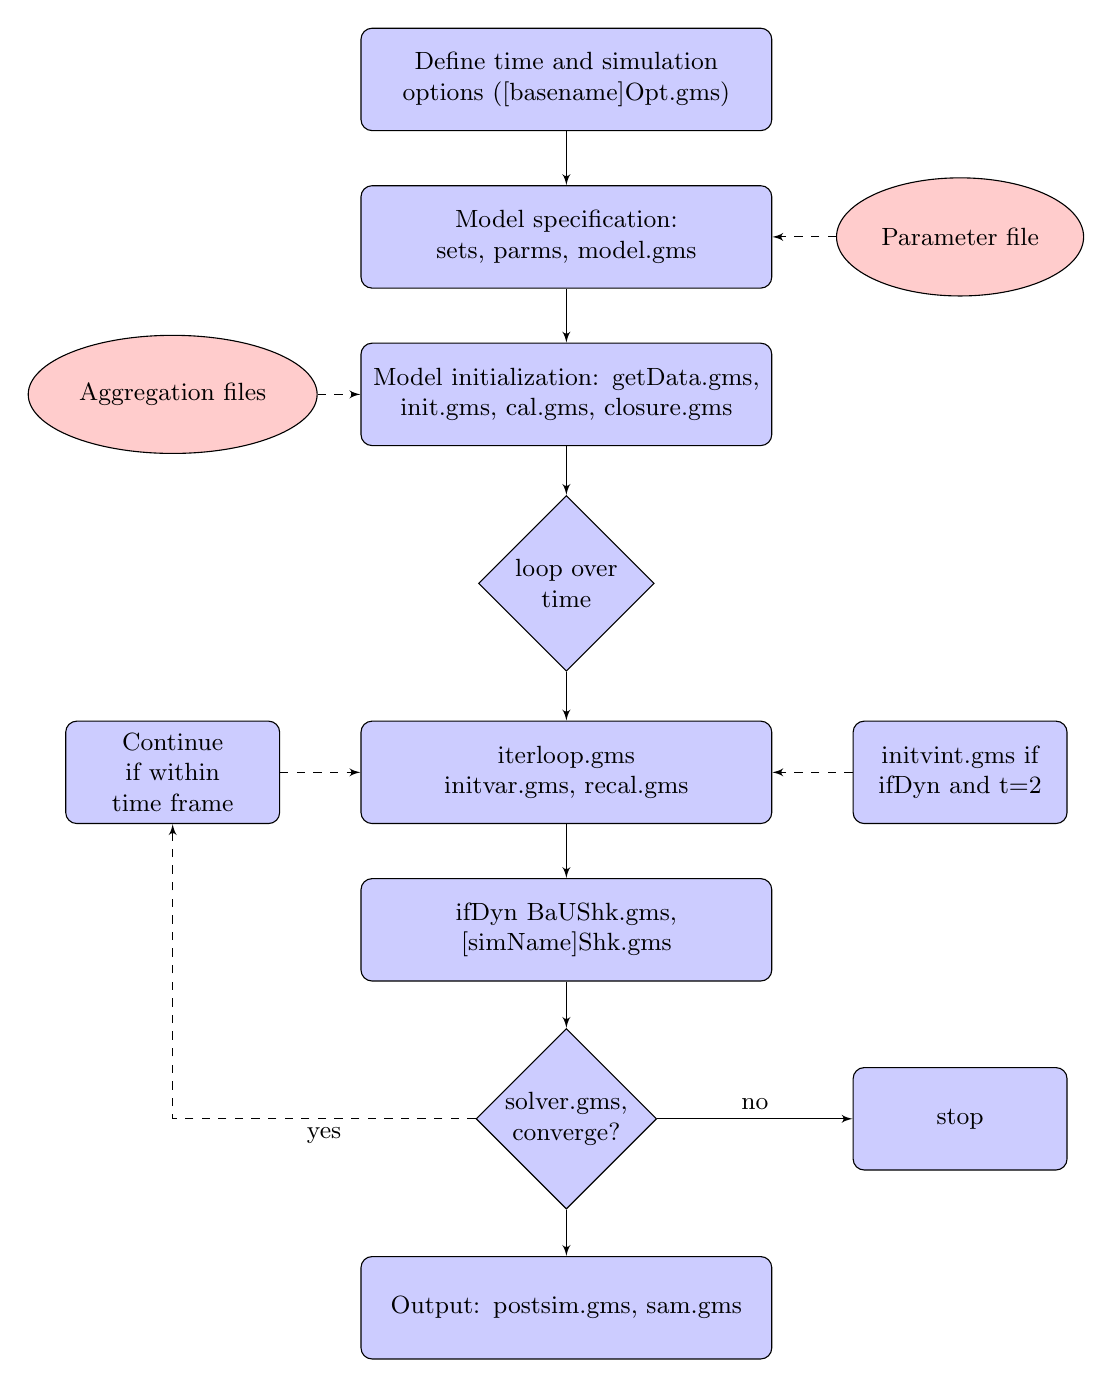
\begin{tikzpicture}[node distance = 2cm, auto]
\small
% Place nodes
\node [block] (init) {Define time and simulation options ([basename]Opt.gms)};
\node [block, below of=init] (modSpec) {Model specification: sets, parms, model.gms};
\node [cloud, right of=modSpec] (prmFile) {Parameter file};
\node [block, below of=modSpec] (modInit) {Model initialization: getData.gms, init.gms, cal.gms, closure.gms};
\node [cloud, left of=modInit] (aggFile) {Aggregation files};
\node [decision, below of=modInit, node distance=2.4cm] (loop) {loop over time};
\node [block, below of=loop, node distance=2.4cm] (iterloop) {iterloop.gms \\ initvar.gms, recal.gms};
\node [block, below of=iterloop] (shocks) {ifDyn BaUShk.gms, [simName]Shk.gms};
\node [smallblock, right of=iterloop, node distance=5cm] (initvint) {initvint.gms if ifDyn and t=2};
\node [decision, below of=shocks, node distance=2.4cm] (solver) {solver.gms, converge?};
\node [smallblock, right of=solver, node distance=5cm] (stop) {stop};
\node [smallblock, left of=iterloop, node distance=5cm] (timecheck) {Continue if within time frame};
\node [block, below of=solver, node distance=2.4cm] (output) {Output: postsim.gms, sam.gms};
% Draw edges
\path [line] (init) -- (modSpec);
\path [line] (modSpec) -- (modInit);
\path [line] (modInit) -- (loop);
\path [line] (loop) -- (iterloop);
\path [line] (iterloop) -- (shocks);
\path [line] (shocks) -- (solver);
%\path [line] (loop) -| node [near start] {yes} (iterloop);
\path [line,dashed] (solver) -| node [near start, color=black] {yes} (timecheck);
\path [line,dashed] (timecheck) -- (iterloop);
\path [line] (solver) -- node {no}(stop);
\path [line] (solver) -- (output);
\path [line,dashed] (aggFile) -- (modInit);
\path [line,dashed] (prmFile) -- (modSpec);
%\path [line,dashed] (prmFile) |- (modInit);
\path [line,dashed] (initvint) -- (iterloop);
\end{tikzpicture}
\end{center}
\end{figure}

In a typical application, the user will create a project directory with the base
name of the project. The simulation files will be contained in that directory.
The distribution comes with several files that provide examples of how to run
both comparative static and dynamic simulations. Beyond the aggregated data
files, the user needs to prepare a file with the model parameters. This file can
be fairly generic if based on an aggregation of one of the existing parameter
files. However, there a number of options that users need to define to complete
the model specification---such as the labor market closure.

\subsubsection{The user-based parameter file}

While most of the inputs to the model are prepared by the aggregation facility,
it is up to the user to prepare the file with project-specific model parameters.
The file has the name \texttt{[basename]Prm.gms}. There is a generic parameter
file that simply initializes all model parameters to those generated by the
aggregation facility. These can be overridden---after the ones from the
aggregation facility are loaded, but before the initialization of the model
parameters. The read-in parameters will have a suffix of '0'. The model
parameters have no suffix.

The aggregated parameters reflect values used by the OECD's Environment
Directorate Env-Linkages Model (\cite{ChateauetalOECD2014}). The
\texttt{Envisage} Model has some new features not fully reflected in the
original Env-Linkages Model, such as the power and water module. The file does
include some initial levels for the power elasticities, but [for the moment]
does not include the elasticities for the water module. These must be entered by
the user if the water module is active. Another critical set of elasticities is
the natural resource supply elasticities. [NEW] It is the user's responsibility
to enter these elasticities (for the original model aggregation). The user must
enter a pair of elasticities for each natural resource and for all regions. The
parameter to be initialized is \texttt{etanrfx0} that takes three indices:
region, activity and a special one that takes the values of 'lo' and 'hi'. This
latter is represented by the set \texttt{lh}. These refer to the supply
elasticity to apply as a function of market conditions. The 'lo' supply
elasticity is to be used for a market under contraction. The 'up' supply
elasticity is to be used for an expanding market. Intuition suggests that the
'lo' elasticity will be greater than the 'hi' elasticity, i.e. it is easier to
contract supply than to expand it. These should be carefully scrutinized and
potentially adjusted during baseline simulation runs.

[NEW] The user must enter the investment allocation elasticities to be used with
the flexible capital flow specification. The initial elasticities are to be
initialized with the parameter \texttt{epsRor0}. The default value for the GTAP
model is 10.

[NEW] There are a number of parameters to be entered by the user for the
USAGE-inspired capital account closure. The user must enter the bounds on the
growth of capital in any given year. These are entered in the parameters
'\texttt{grKMin0}' and '\texttt{grKMax0}'. Normal trend growth is entered in the
parameter '\texttt{grKTrend0}'. The curvature of the logistic function at the
equilibrium point of the capital supply schedule is entered in the parameter
'\texttt{chigrK0}'. The user must also enter the so-called normal rate of
return, from which the deviations are evaluated. This is entered in the
parameter '\texttt{RoRn0}'.

The comparative static version of the model uses a weighted average of the
vintage-dependent elasticities. Users are free to change the weights, where the
default values are 0.8 for \emph{Old} and 0.2 for \emph{New}.

There are a number of other key assumptions that are included in the parameter
file. The first relates to the labor market assumptions. The user must
initialize the matrix of options in the parameter \texttt{labHyp}. It has a
regional and skill index and 11 attributes described below.

\begin{enumerate}
   \item \texttt{omegam}. This determines labor market segmentation. A finite
         value will implement labor market segmentation---typically defined over
         agricultural versus non-agricultural activities. Perfect labor mobility
         is implemented if the value is infinity (\texttt{INF}). If it is
         finite, this will be the value of the labor mobility elasticity in
         equation~(\ref{eq:migr}), $\omega^m$, the elasticity of rural to urban
         migration with respect to the expected urban wage premium.
   \item \texttt{migr0}. This determines the initial level of migration as a
         percent of the rural labor force. For example, if it is set to 1.0,
         the initial level of rural to urban migration will be set to 1\% of the
         rural labor force. It is ignored if the migration elasticity is
         infinity.
   \item \texttt{uezRur0}, \texttt{uezUrb0}. These parameters provide the
         initial unemployment rate (in percent) in respectively the rural and
         urban labor markets. In the case of full labor mobility, only the urban
         unemployment rate is active and the rural rate is ignored.
   \item \texttt{uezminzRur0}, \texttt{uezminzUrb0}. These parameters provide
         the lower bound for the unemployment rate (in percent) in respectively
         the rural and urban labor markets. The rural rate is ignored in the
         case of full labor mobility. An error will be issued if the initial
         unemployment rate is less than the minimum unemployment rate.
   \item \texttt{resWageRur0}, \texttt{resWageUrb0}. These parameters determine
         the initial level of the reservation wage with respect to the
         prevailing wage. A value of 1 indicates that the reservation wage is
         binding and the the unemployment rate is greater than (or equal to) the
         minimum unemployment rate. A value less than one indicates the distance
         between the initial equilibrium wage and the reservation wage. The
         rural reservation wage is ignored in the case of full labor mobility.
         A value of \texttt{NA} indicates full employment (at all times). An
         error will be issued if the value is greater than 1.
   \item \texttt{omegarwg} \texttt{omegarwue} \texttt{omegarwp}. The reservation
         wage is a function of three indicators---the growth of per capita GDP,
         the unemployment rate and the CPI. The elasticity is positive for
         income growth and the CPI. The reservation wage is negatively related
         to the unemployment rate, i.e. an increase in unemployment would tend
         to dampen the reservation wage. To avoid problems with division by
         zero, the relationship between the reservation wage and unemployment is
         converted to a relationship between the reservation wage and the
         employment rate, i.e. $(1-\mathit{UE})$. Thus if the elasticity of the
         reservation wage is $\omega^{\mathit{ue}}$, the elasticity of the
         reservation wage with respect to the employment rate is
         $-\omega^{\mathit{ue}}\left(1 - \mathit{UE}\right)/\mathit{UE}$. The
         user is expected to enter the elasticity with respect to the employment
         rate and it should be a positive number.
\end{enumerate}

There are three additional parameters that allow for control of the dynamics of
the capital market. The first, \texttt{cap\_out\_Ratio0}, allows for overriding
the initial capital to GDP ratio. The initial capital stock is an estimate
derived from the Penn World
Tables.\footnote{\url{http://www.rug.nl/ggdc/productivity/pwt/}} For some
countries and/or regional aggregations the estimates can lead to significant
jumping off problems in the initial years. A value of \texttt{NA} will ignore
the override. The parameter is entered as a multiplicative adjustment
of the initial capital stock. The default value is 1.0.
The second is the depreciation rate, \texttt{deprT}, which for
some rapidly growing countries is too low. The default GTAP value is 4\%. The
third is an investment target, \texttt{invTarget0}. Users can input this for
particular years, e.g. 2030 and 2050. Code in the 'Opt' file will translate
these targets into linear changes for the investment target, for example between
2011 and 2030 and then between 2030 and 2050, in order to smooth the path
between target years.

The final section allows the user to implement 'twists' to the Armington
preference parameters. There are three sets of twist parameters and one
twist-related regional mapping set. The top-level Armington twists require two
different parameters depending on the value of \texttt{ArmFlag}. In the case of
national sourcing, i.e. when \texttt{ArmFlag} = 0, the relevant twist parameter
is \texttt{twt1}, which is region-, commodity and time-specific. With
agent-based sourcing, i.e. when \texttt{ArmFlag} = 1, the relevant twist
parameter is \texttt{tw1}, that is in addition agent-specific. A positive value,
for example 0.02, would lead to a change in the ratio of imports to domestic
demand of 2~percent---assuming constant prices. The parameter \texttt{tw2} is
applied to the second level nesting. The $r$ index refers to the importing
country. The twist can be applied to one single region, or a group of regions.
The user designates the targeted exporters in the regional mapping set
\texttt{rtwtgt}. The first regional index in the mapping set refers to the
targeted exporters and the second regional index refers to the importer. For
example, to increase the import shares of China, Japan and Korea in the U.S.
using the twist, the relevant mapping is \texttt{(chn,jpn,kor).usa}. Note that
in this implementation, the same twist is applied uniformly across the targeted
exporters.

\subsection{Common options}

The first set of global options are entered as definitions through GAMS'
\texttt{\$setGlobal} statement. The following enumerates the options:

\begin{enumerate}
   \item \textbf{wDir}. By default this is set to the active directory.
   \item \textbf{SSPMOD}. This option defines the choice of the economic model
         used for the SSP GDP projections. There are currently two choices:
         \texttt{OECD} and \texttt{IIASA}.\footnote{The PIK projections have not
         been processed since they reflect a fixed aggregation of 32 regions,
         whereas the OECD and IIASA projections were done for most countries.}
   \item \textbf{SSPSCEN}. This option defines which SSP to use for the GDP
         projections (and will be combined with the model choice). There are
         five valid options: \texttt{SSP1}-\texttt{SSP5}.
   \item \textbf{LABSCEN}. This option influences the relative growth of skilled
         versus unskilled labor. If it is set to one of the SSPs, the education
         profiles from the SSPs---with the user mappings of skilled workers to
         education levels (\texttt{educMap}) together with the \texttt{skLabgrwgt}
         parameter (see below)---will
         determine the growth rate of skilled workers. The growth of unskilled
         workers will be determined residually so that the overall growth or
         workers matches the growth of the working age population. If this
         parameter is not equal to one of the SSPs, both skilled and unskilled
         workers will grow at the same rate as the working age population,
         i.e. no differentiation of growth by skill.
   \item \textbf{POPSCEN}. This option defines which population projection to
         use. There are ten valid options. The IIASA SSP population projections
         are labeled \texttt{SSP1}-\texttt{SSP5}. The scenario file also
         includes four UN population projections: \texttt{UNMED2010},
         \texttt{UNMED2012}, \texttt{UNMED2015} and \texttt{UNMED2017}. Finally, the World Bank's
         GIDD projections are available with the label \texttt{GIDD}. The latter
         is intended to duplicate UNMED2015. It is only available through 2050.
   \item \textbf{OVERLAYPOP}. This option allows to replace GTAP's base year
         population level with that from the scenario database. In any case,
         only the growth rates from the population projections are used from the
         initial base year level.\footnote{There is currently an inconsistency
         in the population levels in the SSP database and GTAP. In the former,
         population is in levels and in the latter it is millions.
         The inputs from the SSP database are currently scaled by a million to
         make them consistent with the GTAP units. The population scale factor
         can be used to improve the population scale on an as-need basis.}
   \item \textbf{TASS}. This option determines the specification for the
         aggregate land supply curve. Valid options are: \texttt{KELAS} for
         iso-elastic supply, \texttt{LOGIST} for logistic supply curve,
         \texttt{HYPERB} for hyperbola supply curve, and \texttt{INFTY} for
         infinitely elastic (i.e. horizontal) supply curve.
   \item \textbf{WASS}. This option determines the specification for the
         aggregate water supply curve. It has the same valid options as the
         aggregate land supply curve.
   \item \textbf{utility}. This option determines the specification of the
         household utility function. Five options are available: \texttt{CD} for
         the Cobb-Douglas utility function, \texttt{LES} for the linear
         expenditure system, \texttt{ELES} for the extended linear expenditure
         system, \texttt{AIDADS} for the AIDADS demand system, and \texttt{CDE}
         for the Constant-difference-in-elasticity demand system. The
         \texttt{CD}, \texttt{LES} and \texttt{AIDADS} are new options. The LES
         is calibrated to the Frisch parameter, which is currently
         parameterized in the calibration routine (\texttt{cal.gms}), but it
         would be preferable to have this entered as user input. AIDADS is
         coded, but there is no calibration. It has been tested assuming the LES
         as one of the special cases of AIDADS. The Cobb-Douglas simply uses the
         base year budget shares to calibrate the marginal budget shares and the
         subsistence minima are set to zero.
   \item \textbf{NRITER}. This option controls the number of iterations when
         running the model convergence in single country mode. As this has not
         been tested with the latest version of the model, it is best to set
         this option to 0.
   \item \textbf{savfFlag}. This option controls the capital account closure.
         Three options are currently available. A value of \texttt{capFix} uses
         the fixed capital account closure rule. A value of \texttt{capFlexGTAP}
         uses the flexible capital account closure rule of the GTAP model. This
         closure allocates global savings in order to equalize expected returns
         across regions. A value of \texttt{capRFix} fixes the ratio of savings
         relative to nominal GDP. A value of \texttt{capFlexUSAGE} uses the flexible
         capital account closure rule inspired by the USAGE model. This closure
         allocates global savings as a function in deviations of the regional
         rate of return from the 'normal' rate of return.
   \item \textbf{intRate}. The user sets this option to the desired value for
         the global real interest rate. The default value is 5\% (i.e. 0.05).
         Note that this parameter is currently only used by the USAGE capital
         account closure.
   \item \textbf{costCurve}. Cost curves are used to implement downward trends
         of new technologies (e.g. renewable electricity). These can be
         implemented using either a hyperbolic (\texttt{HYPERB}) or with a logistic
         function (\texttt{LOGIST}).
   \item \textbf{NTM\_MODULE}. This flag takes the value of \texttt{ON} to implement the
   		 non-tariff measure module, or \texttt{OFF} otherwise. It expects
           to read a GDX-based satellite account with the \emph{basename} followed
           by \texttt{NTM}, e.g., \texttt{ANX1NTM.gdx}.
   \item \textbf{MRIO\_MODULE}. This flag takes the value of \texttt{ON} to implement the
   		 MRIO module, or \texttt{OFF} otherwise. It expects
           to read a GDX-based satellite account with the \emph{basename} followed
           by \texttt{MRIO}, e.g., \texttt{ANX1MRIO.gdx}.
   \item \textbf{RD\_MODULE}. This flag takes the value of \texttt{ON} to implement the
   		 R~\&~D module, or \texttt{OFF} otherwise. It expects
           to read a GDX-based satellite account with the \emph{basename} followed
           by \texttt{R\_D}, e.g., \texttt{ANX1R\_D.gdx}. If the file
           does not exist, it will assume that the cost structure is
           identical to the cost structure for government expenditures
           and scale the costs to some percentage of GDP, which will
           be specified in the \texttt{KnowledgeData0} parameter
           of the user parameter file. The R~\&~D expenses will
           be extracted from government expenditures.
   \item \textbf{DEPL\_MODULE}. This flag takes the value of \texttt{ON} to implement the
   		 resource depletion module for coal
            oil and gas resources, or \texttt{OFF} otherwise. It expects
           to read a GDX-based satellite account with the \emph{basename} followed
           by \texttt{DEPL}, e.g., \texttt{ANX1DEPL.gdx}.
   \item \textbf{CLIM\_MODULE}. This flag takes the value of \texttt{ON} to implement the
   		 climate module. The module is initialized from a
         GAMS file, which is calibrated for a specific reference year, for example,
         2014. (For the moment, there is no version available for GTAP V11 with a 2017 reference year.)
   \item \textbf{DAMAGE\_MODULE}. This flag takes the value of \texttt{ON} to implement the
   		climate damage and adaptation module, or \texttt{OFF} otherwise. This is under development.
   \item \textbf{FBS\_MODULE}. This flag takes the value of \texttt{ON} to implement the
   		 nutrition module, or \texttt{OFF} otherwise. It expects
           to read a GDX-based satellite account with the \emph{basename} followed
           by \texttt{FBS}, e.g., \texttt{ANX1FBS.gdx}.
   \item \textbf{ifBKSTP}. This flag takes the value of \texttt{ON} to implement backstops, or \texttt{OFF} otherwise. This is under development.
   \item \textbf{ifDEPR0}. This flag takes the value of \texttt{ON} to run the
   model on a gross investment basis, or \texttt{OFF} to run the
   model on a net investment basis. When set to \texttt{ON}, the incoming \texttt{VDEP} array is set to 0.
   \item \textbf{ifVINT}. This flag takes the value of 1 to run
   dynamic simulations under the vintage capital assumption, or 0 to run dynamic simulations with a single vintage.
\end{enumerate}

The remaining global options are entered as scalars. The first set provide the
context for the model: comparative static and recursive dynamic with or without
dynamic calibration.

\begin{enumerate}
   \item \textbf{ifDyn}. This option takes two values. A value of 0 indicates a
         comparative static model. A value of 1 indicates a dynamic model. In
         the standard package, this will be set automatically when the
         simulation is invoked and the user sets the \texttt{simType} option.
         Valid values are \texttt{CompStat} and \texttt{RcvDyn}.
   \item \textbf{ifCal}. This option takes two values and is only meaningful for
         dynamic scenarios. A value of 0 runs a dynamic scenario with
         pre-calibrated trends (generated by a baseline). A value of 1 runs a
         dynamic calibration scenario where specific dynamic trends are
         calibrated to exogenous indicators such as GDP. This value will be set
         in dynamic variables by setting the \texttt{ifCal} option when invoking
         the simulation.
   \item \textbf{ifVint}. This options takes the value 0 or 1. It is set
         automatically when the simulation is invoked by the user. A value of 1
         implements vintage capital, which is valid only for dynamic
         simulations. It should be set to 0 for comparative static simulations.
\end{enumerate}

The remaining global options are typically invariant across simulations. The
following list enumerates the options.

\begin{enumerate}
   \item \textbf{inScale}. Scale factor for input data. The input SAM is
         typically in millions. A scale of $10^{-6}$ has been found to be a
         useful scaling factor.
   \item \textbf{outScale}. Scale factor for output data. This is typically just
         the inverse of \texttt{inScale}.
   \item \textbf{popScale}. Scale factor for population. Often set to $10^{-6}$,
         though need to check on the population level inconsistencies.
   \item \textbf{lScale}. Scale factor for labor volumes. [Need to verify scale
         in 'wages' database.]
   \item \textbf{eScale}. Scale factor for energy. The energy volumes are in
         million tons of oil equivalent (MTOE). A scale factor of 0.001 is
         typically used.
   \item \textbf{watScale}. Scale factor for water, typically $10^{-12}$ is
         used. [Check units of volume database.]
   \item \textbf{cScale}. Scale factor for emissions, typically 0.001 is used.
         [Check units for emissions.]
   \item \textbf{ifCEQ}. Convert emissions to CEq. Input emissions are in
         \COT{}eq. If this flag is set to 1, the units will be converted to Ceq.
         The climate module [tbd] is based on emissions in Ceq.
   \item \textbf{ArmFlag}. Set to 1 for agent-based Armington. If the flag is
         set to 0, the top level Armington sourcing is done at the aggregate
         level. [This is a new option.]
   \item \textbf{MRIO}. Set to 1 for agent-based second-level Armington, i.e.
   	     to use the MRIO version of the model. [This is a new option.]
   \item \textbf{ifNRG}. Set to 1 to use energy volumes. This will provide a
         volume/price split for energy commodities.
   \item \textbf{ifNRGNest}. Set to 1 for energy nesting. A value of 0 will have
         only a single nested energy nest.
   \item \textbf{ifMCP}. Set to 1 for MCP. A value of 0 will use NLP. The
         objective function is Walras' Law.
   \item \textbf{ifLandCET}. Set to 1 to use CET for land allocation. A value of
         0 will use the additive CET specification.
   \item \textbf{ifSUB}. Set to 1 to substitute out equations. A value of 0 will
         have the full model specification without substitution. This will
         considerably increase the size of the model.
   \item \textbf{IFPOWER}. Set to 1 for power module, which requires the power
         database, else set to 0.
   \item \textbf{IFWATER}. Set to 1 for water module, which requires the water
         database, else set to 0
   \item \textbf{ifAggTrade}. Set to 1 to aggregate trade in SAM. A value of 0
         will have the full bilateral trade matrices output as part of the SAM.
   \item \textbf{skLabgrwgt}. Set to between 0 and 1. This determines the growth
         assumptions for skilled and unskilled labor. The growth of skilled
         labor is driven by the growth of the appropriate education categories.
         The growth of unskilled labor will then be calculated by residual since
         the growth of overall labor will be determined by the growth of the
         working age population (15-64). One can use this parameter to modulate
         this calculation. If the weight is set to 1, then the growth rate of
         skilled labor will match exactly the growth of the corresponding
         education categories, ignoring any resulting impact on the growth of
         unskilled labor. At the other extreme, if the weight is set to 0, the
         growth of both skilled and unskilled will be identical and equal to the
         growth rate of total labor, i.e. the education profiles are fully
         ignored. Users can choose an intermediate value between 0 and 1.
    \item \textbf{EXR}. This is an exchange rate, which defaults to 0. It can be useful to present results in a different currency, e.g., euro, yen, rands, etc., when working on a study for a particular country or region.
\end{enumerate}

\subsection{Comparative static simulations}

In the current setup, there is very little difference between running
comparative static and simulations dynamic simulations. Both the
\texttt{runsim.gms} and \texttt{[basename]Opt.gms} files are coded to run both
types of simulations. One of the key differences between the two is the time
framework. The standard comparative static simulation has three 'time' periods
labeled \texttt{base}, \texttt{check} and \texttt{shock}. The user is free to
modify these in the 'Opt' file. One of the primary purposes of the comparative
static version of the model is to test model initialization, calibration and
homogeneity. It is also extremely useful to test new model specifications or
parameterizations. With a new model version---for example a new aggregation, new
specification or parameterization, it is always recommended practice to do a
full diagnostic check.

A standard diagnostic check is to run the comparative static model with a single
homogeneity shock in the \texttt{shock} time period. The \texttt{base} year is
never run, it is meant to be able to replicate the initial database. The
\texttt{check} simulation replicates \texttt{base} if the initialization and
calibration are working correctly. For this reason, it is important to look at
the largest residual in the listing file (or console). Open the listing file and
do a search for \texttt{LOOPS}. This should take you to the diagnostics for the
first simulation, i.e. the \texttt{check} simulation. Model diagnostics will
appear by scrolling down---for example model size. The key diagnostic is
\texttt{INITIAL POINT STATISTICS}. The maximum of \texttt{F} should be 0 or near
zero. The largest error should reflect more or less the precision of the input
SAM. One may also want to observe the initial Jacobian to see the range of the
minimum and maximum elements. The range should be relatively narrow. A good
maximum should be no larger than \texttt{1.0e003}. A larger number is an
indication of a scaling issue.

A second check of the model is to look at the values for the \texttt{LHS} in the
list code, which stands for the left-hand side. This is controlled by the
\texttt{LIMROW} option. It may default to either 0 or 3. In the case of 0, no
equations will be listed. In the case of 3, up to 3 in any block will be listed.
Setting \texttt{LIMROW} to a higher number will increase the number of equations
printed in a block, for example: \texttt{Options limrow=100 ;}. The equations
listing shows the value of the residual of an equation, i.e. it collects all
endogenous variables on the left-hand side and evaluates the expression and it
collects all additive exogenous variables and parameters on the right-hand side
and evaluates the right-hand side expression. It then displays the value of the
left-hand side that should match the displayed right-hand side. In most cases,
the right-hand side will evaluate to 0, but it does not have to.\footnote{For
example the labor equilibrium condition will have the exogenous supply of labor
on the right-hand side.} If there is a serious initialization/calibration
problem, it may be necessary to increase \texttt{limrow} and visually go through
the equation listings. For a quick inspection, do a search for \texttt{LHS} to
find the first equation in the listing file. Then search for \texttt{****}. The
four asterisks indicate an 'infeasible' solution. Note that in most cases, the
infeasibility is likely to be a very small number---and typically reflects the
accounting precision of the incoming SAM. To avoid nuisance infeasibility, one
can increase the tolerance level by using the \texttt{tolinfrep} attribute of a
model. In the default settings, the infeasibility tolerance has been set to
\texttt{1.0e-005}, and with a well-balanced SAM, this will generally avoid any listed
infeasibilities.

The homogeneity test requires a shock file. The shock file should have the same
name as the simulation. Thus if the simulation is assigned the name
\texttt{COMP}, the user should create the a file named \texttt{COMPShk.gms}.
Listing~\ref{lst:homShock} illustrates one way of implementing the homogeneity
shock. It tests the value of the time period, and then increases the value of
the exogenous {num\'eraire} by 50\%.

\begin{lstlisting}[language=GAMS, caption={Homogeneity shock}, label=lst:homShock]

if(sameas(tsim,"shock"),
   pnum.fx(tsim) = 1.5*pnum.l(tsim) ;
) ;

\end{lstlisting}

It is useful to do a quick check of the diagnostics by loading the output CSV
file into Excel---and most convenient in Excel's pivot tables. The first thing
to look at is the resulting SAM's. All accounts should be perfectly balanced for
each individual region and for each time period. The second diagnostic is to
compare the \texttt{base} values with the \texttt{check} values. They should be
identical to within vary narrow margins. A third check is to compare the
\texttt{check} values with the \texttt{shock} values. All volume variables
should be identical and all value variables and prices should have increased by
the same percentage amount as the {num\'eraire}, for example 50\%.

These are minimal diagnostics, but the user may want to do others---particularly
if there is a change in specification. These would include shocks to taxes, for
example tariffs, shock to factor stocks, productivity shocks, etc.

The distribution comes with an option file for the '10x10' aggregation, as well
as the generic \texttt{runsim.gms} file. The latter is set to handle many
different situations but users may find it useful and/or necessary to make a
copy of it and insert modifications. The distribution also comes with a command
file that is needed to run the file in a Windows console. To run the homogeneity
test, the command line could be the following:

\begin{verbatim}

   runsim Homog Comp CompStat 0

\end{verbatim}

\noindent The first argument will be the simulation name. In comparative static
simulations the second argument is ignored, but must be present. In dynamic
simulations it is the name of the baseline file. The third argument must be
\texttt{CompStat} for comparative static simulations. The fourth argument is
ignored for comparative static simulations, it is used for dynamic simulations.
It is best to set it to zero.

Users will need to modify the \texttt{runsim} command file for their
installations. An example is depicted below.

\begin{verbatim}

   gams runSim --simName=%1 --BauName=%2 --simType=%3 --ifCal=%4 --baseName=10x10
      --odir=v:\Output\EnvLink\10x10 -idir=..\model5n
      -scrdir=v:\Output\EnvLink\10x10 -ps=9999 -pw=150

\end{verbatim}

\noindent The \texttt{runSim} command file expects at least the four arguments as described
above. It is setup for a specific project. In this case it is setup for a
project named '10x10'. The user needs to specify a folder for the output
directory. Use '.' to specify the current directory. It is also required to
specify the model directory. In the example above, the model directory is at the
same level as the simulation directory and named \texttt{model5n}. The remaining
parameters are optional and the user is free to add others.\footnote{Simulation
output can be voluminous depending on the aggregation and the time span of a
simulation. With increasing use of backups and the cloud, it is sometimes useful
to store output on non-critical storage in order to minimize bandwidth problems
and exceeding allowed storage capacity.}

[NEW 01-Dec-2018] The code in the 'Opt' file has been modified somewhat to improve
the handling of starting point for the model simulation. The old code allowed to
start a simulation by reading in a previous baseline using the
\texttt{execute\_loadpoint} option of GAMS. This is handy if you are running shock
simulations starting in a future year relative to the reference year. The new
code allows the user to specify any simulation as a starting point. The
user can identify the starting simulation on the command line with the
\texttt{startName} option. The Windows command file \texttt{runsimR.cmd} shows
an example of how to use an existing comparative static simulation as a starting
point. If there is no additional shock, the model should solve immediately.

\subsection{Dynamic simulations}

Dynamic simulations are in principle only somewhat more complicated than
comparative static simulations---though in practice raise considerably more
problems. There are two key differences. The first is the time dimension. This
is under the discretion of the user. For GTAP V9, the starting year should be
set at 2011. The terminal year and the intermediate years are at full
discretion. The model is setup to handle year step sizes of more than 1 [though
this probably needs additional testing since it hasn't been used in a while].
One potential problem with multi-year time steps could be convergence, though
this has proven to be less of a problem further out when the model has reached
some sort of steady state. The second key difference is the implementation of
the vintage capital formulation. This in principle should be transparent to the
user.

In principle there is nothing to change in the 'Opt' file nor in the
\texttt{runsim.gms} file. There are default statements that are implemented in
the file \texttt{iterloop.gms} that generate the necessary closures for dynamic
simulations---either the baseline, or pre-calibrated scenarios. Users have some
control in shaping the baseline by modifying or adding statements in the
\texttt{BaUShk.gms} file. In the distributed file, there are two adjustments to
the standard baseline. The first can phase out net capital flows between two
years. The second targets the investment to GDP ratio for
some given future year---both the target and the year are provided by the user.
It endogenizes the savings rate in order to achieve the desired investment
ratio.

Other key dynamic assumptions are embedded in the \texttt{initScen.gms} file
that is in the \emph{Model} directory. In particular the default assumptions on
labor productivity wedges (\texttt{glAddShft} and \texttt{glMltShft}),
autonomous yield growth (\texttt{yexo}), autonomous energy efficiency
improvement (\texttt{aeei} and \texttt{aeec}) and improvements in trade
margins (\texttt{tteff}) are included in this file.[We may revisit this looking
ahead as it is not satisfactory to have these assumptions included in the core
model code.]

The mechanics of the baseline are fairly straightforward---shaping the baseline
is not always straightforward. One of the key issues to arise is the growth of
the capital stock. Base year conditions may lead to extreme jumping off
conditions. For example over-investment may lead to sharply declining rates of
return, and under-investment the reverse. The initial growth of the capital
stock will depend on base year investment (and savings) rates, net capital
flows, the initial stock of capital and the depreciation rate. On balance, one
would like to have as a starting point for the baseline relatively steady
returns to capital, unless there is a good reason to expect rates of return to
rise or drop. It may involve adjusting the initial capital stock and rates of
depreciation. It is not possible to change the initial savings ate including the
capital account, but these can be adjusted over time to yield a desired path for
capital accumulation and rates of return. This is one of the purposes for using
a long-run target for the investment to GDP.

To run the baseline simulation, the command line could be the following:

\begin{verbatim}

   runsim BaU BaU RcvDyn 1

\end{verbatim}

The first argument and second arguments are the name of the baseline. In the
case of running the baseline, the second argument is redundant, but necessary.
The third argument is to invoke a dynamic-type scenario. The fourth argument
invokes the code for dynamic calibration. On occasion, the model will fail
to converge to the terminal year and typically this is due to factor prices
going to some extreme---notably zero for capital in the case of investment
exceeding demand for capital. One may have to restrict the simulation to an
intermediate year and assess intermediate results to understand the nature of
the problem. This can be done by restricting the time loop, for example
\texttt{loop(tsim\$(years(tsim) le 2020)}.

Once the user has a satisfactory baseline, dynamic shock simulations can be
implemented. They are associated with a specific shock file with a base name
linked to the simulation name, \texttt{[simName]Shk.gms}, for example
\texttt{[SSP2ccShk.gms]} to run the SSP2 baseline with climate change impacts.
To run a pre-calibrated dynamic scenario, the command line could be the
following:

\begin{verbatim}

   runsim SSP2CC BaU RcvDyn 0

\end{verbatim}

The first argument is the name of the simulation, and \texttt{runSim.gms} will
try and  open and implement a shock file with a filename that incorporates the
simulation name. The second is the name of the baseline file. At a minimum this
is necessary because the shock simulation needs to extract from the baseline
calibrated information from the baseline---notably the labor productivity
parameter and real government expenditures. Both are assumed to be exogenous
in the shock simulations.\footnote{Users can extract other information from
the baseline on an as-need basis.}

[NEW 01-Dec-2018] The code in the 'Opt' file has been modified to allow for
more flexibility in terms of starting from an existing simulation. The old
code only allowed for starting from the baseline simulation. The new code
allows for starting from any simulation (including the baseline). An existing
simulation is not always the best starting point for solving for a given
year, particularly for a future year. The code allows the user to provide a
year until which the simulation starts from an existing simulation or the
solution from a previous period. To test the baseline simulation, for example,
one could re-run the baseline with no shock but using the calibrated variables
from the baseline, for example:

\begin{verbatim}

   runsimrd noShk BaU RcvDyn 0 BaU 2030

\end{verbatim}

\noindent where the command file \texttt{runsimrd.cmd} is used to invoke
GAMS. This says to run a calibrated recursive dynamic scenario using the
calibrated variables from the baseline scenario called BaU. In addition,
use as the starting point the BaU scenario through the year 2030.
If the dynamics is set up correctly, the
model should solve within 1 iteration in each period. In effect, the
\emph{noShock} scenario is similar in concept to the \emph{Check} scenario for
comparative statics. The rule of thumb is that you can use the baseline till the
first year of a shock. In most cases, initializing with the previous period's
result is better once the shock has been implemented as the shock tends to lead
to sharp deviations from the baseline. For example, if a shock starts in the year 2020,
use the baseline values through 2020 as a starting point, then for subsequent
years, the model with initialize values with the solution from the previous
period---not the baseline simulation. The Windows command file \texttt{runAll.cmd}
contains the batch commands to run the baseline and the no-shock scenario
in sequence. Note that it will make a copy of the 'runSim.gms' file for each
of the simulations and thus the list files will have separate names.

\section{Post-simulation processing}

There is some rudimentary post-simulation processing that is still under development. It
involves two steps. The first step is a GAMS file that reads in a solution and produces
a number of model-based indicators and stores them in different CSV cubes. The CSV
cubes can hold results from one or more simulations. These can be loaded into
Excel files, preferably into pivot tables, and/or alternatively they can be loaded
into statistical or graphical packages such as R for automated generation of figures.

\subsection{User inputs}

The user typically prepares two files---a Windows command file, which facilitates
automating the processing of the GDX file(s), and a user-based option file that
is specific to the simulations. The user-based option file is assumed to have
the name 'baseNameTab.gms', where 'baseNameTab' is replaced with the base name
for the set of simulations, for example '10x10'. Listing~\ref{lst:tabOpt} provides
an example of a 'Tab' file. There are a number of global options that first need
to be initialized.

\begin{enumerate}
\item \textbf{xclDir}. This sets the directory for holding the Excel files. N.B. For
the moment it is best to use the full path name as testing with relative paths
has created errors. For example do not use \texttt{".\textbackslash Doc\textbackslash"} or \texttt{"Doc\textbackslash"}.
This seems to be an issue with the use of the VB scripts under Windows.
\item \textbf{inDir}. This sets the directory for the CSV files. Note that this
will be initialized from the command line parameter '\%oDir\%'.
\item \textbf{wDir}. This sets the working directory. It normally defaults to
the directory that was used to invoke the 'makCSV' program.
\item \textbf{simTgt}. The following set of options initialize the fields for
the pivot tables. \texttt{simTgt} should be set to the code for a valid simulation
or scenario, such as \texttt{BaU}.
\item \textbf{regTgt}. \texttt{regTgt} should be set to the code for a valid region
in the model. Refer to the 'Sets' file to see the valid regions for a specific aggregation.
\item \textbf{timeTgt}. \texttt{timeTgt} should be set to a valid reporting year. Typically
this will be the base, or reference, year.
\item \textbf{actTgt}. \texttt{actTgt} should be set to a valid activity, which
can also be referenced in the 'Sets' file.
\end{enumerate}

The user next provides the reporting years. The set \texttt{tr} is a subset of the
full simulation time framework, which can include all solution years. The time
framework also differs between comparative static and dynamic scenarios. The next
option also permits sub-setting the number of activities reported. It defaults to
all activities and activity aggregations. The user also needs to specify a
conversion factor that is used to convert output from 'primary' electricity
activities. 'Primary' electric activities are those that do not rely on
energy inputs such as coal or gas. The latter have a conversion loss typically
assumed to be a factor of 3, i.e. it takes 3 MTOE of coal or gas to produce
1 MTOE of electricity.\footnote{See \url{https://unstats.un.org/unsd/envaccounting/londongroup/meeting13/LG13_12a.pdf.}}
This factor is only valid for the power-enabled version of the model.

The final set of options is for the cubes (i.e. tables) that will be extracted from
the GDX files. The set \texttt{tables} contains the full list of tables that are
available in the \texttt{makTab.gms} file. The user determines which of the
tables to produce by defining the table subset \texttt{ifTab}.

\begin{lstlisting}[language=GAMS, caption={'Tab' file example for creating CSV cubes}, label=lst:tabOpt]

* ------------------------------------------------------------------------------
*
*     Options for creating CSV cubes
*
*     Users typically select years to output and CSV cubes to create
*
* ------------------------------------------------------------------------------

*  Set folder for Excel files

$setGlobal xclDir "v:\env10\10x10\doc\"

*  Options for CreatePivot file

$setGlobal indir     %oDir%
$setGlobal wdir      %system.fp%
$setGlobal modDir    "..\Model"

*  AgMIP cube?
$setGlobal AgMIP No

$setGlobal DEPLFlag  ON
$setGlobal simTgt    BaU
$setGlobal regTgt    EastAsia
$setGlobal timeTgt   2011
$setGlobal actTgt    Agriculture-a

*  Select report years

$iftheni "%simType%" == "compStat"

   set tr(t)  "Reporting years" / base, check, shock / ;
   set trb(t) "Bilateral trade years" / check, shock / ;
   set trm(t) "MRIO years" / check, shock / ;

$elseifi "%simType%" == "RcvDyn"

   set tr(t) "Reporting years" / 2014, 2017, 2020, 2025, 2030 / ;
   set trb(t) "Bilateral trade years" / 2014, 2030 / ;
   set trm(t) "MRIO years" / 2014, 2030 / ;

$endif

*  Select reporting activities (a subset of aga -- activities + aggregate activities

set aggaga(aga) "Activities to report" ;

*  Report all

aggaga(aga) = yes ;

*  Select MRIO reporting commodities

set mrioc(r,i) "Commodities to report" ;
mrioc(r,i) = no ;

scalar elyPrmNrgConv "Primary electric conversion factor" / 3 / ;

set cpiLab / CPIFUD, CPINFD, CPITOT / ;
set mapCPILab(CPINDX,CPILAB) / TOT.cpiFUD, TOT.CPINFD, TOT.CPITOT / ;

set fpagg / nsk, skl, cap, nrs, lnd / ;
set mapfp(fpagg,fp) /
   nsk.nsk
   skl.skl
   cap.cap
   nrs.nrs
   lnd.lnd
/ ;

*  Pivot tables to create

*  List of tables

set tables /
   gdppop      "Macro data"
   factp       "Factor prices"
   kappah      "Household direct tax rate"
   rgovshr     "Government expenditures"
   savinv      "Savings investment balance"
   xp          "Output by activity"
   va          "Value added by activity and factor"
   inv         "Investment"
   emi         "Emissions"
   cost        "Production costs"
   ydecomp     "Growth decomposition"
   trade       "Trade by sector"
   fdem        "Final demand"
   bilat       "Bilateral trade"
   lab         "Labor demand"
   pow         "Power module"
   sam         "SAM module"
   MRIO        "MRIO table"
   tot         "Terms of trade module"
   nrg         "Energy module"
   depl        "Depletion variables"
   climate     "Climate module"
   shock       "For future use"
   demand      "Demand"
   fbs         "Nutrition module"
   AgMIP       "Cube for AgMIP submission"
/ ;

*  Selected tables

set ifTab(tables) /
   gdppop      "Macro data"
   emi         "Emissions"
   sam         "SAM module"
*  MRIO        "MRIO table"
*  climate     "Climate module"
*  factp       "Factor prices"
*  kappah      "Household direct tax rate"
*  rgovshr     "Government expenditures"
*  savinv      "Savings investment balance"
*  xp          "Output by activity"
*  va          "Value added by activity and factor"
*  inv         "Investment"
*  cost        "Production costs"
*  ydecomp     "Growth decomposition"
*  tot         "Terms of trade"
*  trade       "Trade by sector"
*  fdem        "Final demand"
*  bilat       "Bilateral trade"
*  lab         "Labor demand"
   pow         "Power sector variables"
   nrg         "Energy module"
*  depl        "Depletion variables"
*  shock       "For future use"
   fbs         "Nutrition module"
*  AgMIP       "Cube for AgMIP submission"
/ ;

\end{lstlisting}

\subsection{Extracting the indicators}

The user can invoke the \texttt{makCSV} GAMS program by entering the following
command (or equivalent in the GAMS IDE):

\begin{verbatim}

   gams makCSV --simname=BaU --BaUName=BaU --simType=RcvDyn --ifCal=1
      --ifAppend=0 --BaseName=10x10 --odir=z:\Output\Env10\10x10 -idir=..\Model

\end{verbatim}

Many of the command line options are identical to the \texttt{runsim} command. The user
specifies the name of the simulation (\texttt{simname}), the name of the baseline
simulation, potentially the same (\texttt{BaUname})\footnote{The baseline is on occasion
used to calculate indicators relative to the baseline.}, the simulation type (\texttt{simType}),
and the dynamic calibration flag (\texttt{ifCal}). One of the key command line
arguments is \texttt{ifAppend}. If \texttt{ifAppend} is set to 0, all CSV cubes will be
created anew---erasing any existing CSV cubes. If \texttt{ifAppend} is set to 1, the list
of indicators being extracted will be appended to the end of an existing CSV file---thus
enabling the concatenation of indicators from multiple scenarios in a single cube. If
running from a Windows command file---the first invocation of \texttt{makCSV} should
set the append parameter to 0, and all subsequent invocations should set the append
parameter to 1. The output directory should be where the GDX files are located and will
also be the location of the output CSV files.

Once the CSV cubes have been created, a new command file will also have
been created the contains the commands to convert the CSV cubes into Excel files,
or, if the Excel files already exist, will 'refresh' the pivot tables contained
in the Excel file. This command file will only work in a Windows-based terminal
window as the commands rely on VB scripts. To invoke the command, simply
type 'baseNamePivot', for example '10x10Pivot'. The command file will have been created by the
'makCSV' program. It will only invoke the appropriate commands for the requested
tables. Sample 'runtab.cmd' files will automatically invoke the command.

The whole system relies on four GAMS files and one 'VBS' file that are typically located in the
'Model' directory. The five files are:

\begin{enumerate}
\item \textbf{makCSV}. \texttt{makCSV.gms} is the master GAMS file that reads the options, invokes the
indicator extraction file (makTab) and creates the 'baseNamePivotPivot.cmd' file.
\item \textbf{makTab}. \texttt{makTAB.gms} is the core GAMS file that will extract the
data from GDX files, create indicators, and save them to the CSV files.
\item \textbf{setupPivot}. \texttt{setupPivot.gms} is invoked by the \texttt{makCSV.gms} to
create the command lines for the 'baseNamePivot.cmd' file. It is a small file
invoked using 'batinclude' with arguments that simplifies the creation of the command file.
\item \textbf{CreatePivot}. \texttt{createPivot.gms} writes the VB script that creates
the Excel files with the built-in pivot tables. It is only invoked for Excel files
that are being created for the first time. Otherwise, the 'refresh' VB script is invoked.
\item \textbf{refresh}. \texttt{refresh.vbs} is a VB script that refreshes a
pivot table in an Excel file (without opening Excel).
\end{enumerate}

\subsection{Standard indicators}

The GAMS file 'makCSV.gms' is the file that contains code to create indicators from
simulation results. It extracts selected model results from a simulation (stored as a
GDX container), creates an indicator (potentially without transformation) and in
most cases will also aggregate across user-defined regions and sectors. Classes of
indicators are stored together in CSV cubes. There are several advantages to
having indicators in separate cubes. First, it keeps the sizes of the CSV files
to a reasonable size; making them easier and quicker to load. Second, the
geometry of the cube can be tailored to specific indicators. For example, macroeconomic
indicators typically do not need sector or other qualifiers. Table~\ref{tab:CSVCubes} describes
the current list of CSV cubes.

The following sections describe each of the indicators. The left-hand side
should be thought of as being indexed by aggregate region ($R$), time and simulation.
Normally each modeled region is mapped to its own aggregate region, but could also
be mapped to a true aggregate region that would be composed of 1 or more modeled regions.
The right-hand side is normally composed of a model indicator. There is often a one-to-one
mapping, i.e. the aggregation is just a simple sum of a model indicator.

\subsubsection{The GDPPop cube}

The formulas below calculate the indicators contained in the \texttt{GDPPop} cube. The
formulas need little explanation. GDP at 2005 PPP exchange rates uses the base year
PPP exchange rate derived from the SSP scenario file. The first two population indicators, \texttt{P1564}
and \texttt{PopT}, refer to the exogenous information that is used as input for
a model simulation. The indicator \texttt{Pop} refers to the population that
emerges from the model. This could differ from \texttt{PopT} depending on the
initial level of the population---though the growth rates should be identical.

\[
\mathit{RGDPMP}_R = \sum_{r \in R} {\mathit{RGDPMP}_r}
\]

\[
\mathit{RGDPMPPPP}_R = \sum_{r \in R} {\mathit{RGDPMP}_r \mathit{PPP}}
=\sum_{r \in R} {\mathit{RGDPMP}_r
	\frac{\mathit{GDPScen}_{\mathit{Mod},\mathit{SSP},\mathit{GDPPPP05},r,t0}}{\mathit{GDPScen}_{\mathit{Mod},\mathit{SSP},\mathit{GDP},r,t0}} }
\]

\[
\mathit{GDPMP}_R = \sum_{r \in R} {\mathit{GDPMP}_r}
\]

\[
\mathit{PGDPMP}_R = \sum_{r \in R} {\mathit{GDPMP}_r} \bigg/ \sum_{r \in R} {\mathit{RGDPMP}_r}
\]

\[
\mathit{P1564}_R = \sum_{r \in R} {\mathit{PopT}_{r,\mathit{P1564}}}
\]

\[
\mathit{PopT}_R = \sum_{r \in R} {\mathit{PopT}_{r,\mathit{PTOTL}}}
\]

\[
\mathit{Pop}_R = \sum_{r \in R} {\mathit{Pop}_{r}}
\]

\[
\mathit{RGDPPC}_R = \sum_{r \in R} {\mathit{RGDPMP}_r} \bigg/ \sum_{r \in R} {\mathit{Pop}_{r}}
\]

The GDP cube also contains some indicators of welfare.
The indicators $\mathit{EV}$, $\mathit{EVG}$ and $\mathit{EVI}$
represent the equivalent variation for households, government and
investment expenditures, respectively. The household welfare indicator
is derived from the indirect utility function for the user-chosen
utility function. Government and investment expenditure functions have
a simple formula for equivalent variation based on the CES preference function.
Note that the model
allows for multiple households, though the standard GTAP database only
includes a single representative household.
The remaining three indicators measure the volume of private,
public and investment expenditures.

\[
\mathit{EV}_R = \sum_{r \in R} \sum_{h} {\mathit{EV}_{r,h}}
\]

\[
\mathit{EVG}_R = \sum_{r \in R} {\mathit{YFD}_{r,\mathit{gov}}
	\frac{\mathit{YFD}_{r,\mathit{gov},t0}}{\mathit{YFD}_{r,\mathit{gov}}}}
\]

\[
\mathit{EVI}_R = \sum_{r \in R} {\mathit{YFD}_{r,\mathit{inv}}
	\frac{\mathit{YFD}_{r,\mathit{inv},t0}}{\mathit{YFD}_{r,\mathit{inv}}}}
\]

\[
\mathit{EVT}_R = \mathit{EV}_R + \mathit{EVG}_R + \mathit{EVI}_R
\]

\[
\mathit{XFD}_R = \sum_{r \in R} \sum_h {\mathit{XFD}_{r,\mathit{h}}}
\]

\[
\mathit{XFDG}_R = \sum_{r \in R} {\mathit{XFD}_{r,\mathit{gov}}}
\]

\[
\mathit{XFDI}_R = \sum_{r \in R} {\mathit{XFD}_{r,\mathit{inv}}}
\]

\subsubsection{The FactP cube}

The \texttt{FactP} cube provides aggregate (or economy-wide) factor prices. The labels
for capital, land and water return are hard-coded. The labels for the aggregate
wages will be the same as the labels for the labor types (e.g. \texttt{nsk} and \texttt{skl}).

\[
\mathit{AW}_{R,l} = \sum_{r \in R} {\sum_a{\mathit{PF}_{r,l,a}\mathit{XF}_{r,l,a}}} \bigg/ \sum_{r \in R} {\sum_a{\mathit{XF}_{r,l,a}}}
\]

\[
\mathit{TRENT}_{R} = \sum_{r \in R} {\sum_a{\mathit{PF}_{r,\mathit{cap},a}\mathit{XF}_{r,\mathit{cap},a}}} \bigg/ \sum_{r \in R} {\sum_a{\mathit{XF}_{r,\mathit{cap},a}}}
\]

\[
\mathit{PTLand}_{R} = \sum_{r \in R} {{\mathit{PTLand}_{r} \mathit{TLand}_{r}}} \bigg/ \sum_{r \in R} {\mathit{TLand}_{r}}
\]

\[
\mathit{PTNRS}_{R} = \sum_{r \in R} {\sum_a{\mathit{PF}_{r,\mathit{nrs},a}\mathit{XF}_{r,\mathit{nrs},a}}} \bigg/ \sum_{r \in R} {\sum_a{\mathit{XF}_{r,\mathit{nrs},a}}}
\]

\[
\mathit{PTH2O}_{R} = \sum_{r \in R} {\sum_a{\mathit{PF}_{r,\mathit{wat},a}\mathit{XF}_{r,\mathit{wat},a}}} \bigg/ \sum_{r \in R} {\sum_a{\mathit{XF}_{r,\mathit{wat},a}}}
\]

\subsubsection{The Kappah cube}

This cube contains only the average rate of transfer between households and
government.\footnote{The main purpose of this is to assess the impacts of the
standard closure rule that has the government deficit fixed and net household
transfers adjust to meet the fiscal target.}

\[
\mathit{Kappah}_{R} = \sum_{r \in R} {\kappa^h_r \mathit{YH}_{r}} \bigg/ \sum_{r \in R} {\mathit{YH}_{r}}
\]

\subsubsection{The RGovShr cube}

This cube contains only the average ratio of real
government expenditure to real GDP.\footnote{In the standard baseline, this
ratio is fixed and drives the growth of real government expenditures.
In shock simulations, the ratio is endogenous and real government
expenditures are fixed to baseline levels.}

\[
\mathit{RGovShr}_{R} = 100 \cdot \sum_{r \in R} {\mathit{XFD}_{r,\mathit{gov}}} \bigg/ \sum_{r \in R} {\mathit{RGDPMP}_{r}}
\]

\clearpage

\begin{table}[H]
\caption{CSV cubes}
\label{tab:CSVCubes}
\begin{center}
\small
\rowcolors{2}{TableOdd}{TableEven}
\rowcolors{1}{}{lightblue}
\begin{tabular}{p{2.0cm} p{13.0cm}}
\arrayrulecolor{TableBorder}\specialrule{1pt}{0pt}{0pt}
{\normalsize \textbf{\emph{File name}}} & {\normalsize \textbf{\emph{Description}}} \\
\arrayrulecolor{TableBorder}\specialrule{1pt}{0pt}{0pt}
GDPPop & Contains GDP and population including: real GDP at market price (\texttt{rgdpmp}),
nominal GDP at market price (\texttt{gdpmp}),
GDP at market price deflator (\texttt{pgdpmp}),
working age population (\texttt{P1564}),
input population (\texttt{PopT}),
simulated population (\texttt{Pop}), and
real GDP per capital (\texttt{rgdppc}). \\
Factp & Contains aggregate factor prices including: wages identified by skill,
capital (\texttt{trent}), land (\texttt{ptland}), natural resources (\texttt{ptnrs}) and water, if available (\texttt{pth2o}). \\
kappah & Contains net direct transfers to housholds as a share of income (\texttt{kappah}). \\
RGovShr & Contains real government expenditures as a share of real GDP (\texttt{rgovshr}). \\
savinv & Contains various indicators relating to savings and investment including: nominal GDP at market price (\texttt{gdpmp}),
real GDP at market price (\texttt{rgdpmp}),
real investment as a share of real GDP (\texttt{rinvshr}),
aggregate real investment (\texttt{rinv}),
aggregate nominal investment (\texttt{inv}),
aggregate nominal household saving (\texttt{savh}),
household savings rate (\texttt{aps}),
nominal government saving (\texttt{savg}),
nominal foreign saving (\texttt{savf}) and
nominal depreciation (\texttt{deprY}). \\
Output & Contains various indicators relating to output: unweighted output (\texttt{xp}),
output weighted by base year prices (\texttt{xpw}),
nominal output (\texttt{xpd}),
output price using unweighted volumes (\texttt{px}),
output price using base year price-weighted volumes (\texttt{pxn}),
GAPS unweighted volume (\texttt{xpg\_GAPS}), and
Envisage output using GAPS base year volume (\texttt{xpg\_Env}). \\
VA & Contains various indicators relating to value added by activity and factor: nominal value added (\texttt{va\_d}),
value added weighted by base year prices (\texttt{va\_n}),
price of value added using base-year price-weighted volumes (\texttt{pva\_n}),
unweighted volumes (\texttt{va}), and
price of value added using unweighted volumes (\texttt{pva}). \\
INV & Contains various indicators relating to investment by sector: volume of sectoral investment (\texttt{inv\_sec}),
nominal investment by sector (\texttt{invd\_sec}),
sectoral share of aggregate nominal investment (\texttt{invd\_shr}),
sectoral share of nominal value added (\texttt{va\_shr}), and
ratio of sectoral investment share and value added share (\texttt{invRatio}). \\
EMI & Contains various indicators relating to greenhouse gas emissions: total emissions (\texttt{emi}),
emissions linked to intermediate and final demand (\texttt{emi\_io}),
emissions linked to factor use (\texttt{emi\_fp}), and
emissions linked to output (\texttt{emi\_xp}). \\
Cost & Contains various indicators relating to decomposing production cost: change in production cost (\texttt{delpx}),
change in output (\texttt{delxp}),
contribution of change in cost arising from change in input price (\texttt{pcshr}),
contribution of change in cost arising from change in technology mix (\texttt{xcshr}), and
cost share of input (\texttt{cshr}). \\
YDecomp & Contains various indicators relating to decomposing GDP growth: nominal GDP at
factor cost (\texttt{gdpfc}),
real GDP at factor cost (\texttt{rgdpfc}),
real GDP at factor cost deflator (\texttt{pgdpfc}),
contribution of GDP growth from factor growth (\texttt{qdel}), and
contribution of GDP growth from factor productivity  (\texttt{ldel}). \\
Trade & Contains various indicators relating to trade: nominal exports (\texttt{exp\_d}),
real exports (\texttt{exp}),
export tax rate (\texttt{etax}),
nominal imports at FOB prices (\texttt{imp\_fob\_d}),
real imports at FOB prices (\texttt{imp\_fob}),
nominal imports at CIF prices (\texttt{imp\_cif\_d}),
real imports at CIF prices (\texttt{imp\_cif})
import tariff (\texttt{mtax}) and
domestic absorption  (\texttt{Absorb}). \\
Lab & Contains various indicators relating to labor markets: labor supply (\texttt{ls}),
wage (\texttt{twage}),
real wage (\texttt{trwage}),
rural to urban migration (\texttt{migr}),
labor supply by zone (\texttt{lsz}),
average wage by zone (\texttt{awage}),
equilibrium wage by zone (\texttt{ewage})
average real wage (\texttt{arwage}) and
average equibrium wage  (\texttt{aewage}). \\
Power & Contains various indicators relating to power: output (\texttt{XP}), and
average cost (\texttt{PX}). \\
\arrayrulecolor{TableBorder}\specialrule{1pt}{0pt}{0pt}
\end{tabular}
\end{center}
\end{table}

\subsubsection{The SavInv cube}

The \texttt{SavInv} cube contains the indicators below. Note that
investment should equal aggregate savings (household, government and foreign)
plus depreciation for any regional aggregation. Moreover, the sum of
foreign saving at the world level should equal 0.

\[
\mathit{RGDPMP}_R = \sum_{r \in R} {\mathit{RGDPMP}_r}
\]

\[
\mathit{GDPMP}_R = \sum_{r \in R} {\mathit{GDPMP}_r}
\]

\[
\mathit{RInvShr}_{R} = 100 \cdot \sum_{r \in R} {\mathit{XFD}_{r,\mathit{inv}}} \bigg/ \sum_{r \in R} {\mathit{RGDPMP}_{r}}
\]

\[
\mathit{RInv}_{R} = \sum_{r \in R} {\mathit{XFD}_{r,\mathit{inv}}}
\]

\[
\mathit{Inv}_{R} = \sum_{r \in R} {\mathit{YFD}_{r,\mathit{inv}}}
\]

\[
\mathit{SavH}_{R} = \sum_{r \in R} {\mathit{S}^h_{r}}
\]

\[
\mathit{SavG}_{R} = \sum_{r \in R} {\mathit{S}^g_{r}}
\]

\[
\mathit{SavF}_{R} = \sum_{r \in R} {\mathit{PW}^{\mathit{sav}}\mathit{S}^f_{r}}
\]

\[
\mathit{DeprY}_{R} = \sum_{r \in R} {\mathit{DeprY}_{r}}
\]

\[
\mathit{APS}_{R} = 100 \cdot \sum_{r \in R} {\mathit{S}^h_{r}}  \bigg/ \sum_{r \in R} {\mathit{YD}_{r}}
\]

\subsubsection{The Output cube}
The output cube contains various indicators related to output. Three
reflect different measures of the level of output---nominal (\texttt{XPD}),
unweighted real (\texttt{XP}) and weighted real (\texttt{XPW}).
For most purposes the appropriate index is the weighted real---particularly
when aggregating across activities using different units. Potential
exceptions are when aggregating energy indicators as these may be
evaluated in the same units, for example MTOE or GWhr.
Similarly there
are two price indices: unweighted (\texttt{PX}) and weighted  (\texttt{PXN}).
The cube also contains the total factor productivity parameter (for installed
or \emph{Old} capital).

\[
\mathit{XP}_{R,A} =
\sum_{r \in R} {\sum_{a \in A} {\mathit{XP}_{r,a}}}
\]

\[
\mathit{XPW}_{R,A} =
\sum_{r \in R} {\sum_{a \in A} {\mathit{PX}_{r,a,0}\mathit{XP}_{r,a}}}
\]

\[
\mathit{XPD}_{R,A} =
\sum_{r \in R} {\sum_{a \in A} {\mathit{PX}_{r,a}\mathit{XP}_{r,a}}}
\]

\[
\mathit{PX}_{R,A} =
\sum_{r \in R} {\sum_{a \in A} {\mathit{PX}_{r,a}\mathit{XP}_{r,a}}}
\bigg/
\sum_{r \in R} {\sum_{a \in A} {\mathit{XP}_{r,a}}}
\]

\[
\mathit{PXN}_{R,A} =
\sum_{r \in R} {\sum_{a \in A} {\mathit{PX}_{r,a}\mathit{XP}_{r,a,0}}}
\bigg/
\sum_{r \in R} {\sum_{a \in A} {\mathit{PX}_{r,a,0} \mathit{XP}_{r,a,0}}}
\]

\[
\mathit{lambdaxpOld}_{R,A} =
\sum_{r \in R} {\sum_{a \in A}
{\lambda^{\mathit{xp}}_{r, a, \mathit{Old}} \mathit{PXv}_{r,a, \mathit{Old},0}\mathit{XPv}_{r,a, \mathit{Old}}}}
\bigg/
\sum_{r \in R} {\mathit{PXv}_{r,a, \mathit{Old},0}\mathit{XPv}_{r,a, \mathit{Old}}}
\]

\noindent [Optional] There are two additional volume indicators linked
to an external estimate of base year volumes.\footnote{This is particularly
useful where the external estimate of base year volumes is in recognizable
units---such as tons, joules, etc.} The first indicator is the external
indicator itself---in its own units and with its own growth trends (e.g. from
an FAO or IEA projection). The second is the growth trend using the Envisage
results but re-based to that of the external data. This allows for easier
comparison of trends between institutions. In the case of the comparison
with the FAO GAPS projections, the FAO projections are labeled \texttt{xpg\_GAPS}
and the Envisage projections are labeled \texttt{xpg\_Env}. Note that the base
years for GAPS and Envisage do not line up (2012 versus 2011), nor do the time
steps line up.

\subsubsection{The VA cube}
The value added cube contains various indicators related to value added. In addition
to the various endowments that are part of the model definition, the indicators
also include aggregations for labor (\texttt{tlab}), all non-labor factors (\texttt{tcap}) and all factors (\texttt{tot}). In most cases, the
$\mathit{VA\_N}$ indicator is the most appropriate for assessing
aggregate value added. The $\mathit{VA}$ indicator can be
used in some cases to evaluate labor in person years
depending on the calibration choices of the user.

\[
\mathit{VA\_D}_{R,A,V} =
\sum_{r \in R} {\sum_{a \in A} {\sum_{f \in V} {\mathit{PF}_{r,f,a}\mathit{XF}_{r,f,a}}}}
\]

\[
\mathit{VA\_N}_{R,A,V} =
\sum_{r \in R} {\sum_{a \in A} {\sum_{f \in V} {\mathit{PF}_{r,f,a,0}\mathit{XF}_{r,f,a}}}}
\]

\[
\mathit{PVA\_N}_{R,A,V} =
\sum_{r \in R} {\sum_{a \in A} {\sum_{f \in V} {\mathit{PF}_{r,f,a}\mathit{XF}_{r,f,a}}}}
\bigg/
\sum_{r \in R} {\sum_{a \in A} {\sum_{f \in V} {\mathit{PF}_{r,f,a,0}\mathit{XF}_{r,f,a}}}}
\]

\[
\mathit{VA}_{R,A,V} =
\sum_{r \in R} {\sum_{a \in A} {\sum_{f \in V} {\mathit{XF}_{r,f,a}}}}
\]

\[
\mathit{PVA}_{R,A,V} =
\sum_{r \in R} {\sum_{a \in A} {\sum_{f \in V} {\mathit{PF}_{r,f,a}\mathit{XF}_{r,f,a}}}}
\bigg/
\sum_{r \in R} {\sum_{a \in A} {\sum_{f \in V} {\mathit{XF}_{r,f,a}}}}
\]

\subsubsection{The INV cube}
The investment cube contains investment by sector---both in volume
and value terms. The formulas take into account multi-year step sizes.
The \texttt{InvRatio} indicator measures an activity's share of investment
relative to its share of value added (in nominal terms).

\[
\mathit{INV\_SEC}_{R,A} =
\sum_{r \in R} {\sum_{a \in A} {
\frac{\delta_{r,t-n}}{1-\left(1-\delta_{r,t-n}\right)^n}\left[
\sum_v{K^v_{r,a,v,t}} - \left(1-\delta_{r,t-n}\right)^n\sum_v{K^v_{r,a,v,t-n}}\right]
\frac{1}{\chi^k_r}
}}
\]

\[
\mathit{INVD\_SEC}_{R,A} =
\sum_{r \in R} {\sum_{a \in A} {
\frac{\delta_{r,t-n}}{1-\left(1-\delta_{r,t-n}\right)^n}\left[
\sum_v{K^v_{r,a,v,t}} - \left(1-\delta_{r,t-n}\right)^n\sum_v{K^v_{r,a,v,t-n}}\right]
\frac{\mathit{PFD}_{r,\mathit{inv},t-n}} {\chi^k_r}
}}
\]

\[
\mathit{INVD\_SHR}_{R,A} = \frac{
\sum_{r \in R} {\sum_{a \in A} {
\frac{\delta_{r,t-n}}{1-\left(1-\delta_{r,t-n}\right)^n}\left[
\sum_v{K^v_{r,a,v,t}} - \left(1-\delta_{r,t-n}\right)^n\sum_v{K^v_{r,a,v,t-n}}\right]
\frac{\mathit{PFD}_{r,\mathit{inv},t-n}} {\chi^k_r}
}}}
{
\sum_{r \in R} {\sum_{a} {
\frac{\delta_{r,t-n}}{1-\left(1-\delta_{r,t-n}\right)^n}\left[
\sum_v{K^v_{r,a,v,t}} - \left(1-\delta_{r,t-n}\right)^n\sum_v{K^v_{r,a,v,t-n}}\right]
\frac{\mathit{PFD}_{r,\mathit{inv},t-n}} {\chi^k_r}
}}}
\]

\[
\mathit{VA\_SHR}_{R,A} = \frac{
\sum_{r \in R} {\sum_{a \in A} {\sum_f{\mathit{PF}_{r,f,a}\mathit{XF}_{r,f,a}}}}}
{
\sum_{r \in R} {\sum_{a} {\sum_f{\mathit{PF}_{r,f,a}\mathit{XF}_{r,f,a}}}}}
\]

\[
\mathit{InvRatio}_{R,A} = \frac{\mathit{INVD\_SHR}_{R,A}}
{\mathit{VA\_SHR}_{R,A}}
\]

\subsubsection{The Emissions cube}

The emissions cube contains 5 indicators:
total emissions, emissions linked to consumption
of intermediate and final demand, emissions
linked to factor-use and emissions linked to
output. Emission indicators are output for all types of emissions. Physical emissions are all
denominated in unit of gigatons.\footnote{Base
non-greenhouse gas emissions are in units
of gigagrams. They are divided by 1000 to
convert to gigatons.}
Greenhouse gases are also output in units
of CEq and CO2eq. If the model uses units
of CEq, CO2eq is calculated by multiplying
the emission level by a factor of 44/12. In
the contrary case, emissions are converted to
CEq using the factor 12/44.


\[
\mathit{Emi}_{R,\mathit{Tot},\mathit{em}}
= \sum_{r \in R} {\mathit{EmiTot}_{r,\mathit{em}}}
\]

\[
\mathit{Emi\_io}_{R,\mathit{A},\mathit{em}}
= \sum_{r \in R} {\sum_{a \in A} {\sum_i {\mathit{Emi}_{r,\mathit{em},i,a}}}}
\]

\[
\mathit{Emi\_io}_{R,\mathit{fd},\mathit{em}}
= \sum_{r \in R} { {\sum_i {\mathit{Emi}_{r,\mathit{em},i,\mathit{fd}}}}}
\]

\[
\mathit{Emi\_fp}_{R,\mathit{A},\mathit{em}}
= \sum_{r \in R} {\sum_{a \in A} {\sum_{\mathit{fp}} {\mathit{Emi}_{r,\mathit{em},\mathit{fp},a}}}}
\]

\[
\mathit{Emi\_xp}_{R,\mathit{A},\mathit{em}}
= \sum_{r \in R} {\sum_{a \in A}  {\mathit{Emi}_{r,\mathit{em},\mathit{Tot},a}}}
\]

\subsubsection{The Trade cube}

The first set of equations relate to exports.
These are aggregated over regions and commodities,
where the index $I$ is an aggregate commodity,
which may be an individually modeled commodity.
The first two measure aggregate exports
by commodity $I$ at current FOB prices and
at constant FOB prices. The third formula
measures the export tax.

\[
\mathit{EXP\_D}_{R,I} =
\sum_{s \in R} {\sum_{i \in I} {
\sum_d
{\mathit{PWE}_{s,i,d} \mathit{XW}_{s,i,d}}
}}
\]

\[
\mathit{EXP}_{R,I} =
\sum_{s \in R} {\sum_{i \in I} {
		\sum_d
		{\mathit{PWE}_{s,i,d,0} \mathit{XW}_{s,i,d}}
}}
\]

\[
\mathit{ETAX}_{R,I} =
100 \cdot \sum_{s \in R} {\sum_{i \in I} {
		\sum_d
		{\mathit{PWE}_{s,i,d} \mathit{XW}_{s,i,d}}
}} \bigg/
\sum_{s \in R} {\sum_{i \in I} {
		\sum_d
		{\mathit{PE}_{s,i,d} \mathit{XW}_{s,i,d}}
}} - 100
\]

The next set of five equations relate to
imports. The first two equations evaluate current
and constant imports at FOB prices, i.e. these indicators
ignore the trade and transport margins.
The next two equations use CIF import prices.
The final equation evaluates the import tariff
in percentage terms.
Note that the variable $\mathit{XW}$ represents
the supply of exports and is adjusted
by the iceberg parameter to convert to demand
for imports.

\[
\mathit{IMP\_FOB\_D}_{R,I} =
\sum_{d \in R} {\sum_{i \in I} {
		\sum_s
		{\mathit{PWE}_{s,i,d} \lambda^w_{s,i,d} \mathit{XW}_{s,i,d}}
}}
\]

\[
\mathit{IMP\_FOB}_{R,I} =
\sum_{d \in R} {\sum_{i \in I} {
		\sum_s
		{\mathit{PWE}_{s,i,d,0} \lambda^w_{s,i,d} \mathit{XW}_{s,i,d}}
}}
\]

\[
\mathit{IMP\_CIF\_D}_{R,I} =
\sum_{d \in R} {\sum_{i \in I} {
		\sum_s
		{\mathit{PWM}_{s,i,d} \lambda^w_{s,i,d} \mathit{XW}_{s,i,d}}
}}
\]

\[
\mathit{IMP\_CIF}_{R,I} =
\sum_{d \in R} {\sum_{i \in I} {
		\sum_s
		{\mathit{PWM}_{s,i,d,0} \lambda^w_{s,i,d} \mathit{XW}_{s,i,d}}
}}
\]

\[
\mathit{MTAX}_{R,I} =
100 \cdot \sum_{d \in R} {\sum_{i \in I} {
		\sum_s
		{\mathit{PDM}_{s,i,d} \lambda^w_{s,i,d} \mathit{XW}_{s,i,d}}
}} \bigg/
\sum_{s \in R} {\sum_{i \in I} {
		\sum_s
		{\mathit{PWM}_{s,i,d} \lambda^w_{s,i,d} \mathit{XW}_{s,i,d}}
}} - 100
\]

Domestic absorption is defined as the sum
of demand by source, i.e. domestic and imported.
Its evaluation depends on the Armington trade
specification. The first formula evaluates
domestic absorption in the case of the agent-specific
Armington specification. The second
formula measures domestic absorption in the case
of the national-agent Armington specification.

\[
\mathit{Absorb}_{R,I} =
\sum_{d \in R} {\sum_{i \in I} {
		\sum_{\mathit{aa}}
		{\gamma^{\mathit{edd}}_{r,i,\mathit{aa}} \mathit{PDT}_{r,i} \mathit{XD}_{r,i,\mathit{aa}} +
			\gamma^{\mathit{edm}}_{r,i,\mathit{aa}} \mathit{PMT}_{r,i} \mathit{XM}_{r,i,\mathit{aa}}
		}
}}
\]

\[
\mathit{Absorb}_{R,I} =
\sum_{d \in R} {\sum_{i \in I} {
		\sum_{\mathit{aa}}
		{\gamma^{\mathit{eda}}_{r,i,\mathit{aa}} \mathit{PAT}_{r,i} \mathit{XA}_{r,i,\mathit{aa}}
		}
}}
\]

\subsection{Calculating the indicators}

Calculating the indicators involves running the \texttt{makCSV} file for each simulation.
The command line arguments are similar to those used to run the simulations themselves.
One key argument is the \texttt{ifAppend} argument. Typically it is set to '0' for the
first simulation and '1' for subsequent simulations. This forces the results to
be concatenated in the CSV cubes. The sequence is easiest to run by using an existing
command file that contains the full suite of commands to create the CSV cubes.
In addition, the command file contains the code to create or refresh the Excel files
and the pivot tables in the Excel file. If the Excel file already exists, the
command file will request a refresh of the pivot table(s). The advantage of this is
that it will preserve any worksheets, charts, tables that a user may have created and
saved using a previous CSV cube. The \texttt{refresh.vbs} script is invoked
to refresh an existing Excel file. If the Excel file does not exist, a new one will be
created with a single pivot table.

\subsection{Creating the Excel files}
The user can request a new Excel file by modifying the code in \texttt{CreatePivot.gms}.
The basic purpose of the GAMS program is to create a Visual Basic script (vbs) that
will automatically create a pivot table in an Excel file based on the relevant
CSV cube. Each cube has its own geometry and there is a set of built-in
geometries in the GAMS file---for example \texttt{VarByCost} or \texttt{VarByActivity}.
When using \texttt{CreatePivot.gms}, a specific geometry must be chosen for each
CSV cube that corresponds to the geometry of the cube. Users are free to add new
geometries, using the existing ones as a guideline. Some of the geometries allow
for labels to be sorted---see for example \texttt{VarByActivity}. The pivot tables
that are created all have two dimensions---a row and a column. The rows will have
the position number 1, columns position number 2, and the values position number 5.
All other dimensions normally default to position number 3. Users can modify the
pivot table geometry once the file has been created (and this will be preserved when
the files are refreshed). It can be convenient to have some of the labels sorted
automatically---though VB script can sometimes be fussy about this. Regions are sorted
in all cases.\footnote{Only the model core regions are sorted, it would be nice to have
sorting for the aggregate regions as well.} Some of the geometries allow for
sorting by either activity or commodity.

\subsection{Installing a 'CSV' driver for Excel}

Creating Pivot tables in Excel requires the installation of the appropriate data base
driver. Most Excel implementations include drivers for Excel and Access files, but
not for CSV files. The so-called ODBC driver can be installed from a package
available from Microsoft at \url{https://www.microsoft.com/en-us/download/details.aspx?id=54920}.\footnote{Last accessed
on 20-Jan-2022} Depending on the computer, it is possible to download either the 32-bit
or 64-bit driver, with, respectively, file names of \texttt{accessdatabaseengine.exe} and
\texttt{accessdatabaseengine\_X64.exe}. Once installed, the user must make the driver 'active'.
To do this, the user enters \texttt{ODBC Data Sources} in the search box of the task
bar. This will open a dialog box that indicates the existing ODBC drivers. If the
\texttt{MS Access Text Driver} is already available, nothing further needs to be done.
If the \texttt{MS Access Text Driver} is not yet available, installation requires
clicking on the \texttt{Add\ldots} button. This should bring up a list of drivers including
\texttt{Microsoft Access Text Driver (*.txt, *.csv)}. Finish entering the required
information---\texttt{Data
Source Name} and \texttt{Description}, for example \emph{MS Access Text Driver} and
\emph{*.txt and *.csv files},
and press the \texttt{OK} button when done. N.B. Some installations may
require Administrator privileges to be able to install an ODBC driver.

\subsection{Creating graphs in R}

A number of R scripts are available to create and save figures automatically. Most
of these will generate a single graph for each region (both model regions and the
agggregate regions) as well as for each simulation. The scripts are designed
to save all the graphs for a simulation in a simulation folder. The scripts have
the following outline:

\begin{itemize}
\item The scripts are called from a command line and the only argument is the name of
CSV cube, for example \texttt{GDPPop}, without the \texttt{.csv} extension.
\item Each script will read a script common to all that sets some global parameters,
such as input and output directories. This common script is called \texttt{PlotOpt.R}. It
normally only needs to be reviewed for a new model configuration.
\item Each script also relies on two user-based files that contain the list of regions
(\texttt{regions.csv}) and the time periods (years.csv). These files are aggregation
specific.
\item The script relies on two libraries---\texttt{sqldf} and \texttt{ggplot2}. The first
allows for reading CSV files as if they are cubes and users can then use the standard
SQL commands to select and filter the incoming data.\footnote{The alternative is to use
the standard \texttt{read.csv} function. The downside to this is that it will read the
entire cube, even if only a small slice is desired.} The graphs are created using
the \texttt{ggplot2} package.
\item The function \texttt{read.csv.sql} is used to read in the CSV cube. This
allows to skip some fields altogether and/or to select specific rows of the cube.
For example, the \texttt{plotRGDPoc.R} script reads only two variables in the
cube---\texttt{Pop} and \texttt{rgdpmp}.\footnote{Unfortunately, \texttt{read.csv.sql}
does not strip double quotes from the incoming cube so the R script has been
designed to handle the string labels with double quotes.}
\item The body of the script loops over all possible simulations and regions and
creates a figure for each combination based on the indicators read in from the CSV
cube.
\item The figures are stored by simulation. If the parent folder is called \texttt{PROJNAME\textbackslash{DOC}} then
the figures will be stored in \texttt{PROJNAME\textbackslash{DOC}\textbackslash{SIM1}}, \texttt{PROJNAME\textbackslash{DOC}\textbackslash{SIM2}}, ...,
\texttt{PROJNAME\textbackslash{DOC}\textbackslash{SIMn}}. There could be other ways to organize the folder structure depending
on the specific needs of the user.
\end{itemize}

\noindent Running of the scripts can be automated. See for example the file
\texttt{plotAll.cmd}.






%\bibliographystyle{plainnat}
%\bibliographystyle{jpe}
\bibliographystyle{../../../Word/Latex/JGEA/JGEA}
\bibliography{../../../Bib/vdMRef}

\end{document}
